%%%%%%%%%%%%%%%%%%%%%%%%%%%%%%%%%%%%%%%%%
% Classicthesis Typographic Thesis
% LaTeX Template
% Version 1.4 (1/1/16)
%
% This template has been downloaded from:
% http://www.LaTeXTemplates.com
%
% Original author:
% André Miede (http://www.miede.de) with commenting modifications by:
% Vel (vel@LaTeXTemplates.com)
%
% License:
% GNU General Public License (v2)
%
% General Tips:
% 1) Make sure to edit the classicthesis-config.file
% 2) New enumeration (A., B., C., etc in small caps): \begin{aenumerate} \end{aenumerate}
% 3) For margin notes: \marginpar or \graffito{}
% 4) Do not use bold fonts in this style, it is designed around them
% 5) Use tables as in the examples
% 6) See classicthesis-preamble.sty for useful commands
%
%%%%%%%%%%%%%%%%%%%%%%%%%%%%%%%%%%%%%%%%%

%----------------------------------------------------------------------------------------
%	PACKAGES AND OTHER DOCUMENT CONFIGURATIONS
%----------------------------------------------------------------------------------------

\documentclass[
		twoside,openright,titlepage,numbers=noenddot,headinclude,%1headlines,
	 	footinclude=true,cleardoublepage=empty,
		dottedtoc, % Make page numbers in the table of contents flushed right with dots leading to them
		BCOR=5mm,paper=a4,fontsize=11pt, % Binding correction, paper type and font size
		french,american, % Languages, change this to your language(s)
		]{scrreprt} 
                
% Includes the file which contains all the document configurations and packages - make sure to edit this file
%%%%%%%%%%%%%%%%%%%%%%%%%%%%%%%%%%%%%%%%%
% Classicthesis Typographic Thesis
% Configuration File
%
% This file has been downloaded from:
% http://www.LaTeXTemplates.com
%
% Original author:
% André Miede (http://www.miede.de) with extensive commenting changes by:
% Vel (vel@LaTeXTemplates.com)
%
% License:
% GNU General Public License (v2)
%
% Important note:
% The main lines to change in this file are in the DOCUMENT VARIABLES
% section, the rest of the file is for advanced configuration.
%
%%%%%%%%%%%%%%%%%%%%%%%%%%%%%%%%%%%%%%%%%

%----------------------------------------------------------------------------------------
%	CHARACTER ENCODING
%----------------------------------------------------------------------------------------

\PassOptionsToPackage{utf8}{inputenc} % Set the encoding of your files. UTF-8 is the only sensible encoding nowadays. If you can't read äöüßáéçèê∂åëæƒÏ€ then change the encoding setting in your editor, not the line below. If your editor does not support utf8 use another editor!
\usepackage{inputenc}

%----------------------------------------------------------------------------------------
%	DOCUMENT VARIABLES
%	Fill in the lines below to enter your information into the thesis template
%	Each of the commands can be cited anywhere in the thesis
%----------------------------------------------------------------------------------------

% Remove drafting to get rid of the '[ Date - classicthesis version 4.0 ]' text at the bottom of every page
\PassOptionsToPackage{eulerchapternumbers,listings,drafting, pdfspacing, subfig,beramono,eulermath,parts}{classicthesis}
% Available options: drafting parts nochapters linedheaders eulerchapternumbers beramono eulermath pdfspacing minionprospacing tocaligned dottedtoc manychapters listings floatperchapter subfig

\newcommand{\myTitle}{Towards Models Coupling Urban Growth and Transportation Network Growth\xspace}
\newcommand{\mySubtitle}{PhD Thesis First Year Preliminary Memoire\xspace}
\newcommand{\myDegree}{Dipl-Ingenieur (Dipl.-Ing.), MSc\xspace}
\newcommand{\myName}{Juste Raimbault\xspace}
\newcommand{\myProf}{Arnaud Banos\xspace}
\newcommand{\myOtherProf}{Florent Le Nechet\xspace}
\newcommand{\mySupervisor}{Put name here\xspace}
\newcommand{\myFaculty}{Universit{\'e} Paris VII\xspace}
\newcommand{\myDepartment}{UMR CNRS 8504 G{\'e}ographie-cit{\'e}s\xspace\\
and UMR-T 9403 LVMT
}
\newcommand{\myUni}{Put data here\xspace}
\newcommand{\myLocation}{Paris\xspace}
\newcommand{\myTime}{March 2016\xspace}
\newcommand{\myVersion}{version 1.0\xspace}

%----------------------------------------------------------------------------------------
%	USEFUL COMMANDS
%----------------------------------------------------------------------------------------

\newcommand{\ie}{i.\,e.}
\newcommand{\Ie}{I.\,e.}
\newcommand{\eg}{e.\,g.}
\newcommand{\Eg}{E.\,g.} 

\newcounter{dummy} % Necessary for correct hyperlinks (to index, bib, etc.)
\providecommand{\mLyX}{L\kern-.1667em\lower.25em\hbox{Y}\kern-.125emX\@}
\newlength{\abcd} % for ab..z string length calculation

%----------------------------------------------------------------------------------------
%	PACKAGES
%----------------------------------------------------------------------------------------

\usepackage{lipsum} % Used for inserting dummy 'Lorem ipsum' text into the template

%------------------------------------------------

\PassOptionsToPackage{french,american}{babel}  % Change this to your language(s)
% Spanish languages need extra options in order to work with this template
%\PassOptionsToPackage{spanish,es-lcroman}{babel}
\usepackage{babel}

%------------------------------------------------			

\usepackage{csquotes}
\PassOptionsToPackage{%
%backend=biber, % Instead of bibtex
backend=bibtex8,bibencoding=ascii,%
language=auto,%
style=numeric-comp,%
%style=authoryear-comp, % Author 1999, 2010
%bibstyle=authoryear,dashed=false, % dashed: substitute rep. author with ---
sorting=nyt, % name, year, title
maxbibnames=10, % default: 3, et al.
%backref=true,%
natbib=true % natbib compatibility mode (\citep and \citet still work)
}{biblatex}
\usepackage{biblatex}
 
 %------------------------------------------------

\PassOptionsToPackage{fleqn}{amsmath} % Math environments and more by the AMS 
 \usepackage{amsmath}
 
 %------------------------------------------------

\PassOptionsToPackage{T1}{fontenc} % T2A for cyrillics
\usepackage{fontenc}

%------------------------------------------------

\usepackage{textcomp} % Fix warning with missing font shapes

%------------------------------------------------

\usepackage{scrhack} % Fix warnings when using KOMA with listings package  

%------------------------------------------------

\usepackage{xspace} % To get the spacing after macros right

%------------------------------------------------

\usepackage{mparhack} % To get marginpar right

%------------------------------------------------

\usepackage{fixltx2e} % Fixes some LaTeX stuff 

%------------------------------------------------

\PassOptionsToPackage{smaller}{acronym} % Include printonlyused in the first bracket to only show acronyms used in the text
\usepackage{acronym} % Nice macros for handling all acronyms in the thesis

%\renewcommand*{\acsfont}[1]{\textssc{#1}} % For MinionPro
\renewcommand*{\aclabelfont}[1]{\acsfont{#1}}

%------------------------------------------------

\PassOptionsToPackage{pdftex}{graphicx}
\usepackage{graphicx} 

%----------------------------------------------------------------------------------------
%	FLOATS: TABLES, FIGURES AND CAPTIONS SETUP
%----------------------------------------------------------------------------------------

\usepackage{tabularx} % Better tables
\setlength{\extrarowheight}{3pt} % Increase table row height
\newcommand{\tableheadline}[1]{\multicolumn{1}{c}{\spacedlowsmallcaps{#1}}}
\newcommand{\myfloatalign}{\centering} % To be used with each float for alignment
\usepackage{caption}
\captionsetup{font=small}
\usepackage{subfig}  

%----------------------------------------------------------------------------------------
%	CODE LISTINGS SETUP
%----------------------------------------------------------------------------------------

\usepackage{listings} 
%\lstset{emph={trueIndex,root},emphstyle=\color{BlueViolet}}%\underbar} % For special keywords
\lstset{language=[LaTeX]Tex,%C++ % Specify the language(s) for listings here
morekeywords={PassOptionsToPackage,selectlanguage},
keywordstyle=\color{RoyalBlue}, % Add \bfseries for bold
basicstyle=\small\ttfamily, % Makes listings a smaller font size and a different font
%identifierstyle=\color{NavyBlue}, % Color of text inside brackets
commentstyle=\color{Green}\ttfamily, % Color of comments
stringstyle=\rmfamily, % Font type to use for strings
numbers=left, % Change left to none to remove line numbers
numberstyle=\scriptsize, % Font size of the line numbers
stepnumber=5, % Increment of line numbers
numbersep=8pt, % Distance of line numbers from code listing
showstringspaces=false, % Sets whether spaces in strings should appear underlined
breaklines=true, % Force the code to stay in the confines of the listing box
%frameround=ftff, % Uncomment for rounded frame
%frame=single, % Frame border - none/leftline/topline/bottomline/lines/single/shadowbox/L
belowcaptionskip=.75\baselineskip % Space after the "Listing #: Desciption" text and the listing box
}

%----------------------------------------------------------------------------------------
%	HYPERREFERENCES
%----------------------------------------------------------------------------------------

\PassOptionsToPackage{pdftex,hyperfootnotes=false,pdfpagelabels}{hyperref}
\usepackage{hyperref}  % backref linktocpage pagebackref
\pdfcompresslevel=9
\pdfadjustspacing=1

\hypersetup{
% Uncomment the line below to remove all links (to references, figures, tables, etc), useful for b/w printouts
%draft, 
colorlinks=true, linktocpage=true, pdfstartpage=3, pdfstartview=FitV,
% Uncomment the line below if you want to have black links (e.g. for printing black and white)
%colorlinks=false, linktocpage=false, pdfborder={0 0 0}, pdfstartpage=3, pdfstartview=FitV, 
breaklinks=true, pdfpagemode=UseNone, pageanchor=true, pdfpagemode=UseOutlines,%
plainpages=false, bookmarksnumbered, bookmarksopen=true, bookmarksopenlevel=1,%
hypertexnames=true, pdfhighlight=/O,%nesting=true,%frenchlinks,%
urlcolor=webbrown, linkcolor=RoyalBlue, citecolor=webgreen, %pagecolor=RoyalBlue,%
    %urlcolor=Black, linkcolor=Black, citecolor=Black, %pagecolor=Black,%
%------------------------------------------------
% PDF file meta-information
pdftitle={\myTitle},
pdfauthor={\textcopyright\ \myName, \myUni, \myFaculty},
pdfsubject={},
pdfkeywords={},
pdfcreator={pdfLaTeX},
pdfproducer={LaTeX with hyperref and classicthesis}
%------------------------------------------------
}

%----------------------------------------------------------------------------------------
%	AUTOREFERENCES SETUP
%	Redefines how references in text are prefaced for different 
%	languages (e.g. "Section 1.2" or "section 1.2")
%----------------------------------------------------------------------------------------

\makeatletter
\@ifpackageloaded{babel}
{
\addto\extrasamerican{
\renewcommand*{\figureautorefname}{Figure}
\renewcommand*{\tableautorefname}{Table}
\renewcommand*{\partautorefname}{Part}
\renewcommand*{\chapterautorefname}{Chapter}
\renewcommand*{\sectionautorefname}{Section}
\renewcommand*{\subsectionautorefname}{Section}
\renewcommand*{\subsubsectionautorefname}{Section}
}
\addto\extrasngerman{
\renewcommand*{\paragraphautorefname}{Absatz}
\renewcommand*{\subparagraphautorefname}{Unterabsatz}
\renewcommand*{\footnoteautorefname}{Fu\"snote}
\renewcommand*{\FancyVerbLineautorefname}{Zeile}
\renewcommand*{\theoremautorefname}{Theorem}
\renewcommand*{\appendixautorefname}{Anhang}
\renewcommand*{\equationautorefname}{Gleichung}
\renewcommand*{\itemautorefname}{Punkt}
}
\providecommand{\subfigureautorefname}{\figureautorefname} % Fix to getting autorefs for subfigures right
}{\relax}
\makeatother

%----------------------------------------------------------------------------------------

\usepackage{classicthesis} 

%----------------------------------------------------------------------------------------
%	CHANGING TEXT AREA 
%----------------------------------------------------------------------------------------

%\linespread{1.05} % a bit more for Palatino
%\areaset[current]{312pt}{761pt} % 686 (factor 2.2) + 33 head + 42 head \the\footskip
%\setlength{\marginparwidth}{7em}%
%\setlength{\marginparsep}{2em}%

%----------------------------------------------------------------------------------------
%	USING DIFFERENT FONTS
%----------------------------------------------------------------------------------------

%\usepackage[oldstylenums]{kpfonts} % oldstyle notextcomp
%\usepackage[osf]{libertine}
%\usepackage[light,condensed,math]{iwona}
%\renewcommand{\sfdefault}{iwona}
%\usepackage{lmodern} % <-- no osf support :-(
%\usepackage{cfr-lm} % 
%\usepackage[urw-garamond]{mathdesign} <-- no osf support :-(
%\usepackage[default,osfigures]{opensans} % scale=0.95 
%\usepackage[sfdefault]{FiraSans}

%%%%%%%%%
% biblio
\addbibresource{/Users/Juste/Documents/ComplexSystems/CityNetwork/Biblio/Bibtex/CityNetwork.bib} % The file housing your bibliography
%\addbibresource[label=ownpubs]{Self_Publications.bib} % Uncomment for optional self-publications
\addbibresource{Biblio/transportationEquilibrium.bib}
\addbibresource{Biblio/robustnessDiscrepancy.bib}


%%%%%
%% Language 0 for english ; 1 for french
%\def \thelanguage {0}
\def \thelanguage {1}

%%%%%
% variable to include comments or not in the compilation ; set to 1 to include
\def \draft {1}
%\def \draft {0}



% customized header
%% Commands

\newcommand{\noun}[1]{\textsc{#1}}

% command fort head of chapter citation
\newcommand{\headercit}[3]{
\begin{multicols}{2}
\phantom{}
\columnbreak
\textit{#1}

 - \noun{#2}~#3
\end{multicols}
}



%% Math

% Operators
\DeclareMathOperator{\Cov}{Cov}
\DeclareMathOperator{\Var}{Var}
\DeclareMathOperator{\E}{\mathbb{E}}
\DeclareMathOperator{\Proba}{\mathbb{P}}

\newcommand{\Covb}[2]{\ensuremath{\Cov\!\left[#1,#2\right]}}
\newcommand{\Eb}[1]{\ensuremath{\E\!\left[#1\right]}}
\newcommand{\Pb}[1]{\ensuremath{\Proba\!\left[#1\right]}}
\newcommand{\Varb}[1]{\ensuremath{\Var\!\left[#1\right]}}

% norm
\newcommand{\norm}[1]{\| #1 \|}

% independent
\newcommand{\indep}{\rotatebox[origin=c]{90}{$\models$}}


% argmin
\DeclareMathOperator*{\argmin}{\arg\!\min}




% amsthm environments
\newtheorem{definition}{Definition}
\newtheorem{proposition}{Proposition}
\newtheorem{assumption}{Assumption}
\newtheorem{lemma}{Lemma}

\newenvironment{proof}[1][Proof]{\begin{trivlist}
\item[\hskip \labelsep {\bfseries #1}]}{\end{trivlist}}




\newcommand{\qed}{\nobreak \ifvmode \relax \else
      \ifdim\lastskip<1.5em \hskip-\lastskip
      \hskip1.5em plus0em minus0.5em \fi \nobreak
      \vrule height0.75em width0.5em depth0.25em\fi}


% Patents

\newcommand{\reels}{\mathbb{R}}
\newcommand{\naturels}{\mathbb{N}}
\newcommand{\relatifs}{\mathbb{Z}}
\newcommand{\rat}{\mathbb{Q}}
\newcommand{\complex}{\mathbb{C}}
\newcommand{\esp}{\mathbb{E}}
\newcommand{\proba}{\mathbb{P}}
\newcommand{\var}{\operatorname{Var}}
\newcommand{\cov}{\operatorname{Cov}}
\newcommand{\Tau}{\mathrm{T}}




%%%%%%%%%%%%%%%%%%%
%%  Additional packages
%%%%%%%%%%%%%%%%%%%

%\usepackage{subcaption}

\usepackage{amssymb}

\usepackage{multicol}

\usepackage{bbm}

\usepackage{mdframed}



% chinese
%\usepackage{ctex}
%\setCJKmainfont[BoldFont=FandolSong-Bold.otf,ItalicFont=FandolKai-Regular.otf]{FandolSong-Regular.otf}
%\setCJKsansfont[BoldFont=FandolHei-Bold.otf]{FandolHei-Regular.otf}
%\setCJKmonofont{FandolFang-Regular.otf}
%  --> needs XeLateX ? then needs to comment pdflatex options in class definition.
\usepackage{CJKutf8}
%\begin{CJK*}{UTF8}{zhsong}
%文章内容。
%\clearpage\end{CJK*}
\newcommand{\cn}[1]{
  \begin{CJK*}{UTF8}{gbsn}
  #1
  \end{CJK*}
}


%%
% Threeparttable
\usepackage[flushleft]{threeparttable}


%%%

\renewcommand{\PrelimText}{%
  \footnotesize[\,\today\ at \thistime\ -- \texttt{Thesis}~\myVersion\,]}


%%%%%%%%
% bilingual version
\usepackage{xparse}
\usepackage{ifthen}


% biling paragraph

\newcommand{\bpar}[2]{
    \ifthenelse{\thelanguage=0}{#1}{}
    \ifthenelse{\thelanguage=1}{#2}{}
}


% Sectioning commands
% from http://tex.stackexchange.com/questions/109557/renewdefine-section-with-additional-argument

%
%\let\oldchapter\chapter
%
%\RenewDocumentCommand\chapter {s o o m m}
%   {
%    \IfBooleanTF{#1}                   
%        {
%        \ifthenelse{\thelanguage=0}{\oldchapter*{#4}}{}
%        \ifthenelse{\thelanguage=1}{\oldchapter*{#5}}{}
%          \IfNoValueF{#2}            % if TOC arg is given create a TOC entry
%            {          
%              \ifthenelse{\thelanguage=0}{\addcontentsline{toc}{chapter}{#2}}{}
%              \ifthenelse{\thelanguage=1}{\addcontentsline{toc}{chapter}{#3}}{}
%            }
%        }  
%      {                              % no star given 
%        \IfNoValueTF{#2}
%          {
%            \ifthenelse{\thelanguage=0}{\oldchapter{#4}}{}
%            \ifthenelse{\thelanguage=1}{\oldchapter{#5}}{}
%           }       % no TOC arg
%          { 
%            \ifthenelse{\thelanguage=0}{\oldchapter[#2]{#4}}{}
%            \ifthenelse{\thelanguage=1}{\oldchapter[#3]{#5}}{}
%           }
%      }   
%  }
%




\let\oldsection\section

\RenewDocumentCommand\section {s o o m m}
   {
    \IfBooleanTF{#1}                   
        {
        \ifthenelse{\thelanguage=0}{\oldsection*{#4}}{}
        \ifthenelse{\thelanguage=1}{\oldsection*{#5}}{}
          \IfNoValueF{#2}            % if TOC arg is given create a TOC entry
            {          
              \ifthenelse{\thelanguage=0}{\addcontentsline{toc}{section}{#2}}{}
              \ifthenelse{\thelanguage=1}{\addcontentsline{toc}{section}{#3}}{}
            }
        }  
      {                              % no star given 
        \IfNoValueTF{#2}
          {
            \ifthenelse{\thelanguage=0}{\oldsection{#4}}{}
            \ifthenelse{\thelanguage=1}{\oldsection{#5}}{}
           }       % no TOC arg
          { 
            \ifthenelse{\thelanguage=0}{\oldsection[#2]{#4}}{}
            \ifthenelse{\thelanguage=1}{\oldsection[#3]{#5}}{}
           }
      }   
  }

\let\oldsubsection\subsection

\RenewDocumentCommand\subsection {s o o m m}
   {
    \IfBooleanTF{#1}                   
        {
        \ifthenelse{\thelanguage=0}{\oldsubsection*{#4}}{}
        \ifthenelse{\thelanguage=1}{\oldsubsection*{#5}}{}
          \IfNoValueF{#2}            % if TOC arg is given create a TOC entry
             {          
              \ifthenelse{\thelanguage=0}{\addcontentsline{toc}{subsection}{#2}}{}
              \ifthenelse{\thelanguage=1}{\addcontentsline{toc}{subsection}{#3}}{}
            }
        }  
      {                              % no star given 
        \IfNoValueTF{#2}
          {
           \ifthenelse{\thelanguage=0}{\oldsubsection{#4}}{}
           \ifthenelse{\thelanguage=1}{\oldsubsection{#5}}{}
           }       % no TOC arg
          { 
           \ifthenelse{\thelanguage=0}{\oldsubsection[#2]{#4}}{}
           \ifthenelse{\thelanguage=1}{\oldsubsection[#3]{#5}}{}
           }
      }   
  }


\let\oldsubsubsection\subsubsection

\RenewDocumentCommand\subsubsection {s o o m m}
   {
    \IfBooleanTF{#1}   
        {
        \ifthenelse{\thelanguage=0}{\oldsubsubsection*{#4}}{}
        \ifthenelse{\thelanguage=1}{\oldsubsubsection*{#5}}{}
          \IfNoValueF{#2}            % if TOC arg is given create a TOC entry
             {          
              \ifthenelse{\thelanguage=0}{\addcontentsline{toc}{subsubsection}{#2}}{}
              \ifthenelse{\thelanguage=1}{\addcontentsline{toc}{subsubsection}{#3}}{}
            }
        }  
      {                              % no star given 
        \IfNoValueTF{#2}
          {
           \ifthenelse{\thelanguage=0}{\oldsubsubsection{#4}}{}
           \ifthenelse{\thelanguage=1}{\oldsubsubsection{#5}}{}
           }       % no TOC arg
          { 
           \ifthenelse{\thelanguage=0}{\oldsubsubsection[#2]{#4}}{}
           \ifthenelse{\thelanguage=1}{\oldsubsubsection[#3]{#5}}{}
           }
      }   
  }
  
  
  
\let\oldparagraph\paragraph

\RenewDocumentCommand\paragraph {s m m}
   {
    \IfBooleanTF{#1}
        {
        \ifthenelse{\thelanguage=0}{\oldparagraph*{#2}}{}
        \ifthenelse{\thelanguage=1}{\oldparagraph*{#3}}{}
        }  
      { 
           \ifthenelse{\thelanguage=0}{\oldparagraph{#2}}{}
           \ifthenelse{\thelanguage=1}{\oldparagraph{#3}}{}   
      }   
  }


      
        
        
%%%%%%%%%%
%  Figures
  
               
% to adjust figure size
% \begin{adjustwidth}[]{leftmargin}{rightmargin}
% optionnal arg switches between odd and even pages

\usepackage[strict]{changepage}

\let\oldfigure\figure
\let\oldendfigure\endfigure          
               
\RenewDocumentEnvironment{figure}{o}
 {%
  \IfNoValueTF{#1}
   {
     \oldfigure
   }%
    {
     \oldfigure[#1]  
    }
    \begin{adjustwidth*}{-2cm}{-4cm}
    \centering
 }
 {\end{adjustwidth*}
 \oldendfigure}
        
        
% idem table
        
\let\oldtable\table
\let\oldendtable\endtable         
               
\RenewDocumentEnvironment{table}{o}
 {%
  \IfNoValueTF{#1}
   {
     \oldtable
   }%
    {
     \oldtable[#1]  
    }
    \begin{adjustwidth*}{-2cm}{-4cm}
    \centering
 }
 {\end{adjustwidth*}
 \oldendtable}
        
        
%
\let\oldcaption\caption

% DOES NOT WORK.
%\RenewDocumentCommand\caption {o m}{
%  \IfNoValueTF{#1}
%          {\oldcaption[]{#2}}       % no TOC arg
%          {\oldcaption[#1]{#2}}
%}
%\newcommand{\appcaption}[1]{
%\oldcaption[]{#1}
%    %\ifthenelse{\thelanguage=0}{\oldcaption[]{#1}}{}          
%    %\ifthenelse{\thelanguage=1}{\oldcaption[]{#1}}{}
%}


\RenewDocumentCommand\caption {s o o m m}
   {\begin{minipage}{1.9cm}\end{minipage}
    \begin{minipage}{\linewidth}
   \captionsetup{font=small,width=\linewidth}%margin={2cm,-2cm}}
   \IfBooleanTF{#1}   
        {
        \IfNoValueTF{#2}
          {
           \ifthenelse{\thelanguage=0}{\oldcaption*{#4}}{}
           \ifthenelse{\thelanguage=1}{\oldcaption*{#5}}{}
           }       % no TOC arg
          {
           \ifthenelse{\thelanguage=0}{\oldcaption*[#2]{#4}}{}
           \ifthenelse{\thelanguage=1}{\oldcaption*[#3]{#5}}{}
           }
        }  
      {
        \IfNoValueTF{#2}
          {
          %\captionsetup{font=small,width=\linewidth,list=no}
          \setcounter{lofdepth}{0}
           \ifthenelse{\thelanguage=0}{\oldcaption{#4}}{}
           \ifthenelse{\thelanguage=1}{\oldcaption{#5}}{}
           }       % no TOC arg
          { 
          \setcounter{lofdepth}{1}
           \ifthenelse{\thelanguage=0}{\oldcaption[#2]{#4}}{}
           \ifthenelse{\thelanguage=1}{\oldcaption[#3]{#5}}{}
           }
           
        }
        \end{minipage}
      } 
      
        
        
        
%%%%%%%%%%
%  Citation

\let\oldcite\cite
\renewcommand{\cite}[1]{[\oldcite{#1}]}



%%%%%%%%%%

 
\newcommand{\stars}{\vspace{1cm}\noindent\hspace{0.45\textwidth}$\star$\hspace{0.1\textwidth} $\star$\\

%\vspace{0.1\textwidth}% \sqrt(2)/2*a

\noindent\hspace{0.505\textwidth} $\star$\vspace{1cm}
}




%%%%%%%%%%
%  Drafting

% writing utilities

% comments	 and responses
%  -> use this comment to ask questions on what other wrote/answer questions with optional arguments (up to 4 answers)


\DeclareDocumentCommand{\comment}{o m o o o o}
{\ifthenelse{\draft=1}{
  \IfValueT{#1}{
      \textcolor{red}{\textbf{C (#1) : }#2}
      \IfValueT{#3}{\textcolor{blue}{\textbf{A1 : }#3}}
      \IfValueT{#4}{\textcolor{ForestGreen}{\textbf{A2 : }#4}}
      \IfValueT{#5}{\textcolor{red!50!blue}{\textbf{A3 : }#5}}
      \IfValueT{#6}{\textcolor{Aquamarine}{\textbf{A4 : }#6}}
    }
    \IfNoValueT{#1}{
      \textcolor{red}{\textbf{C : }#2}
      \IfValueT{#3}{\textcolor{blue}{\textbf{A1 : }#3}}
      \IfValueT{#4}{\textcolor{ForestGreen}{\textbf{A2 : }#4}}
      \IfValueT{#5}{\textcolor{red!50!blue}{\textbf{A3 : }#5}}
      \IfValueT{#6}{\textcolor{Aquamarine}{\textbf{A4 : }#6}}
    }
 }{}
}


% todo
\DeclareDocumentCommand{\todo}{o m}{
  \ifthenelse{\draft=1}{
    \IfValueT{#1}{\textcolor{red!50!blue}{\textbf{TODO (#1) : \textit{#2}}}}
    \IfNoValueT{#1}{\textcolor{red!50!blue}{\textbf{TODO : \textit{#2}}}}
  }{}
}



% provisory part, removed if not draft


\newcommand{\provisory}[1]{
    \ifthenelse{\draft=1}{
    \color{blue} \textbf{\textit{PROVISORY}} #1 \color{black}
    }{}
}

%\newenvironment{provisory}{\par\color{blue}}{\par}




%%%%%%%%%%%%%%
%% Appendix


% From https://tex.stackexchange.com/questions/292309/separate-table-of-appendices-captions-not-displayed-in-new-list
% -> to remove figures in appendix from list of figures

% caption names
%\newcaptionname{english}{\listoflotaentryname}{\listoflotentryname}
%\newcaptionname{english}{\listoflofaentryname}{\listoflofentryname}
%\newcaptionname{english}{\appendicesname}{Appendices}
%\newcaptionname{english}{\appendixtablename}{Supplemental Tables}
%\newcaptionname{english}{\appendixfigurename}{Supplemental Figures}

%\usepackage{scrwfile}
%\TOCclone[\protect\appendixtablename]{lot}{lota}
%\removefromtoclist[TOCclone]{lota}
%\addtotoclist[float]{lota}
%\setuptoc{lota}{leveldown}
%\unsettoc{lota}{totoc}
%\addtocontents{lota}{\protect\value{tocdepth}=0}

%\TOCclone[\protect\appendixfigurename]{lof}{lofa}
%\removefromtoclist[TOCclone]{lofa}
%\addtotoclist[float]{lofa}
%\setuptoc{lofa}{leveldown}
%\unsettoc{lofa}{totoc}
%\addtocontents{lofa}{\protect\value{tocdepth}=0}

%\usepackage{xpatch}
%\xapptocmd{\appendix}{%
%  %\addchap{\appendicesname}
%  \setcounter{figure}{0}
%  \setcounter{table}{0}
%  %\pretocmd\thetable{S}{}{}
%  %\pretocmd\thefigure{S}{}{}
%  \addtocontents{lot}{\protect\value{tocdepth}=0}% note that this is cloned in lota
%  \addtocontents{lof}{\protect\value{tocdepth}=0}% note that this is cloned in lofa
%  %\addtocontents{lota}{\protect\value{tocdepth}=1}%
%  %\addtocontents{lofa}{\protect\value{tocdepth}=1}%
%}{}{}















% BUG FIX for biblio (biblatex)
% see http://tex.stackexchange.com/questions/311426/bibliography-error-use-of-blxbblverbaddi-doesnt-match-its-definition-ve
\makeatletter
\def\blx@maxline{77}
\makeatother





%\hyphenation{Put special hyphenation here}

\begin{document}

\frenchspacing % Reduces space after periods to make text more compact

\raggedbottom % Makes all pages the height of the text on that page

\ifthenelse{\thelanguage=0}{\selectlanguage{american}}{\selectlanguage{french}}
% Select your default language - e.g. american or ngerman

%\renewcommand*{\bibname}{new name} % Uncomment to change the name of the bibliography
%\setbibpreamble{} % Uncomment to include a preamble to the bibliography - some text before the reference list starts

\pagenumbering{roman} % Roman page numbering prior to the start of the thesis content (i, ii, iii, etc)

\pagestyle{plain} % Suppress headers for the pre-content pages


%----------------------------------------------------------------------------------------
%	PRE-CONTENT THESIS PAGES
%----------------------------------------------------------------------------------------

% Title Page

\begin{titlepage}

\begin{addmargin}[-1cm]{-3cm}
\begin{center}
\large

\hfill
\vfill

\begingroup
\color{Maroon}\spacedallcaps{\myTitle} \\ \bigskip % Thesis title
\endgroup

\spacedlowsmallcaps{\myName} % Your name

\vfill

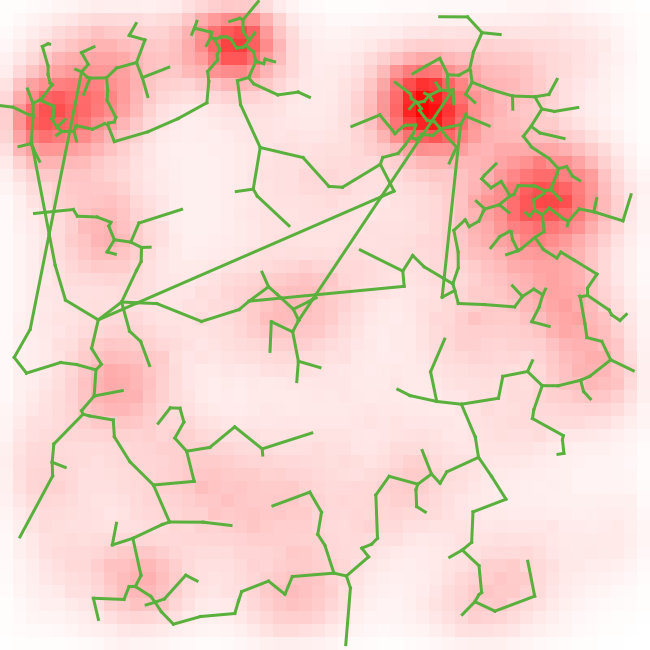
\includegraphics[width=\textwidth]{Figures/Cover/cover} \\ \vspace{3cm} % Picture

\mySubtitle \\ \medskip % Thesis subtitle
%Under the supervision of \myProf and \myOtherProf \\ \medskip
Sous la direction de \myProf et \myOtherProf \\ \medskip
%\myDegree \\
\myDepartment \\  \medskip
\myFaculty \\  \bigskip
%\myUni \\ \bigskip

\myTime\ -- \myVersion % Time and version

\vfill

\end{center}
\end{addmargin}

\end{titlepage} % Main title page

% Back of the title page

\thispagestyle{empty}

\hfill

\vfill

\noindent\myName: \textit{\myTitle,} \mySubtitle, %\myDegree, 
\textcopyright\ \myTime

% You may wish to do something with the back of the title page, such as including your supervisors, location or time frame of the work. Below is an example of doing so although you may want to tweak it to your liking.

%\bigskip

%\noindent\spacedlowsmallcaps{Supervisors}: \\
%\myProf \\
%\myOtherProf \\ 
%\mySupervisor

%\medskip \\

%\noindent\spacedlowsmallcaps{Location}: \\
%\myLocation

%\medskip \\

%\noindent\spacedlowsmallcaps{Time Frame}: \\
%\myTime
 % Back of the title page

\cleardoublepage% Dedication

\thispagestyle{empty}
\refstepcounter{dummy}

\pdfbookmark[1]{Dedication}{Dedication} % Bookmark name visible in a PDF viewer

\vspace*{3cm}



\bpar{
Our relation to our environment and people change at time scales we generally expect larger. Social relations are neither stationary nor in any kind of equilibrium at any time. They are chaos and complexity, as one's mind. As a witness, we include this preliminary dedication, for comparison purposes with the final version.
}{

}


%\begin{center}
%\emph{Ohana} means family. \\
%Family means nobody gets left behind, or forgotten. \\ \medskip
%--- Lilo \& Stitch    
%\end{center}
%
%\medskip
%
%\begin{center}
%Dedicated to the loving memory of Rudolf Miede. \\ \smallskip
%1939\,--\,2005
%\end{center} % Dedication page

\cleardoublepage% Abstract

%\renewcommand{\abstractname}{Abstract} % Uncomment to change the name of the abstract

\pdfbookmark[1]{Abstract}{Abstract} % Bookmark name visible in a PDF viewer

\begingroup
\let\clearpage\relax
\let\cleardoublepage\relax
\let\cleardoublepage\relax

\chapter*{Abstract}
%Short summary of the contents\dots a great guide by 
%Kent Beck how to write good abstracts can be found here:  
%\begin{center}
%\url{https://plg.uwaterloo.ca/~migod/research/beckOOPSLA.html}
%\end{center}


Territorial systems exhibit complexity at any levels and for most of their aspects. Related disciplines generally embrace complex systems science approaches to tackle their understanding and the associated dramatic social and environmental issues. Choosing a specific angle of lecture of territories, it appears, following territorial theories of networks, that real networks play a crucial role in system dynamics, and in particular transportation networks. Taking furthermore a modeling paradigm, we ask to what extent a modeling approach to territorial systems as networked human territories can help disentangling complexly involved processes. We propose to build an associated theory, relying on a vision of human territories as networked, combined with the evolutive urban theory and insights from morphogenesis and co-evolution, that we call a \emph{theory of co-evolutive networked territorial systems}. It is then embedded into a more general epistemological framework insisting on the notions of emergence and modularity. Quantitative epistemological analysis confirm the manual literature review and guide research towards co-evolutive models of networks and territories. We search for stylized facts in empirical datasets to also guide model construction. Methodological developments allow to expect information on dynamical processes from static correlations between urban morphology and network shape. The first modeling experiments include a calibrated spatial model of urban growth, giving an insight into theoretical assumption of network necessity. This model is then weakly coupled with a network generation heuristic to explore the space of feasible correlations. It paves the road for both comparison with real correlations and a strongly coupled calibrated model. We also explore novel paradigms such as the role of governance processes in network growth, through a game-theoretic agent-based model. These preliminary results provide the roadmap towards a family of comprehensive operational models of co-evolution between networks and territories that aim to disentangle their circular causalities.






\endgroup			

\vfill % Abstract page



\cleardoublepage
% Abstract

%\renewcommand{\abstractname}{Abstract} % Uncomment to change the name of the abstract

\pdfbookmark[1]{Reading Notes}{Reading Notes} % Bookmark name visible in a PDF viewer

\begingroup
\let\clearpage\relax
\let\cleardoublepage\relax
\let\cleardoublepage\relax

\chapter*{Reading Notes}

\textit{This provisory Memoire must be read as a work in progress, as it details progresses after one year of Doctorate. Many parts are given at the state of project, and not omitted as playing a role in the current research questioning. Its purpose is to set up a plan and examine the achieved work and corresponding directions, but also to share research ideas at this important step of one year.}




\endgroup			

\vfill



 % Uncomment and create a Foreword.tex to include a foreword



\cleardoublepage% Publications - a page listing research articles written using content in the thesis

\pdfbookmark[1]{Publications}{Publications} % Bookmark name visible in a PDF viewer

\chapter*{Publications} % Publications page text

%Some ideas and figures have appeared previously in the following publications:\\

%\noindent Put your publications from the thesis here. The packages \texttt{multibib} or \texttt{bibtopic} etc. can be used to handle multiple different bibliographies in your document.

%\begin{refsection}[ownpubs]
%    \small
%    \nocite{*} % is local to to the enclosing refsection
%    \printbibliography[heading=none]
%\end{refsection}

%\emph{Attention}: This requires a separate run of \texttt{bibtex} for your \texttt{refsection}, \eg, \texttt{ClassicThesis1-blx} for this file. You might also use \texttt{biber} as the backend for \texttt{biblatex}. See also \url{http://tex.stackexchange.com/questions/128196/problem-with-refsection}.

\bpar{
The following works have an highly overlapping content with this thesis:
}{
Les publications et communications suivantes contiennent la majorité du contenu de cette thèse. Les sources sont précisément mentionnées en introduction de chaque chapitre. Les traductions sont assurées par l'auteur le cas échéant.
}

% NOTE : on self-plagiarism, be careful to precise when extract from a published paper : 
%  - http://academia.stackexchange.com/questions/12342/self-plagiarism-in-phd-thesis
%  - http://academia.stackexchange.com/questions/2029/can-i-use-the-work-in-my-journal-conference-publications-as-chapters-in-my-disse
%  - http://academia.stackexchange.com/questions/149/what-is-a-sandwich-thesis


\section*{Publications}{Publications}


\noindent Raimbault, J. (2017). Identification of Causalities in Spatio-temporal Data, forthcoming in \textit{Sageo 2017 Proceedings.} arXiv:1709.08684

\bigskip

\noindent Raimbault, J. (2017). An Applied Knowledge Framework to Study Complex Systems, forthcoming in \textit{CSD\&M 2017 Proceedings.} arXiv:1706.09244


\bigskip

\noindent Raimbault, J. \& Bergeaud, A. (2017). The Cost of Transportation: Spatial Analysis of Fuel Prices in the US, forthcoming in \textit{Transportation Research Procedia, EWGT 2017.} arxiv:1706.07467


%\bigskip

%\noindent Antelope, C., Hubatsch, L., Raimbault, J., and Serna, J. M. (2016). An interdisciplinary approach to morphogenesis. Forthcoming in Proceedings of Santa Fe Institute CSSS 2016.

\bigskip

\noindent Bergeaud, A., Potiron, Y., \& Raimbault, J. (2017). Classifying patents based on their semantic content. \textit{PloS one, 12}(4), e0176310.

\bigskip

\noindent Raimbault, J. (2017). A Discrepancy-Based Framework to Compare Robustness Between Multi-attribute Evaluations. In \textit{Complex Systems Design \& Management} (pp. 141-154). Springer International Publishing. \cite{raimbault2017discrepancy}

\bigskip

\noindent Raimbault, J. (2017). Investigating the empirical existence of static user equilibrium. \textit{Transportation Research Procedia}, 22, 450-458. \cite{raimbault2017investigating}


\bigskip


\noindent Raimbault, J. (2016). Generation of Correlated Synthetic Data, forthcoming in \textit{Actes des Journ{\'e}es de Rochebrune 2016.}


\bigskip

\noindent Raimbault, J. (2015). Models Coupling Urban Growth and Transportation Network Growth: An Algorithmic Systematic Review Approach, forthcoming in \textit{ECTQG 2015 proceedings.} arxiv:1605.08888


\section*{Communications}{Communications}




\noindent Complexity, Complexities and Complex Knowledge, \textit{Geodivercity International Workshop, Paris, October 2017.}


\bigskip


\noindent Modeling the Co-evolution of Urban Form and Transportation Networks, \textit{Conference on Complex Systems 2017, Cancun, Sept. 2017.}

\bigskip

\noindent Raimbault J. \& Baffi S. (2017). Structural Segregation: Assessing the impact of South African Apartheid on Underlying Dynamics of Interactions between Networks and Territories, \textit{ECTQG 2017, York, Sept. 2017}


\bigskip


\noindent Invisible Bridges ? Scientific landscapes around similar objects studied from Economics and Geography perspectives, \textit{ECTQG 2017, York, Sept. 2017}


\bigskip


\noindent Cottineau C., Raimbault J., Le Texier M., Le N{\'e}chet F. \& Reuillon R. (2017). Initial spatial conditions in simulation models: the missing leg of sensitivity analyses?, \textit{Geocomputation 2017, Leeds, Sept. 2017}

\bigskip


\noindent A macro-scale model of co-evolution for cities and transportation networks, \textit{Medium International Conference, Guangzhou, June 2017}


\bigskip

\noindent Losavio C. \& Raimbault J. (2017). Agent-based Modeling of Migrant Workers Residential Dynamics within a Mega-city Region: the Case of Pearl River Delta, China, \textit{Urban China Development International Conference, London, May 2017}


\bigskip

\noindent Co-construire Modèles, Etudes Empiriques et Théories en Géographie Théorique et Quantitative: le cas des Interactions entre Réseaux et Territoires. In \textit{Treizièmes Rencontres de ThéoQuant, Besançon, Mai 2017}


\bigskip

\noindent Un Cadre de Connaissances pour une Géographie Intégrée. In \textit{Journée des jeunes chercheurs de l'Institut de Géographie de Paris, Paris, April 2017}


\bigskip


\noindent Towards a Theory of Co-evolutive Networked Territorial Systems: Insights from Transportation Governance Modeling in Pearl River Delta, China, \textit{MEDIUM Seminar : Sustainable Development in Zhuhai, Guangzhou, Dec 2016.}


\bigskip


\noindent Models of growth for system of cities : Back to the simple, \textit{Conference on Complex Systems 2016, Amsterdam, Sep 2016.}



%Raimbault J., Bergeaud A. and Potiron Y. (2016). Investigating Patterns of Technological Innovation. \textit{Conference on Complex Systems 2016, Amsterdam, Sep 2016.}


\bigskip

\noindent For a Cautious Use of Big Data and Computation. \textit{Royal Geographical Society - Annual Conference 2016 - Session : Geocomputation, the Next 20 Years (1), London, Aug 2016.}


\bigskip

\noindent Indirect Bibliometrics by Complex Network Analysis. \textit{20e Anniversaire de Cybergeo, Paris, May 2016.}


\bigskip

\noindent Raimbault, J. \& Serra, H. (2016). Game-based Tools as Media to Transmit Freshwater Ecology Concepts, \textit{poster corner at SETAC 2016 (Nantes, May 2016).}


\bigskip

\noindent Le Néchet, F. \& Raimbault, J. (2015). Modeling the emergence of metropolitan transport authority in a polycentric urban region, \textit{ECTQG 2015, Bari, Sep 2015).}


\bigskip

\noindent Hybrid Modeling of a Bike-Sharing Transportation System, \textit{poster presented at ICCSS 2015, Helsinki, June 2015.}

\bigskip

\noindent Raimbault, J. \& Gonzales, J. (2015). Application de la Morphog{\'e}n{\`e}se de R{\'e}seaux Biologiques {\`a} la Conception Optimale d'Infrastructures de Transport, \textit{poster presented at Rencontres du Labex Dynamite, Paris, May 2015.}


 % Publications from the thesis page

%\cleardoublepage% Acknowledgements

\pdfbookmark[1]{Acknowledgements}{Acknowledgements} % Bookmark name visible in a PDF viewer

\begin{flushright}{\slshape    
We have seen that computer programming is an art, \\ 
because it applies accumulated knowledge to the world, \\ 
because it requires skill and ingenuity, and especially \\
because it produces objects of beauty.} \\ \medskip
--- \defcitealias{knuth:1974}{Donald E. Knuth}\citetalias{knuth:1974} \citep{knuth:1974}
\end{flushright}

\bigskip

%----------------------------------------------------------------------------------------

\begingroup

\let\clearpage\relax
\let\cleardoublepage\relax
\let\cleardoublepage\relax

\chapter*{Acknowledgements}

\noindent Put your acknowledgements here.\\

\noindent Many thanks to everybody who already sent me a postcard!\\

\noindent Regarding the typography and other help, many thanks go to Marco Kuhlmann, Philipp Lehman, Lothar Schlesier, Jim Young, Lorenzo Pantieri and Enrico Gregorio\footnote{Members of GuIT (Gruppo Italiano Utilizzatori di \TeX\ e \LaTeX )}, J\"org Sommer, Joachim K\"ostler, Daniel Gottschlag, Denis Aydin, Paride Legovini, Steffen Prochnow, Nicolas Repp, Hinrich Harms, Roland Winkler, and the whole \LaTeX-community for support, ideas and some great software.

\bigskip

\noindent\emph{Regarding \mLyX}: The \mLyX\ port was initially done by
\emph{Nicholas Mariette} in March 2009 and continued by
\emph{Ivo Pletikosi\'c} in 2011. Thank you very much for your work and the contributions to the original style.

\endgroup % Acknowledgements page

\pagestyle{scrheadings} % Show chapter titles as headings

\cleardoublepage% Table of Contents - List of Tables/Figures/Listings and Acronyms

\refstepcounter{dummy}

\pdfbookmark[1]{\contentsname}{tableofcontents} % Bookmark name visible in a PDF viewer

\setcounter{tocdepth}{1} % Depth of sections to include in the table of contents - currently up to subsections

\setcounter{secnumdepth}{2} % Depth of sections to number in the text itself - currently up to subsubsections

\manualmark
\markboth{\spacedlowsmallcaps{\contentsname}}{\spacedlowsmallcaps{\contentsname}}
\tableofcontents 
\automark[section]{chapter}
\renewcommand{\chaptermark}[1]{\markboth{\spacedlowsmallcaps{#1}}{\spacedlowsmallcaps{#1}}}
\renewcommand{\sectionmark}[1]{\markright{\thesection\enspace\spacedlowsmallcaps{#1}}}

\clearpage

\begingroup 
\let\clearpage\relax
\let\cleardoublepage\relax
\let\cleardoublepage\relax

%----------------------------------------------------------------------------------------
%	List of Figures
%----------------------------------------------------------------------------------------

\refstepcounter{dummy}
%\addcontentsline{toc}{chapter}{\listfigurename} % Uncomment if you would like the list of figures to appear in the table of contents
\pdfbookmark[1]{\listfigurename}{lof} % Bookmark name visible in a PDF viewer

\listoffigures

\vspace{8ex}
%\newpage

%----------------------------------------------------------------------------------------
%	List of Tables
%----------------------------------------------------------------------------------------

\refstepcounter{dummy}
%\addcontentsline{toc}{chapter}{\listtablename} % Uncomment if you would like the list of tables to appear in the table of contents
\pdfbookmark[1]{\listtablename}{lot} % Bookmark name visible in a PDF viewer

%\chapter*{List of Tables}

\phantomsection

\listoftables
        
\vspace{8ex}
\newpage
    
%----------------------------------------------------------------------------------------
%	List of Listings
%---------------------------------------------------------------------------------------- 

%\refstepcounter{dummy}
%\addcontentsline{toc}{chapter}{\lstlistlistingname} % Uncomment if you would like the list of listings to appear in the table of contents
%\pdfbookmark[1]{\lstlistlistingname}{lol} % Bookmark name visible in a PDF viewer

%\lstlistoflistings 

%\vspace{8ex}
%\newpage
       
%----------------------------------------------------------------------------------------
%	Acronyms
%----------------------------------------------------------------------------------------

%\refstepcounter{dummy}
%\addcontentsline{toc}{chapter}{Acronyms} % Uncomment if you would like the acronyms to appear in the table of contents
%\pdfbookmark[1]{Acronyms}{acronyms} % Bookmark name visible in a PDF viewer

%\markboth{\spacedlowsmallcaps{Acronyms}}{\spacedlowsmallcaps{Acronyms}}

%\chapter*{Acronyms}

%\begin{acronym}[ABM]
%\acro{ABM}{Agent-based Modeling}
%\acro{API}{Application Programming Interface}
%\acro{UML}{Unified Modeling Language}
%\end{acronym}  
             
             

%\begin{acronym}[SOC]
%\acro{ABM}{Self-organized Criticality}
%\end{acronym} 
             
             
             
                   
\endgroup % Contents, list of figures/tables/listings and acronyms

\cleardoublepage

\pagenumbering{arabic} % Arabic page numbering for thesis content (1, 2, 3, etc)
%\setcounter{page}{90} % Uncomment to manually start the page counter at an arbitrary value (for example if you wish to count the pre-content pages in the page count)

\cleardoublepage % Avoids problems with pdfbookmark

%----------------------------------------------------------------------------------------
%	THESIS CONTENT - CHAPTERS
%----------------------------------------------------------------------------------------



%\ctparttext{}





%%%%%%%%%%%%%%%%
%%  Introduction
%%%%%%%%%%%%%%%%


%% Contents
%
%    - General considerations on Complex Systems, positioning etc (thesis in cs science etc)
%    - Thematic introduction, geographical introduction of the subject.
%
%   - precisions on v1 memoire : foreword ?
%
%    - reading precisions : organisation, interdependances etc 
%
%   - reflexive aspect : here ?  


\chapter*{Introduction}

% to have header for non-numbered introduction
\markboth{Introduction}{Introduction}

%\headercit{We need to find Banos' tenth modeling law}{Ren{\'e} Doursat}{}
\headercit{It's when you shuffle the anthill that you get a touch of all its complexity.}{Arnaud Banos}{}

% citation self-consistent ? -> seems ok

\bigskip


``In consequence of a technical issue, traffic is interrupted on the line B of RER, for an unknown duration. More information will be given as soon as available''. There is a high probability that someone having lived or spent some time in the metropolitan region of Paris has already heard this frightening announce and endured the difficult consequences the rest of his day. But he might not be aware of the ramifications of causal cascades induced by this not-so-rare event. Territorial Systems, whatever the layers considered in their definitions, will always be extremely complex and interrelations at numerous temporal and spatial scales participate in the emergent behaviors observed at any levels of the system. Martin is a student who daily commutes from Paris to Palaiseau and will miss today a crucial exam, what will have a profound impact on his professional life : implications at a long time scale, small spatial scale and agent granularity. Yuangsi is connecting Orly and Roissy Airports, in his trip from London to Beijing, will miss his plane and his sister's wedding : large spatial scale, short time scale, agent granularity. A collective petition emerges from users, leading to new social organizational patterns and reaction from transportation authority that results in efforts to increase levels of service : mesoscopic temporal and spatial scale, swarm of agents granularity. Looking for causes of the event will also lead to intricate processes at various scales, none of which seems to be a better explication than others : historical railway network in Parisian region shaped further extensions and RER B followed the former \textit{Ligne de Sceaux}, \noun{Delouvrier}'s schema for regional development, and its subsequent partial execution, are elements of explanation of structural weaknesses of Parisian public transportation network~\cite{gleyze2005vulnerabilite} ; commuting patterns consequent to territorial organisation induce an overload of particular lines and thus a necessary increase in exploitation incidents. The list could be developed much longer and each approach related to an already mature scientific body of knowledge in different disciplines such as geography, urban economics, transportation. This amusing anecdote is enough to give a touch of the complexity of territorial systems. Our aim here is to dive into this complexity, and in particular to give an original insight into the study of relations between networks and territories. The choice of this reading position will be largely discussed in a further thematic part. Let for now concentrate on the originality of the point of view that we will take.



%-------------------------------------------------

\section*{Scientific Context : Complexity Has Come of Age}


To better introduce our subject, it is necessary to make the reader aware of the particular scientific context we are working in. It is necessary both to understand the general epistemology underlying research questions, and to be aware of the variety of methods and tools used. Contemporaneous science is progressively taking the shift of complexity in many fields. That also implies an epistemological revolution to abandon strict reductionism that failed in most of its synthesis attempts~\cite{anderson1972more}. Arthur recently recalled~\cite{arthur2015complexity} that a mutation of methods and paradigms was also at stake by the increasing role of computational approaches replacing purely analytical techniques generally self-limited in their modeling and resolution scope. Capturing \emph{emergent properties} in models of complex systems is one of the ways to understand the essence of these new approaches.

These considerations are well known in Social Science (both quantitative and qualitative), in which the complexity of studied agents and systems is the justification of their existence : if humans were particles a whole branch of fields may have never emerged as thermodynamics would have solved most of social issues. \footnote{even if it would probably not have been the case as classical physics also failed in their attempts to include irreversibility and evolutions of Complex Adaptive Systems as Prigogine points out in \cite{prigogine1997end}} 
They are however less known nor accepted in more ``hard'' sciences such as physics : Laughlin develops in~\cite{laughlin2006different} a view of the discipline at least as at a ``frontier of knowledge'' then other fields appearing as less mature. Most of knowledge is of classical nature although a majority of structures and systems would be \emph{self-organized}, what means that the single microscopic laws are not enough to determine macroscopic properties unless system evolution is simulated (more precisely this property can be taken as a definition of emergence on which we will come back further, and self-organization is intrinsically emergent). It corresponds to the first nightmare of Laplace's Deamon developed in~\cite{deffuant2015visions}.


As an informal mix of epistemological positions, methods, and fields of applications, \emph{Complexity Science} relies on typical paradigms such as the centrality of emergence and self-organization in most of phenomena of the real world, which make it lie on a frontier of knowledge closer of us than we can think (Laughlin, op.cit. ). Such concepts are indeed not new, as they were already enlighten by Anderson~\cite{anderson1972more}. Even cybernetics can be related to complexity by seing it as a bridge between technology and cognitive science~\cite{wiener1948cybernetics}. Later, synergetics~\cite{haken1980synergetics} paved the way for a theoretical approach of collective phenomena in physics. Reasons for the recent growth of works claiming a CS approach may be various. The explosion of computing power is surely one because of the central role of numerical simulations~\cite{varenne2010simulations}. They could also be the related epistemological progresses : apparition of the notion of perspectivism~\cite{giere2010scientific}, finer reflexions around the notion of model~\cite{varenne2013modeliser}\footnote{In that frame scientific and epistemological progress can not be dissociated and can be seen as coevolving}. The theoretical and empirical potentialities of such approaches play surely a role in their success\footnote{
Although the adoption of new scientific practices may be strongly biased by imitation and lack of originality~\cite{dirk1999measure}, or more ambivalent, by marketing strategies as the fight for funds is becoming a huge obstacle for research~\cite{bollen2014funding}.}, as confirmed in various domains of application (see~\cite{newman2011complex} for a general survey), as for example Network Science~\cite{barabasi2002linked} ; Neuroscience~\cite{koch1999complexity}; Social Sciences ; Geography~\cite{manson2001simplifying}\cite{pumain1997pour} ; Finance with the rising importance of econophysics~\cite{stanley1999econophysics} ; Ecology~\cite{grimm2005pattern}. The Complex Systems Roadmap~\cite{2009arXiv0907.2221B} proposed a double lecture of studies on Complex Systems : an horizontal approach connecting fields of study with transversal questions on theoretical foundations of complexity and empirical common stylized facts, and a vertical conceptions of disciplines, with the aim to construct integrated disciplines and corresponding multi-scale heterogeneous models. Interdisciplinarity is thus central in our scientific background.



\section*{Interdisciplinarity}

%\textit{Note : that term does not exist in english but is a rough translation from french \emph{interdisciplinarit{\'e}}, that we believe to better express }
%
%
%WHY and HOW is interdisciplinarity essential ?
%
% Q : quote Morin ?
%


We must further insist on the role of interdisciplinarity in the positions taken here. This is not a thesis in Geography nor in Complex Adaptive Systems Modeling, but in \emph{Complex Systems Science} that we claim as a proper discipline following \noun{Paul Bourgine}. It will naturally be seen with defiance by scholars of various concerned disciplines, as recent examples of misunderstandings and conflicts have illustrated~\cite{dupuy2015sciences}. The positioning of \noun{Batty} proposing \textit{A new Science of Cities}~\cite{batty2013new} (that he subtly presents as \textit{The} new science of cities) is directed towards an integration of disciplines and methods into a science defined by its object of study, cities. Its theoretical and epistemological weaknesses (no theoretical constructions of studied geographical objects on the one hand, approximative contextualization of complexity) combined with an overall impression of \emph{pot-pourri} of forgotten works (space syntax, land-use models), unfortunately avoid us to use it as we will use geographical theories (e.g. evolutive urban theory) in an appropriated epistemological complexity context. Yet our reading of this work may be the result of a misunderstanding due to different cultural backgrounds.


%\subsection*{Conflicting Complexities and Cultural Differences}

The scientific evolution of complexity that some see as a revolution~\cite{colander2003complexity}, or even as \emph{a new kind of science}~\cite{wolfram2002new}, could indeed face intrinsic difficulties due to behaviors and a-priori of researchers as human beings. More precisely, the need of interdisciplinarity that makes the strength of Complexity Science may be one of its greatest weaknesses, since the highly partitioned structure of science organization has sometimes negative impacts on works involving different disciplines. We do not tackle the issue of over-publication, competition, indexes, which is more linked to a question of open science and its ethics, also of high importance but of an other nature. That barrier we are dealing with and we might struggle to triumph of, is the impact of certains \emph{cultural disciplinary differences} and out-coming conflicts on views and approaches. 
The drama of scientific misunderstandings is that they can indeed annihilate progresses by interpreting as a falsification some work that answers to a totally different question. The example of a recent work on top-income inequalities given in~\cite{aghion2015innovation}, which conclusions are presented as opposed from the one obtained by Piketty~\cite{piketty2013capital}, follows such a scheme. Whereas Piketty focused on constructing long-time clean databases for income data and showed empirically a recent acceleration of income inequalities, his simple model aiming to link this stylized fact with the accumulation of capital has been criticized as oversimplified. On the other hand, Bergeaud \textit{et al.} prove by a model of innovation economics that \emph{under certain assumptions} income gaps may be beneficial to innovation and consequently a general utility. Thus diverging conclusions about the role of personal capitals in the economy. But diverging \emph{views} or \emph{interpretations} does not mean a scientific incompatibility, and one could imagine try to gather both approaches in an unified framework and model, yielding possibly similar or different interpretations. This integrated approach has chances to contain more information (depending on how coupling is done) and to be a further advance in Science. We shall now briefly develop other examples to give an overview how conflicts between disciplines can be damaging.


\paragraph{Physics reinvents geography.}

As already mentioned, \noun{Dupuy} and \noun{Benguigui} points out in \cite{dupuy2015sciences} the fact that urban sciences have recently known open conflicts between old tenants of the disciplines and new arrivants, especially physicists. The availability of large datasets of new type of data (social networks, ICT data) have drawn their attention towards the study of objects traditionally studied by human science, as analytical and computational methods of statistical physics became applicable. Although these studies are generally presented as the construction of a scientific approach to cities, implying that existing knowledge was not scientific because of their more qualitative aspect, they have not unveil specifically novel knowledge on urban systems : to give some examples, \cite{barthelemy2013self} concludes that Paris has followed a transition during Haussman period and that the evolution of a city is the combination of local transformations and global planning operations, what are facts known for a long time in urban history and urban geography. \cite{chen2009urban} rediscovers that the gravity model can be improved by adding lags in interactions and theoretically derives the expression of the force of interaction between cities, without any thematic theoretical background. Examples could be multiplied, confirming the current discomfort in communication between physicists and urban geographers. Significant benefices could results from a wise integration of disciplines~\cite{o2015physicists} but the road seems still long.

\paragraph{Economic Geography or Geographical Economics ?}

Similar conflict occurred in economics : as \cite{marchionni2004geographical} describes, the discipline of economic geography, traditionally close from geography, heavily criticized a new stream of thought named \emph{geographical economics}, which purposes is spatialization of mainstream economic techniques. Both do not have the same purposes and aims, and the conflict appears as a total misunderstanding for an external observer.


\paragraph{Agent-based Modeling in Economy}

Disciplinary conflicts may also manifest themselves as the reject of novel methods by mainstream currents. Following \cite{farmer2009economy}, the operational failure of most classic economic approaches could be compensated by a broader use of agent-based modeling and simulation practices. The lack of analytical framework that is natural in the study of complex adaptive systems seems to be rebutting for most of economists.


\paragraph{Finance}

In Quantitative Finance coexist various stream of research with a very few interactions. Let consider two examples. On the one hand, Statistics are highly advanced in theoretical mathematics, using stochastic calculus and probabilities to obtain very refined estimators of parameters for a given model (see e.g. \cite{barndorff2011multivariate}). On the other hand, Econophysics aims to study empirical stylized facts and infer empirical laws to explain complexity-related phenomena in financial systems~\cite{stanley1999econophysics}, such as e.g. cascades leading to market crashes, fractal properties of asset signals, complex structure of correlation networks. Both have their advantages in a particular context and each would benefit from increased interactions between the fields.


\bigskip

These diverse examples illustrate how interdisciplinarity is both crucial and difficult to achieve. We will try to follow that narrow path in our work, borrowing ideas, theories and methods from various disciplines, aiming for the construction of an integrated knowledge. Indeed, coupling heterogeneous approaches at different levels and scales will be a cornerstone of our thesis, skeleton of the underlying philosophy and building brick of the theory we will propose.







%-------------------------------------------------

\section*{Complexity in Geography}


Coming back to our introducing anecdote, we will focus on our thematic object of study that are territorial systems. More generally, we propose an overview of the role of complexity in geography. Geographers are familiar with complexity for a long time, as the study of spatial interactions is one of its purposes. The variety of fields in geography (geomorphology, physical geography, environmental geography, human geography, health geography to give a few) has certainly been important in the subtlety of the geographical thinking, that considers heterogeneous and multi-scalar processes.

\noun{Pumain} recalls in~\cite{pumain2003approche} a subjective history of the emergence of complexity paradigms in geography. Cybernetics yielded system theories as the one developed by Forrester. Later the shift to self-organized criticality and self-organisation concepts in physics conducted to corresponding developments in geography, as \cite{sanders1992systeme} witnesses the application of the concepts of synergetics for the dynamics of an urban system. Finally, Complex Systems paradigms as we currently know them appeared from various points of view. For example, the fractal nature of urban shape was introduced in~\cite{batty1994fractal} and had numerous application including more recent developments~\cite{keersmaecker2003using}. \noun{Batty} also introduced cellular automata in urban modeling and proposed a joint synthesis with agent-based modeling and fractals in~\cite{batty2007cities}. An other incursion of complexity in geography was for the case of urban systems through the evolutive urban theory of \noun{Pumain}. In close relation with modeling from the beginning (the first Simpop model described in~\cite{sanders1997simpop} enters the theoretical framework of \cite{pumain1997pour}), this theory aims to understand system of cities as systems of co-evolving adaptive agents, interacting in many ways, with particular features emphasized such as the diffusion of innovation. The series of Simpop models~\cite{pumain2012multi} focused in testing various assumptions of the theory. For example, different underlying mechanisms were revealed for european city systems and city system of the united states~\cite{bretagnolle2010comparer}. At other time scales and in other contexts, the SimpopLocal model~\cite{schmitt2014modelisation} aimed to investigate the conditions for the emergence of hierarchical urban systems from disparate settlements. A minimal model (in the sense of sufficient and necessary parameter) has been isolated thanks to the use of intensive computation with the model exploration software OpenMole~\cite{schmitt2014half}, what was a result analytically not derivable for this kind of complex model. The technical progresses of OpenMole~\cite{reuillon2013openmole} were done simultaneously with theoretical and empirical advancements. Epistemological advances were also essential to this framework, as \noun{Rey} develops in~\cite{rey2015plateforme}, and novel concepts such as incremental modeling~\cite{cottineau2015incremental} were found, with powerful concrete applications : \cite{cottineau2014evolution} implemented it on the soviet city system and isolated dominating socio-economic processes, by systematic testing of thematic assumptions and implementation functions. Directions for the development of such Modeling and Simulation practices in quantitative geography were recently introduced by \noun{Banos} in~\cite{banos2013pour}. He concludes with nine principles\footnote{I remember \noun{Ren{\'e} Doursat} insisting on the search of the last commandement of Banos}, from which we can cite the importance of intensive exploration of computational models and the importance of heterogeneous model coupling, that are among other principles such as reproducibility at the center of the study of complex geographical systems from the point of view described just before. Positioning in the legacy of this line of research, we will conjointly work in the theoretical, empirical, epistemological and modeling domains.




\section*{Research Question}


Research question and precise objects are deliberately fuzzy for now, as we postulate that the construction of a problematic can not be dissociated from the production of a corresponding theory. Reciprocally, it makes no sense to ask questions out of the blue, on objects that have been only partially or rapidly defined. Our preliminary question to enter the subject, that we can obtain from concrete cases such as our introducing anecdote or from preliminary literature review, is the following :

\bigskip

\textit{Is it possible to produce a definition of territorial systems, and corresponding scales and ontologies, that would yield a natural, consistent and informational view on processes ?}

\bigskip

Indeed, a necessary characteristic of territorial systems is their spatio-temporal nature, that is contained in spatio-temporal dynamics. The notion of \emph{process} in the sense of \cite{hypergeo} captures furthermore causal relationships in these dynamics, and is thus an interesting approach for an understanding of such systems. \emph{Scale} must be understood here in the operational sense (physical characteristic ) and \emph{ontology} as real-world studied objects\footnote{this use of ontology here naturally biaises our research towards modeling paradigms as it is close from the notion of ontology used in~\cite{livet2010}, but we take the position (largely developed further) to understand any scientific construction as \emph{models}, making the frontier between theory and modeling less relevant than in standard views. Any theory has to make choices on described objects, relations and processes, and therefore contains an ontology in that sense.}. Our question may be roughly viewed as a search for theories and models that would unveil some processes involved in complex systems containing at least human settlements, the last requirement being crucial for a convergent problematic construction rather than ending in non-realistic and non-constructive propositions to understand everything between the brain (that can be seen as one building brick of territorial systems as they emerge from human social constructions) and the ecosphere that includes territorial systems.  




%-------------------------------------------------

\section*{Contents}


This provisory Memoire is organized the following way. A first part with four chapters sets the thematic, theoretical and methodological background. The study of geographical systems implies, because of their complexity, a subtle combination of Theoretical constructions and Empirical Analysis, either in an inductive reasoning or in a didactic constitution of knowledge. The first part aims to approach our subject from the theoretical and methodological point of view, and rather as a \textit{necessary foundation} shall be understood as a body of knowledge \emph{coevolving} with Empirical and Modeling Parts. A linear reading is not necessarily the best way to deeply perceive the implications of theory on empirical and modeling experiments and reciprocally. Some methodological developments are necessary but explicit reference will be done when it will be the case. A first chapter starts from the provisory research question given above and frames from a thematic point of view geographical objects and processes to be studied, resulting in precise research questions. The scene is set up for the construction of our theoretical background in a second chapter, that consists in a geographical theory for territorial systems on the one hand and in an epistemological theory of socio-technical systems modeling that frames our approach at a meta-level. We then develop methodological considerations on diverse questions implied by theory and required for modeling. Finally, a chapter of quantitative epistemology finishes to pave the way for modeling directions, unveiling literature gaps precisely linked to our question. A second part develops results obtained from empirical analysis and modeling experiments, along with on-going and planned projects in these fields. It first present empirical analysis aimed at identifying stylized facts. Toy-models of urban growth are then proposed, followed by an example and propositions for more complex models. The third part constructs our research objective for the remaining part of our project and sets a corresponding roadmap. Appendices contain non-digest important parts of our work such as models implementation architecture and details and specific tools developed for a reproducible research workflow.













  







%----------------------------------------------------------------------------------------

\ctparttext{This part set up foundations, constructing our research precise subject and questions from a thematic point of view, completed with a theoretical construction for framing at thematic and epistemological levels. We also provide methodological digressions, and a quantitative epistemological analysis completing the manual state of the art.} % Text on the Part 1 page describing  the content in Part 1

% Part I : methodology / theory / meta-theory
%\part{Thematic, Theoretical and Methodological Foundations} % First part of the thesis
\part{Foundations : setting up the ground and roots}

% -- Remark : the architectural metaphor is nice to introduce diverse parts --


%%%%%%%%%%%%%%%%%%%%%%%%%%%%%
% Chapter : Quantitative Epistemology


% Chapter 




%\chapter{Interactions between Networks and Territories}{Interactions entre Réseaux et Territoires} % Chapter title
\chapter{Interactions entre Réseaux et Territoires}


\label{ch:thematic} % For referencing the chapter elsewhere, use \autoref{ch:name} 




%----------------------------------------------------------------------------------------

%\headercit{If you are embarrassed by the precedence of the chicken by the egg or of the egg by the chicken, it is because you are assuming that animals have always be the way they are}{Denis Diderot}{\cite{diderot1965entretien}}

%\headercit{Si la question de la priorit{\'e} de l'\oe{}uf sur la poule ou de la poule sur l'\oe{}uf vous embarrasse, c'est que vous supposez que les animaux ont {\'e}t{\'e} originairement ce qu'ils sont {\`a} pr{\'e}sent.
%}{Denis Diderot}{\cite{diderot1965entretien}}


\bigskip


\bpar{
This analogy is ideal to evoke the questions of causality and processes in territorial systems. When trying to tackle naively our preliminary question, some observers have qualified the identification of causalities in complex systems as ``chicken and egg'' problems : if one effect appears to cause another and reciprocally, how can one disentangle effective processes ? This vision is often present in reductionist approaches that do not postulate an intrinsic complexity in studied systems. The idea that Diderot suggests is the notion of \emph{co-evolution} that is a central phenomenon in evolutive dynamics of Complex Adaptive Systems as \noun{Holland} develops in~\cite{holland2012signals}. He links the notion of emergence (that is ignored in a reductionist vision), in particular the emergence of structures at an upper scales from the interactions between agents at a given scale, materialized generally by boundaries, that become crucial in the coevolution of agents at any scales : the emergence of one structure will be simultaneous with one other, each exploiting their interrelations and generated environments conditioned by their boundaries. We shall explore these ideas in the case of territorial systems in the following.
}{
Pour mieux visualiser les notions de causalités circulaires dans les systèmes complexes, et pourquoi celles-ci peuvent conduire à des paradoxes en apparence, l'image fournie par \noun{Diderot} dans~\cite{diderot1965entretien} est idéale : ``\textit{Si la question de la priorit{\'e} de l'\oe{}uf sur la poule ou de la poule sur l'\oe{}uf vous embarrasse, c'est que vous supposez que les animaux ont {\'e}t{\'e} originairement ce qu'ils sont {\`a} pr{\'e}sent}''. En voulant traiter naïvement des questions similaires induites par notre problématique introduite précédemment, certains ont qualifié les causalités au sein de systèmes complexes géographiques comme un problème ``de poule et {\oe}uf'' : si un effet semble causer l'autre et réciproquement, est-il possible et même pertinent de vouloir isoler les processus correspondants ? Cette question est bien connue des planificateurs des transports, comme le rappelle la notion des ``effets structurants'' qui fait débat depuis un certain temps au moins dans la communauté scientifique \comment[FL]{non cela va trop vite}. Une vision simplifiée, selon laquelle on peut attribuer des rôles systématiques à une composante particulière, est souvent présente dans les approches réductionnistes qui ne postulent pas une complexité intrinsèque au sein des systèmes étudiés.\comment[FL]{mots pas clairs ; a la place : amener co-evolution} L'idée suggérée par \noun{Diderot} est celle de \emph{co-evolution} qui est un phénomène central dans les dynamiques évolutionnaires des Systèmes Complexes Adaptatifs comme \noun{Holland} élabore dans~\cite{holland2012signals}. Il fait le lien entre l'émergence de structures à une échelle supérieure par les interactions entre agents à une échelle donnée, en général concrétisée par un systèmes de limites\comment[FL]{pas clair}, qui devient cruciale pour la co-évolution des agents à toutes les échelles : l'émergence d'une structure sera simultanée avec une autre, chacune exploitant leur interrelations et environnements générés conditionnés par le système de limites.\comment[FL]{rupture : le fil n'est pas clair} Nous explorerons ces idées pour le cas des systèmes territoriaux par la suite. Ceux-ci illustrent parfaitement ces problématiques, et sont typiques de systèmes dans lesquels cette complexité\comment[FL]{laquelle} est cruciale pour une appréhension raisonnable des mécanismes impliqués dans leurs dynamiques. Un certain nombre d'illustrations concrètes\comment[FL]{de quoi ?} seront d'abord données pour formuler nos questionnements dans des contextes géographiques donnés.\comment[FL]{phrase inutile}
}



\bpar{
This introductive chapter aims to set up the thematic scene, the geographical context in which further developments will root. It is not supposed to be understood as an exhaustive literature review nor the fundamental theoretical basement of our work (the first will be an object of chapter~\ref{ch:quantepistemo} whereas the second will be earlier tackled in chapter~\ref{ch:theory}), but more as narration aimed to introduce typical objects and views and construct naturally research questions.
}{
Ce chapitre introductif est destiné à poser le cadre thématique, les contextes géographiques sur lesquels les développements suivants se baseront.\comment[FL]{plus haut} Il n'est pas supposé être compris comme une revue de littérature exhaustive ni comme les fondations théoriques fondamentales de notre travail, le premier point étant l'objet du chapitre~\ref{ch:modelinginteractions} tandis que le second sera traité systématiquement dans le chapitre~\ref{ch:theory} lorsque le recul nécessaire aura été progressivement construit. Il doit plutôt être lu comme une construction narrative ayant pour but d'introduire nos objets et positions d'étude.\comment[FL]{cela sera dans l'intro generale} La notion de co-évolution est particulièrement pertinente\comment[FL]{oui : a remonter} pour comprendre les interactions entre territoires et réseaux. Dans une première section~\ref{sec:networkterritories}, nous préciserons l'approche prise de l'objet territoire, et dans quelle mesure celui-ci naturellement implique la considération des réseaux de transport pour la compréhension des dynamiques couplées. Ces considérations abstraites seront illustrées par des cas d'étude concrets dans la deuxième section~\ref{sec:casestudies}, choisis très différents pour comprendre les enjeux d'universalité sous-jacents. Enfin, dans la troisième section~\ref{sec:qualitative},des éléments d'observation de terrain effectués en Chine préciseront encore ces exemples aux échelles microscopique et mesoscopique. \comment[FL]{reprendre}
}



\stars


\textit{Ce chapitre est entièrement inédit.}\comment[FL]{ne pas dire cela}[(JR) permet d'avoir une unite avec les autres chapitres.]







%-------------------------------




























%%%%%%%%%%%%%%%%%%%%%%%%%%%%%





%%%%%%%%%%%%%%%%%%%%%%%%%%%%%
% Chapter : Theoretical Framework




%----------------------------------------------------------------------------------------

\newpage

% first section that develops elements of geographical theory : system of cities, territories, etc.
%  city morphogenesis ? -> link to other approaches of morphogenesis (Turing)
%  coevolution : give a precise theoretical meaning

% HERE precise exact definition, framed precisely (reference for the following).

\section{Geographical Theoretical Context}{Pour une Théorie Géographique}



%%%%%%%%%%%
\subsection{Foundations}{Fondations}



%%%%%%%%%%%%%%
\subsubsection{Networked Human Territories}{Territoires Humains en Réseau}


\bpar{
Our first pillar has already been constructed before in the thematic exploration of the research subject. We rely on the notion of \emph{Human Territory} elaborated by \noun{Raffestin} as the basis for a definition of territorial systems. It permits to capture complex human geographical systems in their concrete and abstract characteristics and representation. For example, a metropolitan territorial system can be apprehended simply by the functional extent of daily commuting, or by the perceived or lived space of different populations, the choice depending on the precise question asked. Note that this approach to territory is a position and that other (possibly compatible) entries could be taken~\cite{murphy2012entente}. The concrete of this pillar in reinforced by the territorial theory of networks of \noun{Dupuy}, yielding the notion of networked human territory, as a human territory in which a set of potential transactional networks have been realized, which is in accordance with vision of the territory as networked places~\cite{champollion:halshs-00999026}. We make therein the assumption that real networks are necessary elements of territorial systems.
}{
Notre premier pilier a déjà été construit précédemment lors de l'exploration thématique du projet de recherche. Nous nous basons sur la notion de \emph{Territoire Humain} élaborée par \noun{Raffestin} comme la base de la définition d'un système territorial. Elle permet de capturer les systèmes complexes géographiques humains dans l'ensemble de leur caractéristiques concrètes et abstraites, ainsi que dans leur représentations. Par exemple, un territoire métropolitain peut être appréhendé simplement par l'étendue fonctionnelle des flux pendulaires journaliers, ou par l'espace perçu ou vécu des différentes populations, le choix dépendant de la question précise à laquelle on cherche à répondre. Cette approche au territoire est bien sûr un choix délibéré et que d'autres entrées, possiblement compatible, peuvent bien sûr être prises~\cite{murphy2012entente}. Le ciment de ce pilier est renforcé par la théorie territoriale des réseaux de \noun{Dupuy}, fournissant la notion de territoire humain en réseau, comme un territoire humain dans lequel un ensemble de réseaux transactionnels potentiels ont été réalisés, ce qui s'accorde par ailleurs avec les visions du territoire comme un lieu des réseaux~\cite{champollion:halshs-00999026}. % TODO here beware confusion between place and space : lieu en réseau ≠ lieu des réseaux ≠ espace en réseau ≠ espace des réseaux ???
Nous ferons pour cela l'hypothèse fondamentale que les réseaux réels sont des éléments nécessaires des systèmes territoriaux.
\comment{(Florent) déjà dit}
}

%%%%%%%%%%%%%%%
\subsubsection{Evolutive Urban Theory}{Théorie Evolutive des Villes}

% development of Denise theory
%  -> extension with precision on coevolution ? (read Holland on coevolution) -- beware of biological //


\bpar{
The second pillar of our theoretical construction is the Evolutive Urban Theory of \noun{Pumain}, closely linked to the complexity approach we take. This theory was first introduced in~\cite{pumain1997pour} which argues for a dynamical vision of city systems, in which self-organization is key. Cities are interdependent evolutive spatial entities whose interrelations produces the macroscopic behavior at the scale of city system. The city system is also designed as a network of city what emphasizes its view as a complex system. Each city is itself a complex system in the spirit of~\cite{berry1964cities}, the multi-scale aspect being essential in this theory, since microscopic agents convey system evolution processus through complex feedbacks between scales. The positioning within Complex System Sciences was later confirmed~\cite{pumain2003approche}. It was shown that this theory provide an interpretation for the origin of pervasive scaling laws, resulting from the diffusion of innovation cycles between cities~\cite{pumain2006evolutionary}. The aspect of resilience of system of cities, induced by the adaptive character of these complex systems, implies that cities are drivers and adapters of social change~\cite{pumain2010theorie}. Finally, path dependance yield non-ergodicity within these systems, making ``universal'' interpretations of scaling laws developed by physicists incompatible with evolutive urban theory~\cite{pumain2012urban}. The Evolutive Urban Theory was elaborated conjointly with models of urban systems: for example the Simpop2 model is an agent-based model taking into account economic processes, that simulates growth patterns on long time scales for Europe and the United States~\cite{doi:10.1177/0042098010377366}. % TODO \cite{bretagnolle2006theory} introduction of simpop2 model // remove french versions ?
 The latest accomplishment of the evolutive theory relies in the output of the ERC project GeoDivercity, presented in~\cite{pumain2017urban}, that include both advanced technical (software OpenMole), thematic (knowledge from SimpopLocal and Marius models) and methodological (incremental modeling) progresses. We will interpret territorial systems following that idea of complex adaptive systems.
}{
Le second pilier de notre construction théorique est la théorie évolutive des villes de \noun{Pumain}, en relation étroite avec l'approche complexe que nous prenons de manière générale. Cette théorie a été introduite initialement dans~\cite{pumain1997pour} qui argumente pour une vision dynamique des systèmes de ville, au sein desquels l'auto-organisation est essentielle. Les villes sont des entités spatiales évolutives interdépendantes dont les interrelations font émerger le comportement macroscopique à l'échelle du système de villes. Le système de villes est aussi vu comme un réseau de villes, ce qui renforce sa vision en tant que système complexe. Chaque ville est elle-même un système complexe dans l'esprit de~\cite{berry1964cities}, l'aspect multi-scalaire \comment{(Florent) tu n'as toujours pas concrètement expliqué ce que c'était}
étant essentiel dans cette théorie, puisque les agents microscopiques véhiculent les processus d'évolution du système à travers des rétroactions complexes entre les échelles. Le positionnement de cette théorie au regard des Sciences des Systèmes Complexes a plus tard été confirmé~\cite{pumain2003approche}. Il a été montré que la théorie évolutive fournit une interprétation des lois d'échelle qui sont omniprésentes dans les systèmes urbains, qui découleraient de la diffusion des cycles d'innovation entre les villes~\cite{pumain2006evolutionary}. La notion de résilience d'un système de villes, induit par le caractère adaptatif des ces systèmes complexes, implique que les villes sont les moteurs et les adaptateurs du changement social~\cite{pumain2010theorie}. Enfin, la dépendance au chemin est source de non-ergodicité au sein de ces systèmes, rendant les interprétations ``universelles'' des lois d'échelle développées par les physiciens incompatibles avec la théorie évolutive~\cite{pumain2010theorie}. \comment{(Florent) ergodicité : terme à définir ? ok ?} La Théorie Evolutive des Villes a été élaborée conjointement avec des modèles de systèmes urbains : par exemple le modèle Simpop2 est un modèle basé agent qui prend en compte des processus économiques, et simule sur de longues échelles de temps les motifs de croissance urbaine pour l'Europe et les Etats-unis~\cite{doi:10.1177/0042098010377366}. L'accomplissement le plus récent de la théorie évolutive réside dans la production de l'ERC GeoDivercity, présentée dans~\cite{pumain2017urban}, qui inclut à la fois des progrès techniques avancés (logiciel OpenMole), thématiques (connaissances issues des modèles SimpopLocal et Marius) et méthodologiques (modélisation par incréments). Nous interpréterons les systèmes territoriaux à la lumière de cette idée des villes comme systèmes complexes adaptatifs.
}



%%%%%%%%%%%
\subsubsection{Urban Morphogenesis}{Morphogenèse Urbaine}

% -> make a link between city systems and urban form/cityscape / territorial configurations

% Why morphogenesis is important : linked with modularity and scale -> if a submodule can be explained independantly (ie morphigeneis process is isolated), then we have the characteristic scale. then when size grows and interaction within city system -> can not explain alone (or with externalities ?) -> need a change in scale. ex. influecne of city system for size, activities; posiiton of an airport in a metropoltian region ; emergence of MCR.  ==> Assimptions to be tested with models ?.

% Alexander and Salingaros

% include transportation network, hierarchy and congestion in transport : Remy vs Benjamin (paper ? -> see with René)



\bpar{
The idea of morphogenesis was particularly underlined by \noun{Turing} in~\cite{turing1952chemical} % not exactly, already introduced before
 when trying to isolate simple chemical rules that could lead to the emergence of the embryo and its form. The morphogenesis of a system consists in self-consistent evolution rules that produce the emergence of its successives states, i.e. the precise definition of self-organization, with the additional property that an emergent architecture exists, in the sense of relations between form and function. Progresses towards the understanding of embryo morphogenesis (in particular the isolation of processes producing the differentiation of cells from an unique cell) has been made only recently with the use of Complexity Approaches in integrative biology~\cite{delile2016chapitre}. In the case of urban systems, the idea of urban morphogenesis, i.e. of self-consistent mechanisms that would produce the urban form, is more used in the field of architecture and urban design~\cite{hachi2013master} (as \noun{Alexander} generative grammar ``Pattern Language'' e.g.), in relation with theories of Urban Form~\cite{moudon1997urban}. This idea can be pushed into very small scales such as the building~\cite{whitehand1999urban} but we will use it more at a mesoscopic scale, in terms of land-use changes within an intermediate scale territorial system, in the same ontologies as Urban morphogenesis modeling literature (for example \cite{bonin2012modele} describes a model of urban morphogenesis with qualitative differentiation, whereas \cite{makse1998modeling} give a model of urban growth based on a mono-centric population distribution perturbed with correlated noises). The notion of morphogenesis will be important in our theory in link with modularity and scale. Modularity of a complex system consists in its decomposition into relatively independent sub-modules, and modular decomposition of a system can be seen as a way to disentangle non-intrinsic correlations~\cite{2015arXiv150904386K} (think of a block diagonalisation of a first order dynamical system). In the context of large-scale cyber-physical systems design and control, similar issues naturally raise and specific techniques are needed to scale up simple system control methods~\cite{2017arXiv170105880W}. The isolation of a subsystem yields a corresponding characteristic scale. Isolating possible morphogenesis processes imply a controlled isolation (controlled boundary conditions e.g.) of the considered system, corresponding to a modularity level and thus a scale. When self-consistent processes are not enough to explain the evolution of the system (with reasonable action on boundary conditions), a change of scale is necessary, caused by an underlying phase transition in modularity. The example of metropolitan growth is a good example: complexity of interactions within the metropolitan region will grow with size and diversity of functions leading to a change in scale necessary to understand processes. The emergence of an international airport will strongly influence local development, what corresponds to the significant integration within a larger system. The characteristic scales and processes for which these change occur will be precise questions to be investigated through modeling. It is interesting to remark that a territorial subsystem in which morphogenesis has a sense can be seen as an \emph{autopoietic system} in the extended sense of \noun{Bourgine} in~\cite{bourgine2004autopoiesis}, as a network of auto-reproducing processes\footnote{which are however not cognitive, making this auto-organized systems fortunately not alive in the sense of autopoietic and cognitive systems} regulating their boundary conditions, what emphasizes boundaries on which we will last insist.
}{
La notion de morphogenèse a été particulièrement soulignée par \noun{Turing} dans~\cite{turing1952chemical} lorsqu'il proposait d'isoler des règles chimiques élémentaires qui pourraient mener à l'émergence de l'embryon et à sa forme. La morphogenèse d'un système consiste en des règles d'évolution auto-cohérentes qui produisent l'émergence de ses états successifs, i.e. la définition précise de l'auto-organisation, avec la propriété supplémentaire qu'une architecture émergente existe, au sens de relations entre la forme et la fonction. Les progrès vers la compréhension de la morphogenèse de l'embryon (en particulier l'isolation de processus particuliers induisant la différentiation de cellules à partir d'une unique) sont relativement récents grâce à l'application des approches complexes en biologie intégrative~\cite{delile2016chapitre}. Dans le cas des systèmes urbains, l'idée de morphogenèse urbaine, i.e. de mécanismes auto-cohérents qui produiraient la forme urbaine, est plutôt utilisé dans les champs de l'architecture et de l'urbanisme~\cite{hachi2013master} (comme e.g. la grammaire générative du ``Pattern Language'' d'\noun{Alexander}), en relation avec des théories de la forme urbaine~\cite{moudon1997urban}. Cette idée peut être poussée jusqu'à de très petites échelles comme celle du bâtiment~\cite{whitehand1999urban} mais nous l'utiliserons plus à une échelle mesoscopique, en termes de changements d'usage du sol à une échelle intermédiaire des systèmes territoriaux, avec des ontologies similaires à la littérature de modélisation de la morphogenèse urbaine (par exemple \cite{bonin2012modele} décrit un modèle de morphogenèse urbaine avec différentiation qualitative, tandis que \cite{makse1998modeling} donne un modèle de croissance urbaine basé sur une distribution monocentrique de la population perturbée par des bruits corrélés). La notion de morphogenèse sera importante dans notre théorie en lien avec la modularité et l'échelle. \comment{(Florent) très clair}
La modularité d'un système complexe consiste en sa décomposition en sous-modules relativement indépendants, et la décomposition modulaire d'un système peut être vue comme un moyen de supprimer les correlations non intrinsèques~\cite{2015arXiv150904386K} (pour donner une image, penser à une diagonalisation par blocs d'un système dynamique du premier ordre). Dans le cadre de la conception et du contrôle de systèmes cyber-sociaux à grande échelle, des problèmes similaires surgissent naturellement et des techniques spécifiques sont nécessaires pour le passage à l'échelle des techniques simple de contrôle~\cite{2017arXiv170105880W}. L'isolation d'un sous-système fournit une échelle caractéristique correspondante. Isoler des processus de morphogenèse possibles implique une extraction contrôlée (conditions au bord contrôlées par exemple) du système considéré, ce qui correspond à un niveau de modularité et donc à une échelle. Quand des processus auto-cohérents ne sont pas suffisants pour expliquer l'évolution d'un système (dans des variations raisonnables des conditions initiales), un changement d'échelle est nécessaire, \comment{(Florent)  peut être que des schémas pourraient aider le lecteur}
causé par une transition de phase implicite dans la modularité. L'exemple de la croissance métropolitaine en est une très bonne illustration : la complexité des interactions au sein de la région métropolitaine sera croissante avec sa taille et la diversité des fonctions urbaines, ce qui conduit à un changement de l'échelle nécessaire pour comprendre les processus. L'émergence d'un aéroport international influencera fortement le développement local, \comment{(Florent) pas forcément ici. Ciudad Real}
ce qui correspondant à une intégration significative dans un système plus vaste. Les échelles caractéristiques et la nature des processus pour lesquels ces changements ont lieu peuvent être des questions précisément approchées par l'angle de la modélisation. Il est intéressant \comment{(Florent) oui si on te suit, tout est intéressant..}
de noter qu'un système territorial dans lequel la morphogenèse prend sens peut être vu comme un \emph{système auto-poiétique} % TODO no distinction ?
 au sens étendu de \noun{Bourgine} dans~\cite{bourgine2004autopoiesis}, comme un réseau de processus qui s'auto-reproduisent\footnote{qui ne sont toutefois pas cognitifs, ne rendant heureusement pas ces systèmes auto-organisés vivant au sens de auto-poiétique et cognitif} en régulant leur conditions aux bords, ce qui souligne la notion de frontière sur laquelle nous allons finalement nous attarder.
}


\cite{desmarais1992premisses}
\cite{levy2005formes}


% transition : Bourgine autopoiesis -> importance of boundaries -> link to Holland.

%%%%%%%%%%%
\subsubsection{Co-evolution}{Co-évolution}

% other insight : Holland Signal and Boundaries, ecological niche etc. : contextualize within this framework, clarify definition of co-evolution


\bpar{
Our last pillar is a clarification of the notion of \emph{co-evolution}, on which \noun{Holland} shed light through an approach of complex adaptive systems by a theory of CAS as signal processing agents operating thanks to their boundaries~\cite{holland2012signals}. In this theory, complex adaptive systems form aggregates at diverse hierarchical levels, that correspond to different level of self-organization, and boundaries are vertically and horizontally intricate in a complex way. That approach introduces the notion of \emph{niche} as a relatively independent subsystem in which ressources circulate (the same way as network communities): numerous illustrations are given such as economical niches or ecological niches. Agents within a niche are said to be \emph{co-evolving}. Co-evolution thus means strong interdependences (implying circular causal processes) and a certain independence regarding the exterior of the niche. The notion is naturally flexible as it will depend on ontologies, resolution, thresholds etc. considered to define the system. This concept is easily transmissible to the evolutive urban theory and converges with the notion of co-evolution described by \noun{Pumain}: co-evolving agents in a system of cities consist in a niche with its flows, signals and boundaries and thus co-evolving entities in the sense of \noun{Holland}. This notion will be important for us in the definition of territorial subsystems and their coupling.
}{
Notre dernier pilier consiste en une clarification de la notion de \emph{co-evolution}, sur laquelle \noun{Holland} apporte un éclairage pertinent à travers son approche des systèmes complexes adaptatifs (CAS) par une théorie des CAS comme agents traitant des signaux \comment{(Florent) ? sens ?}
grâce à leur frontières~\cite{holland2012signals}. Dans cette théorie, les systèmes complexes adaptatifs forment des agrégats à différents niveaux hiérarchiques, qui correspondent à différents niveaux d'auto-organisation, et les frontières sont intriquées horizontalement et verticalement de manière complexe. Cette approche introduit la notion de \emph{niche} comme un sous-système relativement indépendant au sein duquel les ressources circulent (de la même façon que des communautés dans un réseau) : de nombreuses illustrations telles les niches écologiques ou économiques peuvent être données. Les agents au sein d'une niche sont dits en \emph{co-évolution}. \comment{(Florent) et y'a t'il des territorial niches ? par ailleurs pourquoi pas tester hypothèse niche mais pourquoi pas autre chose ?}
 La co-évolution implique ainsi de fortes interdépendances (impliquant des processus causaux circulaires) et une certaine indépendance au regard de l'extérieur de la niche. La notion est naturellement flexible puisqu'elle dépendra des ontologies, de la résolution, des seuils, etc. que l'on considère pour définir le système. Ce concept se transmet assez aisément\comment{(Florent) cette facilité ne me semble pas si évidente, notamment l'indépendance avec l'extérieur}
  à la théorie évolutive urbaine et correspond à la notion de co-évolution décrite par \noun{Pumain} : des agents co-évolutifs dans un système de villes consistent en une niche et ses flots, signaux et limites et sont donc des entités co-évolutives au sens de \noun{Holland}. Cette notion sera importante pour nous dans la définition des sous-systèmes territoriaux et de leur couplage.
}

\comment{(Arnaud) Notion de Niche}



%%%%%%%%%%%
%\subsection{Requirements}
% RQ : no requirements for the theory, contained within pillars : requirement is the presence of these pillars ?



%%%%%%%%%%%
\subsection{Synthesis: an theory of co-evolutive networked territorial systems}{Synthèse : une théorie des systèmes territoriaux co-évolutifs en réseau}

% put different elements together and construct the geographical theory
% give here precise definitions

\bpar{
We synthesize our pillars as a short self-consistent geographical theory of territorial systems in which networks play a central role in the co-evolution of components of the system. See the foundation subsection for definitions and references. The formulation is intended to be minimalistic.
}{
Nous synthétisons les différents piliers en une théorie géographique autonome des systèmes territoriaux pour lesquels les réseaux jouent un rôle central pour la co-évolution des composantes du système. Pour les définitions des termes et les références, se référer à la section précédente. La formulation ici est voulue minimaliste.
}


\medskip


\bpar{
\begin{definition}
\textbf{ - Territorial System.} A territorial system is a set of networked human territories, i.e. human territories in and between which real networks exist.
\end{definition}
}{
\begin{definition}
\textbf{ - Système Territorial.} Un système territorial est un ensemble de territoires humains en réseau, c'est à dire des territoires humains au sein desquels et entre lesquels des réseaux réels existent.
\end{definition}
\comment{(Florent) donc territoire $\subset$ système territorial ? discutable, il faut donner de la chair à ces discussions.}
}

\comment{(Florent) a la fin ne garder qu'une définition}


\medskip


\bpar{
At this step complexity and dynamical evolutive characters of territorial systems are implied but not an explicit part of the theory. We will assume to simplify a discrete definition of temporal, spatial and ontological dimensions under modularity and local stationarity assumptions.
}{
A cette étape la complexité et le caractère évolutif et dynamique des systèmes territoriaux sont impliqués par les partis pris mais pas une partie explicite de la théorie. We supposerons pour simplifier une définition discrète des dimensions temporelles, spatiales et ontologiques, sous des hypothèses de modularité et de stationnarité locale.
}
    
    
% definition of scale and stationarity
%\textit{Equivalence between existence of discrete scales and discrete stationarity levels ?}

\medskip


\bpar{
\begin{proposition}
\textbf{ - Discrete scales.} Assuming a discrete modular decomposition of a territorial system, the existence of a discrete set $(\tau_i,x_i)$ 
of temporal and functional scales for the territorial system is equivalent to the local temporal stationarity of a random dynamical system specification of the system.
\end{proposition}
}{
\begin{proposition}
\textbf{ - Echelle discrètes.} Supposant une décomposition modulaire discrète d'un système territorial, l'existence d'un ensemble discret $(\tau_i,x_i)$ \comment{(Florent) pourquoi discret ?}
d'échelles temporelles et fonctionnelles pour le système territorial est équivalent à la stationnarité temporelle locale d'une spécification par système dynamique stochastique du système. % Q here : does the master eq needs to be stochastic ?
\end{proposition}
\comment{(Florent) pourquoi vouloir cette propriété de stationnarité ?}
\comment{(Arnaud) articulation avec non-ergodicité défendue précedemment}
}


\begin{proof}
\textbf{(Sketch of).} We underlie that any territorial system can be represented by random variables, what is equivalent to have well defined objects and states and use the Transfer Theorem on events of successive states. If $X=(X_j)$ is the modular decomposition, we have necessarily quasi-independence of components in the sense that $\Covb{dX_j}{dX_{j'}}\simeq 0$ at any time. General stationarity transitions induce modular transitions that are kept or not depending if they correspond to an effective transition within the subsystem, what provide temporal scales as characteristic times of sub-dynamics. Functional scales are the corresponding extent in the state space.\qed
\end{proof}

\comment{(Florent) on ne peut pas te suivre, on se demande si par ailleurs on doit le faire}

\comment{(Florent) manque toute une discussion sur els objets géographiques, villes/systèmes de villes, etc. et les échelles de temps des dynamiques territoriales}

% assumption : existence of scales

\medskip


\bpar{
This proposition induce a discrete representation of system dynamics in time. Note that even in the case of no modular representation, the system as a whole will verify the property. This definition of scales allows to explicitly introduce feedback loops and thus emergence and complexity, making our theory compatible with the evolutive urban theory.
}{
Cette proposition induit \comment{(Florent) cela la postule non ?} une représentation des dynamiques du système dans le temps. On peut noter que même en l'absence de représentation modulaire, le système dans son ensemble vérifiera la propriété. Cette définition des échelles permet d'introduire explicitement des boucles de rétroaction \comment{(Florent) pourquoi ?}
et ainsi l'émergence et la complexité, rendant la théorie compatible avec la théorie évolutive urbaine.
\comment{(Florent) je ne comprends pas du tout sur quoi tu bâtis à ce stade. les objectifs, je pensais le fil, mais ou est la matière ? même si tu gardes cette approche très théorique, il faut que tu décomposes beaucoup plus}
}



\bpar{
\begin{assumption}
\textbf{ - Scales and Subsystems intrication. } Complex networks of feedbacks exist both between and inside scales, what impose the existence of weak emergence~\cite{bedau2002downward}. Furthermore a horizontal and vertical hierarchical imbrication of boundaries is not the rule.
\end{assumption}
}{
\begin{assumption}
\textbf{ - Imbrication des échelles et des sous-systèmes. } Des réseaux complexes de retroaction existent à la fois entre et à l'intérieur des échelles~\cite{bedau2002downward}. De plus, un emboîtement horizontal et vertical des limites ne sera généralement pas hiérarchique.
\end{assumption}
\comment{(Florent) a revoir, trop de choses sont non définies}
}

% co-evolution

\bpar{
Within these complex subsystems intrications we can isolate co-evolving components using morphogenesis. The following proposition is a consequence of the equivalence between the independence of a niche and its morphogenesis. Morphogenesis provides the modular decomposition (local stationarity assumed) needed for the existence of scale, giving minimal vertically (scale) and horizontally (space) independent subsystems.
}{
Au sein de ces imbrications de sous-systèmes nous pouvons isoler des composantes en co-évolution en utilisant la morphogenèse. La proposition suivante est une conséquence de l'équivalence entre l'indépendance d'une niche et sa morphogenèse. La morphogenèse fournit la décomposition modulaire (sous hypothèse de stationnarité locale) nécessaire pour l'existence de l'échelle, donnant des sous-systèmes minimaux indépendants de manière verticale (échelle) et horizontale (espace).
}


\bpar{
\begin{proposition}
\textbf{ - Co-evolution of components. } Morphogenesis processes of a territorial system are an equivalent formulation of the existence of co-evolutive subsystems.
\end{proposition}
}{
\begin{proposition}
\textbf{ - Co-évolution des composantes. } Les processus morphogénétiques \comment{(Arnaud) morphogenetic} d'un système territorial sont une formulation équivalente de l'existence de sous-systèmes co-évolutifs.
\end{proposition}
}



% importance of nws as necessary subcomponents
%  maybe where we diverge from Denise theory ?


\bpar{
Finally we make a key assumption putting real networks at the center of co-evolutive dynamics, introducing their necessity to explain dynamical processes of territorial systems.
}{
Nous formulons finalement une hypothèse clé qui met les réseaux réels au centre des dynamiques co-évolutives, introduisant leur nécessité pour expliquer les processus dynamiques des systèmes territoriaux.
}


\bpar{
\begin{assumption}
\textbf{ - Necessity of Networks. } Network evolution can not be explained only by the dynamics of other territorial components and reciprocally, i.e. co-evolving territorial subsystems include real networks. They can thus be at the origin of regime changes (transition between stationarity regimes) or more dramatic bifurcations in dynamics of the whole territorial system.
\end{assumption}
}{
\begin{assumption}
\textbf{ - Nécessité des réseaux. } L'évolution des réseaux ne peut pas être expliquée simplement par la dynamique des autres composantes territoriales et réciproquement, i.e. les sous-systèmes territoriaux co-évolutifs contiennent les réseaux réels. Ceux-ci peuvent ainsi être à l'origine de changements de régime (transitions entre régimes stationnaires) ou de bifurcations plus conséquentes dans les dynamiques de l'ensemble du système territorial.
\end{assumption}
}

\comment{(Florent) je ne suis pas convaincu qu'il y a beaucoup de faits stylisés absolument impossibles à reproduire sans réseaux. mais les inclure (les réseaux) a des avantages que tu vas défendre}


\bpar{
On long time scale, an overall co-evolution has been shown for the French railway network by~\cite{bretagnolle:tel-00459720}. At smaller scales it is less evident (debate on structural effects) but we postulate that co-evolution effects are present at any scale. Regional examples may illustrate that : Lyon has not the same dynamical relations with Clermont than with Saint-Etienne and network connectivity has necessarily a role in that (among intrinsic interaction dynamics and distance). At a smaller scale, we think that effects are even less observable, but precisely because of the fact that co-evolution is stronger and local bifurcations will occur with stronger amplitude and greater frequency than in macroscopic systems where attractors are more stable and stationarity scales greater. We will try to identify bifurcation or phase transitions in toy models, hybrid models and empirical analysis, at different scales, on different case studies and with different ontologies.
}{
Sur de longues échelles temporelles, une co-évolution globale a été montrée pour le systèmes ferroviaire français par~\cite{bretagnolle:tel-00459720}. A de plus petites échelles celle-ci est moins évidente (débat sur les effets structurants) mais nous supposons la présence d'effets co-évolutifs à toutes les échelles. Des exemples régionaux peuvent illustrer ce fait : Lyon n'a pas les mêmes relations dynamiques avec Clermont qu'avec Saint-Etienne, et la connectivité de réseau a nécessairement \comment{(Florent) probablement mais pas nécessairement}
 un rôle à y jouer (parmi les effets des dynamiques intrinsèques des interactions, et de la distance par example). A une plus petite échelle encore, nous partons du principe que les effets sont encore moins observables, mais précisément à cause du fait que la co-évolution est plus forte et les bifurcations locales se produisent avec une plus grande amplitude et une plus grande fréquence que dans les systèmes macroscopiques où les attracteurs sont plus stables et les échelles de stationnarité plus grandes. Nous essayerons d'identifier des bifurcations ou des transitions de phase\comment{(Florent) parfait je pense que c'est une bonne idée. peux tu néanmoins le justifier dans le contexte actuel d'incertitude et de développement durable cela me semble pertinent.}
  dans des modèles jouets, des modèles hybrides, et des analyses empiriques, à différentes échelles, sur différents cas d'études et avec différentes ontologies. 
}



\bpar{
One difficulty in our construction is the stationarity assumption. Even if it seems a reasonable assumption on large scales and has already been observed in empirical data~\cite{sanders1992systeme}, we shall verify it in our empirical studies. Indeed, this question is at the center of current research efforts to apply deep learning techniques to geographical systems: \noun{Bourgine} has recently developed a framework to extract patterns of Complex Adaptive Systems\footnote{Using a representation theorem~\cite{knight1975predictive}, any discrete stationary process is a \emph{Hidden Markov Model}. Given the definition of a causal state as $\Pb{future | A} = \Pb{future | B}$, the partition of system states induced by the corresponding equivalence relations allows to derive a \emph{Recurrent Network} that is sufficient to determine the next state of the system, as it is a \emph{deterministic} function of previous state and hidden states~\cite{shalizi2001computational}: $(x_{t+1},s_{t+1}) = F\left[(x_t,s_t)\right]$. The estimation of Hidden States and of the Recurrent Function thus captures through deep learning entirely dynamical patterns of the system, i.e. full information on its dynamics and internal processes.}. The issues are then if the stationarity assumption be tackled through augmentation of system states, and if heterogeneous and asynchronous data can be used to bootstrap long time-series necessary for a correct estimation of the neural network. These issue are related to the stationarity assumption for the first and to non-ergodicity for the second.
}{
Une difficulté dans notre construction est l'hypothèse de stationnarité. \comment{(Florent) peux tu expliquer pourquoi tu souhaites cette propriété ?}
Même si cela paraît une hypothèse raisonnable à de grandes échelles et a déjà été observé des des données empiriques~\cite{sanders1992systeme}, nous devrons le vérifier dans nos études empiriques. En effet, cette question est au centre des efforts de recherche courants pour appliquer les techniques d'apprentissage profond aux systèmes géographiques : \noun{Bourgine} a récemment développé un cadre pour extraire des motifs des systèmes complexes adaptatifs\footnote{En utilisant un théorème de représentation~\cite{knight1975predictive}, tout processus stationnaire discret est un \emph{Modèle de Markov Caché}. Etant donné la définition d'un état causal comme $\Pb{future | A} = \Pb{future | B}$, la partition des états du système par la relation d'équivalence correspondantes permet de produire un \emph{Réseau Récurrent} qui est suffisant pour déterminer l'état suivant du système, puisqu'il s'agit d'une fonction \emph{déterministe} des états précédents et des états cachés~\cite{shalizi2001computational} : $(x_{t+1},s_{t+1}) = F\left[(x_t,s_t)\right]$. L'estimation des états cachés et de la fonction récurrente capture ainsi entièrement par apprentissage profond le comportement dynamique du système, i.e. l'information complète sur ses dynamiques et les processus internes.}. Les questions sont ensuite si les hypothèses de stationnarité peuvent être réglés par augmentation des états du système, et si des données hétérogènes et asynchrones peuvent être utilisées pour initialiser des séries temporelles assez longues pour une estimation correcte du réseau de neurones. \comment{(Florent) tu es dans la méthode c'est un autre point de discussion}
Ces questions sont reliées à l'hypothèse de stationnarité pour la première et à la non-ergodicité pour la seconde.
}

\comment{(Florent) je ne suis pas convaincu par cette distinction sur les échelles : c'est sans doute différent mais pas qualitativement}










%%%%%%%%%%%%%%%%%%%%%%%%%%%%%






%%%%%%%%%%%%%%%%%%%%%%%%%%%%%
% Chapter : Quantitative Epistemology



% Chapter 

\chapter{Methodological Developments} % Chapter title

\label{ch:methodology} % For referencing the chapter elsewhere, use \autoref{ch:name} 

%----------------------------------------------------------------------------------------

\headercit{We are now building a rigorous Science of Cities, contrarily to what was done before.}{Marc Barth{\'e}l{\'e}my}{}

\bigskip

Such a shocking phrase was pronounced during the introduction of a \emph{Network} course for students of Complex System Science. Besides the fact that the spirit of CSS is precisely the opposite, {\ie} the construction of integrative disciplines (vertical integration that is necessarily founded on the existing body of knowledge of concerned fields) that answer transversal questions (horizontal integration that imply interdisciplinarity) - see {\eg} the roadmap for CS~\cite{2009arXiv0907.2221B}, it reveals how methodological considerations shape the perceptions of disciplines. From a background in Physics, ``rigorous'' implies the use of tools and methods judged more rigorous (analytical derivations, large datasets statistics, etc.). But what is rigorous for someone will not be for an other discipline\footnote{a funny but sad anecdote told by a friend comes to mind : defending his PhD in statistics, he was told at the end by economists how they were impressed by the mathematical rigor of his work, whereas a mathematician judged that ``he could have done everything on the back of an enveloppe''.}, depending on the purpose of each piece of research (perspectivism~\cite{giere2010scientific} poses the \emph{model}, that includes methods, as the articulating core of research entreprises). Thus the full role of methodology aside and not beside theory and experiments. We go in this chapter into various methodological developments which may be precisely used later or contribute to the global background.

We first propose a kind of essay insisting on the importance of reproducibility in science. More than a guideline, it is a way to practice science that a necessary condition for its rigor. Any non-reproducible work is not scientific. We then derive technical results on models of urban growth and on the sensitivity of scaling laws, that are both recurrent themes in the modeling of complex urban systems. We then introduce a method in the context of systematic model exploration and model behavior. We finally work on a link between static and dynamic correlations in a geographical system. This chapter is rather heteroclite as sections may correspond to a particular technical need at a point in the thesis, to global methodological directions, or global research directions.



%----------------------------------------------------------------------------------------

\newpage

% Section : Reproducibility


\section{Reproducibility}




The strength of science comes from the cumulative and collective nature of research, as progresses are made as Newton said ``standing on the shoulder of giants'', meaning that the scientific enterprise at a given time relies on all the work done before and that advances would not be possible without constructing on it. It includes development of new theories, but also extension, testing or falsifiability of previous ones. In that context 





As scientific reproducibility is an essential requirement for any study, its practice seems to be increasing~\cite{stodden2010scientific} and technical means to achieve it are always more developed (as e.g. ways to make data openly available, or to be transparent on the research process such as \texttt{git}~\cite{ram2013git}, or to integrate document creation and data analysis such as \texttt{knitr}~\cite{xie2013knitr}), at least in the field of numerical modeling and simulation. However, the devil is indeed in the details and obstacles judged at first sight as minor become rapidly a burden for reproducing and using results obtained in some previous researches. We describe two cases studies where models of simulation are apparently highly reproducible but unveil as puzzles on which research-time balance is significantly under zero, in the sense that trying to exploit their results may cost more time than developing from scratch similar models.






%%%%%%%%%%%%%%%%%%%%%%%%%%%%%%%%%%
\subsection{On the Need to Explicit the Model}

A current myth is that providing entire source code and data will be a sufficient condition for reproducibility. It will work if the objective is to produce exactly same plots or statistical analysis, assuming that code provided is the one which was indeed used to produce the given results. It is however not the nature of reproducibility. First, results must be as much implementation-independent as possible for clear robustness purposes. Then, in relation with the precedent point, one of the purposes of reproducibility is the reuse of methods or results as basis or modules for further research (what includes implementation in another language or adaptation of the method), in the sense that reproducibility is not replicability as it must be adaptable~\cite{drummond2009replicability}.

Our first case study fits exactly that scheme, as it was undoubtedly aimed to be shared with and used by the community since it is a model of simulation provided with the Agent-Based simulation platform NetLogo~\cite{wilensky1999netlogo}. The model is also available online~\cite{de2007netlogo} and is presented as a tool to simulate socio-economic dynamics of low-income residents in a city based on a synthetic urban environment, generated to be close in stylized facts from the real town of Tijuana, Mexico. Beside providing the source code, the model appears to be poorly documented in the literature or in comments and description of the implementation. Comments made thereafter are based on the study of the urban morphogenesis part of the model (setup for the ``residential dynamics'' component) as it is our global context of study~\cite{raimbault2014vers}. In the frame of that study, source code was modified and commented, which last version is available on the repository of the project\footnote{at \texttt{https://github.com/JusteRaimbault/CityNetwork/tree/master/Models/Reproduction/UrbanSuite}}.




\paragraph{Rigorous Formalization}

An obvious part of model construction is its rigorous formalization in a formal framework distinct from source code. There is of course no universal language to formulate it~\cite{banos2013pour}, and many possibilities are offered by various fields (e.g. UML, DEVS, pure mathematical formulation). No paper nor documentation is provided with the model, apart from the embedded NetLogo documentation since it only thematically describes in natural language the ideas behind each step without developing more and provides information about role of different elements of the interface.

This formulation is a key for it to be understood, reproduced and adapted ; but it also avoids implementation biases such as
\begin{itemize}
\item Architecturally dangerous elements : in the model, world context is a torus and agents may ``jump'' in the euclidian representation, what is not acceptable for a 2D projection of real world. To avoid that, many tricky tests and functions were used, including unadvised practices (e.g. dead of agents based on position to avoid them jumping).
\item Lack of internal consistence : the example of the patch variable \texttt{land-value} used to represent different geographical quantities at different steps of the model (morphogenesis and residential dynamics), what becomes an internal inconsistence when both steps are coupled when option \texttt{city-growth?} is activated.
\item Coding errors : in an untyped language such as NetLogo, mixing types may conduct to unexpected runtime errors, what is the case of the patch variable \texttt{transport} in the model (although no error occurs in most of run configurations from the interface, what is more dangerous as the developer thinks implementation is secure). Such problems should be avoided if implementation is done from an exact formal description of the model.
\end{itemize}


\paragraph{Transparent Implementation}

A totally transparent implementation is expected, including ergonomics in architecture and coding, but 

\paragraph{Expected Model Behavior}

Whatever the definition, a model can not be reduced to its formulation and/or implementation, as expected model behavior or model usage can be viewed as being part of the model itself. In the frame of \noun{Giere}'s perspectivism~\cite{giere2010scientific}, the definition of model includes the purpose of use but also the agent who aims to use it. Therefore a minimal explication of model behavior and exploration of parameter roles is highly advised to decrease chances of misuses or misinterpretations of it. It includes simple runtime charts that are immediate on the NetLogo platform, but also indicators computations to evaluate outputs of the model. It can also be improved visualizations during runtime and model exploration, such as showed in Fig.~\ref{fig:example_tij_viz}.

\begin{figure}
\centering

\hspace{-2cm}
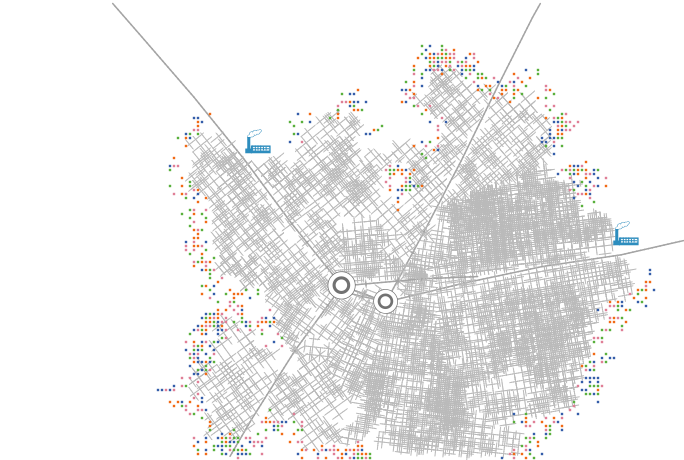
\includegraphics[width=0.33\textwidth]{Figures/PartI/Methodology/Reproducibility/stdView}
\hfill
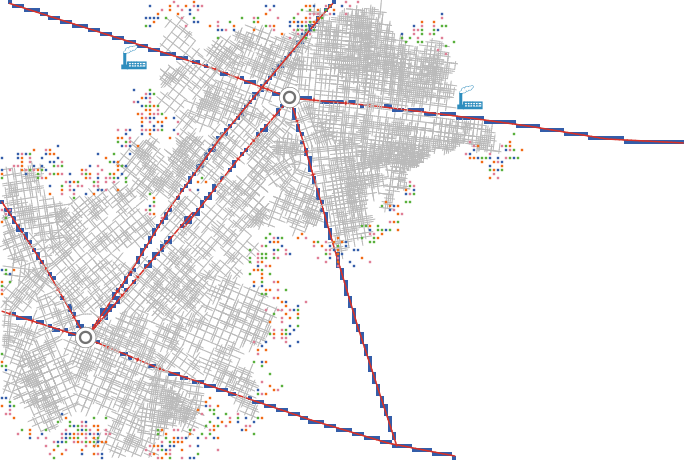
\includegraphics[width=0.33\textwidth]{Figures/PartI/Methodology/Reproducibility/ViewRoads}
\hfill
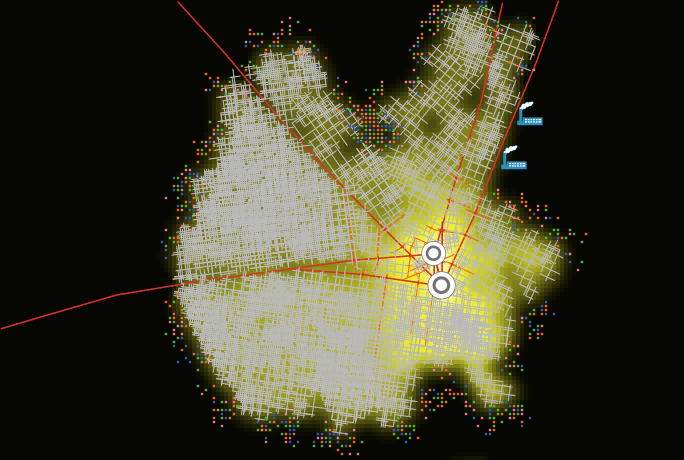
\includegraphics[width=0.33\textwidth]{Figures/PartI/Methodology/Reproducibility/landValues_cityFinished}
\caption[Reproducibility and visualization]{Example of simple improvement in visualization that can help understanding mechanisms implied in the model. \textit{Left : } example of original output ; \textit{Middle : } visualization of main roads (in red) and underlying patches attribution, suggesting possible implementation bias in the use of discretized trace of roads to track their positions ; \textit{Right : }Visualization of land values using a more readable color gradient. This step confirms the hypothesis, through the form of value distribution, that the morphogenesis step is an unnecessary detour to generate a random field for which simple diffusion method should provide similar results, as detailed in the paragraph on implementation.}
\label{fig:example_tij_viz}
\end{figure}




\subsection{On the Need of Exactitude in Model Implementation}

% Barthelemy paper, pb in model description/implementation
%  - test different analyses with possible biaises -

Possible divergences between model description in a paper and the effectively implemented processes may have grave consequences on the reproducibility of science. The road network growth model given in~\cite{barthelemy2008modeling} is one example that we are currently investigating. A strict implementation of model mechanisms provide slightly different results than the one presented in the paper, and as source code is not provided we need to test different hypotheses on possible mechanisms added by the programmer (that seems to be a connexion rule to intersections under a certain distance threshold). Lessons that could be possibly drawn from this examples are 
\begin{itemize}
\item the necessity of providing source code
\item the necessity of providing architecture description along with code (if model description is in a langage too far from architectural specifications) in order to identify possible implementation biaises
\item the necessity of performing and detailing explicitly model explorations, that would in that case have helped to identify the implementation bias.
\end{itemize}

The last point, if first not provided, may ensure a limited risk of scientific falsification as it may be more complicated to fake false exploration results than to effectively explore the model. A joint project currently done is the writing of a false modeling paper in the spirit of~\cite{zilsel2015canular}, in which opposite results to the effective results of a given model are provided, without providing model implementation. A first bunch of test is the acceptance of a clearly non-reproducible paper in diverse journals, possibly with a control on textual elements (using or not ``buzz-words'' associated to the journal, etc.). Depending on results, a second experiment may be tested with providing open source code for model implementation but still with false results, to verify if reviewers effectively try to reproduce results when they pretend to want the code (in reasonable computational power limits of course, HPC being not currently broadly available in Humanities).



\subsection{Perspectives}


Again, reproducibility and transparency is a non-negotiable feature of contemporaneous science, along with Open practices and Open Access. Too much examples (see a very recent one in experimental economics~\cite{camerer2016evaluating}) show in various disciplines the lack of reproducibility of experiments, that is a falsification of previous results or a result in itself. Falsification is a costly practice, and even if necessary~\cite{chavalarias2005nobel}, could be made more efficient through more transparency and direct reproducibility, increase therein the global workflow of science. We develop in parallel of this thesis various tools aimed to ease reproducibility, for which an overview is given in appendix~\ref{app:workflow}.



%----------------------------------------------------------------------------------------

% Section : stochastic framework for urban growth


\newpage

\section{An unified framework for stochastic models of urban growth}

Urban growth modeling fall in the case of tentatives to find self-consistent rules reproducing dynamics of an urban system, and thus in our logic of system morphogenesis. We examine here methodological issues linked to different frameworks of urban growth.

%%%%%%%%%%%%%%%%%%%%
\subsection{Introduction}
%%%%%%%%%%%%%%%%%%%%

Various stochastic models aiming to reproduce population patterns on large temporal and spatial scales (city systems) have been discussed across various fields of the literature, from economics to geography, including models proposed by physicists. We propose here a general framework that allows to include different famous models (in particular Gibrat, Simon and Preferential Attachment model) within an unified vision. It brings first an insight into epistemological debates on the relevance of models. Furthermore, bridges between models lead to the possible transfer of analytical results to some models that are not directly tractable.


%%%%%%%%%%%%%%%%%%%%
%\subsubsection{Context}

Seminal models of urban growth are Simon~\cite{simon1955class} (later generalized as e.g. \cite{haran1973modified}) and Gibrat models. Many examples can be given across disciplines. \cite{benguigui2007dynamic} give an equation-based dynamical model, whereas \cite{gabaix1999zipf} solves a stationary model. \cite{Gabaix20042341} reviews urban growth approaches in economics. A model adapted from evolutive urban theory is solved in~\cite{favaro2011gibrat} and improves Gibrat models. The question of empirical scales at which it is consistent to study urban growth was also tackled in the particular case of France~\cite{bretagnolle2002time}. We stay to a certain level of tractability to include models as essence of our approach is links between models but do not make ontologic assumptions.


%%%%%%%%%%%%%%%%%%%%
%\subsubsection{Notations}



%%%%%%%%%%%%%%%%%%%%
\subsection{Framework}
%%%%%%%%%%%%%%%%%%%%


%%%%%%%%%%%%%%%%%%%%
%\subsubsection{Formulation}

\paragraph{Presentation}
What we propose as a framework can be understood as a meta-model in the sense of~\cite{cottineau2015incremental}, i.e. an modular general modeling process within each model can be understood as a limit case or as a specific case of another model. More simply it should be a diagram of formal relations between models. The ontological aspect is also tackled by embedding the diagram into an ontological state space (which discretization corresponds to the ``bricks'' of the incremental construction of~\cite{cottineau2015incremental}). It constructs a sort of model classification or modelography.

We are still at the stage of different derivations of links between models that are presented hereafter.

%\subsubsection{Models Included}

%The following models are included in our framework. The list is arbitrary but aims to offer a broad view of disciplines concerned

%\subsubsection{Thematic Classification}


%\subsubsection{Framework Formulation}
%Diagram linking various models ; first embedded into time/population plane, cases Discrete/Continous. Other aspects more sparse (ex. spatialization) ; how represent it ?

%%%%%%%%%%%%%%%%%%%%
%\subsection{Models formulation}



%%%%%%%%%%%%%%%%%%%%
\subsection{Derivations}

\subsubsection{Generalization of Preferential Attachment}

\cite{yamasaki2006preferential} give a generalization of the classical Preferential Attachment Network Growth model, as a birth and death model with evolving entities. More precisely, network units gain and lose population (equivalent to links connexions) at fixed probabilities, and new unit can be created at a fixed rate.

\subsubsection{Link between Gibrat and Preferential Attachment Models}

Let consider a strictly positive growth Gibrat model given by $P_i(t)=R_i(t)\cdot P_{i}(t-1)$ with $R_i(t)>1$, $\mu_i(t)=\Eb{R_i(t)}$ and $\sigma_i(t)=\Eb{R_i(t)^2}$. On the other hand, we take a simple preferential attachment, with fixed attachment probability $\lambda \in [0,1]$ and new arrivants number $m>0$. We derive that Gibrat model can be statistically equivalent to a limit of the preferential attachment model, assuming that the moment-generating function of $R_i(t)$ exists. Classical distributions that could be used in that case, e.g. log-normal distribution, are entirely defined by two first moments, making this assumption reasonable.

\begin{lemma}
The limit of a Preferential Attachment model when $\lambda \ll 1$ is a linear-growth Gibrat model, with limit parameters $\mu_i(t)=1+\frac{\lambda}{m\cdot (t-1)}$.
\end{lemma}

\begin{proof}

Starting with first moment, we denote $\bar{P}_i(t)=\Eb{P_i(t)}$. Independence of Gibrat growth rate yields directly $\bar{P}_i(t)=\Eb{R_i(t)}\cdot \bar{P}_i(t-1)$. Starting for the preferential attachment model, we have $\bar{P}_i(t) = \Eb{P_i(t)} = \sum_{k=0}^{+\infty}{k\Pb{P_i(t)=k}}$. But
\[
\{P_i(t)=k\}=\bigcup_{\delta=0}^{\infty}{\left(\{P_i(t-1)=k-\delta\}\cap \{P_i\leftarrow P_i + 1\}^{\delta}\right)}
\]

where the second event corresponds to city $i$ being increased $\delta$ times between $t-1$ and $t$ (note that events are empty for $\delta \geq k$). Thus, being careful on the conditional nature of preferential attachment formulation, stating that $\Pb{\{P_i\leftarrow P_i + 1\} | P_i(t-1)=p} = \lambda\cdot\frac{p}{P(t-1)}$ (total population $P(t)$ assumed deterministic), we obtain

\begin{equation*}
\begin{split}
\Pb{\{P_i\leftarrow P_i + 1\}} & = \sum_{p}{\Pb{\{P_i\leftarrow P_i + 1\} | P_i(t-1)=p}\cdot \Pb{P_i(t-1)=p}}\\
&=\sum_{p}{\lambda\cdot\frac{p}{P(t-1)}\Pb{P_i(t-1)=p}}=\lambda\cdot\frac{\bar{P}_i(t-1)}{P(t-1)}\\
\end{split}
\end{equation*}

It gives therefore, knowing that $P(t-1)=P_0 + m\cdot (t-1)$ and denoting $q=\lambda\cdot\frac{\bar{P}_i(t-1)}{P_0 + m\cdot (t-1)}$

\[
\begin{split}
\bar{P}_i(t) & =\sum_{k=0}^{\infty}{\sum_{\delta=0}^{\infty}{k\cdot \left(\lambda\cdot\frac{\bar{P}_i(t-1)}{P_0 + m\cdot (t-1)}\right)^{\delta}\cdot \Pb{P_i(t-1)=k-\delta}}}\\
& = \sum_{\delta^{\prime}=0}^{\infty}{\sum_{k^{\prime}=0}^{\infty}{\left(k^\prime + \delta^{\prime}\right)\cdot q^{\delta^{\prime}} \cdot \Pb{P_i(t-1)=k^\prime}}}\\
& = \sum_{\delta^{\prime}=0}^{\infty}{q^{\delta^{\prime}}\cdot \left(\delta^{\prime} + \bar{P}_i(t-1)\right)} = \frac{q}{(1-q)^2} + \frac{\bar{P}_i(t-1)}{(1-q)}\\
& = \frac{\bar{P}_i(t-1)}{1-q}\left[1 + \frac{1}{\bar{P}_i(t-1)}\frac{q}{(1-q)}\right]
\end{split}
\]

%& = \bar{P}_i(t-1)\cdot \frac{1}{1-\lambda\cdot\frac{\bar{P}_i(t-1)}{P_0 + m\cdot (t-1)}} \left[1 + \frac{\lambda}{P_0 + m\cdot (t-1)}\cdot \frac{1}{1-\lambda\cdot\frac{\bar{P}_i(t-1)}{P_0 + m\cdot (t-1)}} \right]


As it is not expected to have $\bar{P}_i(t)\ll P(t)$ (fat tail distributions), a limit can be taken only through $\lambda$. Taking $\lambda \ll 1$ yields, as $0 < \bar{P}_i(t)/P(t) < 1$, that $q=\lambda\cdot\frac{\bar{P}_i(t-1)}{P_0 + m\cdot (t-1)} \ll 1$ and thus we can expand in first order of $q$, what gives $\bar{P}_i(t)=\bar{P}_i(t-1)\cdot \left[1 + \left(1+\frac{1}{\bar{P}_i(t-1)}\right)q + o(q))\right]$

\[
\bar{P}_i(t) \simeq \left[1 + \frac{\lambda}{P_0 + m\cdot (t-1)}\right]\cdot \bar{P}_i(t-1)
\]

It means that this limit is equivalent in expectancy to a Gibrat model with $\mu_i(t) = \mu(t)=1 + \frac{\lambda}{P_0 + m\cdot (t-1)}$.

For the second moment, we can do an analog computation. We have still \[\Eb{P_i(t)^2} = \Eb{R_i(t)^2}\cdot \Eb{P_i(t-1)^2}\]
and
\[\Eb{P_i(t)^2}=\sum_{k=0}^{+\infty}{k^2 \Pb{P_i(t)=k}}\] 

We obtain the same way 

\[
\begin{split}
\Eb{P_i(t)^2} & = \sum_{\delta^{\prime}=0}^{\infty}{\sum_{k^{\prime}=0}^{\infty}{\left(k^\prime + \delta^{\prime}\right)^2\cdot q^{\delta^{\prime}} \cdot \Pb{P_i(t-1)=k^\prime}}}\\ 
& = \sum_{\delta^{\prime}=0}^{\infty}{q^{\delta^{\prime}}\cdot \left(\Eb{P_i(t-1)^2}+2\delta^{\prime}\bar{P}_i(t-1) + {\delta^{\prime}}^2\right)}\\
& = \frac{\Eb{P_i(t-1)^2}}{1-q} + \frac{2 q \bar{P}_i(t-1)}{(1-q)^2} + \frac{q(q+1)}{(1-q)^3}\\
& = \frac{\Eb{P_i(t-1)^2}}{1-q}\left[1 + \frac{q}{\Eb{P_i(t-1)^2}}\left(\frac{2\bar{P}_i(t-1)}{1-q} + \frac{(1+q)}{(1-q)^2}\right)\right]
\end{split}
\]



We have therefore an equivalence between the Gibrat model as a continuous formulation of a Preferential Attachment (or Simon model) in a certain limit. \qed

\end{proof}




\subsubsection{Link between Simon and Preferential Attachment}
%\label{subsubsec:gibrat-simon}

A rewriting of Simon model yields a particular case of the generalized preferential attachment, in particular by vanishing death probability.

\subsubsection{Link between Favaro-Pumain and Gibrat}

\cite{favaro2011gibrat} generalizes Gibrat models with innovation propagation dynamics, being therefore a generalization of that model. Theoretically, a process-based model equivalent to the Favaro-pumain should then fill the missing case in model classification at the corresponding discretization. Simpop models do not fill that case as they stay at the scale of city systems, as for Marius models~\cite{cottineau2014evolution}. These must also have their counterparts in discrete microscopic formulation.

\subsubsection{Link between Bettencourt-West and Pumain}

We are considering to study Bettencourt-West model for urban scaling laws \cite{bettencourt2008large} as entering the stochastic urban growth framework as stationary component of a random growth model, but investigation are still ongoing.


\subsubsection{Other Models}

\cite{gabaix1999zipf} develops an economic model giving a Simon equivalent formulation. They in particular find out that in upper tail, proportional growth process occurs. We find the same result as a consequence of the derivation of the link between Gibrat and Preferential attachment models.




%%%%%%%%%%%%%%%%%%%%
%\subsection{Application and Perspectives}
%%%%%%%%%%%%%%%%%%%%







%%%%%%%%%%%%%%%%%%%%
%\subsection{Discussion}
%%%%%%%%%%%%%%%%%%%%

%%%%%%%%%%%%%%%%%%%%
%\subsection*{Conclusion}
%%%%%%%%%%%%%%%%%%%%





%----------------------------------------------------------------------------------------

\newpage


%  section : scaling sensitivity : useful ?


\section{Analytical Sensitivity of Urban Scaling Laws to Spatial Extent}

At the center of evolutive urban theory are hierarchy and associated scaling laws. We begin here an methodological investigation on the sensitivity of scaling laws to city definition.


%%%%%%%%%%%%%%%%%%%%
\subsection{Introduction}



Scaling laws have been shown to be universal of urban systems at many scales and for many indicators. Recent studies question however the consistence of scaling exponents determination, as their value can vary significantly depending on thresholds used to define urban entities on which quantities are integrated, even crossing the qualitative border of linear scaling, from infra-linear to supra-linear scaling. We use a simple theoretical model of spatial distribution of densities and urban functions to show analytically that such behavior can be derived as a consequence of the type of spatial distribution and the method used. Numerical simulation confirm the theoretical results and reveals that results are reasonably independent of spatial kernel used to distribute density.



Scaling laws for urban systems, starting from the well-known rank-size Zipf's law for city size distribution~\cite{gabaix1999zipf}, have been shown to be a recurrent feature of urban systems, at many scales and for many types of indicators. They reside in the empirical constatation that indicators computed on elements of an urban system, that can be cities for system of cities, but also smaller entities at a smaller scale, do fit relatively well a power-law distribution as a function of entity size, i.e. that for entity $i$ with population $P_i$, we have for an integrated quantity $A_i$, the relation $A_i \simeq A_0\cdot \left(\frac{P_i}{P_0}\right)^{\alpha}$. Scaling exponent $\alpha$ can be smaller or greater than 1, leading to infra- or supra-linear effects. Various thematic interpretation of this phenomena have been proposed, typically under the form of processes analysis. The economic literature has produced abundant work on the subject (see~\cite{Gabaix20042341} for a review), but that are generally weakly spatial, thus of poor interest to our approach that deals precisely with spatial organization. Simple economic rules such as energetic equilibria can lead to simple power-laws~\cite{bettencourt2008large} but are difficult to fit empirically. A interesting proposition by Pumain is that they are intrinsically due to the evolutionary character of city systems, where complex emergent interaction between cities generate such global distributions~\cite{pumain2006evolutionary}. Although a tempting parallel can be done with self-organizing biological systems, Pumain insists on the fact that the ergodicity assumption for such systems is not reasonable in the case of geographical systems and that the analogy cannot be exploited~\cite{pumain2012urban}. Other explanations have been proposed at other scales, such as the urban growth model at the mesoscopic scale (city scale) given in~\cite{2014arXiv1401.8200L} that shows that the congestion within transportation networks may be one reason for city shapes and corresponding scaling laws. Note that ``classic'' urban growth models such as Gibrat's model do provide first order approximation of scaling systems, but that interactions between agents have to be incorporated into the model to obtain better fit on real data, such as the Favaro-Pumain model for innovation cycles propagation proposed in~\cite{favaro2011gibrat}, that generalize a Gibrat model and provide better fits on data for French cities.

However, the blind application of scaling exponents computations was recently pointed as misleading in most cases~\cite{louf2014scaling}, confirmed by empirical works such as~\cite{2013arXiv1301.1674A} that showed the variability of computed exponents to the parameters defining urban areas, such as density thresholds. An ongoing work by Cottineau \& \textit{al.} presented at~\cite{cottineau2015scaling}, studies empirically for French Cities the influence of 3 parameters playing a role in city definition, that are a density threshold $\theta$ to delimitate boundaries of an urban area, a number of commuters threshold $\theta_c$ that is the proportion of commuters going to core area over which the unity is considered belonging to the area, and a cut-off parameter $P_c$ under which entities are not taken into account for the linear regression providing the scaling exponent. Remarquable results are that exponents can significantly vary and move from infra-linear to supra-linear when threshold varies. A systematic exploration of parameter space produces phase diagrams of exponents for various quantities. One question raising immediately is how these variation can be explained by the features of spatial distribution of variables. Do they result from intrinsic mechanisms present in the system or can they be explained more simply by the fact that the system is particularly spatialized ? We propose to prove by the tractation of a toy analytical model that even simple distributions can lead to such significant variations in the exponents, along one dimension of parameters (density threshold), directing the response towards the second explanation.
%The rest of the section is organized as follows : we formalize the simple framework used and derive an analytical relation between estimated exponent and density threshold parameter. We then present a numerical implementation of the model that confirms numerically theoretical results, explore other form of kernels that would be less tractable, and study the sensitivity along two parameters. We finally discuss the implications of our results and further work needed.

%%%%%%%%%%%%%%%%%%%%
\subsection{Formalization}
\label{sec:formalization}

We formalize the simple theoretical context in which we will derive the sensitivity of scaling to city definition. Let consider a polycentric city system, which spatial density distributions can be reasonably constructed as the superposition of monocentric fast-decreasing spatial kernels, such as an exponential mixture model~\cite{anas1998urban}. Taking a geographical space as $\mathbb{R}^2$, we take for any $\vec{x}\in\mathbb{R}^2$ the density of population as
\begin{equation}
d(\vec{x}) = \sum_{i=1}^{N}{d_i(\vec{x})} = \sum_{i=1}^{N}{d_i^0\cdot \exp{\left(\frac{-\norm{\vec{x}-\vec{x}_i}}{r_i}\right)}}
\end{equation}

where $r_i$ are spread parameters of kernels, $d_i^0$ densities at origins, $\vec{x}_i$ positions of centers. We furthermore assume the following constraints :

\begin{enumerate}
\item To simplify, cities are monocentric, in the sense that for all $i\neq j$, we have $\norm{\vec{x}_i - \vec{x}_j}\gg r_i$.
\item It allows to impose structural scaling in the urban system by the simple constraint on city populations $P_i$. One can compute by integration that $P_i=2\pi d_i^0 r_i^2$, what gives by injection into the scaling hypothesis $\ln{P_i}=\ln{P_{max}}-\alpha \ln{i}$, the following relation between parameters : $\ln{\left[d_i^0 r_i^2\right]}=K' - \alpha \ln{i}$.
\end{enumerate}

To study scaling relations, we consider a random scalar spatial variable $a(\vec{x})$ representing one aspect of the city, that can be everything but has the dimension of a spatial density, such that the indicator $A(D)=\Eb{\iint_D{a(\vec{x})d\vec{x}}}$ represents the expected quantity of $a$ in area $D$. We make the assumption that $a\in \{0;1\}$ (``counting'' indicator) and that its law is given by $\Pb{a(\vec{x})=1}=f(d(\vec{x}))$. Following the empirical work done in~\cite{cottineau2015scaling}, the integrated indicator on city $i$ as a function of $\theta$ is given by
\[
A_i(\theta) = A(D(\vec{x}_i, \theta))
\]

where $D(\vec{x}_i, \theta)$ is the area centered in $\vec{x}_i$ where $d(\vec{x})>\theta$. Assumption 1 ensures that the area are roughly disjoint circles. We take furthermore a simple amenity such that it follows a local scaling law in the sense that $f(d)=\lambda\cdot d^\beta$. It seems a reasonable assumption since it was shown that many urban variable follow a fractal behavior at the intra-urban scale~\cite{keersmaecker2003using} and that it implies necessarily a power-law distribution~\cite{chen2010characterizing}. We make the additional assumption that $r_i=r_0$ does not depend on $i$, what is reasonable if the urban system is considered from a large scale. This assumption should be relaxed in numerical simulations. The estimated scaling exponent $\alpha(\theta)$ is then the result of the log-regression of $(A_i(\theta))_i$ against $(P_i(\theta))_i$ where $P_i(\theta)=\iint_{D(\vec{x}_i,\theta)}{d}$.


%%%%%%%%%%%%%%%%%%%%
\subsection{Analytical Derivation of Sensitivity}

With above notations, let derive the expression of estimated exponent for quantity $a$ as a function of density threshold parameter $\theta$. The quantity computed for a given city $i$ is, thanks to the monocentric assumption and in a spatial range and a range for $\theta$ such that $\theta \gg \sum_{j\neq i}{d_j(\vec{x})}$, allowing to approximate $d(\vec{x})\simeq d_i(\vec{x})$ on $D(\vec{x}_i,\theta)$, is computed by
\[
\begin{split}
A_i(\theta) & = \lambda\cdot \iint_{D(\vec{x}_i,\theta)}{d^\beta} = 2\pi\lambda {d_i^0}^{\beta} \int_{r=0}^{r_0 \ln{\frac{d_i^0}{\theta}}}{r\exp{\left(-\frac{r\beta}{r_0}\right)}dr}\\
& = \frac{2\pi {d_i^0}^\beta r_0^2}{\beta^2} \left[1 + \beta \ln{\frac{\theta}{d_i^0}\left(\frac{\theta}{d_i^0}\right)^\beta} - \left(\frac{\theta}{d_i^0}\right)^\beta\right]
\end{split}
\]

We obtain in a similar way the expression of $P_i(\theta)$
\[
P_i(\theta) = 2\pi d_i^0 r_0^2 \left[1 + \ln{\left[\frac{\theta}{d_i^0}\right]}\frac{\theta}{d_i^0} - \frac{\theta}{d_i^0}\right]
\]

The Ordinary-Least-Square estimation, solving the problem $\inf_{\alpha,C}\norm{(\ln{A_i(\theta)} - C - \alpha \ln{P_i(\theta)})_i}^2$, gives the value $\alpha(\theta) = \frac{\Covb{(\ln{A_i(\theta)})_i}{(\ln{P_i(\theta)})_i}}{\Varb{(\ln{P_i(\theta)})_i}}$. As we work on city boundaries, threshold is expected to be significantly smaller than center density, i.e. $\theta / d_i^0 \ll 1$. We can develop the expression in the first order of $\theta / d_i^0$ and use the global scaling law for city sizes, what gives $\ln{A_i(\theta)} \simeq K_A - \alpha \ln{i} + (\beta - 1)\ln{d_i^0} + \beta \ln{\frac{\theta}{d_i^0}\left(\frac{\theta}{d_i^0}\right)^\beta} $ and $\ln{P_i(\theta)} = K_P - \alpha \ln{i} + \ln{\left[\frac{\theta}{d_i^0}\right]}\frac{\theta}{d_i^0}$. Developing the covariance and variance gives finally an expression of the scaling exponent as a function of $\theta$, where $k_j,{k_j}'$ are constants obtained in the development :

\begin{equation}
\label{eq:th}
\alpha(\theta) = \frac{k_0 + k_1 \theta + k_2 \theta^\beta + k_3 \theta^{\beta + 1} +  k_4 \theta \ln{\theta} + k_5 \theta^\beta \ln{\theta} + k_6 \theta^\beta (\ln{\theta})^2 + k_7 \theta^{\beta + 1}(\ln{\theta})^2 + k_8 \theta^{\beta + 1}\ln{\theta}}{k_0'+k_1' \ln{\theta} + k_2' \theta \ln{\theta} + k_3' \theta^2 + k_4' \theta^2\ln{\theta} + k_5' \theta^2 (\ln{\theta})^2}
\end{equation}

This rational fraction predicts the evolution of the scaling exponent when the threshold varies. We study numerically its behavior in the next section, among other numerical experiments.


%%%%%%%%%%%%%%%%%%%%
\subsection{Numerical Simulations}

\paragraph{Implementation}

We implement empirically the density model given in section~\ref{sec:formalization}. Centers are successively chosen such that in a given region of space only one kernel dominates in the sense that the sum of other contributions are above a given threshold $\theta_e$. In practice, adapting $N$ to world size allows to respect the monocentric condition. Population are distributed in order to follow the scaling law with fixed $\alpha$ and $r_i$ (arbitrary choice) by computing corresponding $d_i^0$. Technical details of the implementation done in R~\cite{R-Core-Team:2015fk} and using the package \texttt{kernlab} for efficient kernel mixture methods~\cite{Karatzoglou:2004uq} are given as comments in source code\footnote{available at \texttt{https://github.com/JusteRaimbault/CityNetwork/tree/master/Models/Scaling}}. We show in figure~\ref{fig:ex-distrib} example of synthetic density distributions on which the numerical study is conducted. The validation of theoretical results on these experimental mixtures must still be conducted, along with sensitivity tests to random perturbations, influence of kernel type, and two-parameters phase diagram when adding in the computational model functional density distribution and associated cut-off threshold.
%Theoretical result obtained in Eq.~\ref{eq:th} are studied and confronted to emprically computed values for various parameter as shown in Fig.~\ref{fig:th_results}.

\begin{figure}
\centering
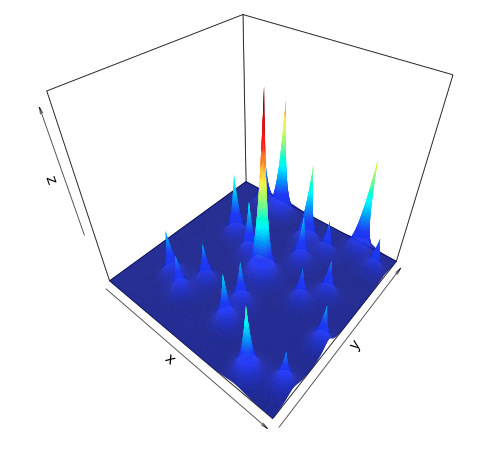
\includegraphics[width=0.4\textwidth]{Figures/PartI/Methodology/Scaling/example_exp_mixture}
\caption[Synthetic density distribution]{Example of a synthetic density distribution obtained with the exponential mixture, with a grid of size $400\times 400$ and parameters $N=20$, $r_0=10$, $P_{max}=200$, $\alpha=0.5$, $\theta_C = 0.01$.}
\label{fig:ex-distrib}
\end{figure}


%\begin{figure}
%\centering
%
%\caption{Validation of theoretical result through numerical simulation.}
%\label{fig:th_results}
%\end{figure}



\paragraph{Random Perturbations}

The simple model used is quite reducing for maximal densities and radius distribution. We aim to proceed to an empirical study of the influence of noise in the system by fixing $d_i^0$ and $r_i$ the following way :
\begin{itemize}
\item $d_i^0$ follows a reversed log-normal distribution with maximal value being a realistic maximal density
\item Radiuses are computed to respect rank-size law and then perturbed by a white noise.
\end{itemize}

%Results shown in Fig.~\ref{fig:random-density} are quantitatively different from previous one, as expected, but the same qualitative behavior is reproduced.


%\begin{figure}
%\centering

%\caption{Variation of exponents with variable origin density and radius.}
%\label{fig:random-density}
%\end{figure}



\paragraph{Kernel Type}

We shall test the influence of the type of spatial kernel used on results. We can test gaussian kernels and quadratic kernels with parameters within reasonable ranges analog to the exponential kernel. %As shown in Fig.~\ref{fig:other-kernels}, we obtain the same qualitative results that is the significant variation of $\alpha(\theta)$ as a function of $\theta$.


%
%\begin{figure}
%\centering

%\caption{Scaling exponents for other kernels.}
%\label{fig:other-kernels}
%\end{figure}

%\paragraph{Two-parameters phase diagram}

%We introduce now a second spatial variable that has also an influence on the definition of urban entities, that is the proportion of actives working in city center, as done on empirical data in~\cite{cottineau2015scaling}. To simplify, it is used only to define urban parameter but assumed as having no influence on the local probability distribution of the amenity which stays the same function of the density. We write 

%\begin{figure}
%\centering

%\caption{Two parameters phase diagram.}
%\label{fig:two-params}
%\end{figure}

%%%%%%%%%%%%%%%%%%%%
%\subsection{Discussion}

%%%%%%%%%%%%%%%%%%%%
%\subsection{Conclusion}








%----------------------------------------------------------------------------------------


\newpage


%  section : synthetic data control - introduces rochebrune paper, feasible correlation space etc, and forthcoming applications ?


\section{Statistical Control on Initial Conditions by Synthetic Data Generation}

\subsection{Context}

When evaluating data-driven models, or even more simple partially data-driven models involving simplified parametrization, an unavoidable issue is the lack of control on ``underlying system parameters'' (what is a ill-defined notion but should be seen in our sense as parameters governing system dynamics). Indeed, a statistics extracted from running the model on enough different datasets can become strongly biased by the presence of confounding in the underlying real data, as it is impossible to know if result is due to processes the model tries to translate or to a hidden structure common to all data.

%Let illustrate the issue with a simple example.

We formalize briefly a proposition of method that would allow to add controls on meta-parameters, in the sense of parameters driving the represented system at a higher temporal and spatial scale, for a model of simulation. We make the hypothesis that such method is valid under constraints of disjonction for scales and/or ontologies between the model of simulation and the domain of meta-parameters.


\subsection{Description}

An advanced knowledge of the behavior of computational models on their parameter space is a necessary condition for deductions of thematic conclusions or their practical application~\cite{banos2013pour}. But the choice of varying parameters is always subjective, as some may be fixed by a real-world parametrization, or other may be interpreted as arbitrarily fixed initial conditions. It raises methodological and epistemological issues for the sensitivity analysis, as the scope of the model may become ill-defined.

Let consider the concrete example of the Schelling Segregation model~\cite{schelling1971dynamic}. One of its crucial features on which the literature has been rather controversial is the influence of the spatial structure of the container on which agents evolve.%~(\textit{Biblio Marion}). 
 The thematic aim of the project developed in~\cite{cottineau2015revisiting} is to clarify this point through a systematic model exploration. A methodological contribution is the construction of a framework allowing the analysis of the sensitivity of models to \emph{meta-parameters}, i.e. to parameters considered as fixed initial conditions (e.g. the spatial structure for the Schelling model), or to parameters of another model generating an initial configuration%, as detailed in Fig.~\ref{} \textit{[insert scheme describing the approach]}, 
 yielding thus a \emph{simple coupling} between models (serial coupling). The benefits of such an approach are various but include for example the knowledge of model behavior in an extended frame, the possibility of statistical control when regressing model outputs, a finer exploration of model derivatives than with a naive approach. Some remarks can be made on the approach :
\begin{itemize}
\item What knowledge are brought by adding the upstream model, rather than for example in the Schelling case exploring a large set of initial geometries ? 

$\rightarrow$ \textit{to obtain a sufficiently large set of initial configuration, one quickly needs a model to generate them ; in that case a quasi-random generation followed by a filtering on morphological constraint will be a morphogenesis model, which parameters are the ones of the generation and the filtering methods. Furthermore, as detailed further, the determination of the derivative of the downstream model is made possible by the coupling and knowledge of the upstream model.}
\item Statistical noise is added by coupling models

$\rightarrow$ \textit{Repetitions needed for convergence are indeed larger as the final expectance has to be determined by repeating on the first times the second model ; but it is exactly the same as exploring directly many configuration, to obtain statistical robustness in that case one must repeat on similar configurations.}

\item Complexity is added by coupling models

% check Varenne citation
$\rightarrow$ \textit{In the sense of Varenne~\cite{varenne2010framework} , coupling is simple and no complexity is thus added.}
\end{itemize}
 
%\paragraph{Context}

%Let $M_{m}$ a stochastic model of simulation, which inputs are to simplify initial conditions $D_0$ and parameters $\vec{\alpha}$, and output $M_{m}\left[\vec{\alpha},D_0\right](t)$ at a given time $t$. We assume that it is partially data-driven in the sense that $D_0$ is supposed to represent a real situation at a given time, and model performance is measured by the distance of its output at final time to the real situation at the corresponding time, i.e. error function is of the form $\norm{\Eb{\vec{g}(M_{m}\left[\vec{\alpha},D_0\right](t_f))}-\vec{g}(D_f)}$ where $\vec{g}$ is a deterministic field corresponding to given indicators.

%\paragraph{Position of the Problem}

%Evaluating the model on real data is rapidly limited in control possibilities, being restricted to the search of datasets allowing natural control groups. Furthermore, statistical behaviors are generally poorly characterized because of the small number of realizations. Working with synthetic data first allows to solve this issue of robustness of statistics, and then gives possibilities of control on some ``meta-parameters'' in the sense described before.




%%%%%%%%%%%%%%%%%%%%
\subsection{Formal Description}

%\subsubsection{Deterministic Formulation}

One has the composition of the derivative along the meta-parameter

\[
\partial_{\alpha}\left[M_u \circ M_d\right] = \left(\partial_{\alpha} M_u \circ M_d \right)\cdot \partial_{\alpha} M_d
\]

$\rightarrow$ \textit{the sensitivity of the downstream model (Schelling) can be determined by studying the serial coupling and the upstream model ; thematic knowledge : sensitivity to an implicit meta-parameter ; and computational gain : generation of controlled differentiates in the ``initial space'' is quasi impossible.}

%\subsubsection{Stochasticity}

The question of stochasticity in simply coupled models causes no additional issue as $\Eb{X}=\Eb{\Eb{X|Y}}$. It naturally multiplies the number of repetition needed for convergence what is the expected behavior.






%----------------------------------------------------------------------------------------

\newpage




\section[Spatio-temporal Correlations]{Linking dynamic and static spatio-temporal correlations under simplified assumptions}

\label{sec:spatiotempcorrs}

Space and Time are both crucial for the study of geographical systems when aiming to understand \emph{processes} (by definition dynamical~\cite{hypergeo}) evolving in a \emph{spatial structure} in the sense of~\cite{dollfus1975some}. Space is more than coordinates for elements of the system, but a dimension in itself that drives interactions and thus system properties. Reading geographical systems from the point of view of \emph{spatio-temporal processes} emphasizes the fact that \emph{space actually matters}. Space and time are closely linked in such processes, and depending on the underlying mechanisms, one can expect to extract useful information from one on the other : in certain cases that we will investigate in this part, it is for example possible to learn about dynamics from static information. Spatio-temporal correlations approaches, linked to spatio-temporal dynamics, are present in very broad fields such as dynamical image processing (including video compression)~\cite{chalidabhongse1997fast,hansen2004accelerated,ke2007spatio}, target tracking~\cite{belouchrani1997direction,vuran2004spatio}, climate science~\cite{cressie1999classes}, Earth sciences~\cite{ma2002spatio}, city systems dynamics~\cite{hernando2015memory,pigozzi1980interurban}, among others.


The capture of neighborhood effects in statistical models is a wisely used practice in spatial statistics, as the technique of Geographically Weighted Regression illustrates~\cite{brunsdon1998geographically}. A possible interpretation among many definitions of spatial autocorrelation~\cite{griffith1992spatial} yields that by estimating a plausible characteristic distance for spatial correlations or auto-correlations, one can isolate independent effects between variables from effects due to neighborhood interactions\footnote{note that the formal link between models of spatial autocorrelation (see e.g. \cite{griffith2012advanced}) is not clear and should be further investigated}. The study of the spatial covariance structure is a cornerstone of advanced spatial statistics that was early formulated~\cite{griffith1980towards}. We propose now to study possible links between spatial and temporal correlations, using spatio-temporal covariance structure to infer information on dynamical processes.


\subsection{Notations}

We consider a multivariate spatio-temporal stochastic process denoted by $\vec{Y}\left[\vec{x},t\right]$. At a given point $\vec{x}_0$ in space, we can define temporal covariance structure by
\[
\mathbf{C}_t (\vec{x}_0) = \Varb{\vec{Y}\left[\vec{x}_0, \cdot\right]}
\]

and spatial covariance structure at fixed time by
\[
\mathbf{C}_x (t) = \Varb{\vec{Y}\left[\cdot, t\right]}
\]

It is clear that these quantities will be in practice first ill-defined because of the difficulty in interpreting such a process by a spatio-temporal random variable, secondly highly non-stationary in space and time. We stay however at a theoretical level to gain structural knowledge, reviewing simple cases in which a formal link can be established.


\subsection{Wave Equation}

In the case of propagating waves, there is an immediate link. Let assume that a wave equation if verified by ``deterministic'' parts of components

\begin{equation}
c^2 \cdot \partial^2_{t} \bar{Y}_i = \Delta \bar{Y}_i
\end{equation}

with $Y_i = \bar{Y}_i + \varepsilon_i$. If errors are uncorrelated and processes are stationary, we have then directly

\begin{equation}
\mathbf{C}_t \left[ \partial^2_t Y_i , \partial^2_t Y_j \right] = \frac{1}{c^2} \cdot\mathbf{C}_x \left[ \Delta Y_i , \Delta Y_j \right]
\end{equation}

This gives us however few insight on real systems as local diffusion, stationary assumptions and uncorrelated noises are far from being verified in empirical situations.

\subsection{Fokker-Planck Equation}

An other interesting approach may when the process verifies a Fokker-Planck equation on probabilities of the state of the system when it is given by its position (diffusion of particles in that case)

\begin{equation}
\partial_t P(x_i,t) = - d \cdot \partial_x P(x_i,t) + \frac{\sigma^2}{2} \partial^2_x P(x_i,t)
\end{equation}

With no cross-correlation terms in the Fokker-Planck equation, covariance between processes vanish. We have finally in that case only a relation between averaged spatial and temporal variances that brings no information to our question.

\subsection{Master Equation}

In the case of a master equation on probabilities of discrete states of the system

\begin{equation}
\partial_t \vec{P} = \mathbb{W} \vec{P}
\end{equation}

we have then for state $i$, $\partial_t P_i = \sum_j W_{ij}P_j$. As this relation is at a fixed time we can average in time to obtain an equation on temporal covariance. It is not clear how to make the link with spatial covariance as these will depend on spatial specification of discrete states. This question is still under investigation.


\subsection{Consistent spatio-temporal sampling}

In a more empirical way, we propose to not assume any contraint of process dynamics but to however investigate how the computation of spatial correlations can inform on temporal correlations. We try to formulate easily verifiable assumptions under which this is possible.

We make the following assumptions on the spatio-temporal stochastic processes $Y_i\left[\vec{x},t\right]$ :
\begin{enumerate}
\item Local spatial autocorrelation is present and bounded by $l_{\rho}$ (in other words the processes are continuous in space) : at any $\vec{x}$ and $t$, $\left|\rho_{\norm{\Delta \vec{x}} < l_{\rho}}\left[Y_i (\vec{x}+\Delta \vec{x},t), Y_i (\vec{x},t) \right]\right| > 0$.
\item Processes are locally parametrized : $Y_i = Y_i\left[\alpha_i\right]$, where $\alpha_i (\vec{x})$ varies with $l_{\alpha}$, with $l_{\alpha} \gg l_{\rho}$.
\item Spatial correlations between processes have a sense at an intermediate scale $l$ such that $l_{\alpha}\gg l \gg l{\rho}$.
\item Processes covariance stationarity times scale as $\sqrt{l}$.
\item Local ergodicity is present at scale $l$ and dynamics are locally chaotic.
\end{enumerate}


Assumptions one to three can be tested empirically and allow to compare spatial correlation estimated on spatial samplings at scale $l$. Assumption four is more delicate as we are precisely constructing this methodology because we have no temporal information on processes. It is however typical of spatial diffusion processes, and population or innovation diffusion should verify this assumption. The last assumption can be tested if feasible space is known, by checking cribbing on image space on the spatial sample. Under these conditions, local spatial sampling is equivalent to temporal sampling and spatial correlation estimators provide estimator of temporal correlations.









%%%%%%%%%%%%%%%%%%%%%%%%%%%%%



%%%%%%%%%%%%%%%%%%%%%%%%%%%%%
% Robustness Discrepancy
% TODO : included in methodological part ?

\newpage

\section[A Discrepancy-based Framework][Un Cadre basé sur la Discrépance]{A Discrepancy-based Framework to Compare Robustness between Multi-Attribute Evaluations}{Un Cadre basé sur la Discrépance pour Comparer la Robustesse des Evaluations Multi-attributs} 

\label{app:sec:robustness}


%----------------------------------------------------------------------------------------



\bpar{
Multi-objective evaluation is a necessary aspect when managing complex systems, as the intrinsic complexity of a system is generally closely linked to the potential number of optimization objectives. However, an evaluation makes no sense without its robustness being given (in the sense of its reliability). Statistical robustness computation methods are highly dependent of underlying statistical models. We propose a formulation of a model-independent framework in the case of integrated aggregated indicators (multi-attribute evaluation), that allows to define a relative measure of robustness taking into account data structure and indicator values. We implement and apply it to a synthetic case of urban systems based on Paris districts geography, and to real data for evaluation of income segregation for Greater Paris metropolitan area. First numerical results show the potentialities of this new method. Furthermore, its relative independence to system type and model may position it as an alternative to classical statistical robustness methods.
}{
Les évaluations multi-objectifs sont un aspect essentiel de la gestion de systèmes complexes, puisque la complexité intrinsèque d'un système est généralement étroitement liée au nombre d'objectifs d'optimisation potentiels. Cependant, une évaluation ne fait pas sens si sa robustesse, au sens de sa fiabilité, n'est pas donnée. Les méthodes statistiques usuelles fournissant une mesure de robustesse sont très dépendantes des modèles sous-jacents. Nous proposons une formulation d'un cadre indépendant du modèle, dans le cas d'indicateurs intégrés et agrégés (évaluation multi-attributs), qui permet de définir une mesure de robustesse relative prenant en compte la structure des données et les valeurs des indicateurs. La méthode est testée sur données urbaines synthétiques associées aux arrondissements de Paris, et à des données réelles de revenus pour l'évaluation de la ségrégation urbaine dans la région métropolitaine du Grand Paris. Les premiers résultats numériques montrent les potentialités de cette nouvelle méthode. De plus, sa relative indépendance au type de système et au modèle pourrait la positionner comme une alternative aux méthodes statistiques classiques d'évaluation de la robustesse.
}


%%%%%%%%%%%%%%%%
%% Intro
%%%%%%%%%%%%%%%%
\subsection{Introduction}{Introduction}

%%%%%%%%%%%%%%%%
\subsubsection{General Context}{Contexte Général}


\bpar{
Multi-objective problems are organically linked to the complexity of underlying systems. Indeed, either in the field of \emph{Complex Industrial Systems}, in the sense of engineered systems, where construction of Systems of Systems (SoS) by coupling and integration often leads to contradictory objectives~\cite{marler2004survey}, or in the field of \emph{Natural Complex Systems}, in the sense of non engineered physical, biological or social systems that exhibit emergence and self-organization properties, where objectives can e.g. be the result of heterogeneous interacting agents (see~\cite{newman2011complex} for a large survey of systems concerned by this approach), multi-objective optimization can be explicitly introduced to study or design the system but is often already implicitly ruling the internal mechanisms of the system. The case of socio-technical Complex Systems is particularly interesting as, following~\cite{haken2003face}, they can be seen as hybrid systems embedding social agents into ``technical artifacts'' (sometimes to an unexpected degree creating what \noun{Picon} describes as \emph{cyborgs}~\cite{picon2013smart}), and thus cumulate propensity to be at the origin of multi-objective issues\footnote{We design by \emph{Multi-Objective Evaluation} all practices including the computation of multiple indicators of a system (it can be multi-objective optimization for system design, multi-objective evaluation of an existing system, multi-attribute evaluation ; our particular framework corresponds to the last case).}. The new notion of \emph{eco-districts}~\cite{souami2012ecoquartiers} is a typical example where sustainability implies contradictory objectives. The example of transportation systems, which conception shifted during the second half of the 20th century from cost-benefit analysis to multi-criteria decision-making, is also typical of such systems~\cite{bavoux2005geographie}. Geographical system are now well studied from such a point of view in particular thanks to the integration of multi-objective frameworks within Geographical Information Systems~\cite{carver1991integrating}. As for the micro-case of eco-districts, meso and macro urban planning and design may be made sustainable through indicators evaluation~\cite{jegou2012evaluation}.
}{
Les problèmes multi-objectifs sont organiquement liés à la complexité des systèmes sous-jacents. En effet, que ce soit dans le champ des \emph{Systèmes Complexes Industriels}, dans le sens de systèmes conçus par ingénierie, où la construction de Systèmes de Systèmes (SoS) par couplage et intégration induit souvent des objectifs contradictoires~\cite{marler2004survey}, ou dans le champ des \emph{Systèmes Complexes Naturels}, au sens de systèmes non désignés, physiques, biologiques ou sociaux, qui présentent des propriétés d'émergence et d'auto-organisation, pour lesquels les objectifs peuvent e.g. être le résultat de l'interaction d'agents hétérogènes (voir~\cite{newman2011complex} pour une revue étendue des types de systèmes concernés par cette approche), l'optimisation multi-objectifs peut être explicitement introduite pour étudier ou désigner le système, mais régit généralement déjà implicitement les mécanismes internes du système. Le cas des Systèmes Complexes Sociaux-techniques est particulièrement intéressant puisque selon Haken~\cite{haken2003face}, ils peuvent être vus comme des systèmes hybrides embarquant des agents sociaux dans des ``artefacts techniques'' (parfois jusqu'à un niveau inattendu, créant ce que \noun{Picon} décrit comme \emph{cyborgs}~\cite{picon2013smart}), et cumulent ainsi la potentialité d'être à l'origine de problèmes multi-objectifs\footnote{Nous désignons ici par \emph{Evaluation Multi-objectifs} toutes les pratiques incluant le calcul de multiples indicateurs d'un système (il peut s'agir d'optimisation multi-objectif pour un design de système, une évaluation multi-objectif d'un système existant, une évaluation multi-attributs ; notre cadre particulier correspondra au dernier cas).}. La notion récente d'\emph{éco-quartier}~\cite{souami2012ecoquartiers} est un exemple typique pour lequel la durabilité implique des objectifs contradictoires. L'exemple des systèmes de transport, dont la conception a glissé durant la seconde moitié du 20ème siècle d'analyses coût-bénéfices à la price de décision multi-critères, est également typique de tels systèmes~\cite{bavoux2005geographie}. Les systèmes géographiques sont à présent bien étudiés d'un tel point de vue, en particulier grâce à l'intégration des cadres multi-objectifs au sein des Systèmes d'Information Géographiques~\cite{carver1991integrating}. Comme dans le cas microscopique des éco-quartiers, la planification et le design urbains mésoscopiques et macroscopiques peuvent être rendus durables grâce aux évaluations par indicateurs~\cite{jegou2012evaluation}.
}



\bpar{
A crucial aspect of an evaluation is a certain notion of its reliability, that we call here \emph{robustness}. % Various definitions of robustness are possible in different frames, and it will have a precise definition in our framework.
Statistics naturally include this notion since the construction and estimation of statistical models give diverse indicators of the consistence of results~\cite{launer2014robustness}. The first example that comes to mind is the application of the law of large numbers to obtain the \emph{p-value} of a model fit, that can be interpreted as a confidence measure of estimates. Besides, confidence intervals and \emph{beta-power} are other important indicators of statistical robustness. Bayesian inference provide also measures of robustness when distribution of parameters are sequentially estimated. Concerning multi-objective optimization, in particular through heuristic algorithms (for example genetic algorithms, or operational research solvers), the notion of robustness of a solution concerns more the stability of the solution on the phase space of the corresponding dynamical system. Recent progresses have been done towards unified formulation of robustness for a multi-objective optimization problem, such as~\cite{deb2006introducing} where robust Pareto-front as defined as solutions that are insensitive to small perturbations. In~\cite{1688537}, the notion of degree of robustness is introduced, formalized as a sort of continuity of other solutions in successive neighborhood of a solution.
}{
Un aspect crucial de l'évaluation est une certaine notion de sa fiabilité, que nous nommerons ici \emph{robustesse}. Les méthodes statistiques incluent naturellement cette notion puisque la construction et l'estimation de modèles statistiques donne divers indicateurs de la consistence des résultats~\cite{launer2014robustness}. Le premier exemple venant à l'esprit est l'application de la loi des grands nombres pour obtenir la \emph{p-valeur} d'une estimation de modèle, qui peut être interprété comme une mesure de confiance en les valeurs estimées. D'autre part, les intervalles de confiance et le  \emph{beta-power} sont d'autres indicateurs importants de robustesse statistique. L'inférence bayésienne fournit également des mesures de robustesse quand la distribution des paramètres est estimée de manière séquentielle. Concernant les optimisations multi-objectifs, en particulier par des algorithmes heuristiques (comme par exemple les algorithmes génétiques, ou les solveurs de recherche opérationelle), la notion de robustesse d'une solution consiste plus en la stabilité de la solution dans l'espace des phases du système dynamique correspondant. Des progrès récents ont été faits vers une formulation unifiée de la robustesse pour les problèmes d'optimisation multi-objectifs, comme dans~\cite{deb2006introducing} où les fronts de Pareto robustes sont définis comme des solutions insensibles aux petites perturbations. Dans~\cite{1688537}, la notion de degré de robustesse est introduite, formalisée comme une sorte de continuité des autres solutions dans des voisinages successifs d'une solution.
}


\bpar{
However, there still lack generic methods to estimate robustness of an evaluation that would be model-independent, i.e. that would be extracted from data structure and indicators but that would not depend on the method used. Some advantages could be for example an \emph{a priori} estimation of potential robustness of an evaluation and thus to decide if the evaluation is worth doing. We propose here a framework answering this issue in the particular case of Multi-attribute evaluations, i.e. when the problem is made unidimensional by objectives aggregation. It is data-driven and not model-driven in the sense that robustness estimation does not depend on how indicators are computed, as soon as they respect some assumptions that will be detailed in the following.
}{
Cependant, il n'existe pas de méthode générique qui permettrait une évaluation de la robustesse de façon indépendante au modèle, i.e. qui serait extraite de la structure des données et des indicateurs mais ne dépendrait pas de la méthode utilisée. Un avantage serait par exemple une estimation \emph{a priori} de la robustesse potentielle d'une évaluation et de décider ainsi si elle vaut la peine d'être faite. Nous proposons un cadre répondant à cette contrainte dans le cas particulier des évaluations multi-attributs, i.e. quand le problème est rendu unidimensionnel par agrégation des objectifs. Il est basé sur les données et non sur les modèles, au sens ou l'estimation de la robustesse ne dépendra pas de la manière dont les indicateurs sont calculés, tant qu'ils respectent certaines hypothèses détaillées par la suite.
}



%%%%%%%%%%%%%%%%
\subsubsection{Proposed Approach}{Approche Proposée}



\paragraph{Objectives as Spatial Integrals}{Objectifs comme intégrales spatiales}


\bpar{
We assume that objectives can be expressed as spatial integrals, so it should apply to any territorial system and our application cases are urban systems. It is not that restrictive in terms of possible indicators if one uses suitable variables and integrated kernels : in a way analog to the method of geographically weighted regression~\cite{brunsdon1998geographically}, any spatial variable can be integrated against regular kernels of variable size and the result will be a spatial aggregation which sense depends on kernel size. The example we use in the following such as conditional means or sums suit well the assumption. Even an already spatially aggregated indicator can be interpreted as a spatial indicator by using a Dirac distribution on the centroid of the corresponding area.
}{
Nous supposons que les objectifs peuvent être exprimés comme intégrales spatiales, ce qui devrait s'appliquer à tout système territorial, et nos cas d'application sont des systèmes urbains. Ce n'est pas si restrictif en terme d'indicateurs possibles si l'on utilise les bonnes variables et noyaux intégrés : de façon analogue à la méthode de Regression Géographique Pondérée~\cite{brunsdon1998geographically}, toute variable spatiale peut être intégrée contre des noyaux réguliers de taille variable et le résultats sera une agrégation spatiale dont la signification dépendra de l'étendue du noyau. Les exemples utilisés par la suite comme des moyennes conditionnelles ou des sommes vérifient parfaitement cette hypothèse. Même un indicateur déjà agrégé dans l'espace peut être interprété comme une intégrale spatiale en utilisant une distribution de Dirac au centroïde de la zone correspondante. 
}



\paragraph{Linearly Aggregated Objectives}{Objectifs agrégés linéairement}

\bpar{
A second assumption we make is that the multi-objective evaluation is done through linear aggregation of objectives, i.e. that we are tackling a multi-attribute optimization problem. If $(q_i(\vec{x}))_i$ are values of objectives functions, then weights $(w_i)_i$ are defined in order to build the aggregated decision-making function $q(\vec{x})=\sum_i{w_i q_i(\vec{x})}$, which value determines then the performance of the solution. It is analog to aggregated utility techniques in economics and is used in many fields. The subtlety lies in the choice of weights, i.e. the shape of the projection function, and various approaches have been developed to find weights depending on the nature of the problem. Recent work~\cite{dobbie2013robustness} proposed to compare robustness of different aggregation techniques through sensitivity analysis, performed by Monte-Carlo simulations on synthetic data. Distribution of biases where obtained for various techniques and some showed to perform significantly better than others. Robustness assessment still depended on models used in that work.
}{
Une seconde hypothèse que nous faisons est que l'évaluation multi-objectifs est effectuée par agrégation linéaire des objectif, c'est à dire qu'on se place dans le cadre d'un problème d'optimisation multi-attributs. Si $(q_i(\vec{x}))_i$ sont les valeurs des fonctions objectifs, on définit alors des poids $(w_i)_i$ afin de construire la fonction de prise de décision $q(\vec{x})=\sum_i{w_i q_i(\vec{x})}$, dont la valeur détermine ensuite la performance d'une solution. Cette approche est analogue aux utilités agrégées en économie et est utilisée dans de nombreux domaines. La subtilité réside dans le choix des poids, i.e. de la forme de la fonction de projection, et différentes solutions ont été dévelopées pour obtenir des poids selon la nature du problème. Récemment, \cite{dobbie2013robustness} a proposé de comparer la robustesse des différentes techniques d'agrégation par une analyse de sensibilité, effectuée par simulations de Monte-Carlo pour produire des données synthétiques, ce qui permet d'obtenir la distribution des biais pour les différentes techniques, certaines étant significativement plus performantes que d'autres. Toutefois, la quantification de la robustesse dépend toujours des modèles utilisés dans ce travail.
}


\bigskip


\bpar{
The rest of the paper is organized as follows : section 2 describes intuitively and mathematically the proposed framework ; section 3 then details implementation, data collection for case studies and numerical results for an artificial intra-urban case and a metropolitan real case ; section 4 finally discuss limitations and potentialities of the method.
}{
Le reste de cette monographie est organisé de la façon suivante : la section 2 décrit intuitivement puis mathématiquement le cadre proposé ; la section 3 détaille ensuite l'implémentation, la collecte des données pour les cas d'étude et les résultats numériques pour une évaluation intra-urbaine synthétique et un cas réel métropolitain ; la section 4 discute finalement les limitations et les potentialités de la méthode.
}




%%%%%%%%%%%%%%%%
%% Framework Description
%%%%%%%%%%%%%%%%
\subsection{Framework Description}{Description du Cadre}


%%%%%%%%%%%%%%%%
\subsubsection{Intuitive Description}{Description Intuitive}


\bpar{
We describe now the abstract framework allowing theoretically to compare robustnesses of evaluations of two different urban systems. Our framework is a generalization of an empirical method proposed in~\cite{ecodistrictReport} besides a more general benchmarking study on indicator sense and relevance in a sustainability context. Intuitively, it relies on empirical base resulting from the following axioms :
\begin{itemize}
\item Urban systems can be seen from the information available, i.e. raw data describing the system. As a data-driven approach, this raw data is the basis of our framework and robustness will be determined by its structure.
\item From data are computed indicators (objective functions). We assume that a choice of indicators is an intention to translate particular aspects of the system, i.e. to capture a realization of an ``urban fact'' (\emph{fait urbain}) in the sense of \noun{Mangin}~\cite{mangin1999projet} - a sort of stylized fact in terms of processes and mechanisms, having various realizations on spatially distinct systems, depending on each precise context.
\item Given many systems and associated indicators, a common space can be built to compare them. In that space, data represents more or less well real systems, depending e.g. on initial scale, precision of data, missing data. We precisely propose to capture that through the notion of point cloud discrepancy, which is a mathematical tool coming from sampling theory expressing how a dataset is distributed in the space it is embedded in~\cite{dick2010digital}. %Coupling discrepancies with appropriate weights depending on indicator importance allows to introduce a relative ratio of robustness between two evaluations.
\end{itemize}


Synthesizing these requirements, we propose a notion of \emph{Robustness} of an evaluation that captures both, by combining data reliability with relative importance,
\begin{enumerate}
\item \emph{Missing Data} : an evaluation based on more refined datasets will naturally be more robust.
\item \emph{Indicator importance} : indicators with more relative influence will weight more on the total robustness.
\end{enumerate}
}{
Nous décrivons à présent le cadre proposé pour permettre théoriquement de comparer la robustesse d'évaluation de deux systèmes urbains différents. Ce cadre est une généralisation d'une méthode empirique proposée dans~\cite{ecodistrictReport} pour accompagner une étude dans un autre contexte effectuant une comparaison du sens et de la pertinence des indicateurs dans un contexte de durabilité. Intuitivement, la base empirique se base sur les principes suivants :

\begin{itemize}
\item Les systèmes urbains peuvent être vus selon l'information disponible, i.e. les données brutes décrivant le système. Dans une approche basée sur les données, celles-ci sont la base de notre cadre et la robustesse sera déterminée par leur structure.
\item A partir des données sont capturés des indicateurs (fonctions objectifs). Nous supposons qu'un choix d'indicateurs est une intention particulière de traduire des aspects particuliers du système, i.e. de capturer une réalisation d'un ``fait urbain'' au sens de \noun{Mangin}~\cite{mangin1999projet} - une sorte de fait stylisé en terme de processus et de mécanismes, ayant différentes réalisations sur des systèmes distincts dans l'espace, dépendant de chaque contexte géographique précis.
\item Etant donné plusieurs systèmes et indicateurs associés, un espace commun peut être construit pour les comparer. Dans cet espace, les données représentent plus ou moins bien le système réel, c'est à dire qu'elles sont imprécises en fonction de l'échelle initiale, de la précision effective des données. Nous proposons de capturer exactement ces différents aspects au travers de la notion de discrépance d'un nuage de points, qui est un outil mathématique provenant des théories d'échantillonnage, permettant d'exprimer la façon dont un jeu de données rempli l'espace dans lequel il s'insère~\cite{dick2010digital}.
\end{itemize}

Synthétisant ces contraintes, nous proposons une notion de \emph{Robustesse} d'une évaluation qui capture à la fois, en combinant la fiabilité des données à l'importance relative des indicateurs,


\begin{enumerate}
\item \emph{Données manquantes} : une évaluation se basant sur des jeux de données plus raffinés sera naturellement plus robuste.
\item \emph{Importance des indicateurs} : les indicateurs avec plus d'importance relative pèseront plus dans la robustesse totale.
\end{enumerate}
}




%%%%%%%%%%%%%%%%
\subsubsection{Formal Description}{Description Formelle}


%%%%%%%%%%%%%%%%
\paragraph{Indicators}{Indicateurs}


\bpar{
Let $(S_{i})_{1\leq i\leq N}$ be a finite number of geographically disjoints territorial systems, that we assume described through raw data and intermediate indicators, yielding $S_{i}=(\mathbf{X}_{i},\mathbf{Y}_{i})\in\mathcal{X}_{i}\times\mathcal{Y}_{i}$ with $\mathcal{X}_{i}=\prod_{k}\mathcal{X}_{i,k}$ such that each subspace contain real matrices : $\mathcal{X}_{i,k}=\mathbb{R}^{n_{i,k}^{X}p_{i,k}^{X}}$ (the same holding for $\mathcal{Y}_{i}$). We also define an ontological index function $I_{X}(i,k)$ (resp. $I_{Y}(i,k)$) taking integer values which coincide if and only if the two variables have the same ontology in the sense of~\cite{livet2010}, i.e. they are supposed to represent the same real object. We distinguish ``raw data'' $\mathbf{X}_{i}$ from which indicators are computed via explicit deterministic functions, from ``intermediate indicators'' $\mathbf{Y}_{i}$ that are already integrated and can be e.g. outputs of elaborated models simulating some aspects of the urban system. We define the partial characteristic space of the ``urban fact'' by 

\begin{equation}
%\begin{split}
%(\mathcal{X},\mathcal{Y}) & \underset{def}{=} \left(\prod\tilde{\mathcal{X}}_{c}\right)\times\left(\prod\tilde{\mathcal{Y}}_{c}\right)\\
%& =  \left(\prod_{\mathcal{X}_{i,k}\in\mathcal{D}_{\mathcal{X}}}\mathbb{R}^{p_{i,k}^{X}}\right)\times\left(\prod_{\mathcal{Y}_{i,k}\in\mathcal{D}_{\mathcal{Y}}}\mathbb{R}^{p_{i,k}^{Y}}\right)
%\end{split}
(\mathcal{X},\mathcal{Y}) \underset{def}{=} \left(\prod\tilde{\mathcal{X}}_{c}\right)\times\left(\prod\tilde{\mathcal{Y}}_{c}\right) = \left(\prod_{\mathcal{X}_{i,k}\in\mathcal{D}_{\mathcal{X}}}\mathbb{R}^{p_{i,k}^{X}}\right)\times\left(\prod_{\mathcal{Y}_{i,k}\in\mathcal{D}_{\mathcal{Y}}}\mathbb{R}^{p_{i,k}^{Y}}\right)
\end{equation}


with $\mathcal{D}_{\mathcal{X}}=\{\mathcal{X}_{i,k}|I(i,k)\textrm{ distincts},n_{i,k}^{X}\mbox{ maximal}\}$
(the same holding for $\mathcal{Y}_{i}$). It is indeed the abstract space on which indicators are integrated. The indices $c$ introduced as a definition here correspond to different indicators across all systems. This space is the minimal space common to all systems allowing a common definition for indicators on each.
}{
Soit $(S_{i})_{1\leq i\leq N}$ un nombre fini de systèmes territoriaux géographiquement disjoints, \comment{Q pourquoi nécessaire des les avoir spatially disjoints, could be different indicators on the same area ? maybe makes less sense ? missing point for comparability ?}
que nous supposons décrits par les données brutes et des indicateurs intermédiaires, donnés par $S_{i}=(\mathbf{X}_{i},\mathbf{Y}_{i})\in\mathcal{X}_{i}\times\mathcal{Y}_{i}$ avec $\mathcal{X}_{i}=\prod_{k}\mathcal{X}_{i,k}$ tel que chaque sous-espace contient des matrices réelles : $\mathcal{X}_{i,k}=\mathbb{R}^{n_{i,k}^{X}p_{i,k}^{X}}$ (de la même façon pour $\mathcal{Y}_{i}$). Nous définissons également une fonction d'indice ontologique $I_{X}(i,k)$ (resp. $I_{Y}(i,k)$) prenant des valeurs entières qui coincident si et seulement si les deux variables ont même ontologie au sens de~\cite{livet2010}, c'est à dire qu'elles sont supposées représenter le même objet réel. On distingue les ``données brutes'' $\mathbf{X}_{i}$ à partir desquelles les indicateurs sont calculés généralement par des fonctions déterministes explicites, \comment{not that free on the computation here !}
 des ``indicateurs intermédiaires'' $\mathbf{Y}_{i}$ qui sont déjà intégrés et peuvent être par exemple les sorties de modèles élaborés simulant certains aspects du système urbain. Nous définissons l'espace caractéristique du ``fait urbain'' par


\begin{equation}
(\mathcal{X},\mathcal{Y}) \underset{def}{=} \left(\prod\tilde{\mathcal{X}}_{c}\right)\times\left(\prod\tilde{\mathcal{Y}}_{c}\right) = \left(\prod_{\mathcal{X}_{i,k}\in\mathcal{D}_{\mathcal{X}}}\mathbb{R}^{p_{i,k}^{X}}\right)\times\left(\prod_{\mathcal{Y}_{i,k}\in\mathcal{D}_{\mathcal{Y}}}\mathbb{R}^{p_{i,k}^{Y}}\right)
\end{equation}

avec $\mathcal{D}_{\mathcal{X}}=\{\mathcal{X}_{i,k}|I(i,k)\textrm{ distincts},n_{i,k}^{X}\mbox{ maximal}\}$
(de même pour $\mathcal{Y}_{i}$). Il s'agit en fait de l'espace abstrait sur lequel les indicateurs sont intégrés. Les indices $c$ introduit par définition correspondent aux différents indicateurs au sein des différents systèmes. Cette espace est l'espace minimal commun à tous les systèmes permettant une définition commune des indicateurs pour tous.
}



\bpar{
Let $\mathbf{X}_{i,c}$ be the data canonically projected in the corresponding subspace, well defined for all $i$ and all $c$. We make the key assumption that all indicators are computed by integration against a certain kernel, i.e. that for all $c$, there exists $H_{c}$ space of real-valued functions on $(\tilde{\mathcal{X}}_{c},\tilde{\mathcal{Y}}_{c})$, such that for all $h\in H_{c}$ :
\begin{enumerate}
\item $h$ is ``enough'' regular (tempered distributions e.g.)
\item $q_c=\int_{(\tilde{\mathcal{X}}_{c},\tilde{\mathcal{Y}}_{c})}h$ is a function describing the ``urban fact'' (the indicator in itself)
\end{enumerate}

Typical concrete example of kernels can be :

\begin{itemize}
\item A mean of rows of $\mathbf{X}_{i,c}$ is computed with $h(x)=x\cdot f_{i,c}(x)$ where $f_{i,c}$ is the density of the distribution of the assumed underlying variable.
\item A rate of elements respecting a given condition $C$, $h(x)=f_{i,c}(x)\chi_{C(x)}$ 
\item For already aggregated variables $\mathbf{Y}$, a Dirac distribution allows to express them also as a kernel integral. 
\end{itemize}
}{
Soit $\mathbf{X}_{i,c}$ les données projetées canoniquement sur le sous-espace correspondant, bien définies pour tout $i$ et tout $c$. Nous faisons donc l'hypothèse clé que tous les indicateurs sont calculés par intégration contre un noyau donné, i.e. pour tout $c$ il existe $H_{c}$ espace de fonctions à valeurs réelles sur $(\tilde{\mathcal{X}}_{c},\tilde{\mathcal{Y}}_{c})$, tel que pour tout $h\in H_{c}$ : 

\begin{enumerate}
\item $h$ est ``suffisamment'' régulière (distribution tempérée par exemple)
\item $q_c=\int_{(\tilde{\mathcal{X}}_{c},\tilde{\mathcal{Y}}_{c})}h$ est une fonction décrivant le ``fait urbain'' (l'indicateur en lui-même)
\end{enumerate}

Des exemples typiques de noyaux peuvent être :


\begin{itemize}
\item Une moyenne des lignes de $\mathbf{X}_{i,c}$ est calculée par $h(x)=x\cdot f_{i,c}(x)$ où $f_{i,c}$ est la densité de la distribution de la variable sous-jacente.
\item Un taux d'éléments du jeu de données respectant une condition donnée $C$, $h(x)=f_{i,c}(x)\chi_{C(x)}$.
\item Pour des variables déjà agrégées $\mathbf{Y}$, une distribution de Dirac permet des les exprimer également comme des intégrales de noyaux.
\end{itemize}

}


%%%%%%%%%%%%%%%%
\paragraph{Aggregation}{Agrégation}


\bpar{
Weighting objectives in multi-attribute decision-making is indeed the crucial point of the processes, and numerous methods are available (see~\cite{wang2009review} for a review for the particular case of sustainable energy management). Let define weights for the linear aggregation. We assume the indicators normalized, i.e. $q_c \in [0,1]$, for a more simple construction of relative weights. For $i,c$ and $h_{c}\in H_{c}$ given, the weight $w_{i,c}$ is simply constituted by the relative importance of the indicator $w_{i,c}^{L}=\frac{\hat{q}_{i,c}}{\sum_{c}\hat{q}_{i,c}}$ where $\hat{q}_{i,c}$ is an estimator of $q_{c}$ for data $\mathbf{X}_{i,c}$ (i.e. the effectively calculated value). Note that this step can be extended to any sets of weight attributions, by taking for example $\tilde{w}_{i,c} = w_{i,c} \cdot w'_{i,c}$ if $\mathbf{w}'$ are the weights attributed by the decision-maker. We focus here on the relative influence of attributes and thus choose this simple form for weights.
}{
La détermination des poids est en fait le point crucial des processus de prise de décision multi-attributs, et de nombreuses méthodes sont disponibles (voir~\cite{wang2009review} pour une revue dans le cas particulier de la gestion de l'énergie durable). Définissons les poids pour l'agrégation linéaire. Nous supposons les indicateurs normalisés, i.e. $q_c \in [0,1]$, pour une construction plus simple des poids relatifs. \comment{indeed $h_c \in [0,1]$ is the right assumption}
Pour $i,c$ et $h_{c}\in H_{c}$ donnés, le poids $w_{i,c}$ est simplement constitué par l'importance relative de l'indicateur $w_{i,c}^{L}=\frac{\hat{q}_{i,c}}{\sum_{c}\hat{q}_{i,c}}$ où $\hat{q}_{i,c}$ est un estimateur de $q_{c}$ pour les données $\mathbf{X}_{i,c}$ (i.e. la valeur calculée effectivement). On peut noter que cette étape n'est pas contraignante et que cela peut être étendu à tout ensemble d'attribution de poids, en prenant par exemple $\tilde{w}_{i,c} = w_{i,c} \cdot w'_{i,c}$ si $\mathbf{w}'$ sont les poids fixés par le preneur de décisions. Nous nous concentrons sur l'influence relative des attributs et pour cela choisissons cette forme simple pour les poids. 
}










%%%%%%%%%%%%%%%%
\paragraph{Robustness Estimation}{Estimation de la Robustesse}


\bpar{
The scene is now set up to be able to estimate the robustness of the evaluation done through the aggregated function. Therefore, we apply an integral approximation method similar to methods introduced in~\cite{varet2010developpement}, since the integrated form of indicators indeed brings the benefits of such powerful theoretical results. Let $\mathbf{X}_{i,c}=(\vec{X}_{i,c,l})_{1\leq l\leq n_{i,c}}$ and $D_{i,c}=Disc_{\tilde{\mathcal{X}}_{c},L^2}(\mathbf{X}_{i,c})$ the discrepancy of data points cloud\footnote{The discrepancy is defined as the $L2$-norm of local discrepancy which is for normalized data points $\mathbf{X}=(x_{ij})\in \left[0,1\right]^d$, a function of $\mathbf{t}\in \left[0,1\right]^d$ comparing the number of points falling in the corresponding hypercube with its volume, by $disc(\mathbf{t}) = \frac{1}{n}\sum_i \mathbbm{1}_{\prod_j x_{ij}<t_j} - \prod_j t_j$. It is a measure of how the point cloud covers the space.}~\cite{niederreiter1972discrepancy}. With $h\in H_{c}$, we have the upper bound on the integral approximation error

\[
\left\Vert \int h_{c}-\frac{1}{n_{i,c}}\sum_{l}h_{c}(\vec{X}_{i,c,l})\right\Vert \leq K\cdot\left|\left|\left|h_{c}\right|\right|\right|\cdot D_{i,c}
\]

where $K$ is a constant independent of data points and objective function. It directly yields

\[
\left\Vert \int\sum w_{i,c}h_{c}-\frac{1}{n_{i,c}}\sum_{l}w_{i,c}h_{c}(\vec{X}_{i,c,l})\right\Vert \leq K\sum_{c}\left|w_{i,c}\right|\left|\left|\left|h_{c}\right|\right|\right|\cdot D_{i,c}
\]

Assuming the error reasonably realized (``worst case'' scenario for knowledge of the theoretical value of aggregated function), we take this upper bound as an approximation of its magnitude. Furthermore, taking normalized indicators implies $\left|\left|\left|h_c\right|\right|\right| = 1$. We propose then to compare error bounds between two evaluations. They depend only on data distribution (equivalent to \emph{statistical robustness}) and on indicators chosen (sort of \emph{ontological robustness}, i.e. do the indicators have a real sense in the chosen context and do their values make sense), and are a way to combine these two type of robustnesses into a single value.
}{
La scène est à présent apprêtée pour construire une estimation de la robustesse d'une évaluation faite par la fonction d'agrégation. Pour cela, nous appliquons un théorème d'approximation d'intégrale similaire au méthodes introduites dans~\cite{varet2010developpement}, puisque la forme intégrée des indicateurs permet justement de bénéficier de tels résultats théoriquement puissant. Soit $\mathbf{X}_{i,c}=(\vec{X}_{i,c,l})_{1\leq l\leq n_{i,c}}$ et $D_{i,c}=Disc_{\tilde{\mathcal{X}}_{c},L^2}(\mathbf{X}_{i,c})$ le discrépance du jeu de données\footnote{La discrépance est définie comme la norme-$L2$ de la discrépance locale qui est pour des points de données normalisés $\mathbf{X}=(x_{ij})\in \left[0,1\right]^d$, une fonction de $\mathbf{t}\in \left[0,1\right]^d$ comparant le nombre de points compris dans le volume de l'hypercube correspondant, donné par $disc(\mathbf{t}) = \frac{1}{n}\sum_i \mathbbm{1}_{\prod_j x_{ij}<t_j} - \prod_j t_j$. C'est une mesure de la manière dont le nuage de points couvre l'espace.}~\cite{niederreiter1972discrepancy}. Avec $h\in H_{c}$, on a la borne supérieure sur l'erreur d'approximation de l'intégrale

\[
\left\Vert \int h_{c}-\frac{1}{n_{i,c}}\sum_{l}h_{c}(\vec{X}_{i,c,l})\right\Vert \leq K\cdot\left|\left|\left|h_{c}\right|\right|\right|\cdot D_{i,c}
\]

où $K$ est une constante indépendante des points de données et des fonctions objectifs. Cela donne directement

\[
\left\Vert \int\sum w_{i,c}h_{c}-\frac{1}{n_{i,c}}\sum_{l}w_{i,c}h_{c}(\vec{X}_{i,c,l})\right\Vert \leq K\sum_{c}\left|w_{i,c}\right|\left|\left|\left|h_{c}\right|\right|\right|\cdot D_{i,c}
\]


En supposant l'erreur réalisée de manière raisonnable (scénario du ``pire de cas'' pour la connaissance de la valeur théorique de la fonction agrégée), nous prenons cette borne supérieure comme une approximation de sa magnitude. De plus, la normalisation des indicateurs implique que $\left|\left|\left|h_c\right|\right|\right| = 1$. Nous proposons alors de comparer les bornes d'erreurs entre deux évaluations. Elle dépendent seulement de la distribution des données (équivalence à la \emph{robustesse statistique}) et des indicateurs choisis (sorte de \emph{robustesse ontologique}, i.e. est-ce que les indicateurs ont un sens réel dans le contexte choisi et est-ce que leur valeur fait sens), et sont un moyen de combiner ces deux types de robustesse dans une seule valeur.

}


\bpar{
We thus define a \emph{robustness ratio} to compare the robustness of two evaluations by
}{
Nous définissons ainsi un \emph{ratio de robustesse} pour comparer la robustesse de deux évaluations par 
}

\begin{equation}
R_{i,i'}=\frac{\sum_{c}w_{i,c}\cdot D_{i,c}}{\sum_{c}w_{i',c}\cdot D_{i',c}}
\end{equation}

\bpar{
The intuitive sense of this definition is that one compares robustness of evaluations by comparing the highest error done in each based on data structure and relative importance.
}{
L'interprétation intuitive de cette définition est que l'on compare la robustesse des évaluations en comparant la plus grande erreur faite dans chaque cas selon la structure des données et l'importance relative.
}



\bpar{
By taking then an order relation on evaluations by comparing the position of the ratio to one, it is obvious that we obtain a complete order on all possible evaluations. This ratio should theoretically allow to compare any evaluation of an urban system. To keep an ontological sense to it, it should be used to compare disjoints sub-systems with a reasonable proportion of indicators in common, or the same sub-system with varying indicators. Note that it provides a way to test the influence of indicators on an evaluation by analyzing the sensitivity if the ratio to their removal. On the contrary, finding a ``minimal'' number of indicators each making the ratio strongly vary should be a way to isolate essential parameters ruling the sub-system.
}{
En construisant une relation d'ordre sur les évaluations en comparant la position du ratio par rapport à un, il est clair qu'on obtient un ordre complet sur l'ensemble des évaluations possibles. Ce ratio devrait en théorie permettre de comparer n'importe quelle évaluation d'un système urbain. Afin de garder un sens ontologique à cela, il devrait être utilisé pour comparer des sous-systèmes disjoints  avec une proportion raisonnable d'indicateurs en commun, ou le même sous-système avec des indicateurs différents. On peut noter que cela fournit un moyen de tester l'influence des indicateurs sur une évaluation, en analysant la sensibilité du ratio à leur suppression. Au contraire, la détermination d'un nombre ``minimal'' d'indicateurs faisant chacun varier le ratio fortement pourrait être un moyen d'isoler des paramètres essentiels régissant le sous-système.
}





%%%%%%%%%%%%%%%%
%% Results
%%%%%%%%%%%%%%%%
\subsection{Results}{Résultats}

%We apply our framework to a ``toy-model'', as elaborated indicator definition nor raw data collection was not the primary aim of this work, which was more to theoretically introduce the framework. It is however essential for such a data-driven paradigm to demonstrate through simulation the potentialities of the method, what we do here on semi-synthetic data.


%%%%%%%%%%%%%%%%
\paragraph{Implementation}{Implémentation}


\bpar{
Preprocessing of geographical data is made through QGIS~\cite{qgis2011quantum} for performance reasons. Core implementation of the framework is done in R~\cite{team2000r} for the flexibility of data management and statistical computations. Furthermore, the package \texttt{DiceDesign}~\cite{franco20092} written for numerical experiments and sampling purposes, allows an efficient and direct computation of discrepancies. Last but not least, all source code is openly available on the \texttt{git} repository of the project\footnote{at \url{https://github.com/JusteRaimbault/RobustnessDiscrepancy}} for reproducibility purposes~\cite{ram2013git}.
}{
Le pré-traitement des données géographiques est fait via QGIS~\cite{qgis2011quantum} pour des raisons de performances.\comment{plutôt ergonomie ?}
L'implémentation du coeur est faite en R~\cite{team2000r} pour la flexibilité de la gestion des données et du traitement statistique. De plus, le package \texttt{DiceDesign}~\cite{franco20092} conçu pour les expériences numériques et l'échantillonnage, permet un calcul efficient et direct des discrépances. Enfin, tout aussi important, l'ensemble du code source est disponible de manière ouverte sur le dépôt \texttt{git}du projet\footnote{à \url{https://github.com/JusteRaimbault/RobustnessDiscrepancy}} pour permettre la reproductibilité et la réutilisation~\cite{ram2013git}.
}



%%%%%%%%%%%%%%%%
\subsubsection{Implementation on Synthetic Data}{Implémentation sur Données Synthétiques}


\bpar{
We propose in a first time to illustrate the implementation with an application to synthetic data and indicators, for intra-urban quality indicators in the city of Paris.
}{
Nous proposons dans un premier temps d'illustrer l'implémentation par une application à des données et indicateurs synthétiques, pour des indicateurs de qualité de vie intra-urbaine pour la ville de Paris.
}


%%%%%%%%%%%%%%%%
\paragraph{Data Collection}{Collecte des données}

\bpar{
We base our virtual case on real geographical data, in particular for \emph{arrondissements} of Paris. We use open data available through the OpenStreetMap project~\cite{bennett2010openstreetmap} that provides accurate high definition data for many urban features. We use the street network and position of buildings within the city of Paris. %\footnote{for which the third-party website \url{https://mapzen.com/metro-extracts/} provides already packaged extracts as for many metropolitan areas of the world}
Limits of \emph{arrondissements}, used to overlay and extract features when working on single districts, are also extracted from the same source. We use centroids of buildings polygons, and segments of street network. Dataset overall consists of around $200k$ building features and $100k$ road segments.
%An example of visualization of used data is shown in Fig.~\ref{fig:data_ex}.
}{
Le cas virtuel se base sur des données géographiques réelle, en particulier pour les arrondissements parisiens. Nous utilisons les données disponibles par le projet OpenStreetMap~\cite{bennett2010openstreetmap} qui fournit déjà des données précises en haute définition pour de nombreux aspects urbains. Nous utilisons le réseau de rues et la position des bâtiments dans la ville de Paris. Les limites des arrondissements, utilisées pour agréger et extraire les features lorsqu'on travaille sur un seul district, sont aussi pris de la même source. Nous utilisons les centroïdes des polygones des bâtiments et les segments du réseau de rues. Le jeu de données brutes consiste d'environ $200k$ bâtiments et $100k$ segments de rues.
}


%%%%%%%%%%%%%%%%
\paragraph{Virtual Cases}{Cas Virtuel}

\bpar{
We work on each district of Paris (from the 1st to the 20th) as an evaluated urban system. We construct random synthetic data associated to spatial features, so each district has to be evaluated many time to obtain mean statistical behavior of toy indicators and robustness ratios. The indicators chosen need to be computed on residential and street network spatial data. We implement two mean kernels and a conditional mean to show different examples, linked to environmental sustainability and quality of life, that are required to be maximized. Note that these indicators have a real meaning but no particular reason to be aggregated, they are chosen here for the convenience of the toy model and the generation of synthetic data. With $a\in \{1\ldots 20\}$ the number of the district, $A(a)$ corresponding spatial extent, $b\in B$ building coordinates and $s\in S$ street segments, we take
\begin{itemize}
\item Complementary of the average daily distance to work with car per individual, approximated by, with $n_{cars}(b)$ number of cars in the building (randomly generated by associated of cars to a number of building proportional to motorization rate $\alpha_m ~ 0.4$ in Paris), $d_w$ distance to work of individuals (generated from the building to a uniformly generated random point in spatial extent of the dataset), and $d_{max}$ the diameter of Paris area, $\bar{d}_w = 1 - \frac{1}{|b\in A(a)|} \cdot \sum_{b\in A(a)}{n_{cars}(b)\cdot \frac{d_w}{d_{max}}}$
\item Complementary of average car flows within the streets in the district, approximated by, with $\varphi(s)$ relative flow in street segment $s$, generated through the minimum of 1 and a log-normal distribution adjusted to have $95\%$ of mass smaller than 1 what mimics the hierarchical distribution of street use (corresponding to betweenness centrality), and $l(s)$ segment length, $\bar{\varphi} = 1 - \frac{1}{|s\in A(a)|} \cdot \sum_{s \in A(a)}{\varphi(s)\cdot \frac{l(s)}{\max{(l(s))}}}$

\item Relative length of pedestrian streets $\bar{p}$, computed through a randomly uniformly generated dummy variable adjusted to have a fixed global proportion of segments that are pedestrian.
\end{itemize}
}{
Nous travaillons sur chaque arrondissement de Paris (du 1er au 20ème) comme un système urbain évalué. Des données synthétiques aléatoires sont associées aux features spatiales, chaque arrondissement pouvant alors être évalué de manière stochastique, et des répétitions permettent d'obtenir le comportement statistique moyen des indicateurs jouets et des ratios de robustesse. Les indicateurs choisis doivent être calculés comme des indicateurs résidentiels et du réseau de rues. Pour montrer différents exemples, nous implémentons deux kernels moyens et une moyenne conditionnelle, tous liés à la durabilité environnementale et la qualité de vie, chacun devant être maximisés. On peut noter que ces indicateurs ont un sens réel mais pas de raison particulière d'être agrégés, ils sont ici choisis pour l'aspect pratique du modèle jouet et de la génération de données synthétiques. Avec $a\in \{1\ldots 20\}$ le nombre d'arrondissements, $A(a)$ l'aire spatiale correspondante à chacun, $b\in B$ les coordonnées des bâtiments et $s\in S$ les segments de rues, nous prenons

\begin{itemize}
\item Le complémentaire de la distance journalière moyenne au travail en voiture par individu, approché par, avec $n_{cars}(b)$ nombre de voiture dans le bâtiment (généré aléatoirement en associant des voiture à bâtiments proportionnel au taux de motorisation attendu $\alpha_m ~ 0.4$ à Paris), $d_w$ distance des individus à leur travail (généré à partir du bâtiment vers un point aléatoire distribué uniformément dans l'étendue spatiale du jeu de données), et $d_{max}$ le diamètre de l'aire de Paris, $\bar{d}_w = 1 - \frac{1}{|b\in A(a)|} \cdot \sum_{b\in A(a)}{n_{cars}(b)\cdot \frac{d_w}{d_{max}}}$
\item Le complémentaire des flots moyens de voitures des rues dans la zone, approché par, avec $\varphi(s)$ flot relatif dans le segment de rue $s$, généré par le minimum entre 1 et une distribution log-normale ajustée pour avoir $95\%$ de masse plus petite que 1, ce qui mimique la distribution hiérarchique de l'utilisation des rues (qui correspond à la centralité de chemin), et $l(s)$ longueur du segment, $\bar{\varphi} = 1 - \frac{1}{|s\in A(a)|} \cdot \sum_{s \in A(a)}{\varphi(s)\cdot \frac{l(s)}{\max{(l(s))}}}$
\item Longueur relative de rues piétonnes $\bar{p}$, calculé vie une dummy variable aléatoire uniforme ajustée pour obtenir une proportion fixée de segments pédestre.
\end{itemize}
}




%%%%%%%%%%%%%%%%%
%% Results table
%%%%%%%%%%%%%%%%

\begin{table}[h!]
\hspace{-1cm}
\begin{tabular}[6pt]{c|c|c|c|c}
Arrdt & $<\bar{d}_w> \pm \sigma (\bar{d}_w)$ & $<\bar{\varphi}> \pm \sigma (\bar{\varphi})$ & $<\bar{p}> \pm \sigma (\bar{p})$ & $R_{i,1}$ \\[3pt]
\hline
1 th & 0.731655 $\pm$ 0.041099 & 0.917462 $\pm$ 0.026637 & 0.191615 $\pm$ 0.052142 & 1.000000 $\pm$ 0.000000\\[3pt]
\hline
2 th & 0.723225 $\pm$ 0.032539 & 0.844350 $\pm$ 0.036085 & 0.209467 $\pm$ 0.058675 & 1.002098 $\pm$ 0.039972\\[3pt]
\hline
3 th & 0.713716 $\pm$ 0.044789 & 0.797313 $\pm$ 0.057480 & 0.185541 $\pm$ 0.065089 & 0.999341 $\pm$ 0.048825\\[3pt]
\hline
4 th & 0.712394 $\pm$ 0.042897 & 0.861635 $\pm$ 0.030859 & 0.201236 $\pm$ 0.044395 & 0.973045 $\pm$ 0.036993\\[3pt]
\hline
5 th & 0.715557 $\pm$ 0.026328 & 0.894675 $\pm$ 0.020730 & 0.209965 $\pm$ 0.050093 & 0.963466 $\pm$ 0.040722\\[3pt]
\hline
6 th & 0.733249 $\pm$ 0.026890 & 0.875613 $\pm$ 0.029169 & 0.206690 $\pm$ 0.054850 & 0.990676 $\pm$ 0.031666\\[3pt]
\hline
7 th & 0.719775 $\pm$ 0.029072 & 0.891861 $\pm$ 0.026695 & 0.209265 $\pm$ 0.041337 & 0.966103 $\pm$ 0.037132\\[3pt]
\hline
8 th & 0.713602 $\pm$ 0.034423 & 0.931776 $\pm$ 0.015356 & 0.208923 $\pm$ 0.036814 & 0.973975 $\pm$ 0.033809\\[3pt]
\hline
9 th & 0.712441 $\pm$ 0.027587 & 0.910817 $\pm$ 0.015915 & 0.202283 $\pm$ 0.049044 & 0.971889 $\pm$ 0.035381\\[3pt]
\hline
10 th & 0.713072 $\pm$ 0.028918 & 0.881710 $\pm$ 0.021668 & 0.210118 $\pm$ 0.040435 & 0.991036 $\pm$ 0.038942\\[3pt]
\hline
11 th & 0.682905 $\pm$ 0.034225 & 0.875217 $\pm$ 0.019678 & 0.203195 $\pm$ 0.047049 & 0.949828 $\pm$ 0.035122\\[3pt]
\hline
12 th & 0.646328 $\pm$ 0.039668 & 0.920086 $\pm$ 0.019238 & 0.198986 $\pm$ 0.023012 & 0.960192 $\pm$ 0.034854\\[3pt]
\hline
13 th & 0.697512 $\pm$ 0.025461 & 0.890253 $\pm$ 0.022778 & 0.201406 $\pm$ 0.030348 & 0.960534 $\pm$ 0.033730\\[3pt]
\hline
14 th & 0.703224 $\pm$ 0.019900 & 0.902898 $\pm$ 0.019830 & 0.205575 $\pm$ 0.038635 & 0.932755 $\pm$ 0.033616\\[3pt]
\hline
15 th & 0.692050 $\pm$ 0.027536 & 0.891654 $\pm$ 0.018239 & 0.200860 $\pm$ 0.024085 & 0.929006 $\pm$ 0.031675\\[3pt]
\hline
16 th & 0.654609 $\pm$ 0.028141 & 0.928181 $\pm$ 0.013477 & 0.202355 $\pm$ 0.017180 & 0.963143 $\pm$ 0.033232\\[3pt]
\hline
17 th & 0.683020 $\pm$ 0.025644 & 0.890392 $\pm$ 0.023586 & 0.198464 $\pm$ 0.033714 & 0.941025 $\pm$ 0.034951\\[3pt]
\hline
18 th & 0.699170 $\pm$ 0.025487 & 0.911382 $\pm$ 0.027290 & 0.188802 $\pm$ 0.036537 & 0.950874 $\pm$ 0.028669\\[3pt]
\hline
19 th & 0.655108 $\pm$ 0.031857 & 0.884214 $\pm$ 0.027816 & 0.209234 $\pm$ 0.032466 & 0.962966 $\pm$ 0.034187\\[3pt]
\hline
20 th & 0.637446 $\pm$ 0.032562 & 0.873755 $\pm$ 0.036792 & 0.196807 $\pm$ 0.026001 & 0.952410 $\pm$ 0.038702\\[3pt]
\hline
\end{tabular}

\bigskip

\caption[Numerical results of synthetic simulations][Résultats numériques des simulations synthétiques]{Numerical results of simulations for each district with $N=50$ repetitions. Each toy indicator value is given by mean on repetitions and associated standard deviation. Robustness ratio is computed relative to first district (arbitrary choice). A ratio smaller than 1 means that integral bound is smaller for upper district, i.e. that evaluation is more robust for this district. Because of the small size of first district, we expected a majority of district to give ratio smaller than 1, what is confirmed by results, even when adding standard deviations.}{Résultats numériques des simulations pour chaque arrondissement avec $N=50$ répétitions. Chaque valeur des indicateurs factice est donnée par sa moyenne sur les répétitions et la déviation standard associée. Le ratio de robustesse est calculé par rapport au premier arrondissement (choix arbitraire). Un ratio inférieur à 1 signifie que la borne de l'intégrale est plus petite pour le premier système, i.e. que l'évaluation est plus robuste pour celui-ci.}
\comment{wrong à l'oral 15th block size ? A cause de la petite taille du 1er arrondissement, on s'attend que la majorité des arrondissements aient un ratio plus petit que 1, ce qui se confirme dans les résultats même lorsque l'on ajoute la déviation standard.}


\end{table}



\bpar{
As synthetic data are stochastic, we run the computation for each district $N=50$ times, what was a reasonable compromise between statistical convergence and time required for computation. Table 1 shows results (mean and standard deviations) of indicator values and robustness ratio computation. Obtained standard deviation confirm that this number of repetitions give consistent results. Indicators obtained through a fixed ratio show small variability what may a limit of this toy approach. However, we obtain the interesting result that a majority of districts give more robust evaluations than 1st district, what was expected because of the size and content of this district : it is indeed a small one with large administrative buildings, what means less spatial elements and thus a less robust evaluation following our definition of the robustness.
}{
Comme les données synthétiques sont stochastiques, les simulations sont lancées pour chaque quartier $N=50$ fois, ce qui était un compromis raisonnable entre convergence statistique et temps nécessaire au calcul. La table 1 montre les résultats (moyennes et déviations standard) des valeurs des indicateurs et le calcul du ratio de robustesse. Les déviations standard obtenues confirment que ce nombre de simulations donnent des résultats consistants. Les indicateurs obtenus en fixant un ratio fixe montre peu de variabilité, ce qui peut être une limite de cette approche jouet. On obtient toutefois le résultat intéressant que la majorité des arrondissements donne des évaluations plus robustes que le 1er arrondissement, ce qui était attendu par la taille et la fonction de ce quartier: il s'agit en effet d'un petit quartier avec de grand bâtiment administratifs, ce qui implique moins d'éléments spatiaux et pour cela une évaluation moins robuste selon la définition qu'on en a donnée.
}






%%%%%%%%%%%%%%%%
\subsubsection{Application to a Real Case: Metropolitan Segregation}{Application à un cas réel : ségrégation métropolitaine}


\bpar{
The first example was aimed to show potentialities of the method but was purely synthetic, hence yielding no concrete conclusion nor implications for policy. We propose now to apply it to real data for the example of metropolitan segregation.
}{
Le premier exemple avait pour but de montrer les potentialités de la méthode mais était purement synthétique, ne pouvant pour cela fournir pas de conclusion concrete ni d'implications pour la gouvernance. Nous proposons maintenant de l'appliquer à des données réelles dans le cas de la ségrégation métropolitaine.
}


\paragraph{Data}{Données}

\bpar{
We work on income data available for France at an intra-urban level (basic statistical units IRIS) for the year 2011 under the form of summary statistics (deciles if the area is populated enough to ensure anonymity), provided by INSEE\footnote{\texttt{http://www.insee.fr}}. Data are associated with geographical extent of statistical units, allowing computation of spatial analysis indicators. 
}{
Nous travaillons sur les données de revenus, disponible pour la France à un niveau intra-urbain (unités statistiques élémentaires IRIS) pour l'année 2011 sous la forme de résumé statistiques (déciles uniquement si la zone est peuplée suffisamment pour assurer l'anonymat), fournies par l'INSEE\footnote{\texttt{http://www.insee.fr}}. Les données sont associées à l'étendue géographique des unités statistiques, permettant le calcul d'indicateurs d'analyse spatiale.
}


\paragraph{Indicators}{Indicateurs}


\bpar{
We use here three indicators of segregation integrated on a geographical area. Let assume the area divided into covering units $\mathcal{S}_i$ for $1\leq i \leq N$ with centroids $(x_i,y_i)$. Each unit has characteristics of population $P_i$ and median income $X_i$. We define spatial weights used to quantify strength of geographical interactions between units $i,j$, with $d_{ij}$ euclidian distance between centroids : $w_{ij} = \frac{P_i P_j}{\left(\sum_k P_k\right)^2}\cdot \frac{1}{d_{ij}}$ if $i\neq i$ and $w_{ii} = 0$. The normalized indicators are the following

\begin{itemize}
\item Spatial autocorrelation Moran index, defined as weighted normalized covariance of median income by $\rho = \frac{N}{\sum_{ij}w_{ij}}\cdot \frac{\sum_{ij}w_{ij}\left(X_i - \bar{X}\right)\left(X_j - \bar{X}\right)}{\sum_i \left(X_i - \bar{X}\right)^2}$
\item Dissimilarity index (close to Moran but integrating local dissimilarities rather than correlations), given by $d =  \frac{1}{\sum_{ij}w_{ij}} \sum_{ij} w_{ij} \left|\tilde{X}_i - \tilde{X}_j\right|$\\ with $\tilde{X}_i = \frac{X_i - \min(X_k)}{\max(X_k) - \min(X_k)}$
\item Complementary of the entropy of income distribution that is a way to capture global inequalities $\varepsilon = 1 + \frac{1}{\log(N)} \sum_i \frac{X_i}{\sum_k X_k} \cdot \log\left(\frac{X_i}{\sum_k X_k}\right)$
\end{itemize}
}{
Nous utilisons ici trois indicateurs de ségrégation intégrés sur une zone géographique. Supposons la zone divisée en unités couvrantes $\mathcal{S}_i$ pour $1\leq i \leq N$ avec pour centroïdes $(x_i,y_i)$. Chaque unité a des caractéristiques de population $P_i$ et de revenu médian $X_i$. On définit des poids spatiaux utilisés pour quantifier l'intensité des interactions géographiques entre unités $i,j$, avec $d_{ij}$ distance euclidienne entre centroïdes: $w_{ij} = \frac{P_i P_j}{\left(\sum_k P_k\right)^2}\cdot \frac{1}{d_{ij}}$ si $i\neq j$ \comment{typo eng paper}
 et $w_{ii} = 0$. Les indicateurs normalisés sont les suivants


\begin{itemize}
\item Indice d'autocorrelation spatiale de Moran, défini comme la covariance pondérée normalisée du revenu médian par $\rho = \frac{N}{\sum_{ij}w_{ij}}\cdot \frac{\sum_{ij}w_{ij}\left(X_i - \bar{X}\right)\left(X_j - \bar{X}\right)}{\sum_i \left(X_i - \bar{X}\right)^2}$
\item Indice de dissimilarité (proche du Moran mais intégrant les dissimilarités locales plutôt que les corrélations), donné par $d =  \frac{1}{\sum_{ij}w_{ij}} \sum_{ij} w_{ij} \left|\tilde{X}_i - \tilde{X}_j\right|$\\ avec $\tilde{X}_i = \frac{X_i - \min(X_k)}{\max(X_k) - \min(X_k)}$
\item Le complémentaire de l'entropie de la distribution des revenus, qui est une façon de capturer des inégalités globales $\varepsilon = 1 + \frac{1}{\log(N)} \sum_i \frac{X_i}{\sum_k X_k} \cdot \log\left(\frac{X_i}{\sum_k X_k}\right)$
\end{itemize}
}


\bpar{
Numerous measures of segregation with various meanings and at different scales are available, as for example at the level of the unit by comparison of empirical wage distribution with a theoretical null model~\cite{louf2015patterns}. The choice here is arbitrary in order to illustrate our method with a reasonable number of dimensions.
}{
De nombreuses mesures de ségrégation avec différentes signification à différentes échelles existent, comme par exemple à l'échelle d'une unité spatiale élémentaire par comparaison de la distribution de revenus empirique avec un modèle nul~\cite{louf2015patterns}. Le choix est ici arbitraire, afin d'illustrer la méthode avec un nombre raisonnable de dimensions.
}


%%%%%%%%%%%%%%%%
\begin{figure}[h!]
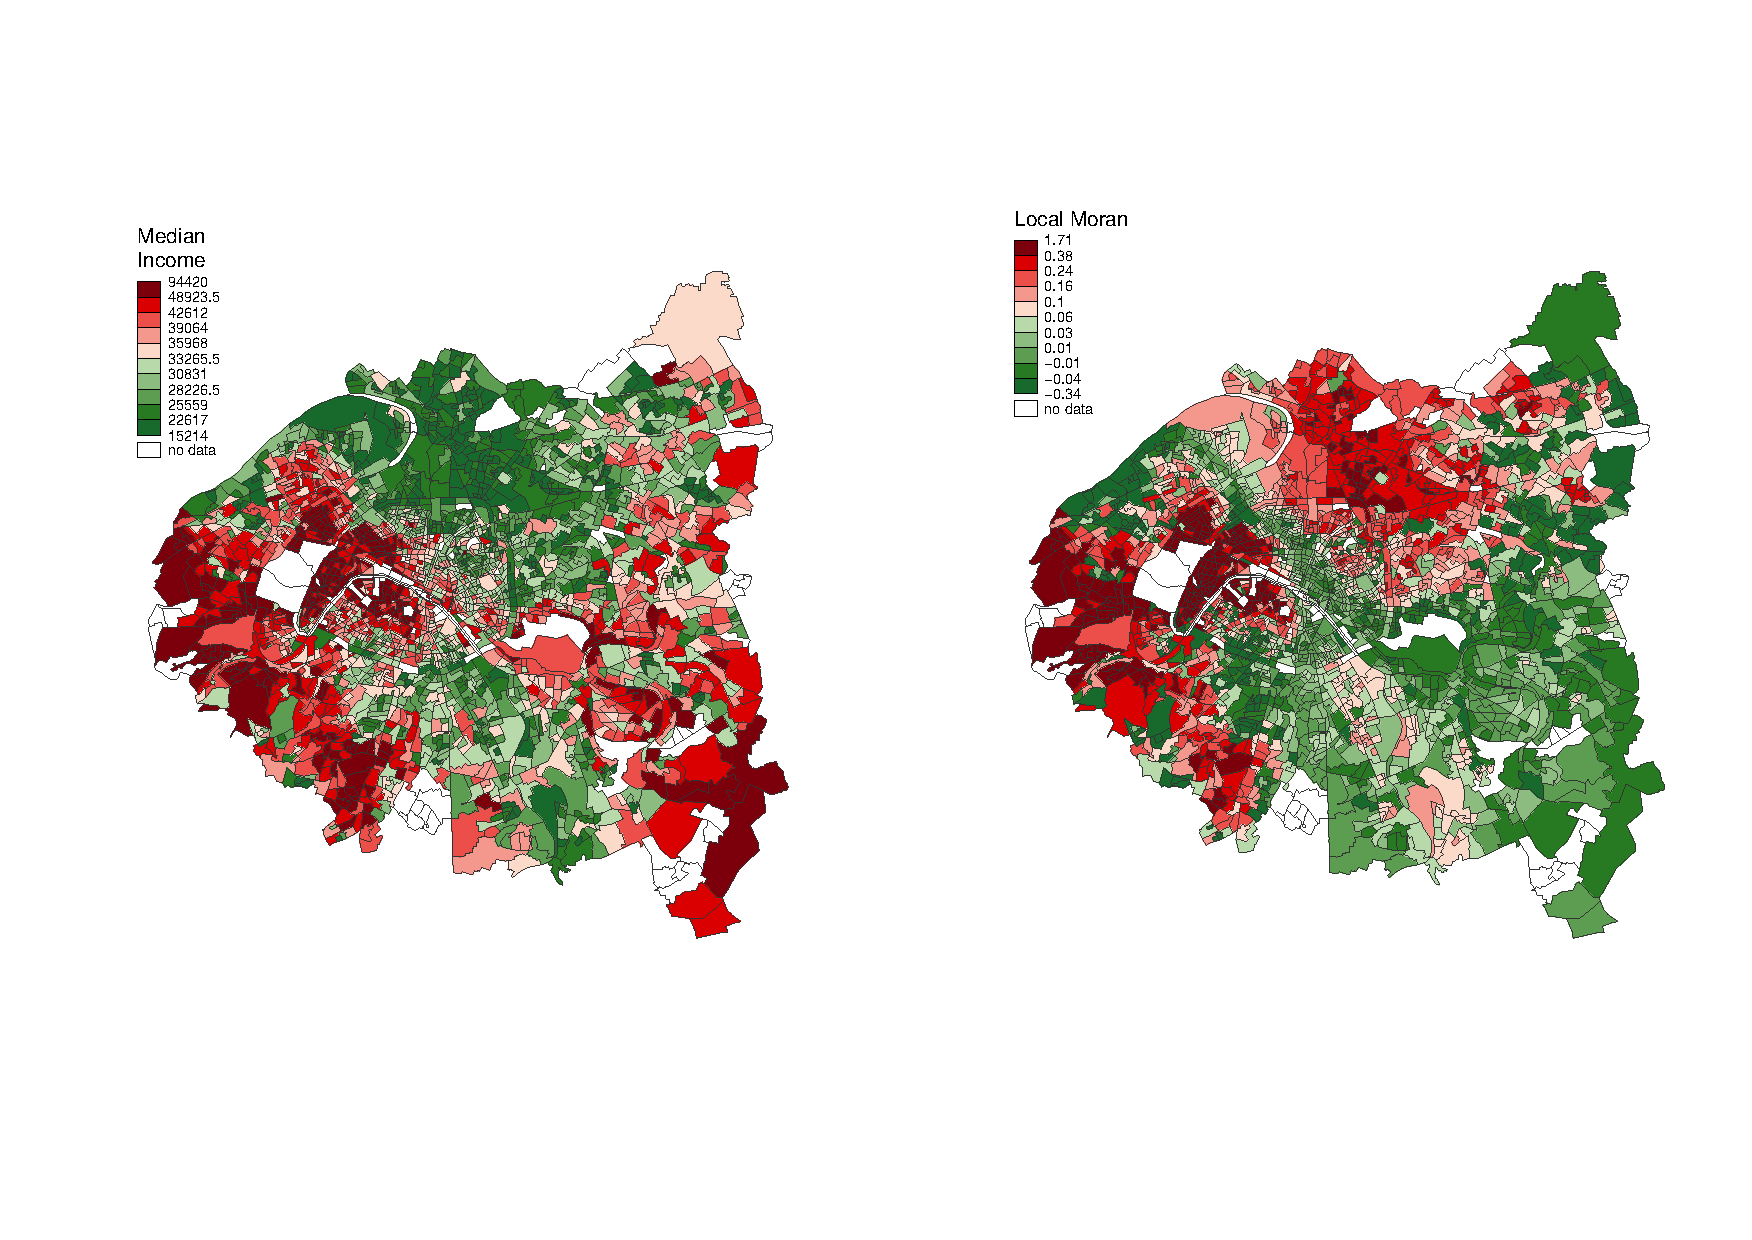
\includegraphics[width=\linewidth]{Figures/RobustnessDiscrepancy/grandParis_income_moran.pdf}
%\caption[Maps of Metropolitan Segregation][Cartes de ségrégation métropolitaine]{\textbf{Maps of Metropolitan Segregation.} Maps show yearly median income on basic statistical units (IRIS) for the three departments constituting mainly the Great Paris metropolitan area, and the corresponding local Moran spatial autocorrelation index, defined for unit $i$ as $\rho_i = N/\sum_{j}w_{ij} \cdot \frac{\sum_{j} w_{ij} (X_j - \bar{X})(X_i - \bar{X})}{\sum_i (X_i - \bar{X})^2}$. The most segregated areas coincide with the richest and the poorest, suggesting an increase of segregation in extreme situations.}{\textbf{Cartes de ségrégation métropolitaine.} Les cartes montrent le revenu annuel médian pour les unités statistiques élémentaires (IRIS) pour les trois départements correspondant globalement à la métropole du Grand Paris, et l'index local d'autocorrelation spatiale de Moran correspondant, défini pour l'unité $i$ par $\rho_i = N/\sum_{j}w_{ij} \cdot \frac{\sum_{j} w_{ij} (X_j - \bar{X})(X_i - \bar{X})}{\sum_i (X_i - \bar{X})^2}$. Les zones les plus ségréguées coincident avec les plus riches et les plus pauvres, suggérant une augmentation de la ségrégation dans les cas extremes.\label{fig:robustness:segreg}}
\caption{}{\label{fig:robustness:segreg}}
\end{figure}
%%%%%%%%%%%%%%%%

\paragraph{Results}{Résultats}


\bpar{
We apply our method with these indicators on the Greater Paris area, constituted of four \emph{d{\'e}partements} that are intermediate administrative units. The recent creation of a new metropolitan governance system~\cite{gilli2009paris} underlines interrogations on its consistence, and in particular on its relation to intermediate spatial inequalities. We show in Fig.~\ref{fig:robustness:segreg} maps of spatial distribution of median income and corresponding local index of autocorrelation. We observe the well-known West-East opposition and district disparities inside Paris as they were formulated in various studies, such as~\cite{guerois2009dynamique} through the analysis of real estate transactions dynamics. We then apply our framework to answer a concrete question that has implications for urban policy : \textit{how are the evaluation of segregation within different territories sensitive to missing data ?} To do so, we proceed to Monte Carlo simulations (75 repetitions) during which a fixed proportion of data is randomly removed, and the corresponding robustness index is evaluated with renormalized indicators. Simulations are done on each \emph{department} separately, each time relatively to the robustness of the evaluation of full Greater Paris. Results are shown in Fig. 2. All areas present a slightly better robustness than the reference, what could be explained by local homogeneity and thus more fiable segregation values. Implications for policy that can be drawn are for example direct comparisons between areas : a loss of 30\% of information on 93 area corresponds to a loss of only 25\% in 92 area. The first being a deprived area, the inequality is increased by this relative lower quality of statistical information. The study of standard deviations suggest further investigations as different response regimes to data removal seem to exist.
}{
La méthode est appliquée avec ces indicateurs à la zone du Grand Paris, constitué de 4 département qui sont des niveaux administratifs intermédiaires. La création récente d'un nouveau système de gouvernance métropolitaine~\cite{gilli2009paris} met en évidence des interrogations sur sa pertinence, notamment sur ses capacités d'atténuer les inégalités spatiales. On peut voir en Fig.~\ref{fig:robustness:segreg} les cartes de la distribution spatiale du revenu médian et de l'index local d'autocorrelation spatiale correspondant. La dichotomie bien connue entre est et ouest est retrouvée ainsi que la disparité des quartiers intra-muros, comme cela été présenté par diverses études, comme~\cite{guerois2009dynamique} à travers l'analyse des dynamiques des transactions immobilières. Notre cadre d'étude est ensuite appliqué à une question concrète ayant des implications pour la prise de décision : \textit{dans quelle mesure une évaluation de la ségrégation au sein de différents territoires est sensible aux données manquantes ?} Pour cela, on procède à des simulations de Monte-Carlo (75 répétitions) pour lesquelles une proportion fixe de données est supprimée aléatoirement, et l'indice de robustesse correspondant est évalué avec les indicateurs normalisés. Les simulations sont faites sur chaque département de façon indépendante, à chaque fois pour une robustesse relative à l'évaluation du Grand Paris complet. Les résultats sont présentés en Fig.~\ref{fig:robustness:sensitivity}. Toutes les zones ont une robustesse légèrement meilleure que la référence, ce qui pourrait être expliqué par une homogénéité locale et donc des indices de ségrégation plus fiables. Les implications pour la prise de décision qui peuvent être par exemple tirées sont des comparaisons directes entre les zones : une perte de 30\% de l'information sur le 93 correspond à une perte de seulement 25\% pour le 92. La première zone étant déjà défavorisée socio-économiquement, l'inégalité est augmentée par cette qualité moindre de l'information statistique. L'étude des déviations standard suggère des études plus approfondies comme différents régimes de réponse à la suppression de données semblent exister.
}



%%%%%%%%%%%%%%%%
\begin{figure}
\centering
%\vspace{-1cm}
%\hspace{-2cm}
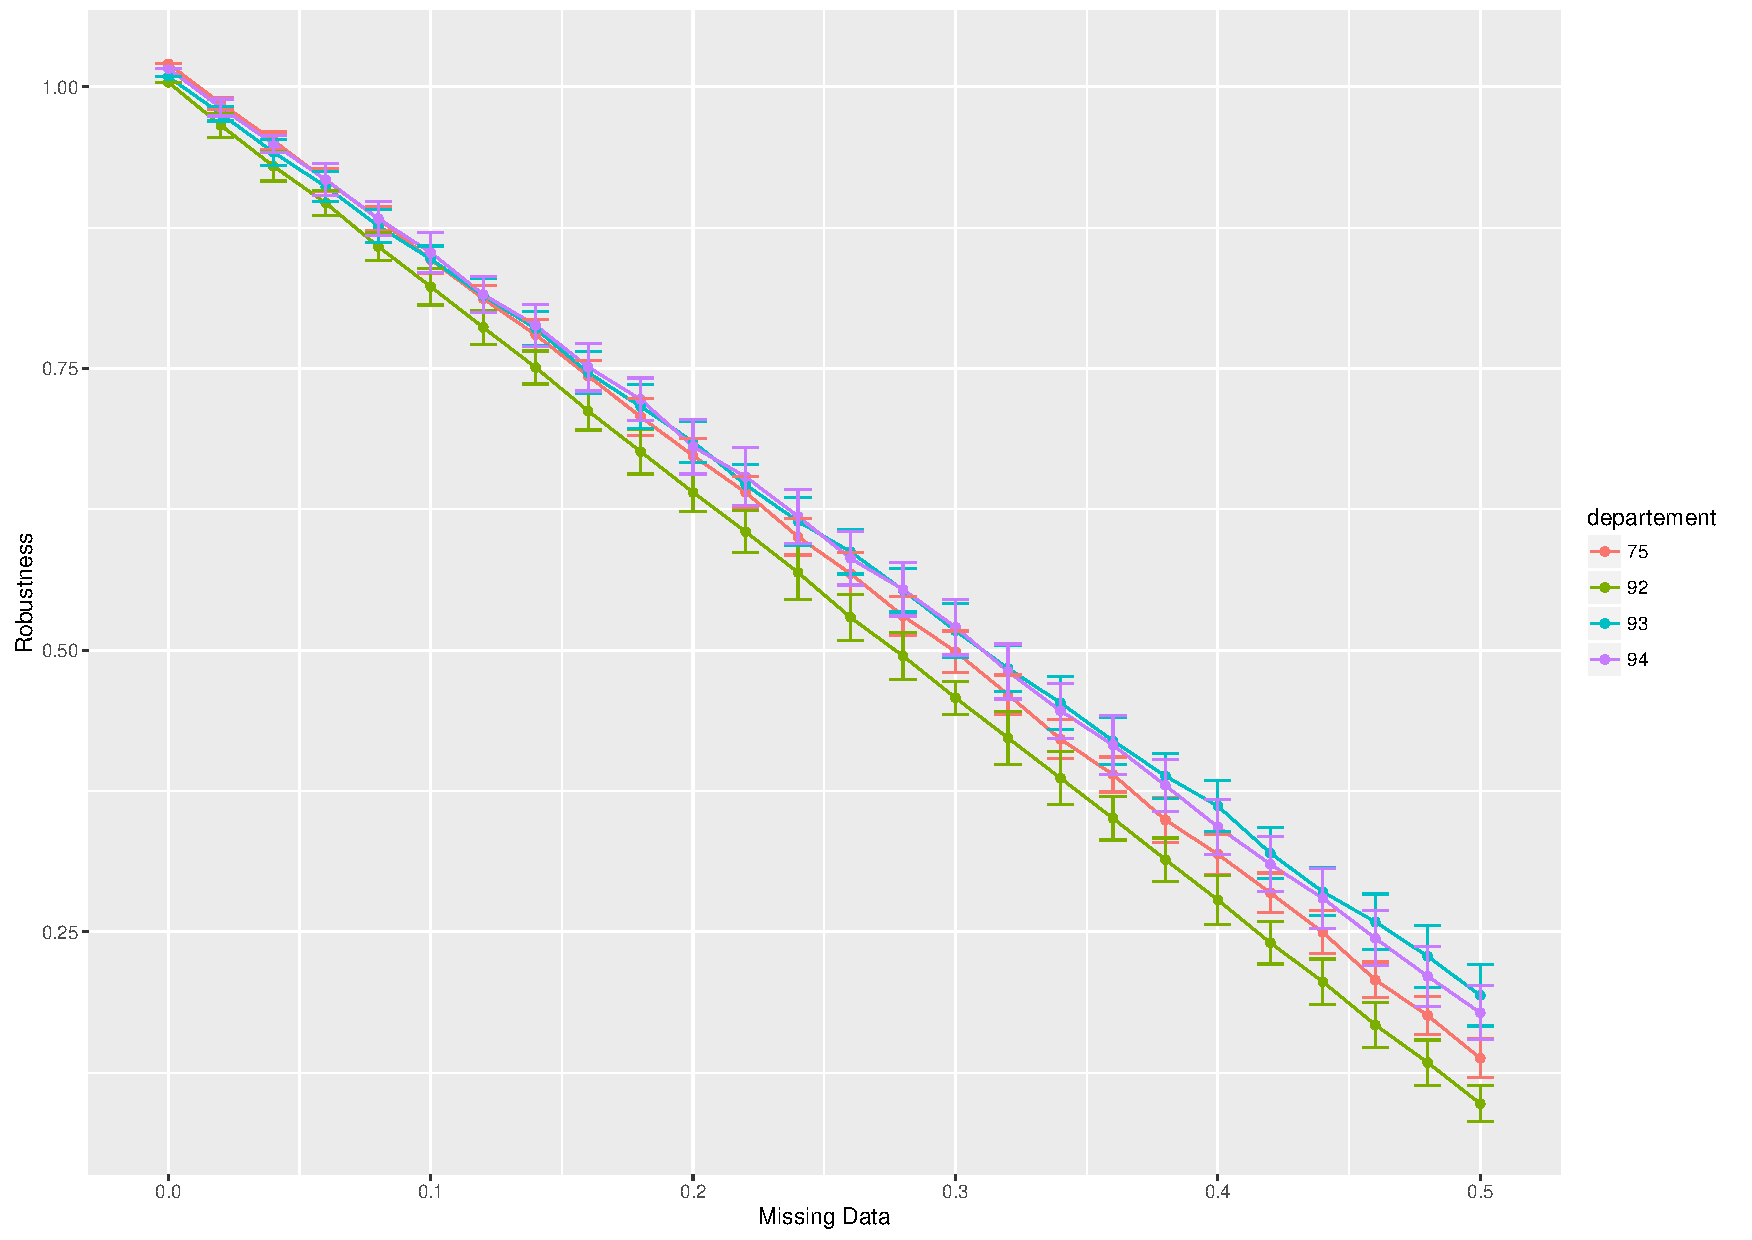
\includegraphics[width=\textwidth]{Figures/RobustnessDiscrepancy/alldeps_rob_renormindics.pdf}
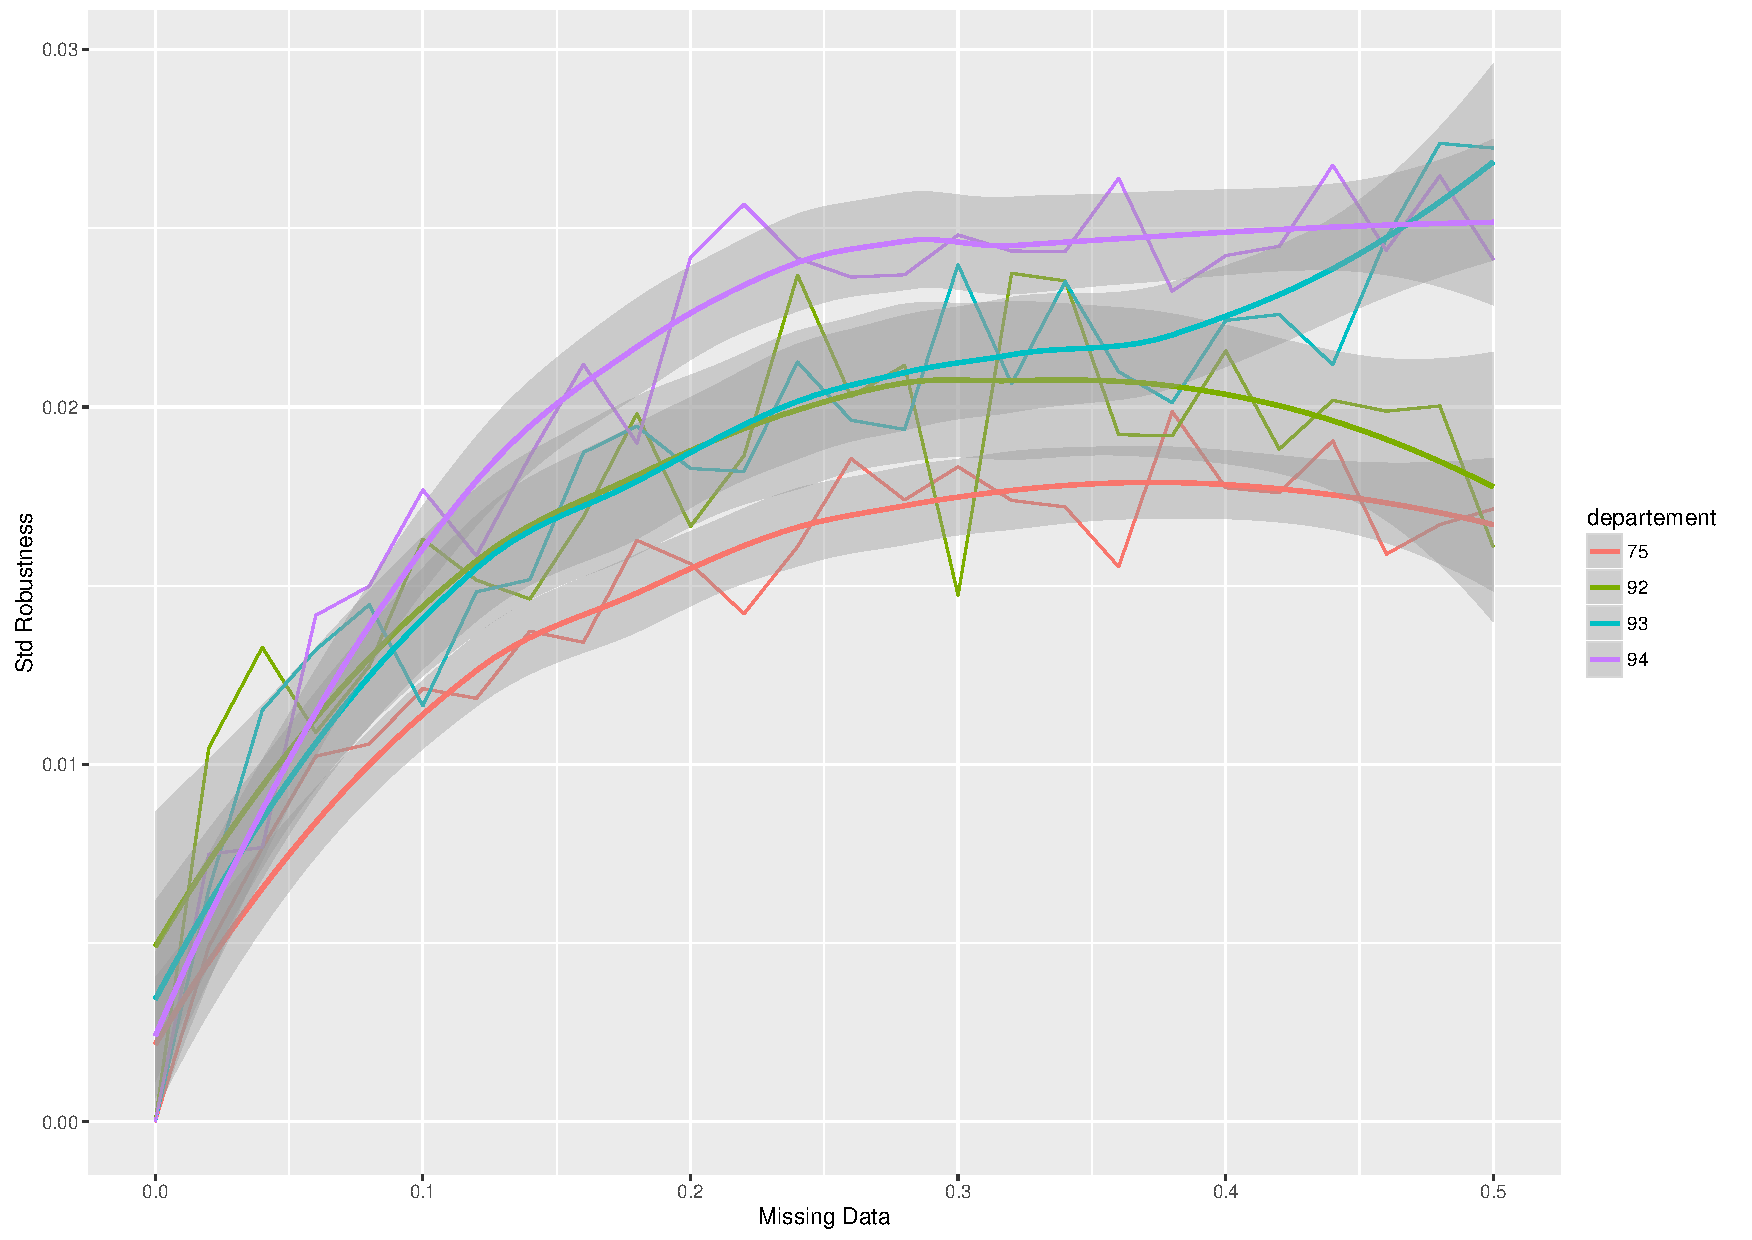
\includegraphics[width=\textwidth]{Figures/RobustnessDiscrepancy/alldeps_robsd_renormindics.pdf}
%\hspace{-2cm}
\caption[Sensitivity of robustness to missing data][Sensibilité de la robustesse aux données manquantes]{\textbf{Sensitivity of robustness to missing data.} \textit{Left.} For each department, Monte Carlo simulations (N=75 repetitions) are used to determine the impact of missing data on robustness of segregation evaluation. Robustness ratios are all computed relatively to full metropolitan area with all available data. Quasi-linear behavior translates an approximative linear decrease of discrepancy as a function of data size. The similar trajectory of poorest departments (93,94) suggest the correction to linear behavior being driven be segregation patterns. \textit{Right.} Corresponding standard deviations of robustness ratios. Different regimes (in particular 93 against others) unveil phase transitions at different levels of missing data, meaning that the evaluation in 94 is from this point of view more sensitive to missing data.}{\textbf{Sensibilité de la robustesse aux données manquantes.} \textit{Gauche.} Pour chaque département, des simulations de Monte-Carlo (N=75 répétitions) sont utilisées pour déterminer l'impact des données manquantes sur la robustesse de l'évaluation de la ségrégation. Les ratios de robustesse sont tous calculés relativement à la région métropolitaine complète avec toutes les données disponibles. Le comportement quasi-linéaire traduit une décroissance approximativement linéaire de la discrépance en fonction de la taille des données. Les trajectoires similaires des départements les plus pauvres (93,94) suggère que la correction au comportement linéaire est fonction des motifs de ségrégation. \textit{Droite.} Déviations standard des ratios de robustesse. Les différents régimes (en particulier le 93 contre les autres) révèlent des transitions de phase à différents niveaux de données manquantes, signifiant que l'évaluation dans le 94 est de ce point de vue plus sensible aux données manquantes.\comment{typo département ?}}
\label{fig:robustness:sensitivity}
\end{figure}
%%%%%%%%%%%%%%%%





%%%%%%%%%%%%%%%%
%% Discussion
%%%%%%%%%%%%%%%%
\subsection{Discussion}{Discussion}


%%%%%%%%%%%%%%%%
\subsubsection{Applicability to Real situations}{Applicabilité à des situations réelles}


\paragraph{Implications for Decision-making}{Implications pour la prise de décision}


\bpar{
The application of our method to concrete decision-making can be thought in different ways. First in the case of a comparative multi-attribute decision process, such as the determination of a transportation corridor, the identification of territories on which the evaluation may be flawed (i.e. has a poor relative robustness) could allow a more refined focus on these and a corresponding revision of datasets or an adapted revision of weights. In any case the overall decision-making process should be made more reliable. A second direction lays in the spirit of the real application we have proposed, i.e. the sensitivity of evaluation to various parameters such as missing data. If a decision appears as reliable because data have few missing points, but the evaluation is very sensitive to it, one will be more careful in the interpretation of results and taking the final decision. Further work and testing will however be needed to understand framework behavior in different contexts and be able to pilot its application in various real situations.
}{
L'application de notre méthode à des situations concrètes de prise de décision peu être pensée de différentes manières. Tout d'abord dans le cas d'un processus multi-attributs à but comparatif, comme la détermination d'un corridor pour une nouvelle infrastructure de transport, l'identification des territoires sur lesquels l'évaluation pourrait être biaisée (i.e. avec une mauvaise robustesse relative) devrait permettre une attention particulière pour ceux-ci, et l'adaptation des jeux de données ou la révision des points en conséquence. Dans tous les cas le processus total devrait être plus fiable. Une autre possibilité ressemble à l'application réelle que nous avons développé, i.e. la sensibilité de l'évaluation à divers paramètres comme les données manquantes. Si une décision parait fiable car la taille de données est grande, mais que l'évaluation est très sensible à la suppression de données, il faudra être prudent pour l'interprétation des résultats et pour la prise de décision finale. Un travail approfondi et de test sera cependant nécessaire pour comprendre le comportement du cadre dans différents contextes et pouvoir piloter son application dans des situations réelles diverses.
}


\paragraph{Integration Within Existing Frameworks}{Intégration au sein de cadres existants}


\bpar{
The applicability of the method on real cases will directly depend on its potential integration within existing framework. Beyond technical difficulties that will surely appear when trying to couple or integrate implementations, more theoretical obstacles could occur, such as fuzzy formulations of functions or data types, consistency issues in databases, etc. Such multi-criteria framework are numerous. Further interesting work would be to attempt integration into an open one, such as e.g. the one described in~\cite{tivadar2014oasis} which calculates various indices of urban segregation, as we have already illustrated the application on metropolitan segregation indexes.
}{
L'applicabilité de la méthode à des cas réels dépendra directement de son intégration potentielle dans des environnements existants. Au delà des difficultés techniques qui apparaissent nécessairement en essayant de coupler ou d'intégrer des implémentations existantes, des obstacles plus théoriques pourraient émerger, comme des formulations floues des fonctions ou des types de données, la cohérence des bases de données, etc. De tels cadres multi-critères sont nombreux. Un développement possible serait l'intégration dans un cadre open-source, comme par exemple celui décrit dans~\cite{tivadar2014oasis} qui calcule divers indices de ségrégation urbaine, comme on l'a déjà illustré pour l'application à la ségrégation métropolitaine.
}

\paragraph{Availability of Raw Data}{Disponibilité des données brutes}


\bpar{
In general, sensitive data such as transportation questionnaires, or very fine granularity census data are not openly available but provided already aggregated at a certain level (for instance French Insee Data are publicly available at basic statistical unit level or larger areas depending on variables and minimal population constraints, more precise data is under restricted access). It means that applying the framework may imply complicated data research procedure, its advantage to be flexible being thus reduced through additional constraints.
}{
De manière générale, des données sensibles comme des questionnaires de transport, ou des données de sondage à granularité très fine, ne sont pas disponibles de manière ouverte, mais fournis de manière déjà agrégée à un certain niveau (comme par exemple les données françaises de l'Insee sont disponibles publiquement au niveau des unités statistiques élémentaires ou pour des zones plus grandes selon les variables et des contraintes de population minimale, les données plus précises étant à accès restreint). Cela signifie que l'application de notre cadre peut impliquer une procédure de recherche de données laborieuse, l'avantage d'être flexible étant alors compensé par ces contraintes additionnelles.
}


%%%%%%%%%%%%%%%%
\subsubsection{Validity of Theoretical Assumptions}{Validité des hypothèses théoriques}


\bpar{
A possible limitation of our approach is the validity of the assumption formulating indicators as spatial integrals. Indeed, many socio-economic indicators are not necessarily depending explicitly on space, and trying to associate them with spatial coordinates may become a slippery slope (e.g. associate individual economic variables with individual residential coordinates will have a sense only if the use of the variable has a relation with space, otherwise it is a non-legitimate artifact). Even indicators which have a spatial value may derive from non-spatial variables, as~\cite{kwan1998space} points out concerning accessibility, when opposing integrated accessibility measures with individual-based non necessarily spatial-based (e.g. individual decisions) measures. Constraining a theoretical representation of a system to fit a framework by changing some of its ontological properties (always in the sense of real meaning of objects) can be understood as a violation of a fundamental rule of modeling and simulation in social science given in~\cite{banos2013HDR}, that is that there can be an universal ``language'' for modeling and some can not express some systems, having for consequence misleading conclusion due to ontology breaking in the case of an over-constrained formulation.
}{
Une limitation possible de notre approche est la validité de l'hypothèse qui formule les indicateurs comme des intégrales spatiales. En fait, de nombreux indicateurs socio-économiques ne dépendent pas nécessairement directement de l'espace, et essayer de les associer à des coordonnées peut entraîner sur une pente glissante (par exemple, associer des variables économiques individuelles à des coordonnées résidentielles aura un sens seulement si la variable à une relation à l'espace, autrement un devient un artefact superflu). Même des indicateurs qui ont une valeur spatiale peuvent dériver de variables non-spatiales, comme~ \cite{kwan1998space} le souligne au sujet de l'accessibilité, en opposant les mesures d'accessibilité intégrée aux mesures individu-centrées mais pas forcément basée sur l'espace (comme par exemple des décisions individuelles). Contraindre une représentation théorique d'un système pour le faire rentrer dans un cadre en changeant certaines de ses propriétés ontologiques (toujours dans le sens de la signification réelle des objets) peut être compris comme une violation d'une des règles pour la modélisation et la simulation en sciences sociales données par~\cite{banos2013HDR}, car cela impliquerait qu'il pourrait exister un langage universel pour la modélisation, malgré qu'il ne puisse retranscrire certains systèmes, ayant pour conséquences des conclusions errantes à cause d'une rupture d'ontologie dans le cas d'une formulation sur-contrainte.
}

%%%%%%%%%%%%%%%%
\subsubsection{Framework Generality}{Généralité du Cadre}


\bpar{
We argue that the fundamental advantage of the proposed framework is its generality and flexibility, since robustness of the evaluations are obtained only through data structure if ones relaxes constraints on the value of weight. Further work should go towards a more general formulation, suppressing for example the linear aggregation assumption. Non-linear aggregation functions would require however to present particular properties regarding integral inequalities. For example, similar results could search in the direction of integral inequalities for Lipschitzian functions such as the one-dimensional results of~\cite{dragomir1999ostrowski}.
}{
Nous soutenons qu'un des avantages fondamentaux de notre cadre est sa généralité et sa flexibilité, puisque la robustesse des évaluations est obtenue seulement par la structure des données si l'on relaxe les hypothèses sur les valeurs des poids. Des approfondissement pourraient inclure une formulation plus générale, en supprimant par exemple l'hypothèse d'agrégation linéaire. Des fonctions d'agrégation non-linéaires demanderaient toutefois de vérifier certaines propriétés regardant les inégalités intégrales. Par exemple, des résultats similaires pourraient être obtenus en s'orientant vers des inégalités intégrales pour fonctions Lipschitziennes, comme les résultats en une dimension de~\cite{dragomir1999ostrowski}.
}


%%%%%%%%%%%%%%%%
%% Conclusion
%%%%%%%%%%%%%%%%
\subsection*{Conclusion}{Conclusion}


\bpar{
We have proposed a model-independent framework to compare the robustness of multi-attribute evaluations between different urban systems. Based on data discrepancy, it provide a general definition of relative robustness without any assumption on model for the system, but with limiting assumptions that are the need of linear aggregation and of indicators being expressed through spatial kernel integrals. We propose a toy implementation based on real data for the city of Paris, numerical results confirming general expected behavior, and an implementation on real data for income segregation on Greater Paris metropolitan areas, giving possible insights into concrete policy questions. Further work should be oriented towards sensitivity analysis of the method, application to other real cases and theoretical assumptions relaxation, i.e. the relaxation of linear aggregation and spatial integration.
}{
Nous avons proposé un cadre indépendant du modèle pour comparer la robustesse d'évaluations multi-attributs entre différents systèmes urbains. A partir de la discrépance des données, on fournit une définition générale de la robustesse relative sans aucune hypothèse de modèle pour le système, mais en supposant une agrégation linéaire des objectifs et des indicateurs exprimés comme des intégrales à noyaux. Nous proposons une première implémentation preuve de concept pour la ville de Paris pour laquelle les résultats numériques confirment la tendance générale attendue, et une implémentation sur des données réelles pour la ségrégation de revenus pour la région métropolitaine du Grand Paris, fournissant des réponses possibles à des questions de prise de décision plus concrètes. Des développements possibles peuvent inclure une analyse de sensibilité de la méthode, des applications à d'autres cas réels et une relaxation des hypothèses théoriques, c'est à dire de l'agrégation linéaire et de l'intégration spatiale.\comment{confusion spatial/ kernel ? -> idem à l'oral ?}
}


%\section*{Acknowledgments}

%The author would like to thank Julien Keutchayan (Ecole Polytechnique de Montr{\'e}al) for suggesting the original idea of using discrepancy, and anonymous reviewers for the useful comments and insights.









% quant epistemo after as a transition to more quanti part ?

%%%%%%%%%%%%%%%%%%%%%%%%%%%%%
% Chapter : Quantitative Epistemology


\newpage

%----------------------------------------------------------------------------------------

\section{An epistemological Approach}{Une Approche Epistémologique}

\label{sec:quantepistemo}


%----------------------------------------------------------------------------------------


\bpar{
A corollary of the thematic background introduced in chapter~\ref{ch:thematic} is the need of an understanding of involved disciplines themselves to be able to build integrated heterogeneous models. The potentialities of couplings and integrations are greatly determined by existing approaches and corresponding gaps. This implies an advanced epistemological study in each field, that we propose to tackle in a systematic and quantitative way. This deliberate choice may shadow elaborated epistemological considerations but fits our purpose of preliminary investigations for the construction of models, as it may reveal investigation directions.
}{
Un corolaire de la matière thématique introduite\comment[FL]{phrase a reprendre} en chapitre~\ref{ch:thematic} est le besoin d'une compréhension des disciplines impliquées elles-même pour être en mesure de construire des modèles hétérogènes intégrés. Les possibilités de couplage et d'intégration\comment[FL]{definir, differencier, clarifier}[(JR) cf intro] sont hautement déterminées par les approches existantes et les lacunes correspondantes qui ont été exposées dans la section précédente~\ref{sec:modelingsa}. Cela implique une étude épistémologique avancée dans chaque champ, que nous proposons de mener de manière quantitative et systématique. Ce choix délibéré\comment[FL]{choix qui n'est pas justifie de facon satisfaisante. pourquoi = pourquoi faire ? quattends tu de cela et pourquoi l'approche classique ne convient pas ?}[(JR) importance de la reflexivite et de l'epistmo quanti pour les approches integratives] pourrait occulter des considérations épistémologiques élaborées mais suit notre objectif d'investigations préliminaires pour la construction de modèles, en révélant potentiellement des directions de recherche.
}


\bpar{
We describe and explore first a systematic review exploration algorithm, that retrieve corpuses of references through iterative semantic extraction. We describe then briefly possible extended bibliometrics by presenting an external example of application. We finally suggest possible development directions towards unsupervised data and text-mining.
}{
Nous décrivons et explorons d'abord un algorithme de revue systématique algorithmique, qui reconstruit des corpus de références par une extraction sémantique itérative\comment[FL]{ajouter precisions}. Nous procédons ensuite à une analyse de réseaux, couplant réseau de citation et réseau sémantique, pour préciser les contours des disciplines impliquées. Nous suggérons finalement des possibles extensions vers de l'apprentissage non-supervisé et la fouille de texte complets pour une extraction automatique de la structure de modèles par exemple.
}





%----------------------------------------------------------------------------------------



\subsection{Algorithmic Systematic Review}{Revue Systématique Algorithmique}


\bpar{
A broad bibliographical study suggests a scarcity of quantitative models of simulation integrating both network and urban growth. This absence may be due to diverging interests of concerned disciplines, resulting in a lack of communication.  We propose to proceed to an algorithmic systematic review to give quantitative elements of answer to this question. A formal iterative algorithm to retrieve corpuses of references from initial keywords, based on text-mining, is developed and implemented. We study its convergence properties and do a sensitivity analysis. We then apply it on queries representative of the specific question, for which results tend to confirm the assumption of disciplines compartmentalization.
}{
Une étude bibliographique étendue suggère une rareté\comment[FL]{par rapport a quoi ?} des modèles quantitatifs de simulation qui intègrent à la fois la croissance urbaine et la croissance des réseaux. Cette absence pourrait être due aux intérêts divergents des acteurs des disciplines\comment[FL]{peut on parler d'interets de disciplines de facon univoque ?}[(JR) acteurs des disciplines ?] concernées qui induiraient un manque de communication. Nous proposons de procéder à une revue de la littérature systématique et algorithmique pour donner des éléments de réponse quantitatifs à cette question. Un algorithme itératif formel pour construire des corpus de références à partir de mots-clés initiaux, basé sur l'analyse textuelle, est développé et mis en oeuvre. Nous étudions ses propriétés de convergence et procédons à une analyse de sensibilité. Nous l'appliquons ensuite à des requêtes représentatives de notre question spécifique, pour lesquelles les résultats tendent à confirmer l'hypothèse d'isolation relative des disciplines.
}



\subsubsection{In search of models of co-evolution}{En recherche de modèles de co-évolution}


\bpar{
Transportation networks and urban land-use are known to be strongly coupled components of urban systems at different scales~\cite{bretagnolle2009organization}. One common approach is to consider them as co-evolving, avoiding misleading interpretations such as the myth of structural effect of transportation infrastructures~\cite{offner1993effets}. A question rapidly arising is the existence of models endogeneizing this co-evolution, i.e. taking into account simultaneous urban and network growth. We try to answer it using an algorithmic systematic review. We propose in this section, after a brief state of the art of existing literature, to present such an approach by formalizing the algorithm, which results are then presented and discussed. 
}{
Comme développé en~\ref{sec:networkterritories}, les réseaux de transport et l'usage du sol urbain sont connus pour être des composantes au couplage complexe au sein des systèmes urbains\comment[FL]{trop rapide, cest une lectire possible mais pas une realite bien connue}, à différentes échelles~\cite{bretagnolle2009organization}. Une approche commune est de les considérer comme étant en co-évolution, tout en évitant les interprétations trompeuses\comment[FL]{la aussi tu simplifies trop} comme le mythe des effets structurants des infrastructures de transport~\cite{offner1993effets}. Une question qui se présente rapidement\comment[FL]{mal dit} est l'existence de modèles endogénéisant cette co-évolution, i.e. prenant en compte simultanément la croissance urbaine et celle du réseau. Nous essayons d'y répondre par une revue systématique algorithmique\comment[FL]{1) tu l'as deja dit, 2) tu ne justifies pas cette approche}. Nous proposons dans cette section de développer cette approche en formalisant l'algorithme, dont les résultats sont ensuite présentés et discutés.
}


\subsubsection{Modeling Interactions between Urban Growth and Network Growth}{Modéliser les interactions entre croissance urbaine et croissance des réseaux}

Nous avons revu selon divers point de vue les efforts de modélisation des interactions entre territoires et réseaux dans la section précédente~\ref{sec:modelingsa}. Cet état de l'art nous suggère fortement des domaines relativement cloisonnés et s'intéressant à des problématiques différentes.



\subsubsection{Bibliometric Analysis}{Analyse Bibliométrique}


\bpar{
Literature review is a crucial preliminary step for any scientific work and its quality and extent may have a dramatic impact on research quality. Systematic review techniques have been developed, from qualitative review to quantitative meta-analyses allowing to produce new results by combining existing studies \cite{rucker2012network}. Ignoring some references can even be considered as a scientific mistake in the context of emerging information systems~\cite{lissacksubliminal}. We aim to take advantage of such techniques to tackle our issue.
Indeed, observing the form of the bibliography obtained in previous section raises some hypothesis. It is clear that all components are present for co-evolutive models to exist but different concerns and objectives seem to stop it. As it was shown by \cite{commenges:tel-00923682} for the concept of mobility, for which a ``small world of actors'' relatively closed invented a notion ad hoc, using models without accurate knowledge of a more general scientific context, we could be in an analog case for the type of models we are interested in. Restricted interactions between scientific fields working on the same objects but with different purposes, backgrounds and at different scales, could be at the origin of the relative absence of co-evolving models. 
While most of studies in bibliometrics rely on citation networks \cite{2013arXiv1310.8220N} or co-autorship networks \cite{2014arXiv1402.7268S}, we propose to use a less explored paradigm based on text-mining introduced in~\cite{chavalarias2013phylomemetic}, that obtain a dynamic mapping of scientific disciplines based on their semantic content. For our question, it has a particular interest, as we want to understand content structure of researches on the subject. We propose to apply an algorithmic method described in the following. The algorithm proceeds by iterations to obtain a stabilized corpus from initial keywords, reconstructing scientific semantic landscape around a particular subject.
}{
Avec l'avènement des nouveaux moyens techniques et des nouvelles sources de données, la revue de littérature classique tend à se coupler à des revues automatiques. Des techniques de revue systématique ont été développées, des revues qualitatives aux meta-analyses quantitatives qui permettent de produire des nouveaux résultats par combinaison d'études existantes~\cite{rucker2012network}. Passer sous silence certaines références peut même être considéré comme une erreur scientifique dans le contexte de l'émergence des systèmes d'information qui par l'accès plus aisé à l'information rend difficilement justifiable l'omission de références clés~\cite{lissacksubliminal}.\comment[FL]{phrase risquee : est-tu certain de n'etre passe a cote de rien ? par exemple as tu lu Brotchie 1984 ?}[(JR) justement la est la contradiction et la justification de l'approche : maximiser couverture, tout en sachant qu'on ne peut pas tout couvrir (perspectivisme) - a developper] Nous proposons de tirer parti de telles techniques pour traiter notre problème.
En effet, l'observation de la bibliographie obtenue dans la section précédente soulève une hypothèse. On peut postuler sans risques\comment[FL]{tournure a reprendre} à partir de la revue précédente~\ref{sec:modelingsa} Il semble clair que toutes les briques sont présentes pour l'existence de modèles co-évolutifs mais des questionnements et objectifs différents semblent la stopper. Comme montré par~\cite{commenges:tel-00923682} pour le concept de mobilité, pour lequel un ``petit monde d'acteurs''\comment[FL]{sens ?} relativement fermé, en l'occurence les Corpsards de l'Ecole des Ponts et Chaussées\comment[FL]{tu generalises trop}, a inventé une notion \emph{ad hoc}, utilisant des modèles sans connaissance préalable d'un contexte scientifique plus général. On pourrait se trouver dans un cas similaire pour le type de modèles auxquels on s'intéresse. Des interactions restreintes entre des champs scientifiques travaillant sur les mêmes objets mais avec des objectifs et contextes divergents, et à des échelles différentes, pourrait être à l'origine de l'absence de modèles co-évolutifs. Tandis que la majorité des études en bibliométrie se reposent sur les réseaux de citation~\cite{2013arXiv1310.8220N} ou les réseaux de co-auteurs~\cite{2014arXiv1402.7268S}, nous proposons d'utiliser un paradigme moins exploré, basé sur l'analyse textuelle, introduit par~\cite{chavalarias2013phylomemetic}, qui obtient une cartographie dynamique des disciplines scientifiques en se basant sur leur contenu sémantique. Nous postulons que cette couche supplémentaire d'information apporte une information complémentaire\comment[FL]{c'est une posture originale, dommage de ne pas avoir applique de methode plus classique pour commencer}[(JR) c'est l'objet du 2.1], nécessaire pour appréhender la diversité des domaines. La méthode est particulièrement adaptée pour notre étude puisque nous voulons comprendre la structure du contenu des recherches sur le sujet. Nous appliquons une approche algorithmique décrite par la suite. L'algorithme procède par itérations pour obtenir un corpus stabilisé à partir de mots-clés initiaux, reconstruisant l'horizon sémantique scientifique autour d'un sujet donné.
}


\paragraph{Description of the Algorithm}{Description de l'Algorithme}


\bpar{
Let $A$ be an alphabet, $A^{\ast}$ corresponding words and $T = \cup_{k\in \mathbb{N}} {A^{\ast}}^k$ texts of finite length on it. A reference is for the algorithm a record with text fields representing title, abstract and keywords. Set of references at iteration $n$ will be denoted $\mathcal{C} \subset T^3$. We assume the existence of a set of keywords $\mathcal{K}_n$, initial keywords being $\mathcal{K}_0$. An iteration goes as follows :

\begin{enumerate}
\item A raw intermediate corpus $\mathcal{R}_n$ is obtained through a catalog request providing previous keywords $\mathcal{K}_{n-1}$.
\item Overall corpus is actualized by $\mathcal{C}_n = \mathcal{C}_{n-1} \cup \mathcal{R}_n$.
\item New keywords $\mathcal{K}_n$ are extracted from corpus through Natural Language Processing treatment, given a parameter $N_k$ fixing the number of keywords.
\end{enumerate}

The algorithm stops when corpus size becomes stable or a user-defined maximal number of iterations has been reached. Fig.~\ref{fig:quantepistemo:algo} shows the global workflow.
}{
Soit $A$ un alphabet (un ensemble arbitraire de symboles), $A^{\ast}$ les mots correspondants\comment[FL]{sens ?} et $T = \cup_{k\in \mathbb{N}} {A^{\ast}}^k$\comment[FL]{que signifie cette notation ?}[(JR) INF101] les textes de longueur finie sur celui-ci. Ce qu'on nomme une référence est pour l'algorithme un enregistrement avec des champs textuels représentant le titre, le résumé et les mots-clés. L'ensemble de références\comment[FL]{on ne voit pas le lien avec Astar} à l'itération $n$ sera noté $\mathcal{C} \subset T^3$\comment[FL]{pourquoi ny a til pas n ?}[(JR) on parle d'un element] : il s'agit d'un sous-ensemble de triplets de textes. Nous supposons l'existence d'un ensemble de mots-clés $\mathcal{K}_n$, les mots-clés initiaux étant $\mathcal{K}_0$, spécifiés par l'utilisateur\footnote{On pourrait également partir d'un corpus $\mathcal{C}_0$, mais il s'agit plutôt de l'esprit de la méthodologie présentée dans la sous-section suivante. Nous nous en tiendrons ici pour cette exploration préliminaire en assumant le caractère arbitraire forcément biaisé de cette spécification.\comment[FL]{oui mais justement l'explication du choix de ce corpus est cruciale}}. Une itération procède de la manière suivante :

\comment[FL]{Commencer par expliquer les objets qui seront utilises}

\begin{enumerate}
\item Un corpus intermédiaire brut $\mathcal{R}_n$ est obtenu par une requête à un catalogue\footnote{La dépendance au catalogue devant sûrement introduire un biais que nous ne pouvons contrôler, une analyse de sensibilité ou le croisement de divers catalogues étant hors de propos pour cette analyse exploratoire.}
 auquel on fourni les mots-clés précédents $\mathcal{K}_{n-1}$.
\item Le corpus total est actualisé par $\mathcal{C}_n = \mathcal{C}_{n-1} \cup \mathcal{R}_n$.
\item Les nouveaux mot-clés $\mathcal{K}_n$ sont extraits du corpus par Traitement du Language Naturel (NLP), étant donné un paramètre fixé $N_k$\comment[FL]{pourquoi cette notation ?} donnant le nombre de mot-clés.\comment[FL]{expliquer ce dont il s'agit}
\end{enumerate}

L'algorithme termine quand la taille du corpus devient stable\comment[FL]{quel sens? quel critere ?} ou quand un nombre maximal d'itérations défini par l'utilisateur est atteint. La figure~\ref{fig:quantepistemo:algo} synthétise le processus général.
}


%%%%%%%%%%%%%%%%%%%%%%%%%%%%
\begin{figure}
\centering
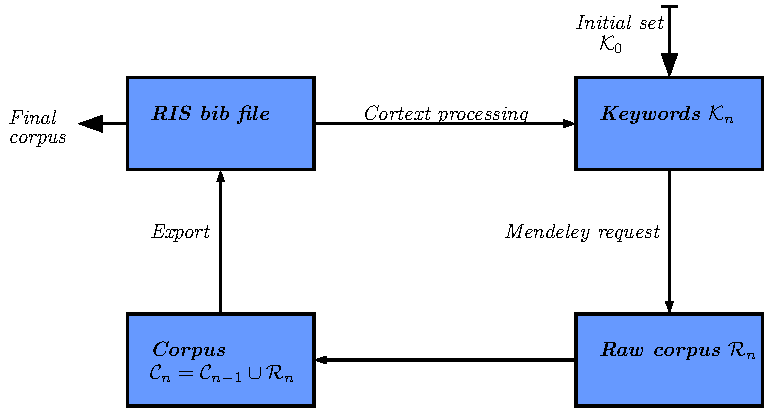
\includegraphics[width=0.8\linewidth]{Figures/QuantEpistemo/schema_algo}
\caption[Systematic review algorithm workflow][Algorithme de revue systématique]{Global workflow of the algorithm, including implementation details: catalog request is done through Mendeley API; final state of corpuses are RIS files.\label{fig:quantepistemo:algo}}{Architecture globale de l'algorithme, incluant des détails d'implémentation : la requête au catalogue est faite via l'API Mendeley \comment[FL]{tu ne l'as pas dit auparavant}; les corpus finaux sont sous forme de fichiers RIS.\label{fig:quantepistemo:algo}\comment[FL]{traduire ; pourquoi mendeley ?}}
\end{figure}
%%%%%%%%%%%%%%%%%%%%%%%%%%%%



%%%%%%%%%%%%%%%%%%%%%%%%%%%%
\paragraph{Results}{Résultats}



\bpar{
Once the algorithm is partially validated, we apply it to our question. We start from five different initial requests that were manually extracted from the various domains identified in the bibliography (that are ``city system network'', ``land use transport interaction'', ``network urban modeling'', ``population density transport'', ``transportation network urban growth''). We take the weakest assumption on parameter $N_k=100$, as it should less constrain reached domains. After having constructed corpuses, we study their lexical distances as an indicator to answer our initial question. Large distances would go in the direction of the assumption made above, i.e. that discipline self-centering may be at the origin of the lack of interest for co-evolutive models. We show in Table~\ref{tab:quantepistemo:lexical} values of relative lexical proximity, that appear to be significantly low, confirming this assumption.
}{
Les détails précis concernant l'implémentation de l'algorithme ainsi qu'une analyse de sensibilité pour vérifier la convergence sur un échantillon de requêtes initiales (typiques des champs étudiés\comment[FL]{?}) sont donnés en Appendice~\ref{app:sec:quantepistemo}. Lorsque l'algorithme a été partiellement validé par cette analyse, nous l'appliquons à notre question. Nous partons de cinq différentes requêtes initiales qui ont été manuellement extraites des divers domaines identifiés dans la bibliographie (qui sont ``city system network'', ``land use transport interaction'', ``network urban modeling'', ``population density transport'', ``transportation network urban growth'')\comment[FL]{ces mots sont nombreux, quel impact sur l'algo ?}\comment[FL]{du coup tu exclues totalement la literature francophone. pourquoi ce choix ?}\footnote{Ce choix est arbitraire,\comment[FL]{on espere que non} cette étude étant préliminaire on admet de travailler potentiellement sur des échantillons. Par exemple, l'utilisation de ``co-evolution'' n'est pas concluante car trop peu d'articles utilisent cette formulation.}. Nous prenons l'hypothèse la plus faible pour le paramètre $N_k=100$ (plus $N_k$ est grand, plus les domaines atteints devraient être moins restreints et donc plus des résultats de distance seront significatifs)\label{tab:quantepistemo:lexical}\comment[FL]{phrase non comprehensible}. Après avoir construit les corpus, nous étudions leur cohérence lexicale comme un indicateur de réponse à notre question initiale. De grande distances devraient confirmer l'hypothèse formulée ci-dessus, i.e. que des disciplines auto-centrées pourraient être à l'origine d'un manque d'intérêt pour des modèles co-évolutifs. La table~\ref{tab:quantepistemo:lexical} montre les valeurs\comment[FL]{tu n'as pas explique comment tu quantifies cela} de la proximité lexicale relative, qui est significativement basse\comment[FL]{sens ?} sachant que les chiffres peuvent directement s'interpréter comme une proportion de mots en co-occurrence, ce qui tend à confirmer notre hypothèse. Pour être plus précis tout de même, il faudrait un modèle nul\comment[FL]{?} avec des corpus aléatoires par exemple, ce qui pourrait faire l'objet de développements futurs. 
}




%%%%%%%%%%%%%%%%%%%%%%%%%%%%
\begin{table}
\caption[Stationary lexical proximities][Proximités lexicales stationnaires]{Symmetric matrix of lexical proximities between final corpuses, defined as the sum of overall final keywords co-occurrences between corpuses, normalized by number of final keywords (100). We obtain very low values, confirming that corpuses are significantly far. Size of final corpuses is given as $W$.\label{tab:quantepistemo:lexical}}{Matrice symétrique des proximités lexicales entre les corpus finaux, définies comme la somme des co-occurrences totale de mots-clés finaux entre corpus, normalisé par le nombre de mots-clés finaux (100). La taille des corpus finaux est donnée par $W$. Les valeurs obtenues pour les proximités sont considérablement faibles, ce qui confirme que les corpus sont éloignés de manière significative (voir texte).\comment[FL]{ce tableau est difficilement comprehensible ; traduire ; trop de chiffres significatifs.}\label{tab:quantepistemo:lexical}}
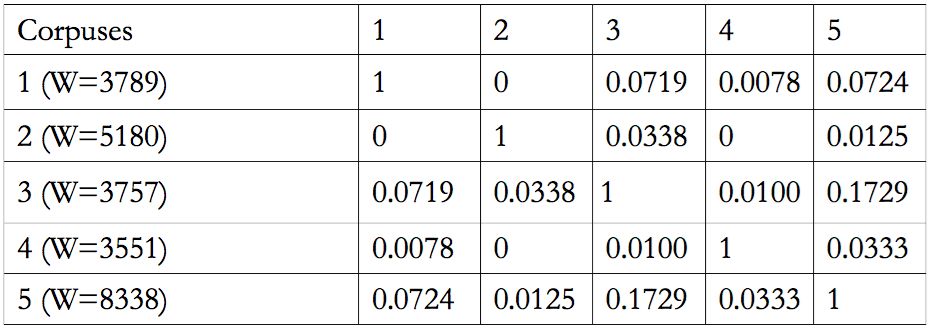
\includegraphics[width=0.8\linewidth]{Figures/QuantEpistemo/corpusesDistances}
\end{table}
%%%%%%%%%%%%%%%%%%%%%%%%%%%%




\bpar{
Possible developments can include the construction of citation networks through an automatic access to Google Scholar that provides backward citations. The confrontation of inter-cluster coefficients on the citation network for the different corpuses with lexical consistence are an essential aspect of a further validation of our results.
}{
Les développements possibles incluent la construction de réseaux de citation via un accès automatique à Google Scholar\comment[FL]{pourquoi cette plateforme et pas une autre ?} qui fournit les citations entrantes. La confrontation des coefficients inter-clusters pour le réseau de citations entre les différents corpus avec la cohérence lexicale est un aspect clé d'une validation approfondie des résultats.
}



\bpar{
The disturbing absence of models simulating the co-evolution of transportation networks and urban land-use, confirmed through a state-of-the-art covering many domain, may be due to the absence of communication between scientific disciplines studying different aspects of that problems. We have proposed an algorithmic method to give elements of answers through text-mining-based corpus extraction. First numerical results seem to confirm the assumption. However, such a quantitative analysis should not be considered alone, but rather come as a back-up for qualitative studies that will be the object of further work, such as the one lead in~\cite{commenges:tel-00923682}, in which questionnaires with historical actors of modeling provide highly relevant information.
}{
L'absence peu explicable\comment[FL]{pourquoi cette hypothese ?} a priori de modèles qui simulent la co-évolution des réseaux de transport et de l'usage du sol urbain, qui se confirme à première vue par un état de l'art couvrant des domaines disparates, pourrait être due à l'absence de communication entre les disciplines scientifiques étudiant différents aspects du problème. D'autres explications possibles qui en sont proches peuvent par exemple être le manque de cas d'application concrets de tels modèles vu les échelles temporelles mises en jeu et donc l'absence de financement propre - ce qui n'est pas si loin de l'absence d'une discipline y consacrant certains de ses objets. Cette question des portées et des échelles des modèles fera l'objet de la meta-analyse à la section suivante~\ref{sec:modelography}. Ainsi, nous ici avons proposé une méthode algorithmique pour donner des éléments de réponse par l'extraction de corpus basée sur l'analyse textuelle. Les premiers résultats numériques semblent confirmer l'hypothèse. Cependant, une telle analyse quantitative ne doit pas être considérée seule, mais devrait plutôt venir comme soutien à des études qualitatives qui peuvent être l'objet de développements futurs, comme celle menée dans~\cite{commenges:tel-00923682}, dans laquelle des questionnaires avec des acteurs historiques fournit des informations extrêmement pertinentes. \comment[FL]{ET A UNE REVUE DE BIBLIO CLASSIQUE}[(JR) faite en 2.1]
}




%--------------------------------------------------------------


%%%%%%%%%%%%%%%%%%%%%%%%
%\subsection[Indirect Bibliometrics][Bibliométrie indirecte]{Indirect bibliometrics through Complex Network analysis}{Bibliométrie Indirecte par Analyse de Réseaux Complexes}
\subsection{Indirect Bibliometrics}{Bibliométrie indirecte}

\label{subsec:indirectbibliometrics}


\bpar{
As described before, semantic analysis of final corpus does not contain all the information on disciplinary compartmentation nor on patterns of propagation of scientific knowledge as the ones contained in citation networks for example. Furthermore, data collection in the previous algorithm is subject to convergence towards self-consistent themes because of the proper structure of the method. It may give more insight about scientific social patterns of ontological choices in modeling to study communities in broader networks, that would more correspond to disciplines (or sub-disciplines depending on granularity level). We propose to reconstruct disciplines around our thematic, to obtain a more precise view of interdisciplinarity and the scientific landscape on our subject.
}{
Comme décrit précédemment, l'analyse sémantique des corpus finaux ne contient pas la totalité de l'information sur les liens entre disciplines ni sur les motifs de propagation de la connaissance scientifique comme ceux contenus dans les réseaux de citations par exemple. De plus, la collection des données dans l'algorithme précédent est sujette à convergence vers des thèmes relativement auto-cohérents de par la structure propre de la méthode. On pourrait obtenir plus d'information sur les motifs sociaux de choix ontologiques\comment[FL]{sens ?} pour la modélisation en étudiant les communautés dans des réseaux plus larges, ce qui correspondrait plus à des disciplines (ou des sous-disciplines selon le niveau de granularité). Nous proposons de reconstruire les disciplines autour de notre thématique, pour obtenir une vue plus précise de l'interdisciplinarité\comment[FL]{est ce que si les disciplines sont (re) construites par l'algo, la notion d'interdisciplinarite a le meme sens ?} et du paysage scientifique sur notre sujet. 
}


\subsubsection{Context}{Contexte}


\bpar{
Most of scientific disciplines seem to be in a need of more interdisciplinarity and transversal approaches, as highlighted by the special issue of Nature (\cite{natureInterdisc}), for diverse reasons that may include the development of vertically integrated fields conjointly with horizontal questions as detailed in the Complex Systems roadmap (\cite{2009arXiv0907.2221B}). There are naturally ongoing debates on what is exactly interdisciplinarity (many other terms such as trans-disciplinarity, cross-disciplinarity also exist) and it actually depends of involved domains : recent hybrid disciplines (see e.g. the ones underlined  by \cite{bais2010praise} such as astro-biology) are a good illustration of the case where entanglement is strong and new discoveries are vertically deep, whereas more loose fields such as ``urbanism'' which has no precise definition and integration is by essence horizontal is an other illustration of how transversal knowledge can be produced (leading to misunderstandings when recently introduced to non-aware physicists as warned by~\cite{dupuy2015sciences}). This question projects itself naturally into the field of scientific communication : what are corresponding alternatives for an efficient dissemination of knowledge ? Elements of answer to such a high-level issue imply, in an evidence-based perspective, quantitative measures of interdisciplinarity, that would be part of a multidimensional approach of the study of science that is in a way ``beyond bibliometrics'' (\cite{cronin2014beyond}).
}{
La majorité des disciplines scientifiques présentent un besoin\comment[FL]{n'y a t'il pas la deja un postulat fort ?} fort en interdisciplinarité et approches transversales, comme illustré par exemple par l'édition spéciale récente de Nature sur le sujet (\cite{natureInterdisc}), pour diverses raisons qui peuvent inclure le développement de champs intégrés verticalement\comment[FL]{sens ?} conjointement aux questions horizontales comme détaillé dans la feuille de route des Systèmes Complexes \comment[FL]{expression grandiloquente}[(JR) pas d'autre facon de nommer la roadmap](\cite{2009arXiv0907.2221B}). Les débats courants sur la nature exacte de l'interdisciplinarité sont bien sûr nombreux (d'autres termes existent comme transdisciplinarité ou cross-disciplinarité), et celle-ci dépend en fait des domaines impliqués : des disciplines hybrides apparues récemment (voir par exemples celles soulignées par \cite{bais2010praise} comme l'astro-biologie \comment[FL]{la geomatique}) sont une bonne illustration du cas où les intrications sont très fortes, tandis que des champs plus mou\comment[FL]{mauvaise strategie je pense : avant de designer une discipline en particulier, il faut preciser le sens de ``mou''} comme ``l'urbanisme'' qui n'ont pas de définition précise\comment[FL]{mal dit} montrent comment l'intégration horizontale est nécessaire et comment de la connaissance transversale peut être produite (menant à des possibles malentendus\comment[FL]{et alors ? est ce que les malentendus sont necessairement contre-productifs ?} lorsque récemment introduite trop brutalement à des physiciens comme montré par~\cite{dupuy2015sciences}). Cette question se transfère naturellement au champ de la communication scientifique : quelles sont les alternatives correspondantes pour une dissémination efficace de la connaissance ? Des éléments de réponse à une question si générale impliquent, dans une perspective \emph{evidence-based}\comment[FL]{traduire}[(JR)non traduisible - appuyer quelque part sur le sens de l'evidence-based], des mesures quantitatives de l'interdisciplinarité, qui font partie d'une approche multi-dimensionnelle de l'étude de la science, en quelque sorte ``au-delà de la bibliométrie''~\cite{cronin2014beyond}\comment[FL]{que tu n'as pas introduite}.
}


\bpar{
The possible methods for quantitative insights into epistemology are numerous. Using citation network features, a good predicting power for citation patterns is for example obtained by~\cite{2013arXiv1310.8220N}. Co-authorship networks can also be used for predictive models (\cite{2014arXiv1402.7268S}). A multilayer network approach was recently proposed in~\cite{2016arXiv160106075O}, using bipartites networks of papers and scholars, in order to produce measures of interdisciplinarity. Disciplines can be stratified into layers to reveal communities between them and therein collaboration patterns (\cite{2015arXiv150601280B}). Keyword networks are used in other fields such as economics of innovation: for example, \cite{choi2014patent} proposes a method to identify technological opportunities by detecting important keywords from the point of view of topological measures. \cite{shibata2008detecting} uses topological analysis of the citation network to detect emerging research fronts.
}{
Les méthodes potentielles pour des entrées quantitatives en épistémologie sont nombreuses. En utilisant les caractéristiques des réseaux de citation, un bon pouvoir prédictif pour les motifs de citation est par exemple obtenu par~\cite{2013arXiv1310.8220N}. Les réseaux de co-auteurs peuvent également être utilisés pour des modèles prédictifs~\cite{2014arXiv1402.7268S}. Une approche multi-couches a récemment été proposée par~\cite{2016arXiv160106075O}, utilisant des réseaux bipartites des papiers et des chercheurs, dans le but de produire des mesures d'interdisciplinarité. Les disciplines peuvent être stratifiées en couches pour révéler des communautés entre elles et ainsi des motifs de collaboration~\cite{2015arXiv150601280B}. Les réseaux de mots-clés sont utilisés dans d'autres champs comme l'économie de l'innovation : par exemple, \cite{choi2014patent} introduit une méthode pour identifier les opportunités technologiques en détectant des mots-clés importants au sens des mesures topologiques. \cite{shibata2008detecting} utilise l'analyse topologique du réseau de citations pour détecter des fronts de recherche émergents.
}

\bpar{
The approach developed here couples citation network exploration and analysis with text-mining, aiming at mapping the scientific landscape in the neighborhood of a particular corpus. The context is particularly interesting for the methodology developed. First of all, the subject studied is very broad and by essence interdisciplinary. Secondly, bibliographical data is difficult to obtain, raising the concern of how the perception of a scientific landscape may be shaped by actors of the dissemination and thus far from objective, making technical solutions as the ones consequently developed here crucial tools for an open and neutral science. Our approach combine semantic communities analysis (as done in~\cite{2016arXiv160208451P} for papers in physics but with keyword extraction ; \cite{2015arXiv151003797G} analyses semantic networks of political debates) with citation network to extract e.g. interdisciplinarity measures. Our contribution differs from the previous works quantifying interdisciplinarity as it does not assume predefined domains nor classification of the considered papers, but reconstructs from the bottom-up the fields with the endogenous semantic information. \cite{nichols2014topic} already introduced a close approach, using Latent Dirichlet Allocation topic modeling to characterize interdisciplinarity of awards in particular sciences. \cite{lariviere201410} quantifies interdisciplinarity over a long time range by looking at the field of references of publications.
}{
L'approche développée ici couple exploration et analyse de réseau de citation avec analyse textuelle, dans le but de cartographier le paysage scientifique dans le voisinage d'un corpus donné. Le contexte est particulièrement intéressant pour la méthodologie développée. Premièrement, le sujet étudié est très large et par essence interdisciplinaire. Deuxièmement, les données bibliographiques sont difficiles à obtenir, soulevant la question de comment la perception d'un horizon scientifique peut être déterminée par les acteurs de la dissémination et donc loin d'être objective, rendant les solutions techniques comme celle développée ici en conséquence des outils cruciaux pour une science ouverte et neutre. Notre approche combine une analyse des communautés sémantiques (comme fait dans~\cite{2016arXiv160208451P} pour les articles en physique mais sans extraction des mots-clés, ou par \cite{2015arXiv151003797G} pour un analyse des réseaux sémantiques de débats politiques) avec celle du réseau de citations pour extraire par exemple des mesures d'interdisciplinarité. Notre contribution se démarque des travaux précédents quantifiant l'interdisciplinarité puisqu'elle ne suppose pas de domaines a priori ou une classification des références considérées, mais reconstruit par le bas les champs via l'information sémantique endogène. \cite{nichols2014topic} introduit une approche similaire, utilisant le modèle d'extraction de thématiques \emph{Latent Dirichlet Allocation} pour caractériser l'interdisciplinarité de récompenses dans des sciences précises. \cite{lariviere201410} quantifie l'interdisciplinarité sur une longue période temporelle en étudiant l'étendue de la bibliographie des publications.\comment[FL]{vague}
}



%%%%%%%%%%%%%%%%%%%%%%%
\subsubsection{Database Construction}{Données}


\bpar{
Our approach imposes some requirements on the dataset used, namely: (i) cover a certain neighborhood of the studied journal in the citation network in order to have a consistent view on the scientific landscape; (ii) have at least a textual description for each node. For these to be met, we need to gather and compile data from heterogeneous sources, using therefore a specific application, which general architecture is synthesized in Fig.~\ref{fig:datacollection}. For the sake of simplicity, we will denote by \emph{reference} any standard scientific production that can be cited by another (journal paper, book, book chapter, conference paper, communication, etc.) and contains basic records (title, abstract, authors, publication year). We will work in the following on networks of references. Note that one significant contribution of this paper is the construction of such an hybrid dataset from heterogeneous sources, and the development of associated tools that can be reused and further developed for similar purposes.
}{
Notre approche implique des spécifications pour le jeu de données utilisé, à savoir : (i) couvrir un voisinage conséquent du corpus étudié dans le réseau de citation afin d'avoir une vue la moins biaisée possible du paysage scientifique ; (ii) avoir au moins une description textuelle pour chaque noeud.\comment[FL]{B} Pour cela, nous rassemblons et compilons les données de sources hétérogènes en utilisant une architecture et implémentation spécifiques, décrites en Appendice~\ref{app:sec:cybergeo}. Pour simplifier, nous dénommons \emph{référence} toute production scientifique standard\footnote{ce qui est bien sûr sujet à débat, voir nos discussion en ouverture sur l'évolution des modes de communication scientifique} qui peut être citée par une autre (articles de journaux, livre, chapitre de livre, article d'actes, communication, etc.) et contient des informations de base (titre, résumé, auteurs, année de publication). Nous travaillons par la suite sur le réseau des références. Il est important de noter qu'une contribution fondamentale\comment[FL]{le dire avant} de cette partie consiste en la construction de jeux de données hybrides à partir de sources hétérogènes, et les développement des outils associés qui peuvent être réutilisés et améliorés pour des applications similaires.
}

\paragraph{Initial Corpus}{Corpus Initial}

Notre corpus initial est construit à partir de l'état de l'art établi en~\ref{sec:modelingsa}. Sa composition complète est donnée en Appendice~\ref{app:sec:quantepistemo}. Celui-ci est pris de taille raisonnable\comment[FL]{sens ?}, mais les méthodes utilisées ici ont été développées sur des données massives, pour les brevets par exemple~\cite{bergeaud2017classifying}.


\paragraph{Citation Data}{Données de citation}

\bpar{
Citation data is collected from \texttt{Google Scholar}\comment[FL]{police}, that is the only source for incoming citations~\cite{noruzi2005google} in our case as the journal is poorly in other databases\footnote{or was just added as in the case of \textit{Web of Science}, indexing \textit{Cybergeo} since May 2016}. We are aware of the possible biaises using this single source (see e.g.~\cite{bohannon2014scientific})\footnote{or \texttt{http:\/\/iscpif.fr\/blog\/2016\/02\/the-strange-arithmetic-of-google-scholars}}, but these critics are more directed towards search results than citation counts. %The automatic collection requires the use of an open source data crawling software to pipe requests, namely \texttt{TorPool}~\cite{torpool} that provides a Java API allowing an easy integration into our application. Using it, a crawler can retrieve html pages and get backward citation data, i.e. all citing articles for a given initial article.
 We retrieve that way two sub-corpuses: references \emph{citing} Cybergeo and references \emph{citing the ones cited} by cybergeo. At this stage, the full corpus contains around $4\cdot10^5$ references.
}{
Le réseau de citations est reconstruit à partir de \texttt{Google Scholar} qui est souvent l'unique source des citations entrantes~\cite{noruzi2005google} puisqu'en science humaines les ouvrages ne sont pas systématiquement référencés par les bases fournissant des services (payants) comme le réseau de citation.\footnote{Par exemple, le journal Cybergeo n'est indexé dans le \emph{Web of Science} que depuis mai 2016, suite à des négociations ardues et non sans contrepartie.} Nous sommes conscients des biais possibles de l'utilisation de cette source unique (voir par exemple~\cite{bohannon2014scientific})\footnote{ou \texttt{http:\/\/iscpif.fr\/blog\/2016\/02\/the-strange-arithmetic-of-google-scholars}}, mais ces critiques sont plutôt dirigées vers les résultats de recherche plutôt que les comptes de citations. Nous récoltons ainsi les références \emph{citantes} à profondeur deux, c'est à dire les références citant le corpus initial et celles citant celles-ci. Le réseau obtenu contient $V=9462$ références correspondant à $E=12004$ liens de citation. Concernant les langues, l'anglais représente 87\% du corpus, le français 6\%, l'espagnol 3\%, l'allemand 1\%, complété par des langues comme le mandarin pouvant être indéfinies (la détection de celui-ci étant peu fiable). Le corpus n'est pas très international (contrairement par exemple au thème de la croissance urbaine, étudié pour le développement thématique sur les liens entre économie et géographie développé en~\ref{app:sec:ecogeo}).
}

\paragraph{Text Data}{Données textuelles}

\bpar{
A textual description for all references is necessary for a complete semantic analysis. We use for this an other source of data, that is the online catalog of \textit{Mendeley} reference manager software~\cite{mendeley}. It provides a free API allowing to get various records under a structured format. Although not complete, the catalog provides a reasonable coverage (over 55\%), yielding a final corpus with full abstracts of size $2.1\cdot 10^5$, which structure is recalled in Fig.~\ref{fig:citationnetwork}
}{
Pour mener l'analyse sémantique, une description suffisamment conséquente est nécessaire. Nous collectons pour cela les résumés pour le réseau précédent. Ceux-ci sont disponibles pour environ un tiers des références, donnant $V=3510$ noeuds avec description textuelle.
}



%%%%%%%%%%%%%%%%%%
\subsubsection{Results}{Résultats}


\paragraph{Citation Network Properties}{Réseau de citations}


Des statistiques basiques pour le réseau de citation donnent déjà des informations intéressantes. Le réseau a un degré moyen de $\bar{d}=2.53$ et une densité de $\gamma=0.0013$. Le degré entrant moyen (qui peut être interprété comme un facteur d'impact stationnaire) est de 1.26, ce qui est relativement élevé pour des sciences humaines. Il est important de noter sa connexité faible, ce qui signifie que les domaines initiaux ne sont pas en isolation totale : les références initiales sont partagées à un degré minimal par les différents domaines. Nous travaillons sur la suite sur le sous-réseau des noeuds comprenant au moins deux liens, pour extraire le coeur de la structure du réseau et se débarrasser de l'effet ``grappe''. De plus, le réseau est nécessairement complet entre ces noeuds puisqu'on est remonté au deuxième niveau. Nous procédons à une détection de communautés par l'algorithme de Louvain, sur le réseau non-dirigé correspondant. On obtient 13 communautés\comment[FL]{comment ? c'est elliptique}[(JR) dit juste avant, algo de Louvain], de modularité dirigée 0.66, extrêmement significative en comparaison à une estimation par bootstrap de la même mesure sur le graphe aléatoirement rebranché qui donne une modularité de $0.0005 \pm 0.0051$ sur $N=100$ répétitions. Les communautés font sens de manière thématique, puisqu'on retrouve pour les plus grosses les domaines suivants : LUTI (18\% du réseau), Géographie Urbaine et des Transports (16\%), Planification des infrastructures (12\%), Planification intégrée - TOD (6\%), Réseaux Spatiaux (17\%), Etudes d'accessibilité (18\%).\comment[FL]{quelle est leur coherence interne ? comment as tu donne les noms ?}[(JR) cf remarque de Caruso a ECTQG] La Fig.~\ref{fig:quantepistemo:citnw} permet de visualiser les relations de ces domaines. Il est intéressant d'observer que les travaux des économistes et des physiciens dans le domaine tombent dans la même catégorie d'étude des \emph{Spatial Networks}. En effet, la littérature citée par les physiciens comporte souvent plus d'ouvrage en économie qu'en géographie, tandis que les économistes utilisent des techniques d'analyse de réseau. Ensuite, le planning, l'accessibilité, les LUTI et le TOD sont très proches mais se distinguent dans leur spécificités: le fait qu'ils apparaissent dans des communautés séparées est un résultat en lui-même témoignant d'une certaine séparation.\comment[FL]{phrase alambiquee} Ceux-ci font le pont entre les approches Réseaux spatiaux et les approches géographiques, qui comportent une partie importante de sciences politiques par exemple. Les liens entre physique et géographie restent très faibles. Ce panorama dépend bien sûr du corpus initial, mais nous permet de mieux comprendre le contexte de celui-ci dans son environnement disciplinaire.


%%%%%%%%%%%%%%%%%
\begin{figure}[!ht]
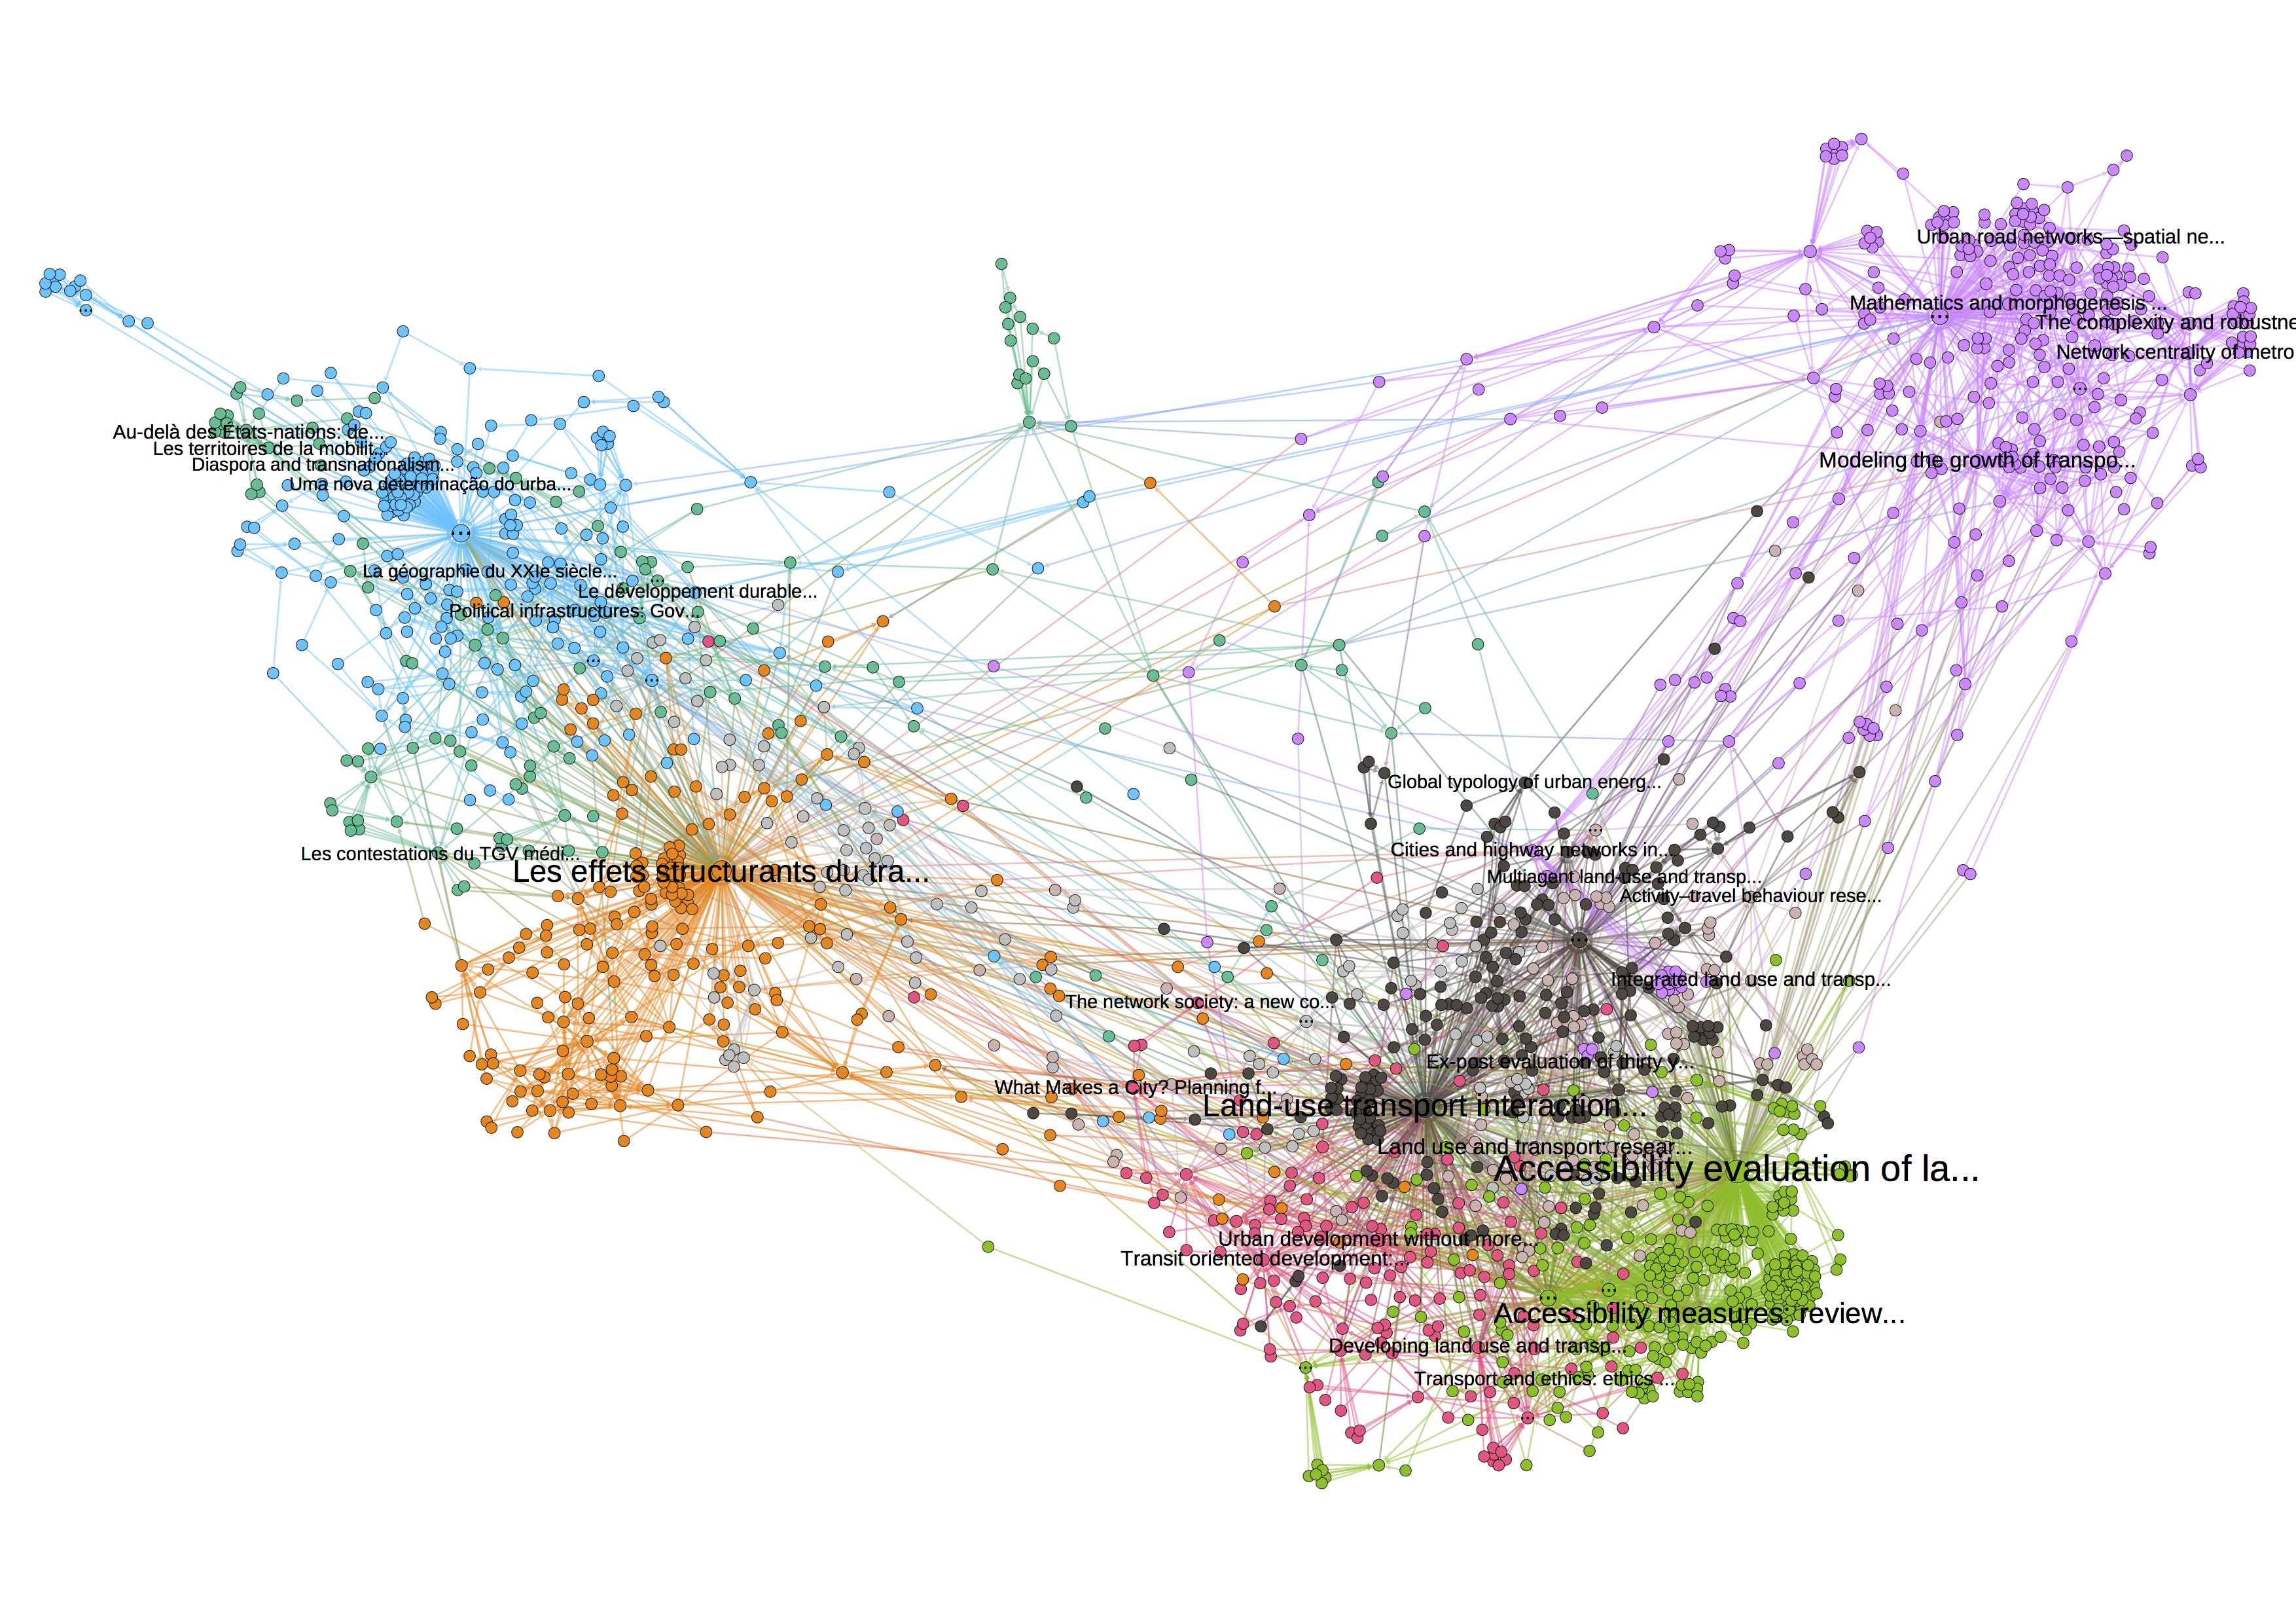
\includegraphics[width=\linewidth]{Figures/QuantEpistemo/rawcore}
\caption[Citation Network][Réseau de citations]{\textbf{Citation Network}\label{fig:quantepistemo:citnw}}{\textbf{Réseau de citations.} Nous visualisons les références ayant au moins deux liens, par un algorithme de force-atlas. Les couleurs donnent les communautés décrites dans le texte. En orange, bleu, turquoise: géographie urbaine, géographie des transports, sciences politiques ; en rose, noir, vert: planning, accessibilité, LUTI ; en violet : réseaux spatiaux (physique et économie).\label{fig:quantepistemo:citnw}}
\end{figure}
%%%%%%%%%%%%%%%%%





%%%%%%%%%%%%%%%%%%
\paragraph{Semantic Communities}{Communautés Sémantiques}


L'extraction des mots-clés est faite suivant une heuristique inspirée de~\cite{chavalarias2013phylomemetic}. La description complète de la méthode et de son implémentation est donnée en Appendice~\ref{app:sec:cybergeo}. Elle se base sur les relations au second ordre entre les entités sémantiques, qui sont des \emph{n-grams}, c'est à dire des mots-clés multiples pouvant avoir une longueur jusqu'à 3. Celles-ci sont estimées via la matrice de co-occurrence, dont les propriétés statistiques fournissent une mesure de déviation à des co-occurrences uniformes, qui est utilisée pour juger la pertinence des mots-clés. Sélectionnant un nombre fixe de mots-clés pertinents $K_W = 10000$, nous pouvons ensuite construire un réseau pondéré par les co-occurrences.


\bpar{
The topology of raw networks does not allow the extraction of clear communities, in particular because of the presence of hubs that correspond to frequent terms common to many fields (e.g. \texttt{model}, \texttt{space}). We assume these highest degree terms do not carry specific information on particular classes and can be thus filtered given a maximal degree threshold $k_{max}$. Similarly, edge with small weight are considered as noise and filtered according to a minimal edge weight threshold $\theta_w$. Keywords are preliminary filtered by a document frequency window $\left[ f_{min},f_{max} \right]$ which is slightly different from network filtering and complementary. A sensitivity analysis of resulting network topology to these parameters is presented in Fig.~\ref{fig:sensitivity}. We choose parameter values that maximize modularity under the constraint of a community number and size distribution of same magnitude as technological classes. This multi-objective optimization does not have a unique solution as objectives are somehow contradictory, and a compromise point must be chosen.
}{
La topologie du réseau brut ne permet pas l'extraction claire de communautés, en particulier à cause de hubs qui correspondent à des termes fréquents commun à de nombreux champs (e.g. \texttt{model}, \texttt{space})\comment[FL]{statut de ces mots ?}. Nous faisons l'hypothèse que ces termes à fort degré ne portent pas d'information particulière sur des classes données et peuvent ainsi être filtrés étant donné un seuil de degré maximal $k_{max}$ (on s'intéresse alors à ce qui fait la spécificité de chaque domaine). De la même manière, les liens avec un poids faibles sont considérés comme du bruit et filtrés selon un seuil de poids minimal $\theta_w$. La méthode générique permet de plus une filtration préliminaire des mot-clés, complémentaire à la filtration topologique, par fréquence d'apparition dans les documents $\left[ f_{min},f_{max} \right]$, à laquelle les résultats ne sont pas sensibles dans notre cas. L'analyse de sensibilité des caractéristiques du réseau filtré, notamment de sa taille, modularité et structure des communautés, est donnée en~\ref{app:sec:quantepistemo}. Nous choisissons des valeurs de paramètres permettant une optimisation multi-objectif entre modularité et taille du réseau, $\theta_w = 10,k_{max} = 500$, par le choix d'un point compromis sur un front de Pareto, qui donne un réseau sémantique de taille $(V=7063,E=48952)$. Celui-ci est visualisé en Appendice~\ref{app:sec:quantepistemo}.
}


\bpar{
We then retrieve communities in the semantic network (using standard Louvain algorithm, with the optimized filtering parameters). communities correspond to well-defined scientific fields (and/or domains, approaches). An expert validation allow us to give names to these, a more complicated naming procedure would eventually be possible (as in~\cite{yang2000improving} for the case of patents 
 where a chi-square test on distribution of documents in classes), but we prefer to stick here to a certain level of supervision. Table~\ref{tab:domains} summarizes the communities 
}{
Nous récupérons ensuite les communautés dans le réseau par un clustering de Louvain standard sur le réseau filtré optimal. On obtient 20 communautés pour une modularité de 0.58. Celles-ci sont examinées à la main pour être nommées, les techniques de désignation automatique~\cite{yang2000improving} n'étant pas assez élaborées et ne font pas la distinction implicite entre champs thématiques et méthodologiques par exemple (en fait entre les domaines de connaissance, voir~\ref{sec:knowledgeframework}) qui est une dimension supplémentaire que nous ne traitons pas ici, mais nécessaire pour avoir des désignations parlantes. Les communautés sont décrites en Table~\ref{tab:quantepistemo:semanticdomains}. On voit tout de suite la complémentarité avec l'approche par citation, puisque se dégagent ici à la fois des sujet d'étude (High Speed Rail, Maritime Networks), des domaines et méthodes (Networks, Remote Sensing, Mobility Data Mining), des domaines thématiques (Policy), des méthodes pures (Agent-based Modeling, Measuring). Ainsi, une référence peut mobiliser plusieurs de ces communautés. On a de plus une granularité plus fine de l'information. L'effet du langage est puissant puisque la géographie française se distingue en une catégorie séparée (des analyses poussées pourraient être envisagées pour mieux comprendre le phénomène et en tirer parti: sous-communautés, reconstruction d'un réseau spécifique, études par traduction ; mais celles-ci sont hors de propos dans cette étude exploratoire). On constante l'importance des réseaux, des problématiques de sciences politiques et socio-économiques. Nous mobiliserons la première catégorie dans la plupart des modèles développés, mais en gardant en tête l'importance des problématiques liées à la gouvernance, nous réaliserons un travail spécifique en~\ref{sec:lutetia}.
}




%%%%%%%%%%%%%%%%%%
\begin{table}
\caption[Semantic communities][Communautés sémantiques]{Disciplines/domains/fields reconstructed from community detection in the semantic network}{\textbf{Description des communautés sémantiques.} On donne leur taille, leur proportion en quantité de mots-clés cumulés sur l'ensemble du corpus, et des mots-clés représentatifs sélectionnés par degré maximal.\comment[FL]{pourquoi ces mots sont ils tronques ?}[(JR) cest explique dans le texte (surtout en annexe) il s'agit de stem]}
\label{tab:quantepistemo:semanticdomains}
\begin{tabular}{llll}
\hline\noalign{\smallskip}
Name & Size & Weight & Keywords  \\
\noalign{\smallskip}\hline\noalign{\smallskip}
Networks & 820 & 13.57\% & \texttt{social network, spatial network, resili} \\
Policy & 700 & 11.8\% & \texttt{actor, decision-mak, societi} \\
Socio-economic & 793 & 11.6\% & \texttt{neighborhood, incom, live} \\
High Speed Rail & 476 & 7.14\% & \texttt{high-spe, corridor, hsr} \\
French Geography & 210 & 6.08\% & \texttt{système, développement, territoire} \\
Education & 374 & 5.43\% & \texttt{school, student, collabor} \\
Climate Change & 411 & 5.42\% & \texttt{mitig, carbon, consumpt} \\
Remote Sensing & 405 & 4.65\% & \texttt{classif, detect, cover} \\
Sustainable Transport & 370 & 4.38\% & \texttt{sustain urban, travel demand, activity-bas} \\
Traffic & 368 & 4.23\% & \texttt{traffic congest, cbd, capit} \\
Maritime Networks & 402 & 4.2\% & \texttt{govern model, seaport, port author} \\
Environment & 289 & 3.79\% & \texttt{ecosystem servic, regul, settlement} \\
Accessibility & 260 & 3.23\% & \texttt{access measur, transport access, urban growth} \\
Agent-based Modeling & 192 & 3.18\% & \texttt{agent-bas, spread, heterogen} \\
Transportation planning & 192 & 3.18\% & \texttt{transport project, option, cba} \\
Mobility Data Mining & 168 & 2.49\% & \texttt{human mobil, movement, mobil phone} \\
Health Geography & 196 & 2.49\% & \texttt{healthcar, inequ, exclus} \\
Freight and Logistics & 239 & 2.06\% & \texttt{freight transport, citi logist, modal} \\
Spanish Geography & 106 & 1.26\% & \texttt{movilidad urbana, criteria, para} \\
Measuring & 166 & 1.0\% & \texttt{score, sampl, metric} \\
\noalign{\smallskip}\hline
\end{tabular}
\end{table}
%%%%%%%%%%%%%%%%%%



%%%%%%%%%%%%%%%%%%
\paragraph{Measures of Interdisciplinarity}{Mesures d'interdisciplinarité}


\bpar{
Distribution of keywords within communities provides an article-level interdisciplinarity.
Combination of citation and semantic layers in the hyper-network provide second order interdisciplinarity measures, that we don't use here because of the modest size of the citation network. More precisely, a reference can be viewed as a probability vector on semantic classes.
}{
La distribution des mots clés dans les communautés permettent de définir une mesure d'interdisciplinarité au niveau de l'article. La combinaison des couches de citation et sémantique dans l'hyperréseau fournit des mesures d'interdisciplinarité au second ordre (motifs sémantiques des cités ou des citants), que nous n'utiliserons pas ici à cause de la taille modeste du réseau de citation (voir \ref{app:sec:cybergeo} et \ref{app:sec:patents}). Plus précisément, une référence $i$ peut être vue comme un vecteur de probabilités sur les classes sémantiques $j$, qu'on notera sous forme matricielle $\mathbf{P}=(p_{ij})$. Celles-ci sont estimées simplement par les proportions de mots-clés classifiés dans chaque classe pour la référence. Une mesure classique d'interdisciplinarité~\cite{bergeaud2017classifying} est alors $I_i = 1 - \sum_j p_{ij}^2$. Soit $\mathbf{A}$ la matrice d'adjacence du réseau de citation, et soit $\mathbf{I}_k$ les matrices de selection des lignes correspondants à la classe $k$ de la classification de citation: $Id\cdot \mathbbm{1}_{c(i)=k}$, telle que $I_k \cdot A \cdot I_{k'}$ donne exactement les citations de $k$ vers $k'$. La proximité de citation entre les communautés de citation est alors définie par $c_{kk'} = \sum \mathbf{I}_k \cdot \mathbf{A} \cdot \mathbf{I}_{k'} /  \sum \mathbf{I}_k \cdot \mathbf{A}$. On définit la proximité sémantique en définissant une matrice de distance entre références par $\mathbf{D} = d_{ii'}=\sqrt{\frac{1}{2}\sum (p_{ij}-p{i'j})^2}$ puis la proximité sémantique par $s_{kk'} = \mathbf{I}_k \cdot \mathbf{D} \cdot \mathbf{I}_{k'} / \sum \mathbf{I}_k \sum \mathbf{I}_{k'}$. Nous montrons en Fig.~\ref{fig:quantepistemo:interdisc} les valeurs de ces différentes mesures, ainsi que la composition sémantique des communautés de citation, pour les classes sémantiques majoritaires. La distribution de $I_i$ montre que les papiers gravitant dans le domaine du LUTI sont les plus interdisciplinaires dans les termes utilisés, ce qui pourrait être lié à leur caractère appliqué. Les autres disciplines sont dans des motifs similaires, à part la géographie et la planification des infrastructures qui présentent des distributions quasi-uniformes, témoignant de l'existence de références très spécialisées dans ces classes. Ce n'est pas nécessairement étonnant vu les sous-champs pointus exhibés (sciences politiques par exemples, et de même les études prospectives type coût-bénéfices sont très étriquées). Ce premier croisement des couches nous confirme les spécificités de chaque champ. Concernant les compositions sémantiques, la plupart agissent comme validation externe vu les classes majoritaires. Le champ le moins concerné par les problème socio-économiques est la planification des infrastructure, ce qui donnera du grain à moudre aux détracteurs de la technocratie. Les questions de changement climatique et durabilité sont relativement bien répartie. Enfin, les ouvrages géographiques concernent en majorité des problèmes de gouvernance. Les matrices de proximité confirment la conclusion de la sous-section précédente en terme de citation, les partages étant très faibles, les plus hautes valeurs étant jusqu'à un quart de la planification vers la géographie et des LUTI vers le TOD (mais pas l'inverse, les relations peuvent être à sens unique). Hors, les proximités sémantiques montrent par exemple que LUTI, TOD, Accessibility et Networks sont proches dans leur termes, ce qui est logique pour les trois premiers, et confirme pour le dernier que les physiciens se basent majoritairement sur les méthodes des ces champs liés au planing pour légitimer leur travaux. La géographie est totalement isolée, sa plus proche voisine étant la planification des infrastructures. Cette étude est très utile pour notre propos, puisqu'elle montre des domaines cloisonnés partageant des termes at donc a priori des problématiques et sujet commun. On ne se parle pas alors qu'on parle des languages pas si lointains, d'où la pertinence accrue de les faire parler d'une commune voie dans nos travaux : nos modèles devront mobiliser des éléments, ontologies et échelles de ces différents champs.
}



%%%%%%%%%%%%%%%%%%
\begin{figure}
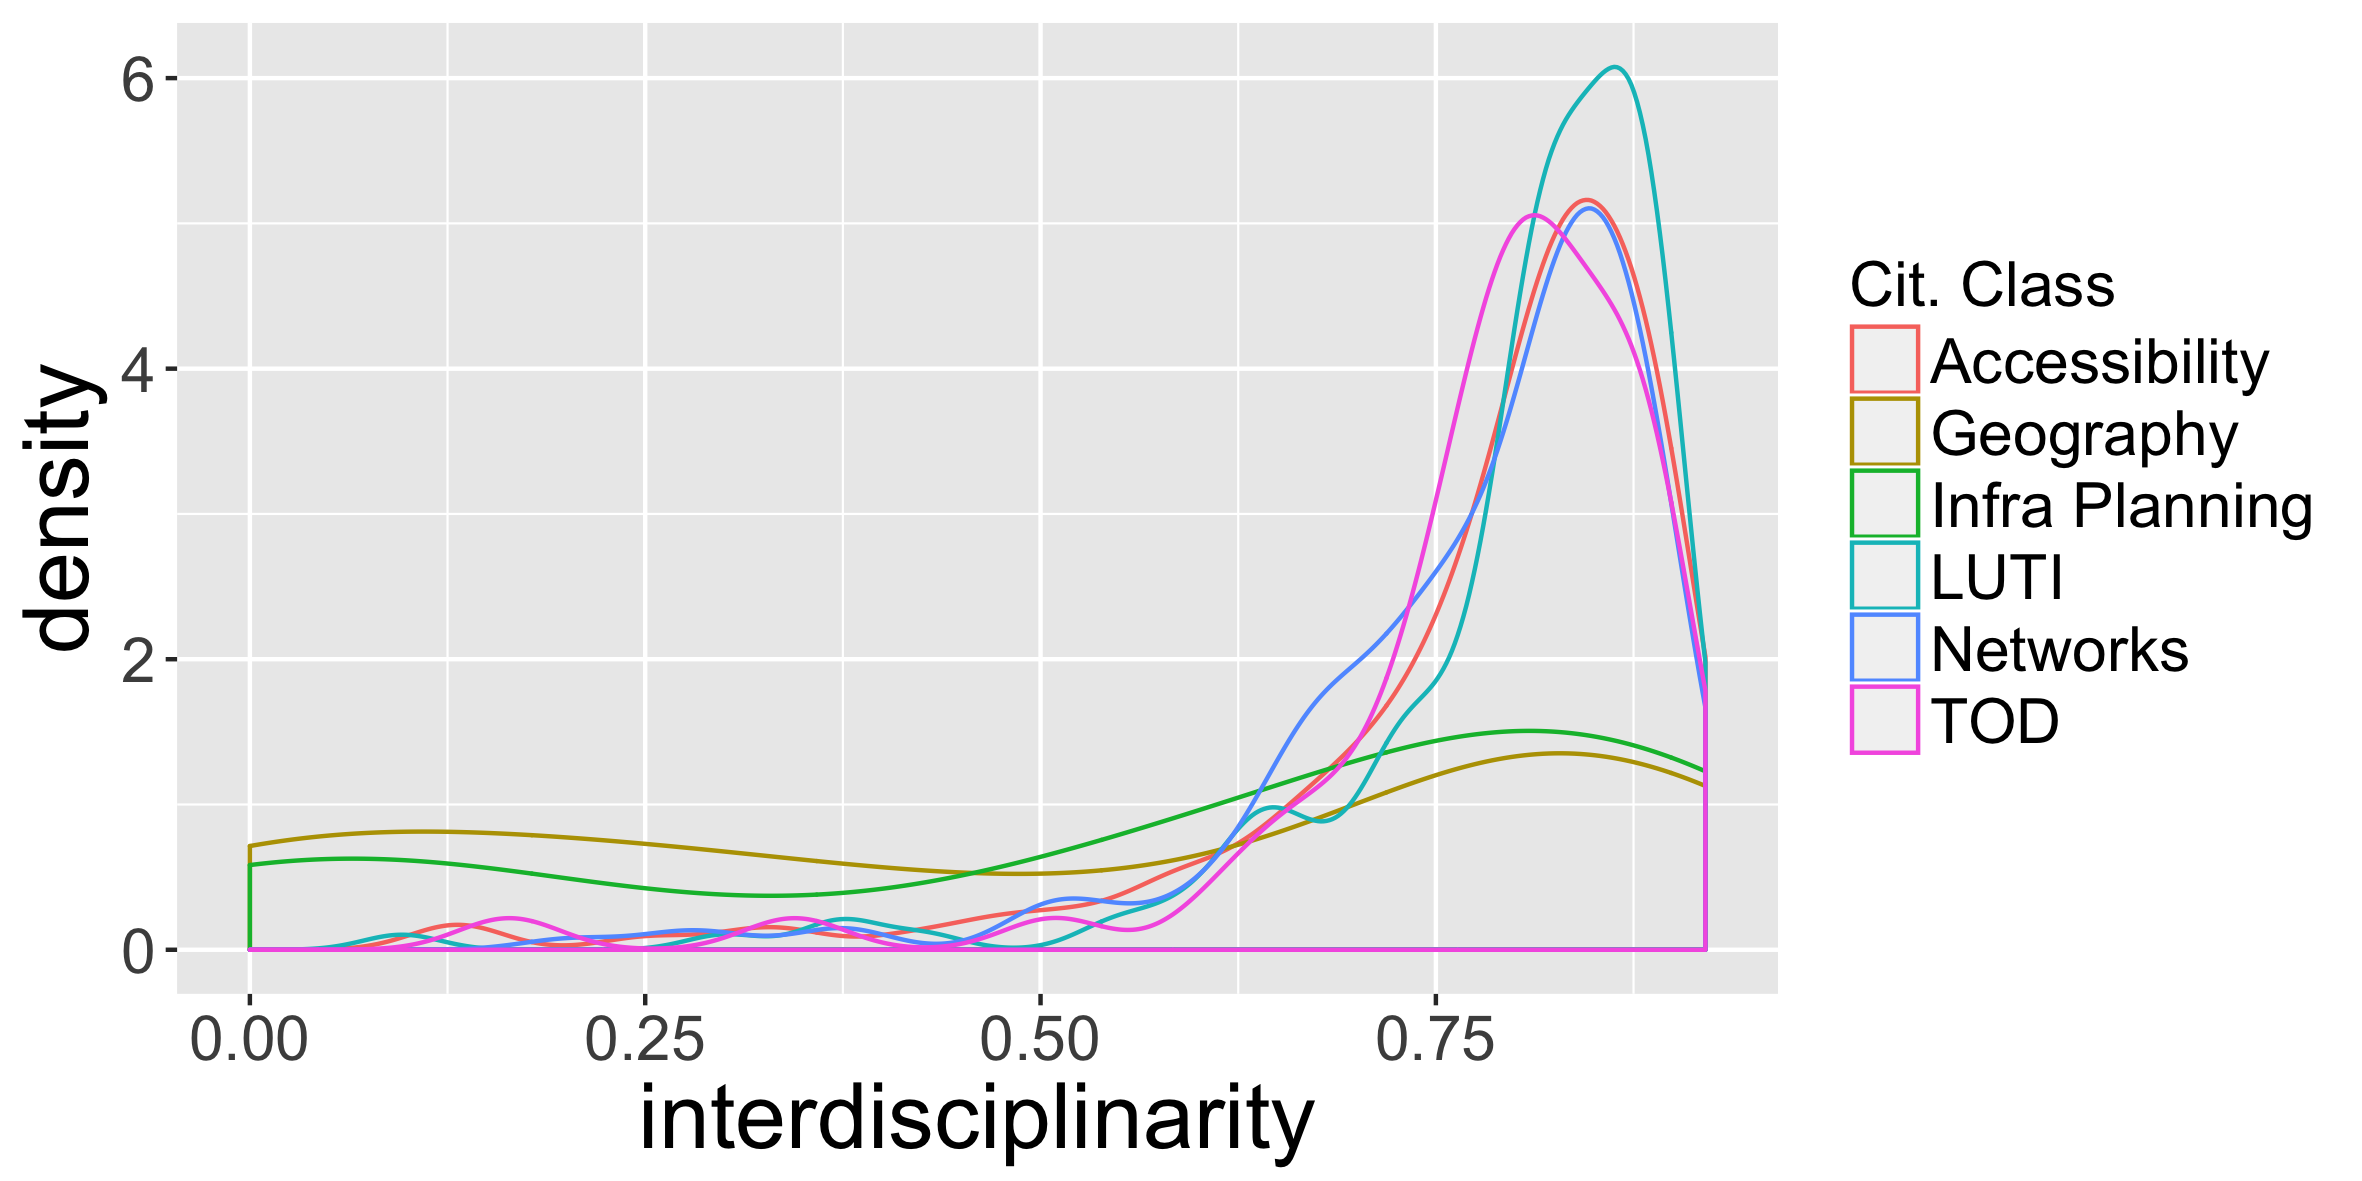
\includegraphics[width=0.49\linewidth]{Figures/QuantEpistemo/interdisciplinarities}
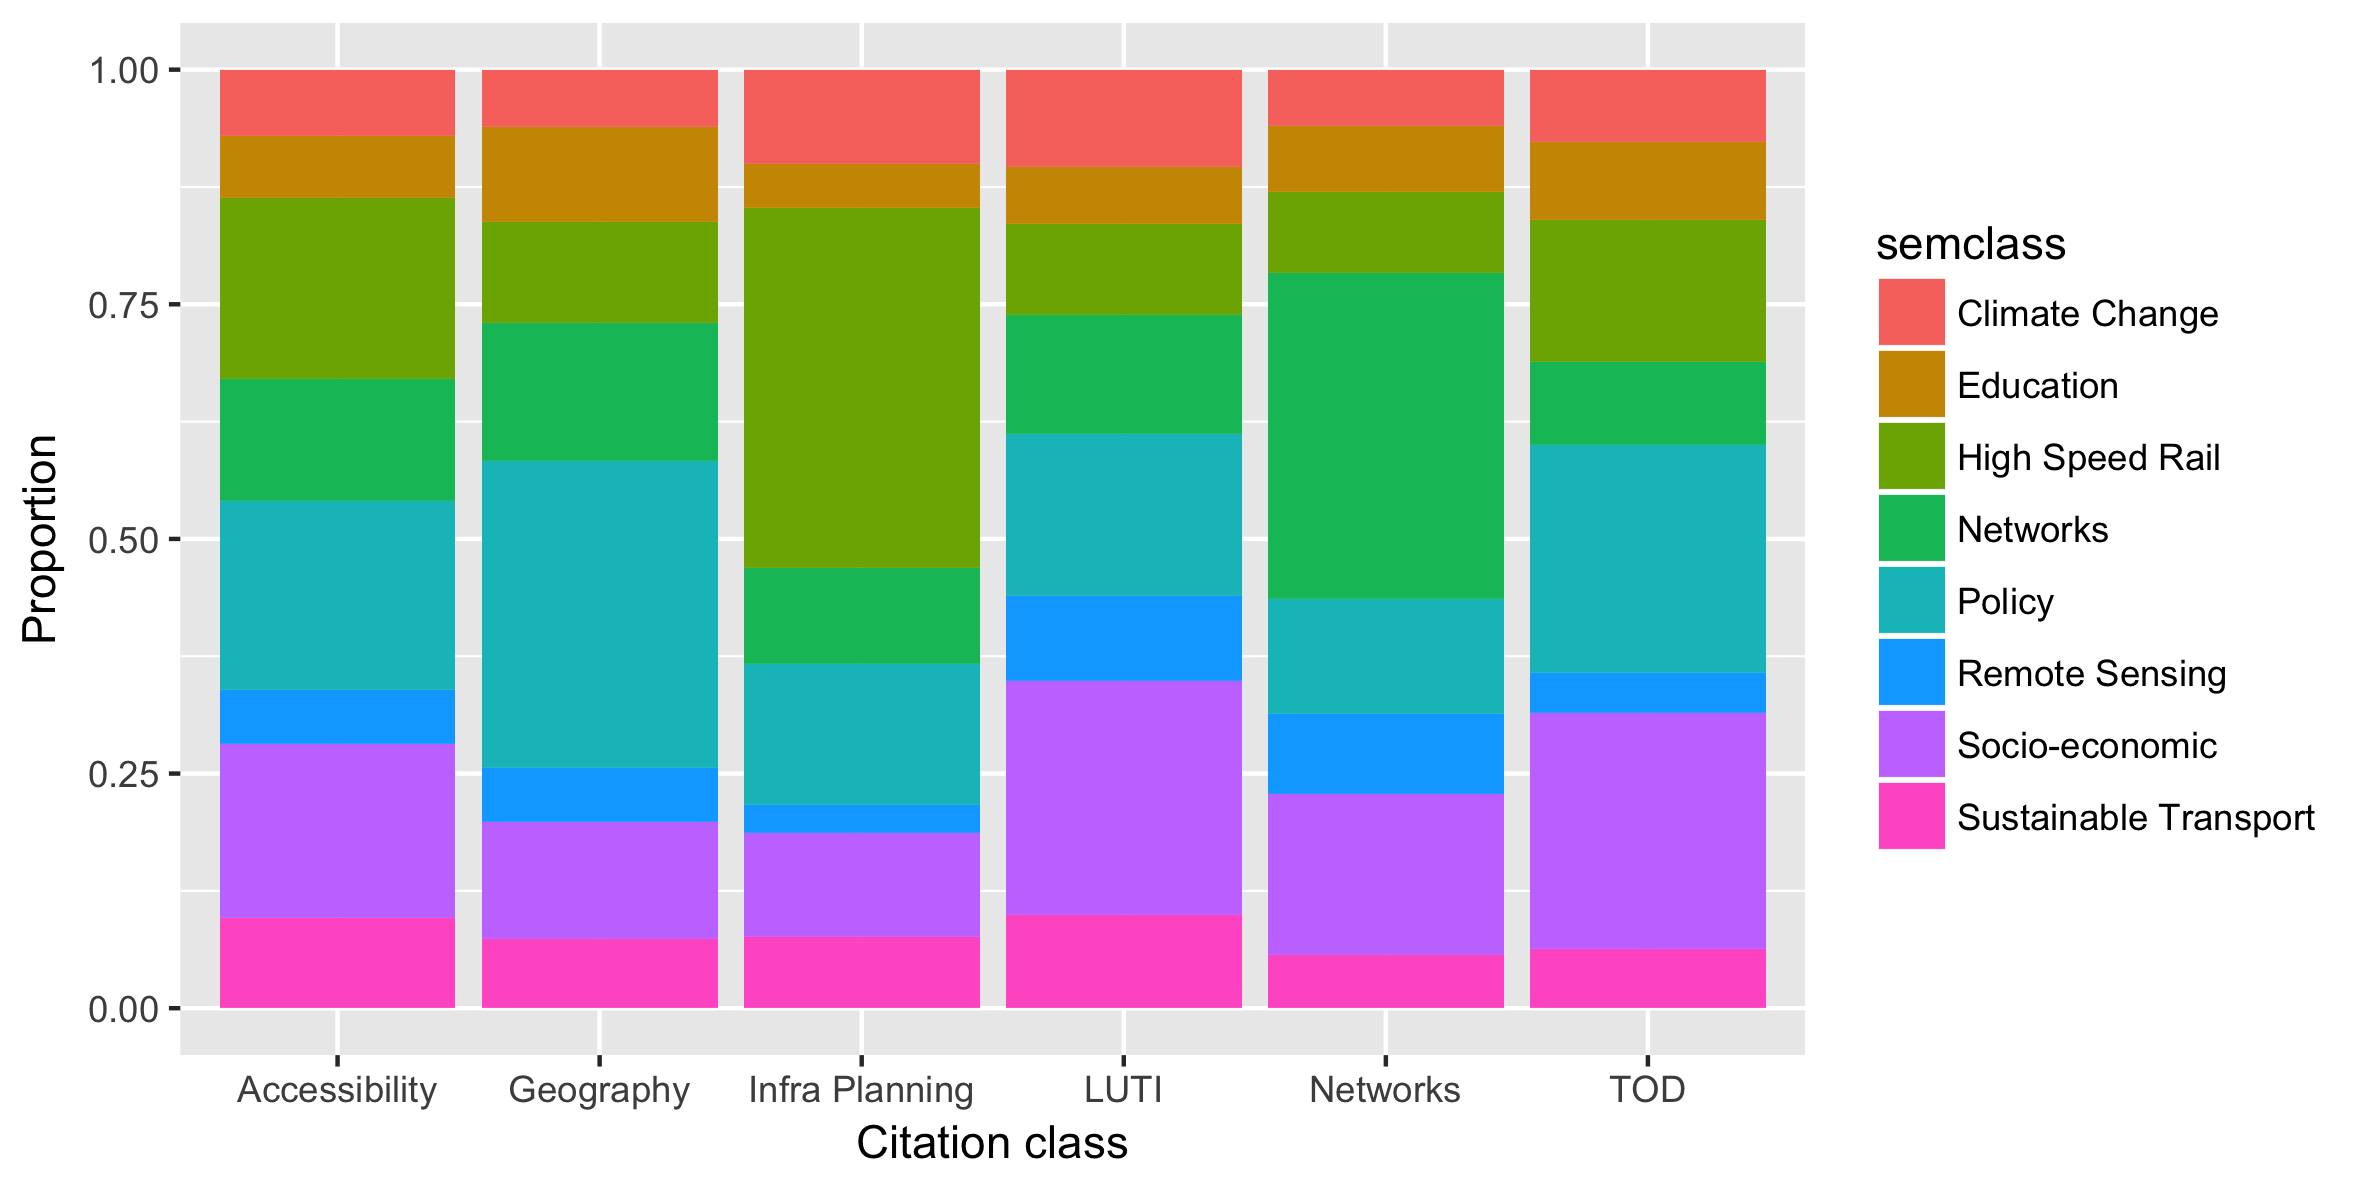
\includegraphics[width=0.49\linewidth]{Figures/QuantEpistemo/compo_proportion}\\
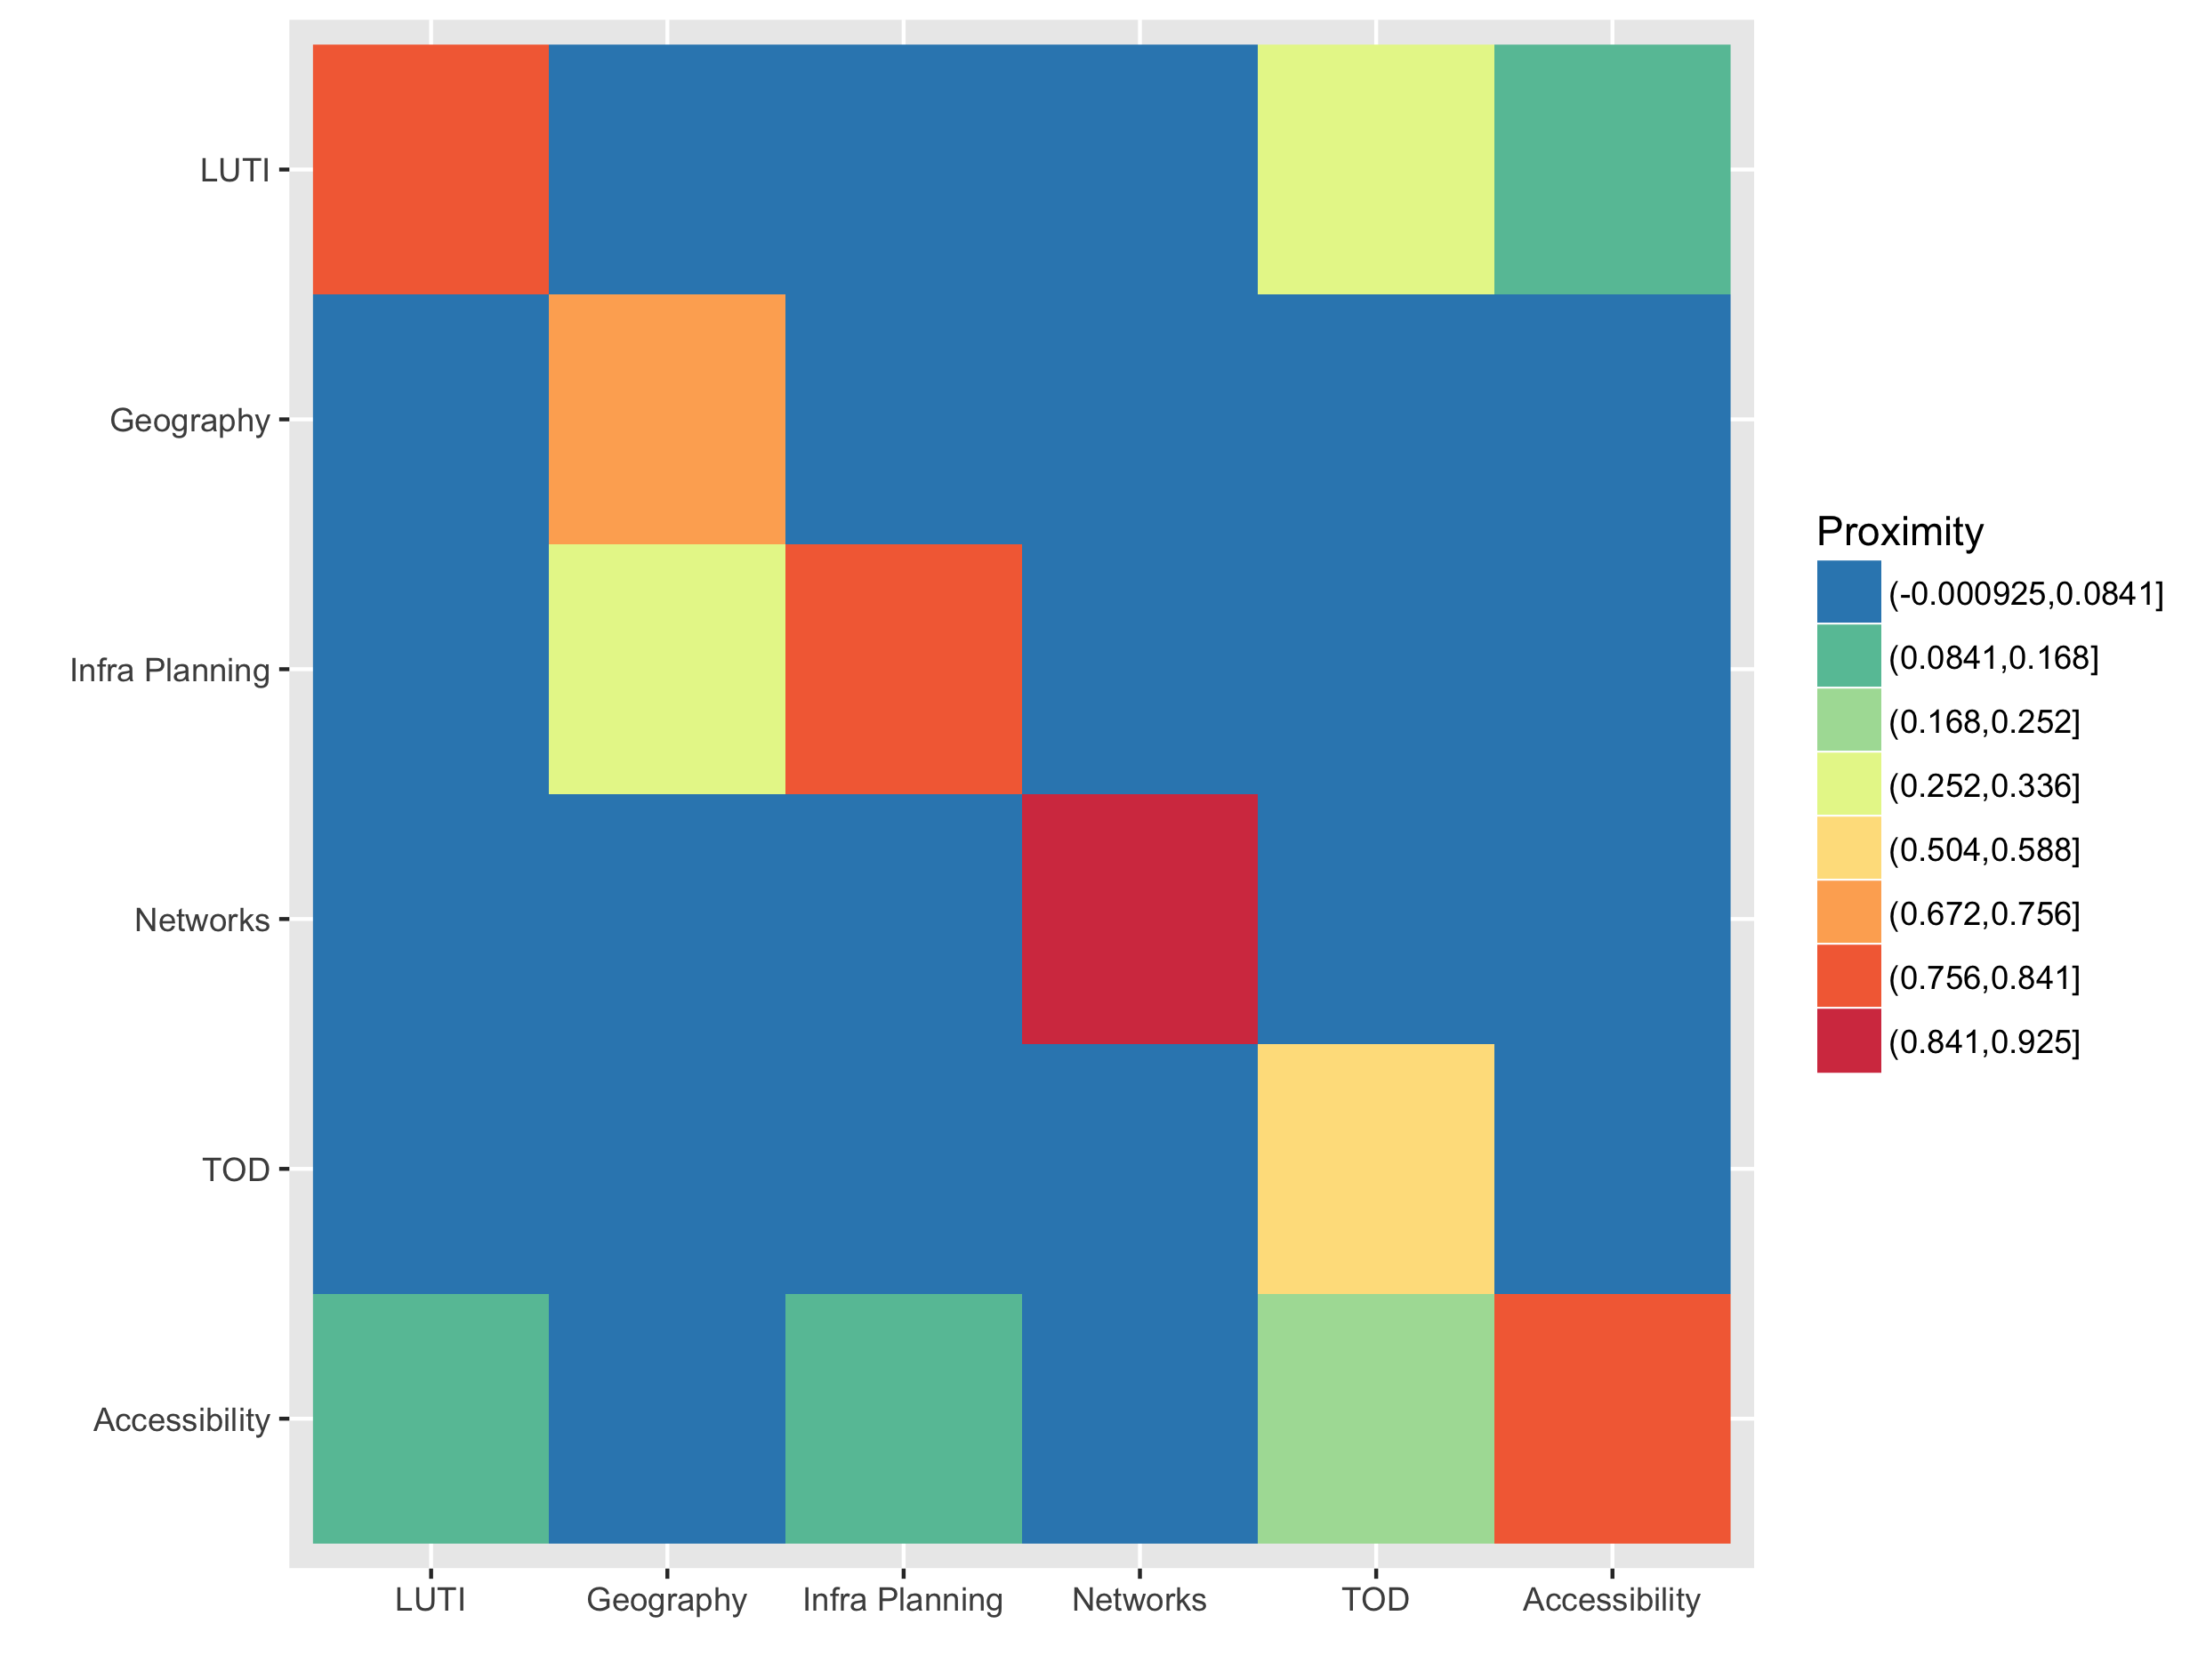
\includegraphics[width=0.49\linewidth]{Figures/QuantEpistemo/citation_proximities}
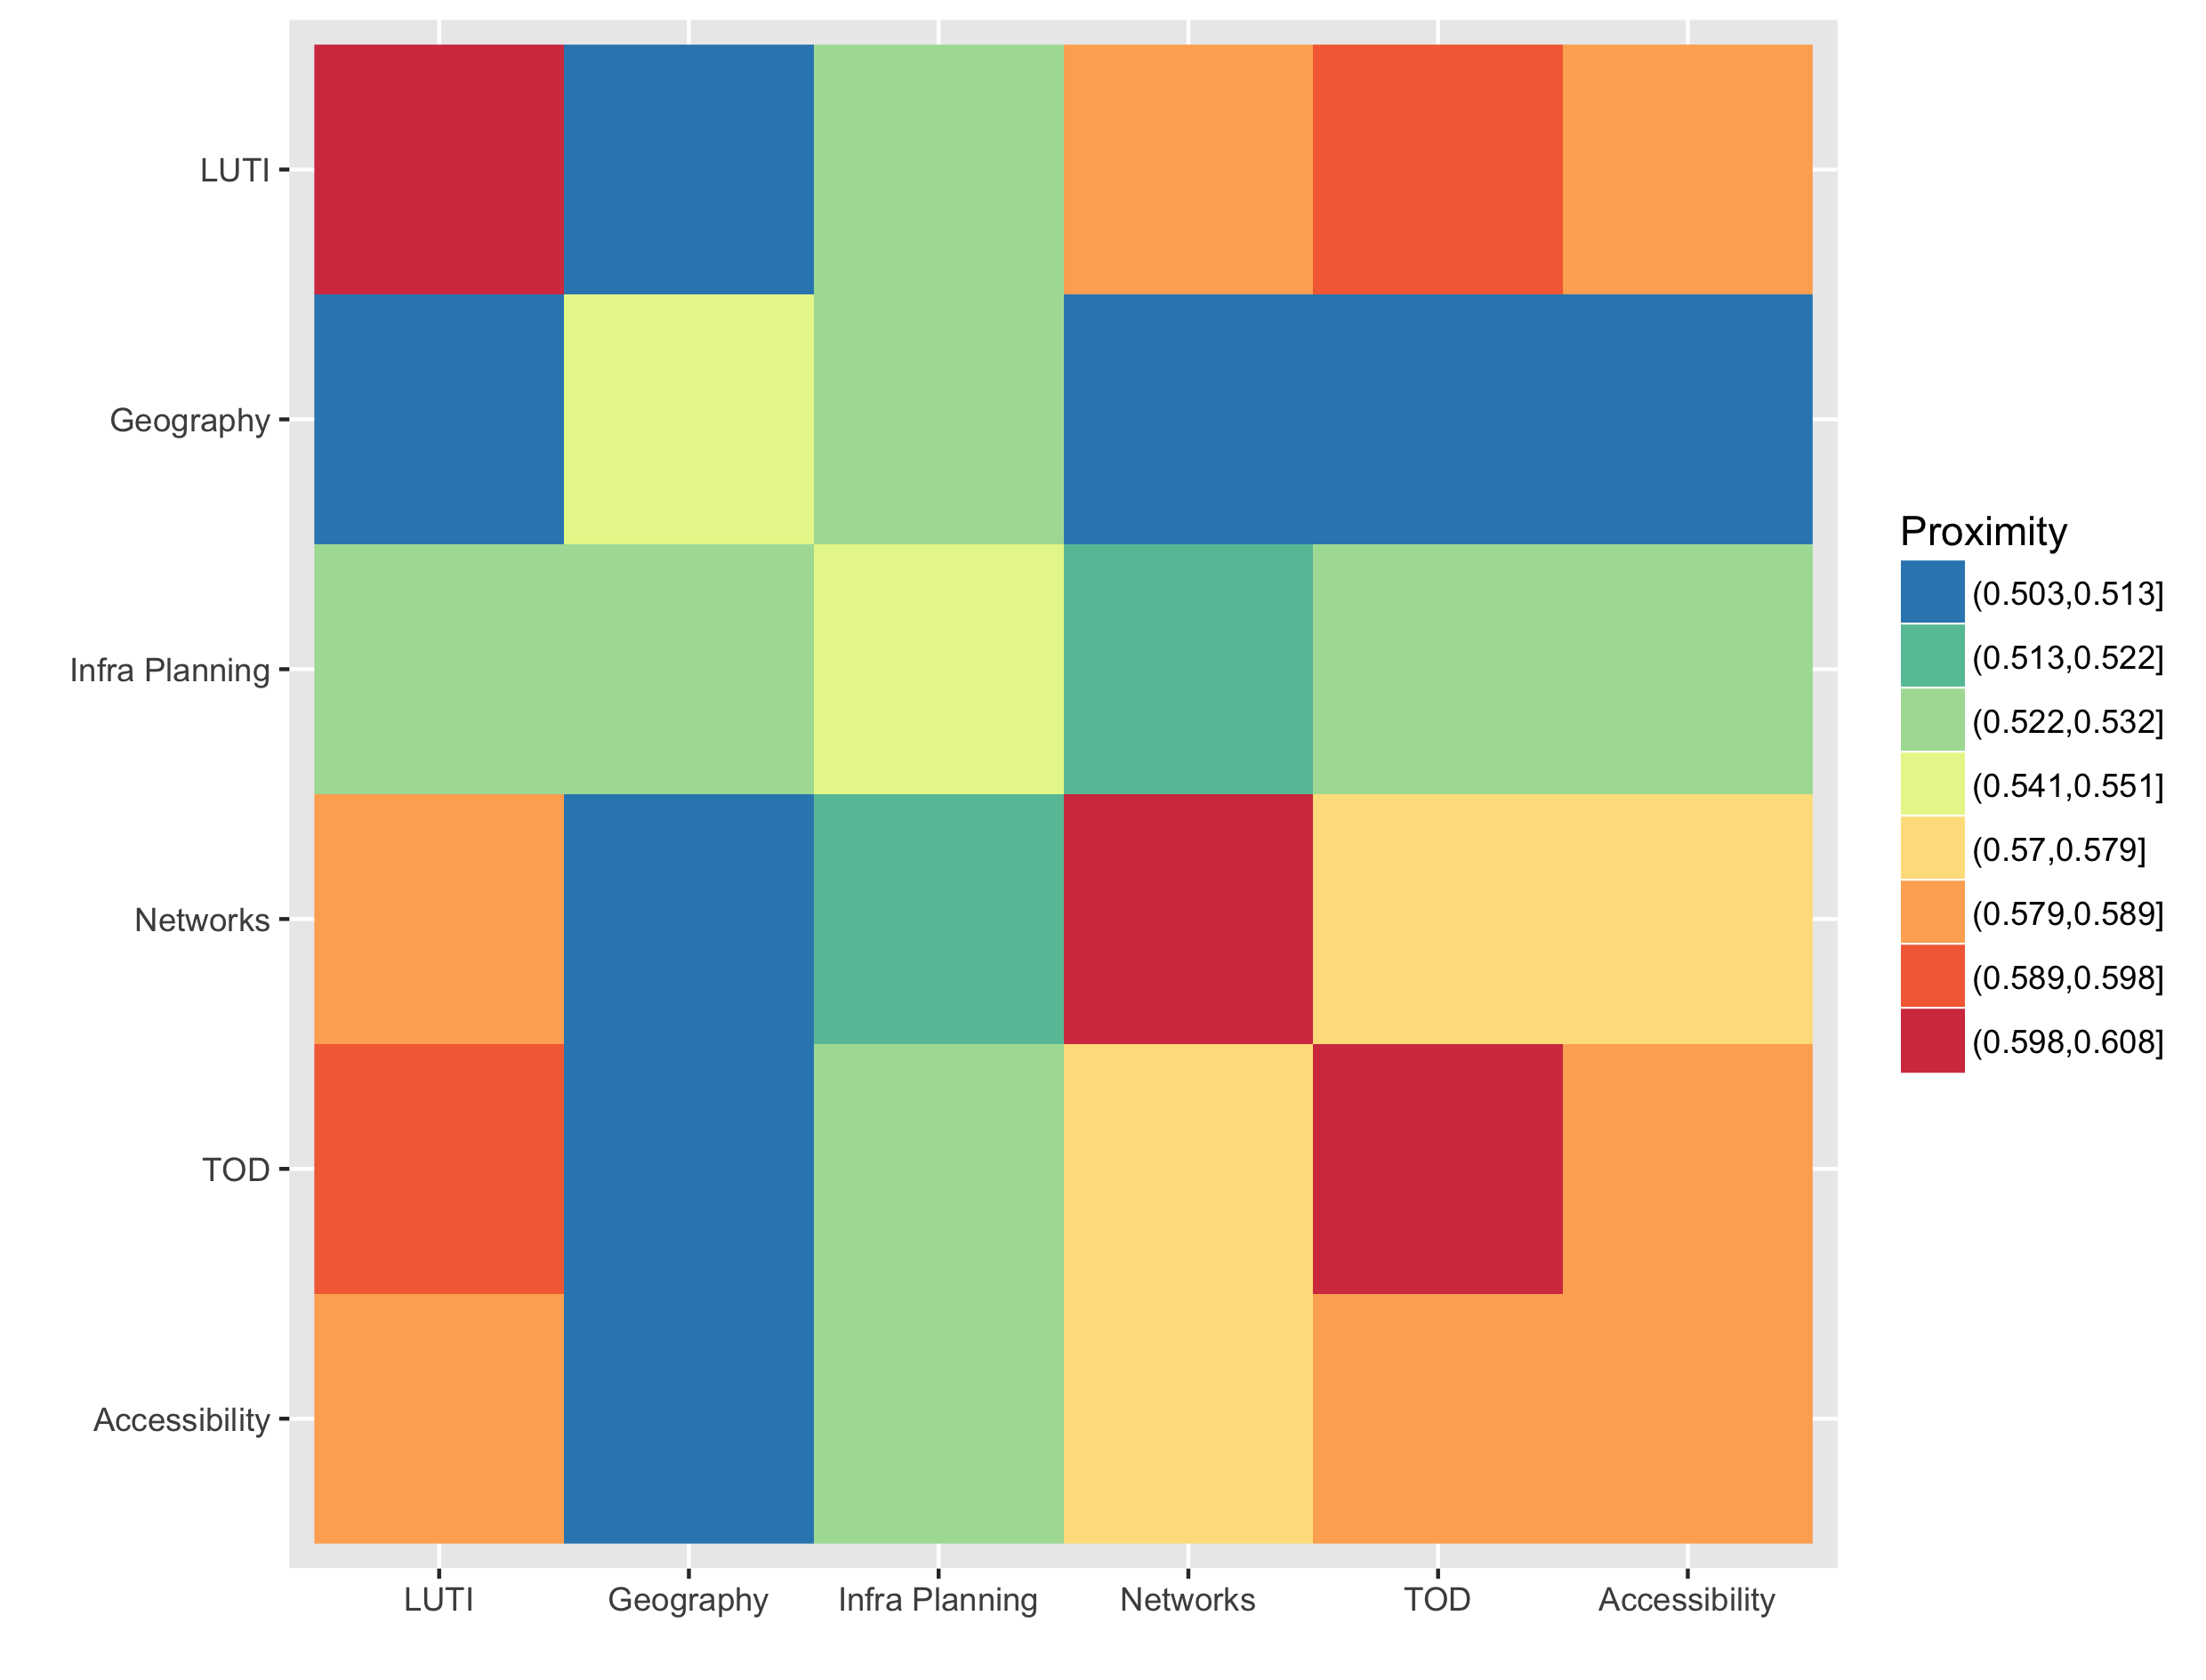
\includegraphics[width=0.49\linewidth]{Figures/QuantEpistemo/semantic_proximities}
\caption[][Motifs d'interdisciplinarité]{\label{fig:quantepistemo:interdisc}}{\textbf{Motifs d'interdisciplinarité.} \textit{(Haut Gauche)} Distribution des $I_i$ par classes de citations ; \textit{(Haut Droite)} Composition sémantiques des classes de citation ; \textit{(Bas Gauche)} Matrice de proximité de citation $c_{kk'}$ entre classes de citations ; \textit{(Bas Droite)} Matrice de proximité sémantique $s_{kk'}$ entre classes de citations.\label{fig:quantepistemo:interdisc}\comment[FL]{tu compares les disciplines entre elles mais pas la facon dont elles attaquent les questions au coeur de ta these. c'est dommage.}[(JR)c'est l'objet de la section suivante]}
\end{figure}
%%%%%%%%%%%%%%%%%%



% bootstrap
%min(corrs);max(corrs);mean(abs(corrs))
% -0.170952  0.5496791  0.08384802
% apply(bcorrs,2,mean)
%       minrho        maxrho    meanabsrho     minrhosup     maxrhosup meanabsrhosup 
%  -0.08792137    0.11690677    0.03137750   -0.17686637    0.68579406    0.11079253 
% apply(bcorrs,2,sd)
%       minrho        maxrho    meanabsrho     minrhosup     maxrhosup meanabsrhosup 
%  0.012683338   0.021324056   0.002250636   0.038402781   0.134996447   0.051553244 

% modularities
% sem : 0.1053156
% cit : 0.8140818
% bootstrap N=100
% sem : 0.073097051446193 +- 0.00307154703966512
% cit : 0.204223565075042 +- 0.0141450119581389


\bpar{
}{
Nous concluons cette analyse par une approche plus robuste pour quantifier les proximités entre couches de l'hyperréseau. Il est aisé de construire une matrice de corrélation entre deux classifications, par les corrélations de leur colonnes. Nous définissons les probabilités $\mathbf{P}_C$ toutes égales à 1 pour la classification de citation. La matrice de correlation de celle-ci avec $\mathbf{P}$ s'étend de -0.17 à 0.54 et a une moyenne de valeur absolue de 0.08, ce qui est significatif par rapport à des classifications aléatoire puisque un bootstrap à $b=100$ répétitions avec les matrices mélangées donne un minimum à $-0.08 \pm 0.012$, un maximum à $0.11 \pm 0.02$ et une moyenne absolue à $0.03 \pm 0.002$. Cela montre que les classifications sont complémentaires et que cette complémentarité est significative statistiquement par rapport à des classifications aléatoires. L'adéquation de la classification sémantique par rapport au réseau de citation peut également être quantifiée par la modularité multi-classes~\cite{nicosia2009extending} (voir~\ref{sec:app:patents} pour une définition mathématique), qui traduit la probabilité qu'un lien soit dû à la classification étudiée, en prenant en compte l'appartenance simultanée à de multiples classes. Ainsi, la modularité multi-classes des probabilités sémantiques pour le réseau de citation est de 0.10, ce qui d'une part est significativement signe d'adéquation, un bootstrap toujours à $b=100$ donnant une valeur de $0.073 \pm 0.003$, qui reste limitée vu la valeur maximale fixée par les probabilités de citations dans leur propre réseau qui donnent une valeur de 0.81, ce qui confirme d'autre part la complémentarité des classifications.
}








%--------------------------------------------------------------



%%%%%%%%%%%%%%%%%%%%%%%%
\subsection{Discussion}{Discussion}




\subsubsection{Towards modeling purpose and context automatic extraction}{Vers une modélisation des thèmes et une extraction automatique du contexte}


\bpar{
A possible direction to strengthen our quantitative epistemological analysis would be to work on full textes related to the modeling of interaction between networks and territories, with the aim to automatically extract thematics within articles. The idea would be to perform some kind of automatized modelography, with possible features to be extracted that would be ontologies, model architecture or structures, scales, or even typical parameter values. It is not clear to what degree structure of models can be extracted from their description in papers and it surely depends on the discipline considered. For example in a framed field such as transportation planning, using a pre-defined ontology (in the sense of dictionary) and a fuzzy grammar could be efficient to extract information as the discipline is relatively formatted. In theoretical and quantitative geography, beyond the barrier of language, information organisation is surely less subject to unsupervised data-mining because of the more literary nature of the discipline : synonyms and figures of speech are generally the norm in good level human sciences writing, fuzzing a possible generic structure of knowledge description. 
}{
Une direction possible pour renforcer cette analyse en épistémologie quantitative serait de travailler sur les textes complets des références contenant des efforts de modélisations des interactions entre réseaux et territoires, avec le but d'extraire automatiquement les thématiques des articles. Des méthodes plus adaptées pour les long texte que celle utilisée ici incluent par exemple l'Allocation Latente de Dirichlet~\cite{blei2003latent}. L'idée serait de procéder à une sorte de modélographie automatique, pour extraire des caractéristiques telle les ontologies, l'architecture ou la structure des modèles, les échelles ou même des valeurs typiques des paramètres. Il n'est pas clair dans quelle mesure la structure des modèles peut être extraite de leur description dans un article, et cela dépend sûrement de la discipline considérée. Par exemple dans champ relativement cadré comme la planification des transports, l'utilisation d'une ontologie pré-définie (dans le sens d'un dictionnaire) et d'une grammaire floue pourrait être efficace vu les conventions assez strictes dans la discipline. En géographie théorique et quantitative, au delà de la barrière du language\comment[FL]{?}, l'organisation de l'information est sûrement plus délicate à appréhender par de l'apprentissage non-supervisé à cause de la nature plus littéraire de la discipline : les synonymes et les figures de style sont généralement la norme pour l'écriture d'un bon niveau en sciences humaines, rendant plus floue une possible structure générique de la description des connaissances.
}


%Depending on extended results of the two previous sections and on thematic requirements (huge need of knowledge on precise models structure, that may appear when trying to construct more specialized operational models), this project may be conducted with more or less investment.




\subsubsection{Reflexivity}{Réflexivité}


\bpar{
The methodology developed here is particularly interesting since it is reflexive, i.e. it can be used on our work itself. Therefore, an other application will be the reflexivity of our thesis : we attend to proceed to similar analysis on our proper bibliography (and possibly its evolution, available via \texttt{git} history), to understand our patterns of knowledge, possible gaps or unveil unexpected developments. The detailed development is done in Appendix~\ref{app:reflexivity}.
}{
La méthodologie que nous avons développé ici est particulièrement intéressante puisqu'elle offre des potentialités de réflexivité, c'est à dire qu'elle peut être utilisée pour étudier notre approche elle-même. Une de ses applications, hors de celle à la revue scientifique Cybergeo dans la perspective de Science Ouverte (voir Appendice~\ref{app:sec:cybergeo}), sera à notre propre corpus de références, dans le but de révéler des possibles  directions de recherche ou problématiques exotiques. Il est éventuellement possible de le faire de manière dynamique, grâce à l'historique de \texttt{git} qui permet de récupérer n'importe quelle version de la bibliographie à une date donnée sur les trois ans écoulés. Il s'agira aussi de comprendre nos motifs de production de connaissance afin de contribuer à~\ref{sec:knowledgeframework}. Le développement détaillé est fait en Appendice~\ref{app:reflexivity}.
}





\stars




%%%%%%%%%%%%%%%%%%%%%%%%%%%%%





\cleardoublepage % Empty page before the start of the next part

%------------------------------------------------

\ctparttext{This part aims at producing knowledge from the empirical analysis of case studies and from first modeling experiments. Explicit testing of hypothesis drawn from the theory is not achieved yet as these are preliminary steps for a reasoned insight into empirical and modeling domains.} % Text on the Part 2 page describing the content in Part 2


% Part II : Empirical analysis / Toy-modeling
% TODO : part 2 should set up the elementary bricks for further work ?
%\part{Modeling and Empirical Analysis} % Second part of the thesis
\part{Architecture and Building Bricks : preparing the construction}




%%%%%%%%%%%%%%%
% Transportation Equilibrium
%  -> first insight at a micro scale, from empirical point of view


\newpage

%----------------------------------------------------------------------------------------


\section[Static User Equilibrium][Equilibre Utilisateur Statique]{Investigating the Empirical Existence of Static User Equilibrium}{Investigation Empirique de l'Existence de l'Equilibre Utilisateur Statique}

\label{sec:transportationequilibrium}



%----------------------------------------------------------------------------------------


\bpar{
The Static User Equilibrium is a powerful framework for the theoretical study of traffic. Despite the restricting assumption of stationary flows that intuitively limit its application to real traffic systems, many operational models implementing it are still used without an empirical validation of the existence of the equilibrium. We investigate its existence on a traffic dataset of three months for the region of Paris, FR. The implementation of an application for interactive spatio-temporal data exploration allows to hypothesize a high spatial and temporal heterogeneity, and to guide further quantitative work. The assumption of locally stationary flows is invalidated in a first approximation by empirical results, as shown by a strong spatial and temporal variability in shortest paths and in network topological measures such as betweenness centrality. Furthermore, the behavior of spatial autocorrelation index of congestion patterns at different spatial ranges suggest a chaotic evolution at the local scale, especially during peak hours. We finally discuss the implications of these empirical findings and describe further possible developments based on the estimation of Lyapunov dynamical stability of traffic flows.
}{
L'Equilibre Utilisateur Statique est un cadre puissant pour l'étude théorique du trafic. Malgré l'hypothèse restreignante\comment[FL]{de quel point de vue ?} de stationnarité des flots qui intuitivement limite son application aux systèmes de trafic réels, de nombreux modèles opérationnels qui l'implémentent sont toujours utilisés sans validation empirique de l'existence de l'équilibre. Nous étudions celle-ci sur un jeu de données de trafic couvrant trois mois sur la région parisienne. L'implémentation d'une application d'exploration interactive de données spatio-temporelles permet de formuler l'hypothèse d'une forte hétérogénéité spatiale et temporelle, guidant les études quantitatives. L'hypothèse de flots localement stationnaires est invalidée en première approximation par les résultats empiriques, comme le montrent une forte variabilité spatio-temporelle des plus courts chemins et des mesures topologiques du réseau comme la centralité de chemin. De plus, le comportement de l'index d'autocorrelation spatiale pour les motifs de congestion à différentes portées spatiales suggère une évolution chaotique à l'échelle locale, en particulier lors des heures de pointe. Nous discutons finalement les implications de ces résultats empiriques et proposons des possibles développements futurs basés sur l'estimation de la stabilité dynamique au sens de Lyapounov des flots de trafic.
}


%%%%%%%%%%%%%%%%%%%%%%%
\subsection{Context}{Contexte}
\label{treq:introduction}


\bpar{
Traffic Modeling has been extensively studied since seminal work by~\cite{wardrop1952road} : economical and technical elements at stake justify the need for a fine understanding of mechanisms ruling traffic flows at different scales. Many approaches with different purposes coexist today, of which we can cite dynamical micro-simulation models, generally opposed to equilibrium-based techniques. Whereas the validity of micro-based models has been largely discussed and their application often questioned, the literature is relatively poor on empirical studies assessing the stationary equilibrium assumption in the Static User Equilibrium (SUE) framework. Various more realistic developments have been documented in the literature, such as Dynamic Stochastic User Equilibrium (DSUE) (see e.g. a description by~\cite{han2003dynamic}). An intermediate between static and stochastic frameworks is the Restricted Stochastic User Equilibrium, for which route choice sets are constrained to be realistic (\cite{rasmussen2015stochastic}). Extensions that incorporate user behavior with choice models have more recently been proposed, such as~\cite{zhang2013dynamic} taking into account both the influence of road pricing and congestion on user choice with a Probit model. Relaxations of other restricting assumptions such as pure user utility maximization have been also introduced, such as the Boundedly Rational User Equilibrium described by~\cite{mahmassani1987boundedly}. In this framework, user have a range of satisfying utilities and equilibrium is achieved when all users are satisfied. It produces more complex features such as the existence of multiple equilibria, and allows to account for specific stylized facts such as irreversible network change as developed by~\cite{guo2011bounded}. Other models for traffic assignment, inspired from other fields have also recently been proposed : in~\cite{puzis2013augmented}, an extended definition of betweenness centrality combining linearly free-flow betweenness with travel-time weighted betweenness yield a high correlation with effective traffic flows, acting thus as a traffic assignment model. It provides direct practical applications such as the optimization of traffic monitors spatial distribution.
}{
La modélisation du trafic a été largement étudiée depuis les travaux séminaux de Wardrop (\cite{wardrop1952road}) : les enjeux économiques et techniques justifient entre autre le besoin d'une compréhension fine des mécanismes régissant les flots de trafic à différentes échelles. Différentes approches aux objectifs différents coexistent aujourd'hui, parmi lesquels on trouve par exemple les modèles dynamiques de micro-simulation, généralement opposés aux techniques de basant sur l'équilibre. Tandis que la validité des modèles microscopiques a été étudiée de façon conséquente et leur application souvent questionnée, la littérature est relativement pauvre en études empiriques assurant l'hypothèse d'équilibre stationnaire du cadre de l'Equilibre Utilisateur Statique (EUS). De nombreux développements plus réalistes on été documentés dans la littérature, tels l'Equilibre Utilisateur Dynamique Stochastique (EUDS) (voir pour une description par example~\cite{han2003dynamic}). A un niveau intermédiaire entre les cadres statiques et stochastiques se trouve l'Equilibre Utilisateur Stochastique Restreint, pour lequel les choix d'itinéraire des utilisateurs sont contraints à un ensemble d'alternatives réalistes (\cite{rasmussen2015stochastic}). D'autres extensions prenant en compte le comportement de l'utilisateur via des modèles de choix ont été proposé plus récemment, comme~\cite{zhang2013dynamic} qui inclut à la fois l'influence de la tarification routière et de la congestion sur le choix avec un modèle Probit. La relaxation d'autres hypothèses restrictives comme la maximisation pure de l'utilité par l'utilisateur ont aussi été introduites, tels l'Equilibre Utilisateur Borné décrit par~\cite{mahmassani1987boundedly}. Dans ce cadre, l'utilisateur est satisfait si son utilité tombe dans un intervalle et l'équilibre est achevé lorsque chaque utilisateur est satisfait. Les dynamiques résultantes sont plus complexes comme révélé par l'existence d'équilibres multiples, et permet de rendre compte de faits stylisés spécifiques comme des évolutions irréversibles du réseau comme développé par~\cite{guo2011bounded}. D'autres modèles d'attribution de trafic inspirés d'autres domaines ont également été plus récemment proposés: dans~\cite{puzis2013augmented}, une définition étendue de la centralité de chemin qui combine linéairement le centralité des flots non-contraints avec une centralité pondérée par le temps de parcours permet d'obtenir une forte corrélation avec les flots de trafic effectifs, fournissant ainsi un modèle d'attribution de trafic. Cela fournit également des applications pratiques comme l'optimisation de la distribution spatiale des capteurs de trafic.
}

\bpar{
Despite all these developments, some studies and real-world applications still rely on Static User Equilibrium. Parisian region e.g. uses a static model (MODUS) for traffic management and planning purposes. \cite{leurent2014user} introduce a static model of traffic flow including parking cruising and parking lot choice: it is legitimate to ask, specifically at such small scales, if the stationary distribution of flows is a reality. An example of empirical investigation of classical assumptions is given in~\cite{zhu2010people}, in which revealed route choices are studied. Their conclusions question ``Wardrop’s first principle'' implying that users choose among a well-known set of alternatives. In the same spirit, we investigate the possible existence of the equilibrium in practice. More precisely, SUE assumes a stationary distribution of flows over the whole network. This assumption stays valid in the case of local stationarity, as soon as time scale for parameter evolution is considerably greater than typical time scales for travel. The second case which is more plausible and furthermore compatible with dynamical theoretical frameworks, is here tested empirically. 
}{
Malgré ces nombreux développements, de nombreuses études et applications concrètes se reposent toujours\comment[FL]{?} sur l'Equilibre Utilisateur Statique. La région parisienne utilise par exemple un modèle statique (MODUS) pour gérer et planifier le trafic. \cite{leurent2014user} introduit un modèle statique de flots qui inclut les recherches locales et le choix du parking : il est légitime de s'interroger, en particulier à de si faibles échelles, si la stationnarité de la distribution des flots est une réalité. Une example d'exploration empirique des hypothèses classiques est donné par~\cite{zhu2010people}, pour lequel les choix d'itinéraires révélés sont étudiés. Les conclusions questionnent le ``premier principe de Wardrop'' qui implique que les utilisateurs choisissent parmi un ensemble d'alternatives parfaitement connu. Dans le même esprit, nous étudions l'existence possible de l'équilibre en pratique. Plus précisément, l'EUS suppose une distribution stationnaire des flots sur l'ensemble du réseau. Cette hypothèse reste valable dans le cas d'une stationnarité locale, tant que l'échelle temporelle d'évolution des paramètres est considérablement plus grande que les échelles typiques de voyage. Le second cas qui est plus plausible et de plus compatible avec les cadres théoriques dynamiques est testé ici.\comment[FL]{smt (?) : tu ne dis pas ce que tu veux faire ni pourquoi.}
}


\bpar{
The rest of the paper is organized as follows : data collection procedure and dataset are described ; we present then an interactive application for the interactive exploration of the dataset aimed to give intuitive insights into data patterns ; we present then results of various quantitative analyses that give convergent evidence for the non-stationarity of traffic flows ; we finally discuss implications of these results and possible developments.
}{
La suite de ce travail s'organise ainsi : la procédure de collection de données ainsi que le jeu de données sont décrits ; nous présentons ensuite une application interactive pour l'exploration du jeu de données, dans le but de fournir une intuitions sur les motifs présents ; puis nous donnons divers résultats d'analyses quantitatives allant dans le sens d'indices convergents pour une non-stationnarité des flots de trafic ; nous discutons finalement les implications de ces résultats et des développements possibles.
}



%%%%%%%%%%%%%%%%%%%%%
\subsection{Results}{Résultats}


%%%%%%%%%%%%%%%%%%%%%
\subsubsection{Data collection}{Collecte des données}

%%%%%%%%%%%%%%%%%%%%%
\paragraph{Dataset Construction}{Construction du jeu de données}


\bpar{
We propose to work on the case study of Parisian Metropolitan Region. An open dataset was constructed for highway links within the region, collecting public real-time open data for travel times (available at www.sytadin.fr). As stated by~\cite{bouteiller2013open}, the availability of open datasets for transportation is far to be the rule, and we contribute thus to a data opening by the construction of our dataset. Our data collection procedure consists in the following simple steps, executed each two minutes by a \texttt{python} script :
\begin{itemize}
\item fetch raw webpage giving traffic information
\item parse html code to retrieve traffic links id and their corresponding travel time
\item insert all links in a \texttt{sqlite} database with the current timestamp.
\end{itemize}
}{
Nous proposons de travailler sur l'étude de cas de la région métropolitaine de Paris. Un jeu de données ouvert\comment[FL]{as tu le droit de l'ouvrir ?}[(JR) je le prends] a été construit, comprenant les liens autoroutiers dans la région, par collecte des données publiques en temps réel des temps de parcours (disponible sur www.sytadin.fr). Comme rappelé par~\cite{bouteiller2013open}, la disponibilité de jeux de données ouverts pour les transports est loin d'être la règle, et nous contribuons ainsi à une ouverture par la construction de notre jeu de données. La procédure de collecte de données consiste en les points suivants, executés toutes les deux minutes par un script \texttt{python} :
\begin{itemize}
\item récupération de la page web brute donnant les informations de trafic
\item parsing du code html afin de récupérer les identifiants des liens de trafic et les temps de parcours correspondants
\item insertion des liens dans une base \texttt{sqlite} avec le temps courant.
\end{itemize}
}


\bpar{
The automatized data collection script continues to enrich the database as time passes, allowing future extensions of this work on a larger dataset and a potential reuse by scientists or planners. The latest version of the dataset is available online (sqlite format) under a Creative Commons License\footnote{at \texttt{http://37.187.242.99/files/public/sytadin{\_}latest.sqlite3}}.
}{
Le script automatisé de collection des données continue d'enrichir la base au fur et à mesure du temps, permettant des développements futurs de ce travail sur un jeu de données plus large, et une réutilisation potentielle pour des travaux scientifiques ou opérationnels. La dernière version du jeu de données au format sqlite est disponible en ligne sous une Licence \emph{Creative Commons}\footnote{à l'adresse \texttt{http://37.187.242.99/files/public/sytadin{\_}latest.sqlite3}}.
}


%%%%%%%%%%%%%%%%%%%%%
\paragraph{Data Summary}{Description des données}


\bpar{
A time granularity of 2 minutes was obtained for a three months period (February 2016 to April 2016 included). Spatial granularity is in average 10km, as travel times are provided for major links. The dataset contains 101 links. Raw data we use is effective travel time, from which we can construct travel speed and relative travel speed, defined as the ratio between optimal travel time (travel time without congestion, taken as minimal travel times on all time steps) and effective travel time. Congestion is constructed by inversion of a simple BPR function with exponent 1, i.e. we take $c_i = 1 - \frac{t_{i,min}}{t_i}$ with $t_i$ travel time in link $i$ and $t_{i,min}$ minimal travel time.
}{
Une granularité de deux minutes a été obtenue pour une période de trois mois (de février 2016 à avril 2016 inclus. La granularité spatiale est en moyenne de 10km\comment[FL]{sens ?}, les temps de trajet étant fournis pour les liens majeurs. Le jeu de données contient 101 liens. La variable brute utilisée est le temps de trajet effectif, à partir duquel il est possible de construire la vitesse de trajet et la vitesse relative de trajet, définie comme le rapport entre temps de trajet optimal (temps de trajet sans congestion, pris comme le temps minimal sur l'ensemble des pas de temps) et le temps de trajet effectif. La congestion est construite\comment[FL]{mal dit} par inversion d'un fonction BPR\comment[FL]{expliquer ce que c'est} simple avec exposant 1, i.e. en prenant $c_i = 1 - \frac{t_{i,min}}{t_i}$ avec $t_i$ temps de trajet effectif dans le lien $i$ et $t_{i,min}$ temps de trajet minimal.
}



%%%%%%%%%%%%%%%%%%%%%%
\subsubsection{Methods and Results}{Méthodes and Résultats}



%%%%%%%%%%%%%%%%%%%%%%
\paragraph{Visualization of spatio-temporal congestion patterns}{Visualisation des motifs spatio-temporels de congestion}


\bpar{
As our approach is fully empirical, a good knowledge of existing patterns for traffic variables, and in particular of their spatio-temporal variations, is essential to guide any quantitative analysis. Taking inspiration from an empirical model validation literature, more precisely Pattern-oriented Modeling techniques introduced by~\cite{grimm2005pattern}, we are interested in macroscopic patterns at given temporal and spatial scales: the same way stylized facts are in that approach extracted from a system before trying to model it, we need to explore interactively data in space and time to find relevant patterns and associated scales. We implemented therefore an interactive web-application for data exploration using \texttt{R} packages \texttt{shiny} and \texttt{leaflet}\footnote{source code for the application and analyses is available on project open repository at\\
\texttt{https://github.com/JusteRaimbault/TransportationEquilibrium}}.
It allows dynamical visualization of congestion among the whole network or in a particular area when zoomed in. The application is accessible online at \texttt{http://shiny.parisgeo.cnrs.fr/transportation}. A screenshot of the interface is presented in Figure~\ref{fig:fig-1}. Main conclusion from interactive data exploration is that strong spatial and temporal heterogeneity is the rule. The temporal pattern recurring most often, peak and off-peak hours is on a non-negligible proportion of days perturbed. In a first approximation, non-peak hours may be approximated by a local stationary distribution of flows, whereas peaks are too narrow to allow the validation of the equilibrium assumption. Spatially we can observe that no spatial pattern is clearly emerging. It means that in case of a validity of static user equilibrium, meta-parameters ruling its establishment must vary at time scales smaller than one day. We argue that traffic system must in contrary be far-from-equilibrium, especially during peak hours when critical phase transitions occur at the origin of traffic jams. 
}{
Notre approche étant entièrement empirique, une bonne connaissance des motifs existants pour les variables de traffic, en particulier de leur variations spatio-temporelles, est crucial pour guider toute analyse quantitative. En s'inspirant de la littérature étudiant la validation empirique de modèles, plus précisément les techniques de \emph{Modélisation orientée-motifs} introduites par~\cite{grimm2005pattern}, nous nous intéressons au motifs \comment[FL]{lesquelles et pourquoi ?} macroscopiques à des échelles temporelles et spatiales données : d'une manière équivalente aux faits stylisés qui sont dans cette approches extraits d'un système avant de tenter de le modéliser, nous devons explorer les données de manière interactive dans le temps et l'espace afin d'identifier des motifs pertinents et les échelles associées. Une application web interactive a ainsi été implémentée pour explorer les données, à l'aide des packages \texttt{R} \texttt{shiny} et \texttt{leaflet}\footnote{le code source de l'application et des analyses est disponible sur le dépôt ouvert du projet à\\
\texttt{https://github.com/JusteRaimbault/TransportationEquilibrium}}.
Cela permet une visualisation dynamique des motifs de congestion sur l'ensemble du réseau ou dans une zone particulière grace au zoom. L'application est accessible en ligne à l'adresse \texttt{http://shiny.parisgeo.cnrs.fr/transportation}. La Figure~\ref{fig:transportationequilibrium:fig-1} présente une capture d'écran de l'interface. La conclusion majeure de l'exploration interactive des données est qu'une grande hétérogénéité spatiale et temporelle est la règle. Le motif temporel le plus récurrent, la périodicité journalière des heures de pointe, est perturbée pour une proportion non négligeable de jours. En première approximation, les heures creuses peuvent être approchées par une distribution localement stationnaire des flots, tandis que les heures de pointe sont trop courtes pour pouvoir impliquer la validation de l'hypothèse d'équilibre. Concernant l'espace, aucun motif spatial particulier n'émerge clairement. Cela signifie que dans le cas d'une validité de l'équilibre utilisateur statique, les méta-paramètres régissant son établissement doivent varier à des échelles temporelles plus courtes qu'un jour. Nous postulons au contraire que le système de traffic est loin de l'équilibre, en particulier pendant les heures de pointe pendant lesquelles des transitions de phase critiques à l'origine des embouteillages émergent.
}
 


%%%%%%%%%%%%%%%%%%
\begin{figure}
%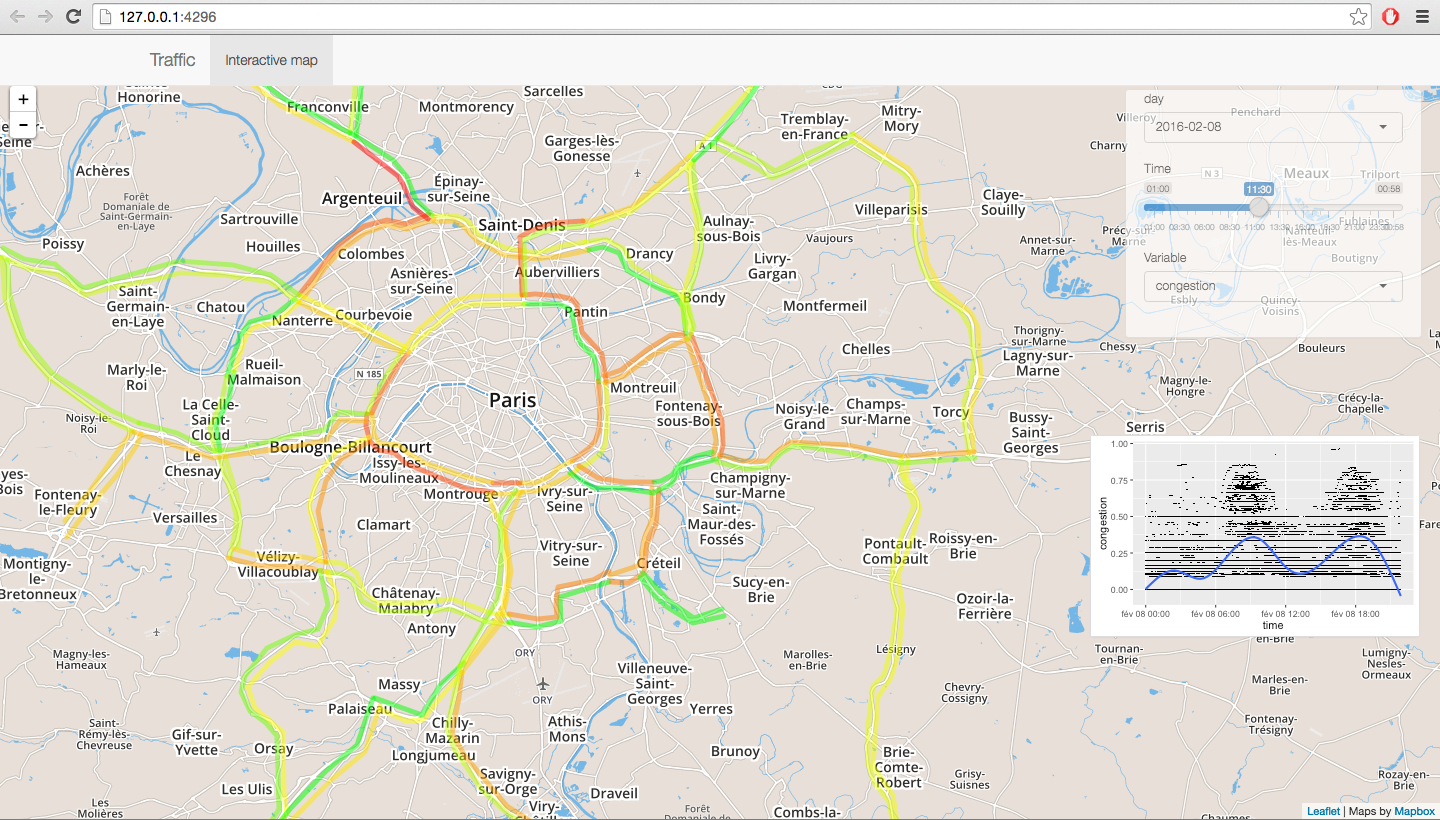
\includegraphics[width=\linewidth]{Figures/TransportationEquilibrium/gr1}
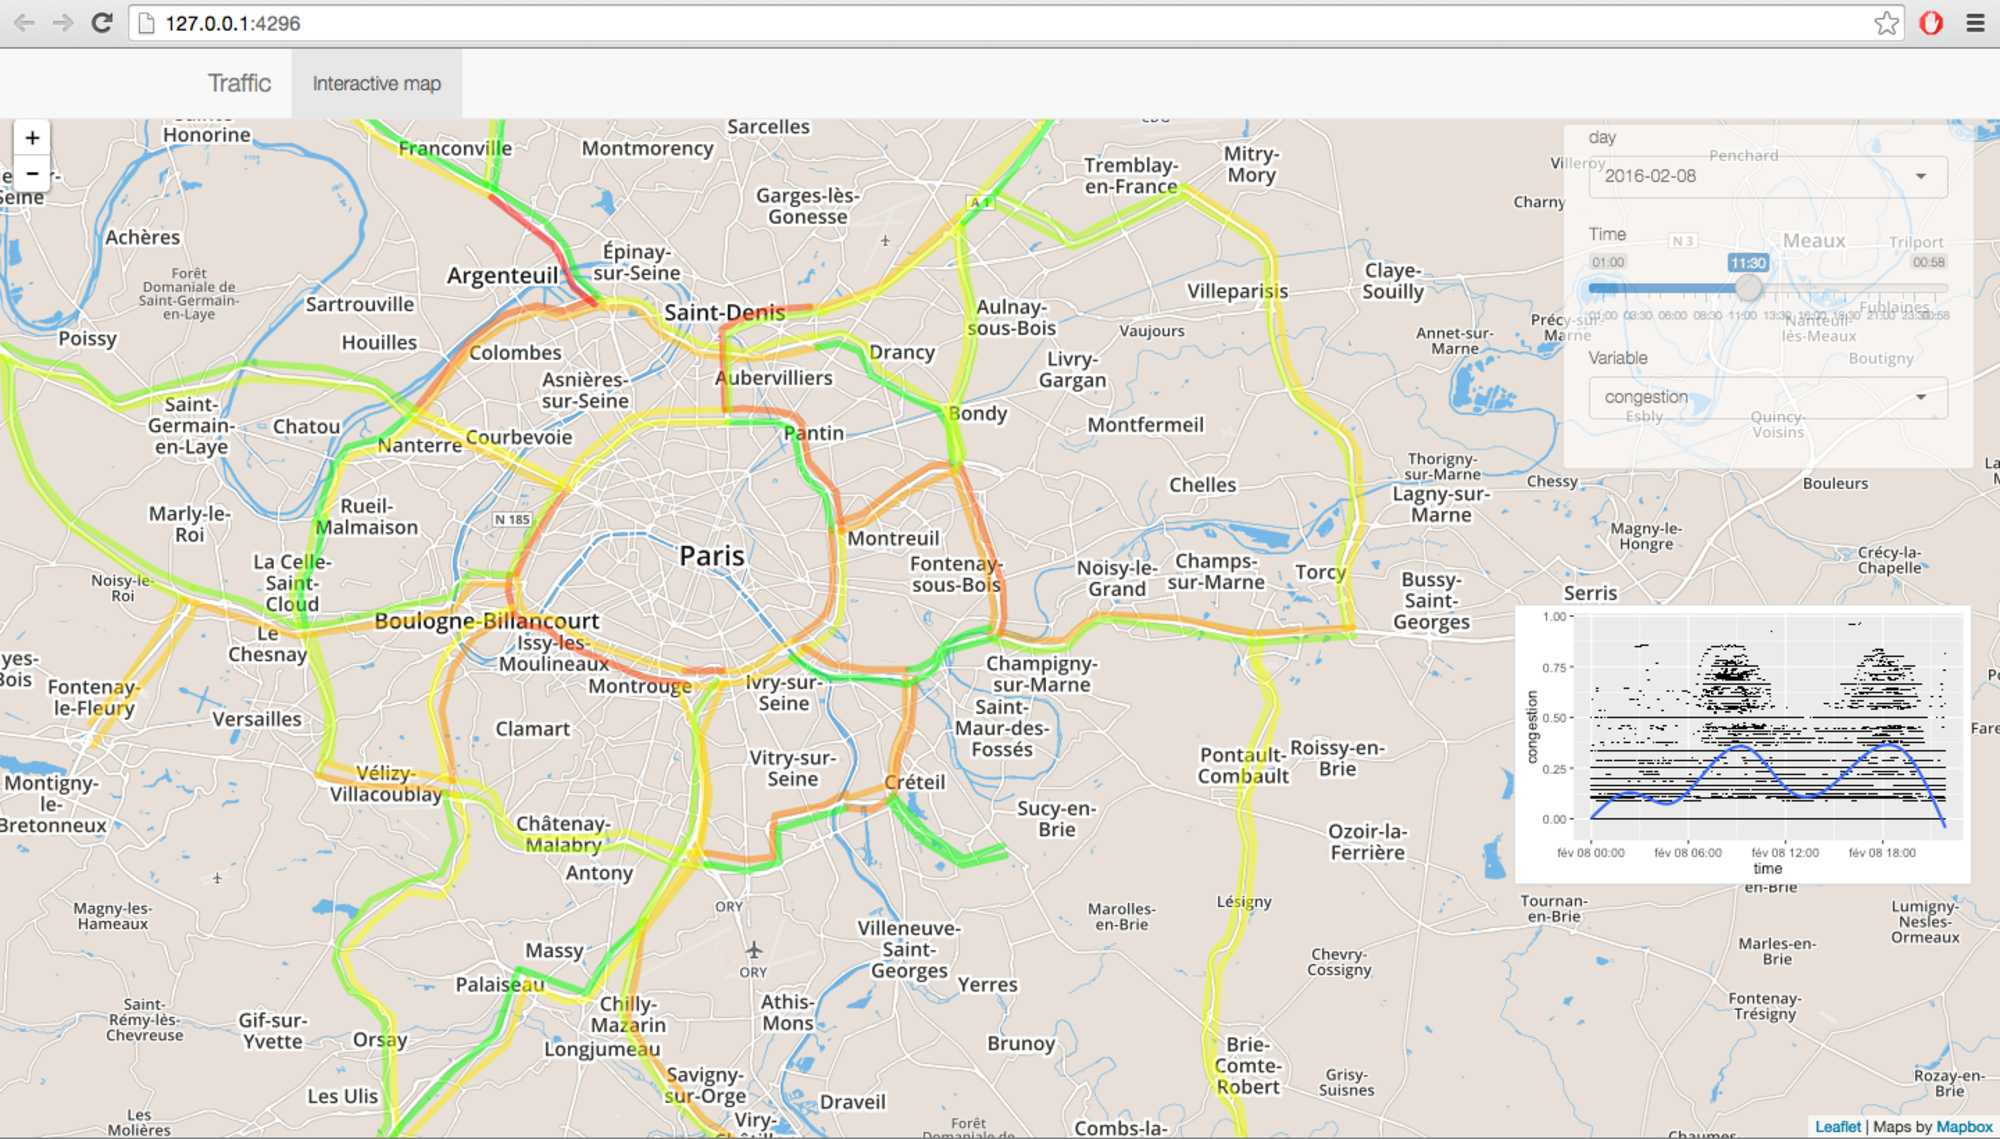
\includegraphics[width=\linewidth]{Figures/Final/8-1-2-fig-transportationequilibrium-fig-1.jpg}
\caption[Web-application for traffic data][Application web pour les données de trafic]{Capture of the web-application to explore spatio-temporal traffic data for Parisian region. It is possible to select date and time (precision of 15min on one month, reduced from initial dataset for performance purposes). A plot summarizes congestion patterns on the current day.\label{fig:transportationequilibrium:fig-1}}{Capture de l'application web\comment[FL]{developpee par/pour (?) qui ?} permettant l'exploration spatio-temporelle des données de traffic pour la région Parisienne. Il est possible de choisir date et heure (précision de 15min sur un mois, réduite par rapport au jeu de données initial pour des raisons de performance). Le graphe en insert résume les motifs de congestion pour la journée courante, en donnant en fonction du temps l'ensemble des valeurs (points noirs) et leur lissage (courbe bleue).\label{fig:transportationequilibrium:fig-1}}
\end{figure}
%%%%%%%%%%%%%%%%%%



%%%%%%%%%%%%%%%%%%%%%%%%
\paragraph{Spatio-temporal Variability of Travel Path}{Variabilité Spatio-temporelle des Trajets}


\bpar{
Following interactive exploration of data, we propose to quantify the spatial variability of congestion patterns to validate or invalidate the intuition that if equilibrium does exist in time, it is strongly dependent on space and localized. The variability in time and space of travel-time shortest paths is a first way to investigate flow stationarities from a game-theoretic point of view. Indeed, the static User Equilibrium is the stationary distribution of flows under which no user can improve its travel time by changing its route. A strong spatial variability of shortest paths at short time scales is thus evidence of non-stationarity, since a similar user will take a few time after a totally different route and not contribute to the same flow as a previous user. Such a variability is indeed observed on a non-negligible number of paths on each day of the dataset. We show in Figure~\ref{fig:fig-2} an example of extreme spatial variation of shortest path for a particular Origin-Destination pair.
}{
A la suite de l'exploration interactive des données, nous proposons de quantifier la variabilité spatiale des motifs de congestion pour valider ou invalider l'intuition que si l'équilibre existe par rapport au temps, il est fortement dépendant de l'espace et localisé. La variabilité spatio-temporelle des plus courts chemins de trajet est une première façon d'étudier la stationnarité des flots d'un point de vue de théorie des jeux. En effet, l'Equilibre Utilisateur Statique est la distribution stationnaire des flots sous laquelle aucun utilisateur ne peut augmenter son temps de trajet en changeant son itinéraire. Une forte variabilité spatiale des plus courts chemins sur de courtes échelles spatiales révèle ainsi une non-stationnarité, puisque un même utilisateur prendra un chemin complètement différent après un court laps de temps et ne contribuera plus au même flot que précédemment. Une telle variabilité est en effet observée sur un nombre non-négligeable de chemins pour chaque jour du jeu de données. La figure~\ref{fig:fig-2} montre un exemple de variation spatiale extrême d'un trajet pour une paire Origine-Destination particulière.
}

\bpar{
The systematic exploration of travel time variability across the whole dataset, and associated travel distance, confirms, as described in Figure 3, that travel time absolute variability has often high values of its maximum across OD pairs, up to 25 minutes with a temporal local mean around 10min. Corresponding spatial variability produces detours up to 35km.
}{
L'exploration systématique de la variabilité du temps de trajet sur l'ensemble du jeu de données, et des distances de trajet associées, confirme, comme présenté en figure~\label{fig:fig-3}, que la variation absolue du temps de trajet présente fréquemment une forte variation de son maximum sur l'ensemble des paires O-D, jusqu'à 25 minutes avec une moyenne temporelle locale autour de 10 minutes. La variabilité spatiale correspondante entraine des détours allant jusqu'à 35km.
}


%%%%%%%%%%%%%%%%%%%
\begin{figure}
%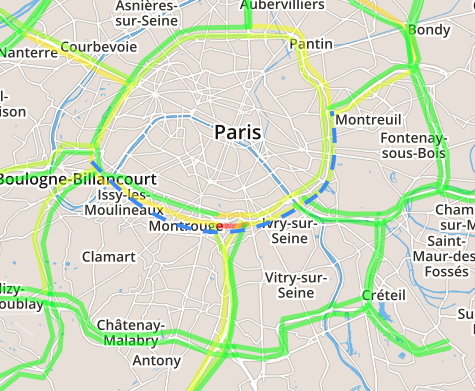
\includegraphics[width=0.47\linewidth]{Figures/TransportationEquilibrium/gr21}
%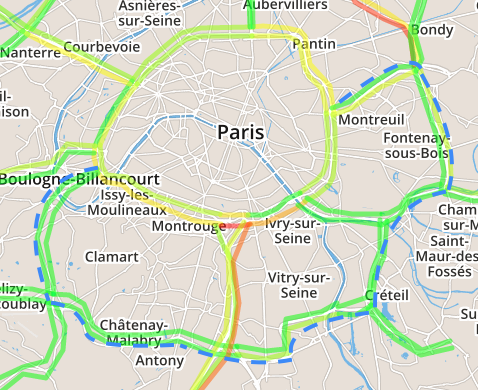
\includegraphics[width=0.47\linewidth]{Figures/TransportationEquilibrium/gr22}
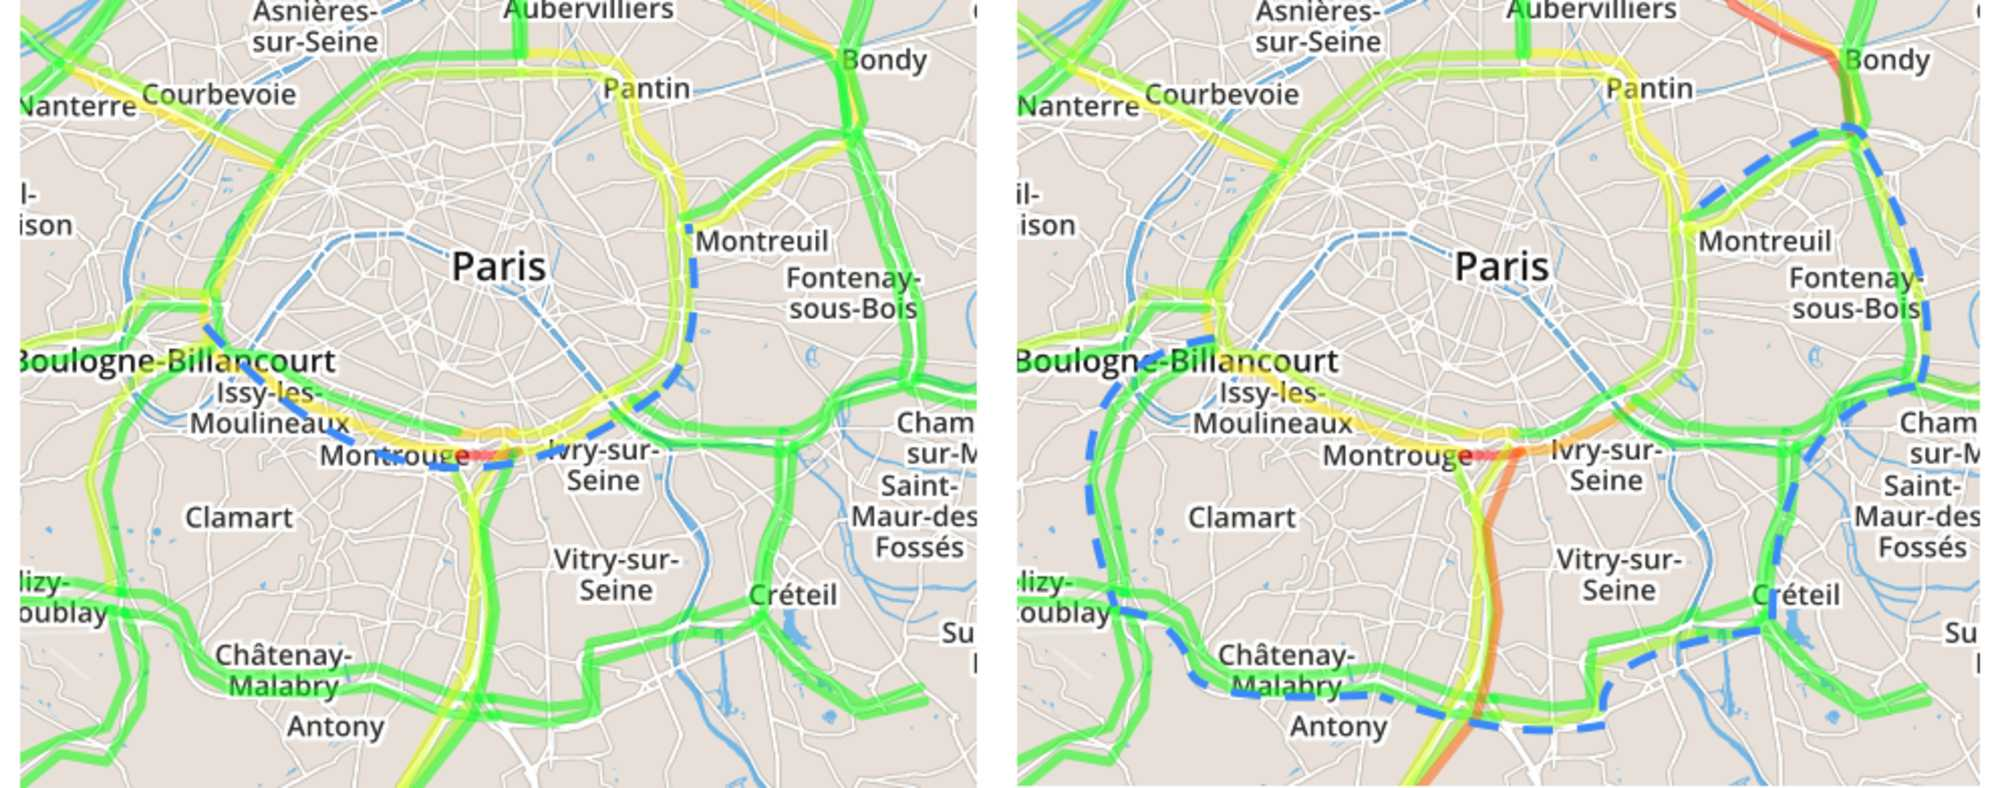
\includegraphics[width=\linewidth]{Figures/Final/8-1-2-fig-transportationequilibrium-fig-2.jpg}
\caption[Spatial variability of shortest paths][Variabilité spatiale des plus courts chemins]{Spatial variability of travel-time shortest path (shortest path trajectory in dotted blue). In an interval of only 10 minutes, between 11/02/2016 00:06 (left) and 11/02/2016 00:16 (right), the shortest path between \emph{Porte d'Auteuil} (West) and \emph{Porte de Bagnolet} (East), increases in effective distance of $\simeq 37$km (with an increase in travel time of only 6min), due to a strong disruption on the ring of Paris.\label{fig:fig-2}}{Variabilité spatiale d'un plus court chemin en temps de trajet (trajet du plus court chemin en pointillé bleu). Dans un intervalle de seulement 10 minutes, entre le 11/02/2016 00:06 (à gauche) et le 11/02/2016 00:16 (à droite), le plus court chemin entre Porte d'Auteuil à l'ouest et Porte de Bagnolet à l'est, augmente en distance effective de $\simeq 37$km (avec une augmentation du temps de trajet de seulement 6 minutes), à cause d'une forte perturbation sur le périphérique parisien.\label{fig:transportationequilibrium:fig-2}}
\end{figure}
%%%%%%%%%%%%%%%%%%%



%%%%%%%%%%%%%%%%%%%
\begin{figure}
%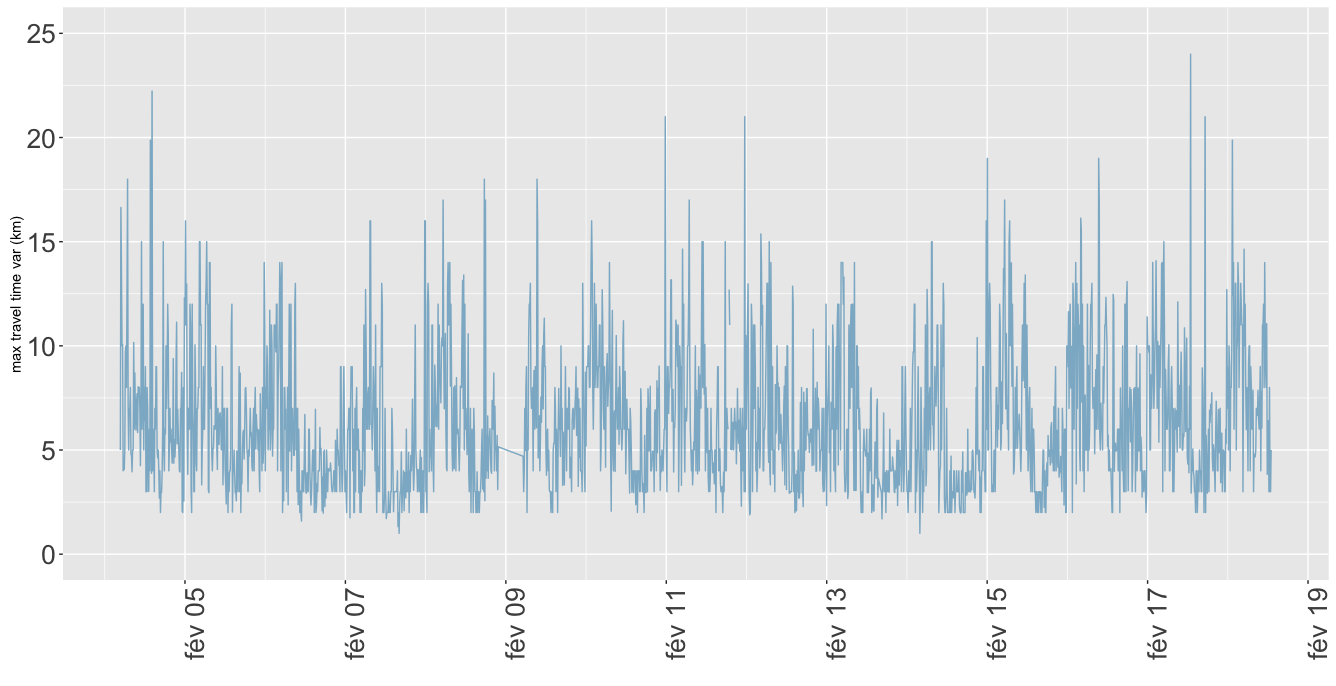
\includegraphics[width=\linewidth]{Figures/TransportationEquilibrium/gr31}
%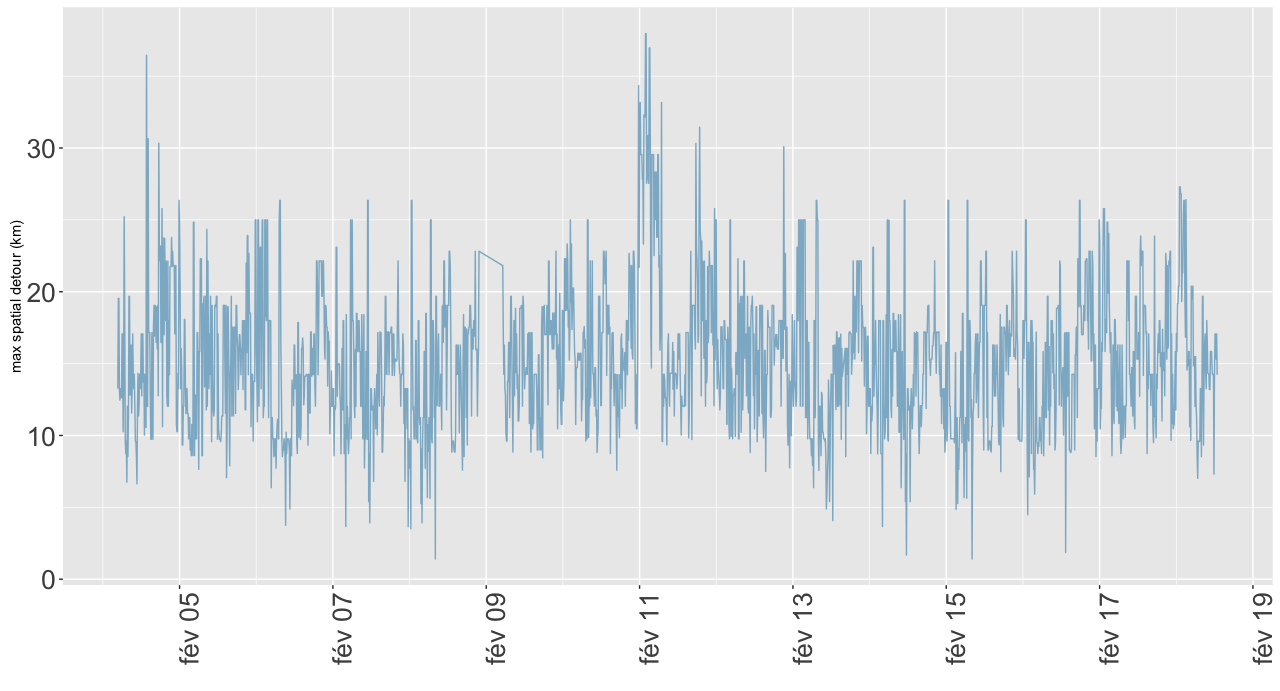
\includegraphics[width=\linewidth]{Figures/TransportationEquilibrium/gr32}
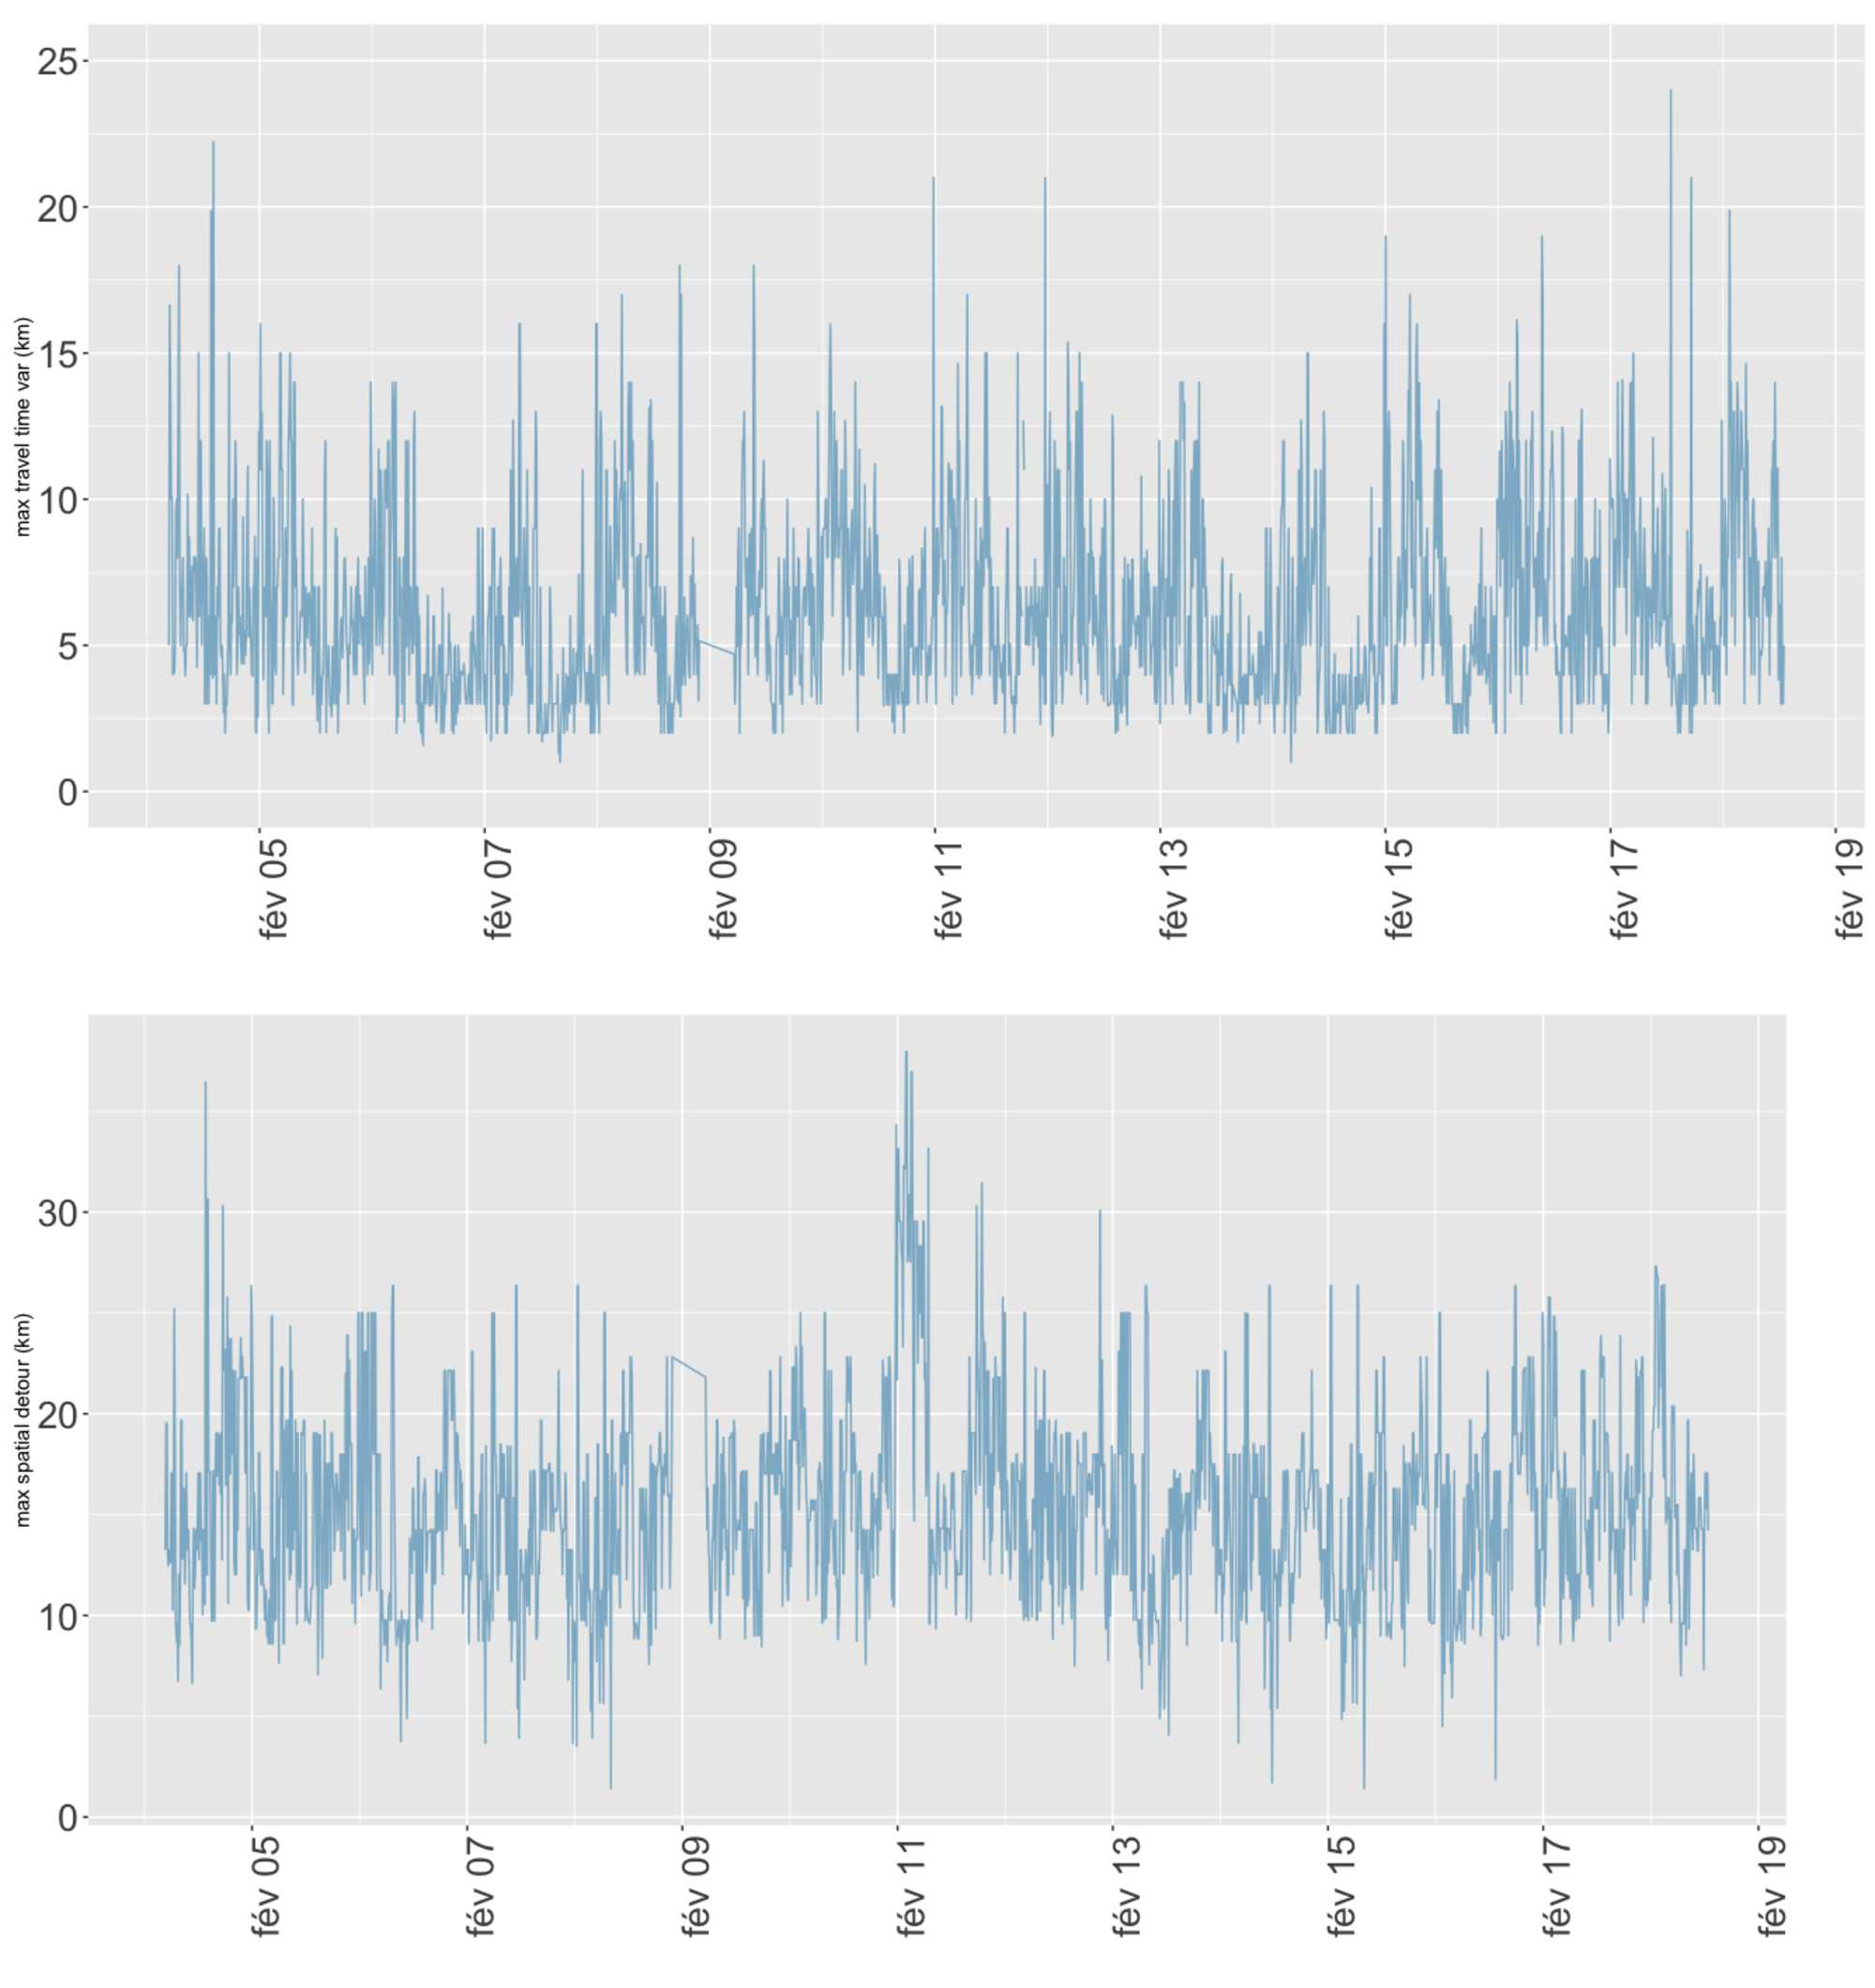
\includegraphics[width=\linewidth]{Figures/Final/8-1-2-fig-transportationequilibrium-fig-3.jpg}
\caption[Variability of travel time and distance][Variabilité des temps de trajet]{Travel time (top) in min and corresponding travel distance (bottom) maximal variability on a two weeks sample. We plot the maximal on all OD pairs of the absolute variability between two consecutive time steps. Peak hours imply a high time travel variability up to 25 minutes and a path length variability up to 35km.\label{fig:transportationequilibrium:fig-3}}{Variabilité maximale du temps de trajet (en haut) en minutes et de la distance de trajet correspondante (en bas) pour un échantillon de deux semaines. Le graphe représente le maximum sur l'ensemble des paires Origine-Destination de la variabilité absolue entre deux pas de temps consécutifs. Les heures de pointe induisent une forte variabilité du temps de trajet, allant jusqu'à 25 minutes et une variabilité de distance jusqu'à 35km.\label{fig:transportationequilibrium:fig-3}\comment[FL]{pourquoi le choix de cet indicateur ? par ex. si le detour correspond a une OD tres tres minoritaire, en quoi est-ce pertinent ?}[(JR) j'avais rajouté cet indicateur pour répondre à une remarque d'un reviewer, mais en effet il casse pas des briques. il faut faire une hypothèse que vu qu'on a une granularité assez grande, la plupart des OD seront réalisés (de plus en prenant les sous-trajets).]}
\end{figure}
%%%%%%%%%%%%%%%%%%%




%%%%%%%%%%%%%%%%%%%
\paragraph{Stability of Network measures}{Stabilité des mesures de réseau}

\bpar{
The variability of potential trajectories observed in the previous section can be confirmed by studying the variability of network properties. In particular, network topological measures capture global patterns of a transportation network. Centrality and node connectivity measures are classical indicators in transportation network description as recalled in~\cite{bavoux2005geographie}. The transportation literature has developed elaborated and operational network measures, such as network robustness measures to identify critical links and measure overall network resilience to disruptions (an example among many is the Network Trip Robustness index introduced in~\cite{sullivan2010identifying}).
}{
La variabilité des trajectoires potentielles observée dans la section précédente peu être confirmée par l'étude de la variabilité des propriétés du réseau. En particulier, les mesures topologiques de réseau capturent les motifs globaux dans un réseau de transport. Les mesures de centralité et de connectivité des noeuds sont des indicateurs classiques pour la description des réseaux de transport comme rappelé par~\cite{bavoux2005geographie}. La littérature en transports a développé des mesures de réseau élaborées et opérationnelles, comme des mesures de robustesse pour identifier les liens critiques et mesurer la résilience globale du réseau aux perturbations (un exemple parmi d'autres est l'indice de \emph{Robustesse du Réseau Effective} introduit dans ~\cite{sullivan2010identifying}).
}



\bpar{
More precisely, we study the betweenness centrality of the transportation network, defined for a node as the number of shortest paths going through the node, i.e. by the equation

%%%%%%%%%%%%%%%
% equation betweeness
\begin{equation}
b_i = \frac{1}{N(N-1)}\cdot \sum_{o\neq d \in V}\mathbbm{1}_{i\in p(o\rightarrow d)}
\end{equation}
%%%%%%%%%%%%%%%

where $V$ is the set of network vertices of size $N$, and $p(o\rightarrow d)$ is the set of nodes on the shortest path between vertices o and d (the shortest path being computed with effective travel times). This index is more relevant to our purpose than other measures of centrality such as closeness centrality that does not include potential congestion as betweenness centrality does.
}{
Plus précisément, nous étudions la centralité de chemin du réseau de transport, défini pour un noeud comme le nombre de plus courts chemins passant par celui-ci, i.e. par l'équation

%%%%%%%%%%%%%%%
% equation betweeness
\begin{equation}
b_i = \frac{1}{N(N-1)}\cdot \sum_{o\neq d \in V}\mathbbm{1}_{i\in p(o\rightarrow d)}
\end{equation}
%%%%%%%%%%%%%%%

où $V$ est l'ensemble des sommets du réseau de taille $N$, et $p(o\rightarrow d)$ est l'ensemble des noeuds sur le plus court chemin entre les sommets $o$ et $d$ (le plus court chemin étant calculé avec le temps de trajet effectif). Cette mesure de centralité est plus adaptée que d'autre dans notre cas, comme la centralité de proximité qui n'inclut pas la congestion potentielle comme la centralité de chemin.
}



\bpar{
We show in Figure 4 the relative absolute variation of maximal betweenness centrality for the same time window than previous empirical indicators. More precisely we plot the value of

%%%%%%%%%%%%%%%
% eq relative variability
\begin{equation}
\Delta b(t) = \frac{\left|\max_i (b_i(t + \Delta t)) - \max_i (b_i(t))\right|}{\max_i (b_i(t))}
\end{equation}
%%%%%%%%%%%%%%%



where $\Delta t$ is the time step of the dataset (the smallest time window on which we can capture variability). This absolute relative variation has a direct meaning : a variation of 20\% (which is attained a significant number of times as shown in Fig.~\ref{fig:fig-4}) means that in case of a negative variation, at least this proportion of potential travels have changed route and the local potential congestion has decrease of the same proportion. In the case of a positive variation, a single node has captured at least 20\% of travels. Under the assumption (that we do not try to verify in this work and assume to be also not verified as shown by~\cite{zhu2010people}, but that we use as a tool to give an idea of the concrete meaning of betweenness variability) that users rationally take the shortest path and assuming that a majority of travels are realized such a variation in centrality imply a similar variation in effective flows, leading to the conclusion that they can not be stationary in time (at least at a scale larger than $\Delta t$) nor in space.
}{
Nous montrons en Fig.~\ref{fig:transportationequilibrium:fig-4} la variation relative absolue du maximum de la centralité de chemin, pour la même fenêtre temporelle que les indicateurs empiriques précédents. Plus précisément, elle est définie par


%%%%%%%%%%%%%%%
% eq relative variability
\begin{equation}
\Delta b(t) = \frac{\left|\max_i (b_i(t + \Delta t)) - \max_i (b_i(t))\right|}{\max_i (b_i(t))}
\end{equation}
%%%%%%%%%%%%%%%


où $\Delta t$ est le pas de temps du jeu de données (la plus petite fenêtre temporelle sur laquelle une variabilité peut être capturée). Cette variation relative absolue a une signification directe : une variation de 20\% (qui est atteinte un nombre significatif de fois comme montré en Figure~\ref{fig:transportationequilibrium:fig-4}) implique dans le cas d'une variation négative, qu'au moins cette proportion de trajectoires potentielles ont changé et que la potentielle congestion locale a décru de la même proportion. Dans le cas d'une variation positive, un seul noeud a capturé au moins 20\% des trajets. Sous l'hypothèse (qu'on ne tente pas de vérifier ici et qu'on peut également supposer non vérifiée comme montré par~\cite{zhu2010people}, mais que l'on utilise comme un outil pour donnée une intuition sur la signification concrète de la variabilité de la centralité) que les utilisateurs choisissent rationnellement le plus court chemin, et supposant que la majorité des trajets est réalisées, une telle variation de la centralité implique une variation similaire dans les flots effectifs, conduisant à la conclusion qu'ils ne peuvent être stationnaires ni dans le temps (au moins sur une échelle plus grande que $\Delta t$) ni dans l'espace.
}




%%%%%%%%%%%%%%%%%%%
\begin{figure}
%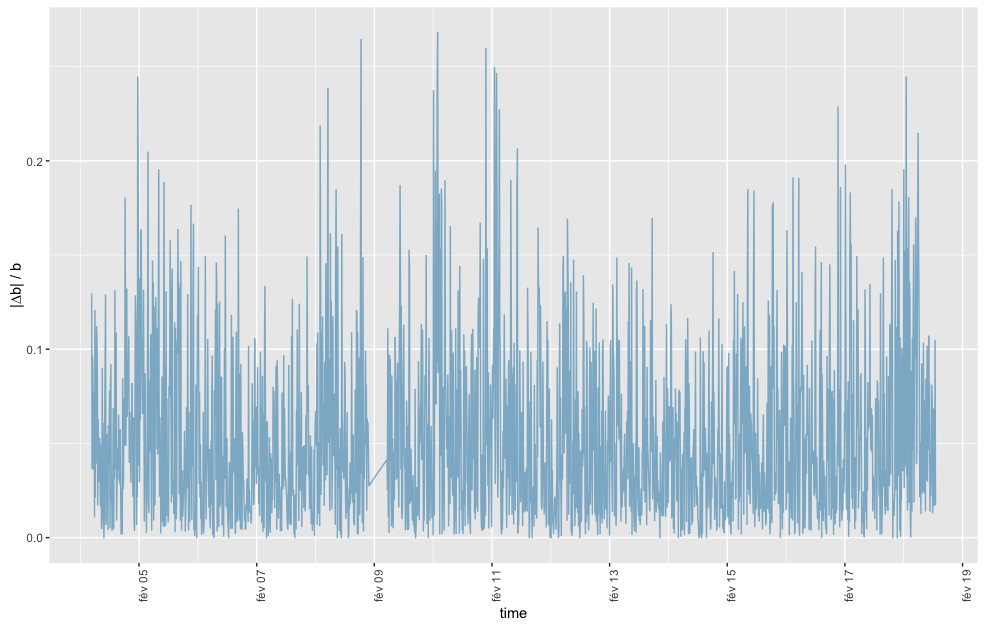
\includegraphics[width=\linewidth]{Figures/TransportationEquilibrium/gr4}
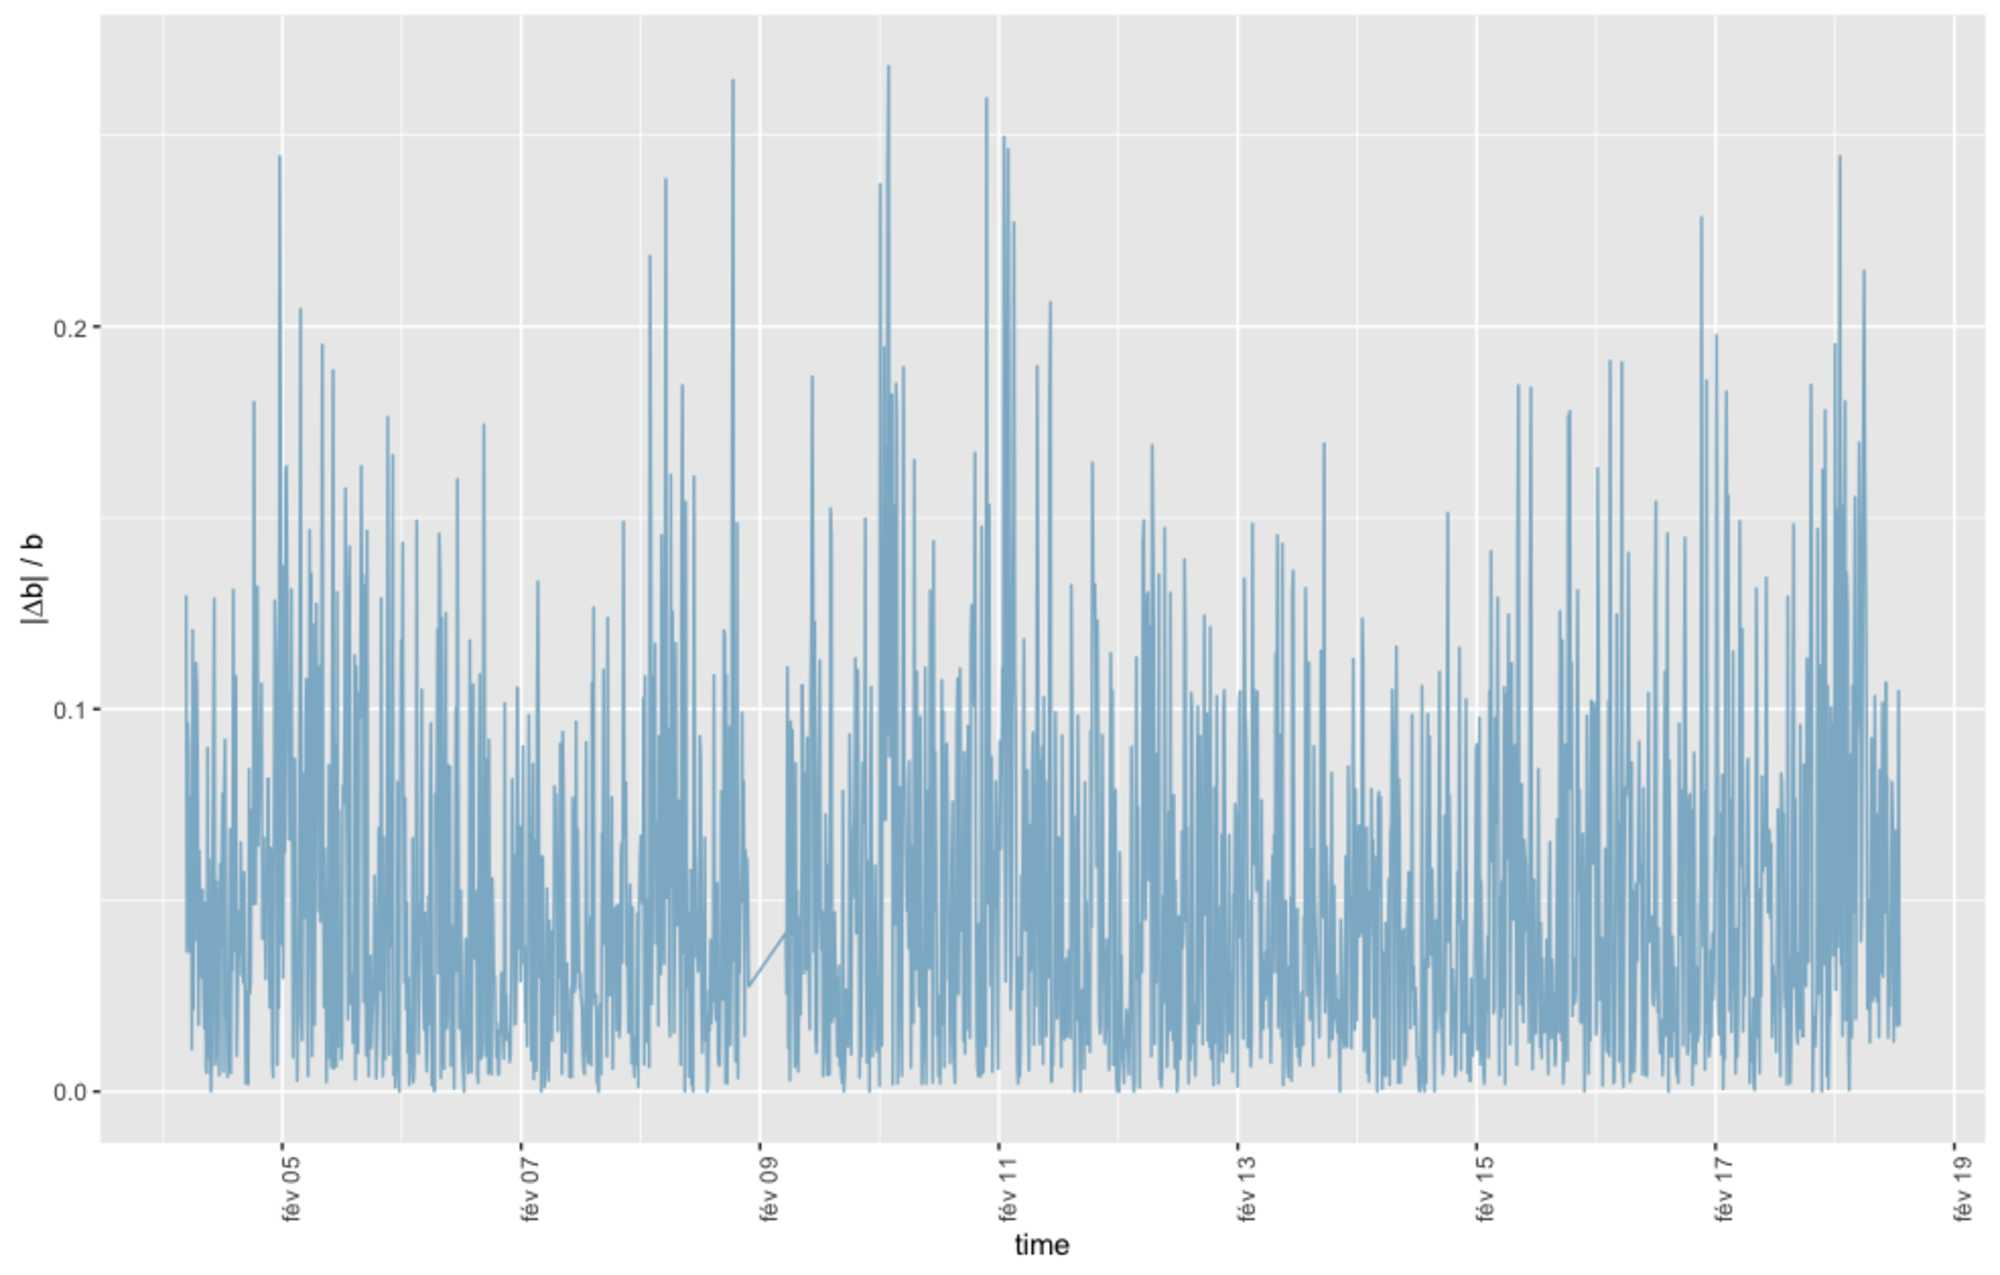
\includegraphics[width=\linewidth]{Figures/Final/8-1-2-fig-transportationequilibrium-fig-4.jpg}
\caption[Temporal stability of maximal betweenness centrality][Stabilité temporelle de la centralité]{Temporal stability of maximal betweenness centrality. We plot in time the normalized derivative of maximal betweenness centrality, that expresses its relative variations at each time step. The maximal value up to 25\% correspond to very strong network disruption on the concerned link, as it means that at least this proportion of travelers assumed to take this link in previous conditions should take a totally different path.\label{fig:transportationequilibrium:fig-4}}{Stabilité temporelle du maximum de la centralité de chemin. Le graphe montre dans le temps la dérivée normalisée du maximum de la centralité de chemin, qui capture ses variations relatives à chaque pas de temps. La valeur maximale de 25\% correspond à de très fortes perturbations du réseau sur les liens correspondants, puisque cela implique qu'au moins cette proportion d'utilisateurs prenant le lien dans des conditions précédentes doivent prendre un trajet complètement différent.\label{fig:transportationequilibrium:fig-4}\comment[FL]{ce n'est pas possible a lire $\rightarrow$ synthetiser}[(JR) pas pertinent de lisser, car c'est justement les max locaux qui nous intéressent.]}
\end{figure}
%%%%%%%%%%%%%%%%%%%





%%%%%%%%%%%%%%%%%%%
\paragraph{Spatial heterogeneity of equilibrium}{Hétérogénéité spatiale de l'équilibre}



\bpar{
To obtain a different insight into spatial variability of congestion patterns, we propose to use an index of spatial autocorrelation, the Moran index (defined e.g. in~\cite{tsai2005quantifying}). More generally used in spatial analysis with diverse applications from the study of urban form to the quantification of segregation, it can be applied to any spatial variable. It allows to establish neighborhood relations and unveils spatial local consistence of an equilibrium if applied on localized traffic variable. At a given point in space, local autocorrelation for variable c is computed by

%%%%%%%%%%%%
% Moran index def
\begin{equation}
\rho_i = \frac{1}{K}\cdot \sum_{i\neq j}{w_{ij}\cdot (c_i - \bar{c})(c_j - \bar{c})}
\end{equation}
%%%%%%%%%%%%

where $K$ is a normalization constant equal to the sum of spatial weights times variable variance and $\bar{c}$ is variable mean. In our case, we take spatial weights of the form $w_{ij} = \exp{\left(\frac{-d_{ij}}{d_0}\right)}$ with $d_0$ typical decay distance and compute the autocorrelation of link congestion localized at link center. We capture therefore spatial correlations within a radius of same order than decay distance around the point $i$. The mean on all points yields spatial autocorrelation index $I$. A stationarity in flows should yield some temporal stability of the index.
}{
Afin d'obtenir un point de vue différent sur la variabilité spatiale des motifs de congestion, nous proposons d'utiliser un indice d'auto-corrélation spatiale, l'indice de Moran (défini par exemple dans~\cite{tsai2005quantifying}). Utilisé plus généralement en analyse spatiale, avec diverses applications allant de l'étude de la forme urbaine à la quantification de la ségrégation, il peut être appliqué à toute variable spatiale. Il permet d'établir des relations de voisinage et révèle la consistence spatiale locale d'un équilibre s'il est appliqué à une variable de traffic localisée. A un point donnée de l'espace, l'auto-corrélation locale pour la variable $c$ est calculée par

%%%%%%%%%%%%
% Moran index def
\begin{equation}
\rho_i = \frac{1}{K}\cdot \sum_{i\neq j}{w_{ij}\cdot (c_i - \bar{c})(c_j - \bar{c})}
\end{equation}
%%%%%%%%%%%%

où $K$ est une constante de normalisation égale à la somme des poids spatiaux fois la variance de la variable et $\bar{c}$ est la moyenne de la variable. Dans notre cas, nous choisissons des poids spatiaux de la forme $w_{ij} = \exp{\left(\frac{-d_{ij}}{d_0}\right)}$ avec $d_0$ distance typique de décroissance. L'auto-corrélation est calculée sur la congestion des liens, localisée au centre du lien. Elle capture ainsi les corrélations spatiales dans un rayon du même ordre que la distance de décroissance autour du point $i$. La moyenne sur l'ensemble des points fournit l'indice d'auto-corrélation spatiale $I$. Une stationnarité des flots devrait impliquer une stabilité temporelle de l'index. 
}



\bpar{
Figure~\ref{fig:transportationequilibrium:fig-5} presents temporal evolution of spatial autocorrelation for congestion. As expected, we have a strong decrease of autocorrelation with distance decay parameter, for both amplitude and temporal average. The high temporal variability implies short time scales for potential stationarity windows. When comparing with congestion (fitted to plot scale for readability) for 1km decay, we observe that high correlations coincide with off-peak hours, whereas peaks involve vanishing correlations. Our interpretation, combined with the observed variability of spatial patterns, is that peak hours correspond to chaotic behaviour of the system, as jams can emerge in any link: correlation thus vanishes as feasible phase space for a chaotic dynamical system is filled by trajectories in an uniform way what is equivalent to apparently independent random relative speeds.
}{
La figure~\ref{fig:transportationequilibrium:fig-5} présente l'évolution temporelle de l'auto-corrélation spatiale pour la congestion. Comme attendu, on observe une forte décroissance de l'auto-corrélation avec la distance de décroissance, à la fois sur l'amplitude et les moyennes temporelles. La forte variabilité temporelle implique de courtes échelles temporelles pour des fenêtres potentielles de stationnarité. Pour une distance de décroissance de 1km, en comparant l'auto-corrélation à la congestion (ajustée à l'échelle du graphe pour lisibilité), on observe que les fortes corrélations coincident avec les heures creuses, tandis que les heures de pointe correspondent à une décroissance des corrélations. Notre interprétation, combinée avec la variabilité observée des motifs spatiaux, est que les heures de pointe correspondent à un comportement chaotique du système, puisque les bouchons peuvent émerger dans n'importe quel lien du réseau : la corrélation disparait alors puisque l'espace des phases atteignables pour un système dynamique chaotique est rempli uniformément par les trajectoires, de façon équivalente à des vitesses relatives qui apparaitraient comme aléatoires et indépendantes.
}



%%%%%%%%%%%%%%%%
\begin{figure}
%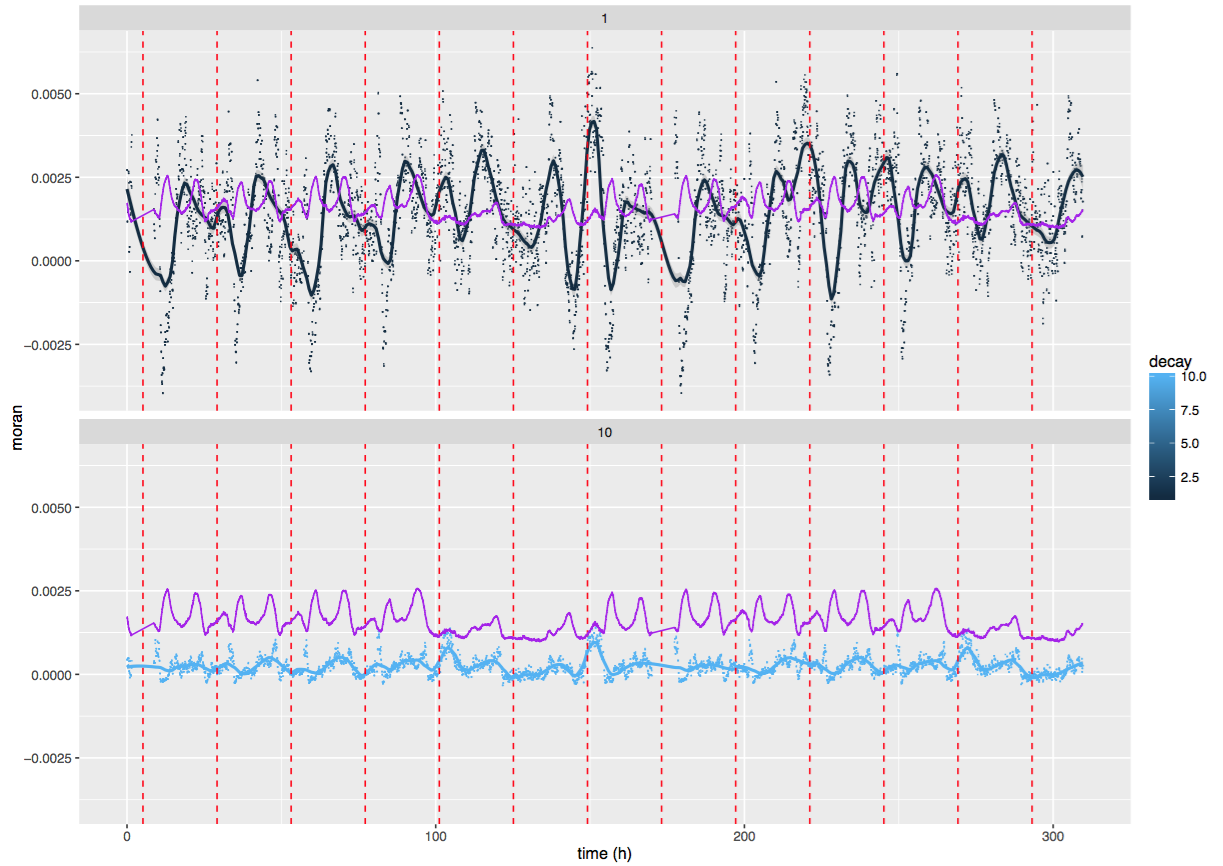
\includegraphics[width=\linewidth]{Figures/TransportationEquilibrium/gr5}
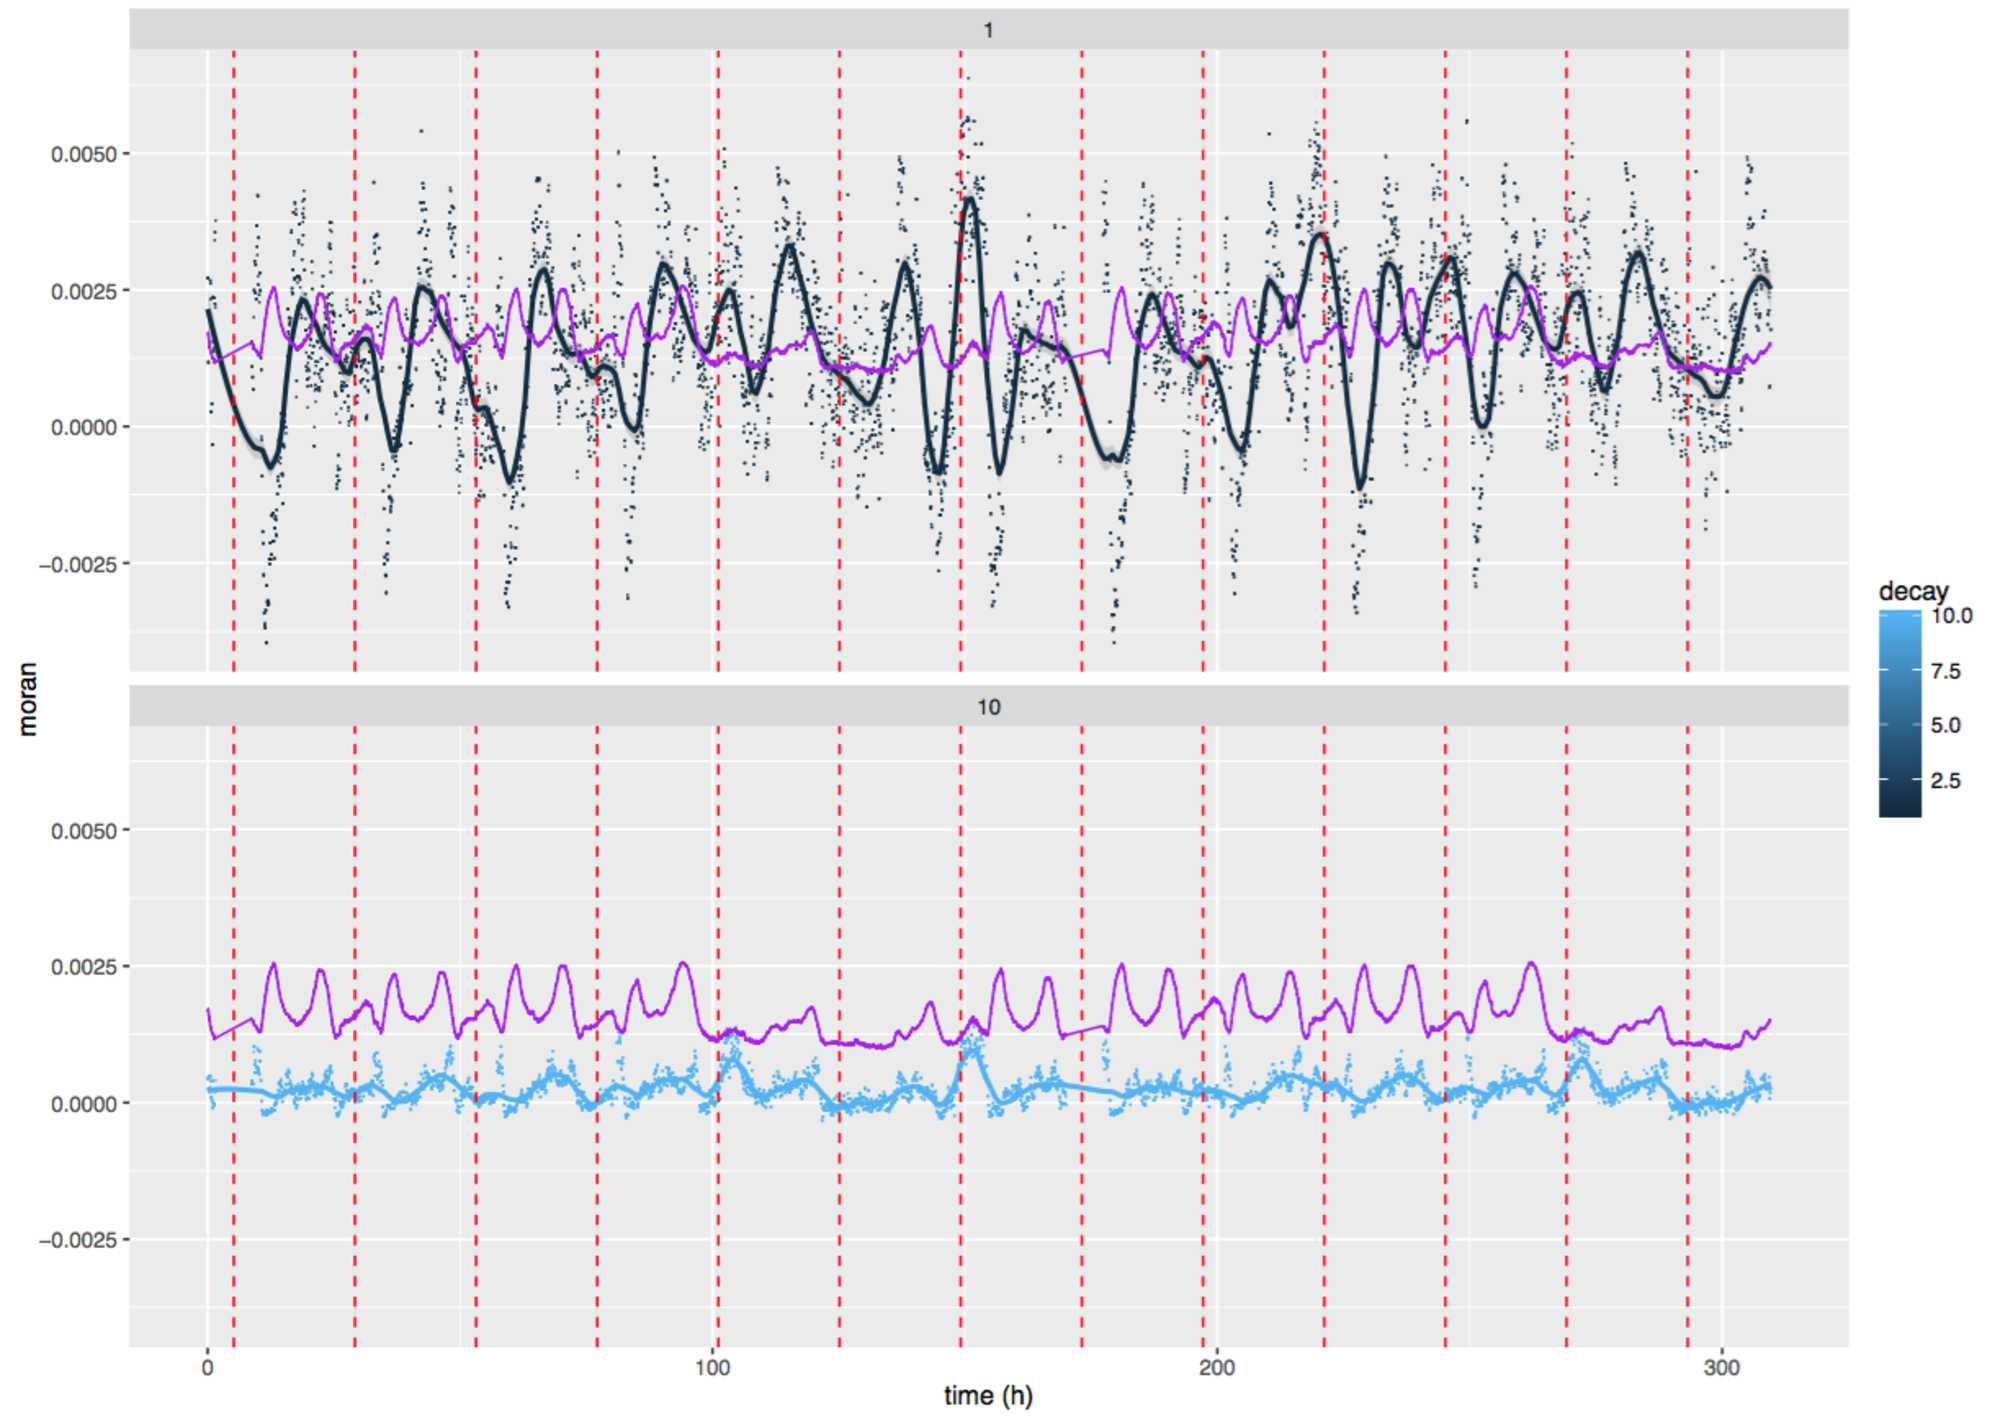
\includegraphics[width=\linewidth]{Figures/Final/8-1-2-fig-transportationequilibrium-fig-5.jpg}
\caption[Spatial auto-correlations for relative travel speed][Auto-corrélation spatiale]{Spatial auto-correlations for relative travel speed on two weeks. We plot for varying value of decay parameter (1,10km) values of auto-correlation index in time. Intermediate values of decay parameter yield a rather continuous deformation between the two curves. Points are smoothed with a 2h span to ease reading. Vertical dotted lines correspond to midnight each day. Purple curve is relative speed fitted at scale to have a correspondence between auto-correlation variations and peak hours.\label{fig:transportationequilibrium:fig-5}}{Auto-corrélations spatiales pour les vitesses relatives sur deux semaines. Le graphe montre les valeurs de l'auto-corrélation dans le temps, pour des valeurs variables (1,10km) de la distance de décroissance. les valeurs intermédiaires de la distance de décroissance donnent une déformation relativement continue entre ces deux extrêmes. Les points sont lissés sur une fenêtre temporelle de 2h pour faciliter la lecture. Les lignes pointillées verticales correspondent à minuit de chaque jour. La courbe violette donne la vitesse relative, ajustée à l'échelle pour établir la correspondance entre les heures de pointe et les variations de l'auto-corrélation.\label{fig:transportationequilibrium:fig-5}}
\end{figure}
%%%%%%%%%%%%%%%%




%%%%%%%%%%%%%%%%%%%%
\subsection{Discussion}{Discussion}

\subsubsection{Theoretical and practical implications of empirical conclusions}{Implications théoriques et pratiques des conclusions empiriques}

\bpar{
We argue that the theoretical implications of our empirical findings do not imply in a total discarding of the Static User Equilibrium framework, but unveil more a need of stronger connections between theoretical literature and empirical studies. If each newly introduced theoretical framework is generally tested on one on more case study, there are no systematic comparisons of each on large and different datasets and on various objectives (prediction of traffic, reproduction of stylized facts, etc.) as systematic reviews are the rule in therapeutic evaluation for example. This imply however broader data and model sharing practices than the current ones. The precise knowledge of application potentialities for a given framework may induce unexpected developments such as its integration into larger models. The example of Land-use and Transportation Interaction studies (LUTI models) is a good illustration of how the SUE can still be used for larger purpose than transportation modeling. \cite{kryvobokov2013comparison} describe two LUTI models, one of which includes two equilibria for four-step transportation model and for land-use evolution (households and firms relocation), the other being more dynamical. The conclusion is that each model has its own advantages regarding the pursued objective, and that the static model can be used for long time policy purposes, whereas the dynamic model provide more precise information at smaller time scale. In the first case, a more complicated transportation module would have been complicated to include, what is an advantage of the static user equilibrium.
}{
Nous formulons l'interprétation que les implications théoriques de ces résultats empiriques n'impliquent pas nécessairement un rejet total du cadre de l'Equilibre Utilisateur Statique, mais révèlent plutôt un besoin de plus fortes connexions entre la littérature théorique et les études empiriques. Si chaque nouveau cadre théorique introduit est généralement testé sur un cas ou plus, il n'existe pas de comparaisons systématiques de chacun sur des jeux de données de grande taille et variés, et pour des objectifs d'application différents (prédiction du traffic, reproduction de faits stylisés, etc.), à l'image des revues systématiques qui sont la règle en évaluation thérapeutique par exemple.\comment[FL]{source ?} Cela implique cependant des pratiques de partage des données et des modèles plus larges que celles existant couramment. La connaissance précise des potentialités d'application d'un cadre donné peut induire des développements inattendus comme l'intégration dans des modèles plus larges. L'exemple des études des interaction entre Transport et Usage du Sol (modèles \emph{LUTI}) est une bonne illustration d'un cas ou le EUS peut toujours être utilisé avec des motivations plus larges que la modélisation du traffic. \cite{kryvobokov2013comparison} décrit deux modèles \emph{LUTI}, dont l'un inclut deux équilibres pour les modèles de transport à quatre temps et pour l'évolution de l'usage du sol (localisation des ménages et emplois), l'autre étant dynamique. La conclusion est que chaque modèle à ses avantages au regard de l'objectif poursuivi, et que le modèle statique peut être utilisé pour comparer des politiques sur le temps long, tandis que le modèle dynamique fournit de l'information plus précise à de plus petites échelles temporelles. Dans le premier cas, un module de transport plus compliqué aurait été plus difficile à inclure, ce qui est un avantage du EUS dans ce cas.
}


\bpar{
Concerning practical applications, it seems natural that static models should not be used for traffic forecast and management at small time scales (week or day) and efforts should be made to implement more realistic models. However the use of models by the planning and engineering community is not necessarily directly related to academic concerns and state-of-the-art. For the particular case of France and mobility models, \cite{commenges2013invention} showed that engineers had gone to the point of constructing inexistent problems and implementing corresponding models that they had imported from a totally different geographical context (planning in the United States). The use of one framework or type of model has historical reasons that may be difficult to overcome.
}{
Concernant les applications pratiques, il semble naturel\comment[FL]{je ne pense pas que tu as prouve cela : tu ne dis pas comment sont utilises ces modeles} que les modèles statiques ne devraient pas être utilisés pour la prédiction et la gestion du traffic sur de petites échelles temporelles (semaine ou jour) et que des efforts doivent être faits pour implémenter des modèles plus réalistes. Cependant, l'utilisation des modèles par la communautés des ingénieurs et des planificateurs n'est pas directement reliée aux enjeux académiques et à l'état de l'art dans le domaine. Dans le cas particulier de la France et des modèles de mobilité, \cite{commenges2013invention} a montré que les ingénieurs allaient jusqu'au point de construire des problèmes inexistants et d'implémenter les modèles correspondants qu'ils avaient importé d'un contexte géographique totalement différent (la planification aux Etats-Unis). L'utilisation d'un cadre ou d'un type de modèle a des raisons historiques qui peuvent être difficiles à surmonter.

}


\subsubsection{Towards explanative interpretations of non-stationarity}{Vers des interprétations de la non-stationnarité}


\bpar{
An assumption we formulate regarding the origin of non-stationarity of network flows, in view of data exploration and quantitative analysis of the database, is that the network is at least half of the time highly congested and in a critical state. The off-peak hours are the larger potential time windows of spatial and temporal stationarity, but consist in less than half of the time. As already interpreted through the behavior of autocorrelation indicator, a chaotic behavior may be at the origin of such variability in the congested hours. The same way a supercritical fluid may condense under the smallest external perturbation, the state of the link may qualitatively change with a small incident, producing a network disruption that may propagate and even amplify. The direct effect of traffic events (notified incidents or accidents) can not be studied without external data, and it could be interesting to enrich the database in that direction. It would allow establishing the proportion of disruptions that do appear to have a direct effect and quantify a level of criticality of network congestion in time, or to investigate more precise effects such as the consequences of an incident on traffic of the opposite lane.
}{
Une hypothèse qu'on peut formuler concernant l'origine de la non-stationnarité des flots dans le réseau, au regard de l'exploration des données et des analyses quantitatives, est que le réseau est au moins la moitié du temps fortement congestionné et dans un état critique. Les heures creuses sont les plus grandes fenêtres temporelles potentielles de stationnarité spatiale et temporelle, mais couvre moins de la moitié du temps. Comme déjà interprété dans le comportement de l'indicateur d'auto-corrélation, un comportement chaotique pourrait être à l'origine d'une telle variabilité lors des heures congestionnées. A la manière d'un fluide supercritique qui condense sous une perturbation externe infinitésimale, l'état d'un lien peut qualitativement changer par un petit incident, produisant une perturbation du réseau qui se propage et peut même s'amplifier. L'effet direct des évènements du traffic (incidents signalés ou accidents) ne peut pas être étudié sans source de données extérieure, et un enrichissement de la base de données dans cette direction pourrait être intéressante. Cela permettrait d'établir la proportion de perturbations qui paraissent avoir un effet direct et quantifier un niveau de caractère critique de la congestion du réseau dans le temps, ou d'étudier plus précisément des phénomènes localisés comme les conséquences d'un incident de traffic sur la voie opposée.
}



\subsubsection{Possible developments}{Développements}


\bpar{
Further work may be planned towards a more refined assessment of temporal stability on a region of the network, i.e. the quantitative investigation of consideration of peak stationarity given above. To do so we propose to compute numerically Liapounov stability of the dynamical system ruling traffic flows using numerical algorithms such as described by~\cite{goldhirsch1987stability}. The value of Liapounov exponents provides the time scale by which the unstable system runs out of equilibrium. Its comparison with peak duration and average travel time, across different spatial regions and scales should provide more information on the possible validity of the local stationarity assumption. This technique has already been introduced at an other scale in transportation studies, as e.g.~\cite{tordeux2016jam} that study the stability of speed regulation models at the microscopic scale to avoid traffic jams.
}{
Le travail futur pourra être planifié dans la direction d'une étude de la stabilité temporelle sur des zones du réseau, i.e. l'étude quantitative précise de la non-stationnarité des heures de pointes découverte ci-dessus. Pour cela nous proposons de calculer numériquement la stabilité de Liapounov du système dynamique régissant les flots de traffic, par l'intermédiaire d'algorithmes numériques comme ceux décrits par~\cite{goldhirsch1987stability}. La valeur des exposants de Liapounov fournit l'échelle de temps sur laquelle le système instable s'éloigne de l'équilibre. Leur comparaison avec la durée des heures de pointe et le temps de trajet moyen, sur différentes zones spatiales et différentes échelles, devrait fournir plus d'information sur une possible validité de l'hypothèse de stationnarité locale. Cette technique a déjà été introduite à une autre échelle dans les études de transport, comme e.g.~\cite{tordeux2016jam} qui étudie la stabilité des modèles de régulation de vitesse à l'échelle microscopique pour éviter l'émergence de congestion.
}


\bpar{
Other research directions may consist in the test of other assumptions of static user equilibrium (as the rational shortest path choice, which would be however difficult to test on such an aggregated dataset, implying the use of simulation models calibrated and cross-validated on the dataset to compare assumptions, without necessarily a direct clear validation or invalidation of the assumption), or the empirical computation of parameters in stochastic or dynamical user equilibrium frameworks. 
}{
D'autres directions de recherche peuvent consister en le test des autres hypothèses du EUS (comme le choix rationnel du plus court chemin, qui serait cependant difficile à tester à un tel niveau d'agrégation, impliquant l'utilisation de modèles de simulation calibrés et cross-validés sur le jeu de données pour comparer différentes hypothèses, sans toutefois nécessairement une validation ou invalidation directe de l'hypothèse), ou le calcul empirique des paramètres dans les cadres d'Equilibre Utilisateur Stochastique ou Dynamique.
}



\subsubsection{Conclusion}{Conclusion}


\bpar{
We have described an empirical study aimed at a simple but from our point of view necessary investigation of the existence of the static user equilibrium, more precisely of its stationarity in space and time on a metropolitan highway network. We constructed by data collection a traffic congestion dataset for the highway network of Greater Paris on 3 months with two minutes temporal granularity. The interactive exploration of the dataset with a web application allowing spatio-temporal data visualization helped to guide quantitative studies. Spatio-temporal variability of shortest paths and of network topology, in particular betweenness centrality, revealed that stationarity assumptions do not hold in general, what was confirmed by the study of spatial autocorrelation of network congestion. We suggest that our findings highlight a general need of higher connections between theoretical and empirical studies, as our work can discard misunderstandings on the theoretical static user equilibrium framework and guide the choice of potential applications.
}{
Nous avons décrit une étude empirique ayant pour but une étude simple, mais selon notre point de vue nécéssaire, de l'existence de l'équilibre utilisateur statique, plus précisément de sa stationnarité dans le temps et l'espace pour un réseau routier métropolitain principal. Un jeu de données de congestion du trafic est construite par collection de données, pour le réseau du Grand Paris sur 3 mois avec une granularité temporelle de 2 minutes. L'exploration interactive du jeu de données via une application web permettant la visualisation spatio-temporelle aide à guider les analyses quantitatives. La variabilité spatio-temporelle des plus courts chemins et de la topologie du réseau, en particulier la centralité de chemin, révèle que l'hypothèse de stationnarité ne tient généralement pas, ce qui est confirmé par l'étude de l'auto-corrélation spatiale de la congestion du réseau. Nous suggérons que nos résultats soulignent un besoin général de plus grandes connexions entre les études théoriques et empiriques, puisque cette étude permet de chasser les incompréhensions théoriques sur l'Equilibre Utilisateur Statique, et guider le choix d'application potentielles.
}



\stars








%%%%%%%%%%%%%%%
% Stylized facts : empirical analysis



% Chapter 

\chapter{Empirical Analysis : Insights from Stylized Facts} % Chapter title

\label{ch:empirical} % For referencing the chapter elsewhere, use \autoref{ch:name} 

%----------------------------------------------------------------------------------------


\headercit{Mais ce n'est pas une question d'{\^a}ge, de chiffres et de stats\\ Moi je te parle surtout de rage, de kif et d'espoir}{Youssoupha}{\textit{, Esperance de Vie}}


\bigskip


%  plan : 

%  1) static morphological analysis : requires a formal link between temporal and spatial correlations ?  -- typology etc can already be interesting --


%  2) presentation of BP case study

%  3) base Bien

%  4) Work with Solène



%----------------------------------------------------------------------------------------


As this quote suggests, a purely quantitative view of the world makes no sense without qualitative counterbalancing. More precisely, we argue that the \textit{clich{\'e}} of an opposition between quantitative and qualitative analysis is an illusion. No distinct boundary exists between both. We propose to call quantitative any process involving computation by a Turing machine, whereas the qualitative will be for us the modeling design process and its interpretations. Therefore both are necessarily closely interlaced in any of our approaches. In particular concerning the construction and the validation or refutation of our theory, empirical analysis on real case studies, implying the extraction and qualification of stylized facts, follows that schema.

% articulation with theoretical questions
% articulation with modeling

We propose in this chapter various empirical analysis on different objects at different scales. A first section begins the examination of static spatial correlations between morphological measures of population density and road network measures on Europe at a 500m resolution. Applying last section of the methodological chapter should provide information on typical spatial scales of interaction between these indicators of territory and network and on dynamical correlations between these. These computation furthermore provide empirical measures on which one model will be calibrated. We then describe a roadmap for statistical analysis on dynamical data of interactions for Bassin Parisien in the last fifty years. An other project using Real Estate transaction data for Parisian Metropolitan Region aim at seeking early warning of network breakdowns. We finally describe potential analyses on South African historical data.



%----------------------------------------------------------------------------------------


%%%%%%%%
%  Section : static analysis
%%%%%%%%

\newpage

\section{Static correlations of urban form and network shape}{Corrélations Statiques entre Forme Urbaine et Forme de Réseau}


Spatio-temporal processes implying diffusion or propagation phenomena generally have a specific structure of correlation. In particular, as derived in section~\ref{sec:spatiotempcorrs}, a static computation of correlation between different instances of a system may under certain conditions provide information on dynamical correlations implied.


% justify scale studied here


%%%%%%%%%%%%%%%%%%
\subsection{Morphological Measures of European Population Density}{Mesures morphologiques de la densité de population européenne}

\subsubsection{Context}{Contexte}


\bpar{
At the macroscopic scale of system of cities, spatialization of the urban system is reasonably captured by cities position, associated with aggregated city variable to represent entirely the system (see e.g. ontologies of Simpop models~\cite{pumain2012multi} or its successor Marius~\cite{cottineau2014evolution}). At the mesoscopic scale at which we aim to capture morphological manifestations of interactions between transportation networks and territories, structure of the territorial system can be specified by more refined indicators for the morphological aspect.
% TODO biblio spatial structure etc Florent
}{
A l'échelle macroscopique du système de ville, le caractère spatial du système urbain est capturé de manière raisonnable par les positions des villes, associées aux variables agrégées au niveau de la ville qui représentent entièrement le système (voir e.g. l'ontologie des modèles Simpop~\cite{pumain2012multi} ou de leur successeur Marius~\cite{cottineau2014evolution}). A l'échelle mesoscopique, à laquelle nous nous attendons à capturer des manifestations morphologiques des interactions entre ville et transport, la structure du système territorial peut être spécifiée par des indicateurs plus raffinés pour l'aspect morphologique.
}


\subsubsection{Empirical Analysis}{Analyse Empirique}

We study systematically morphological indicators for constant size areas covering European Community. The choice of fixed size areas can be questioned regarding definition of a territorial system, that can be otherwise understood as a consistent spatial entity at a given scale and along certain criteria : \emph{Human territories} as defined by Raffestin (op. cit.) or more generally functionally autonomous spaces\footnote{for example, a tentative of definition of a \textit{Parisian} territory would present many facets. From the subjective territory point of view, intra-muros Parisians consider a strict boundary at \textit{Boulevard Periph{\'e}rique}, whereas close and even further suburbs will be seen as Parisians from the Province. The functional territory of \textit{Metropolitain} extends slightly further than the administrative boundary. Governance perimeters are currently mutating with the Metropolitan governance project. Complementary perceptions of the territory can thus be multiplied.}. Here we choose the mesoscopic scale of a metropolitan center ($\simeq$ 50km) for comparability purposes and because greater scale are no more relevant regarding urban form, whereas smaller scales must contain too much noise. 

Data is the European population density grid~\cite{eurostat} and indicators computation is implemented in parallel using \texttt{R} with Fast convolution raster functions. We show in next figures computed values of morphological indicators (see \cite{le2015forme} for a precise formulation of indicators that are Moran index, average distance, entropy and hierarchy).



%%%%%%%%%%%%%%%%%%
\begin{figure}
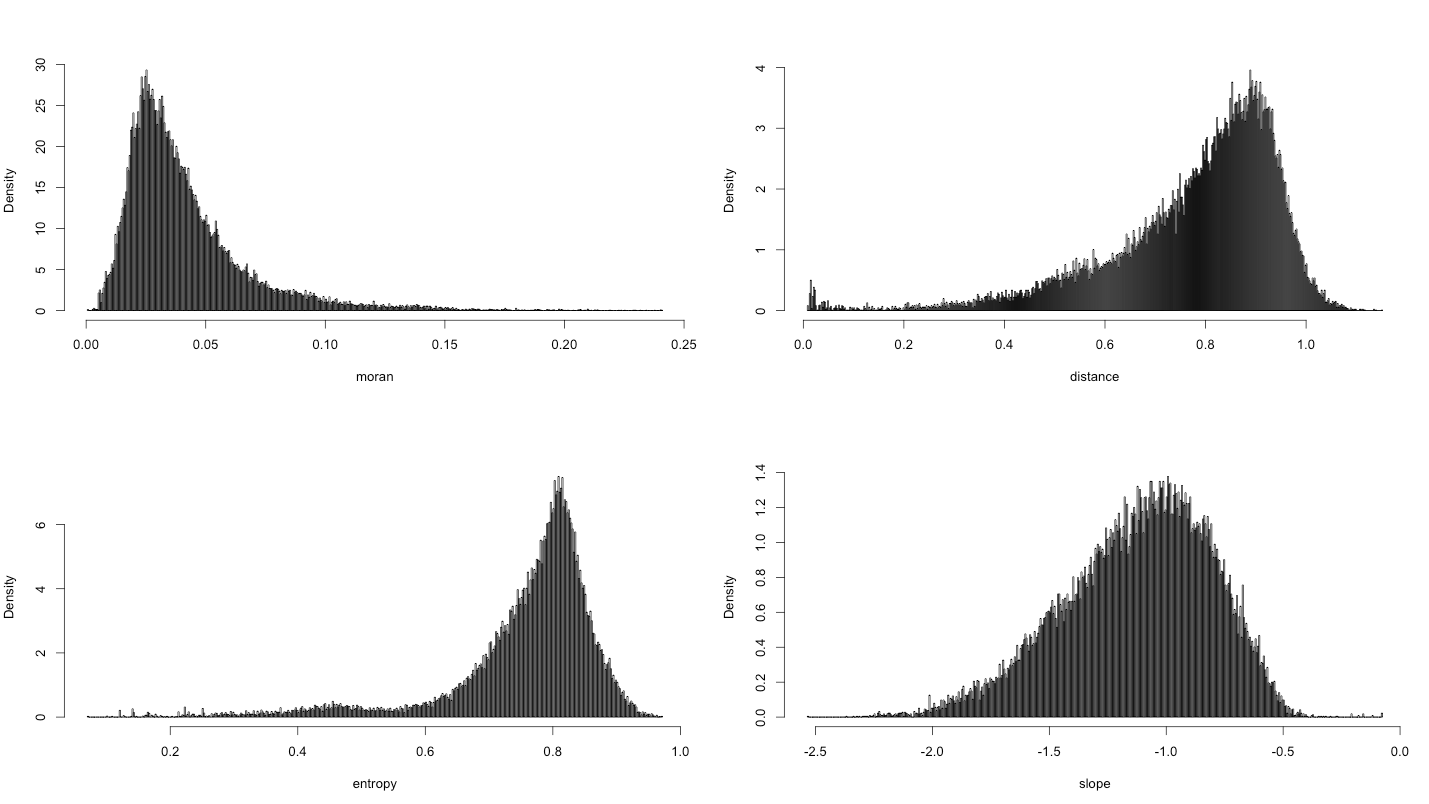
\includegraphics[width=1.2\textwidth]{Figures/PartII/Empirical/Static/Density/hists_GOOD}
\caption[Empirical Distribution of Morphological Indicators]{Empirical Distribution of Morphological Indicators}{Distribution empirique des indicateurs morphologiques}
\end{figure}
%%%%%%%%%%%%%%%%%%

%%%%%%%%%%%%%%%%%%
\begin{figure}
\hspace{-5cm}
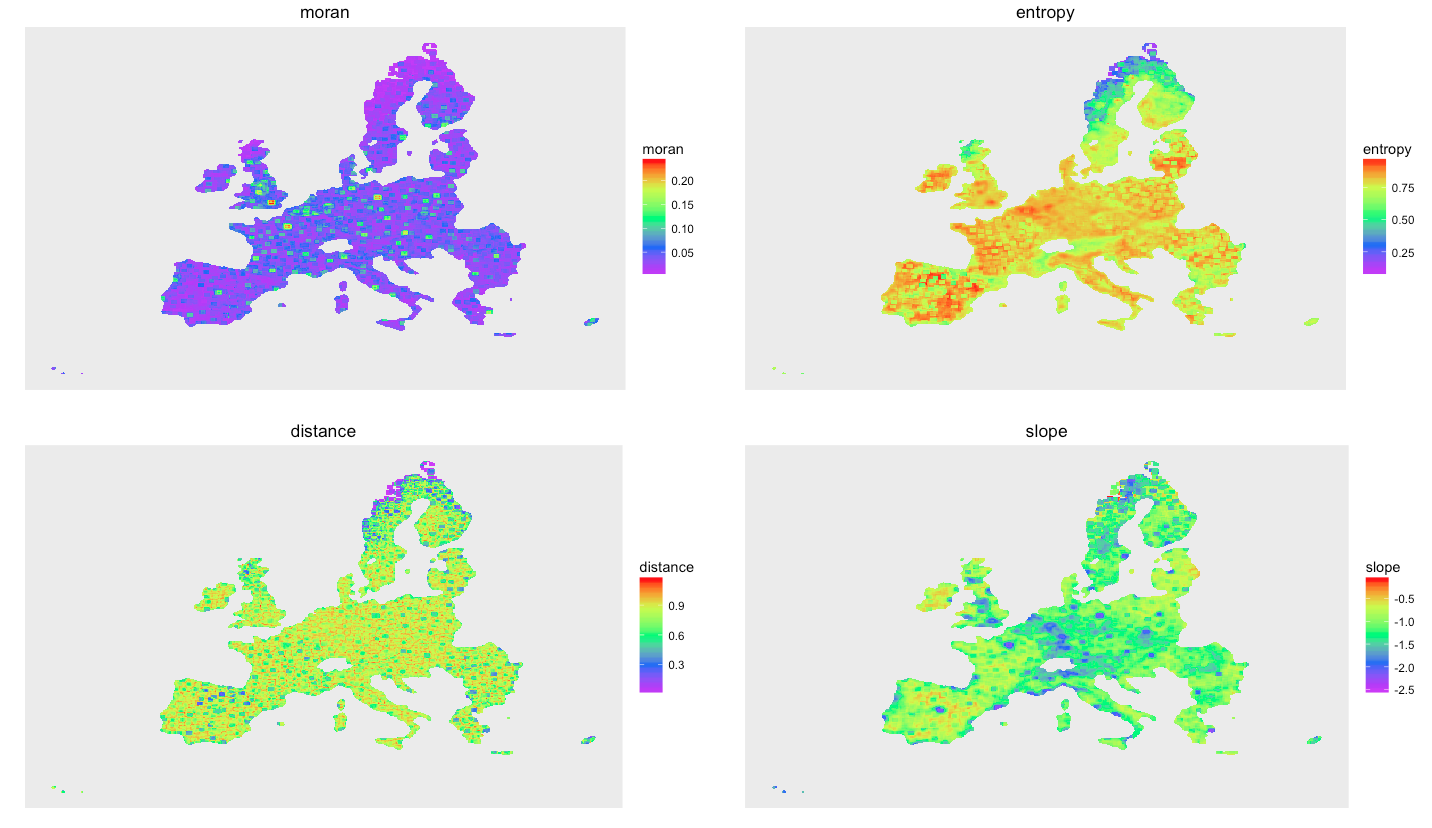
\includegraphics[angle=90,width=1.7\textwidth,height=\textheight]{Figures/PartII/Empirical/Static/Density/all_50km}
\caption[Geographical Distribution of Morphologies]{Geographical Distribution of Morphologies : value of indicators across Europe.}{}
\end{figure}
%%%%%%%%%%%%%%%%%%


%%%%%%%%%%%%%%%%%%
\begin{figure}
\hspace{-3cm}
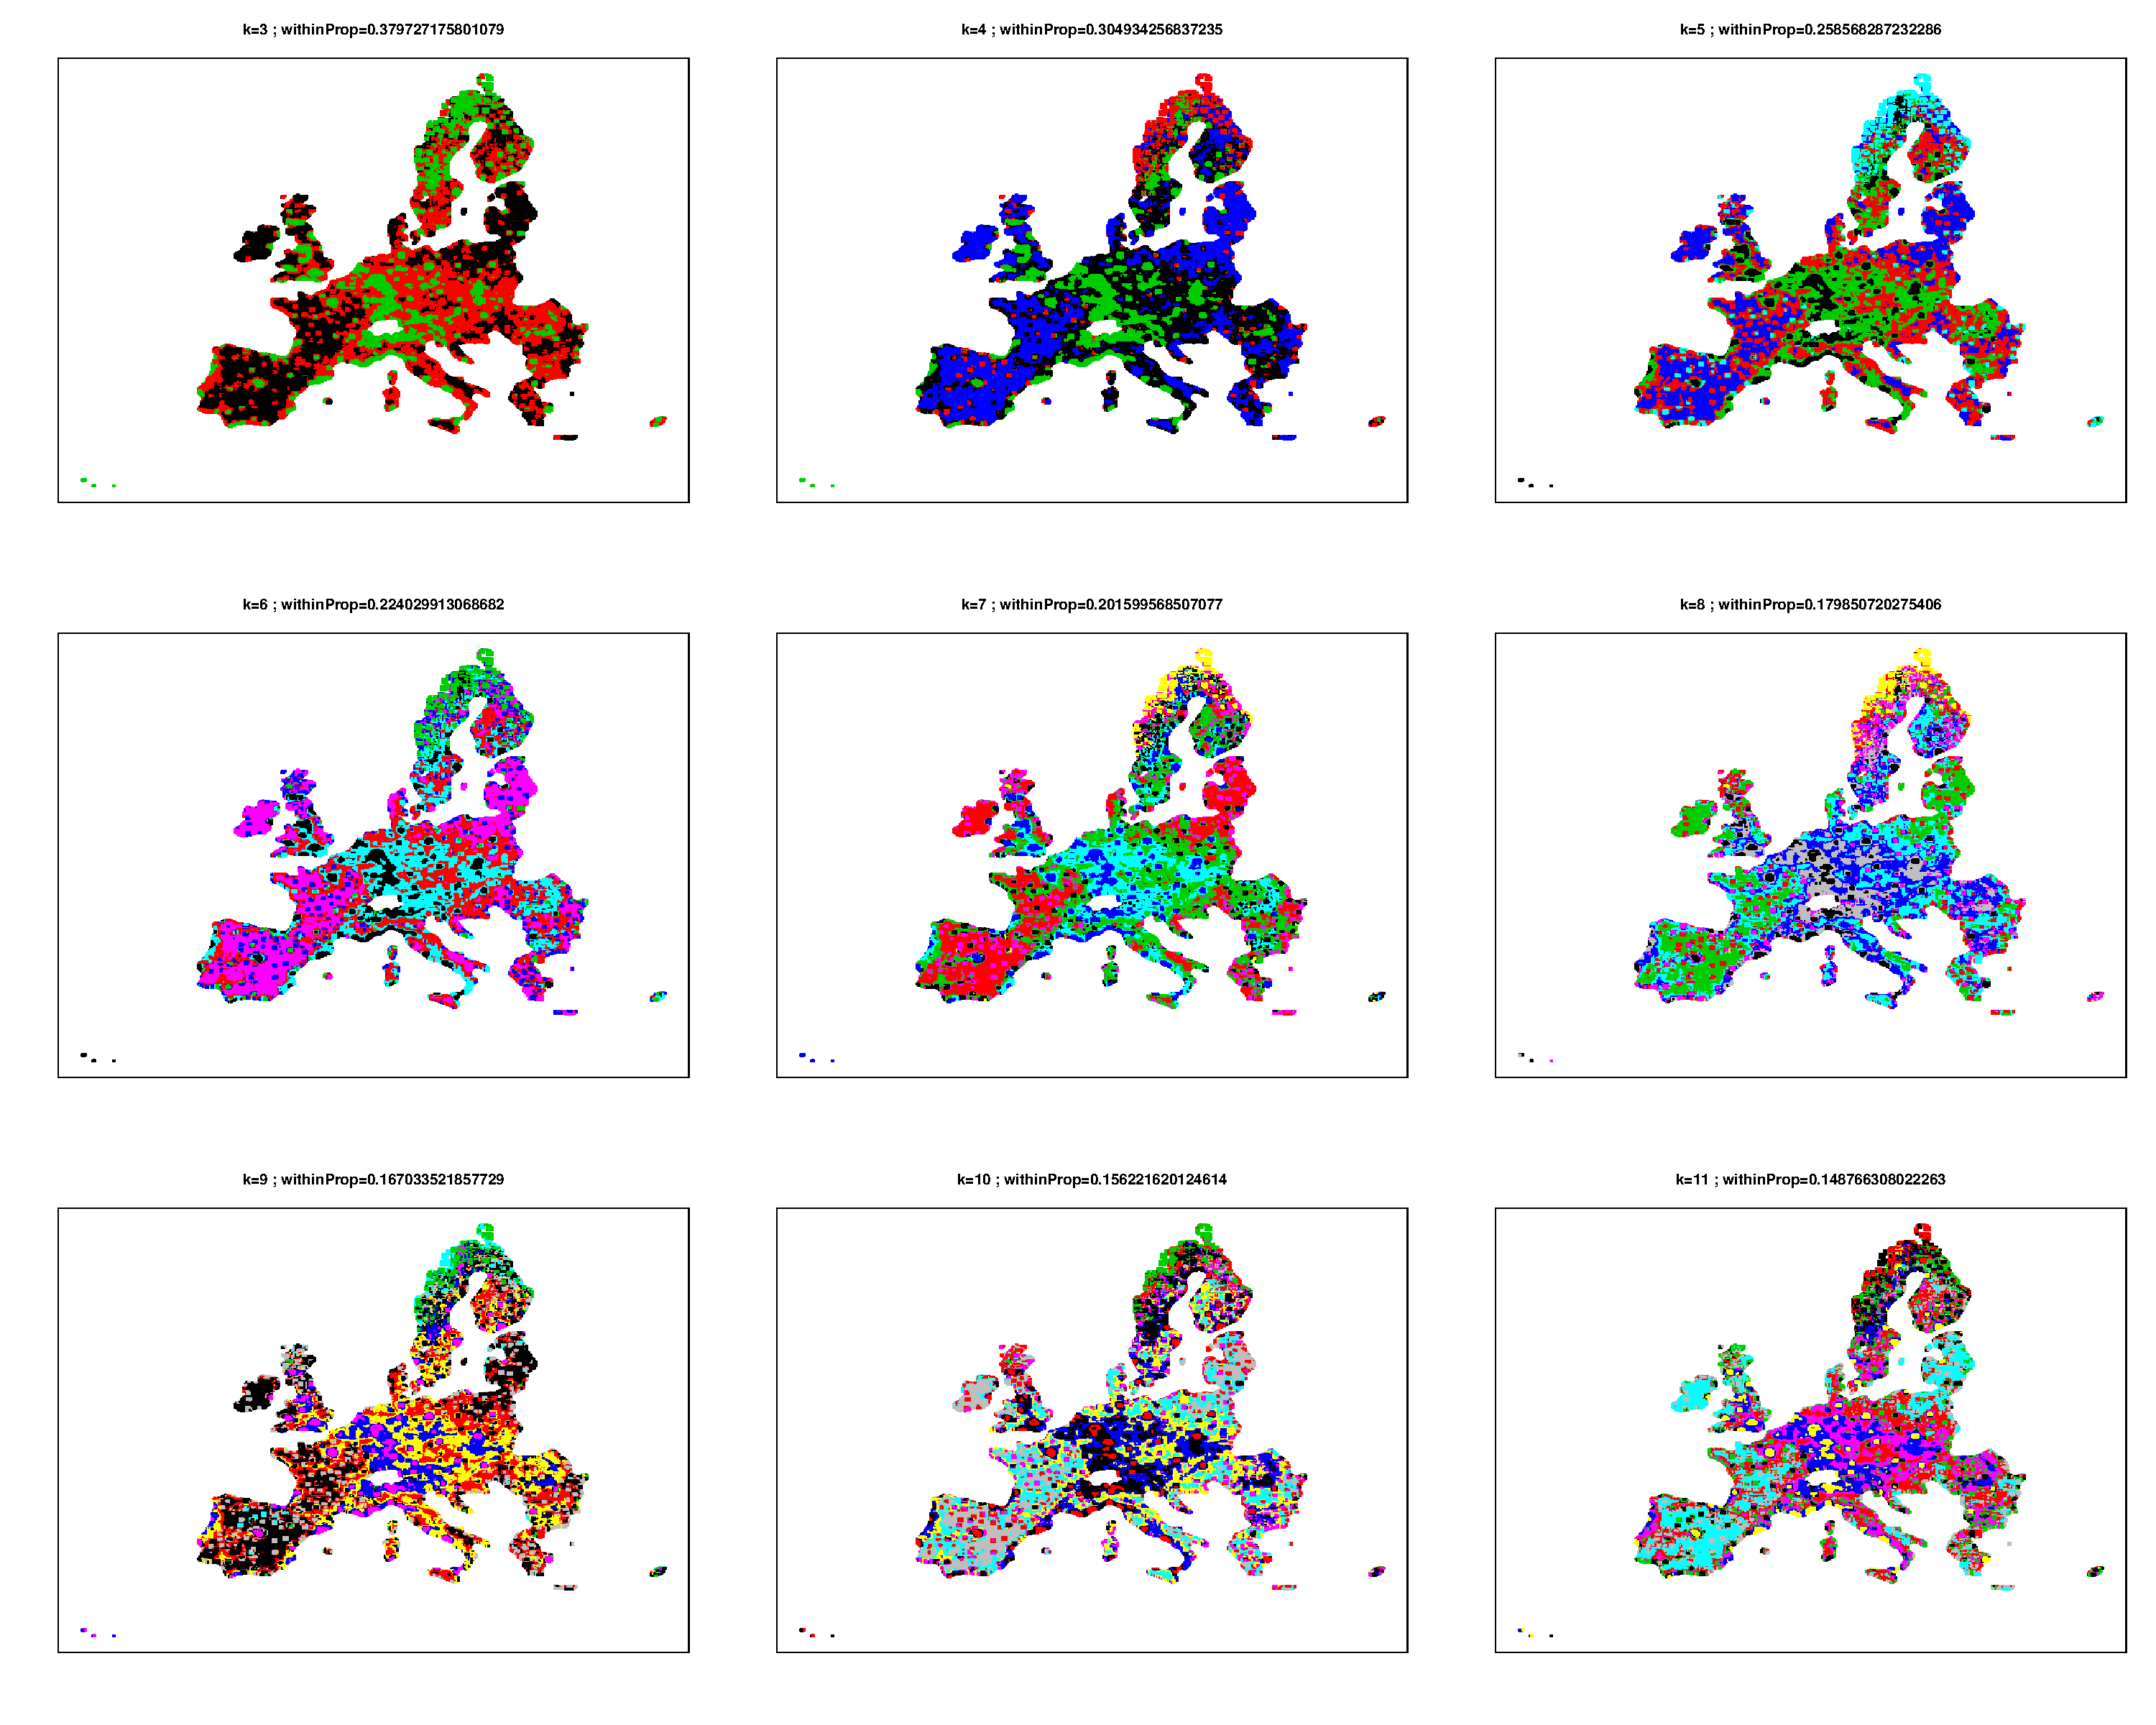
\includegraphics[angle=90,width=1.7\textwidth,height=\textheight]{Figures/PartII/Empirical/Static/Density/clust_k3-11}
\caption[Clustering Analysis of Morphologies]{Clustering Analysis of Morphologies. We present the results of an average k-means for different values of }{}
\end{figure}
%%%%%%%%%%%%%%%%%%






\subsubsection{Further developments}{Développements}

In \cite{10.1371/journal.pone.0107042} density grids for other countries across the world (ex. China) are provided\footnote{available at \url{http://www.worldpop.org.uk/}} soo we may repeat our analysis to other regions for comparison purposes.



%%%%%%%%%%%%%%%%%%
\subsection{Network Measures}{Mesures de Réseau}

We consider network aggregated indicators as a way to characterize transportation network properties on a given territory, the same way morphological indicators yielded information on urban structure. We propose to compute some simple indicators on same extents as for morphology, to be able to explore relations between these static measures. Static network analysis has been extensively documented in the literature, see \cite{louf2014typology} for a cross-sectional study of cities or \cite{2015arXiv151201268L} for exploration of new measures for the road network.


\subsubsection{Data preprocessing}{Pré-traitement des données}

We work in a first time on road network, which structure is finely conditioned to territorial configuration of population densities. Furthermore, data for present day road network is available through the OpenStreetMap project~\cite{openstreetmap}. Its quality was investigated for different countries such as England~\cite{haklay2010good} and France~\cite{girres2010quality}. It was found to be of a quality equivalent to official surveys for the primary road network.

% data collected from http://download.geofabrik.de/europe.html

% TODO : remarque : why not include artwork as appendix. science<->art (// poésies ?)



\paragraph{Simplification algorithm}{Algorithme de simplification}

For a given dataset corresponding to a subset of the overall road network, it is necessary to simplify network structure by spatial aggregation as initial data presents very detailed features and thus a very large numbers of nodes ($\simeq 10^10$ for Europe dataset). Such a level of precision is not needed in our study since density data is already aggregated at 500m resolution. It is possible to drastically reduce network size by spatial aggregation of nodes and link replacements. More precisely we use the following procedure :
\begin{itemize}
\item a background raster (which resolution $r$ gives the snapping parameter for aggregation) is constructed from a reference raster and the extent of network. This grid gives spatial aggregation units for network nodes.
\item for each feature of the road dataset, corresponding connected raster cells are stored with corresponding impedance and distance in a sparse adjacency matrix.
\item Network is simplified by iterative suppression of nodes with degree two, with keeping link speed and real length to their effective value.
\end{itemize}


\paragraph{Implementation}{Implémentation}

A \texttt{PostGIS} database is used to store raw and simplified network, in order to perform efficient spatial requests, compared for example to initial \texttt{osm} data formats (\texttt{osm} or \texttt{pbf}). However the size of storage of data into this base is much higher (factor 10) so processing was parallelized between european countries. Consistence is ensured by the use of the same common density raster as simplification canvas. Final network is stored into the Postgis database for efficient indicator computation given a spatial extent.


\paragraph{Sensitivity to simplification parameters}{Sensibilité aux paramètres de simplification}

Sensitivity of indicators to raster resolution and to degree simplification algorithm must still be tested to ensure the relevance of data preprocessing.


\subsubsection{Indicators}{Indicateurs}

Network macroscopic structure is summarized by the following set of indicators, after the simplifications and reductions done in the previous step. Assuming network given by $N=(V,E)$, nodes spatial positions $\vec{x}(V)$ and edges \emph{effective distances} $d(E)$ taking into account impedances and real distances (to include basically network hierarchy), we have indicators :
\begin{itemize}
\item connectivity
\item degree distribution
\item centrality, taken as normalized mean \emph{betweenness-centrality}
\item average path length
\item network diameter
\item mean network speed
\end{itemize}

These indicators are used to capture a rough picture of the structure. Refined work at smaller scales (intra-urban road network) and with more elaborated measures that allow to differentiate more precisely local form, was recently done by Lagesse in~\cite{2015arXiv151201268L}.



\subsubsection{Results}{Résultats}


\bpar{}{
Les indicateurs de réseau ont été calculés sur des zones similaires aux indicateurs de forme urbaine, 

}






%%%%%%%%%%%%%%%%%%
\subsection{Effective static correlations}{Correlations Statiques Effectives}







%%%%%%%%%%%%%%%%%%
\subsection{Spatial non-stationarity and non-ergodicity}{Non-stationnarité spatiale et non-ergodicité}



Case study : Context and Rationale
% interactions between networks and territories

\textbf{Study of interactions between network and territories :}

\medskip

$\rightarrow$ \textit{searching for stylized facts, what can be learnt from static correlations between urban form and road network ?}

\bigskip

\textbf{Theoretical Background : } \textit{A Theory of co-evolutive networked human territories} proposed in~\cite{raimbault2016memoire}, that in particular postulates an important role of networks in the morphogenesis of complex adaptive urban systems that are human territories

\bigskip

$\rightarrow$ \textit{investigation of stationarity and ergodicity properties of relation between road network and population distribution ; implies spatiality of correlations and link static-dynamic}
% because means link between dynamic and static ; and also spatiality of correlations




Dataset construction
% brief description of nw simplification ; 

Computation of topological road network for all Europe, at 100m granularity scale (to be used consistently with population grid~\cite{eurostat})

\medskip

$\rightarrow$ Import of OSM into \texttt{pgsql}, simplification at 100m granularity, topological simplification with split/merge algorithm

\bigskip
%
%\begin{columns}
%\begin{column}{width=0.7\textwidth}
%
%\end{column}
%\begin{column}{width=0.3\textwidth}
%\textit{.} % TODO summary stats here.
%\end{column}
%\end{columns}

%\begin{columns}
%\begin{column}{0.7\textwidth}
    %\includegraphics[width=\textwidth,height=0.5\textheight]{figures/ex_nw}
%\end{column}
%\begin{column}{0.3\textwidth}
   \textit{$\simeq 44\cdot 10^6$ links in initial OSM db, $\simeq 61\cdot 10^6$ in first simplified layer, $\simeq 21\cdot 10^6$ in final database}
%\end{column}
%\end{columns}







%%%%%%%%%%%%%%%%%
Results : Computation of Indicators


\textit{Computation of urban form indicators~\cite{le2015forme} and network indicators on $l_0=10km$ side square}

%\includegraphics[width=\textwidth]{figures/pop-alphaBetweenness}




%%%%%%%%%%%%%%%%%
Results : Spatial Correlations

\textit{Computation of spatial correlation on square areas of width $\delta\cdot l_0$ (with typically $\delta = 4, \ldots , 16$)}

\centering

%\includegraphics[width=\textwidth,height=0.7\textheight]{figures/corr_PCA_delta4}

$\rightarrow$ \textit{local spatial stationarity of processes}



%%%%%%%%%%%%%%%%%
%\sframe{Results : Stationarity scales}{
% maps
% 
%}



%%%%%%%%%%%%%%%%%
Results : Multi-scale Processes
% plots
%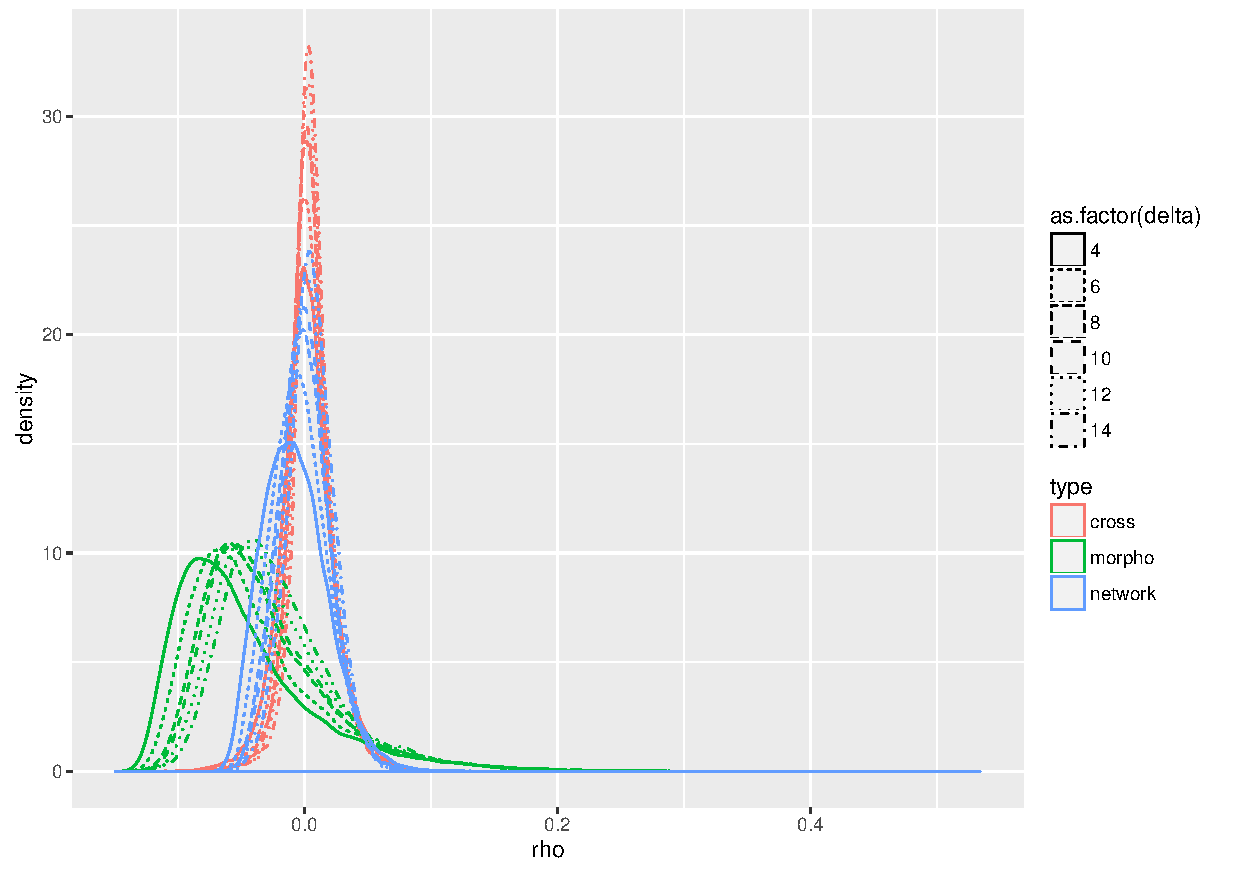
\includegraphics[width=0.33\textwidth]{figures/corrs-distrib_varyingdelta_bytype} % -> in supp material
%\includegraphics[width=0.5\textwidth]{figures/corrs-summary_varyingdelta_bytype_extended1}
%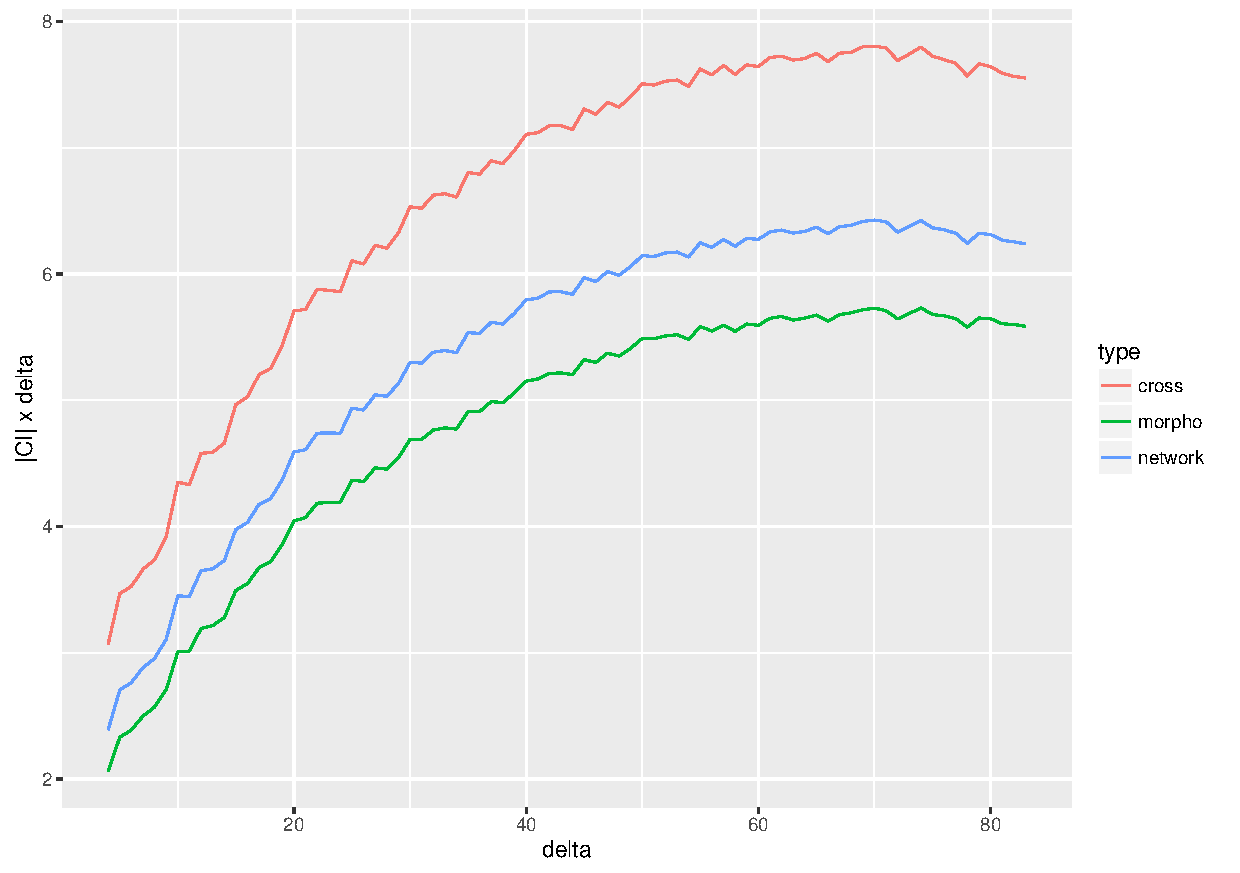
\includegraphics[width=0.5\textwidth]{figures/normalized_CI_delta}

\medskip

$\rightarrow$ Significant variation of mean correlation with $\delta$ (Left) and of normalized confidence interval (Right) given by $\left|\rho_+ - \rho_-\right|\cdot \delta$, as bounds theoretically vary as $\sqrt{N} \sim \sqrt{\delta^2}$ : implies multi-scalarity






Empirical Findings (Formalization)

$Y_i\left[\vec{x},t\right]$ spatio-temporal stochastic process, verifies empirically :

\bigskip

\begin{enumerate}
\item Local spatial autocorrelation is present and bounded by $l_{\rho}$ (in other words the processes are continuous in space) : at any $\vec{x}$ and $t$, $\left|\rho_{\norm{\Delta \vec{x}} < l_{\rho}}\left[Y_i (\vec{x}+\Delta \vec{x},t), Y_i (\vec{x},t) \right]\right| > 0$.
\medskip
\item Processes are locally parametrized : $Y_i = Y_i\left[\alpha_i\right]$, where $\alpha_i (\vec{x})$ varies with $l_{\alpha}$, with $l_{\alpha} \gg l_{\rho}$ and weakly locally stationary in space.
\medskip
%\item Spatial correlations between processes have a sense at an intermediate scale $l$ such that $l_{\alpha}\gg l \gg l_{\rho}$.
%\item Processes covariance stationarity times scale as $\sqrt{l}$.
%\item Local ergodicity is present at scale $l$ and dynamics are locally chaotic.
\item Processes are multi-scalar : since $\rho(\delta = \infty) > \rho (\delta = 0 )$, a necessary non-linear correction on processes spatial averages in correlation computation is present.
% add computation in supplementary materials / papers. -> later
\end{enumerate}



Analytical Deductions

1. \textbf{Regimes of temporal correlations.} Let assume local ergodicity in $\vec{x}_0$ at scale $\delta \cdot l_0$ (reasonable with urban growth and network extension in recent times). The Ergodic theorem implies that $\exists \mathcal{T}$ such that

\[<Y_i (t) >_{\norm{\vec{x}-\vec{x}_0} < \delta\cdot l_0} = <Y_i (\vec{x}_0)>_{t\in \mathcal{T}}\] 

With spatial stationarity, $<Y_i>_{\vec{x}_0}=<Y_i>_{\vec{x}_1}$, thus $\mathcal{T}$ must be constant to be invariant by translation. By contraposition and (2), processes have different dynamical characteristics.
% if translate in a given direction, looses a small part, must be compensated by the area translated by delta (overlap), thus must be constant.

\bigskip

2. \textbf{Global non-ergodicity.} Let $X_k$ a partition of space into local areas. We have $<\cdot>_x = \sum_k w_k <\cdot>_{x_k} =_{(1)} \sum_k w_k <\cdot>_{\mathcal{T}_k} $. On the other hand, global ergodicity would give $<\cdot>_t = <\cdot>_{\mathcal{T}} = \sum_k w_k <\cdot>_{\mathcal{T}}$ and $\sum_k w_k \left(<\cdot>_{\mathcal{T}} - <\cdot>_{\mathcal{T}_k}\right) = 0$. Being true on each subset implies $\mathcal{T}=\mathcal{T}_k$, what contradicts (1).





%
%
%%%%%%%%%%%%%%%%%%
%\sframe{Stationarity and Ergodicity}{
%
%\begin{itemize}
%\item Assuming local ergodicity, spatial local stationarity implies and temporal local stationarity
%
%\item Spatial non-stationarity \textbf{at the second order}$\implies$ temporal scale variations $\implies$ non-ergodicity
%
%\end{itemize}
%
%}
%




Case study : implications
% thematic conclusion of the case study on ergodicity

$\rightarrow$ Still points to explore :
\begin{itemize}
\item variable correlations areas (size and shape in space)
\item same work on cities population/train network data, which are also dynamical databases : extrapolation of ergodicity parameters ?
\item correlations of returns : link between $\rho\left[\Delta_t Y\right]$ and $\rho\left[\Delta_x Y\right]$ (more difficult : if pure local ergodicity, $\exists$ a permutation making the correspondance) % may be difficult to identify 
\item Link between $\Delta_{\delta}\rho (\delta)$ and process derivatives ?
\end{itemize}

\bigskip

$\rightarrow$ We show the regional nature of network-territories interactions, in particular the non-ergodicity of urban systems on \textbf{the interaction these components}

\bigskip

$\rightarrow$ No direct results on time dynamics, but indirect : spatio-temporal processes do not have same speed and react/diffuse differently









%%%%%%%%%%%%%%%%%%
\subsection{Application to China}{Application à la Chine}


\bpar{
Although \cite{zheng2014assessing} underlined a quick acceleration of OpenStreetMap road data completeness and accuracy, its use for computation of network indicators may be questioned. \cite{zhang2015density} highlights four regimes of data quality, partitioning China into regions among which qualitative behavior of OSM data varies. We choose in the following to work only on the regions where the quality is the highest, i.e. with high density and high diversity. % TODO precise which areas
For density data, we use the gridded population data from~\cite{fu1km}. % TODO check also that
}{

}







%%%%%%%%%%%%%%%%%%
%\subsection{Insights for interaction processes}













%----------------------------------------------------------------------------------------


\newpage

\section[Disentangling co-evolutions from causal relations]{Disentangling co-evolutions from causal relations : a case study on \emph{Bassin Parisien}}{Isoler la Co-évolution des Relations causales}

Spatial statistics studies on dynamical relations between network and territories are relatively rare. \cite{levinson2008density} does so on London metropolitan area and identifies causalities using lagged variables, but does not disentangle relations in the sense of coupled statistical models that would isolate endogenous effects from coupling effects.

 % study on london with temporal and spatial lag (weird use of spatial statistics) -> expected conclusions but does not really disentangle ?



\subsection{Context Formalization}{Formalisation}

%\subsubsection{Variables}

%\paragraph{Description}

We assume a dynamic transportation network $n(\vec{x},t)$ within a dynamic territorial landscape $\vec{T}(\vec{x},t)$, which components are to simplify population $p(\vec{x},t)$ and employments $e(\vec{x},t)$. Data is structured the following way :
\begin{itemize}
\item Observation of territorial variables are discretized in space and in time, i.e. the spatial field $\vec{T}$ is summarized by $\mathbf{T} = \left(\vec{T}(\vec{x}_i,t_j^{(T)})\right)_{i,j}$ with $1\leq i \leq N$ and $1\leq j \leq T$. They concretely correspond to census on administrative units (\emph{communes} in our case) at different dates.
\item Network has a continuous spatial position but is represented by the vector of network distances $\mathbf{N}$
\end{itemize}



%\paragraph{Definitions}



\subsection{On Accessibility}{Sur l'accessibilité}

% accessibility : need to introduce it ?
%  -> read Weibull

The notion of accessibility has been central to regional science since its introduction and systematization in planning around 1970. 

%\paragraph{Existence of accessibility}

%An elegant axiomatic definition is derived in~\cite{weibull1976axiomatic}. Starting from expected properties of an accessibility function $A$ that associate a value to \emph{attraction} $a$ and distance $d$, defined on the set of discrete spatial configurations $\mathcal{C} = \cup_{n\in \mathbb{N}}{(d_i,a_i)_{1\leq i \leq n}}$. These properties include (among technical others with no thematic meaning) :
%\begin{enumerate}
%\item $A$ is invariant regarding the order of the configuration
%\item $A$ decrease with distance at fixed attraction and increase with attraction at fixed distance
%\item $A$ is invariant when adding null attractions and constant configurations
%\end{enumerate}

%A canonical decomposition of any accessibility function 


As already introduced in the first chapter, we question the notion of accessibility : \textit{Is the notion of accessibility crucial for statistical analysis ?}

\medskip


Weibull has proposed an axiomatic approach to accessibility~\cite{weibull1976axiomatic}, deriving a canonical decomposition for any \emph{attraction-accessibility} function $A(a,d)$, assuming expected thematic axioms among others technical ones that are :
\begin{enumerate}
\item $A$ is invariant regarding the order of the configuration
\item $A$ decrease with distance at fixed attraction and increase with attraction at fixed distance
\item $A$ is invariant when adding null attractions and constant configurations
\end{enumerate}
Then $A$ verifies these if and only if it is of the form

\[
A\left[(a_i,d_i)\right] = T\left(\bigoplus_i z(d_i,a_i)\right)
\]

where $T$ is increasing with null origin, $z$ is a \emph{distance substitution function} (i.e. verifying axiom 2) and $\oplus$ a \emph{standard composition} associating two attractions at zero distance to th corresponding unique one. 

It means that well suited matrices of autocorrelation should capture accessibility in regressions ; or it must be captured by non-linear regression on $\mathbf{N}$. It may reveal some kind of intrinsic accessibility that is related to real phenomena (that we expect to fit with calibrated functions of accessibility based on Hedonic models e.g.) Seeing accessibility as a potential field is an equivalent vision : given any stationary dynamic for $n,\vec{T}$, Helmoltz theorem states that it derives from a potential (can be adapted to non-stationary dynamics with a time-varying potential).

%\paragraph{Continuous approach and accessibility potential}

% Paul : Helmoltz-Hodge theorem to infer potential field from speed spatial field ?
%  Q : what are trajectories ? dirac field has no rotational -> continuous approach does not work ?


\subsection{Data}{Données}

We will work on a novel dataset provided by \noun{Le Nechet}, that consists in main road infrastructures with their opening dates and train network for network dynamics, and in population and employments of communes at census dates, for Bassin Parisien on the last fifty year. The temporal granularity due to census temporal step may be an obstacle to obtain good dynamical statistics.


\subsection{Statistical Tests}{Tests Statistiques}


The following large set of analysis are to be tested (non exhaustive) :
\begin{itemize}
\item On raw data :
\begin{itemize}
\item Multivariate models
\[\mathcal{L}\left[\mathbf{T},\mathbf{N}\right]\sim \varepsilon\]
\item Autocorrelated univariate models
\[(\mathbf{I} - \Sigma R W) \mathbf{X} \sim \varepsilon\]
\item Autocorrelated multivariate models \[(\mathcal{L}' - \Sigma R W)\left[\mathbf{T}+\mathbf{N}\right] \sim \varepsilon\]
\item Geographically Weighted Regression~\cite{brunsdon1998geographically}
\[
\mathcal{L}\left[\mathcal{G}\left(\mathbf{T},\mathbf{N}\right)\right] \sim \varepsilon
\]
\item Granger causality tests : \cite{xie2009streetcars} use for example Granger causality to link transit with land-use changes.
\end{itemize}
\item On data returns :
\begin{itemize}
\item Autoregressive multivariate models
\[\mathcal{L}\left[(\Delta \mathbf{T}(t_{j'}))_{j'\leq j},(\Delta \mathbf{N}(t_{j'}))_{j'\leq j}\right] \sim \varepsilon\]
\item Autoregressive autocorrelated multivariate models : idem with spatial autocorrelation term.
\item Synthetic Instrumental Variables : static territory and/or network ?
\end{itemize}
\end{itemize}



%\subsubsection{Bivariate linear models}

%\subsubsection{Autocorrelated univariate models}

%\subsubsection{Autocorrelated multivariate models}

%\subsubsection{Granger causality tests}

%\cite{xie2009streetcars} use Granger causality to link transit with land-use changes.

%\subsubsection{Autoregressive multivariate models}

%\subsubsection{Autoregressive autocorrelated multivariate models}


\bigskip

%\subsection{Expected results}

%We expect from these analyses to test at these spatial and temporal scales, and on a particular metropolitan case study, the assumption on network necessity for the territorial system of functional job commutings.




%%%%%%%%%%%%%%%%%%
\subsection{Generic Method}{Méthode Générique}

% TODO introduce here systematic granger causality testing - first tests on RBD ?


\subsubsection{Description}{Description}


\bpar{
We describe here a generic method, based on a test similar to Granger causality test~\cite{}, aiming to identify causal relations in spatial systems. Let $X_j(\vec{x},t)$ unidimensional spatial random processes. A realization of a territorial subsystem is given by set of trajectories for each process $x_{i,j,t}$. We assume the existence of correspondance functions $\Phi_{j1,j2}$ that associate realizations of each components to a unique index (in the simplest case, variables on the same patch will be associated). If $\textrm{argmax}_{\tau} \hat{\rho}\left[x_{j1},x_{j2}\right]$ is clearly defined, its sign will then give the sense of the causality between components $j1$ and $j2$.
}{
Nous décrivons ici une méthode générique, basée sur un test similaire à la causalité de Granger~\cite{}, pour tenter d'identifier des relations causales dans des systèmes spatiaux. Soit $X_j(\vec{x},t)$ des processus aléatoires spatiaux unidimensionnels. Une réalisation d'un sous-système territorial est donnée par des ensembles de trajectoires pour chaque processus $x_{i,j,t}$. On suppose l'existence de fonctions de correspondance $\Phi_{j1,j2}$ permettant de faire correspondre les réalisations de chaque composantes à un index unique (dans le cas le plus simple, on associera les variables sur les mêmes patches). Si $\textrm{argmax}_{\tau} \hat{\rho}\left[x_{j1},x_{j2}\right]$ est clairement défini % TODO notion trop floue ? le problème est que des modèles stat conditionnent trop ?
, son signe donnera alors le sens de la causalité entre les composantes $j1$ et $j2$.
}

% TODO some kind of smoothing has to be introduced, either as preprocessing or as part of the optimization process (at least for first observed behavior on synthetic data. maybe it is typical of the model ?)
% - formalize mean estimator on repetitions, compare it to a direct estimator (// computation or aggregated data ?)


\cite{luo2013spatio} : Spatio-temporal Granger causality for fMRI data ; not really spatial in the sense that no real distance effect.



\subsubsection{Synthetic Data}{Données Synthétiques}


\paragraph{Case study}{Etude de cas}

Cette méthode doit dans un premier temps être testée et partiellement validée, ce que nous proposons de faire sur des données synthétiques, approche dont l'utilisation est documentée et illustrée au chapitre~\ref{}. \cite{raimbault2014hybrid} est un modèle simple de morphogenèse urbaine (modèle RBD) faisant un candidat intéressant pour notre test. En effet, les variables explicatives de la croissance urbaine, les processus d'extension du réseau et le couplage entre densité urbaine et réseau sont assez élémentaires. Cependant, hormis dans des cas extrêmes (distance au centre détermine valeur foncière uniquement, le réseau dépendra de manière causale de la densité, ou distance au réseau seule, la causalité devrait être inversée), les régimes mixtes n'exhibent pas de causalités évidentes : c'est donc un parfait cas pour tester si la méthode est capable d'en détecter.


\paragraph{Application}{Application}

Nous explorons une grille de l'espace des paramètres du modèle RBD. Pour chaque valeur des paramètres, nous procédons à $N=$ répétitions. Le modèle a par ailleurs été exploré de nouveau pour reproduction et extension des résultats. % TODO appendice with RBD exploration.



%----------------------------------------------------------------------------------------

\newpage

\section[Real Estate Trajectories]{Early warnings of Network Breakdowns : socio-economic and real estate trajectories}{Trajectoires de Marchés Immobiliers}


\subsection{Context}{Contexte}



\bpar{
Various aspects of territories are concerned by interactions with networks. In previous empirical studies, no socio-economic attributes of populations inhabiting the territory nor economic values for land and real estate was considered. Both are however crucial elements of territorial dynamics and are extensively studied in fields such as territorial analysis or urban economics : for example, \cite{homocianu:tel-00359302} studies households residential choices to understand land-use transportation interactions. We propose here to use a database of Real Estate transactions for Parisian region on the last 20 years, with 2 years temporal granularity and exact spatial coordinates. \cite{guerois2009dynamique} used it to make typologies of spatial dynamics of Parisian real estate. This project is conjointly done with \noun{Le Corre} whose strong thematic knowledge on Real Estate financial properties will bring insight for spatial typologies of temporal trajectories.% results using base bien.
}{
Des aspects très variés des territoires sont concernés par l'interaction avec les réseaux. Dans nos études précédentes, aucun aspect socio-économique des populations habitant le territoire ni des valeurs économiques pour le foncier et l'immobilier n'ont été considérés. Il s'agit cependant d'éléments cruciaux des dynamiques territoriales et sont étudiés de manière intensive dans des champs comme l'analyse territoriale ou l'économie urbaine : par exemple, \cite{homocianu:tel-00359302} étudie les choix résidentiels des ménages pour comprendre les interactions entre usage du sol et transport. Nous proposons ici d'utiliser une base de données de transactions immobilières pour la région parisienne sur les 20 dernières années, avec une granularité temporelle de 2 ans et coordonnées spatiales exactes. \cite{guerois2009dynamique} l'utilise pour établir une typologie des dynamiques spatiales du marché immobilier parisien.
}


\subsection{Preliminary Results}{Résultats Préliminaire}


We show in Fig.~\ref{fig:realestate} typologies of temporal transactional profiles for total stocks. Temporal dynamics show different reactions of local territories to the 2008 crisis, in particular a strong differentiation between urban and rural areas. More precise classification into urban territories are still to be investigated when the analysis will be pushed further.



%%%%%%%%%%%%%%%
\begin{figure}
\hspace{-3cm}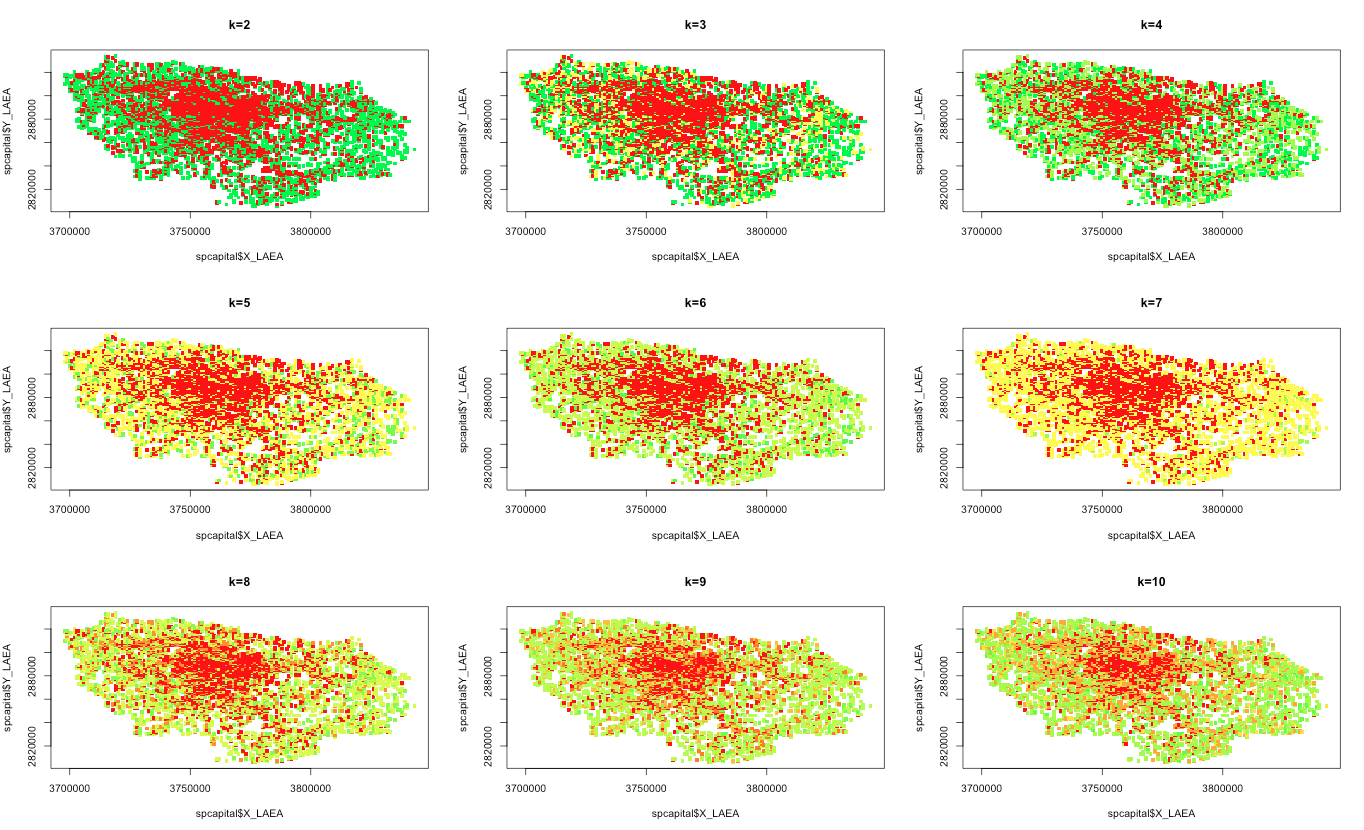
\includegraphics[width=1.4\textwidth]{Figures/PartII/Empirical/RealEstate/normalized_k2-10}
\smallskip
\hspace{-3cm}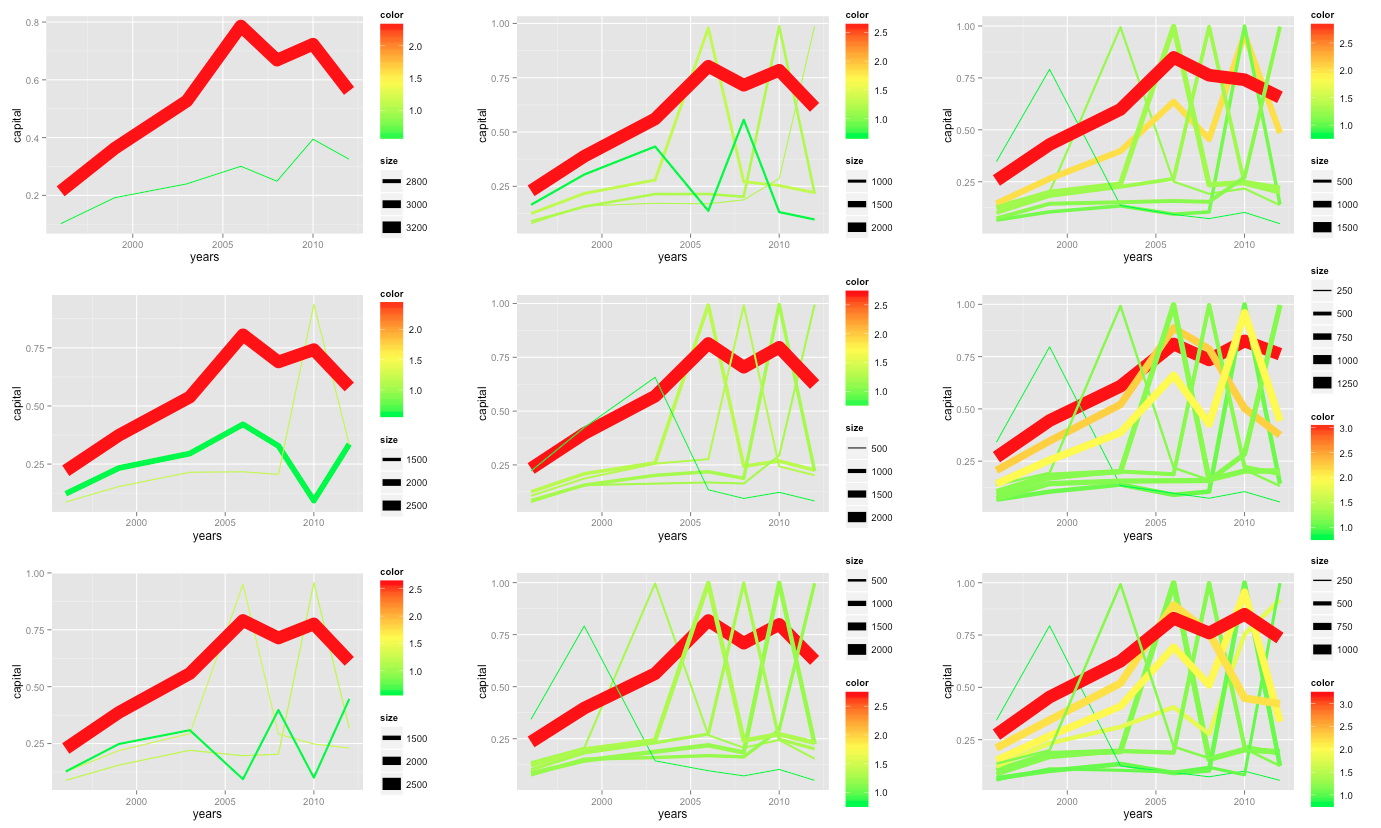
\includegraphics[width=1.4\textwidth]{Figures/PartII/Empirical/RealEstate/trajectories_normalized_k=2-10}
\caption[Typology of Real Estate trajectories]{Typology of Real Estate trajectories. Locations were categorized using averaged k-means on time-series. We show maps and time series for value of k from 2 to 10.}{}
\label{fig:realestate}
\end{figure}
%%%%%%%%%%%%%%%



\subsection{A strategy to investigate early warnings of network breakdowns}{Une Stratégie pour étudier les signes précurseurs de rupture de potentiels}


The span of the end of this database coincides with planification phases of the Grand Paris Express that we already mentioned. We aim to seek for early warnings of potential station implantation, in correspondance with different stages of the project, in order to verify if intrinsic territorial dynamics were already present or if the announcement of a new station induced a local phase transition.





%----------------------------------------------------------------------------------------

\newpage

\section[South-African historical events as instruments]{South-African historical events as instruments to understand network-territory relations}{Relations Réseaux-territoires en Afrique du Sud}

\subsection{Context}{Contexte}


\noun{Baffi} studied in her thesis project~\cite{baffi2016thesis} qualitatively the role of South African railways in segregations and integration processes, aims to use an extensive database of railway growth and population dynamics in cities on the last 100 years produced during the thesis. In particular, she showed qualitatively that dynamics between territories and networks profoundly changed at the end of the apartheid, transforming a tool of sordid planned segregation (network shaped was optimized to minimize unwanted accessibility) into an integration tool thanks to recent changes in network topology patterns.

\subsection{Objectives}{Objectifs}

We can use first the particular shape of that network to control on local and global topology effects (but this is quite equivalent as controlling on accessibility), and in a second time the historical events as statistic instruments, assuming that territorial dynamics and network dynamics responded differently to these. We expect to learn from these project informations on interactions at long time scale and large spatial scale, in a very particular context of constrained growth.






\subsection{Possible developments}{Développements possibles}


The method of instruments in statistics~\cite{angrist1996identification} is used to identify causal relationships between variables, in a different way than Granger causality test for example. Trying to identify causalities between network dynamics and territorial dynamics is of crucial importance to test our theoretical assumption on the existence of co-evolution.











%%%%%%%%%%%%%%%
% Toy modeling : density model / correlated synthetic data



% Chapter 

\chapter{Modeling} % Chapter title

\label{ch:modeling} % For referencing the chapter elsewhere, use \autoref{ch:name} 





%----------------------------------------------------------------------------------------

\headercit{Do or do not. There is no try.}{Yoda}{}


\bigskip


One does not simply \emph{try} to model something. On that point personal experience confirms indeed that point, as I remember as an early Master student giving in to the call of incautious agent-based modeling, naively thinking that integrated models of any aspect of an urban system could be constructed, producing numerous NetLogo code lines to build a gaz factory with unfounded internal processes, an extremely poor external validation and no internal validation. This was a try and therefore a step towards the dark side of models bricolage. The construction of a computational model of simulation is a rigorous exercise that one can not improvise, as much as statistical modeling. Recent progresses in the field~\cite{banos2013pour} help to that purpose, and modular model construction and validation is one tool useful to avoid becoming lost in shady places.

We propose in this chapter simple modeling experiments, conceived to be preliminaries for more elaborated tests of our theory. We begin with a simple diffusion-aggregation model of urban growth as a relatively small scale. Beginning with simple assumptions does not mean a non-rigorous exploration of the model, that is therefore explored and calibrated on real data. The fact that we reproduce existing urban forms without the use of networks suggest either the total absence of network influence at this scale, or its very strong influence yielding apparent random effects that disappear in average calibration. We propose then to simply couple this model with a network generation heuristic in order to study feasible correlations between morphology and network. The absence of coupled calibration avoids to draw empirical conclusion but the method is satisfying in itself as it permits the generation of synthetic territorial configurations where correlation structure is controlled. We finally describe a project of benchmark of diverse heuristic models for network generation.





%----------------------------------------------------------------------------------------

\newpage


% Q : synthetic data to be mentioned here ? 
%    -> may be in Methodology
%    then needs to clarify : Plan (of course) ; diagram for plan ; and dependence tree for parts/sections




%---------------------------------------------------

\newpage

\section{Urban Morphogenesis by Aggregation-diffusion}{Morphogenèse Urbaine par Agrégation-diffusion}

\label{sec:densitygeneration}


%---------------------------------------------------



\bpar{
We study a stochastic model of urban growth generating spatial distributions of population densities at an intermediate mesoscopic scale. The model is based on the antagonist interplay between the two opposite abstract processes of aggregation (preferential attachment) and diffusion (urban sprawl). Introducing indicators to quantify precisely urban form, the model is first statistically validated and intensively explored to understand its complex behavior across the parameter space. We then compute real morphological measures on local areas of size 50km covering all European Union, and show that the model can reproduce most of existing urban morphologies in Europe. It implies that the morphological dimension of urban growth processes at this scale are sufficiently captured by the two abstract processes of aggregation and diffusion.
}{
Nous étudions un modèle stochastique de croissance urbain générant des distribution spatiales de densité de population à une échelle intermédiaire mesoscopique. Le modèle se base sur le jeu antagoniste entre les deux processus abstrait opposé de l'agrégation (attachement préférentiel) et de la diffusion (étalement urbain). En utilisant des indicateurs pour quantifier précisément la forme urbaine, le modèle est d'abord validé statistiquement puis exploré intensivement pour comprendre son comportement complexe sur son espace de paramètres. Ayant calculé précédemment les mesures morphologiques réelles sur des aires locales de taille 50km couvrant l'ensemble de l'Union Européenne, nous les utilisons pour montrer que le modèle peut reproduire la plupart des morphologies urbaines existantes en Europe. Cela implique que la dimension morphologique des processus de croissance urbaine à cette échelle est capturée de manière suffisante par les deux processus abstraits d'agrégation et de diffusion.
}


\subsection{Context}{Contexte}


\bpar{
The study of urban growth, and more particularly its quantification, is more than ever a crucial issue in a context where most of the world population live in cities which expansion has significant environmental impacts~\cite{seto2012global} and that have therefore to ensure an increased sustainability and resilience to climate change. The understanding of drivers for urban growth can lead to better integrated policies. It is however a question far from being solved in the diverse related disciplines: Urban Systems are complex socio-technical systems that can be studied from a large variety of viewpoints. Batty has advocated in that sense for the construction of a dedicated science defined by its objects of study more than the methods used~\cite{batty2013new}, what would allow easier coupling of approaches and therefore Urban Growth models taking into account heterogeneous processes. The processes that a model can grasp are also linked to the choice of the scale of study. At a macroscopic scale, models of growth in system of cities are mainly the concern of economics and geography. \cite{gabaix1999zipf} shows that in first approximation, the Gibrat's model postulating random growth rates not depending on city size, yield the well-know Zipf's law, or rank-size law, which is a typical stylized fact witnessing hierarchy in systems of cities. It was however shown empirically that systematic deviations to this law exist~\cite{rozenfeld2008laws}, and that spatial interactions may be responsible for it. Models integrating spatial interactions include for example \cite{bretagnolle2000long} that introduces a growth model in which these interactions, that are function of distance and the geography, play a significant role in growth rates. More recently, \cite{favaro2011gibrat} has extended this model by taking into account innovation waves between cities as a driver. The interplay of space, economic and population growth is studied by the Marius model~\cite{cottineau2014evolution} in the case of the former Soviet Union, on which model performance is shown improved compared to models without interactions.
}{
L'étude de la croissance urbaine, et plus particulièrement sa quantification, est plus que jamais un enjeu crucial dans un contexte ou la majorité de la population mondiale vit dans des villes dont l'expansion a des impacts environnementaux significatifs~\cite{seto2012global} et qui doivent pour cela assurer une soutenabilité et une résilience au changement climatique accrues. La compréhension des moteurs de la croissance urbaine devrait conduire à l'élaboration de politiques mieux intégrées. Il s'agit cependant d'une question loin d'être résolue dans les diverses disciplines concernées: les systèmes urbains sont des systèmes socio-techniques complexes qui peuvent être étudiés d'une grande variété de points de vue. \noun{Batty} défend en ce sens la construction d'une science dédiée définie par ses objets d'étude plus que par les méthodes utilisées~\cite{batty2013new}, ce qui devrait permettre des couplages plus faciles entre approches et donc des modèles de croissance urbaine prenant en compte des processus hétérogènes. Les processus qu'un modèle peut prendre en compte sont également liés au choix de l'échelle d'étude. A une échelle macroscopique, les modèles de croissance pour les systèmes de villes sont majoritairement le sujet de l'économie et de la géographie. \cite{gabaix1999zipf} montre qu'en première approximation, le modèle de Gibrat postulant des taux de croissance aléatoires ne dépendant pas de la taille des villes, produit la bien connue loi de Zipf, ou loi rang-taille, qui est un fait stylisé typique témoignant d'une hiérarchie dans les systèmes de villes. Il a cependant été démontré empiriquement que des déviations systématiques à cette loi existent~\cite{rozenfeld2008laws}, et que les interactions spatiales pourraient en être responsables. Les modèles intégrant les interactions spatiales incluent par exemple \cite{bretagnolle2000long} qui introduit un modèle de croissance dans lequel ces interactions, qui sont fonction de la distance et de la géographie, jouent un rôle significatif dans les taux de croissance. Plus récemment, \cite{favaro2011gibrat} a étendu ce modèle en prenant en compte les vagues d'innovation entre les villes comme facteur d'influence. Les relations entre espace, croissance économique et croissance de la population sont étudiées par le modèle Marius~\cite{cottineau2014evolution} pour le cas de l'ex-Union Soviétique, pour lequel la performance du modèle est démontrée améliorée par rapport aux modèles sans interactions.
}

\bpar{
At smaller scales, that can be understood as microscopic or mesoscopic depending on the resolution and extent of models, agents of models fundamentally differ. Space is generally taken into account in a finer way, through neighborhood effects for example. For example, \cite{andersson2002urban} propose a micro-based model of urban growth, with the purpose to replace non-interpretable physical mechanisms with agent mechanisms, including interactions forces and mobility choices. Local correlations are used in \cite{makse1998modeling}, which develops the model introduced in~\cite{makse1995modelling}, to modulate growth patterns to ressemble real configurations. The world of Cellular Automata (CA) models of Urban Growth~\cite{batty1994cells} also offers numerous examples. \cite{GEAN:GEAN940} introduced a generic framework for CA with multiple land use, based on local evolution rules. A model with simpler states (occupied or not) but taking into account global constraints is studied by \cite{ward2000stochastically}. The Sleuth model, initially introduced by \cite{clarke1998loose} for the San Francisco Bay area, and for which an overview of diverse applications is given in~\cite{clarke2007decade}, was calibrated on areas all over the world, yielding comparative measures through the calibrated parameters.
}{
A de plus petites échelles, qui peuvent être comprises comme microscopiques ou mesoscopiques selon la résolution et l'étendue spatiale des modèles, les agents des modèles diffèrent fondamentalement. L'espace est généralement pris en compte de manière plus fine, par les effets de voisinage par exemple. Par exemple, \cite{andersson2002urban} un modèle de croissance urbaine basé sur le microscopique, dans le but de remplacer des mécanismes physiques non interprétables par des mécanismes d'agents, incluant des forces d'interaction et des choix de mobilité. Les corrélations locales sont utilisées par \cite{makse1998modeling}, qui développe le modèle introduit dans \cite{makse1995modelling}, pour moduler les motifs de croissance pour qu'ils ressemblent à des configurations réelles. Le monde des modèles de croissance urbaine à automates cellulaires (CA)~\cite{batty1994cells} offre aussi de nombreux exemples. \cite{GEAN:GEAN940} introduit un cadre générique pour les CA avec usage du sol multiple, basé sur des règles d'évolution locales. Un modèle avec des états plus simples (occupé ou non) mais prenant en compte des contraintes globales est étudié par~\cite{ward2000stochastically}. Le modèle Sleuth, introduit initialement par~\cite{clarke1998loose} pour la zone de la Baie de San Francisco, et pour lequel un aperçu des diverses applications est donné dans~\cite{clarke2007decade}, a été calibré sur des régions tout autour du monde, fournissant des mesures comparatives au travers des paramètres calibrés.
}


\bpar{
Closely related to CA models but not exactly similar are Urban Morphogenesis models, which aim to simulate the growth of urban form from autonomous rules. \cite{frankhauser1998fractal} suggested that the fractal nature of cities is closely linked to the emergence of the form from the microscopic socio-economic interactions, namely urban morphogenesis. \cite{courtat2011mathematics} develops a morphogenesis model for urban roads alone, with growth rules based on geometrical considerations. These are shown sufficient to produce a broad range of patterns analog to existing ones. Similarly, \cite{raimbault2014hybrid} couples a CA with an evolving network to reproduce stylized urban form, from concentrated monocentric cities to sprawled suburbs. The Diffusion-Limited-Aggregation model, coming from physics, and which was first studied for cities by~\cite{batty1991generating}, can also be seen as a morphogenesis model. These kind of models, that sometimes can be classified as CA, have generally the particularity of being parsimonious in their structure.
}{
Assez proches des modèles CA, mais pas exactement similaires, sont les modèles de Morphogenèse Urbaine, qui visent à simuler la croissance de la forme urbaine à partir de règles autonomes. \cite{frankhauser1998fractal} suggère que la nature fractale des villes est en relation étroite avec l'émergence de la forme urbaine à partir des interactions socio-économiques microscopiques, à savoir la morphogenèse urbaine. \cite{courtat2011mathematics} développe un modèle de morphogenèse pour les routes urbaines seules, avec des règles de croissance basées sur des considérations géométriques. Celles ci sont montrées suffisantes pour produire un large spectre de motifs analogues à des existants. De manière similaire, \cite{raimbault2014hybrid} couple un CA avec un réseau évolutif pour reproduire des formes urbaines stylisées, de villes monocentriques concentrées à des banlieues étalées. Le modèle Diffusion-Limited-Aggregation, venant de la physique, et qui a été appliqué aux villes en premier par~\cite{batty1991generating}, peut aussi être vu comme un modèle de morphogenèse. Ce type de modèles, qui peuvent parfois être classifiés comme CA, ont généralement la particularité d'être parcimonieux dans leur structure. Des modèles similaires ont également été étudiés en biologie pour la diffusion de population par exemple~\cite{bosch1990velocity}.
}


\bpar{
We study in this section a morphogenesis model, at the mesoscopic scale, aimed at being simplistic in its rules and variables, but trying to be accurate in the reproduction of existing patterns. The underlying question is to explore the performance of simple mechanisms in reproducing complex urban patterns. We consider abstract processes, namely aggregation and diffusion, candidates as partially explanatory drivers of urban growth, based on population only, that will be detailed in model rationale below. An important aspect we introduce is the quantitative measure of urban form, based on a combination of morphological indicators, to quantify and compare model outputs and real urban patterns. Our contribution is significant on several points: (i) we compute local morphological characteristics on a large spatial extent (full European Union); (ii) we give significant insights into model behavior through extensive exploration of the parameter space; (iii) we show through calibration that the model is able to reproduce most of existing urban forms across Europe, and that these abstract processes are sufficient to explain urban form alone. The rest of this paper is organized as follows: we first describe formally the model and the morphological indicators. We then detail values of morphological measures on real data, study the behavior of the model by exploring its parameter space and through a semi-analytical approach to a simplified case, and we describe results of model calibration.
}{
Nous étudions dans cette section un modèle de morphogenèse, à l'échelle mesoscopique, dont le but est d'être simple dans ses règles et variables, mais visant à être performant pour la reproduction de motifs existants. La question sous-jacente est l'exploration de la performance de mécanismes simples pour reproduire des formes urbaines complexes. Nous considérons des processus abstrait, précisément l'agrégation et la diffusion, comme candidats comme facteurs potentiellement explicatifs de la croissance urbaine, basés sur la densité de population seule, qui seront détaillés ci-dessous. Un aspect important que nous utilisons est la mesure quantitative de la forme urbaine, basée sur une combinaison d'indicateurs morphologiques, pour quantifier et comparer les sorties de modèle et les formes urbaines réelles. Notre contribution est significative sur plusieurs points: (i) le calcul des caractéristiques morphologiques réelles sur une étendue spatiale conséquente (Union Européenne complète); (ii) nous apprenons le comportement du modèle par une exploration conséquente de l'espace des paramètres; (iii) nous montrons par la calibration que le modèle est capable de reproduire la majorité des formes urbaines existantes en Europe, et que ces processus abstraits sont suffisants pour expliquer la forme urbaine seule. La suite de cette section est organisée de la façon suivante : nous décrivons d'abord formellement le modèle. Nous étudions ensuite le comportement du modèle par une exploration de l'espace des paramètres et par une approche semi-analytique d'un cas simplifié, puis nous décrivons les résultats de la calibration du modèle.\comment[FL]{revue de litt pas assez hierarchisee}
}





\subsection{Model and Results}{Modèle et Résultats}



\subsubsection{Urban growth model}{Modèle de croissance urbaine}




%%%%%%%%%%%%%%%%%%%%%%%%
\paragraph{Rationale}{Description}

\bpar{
Our model is based on widely accepted ideas of diffusion-aggregation processes for Urban Processes. The combination of attraction forces with repulsion, due for example to congestion, already yield a complex outcome that has been shown under some simplifying assumptions to be representative of urban growth processes. A model capturing these processes was introduced by~\cite{batty2006hierarchy}, as a cell-based variation of the DLA model~\cite{batty1991generating}. Indeed, the tension between antagonist aggregation and sprawl mechanisms may be an important process in urban morphogenesis. For example \cite{fujita1996economics} opposes centrifugal forces with centripetal forces in the equilibrium view of urban spatial systems, what is easily transferable to non-equilibrium systems in the framework of self-organized complexity: a urban structure is a far-from-equilibrium system that has been driven to this point by these opposite forces. The two contradictory processes of urban concentration and urban sprawl are captured by the model, what allows to reproduce with a good precision a large number of existing morphologies. We can expect aggregation mechanisms such as preferential attachment to be good candidates in urban growth explanation, as it was shown that the Simon model based on them generates power-laws typical of urban systems (scaling laws for example)~\cite{2016arXiv160806313S}. The question at which scale is it possible and relevant to define and try to simulate urban form is rather open, and will in fact depend on which issues are being tackled. Working in a typical setting of morphogenesis, the processes considered are local and our model must have a resolution at the micro-level. We however want to quantify urban form on consistent urban entities, and will work therefore on spatial extents of order 50$\sim$100km. We sum up these two aspects by stating that the model is at the \emph{mesoscopic scale}.
}{
Notre modèle est basé sur des idées largement acceptées de processus d'agrégation-diffusion pour les les processus urbains. La combinaison de forces d'attraction avec celles de répulsion, dues par exemple à la congestion, fournit déjà une issue complexe qui a été montrée représentative des processus de croissance urbaine sous certaines hypothèses simplificatrices. Un modèle capturant ces processus a été introduit dans~\cite{batty2006hierarchy}, comme une variation cellulaire du modèle DLA~\cite{batty1991generating}. En effet, la tension entre les mécanismes antagonistes d'agrégation et d'étalement peut être un processus important pour la morphogenèse urbaine. Par exemple, \cite{fujita1996economics} oppose les forces centrifuges aux forces centripètes dans une vision d'équilibre des systèmes urbains spatiaux, ce qui peut facilement être transféré aux systèmes hors équilibre dans le cadre de la complexité auto-organisée: une structure urbaine est un système \emph{far-from-equilibrium} qui a été conduit à ce point par ces forces opposées. Les deux processus contradictoires de concentration urbaine et d'étalement urbain sont capturés par le modèle, ce qui permet de reproduire avec une bonne précision un grand nombre de morphologies existantes. Nous pouvons supposer que des mécanismes d'agrégation comme l'attachement préférentiel sont des bons candidats pour expliquer la croissance urbaine, puisqu'il a été montré que le modèle de Simon qui se base dessus génère des \emph{power-law} qui sont typiques des systèmes urbains (lois d'échelles par exemple)~\cite{2016arXiv160806313S}. La question de l'échelle à laquelle il est possible et pertinent de définir et d'essayer de simuler la croissance urbaine est relativement ouverte, et dépendra en fait de quels problèmes sont considérés. Travaillant dans un cadre typique de la morphogenèse, les processus considérés sont locaux et notre modèle doit avoir une résolution au niveau microscopique. Nous voulons cependant quantifier la forme sur des unités urbaines cohérentes, et travaillerons ainsi sur des étendues spatiales d'ordre 50$\sim$100km. Nous résumons ces deux aspects en posant que le modèle est à l'échelle \emph{mesoscopique}.
}

\paragraph{Formalization}{Formalisation}

\bpar{
We formalize now the model and its parameters. The world is a square grid of width $N$, in which each cell is characterized by its population $(P_i(t))_{1\leq i\leq N^2}$. We consider the grid initially empty, i.e. $P_i(0)=0$, but the model can be easily generalized to any initial population distribution. The population distribution is updated in an iterative way. At each time step,
}{
Nous formalisons à présent le modèle et ses paramètres. Le monde est une grille carrée de côté $N$, dans lequel chaque cellule est caractérisée par sa population $(P_i(t))_{1\leq i\leq N^2}$. Nous considérons la grille initialement vide, i.e. $P_i(0)=0$, mais le modèle peut être facilement généralisé à n'importe quelle distribution initiale de population. La distribution de population est mise à jour de façon itérative. A chaque pas de temps,
}

\bpar{
\begin{enumerate}
\item Total population is increased by a fixed number $N_G$ (growth rate). Each population unit is attributed independently to a cell following a preferential attachment such that 
\begin{equation}
\Pb{P_i(t+1)=P_i(t)+1|P(t+1)=P(t)+1}=\frac{(P_i(t)/P(t))^{\alpha}}{\sum(P_i(t)/P(t))^{\alpha}}
\end{equation}
The attribution being uniformly drawn if all population are equal to 0.
\item A fraction $\beta$ of population is diffused to cell neighborhood (8 closest neighbors receiving each the same fraction of the diffused population). This operation is repeated $n_d$ times.
\end{enumerate}
}{
\begin{enumerate}
\item La population totale est augmentée par un nombre fixe $N_G$ (taux de croissance). Chaque unité de population est attribuée indépendamment à une cellule suivant un attachement préférentiel tel que
\begin{equation}
\Pb{P_i(t+1)=P_i(t)+1|P(t+1)=P(t)+1}=\frac{(P_i(t)/P(t))^{\alpha}}{\sum(P_i(t)/P(t))^{\alpha}}
\end{equation}
L'attribution est tirée de manière uniforme si toutes les populations sont égales à 0.
\item Une fraction $\beta$ de la population est diffusée au voisinage de chaque cellule (les 8 plus proches voisins recevant chacun la même fraction de la population diffusée). Cette opération est répétée $n_d$ fois.
\end{enumerate}
}

\bpar{
The model stops when total population reaches a fixed parameter $P_m$. To avoid bord effects such as reflecting diffusion waves, border cells diffuse their due proportion outside of the world, implying that the total population at time $t$ is strictly smaller than $N_G\cdot t$.
}{
Le modèle s'arrête que la population totale atteint un paramètre fixé $P_m$. Pour éviter les effets de bord comme des ondes de diffusion se réfléchissant, les cellules du bord diffusent la proportion qu'elles devraient hors du monde, ce qui implique que la population totale à l'instant $t$ est strictement plus petite que $N_G\cdot t$.
}

\bpar{
We summarize model parameters in Table~\ref{tab:density:parameters}, giving the associated processes and values ranges we use in the simulations. The total population of the area $P_m$ is exogenous, in the sense that it is supposed to depend on macro-scale growth patterns on long times. Growth rate $N_G$ captures both endogenous growth rate and migration balance within the area. The aggregation rate $\alpha$ sets the differences in attraction between cells, what can be understood as an abstract attraction coefficient following a scaling law of population. Finally, the two diffusion parameters are complementary since diffusing with strength $n_d\cdot \beta$ is different of diffusing $n_d$ times with strength $\beta$, the later giving flatter configuration.
}{
Nous résumons les paramètres du modèle dans la Table~\ref{tab:density:parameters}, donnant les processus associés et les bornes des valeurs utilisées dans les simulations. La population totale de la zone $P_m$ est exogène, au sens qu'elle est supposée dépendre de processus de croissance à l'échelle macroscopique sur le temps long. Le taux de croissance $N_G$ capture à la fois la croissance endogène et la balance migratoire dans la zone. Le taux d'agrégation $\alpha$ fixe la différence d'attractivité entre cellules, qui peut être interprétée comme un coefficient abstrait d'attraction suivant une loi d'échelle de la population. Enfin, les deux paramètres de diffusion sont complémentaires puisque diffuser avec force $n_d\cdot \beta$ est différent de diffuser $n_d$ fois avec force $\beta$, le dernier cas donnant des configurations plus plates.
}

% table summarizing parameters
%  $\alpha \in [0.1,4],\beta \in [0,0.5],n_d \in \{1,\ldots , 5\}, N_G \in [500,30000], P_m \in [1e4,1e6]$
%%%%%%%%%%%%%
\begin{table}[!ht]
\caption[Summary of model parameters][Résumé des paramètres]{\textbf{Summary of model parameters.}\label{tab:density:parameters}}{\textbf{Résumé des paramètres}\label{tab:density:parameters}}
\begin{tabular}{|l|l|l|l|}
\hline
Paramètre & Notation & Processus & Domaine\\ \hline
Population totale & $P_m$ & Croissance macroscopique & $[1e4,1e6]$\\ \hline
Taux de croissance & $N_G$ & Croissance mesoscopique  & $[500,30000]$\\ \hline
Force d'agrégation & $\alpha$ & Agrégation & $[0.1,4]$\\ \hline
Force de diffusion & $\beta$ & Diffusion & $[0,0.5]$\\ \hline
Nombre de diffusions & $n_d$ & Diffusion & $\{1,\ldots , 5\}$\\ \hline
\end{tabular}
\end{table}
%%%%%%%%%%%%%%


\paragraph{Measuring the Urban Form}{Mesure de la forme urbaine}

\bpar{
As our model is only density-based, we propose to quantify its outputs through spatial morphology, i.e. properties of the spatial distribution of density. At the scale chosen, these will be expected to translate various functional properties of the urban landscape. 
}{
Comme le modèle se base uniquement sur la densité, nous proposons de quantifier ses sorties par la morphologie spatiale, i.e. les propriétés de la distribution spatiale de la densité. A l'échelle choisie, on s'attend à ce qu'elle traduise diverse propriétés fonctionnelles de l'environnement urbain. Le contexte et la définition des indicateurs a déjà été donnée en section~\ref{sec:staticcorrelations}.
}


\subsubsection{Real data}{Données réelles}


Nous travaillons sur les valeur des indicateurs calculées en section~\ref{sec:staticcorrelations} pour l'Europe, sur les fenêtres de côté 50km avec résolution de 100 cellules. Nous posons donc pour la suite $N=100$ pour les simulations du modèle.





%%%%%%%%%%%%%%%%%%%%%%%%
\subsubsection*{Generation of urban patterns}{Génération de structures urbaines}


\paragraph{Implementation}{Implémentation}

\bpar{
The model is implemented both in NetLogo~\cite{wilensky1999netlogo} for exploration and visualization purposes, and in \texttt{Scala} for performance reasons and easy integration into OpenMole~\cite{reuillon2013openmole}, which allows a transparent access to High Performance Computing environments. Computation of indicator values on geographical data is done in \texttt{R} using the \texttt{raster} package~\cite{hijmans2015geographic}. Source code and results are available on the open repository of the project at \texttt{https://github.com/JusteRaimbault/Density}. Raw datasets for real indicator values and simulation results are available on Dataverse at \texttt{http://dx.doi.org/10.7910/DVN/WSUSBA}.
}{
Le modèle est implémenté à la fois en NetLogo~\cite{wilensky1999netlogo} pour des raisons d'exploration et de visualisation, et en \texttt{Scala} pour des raisons de performance et d'intégration plus aisée dans OpenMole~\cite{reuillon2013openmole}, qui permet un accès transparent aux environnements de calcul haute performance. Le calcul des valeurs des indicateurs sur les données géographiques est fait en \texttt{R} avec le package \texttt{raster}~\cite{hijmans2015geographic}. Le code source et les résultats sont disponibles sur le dépôt ouvert du projet\footnote{à \texttt{https://github.com/JusteRaimbault/Density}}. Les données des valeurs réelles des indicateurs et des résultats de simulation sont disponibles sur Dataverse\footnote{à \texttt{http://dx.doi.org/10.7910/DVN/WSUSBA}}. Nous avons dans le cadre de l'implémentation \texttt{Scala} implémenté la convolution de distribution en deux dimension par Transformée de Fourier rapide, permettant de transformer une complexité $O(N^4)$ en $O(N^2\log^2 N)$, puis implémenté les indicateurs qui ont pu être intégrés à une extension NetLogo dédiée~\ref{app:subsec:morphologyextension}.
}

\paragraph{Generated Shapes}{Formes générées}


\bpar{
The model has a relatively small number of parameters but is able to generate a large variety of shapes, extending beyond existing forms. In particular, its dynamical nature allows through the interplay between $P_m$ and $N_G$ parameter to choose between final configurations that can be non-stationary or semi-stationary, whereas the interplay between $\alpha$ and $\beta$ modulates the sprawl and the compactness of forms. We run the model for parameters varying in ranges given in Table~\ref{tab:parameters}, for a world size $N=100$. Fig.~\ref{fig:fig2} shows examples of the variety of generated shapes for different parameter values, with corresponding interpretations. The four very different shapes can be obtained with variation of a single parameter sometimes: going from a peri-urban area from a rural area implies an increased aggregation at the same level of diffusion. Note that the model is density driven, and that the parameter $P_m/N_G$ is what really influences the dynamics: the values of $P_m$ are in some cases not directly corresponding to the interpretations we made (for the rural in particular) that are done on densities. A rescaling keeps the settlement form and solves this issue. These examples show the potentiality of the model to produce diverse shapes. We need then to systematically tackle its stochasticity and explore its parameter space.
}{
Le modèle a un nombre relativement faible de paramètres mais est capable de générer une grande variété de formes, qui s'étendent au delà des formes existantes. Plus particulièrement, sa nature dynamique permet par la combinaison des paramètres $P_m$ et $N_G$ de choisir entre des configurations qui peuvent être non stationnaires ou semi stationnaires, tandis que l'interaction entre $\alpha$ et $\beta$ module l'étalement et le caractère compact des formes. Nous simulons le modèle pour des valeurs de paramètres variant dans les bornes données en Table~\ref{tab:density:parameters}, pour une taille de monde $N=100$. Fig.~\ref{fig:density:fig2} montre des exemples de la variété des formes urbaines générées pour différentes valeurs des paramètres, avec les interprétations correspondantes. Parmi les quatre formes très différentes, certaines peuvent être obtenues avec la variation d'un seul paramètre seulement : passer d'une zone péri-urbaine à une zone rurale implique une agrégation accrue au même niveau de diffusion. Il faut noter que le modèle est basé sur la densité, et que le paramètre $P_m/N_G$ est celui qui influence réellement la dynamique: les valeurs de $P_m$ ne correspondent dans certains cas pas directement aux interprétations qui en sont faites (pour le rural en particulier) qui sont faites sur les densités. Une homothétie garde la forme des établissements et résout ce problème. Ces exemples montrent la potentialité du modèle à produire des formes diverses. Nous devons ensuite étudier systématiquement sa stochasticité et explorer son espace des paramètres.
}


%%%%%%%%%%%%%
\begin{figure}
%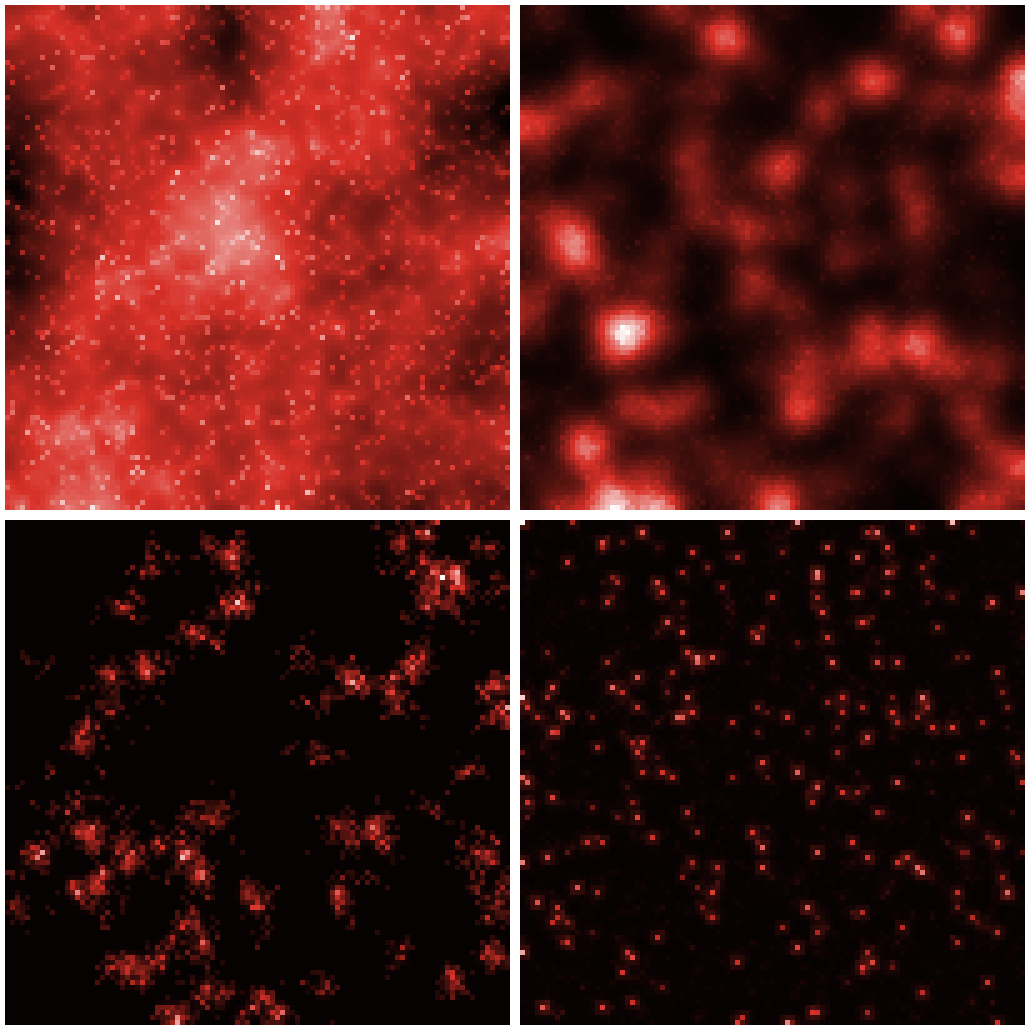
\includegraphics[width=\linewidth]{Figures/Density/Fig2}
%ex_sp-diffusion=0.05_sp-growth-rate=76_sp-diffusion-steps=2_sp-alpha-localization=0.4_ticks=995_sp-population=75620.00000000015.png
%ex_sp-diffusion=0.047_sp-growth-rate=274_sp-diffusion-steps=2_sp-alpha-localization=1.4_ticks=197_sp-population=53977.999999999935.png
%ex_sp-diffusion=0.0060_sp-growth-rate=25_sp-diffusion-steps=1_sp-alpha-localization=0.4_ticks=176_sp-population=4400.000000000003.png
%ex_sp-diffusion=0.0060_sp-growth-rate=268_sp-diffusion-steps=1_sp-alpha-localization=1.6_ticks=285_sp-population=76376.00000000033.png
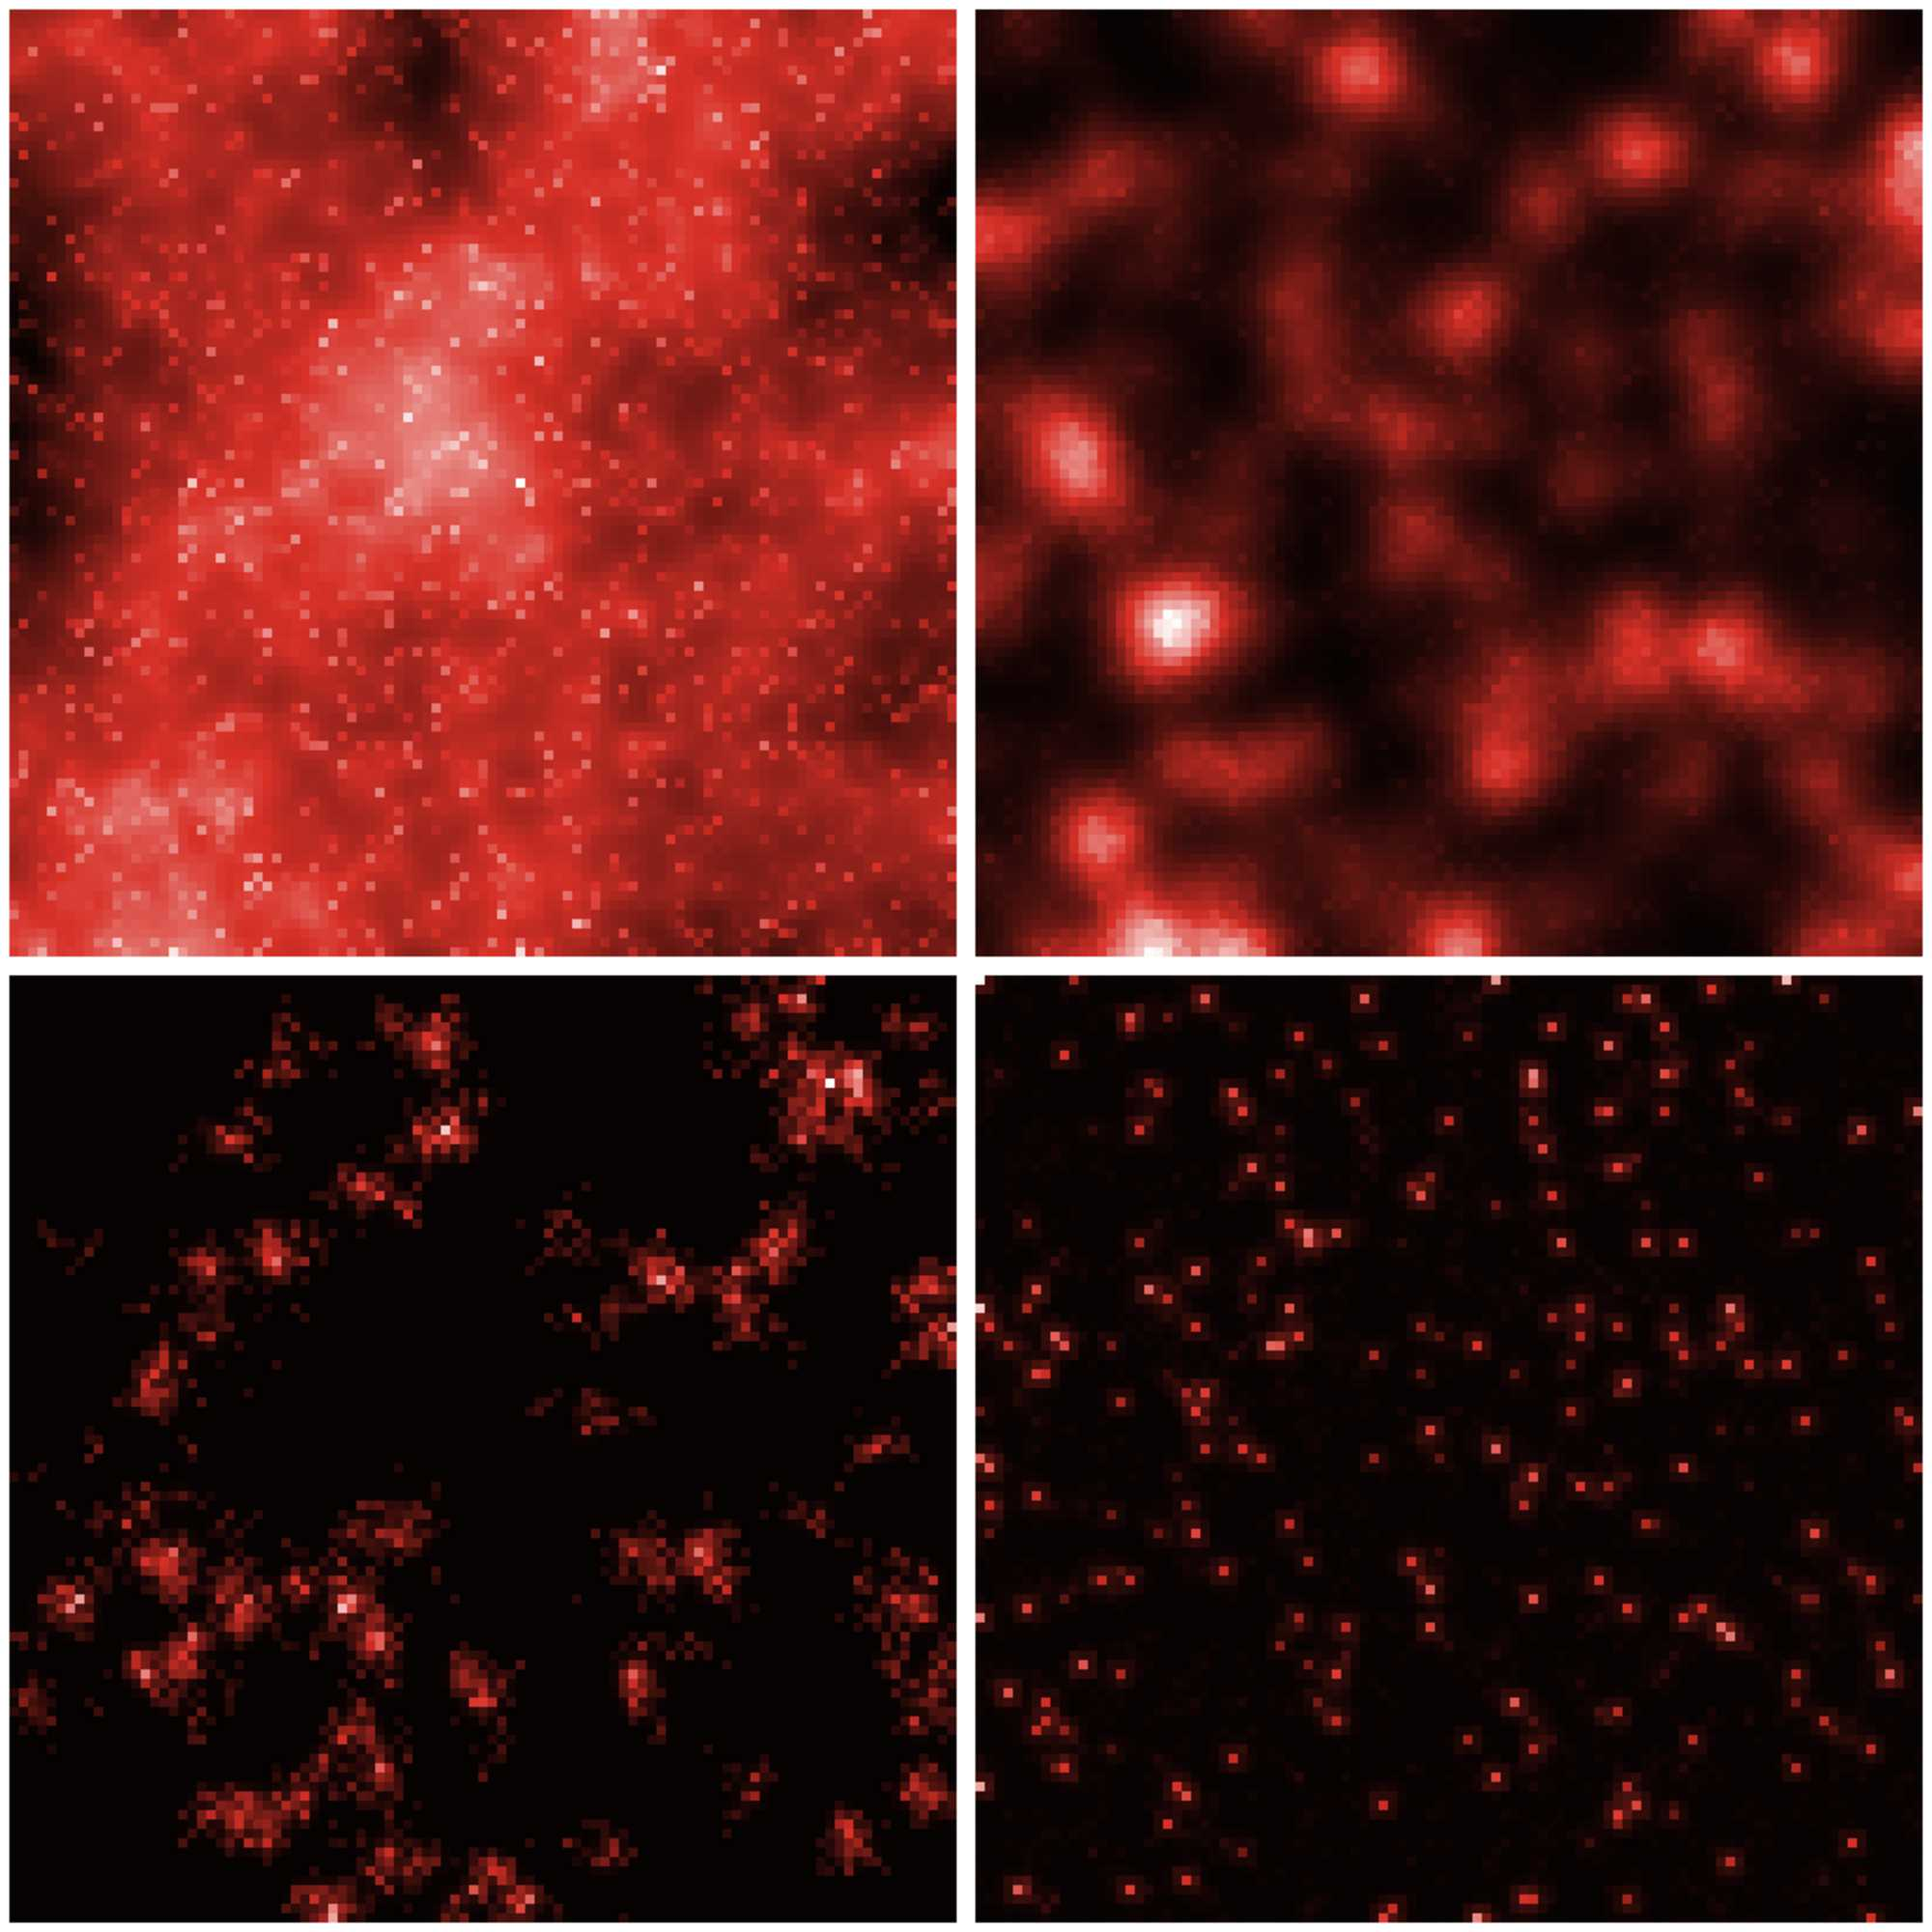
\includegraphics[width=\linewidth]{Figures/Final/5-2-2-fig-density-fig2}
\caption[Example of the variety of generated urban shapes][Exemple de formes urbaines générées]{\textbf{Example of the variety of generated urban shapes.} \textit{(Top left)} Very diffuse urban configuration, $\alpha = 0.4,\beta = 0.05, n_d = 2, N_G = 76, P_m = 75620$; \textit{(Top Right)} Semi-stationary polycentric urban configuration, $\alpha = 1.4,\beta = 0.047, n_d = 2, N_G = 274, P_m = 53977$; \textit{(Bottom Left)} Intermediate settlements (peri-urban or densely populated rural area), $\alpha = 0.4,\beta = 0.006, n_d = 1, N_G = 25, P_m = 4400$; \textit{(Bottom Right)} Rural area, $\alpha = 1.6,\beta = 0.006, n_d = 1, N_G = 268, P_m = 76376$.\label{fig:density:fig2}}{\textbf{Exemple de la variété de \emph{formes territoriales} générées.} \textit{(Haut Gauche)} Configuration urbaine très diffuse, $\alpha = 0.4,\beta = 0.05, n_d = 2, N_G = 76, P_m = 75620$; \textit{(Haut Droite)} Configuration polycentrique urbaine semi-stationnaire, $\alpha = 1.4,\beta = 0.047, n_d = 2, N_G = 274, P_m = 53977$; \textit{(Bas Gauche)} Etablissements intermédiaires (périurbain ou zone rurale densément peuplée), $\alpha = 0.4,\beta = 0.006, n_d = 1, N_G = 25, P_m = 4400$; \textit{(Bas Droite)} Zone rurale, $\alpha = 1.6,\beta = 0.006, n_d = 1, N_G = 268, P_m = 76376$.\label{fig:density:fig2}}
\end{figure}
%%%%%%%%%%%%%




%%%%%%%%%%%%%%%%%%%%%%%%
\subsubsection{Model Behavior}{Comportement du modèle}


\bpar{
In the study of such a computational model of simulation, the lack of analytical tractability must be compensated by an extensive knowledge of model behavior in the parameter space~\cite{banos2013pour}. This type of approach is typical of what Arthur calls the \emph{Computational shift in modern science}~\cite{arthur2015complexity}: knowledge is less extracted through analytical exact resolution than through intensive computational experiments, even for ``simple'' models such as the one we study.
}{
Dans l'étude d'un tel model computationnel de simulation, le manque de traçabilité analytique doit être compensé par une connaissance extensive du comportement du modèle dans l'espace des paramètres~\cite{banos2013pour}. Ce type d'approche est typique de ce qu'\noun{Arthur} nomme le \emph{tournant computationnel dans la science moderne}~\cite{arthur2015complexity} : la connaissance est moins extraite de résolutions analytiques exactes que par des expériences de calcul intensif, même pour des modèles ``simples'' comme celui que nous étudions.
}

\paragraph{Convergence}{Convergence}


\bpar{
First of all we need to assess the convergence of the model and its behavior regarding stochasticity. We run for a sparse grid of the parameter space consisting of 81 points, with 100 repetitions for each point. Corresponding histograms are shown in~\nameref{S1_Text}. Indicators show good convergence properties: most of indicators are easily statistically discernable across parameter points, and these are distinguished without ambiguity when taking into account all indicators. We use this experiment to find a reasonable number of repetitions needed in larger experiments. For each point, we estimate the Sharpe ratios for each indicators, i.e. mean normalized by standard deviation. The more variable indicator is Moran with a minimal Sharpe ratio of 0.93, but for which the first quartile is at 6.89. Other indicators have very high minimal values, all above 2. Its means than confidence intervals large as $1.5 \cdot \sigma$ are enough to differentiate between two different configurations. In the case of gaussian distribution, we know that the size of the 95\% confidence around the average is given by $2\cdot \sigma \cdot 1.96 / \sqrt{n}$, what gives $1.26 \cdot \sigma$ for $n=10$. We run therefore this number of repetitions for each parameter point in the following, what is highly enough to have statistically significant differences between average as shown above. In the following, when referring to indicator values for the simulated model, we consider the ensemble averages on these stochastic runs.
}{
Dans un premier temps il est important d'assurer la convergence du modèle et son comportement au regard de la stochasticité. Nous simulons le modèle pour une grille creuse de l'espace des paramètres contenant 81 points, avec 100 répétitions à chaque point. Les histogrammes correspondants sont montrés en Appendice~\ref{app:sec:density}. Les indicateurs présentent de bonnes propriétés de convergence: la plupart des indicateurs sont aisément discernable de manière statistique entre les points de paramètres, et ceux-ci sont distinguables sans ambiguité quand tous les indicateurs sont pris en compte. Nous utilisons cette expérience pour établir un nombre raisonnable de répétitions nécessaire pour des expériences plus volumineuses. Pour chaque point, nous estimons le ratio de Sharpe pour chaque indicateur, i.e. sa moyenne normalisée par la déviation standard. L'indicateur le plus variable est l'index de Moran avec un Sharpe minimal de 0.93, mais pour lequel le premier quartile est à 6.89. Les autres indicateurs ont tous des valeurs minimales très hautes, toutes au dessus de 2. Cela signifie que des intervalles de confiance large comme $1.5 \cdot \sigma$ sont suffisants pour différencier entre deux configurations différentes. Dans le cas d'une distribution Gaussienne, nous savons que la taille de l'intervalle de confiance à 95\% autour de la moyenne est donné par $2\cdot \sigma \cdot 1.96 / \sqrt{n}$, ce qui donne $1.26 \cdot \sigma$ pour $n=10$. Nous utilisons pour cela ce nombre de répétitions pour chaque point de paramètres par la suite, ce qui est largement suffisant pour avoir des différences entre les moyennes étant statistiquement signifiantes comme montré précédemment. Par la suite, lorsque nous considérons les valeurs des indicateurs pour le modèle simulé, nous considérons la moyenne d'ensemble sur ces répétitions stochastiques.  
}


% -> 10 repetitions give 1.24 \sigma : ok with these sharp

%       id       meanMoran            sdMoran           sharpeMoran        meanSlope      
% Min.   : 0   Min.   :0.0000997   Min.   :4.387e-05   Min.   : 0.9372   Min.   :-2.1220  
% 1st Qu.:20   1st Qu.:0.0026494   1st Qu.:3.055e-04   1st Qu.: 6.8929   1st Qu.:-1.0264  
% Median :40   Median :0.0102259   Median :1.024e-03   Median :10.0594   Median :-0.7326  
% Mean   :40   Mean   :0.0245863   Mean   :1.707e-03   Mean   :12.5250   Mean   :-0.7889  
% 3rd Qu.:60   3rd Qu.:0.0330126   3rd Qu.:2.469e-03   3rd Qu.:14.1114   3rd Qu.:-0.4594  
% Max.   :80   Max.   :0.1174664   Max.   :6.309e-03   Max.   :50.0461   Max.   :-0.1470  
%    sdSlope          sharpeSlope       meanEntropy       sdEntropy         sharpeEntropy      
% Min.   :0.001956   Min.   :  9.104   Min.   :0.2161   Min.   :4.852e-05   Min.   :    6.904  
% 1st Qu.:0.004311   1st Qu.: 17.323   1st Qu.:0.5240   1st Qu.:2.192e-04   1st Qu.:   18.503  
% Median :0.019704   Median : 40.997   Median :0.8685   Median :7.370e-03   Median :   69.986  
% Mean   :0.035573   Mean   : 57.884   Mean   :0.7529   Mean   :1.618e-02   Mean   : 3244.566  
% 3rd Qu.:0.047804   3rd Qu.: 72.753   3rd Qu.:0.9865   3rd Qu.:3.037e-02   3rd Qu.: 4479.465  
% Max.   :0.225275   Max.   :293.529   Max.   :0.9982   Max.   :5.675e-02   Max.   :20571.273  
%  meanDistance       sdDistance       sharpeDistance   
% Min.   :0.09208   Min.   :0.001579   Min.   :  1.922  
% 1st Qu.:0.44556   1st Qu.:0.002742   1st Qu.:  4.243  
% Median :0.89682   Median :0.020469   Median : 24.374  
% Mean   :0.68723   Mean   :0.050225   Mean   :152.769  
% 3rd Qu.:0.91474   3rd Qu.:0.105676   3rd Qu.:326.653  
% Max.   :0.92342   Max.   :0.182181   Max.   :579.846  





\paragraph{Exploration of parameter space}{Exploration de l'espace des paramètres}


\bpar{
We sample the Parameter space using a Latin Hypercube Sampling, with parameter as $\alpha \in [0.1,4],\beta \in [0,0.5],n_d \in \{1,\ldots , 5\}, N_G \in [500,30000], P_m \in [1e4,1e6]$. This type of cribbing is a good compromise to have a reasonable sampling without being subject to the dimensionality curse within normal computation capabilities. We sample around 80000 parameters points, with 10 repetitions each. Full plots of model behavior as a function of parameters are given in~\ref{app:sec:density}. We show in~\ref{fig:density:fig3} some particularly interesting behavior for slope $\gamma$ and average distance $\bar{d}$. First of all, the overall qualitative behavior depending on aggregation strength, namely that lower alpha giver less hierarchical and more spread configurations, confirms the expected intuitive behavior. The effect of diffusion strength $\beta$ is more difficult to grasp: the effect is inverted for slope between high and low growth rates but not for distance, that shows an inversion when $\alpha$ varies. In the low $N_G$ case, low diffusion creates more sprawled configuration when aggregation is low, but less sprawled when aggregation is high. Furthermore, all indicators show a more or less smooth transition around $\alpha \simeq 1.5$. Slope stabilize over certain values, meaning that the hierarchy cannot be forced more and indeed depends of the diffusion value, at least for low $N_G$ (right column). In general, higher valued for $P_m/N_G$ increase the effect of diffusion what could have been expected. The existence of a minimum for slope at $n_d=1,P_m/N_G\in\left[13,26\right]$ and lowest $\beta$ is unexpected and witnesses a complex interplay between aggregation and diffusion. The emergence of this ``optimal'' regime is associated with shifts of the transition points in other cases: for example, lowest diffusion imply a transition beginning at lower values of $\alpha$ for average distance. This exploration confirms that complex behavior, in the sense of unpredictable emerging forms, occurs in the model: one cannot say in advance the final form given some parameters, without referring to the full exploration of which we give an overview here.
}{
Nous échantillonnons l'espace des paramètres en utilisant un \emph{Latin Hypercube Sampling}, les paramètres variant dans $\alpha \in [0.1,4],\beta \in [0,0.5],n_d \in \{1,\ldots , 5\}, N_G \in [500,30000], P_m \in [1e4,1e6]$. Ce type de criblage est un bon compromis pour avoir un échantillonnage raisonnable sans être soumis au sort de la dimension dans des capacité de calcul normales. Nous échantillonnons autour de 80000 points, avec 10 répétitions chacun. Des graphes complets du comportement du modèle en fonction des paramètres sont donnés en~\ref{app:sec:density}. Nous montrons en Fig.~\ref{fig:density:fig3} des comportements particulièrement intéressants pour la pente $\gamma$ et la distance $\bar{d}$. Tout d'abord, le comportement qualitatif général en fonction de la force d'agrégation, c'est à dire que des valeurs faibles de $\alpha$ donnent des configurations moins hiérarchiques et plus étalées, confirme le comportement attendu intuitivement. L'effet de la force de diffusion $\beta$ est plus difficile à cerner: l'effet est inversé pour la pente entre des haut et bas taux de croissance mais pas pour la distance, qui elle présente une inversion quand $\alpha$ varie. Dans le cas où $N_G$ est faible, une diffusion faible crée des configuration plus étalée quand l'agrégation est basse, mais moins étalées quand l'agrégation est forte. De plus, tous les indicateurs présentent une transition plus ou moins abrupte autour de $\alpha \simeq 1.5$. La pente se stabilise au dessus de certaines valeurs, ce qui veut dire que la hiérarchie ne peut pas être forcée plus et dépend alors de la valeur de la diffusion, au moins pour les faibles $N_G$ (colonne de droite). En général, des valeurs fortes pour $P_m/N_G$ augmentent les effets de la diffusion ce à quoi on pouvait s'attendre. L'existence d'un minimum pour la pente à $n_d=1,P_m/N_G\in\left[13,26\right]$ et les valeurs faibles de $\beta$ est inattendue et témoigne d'une interaction complexe entre agrégation et diffusion. L'émergence de ce régime ``optimal'' est associé avec un décalage des points de transition dans les autres cas : par exemple une diffusion plus faible implique une transition commençant à des valeurs plus faible de $\alpha$ pour la distance. Cette exploration confirme qu'un comportement complexe, au sens de formes émergentes qui ne peuvent être prédites, est présent dans le modèle : il n'est pas possible de donner en avance la forme finale étant donné un jeu de paramètres, sans se référer à l'exploration complète dont nous avons donné un aperçu ici.
}



%%%%%%%%%%%%%
\begin{figure}
%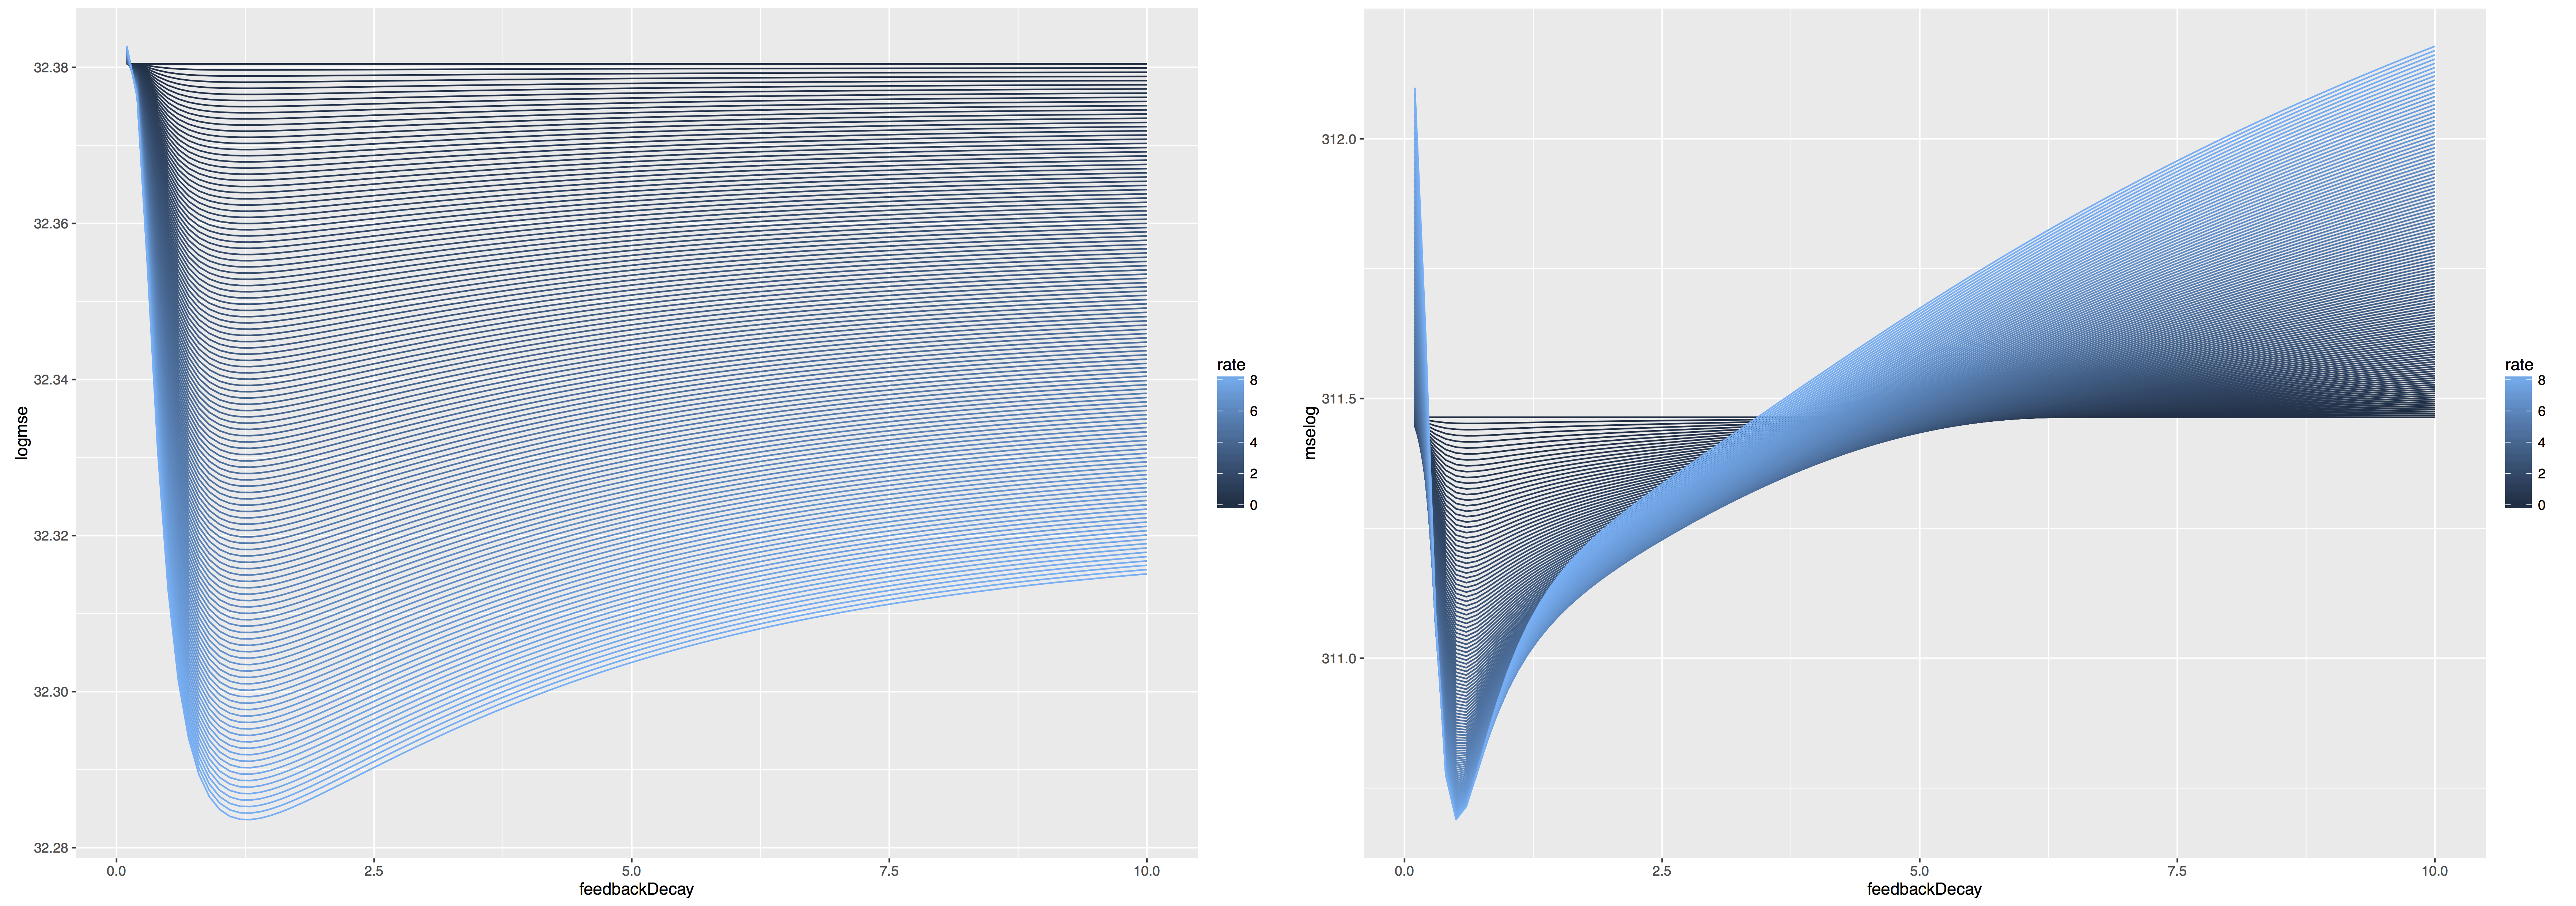
\includegraphics[width=\linewidth]{Figures/Density/Fig3.png}
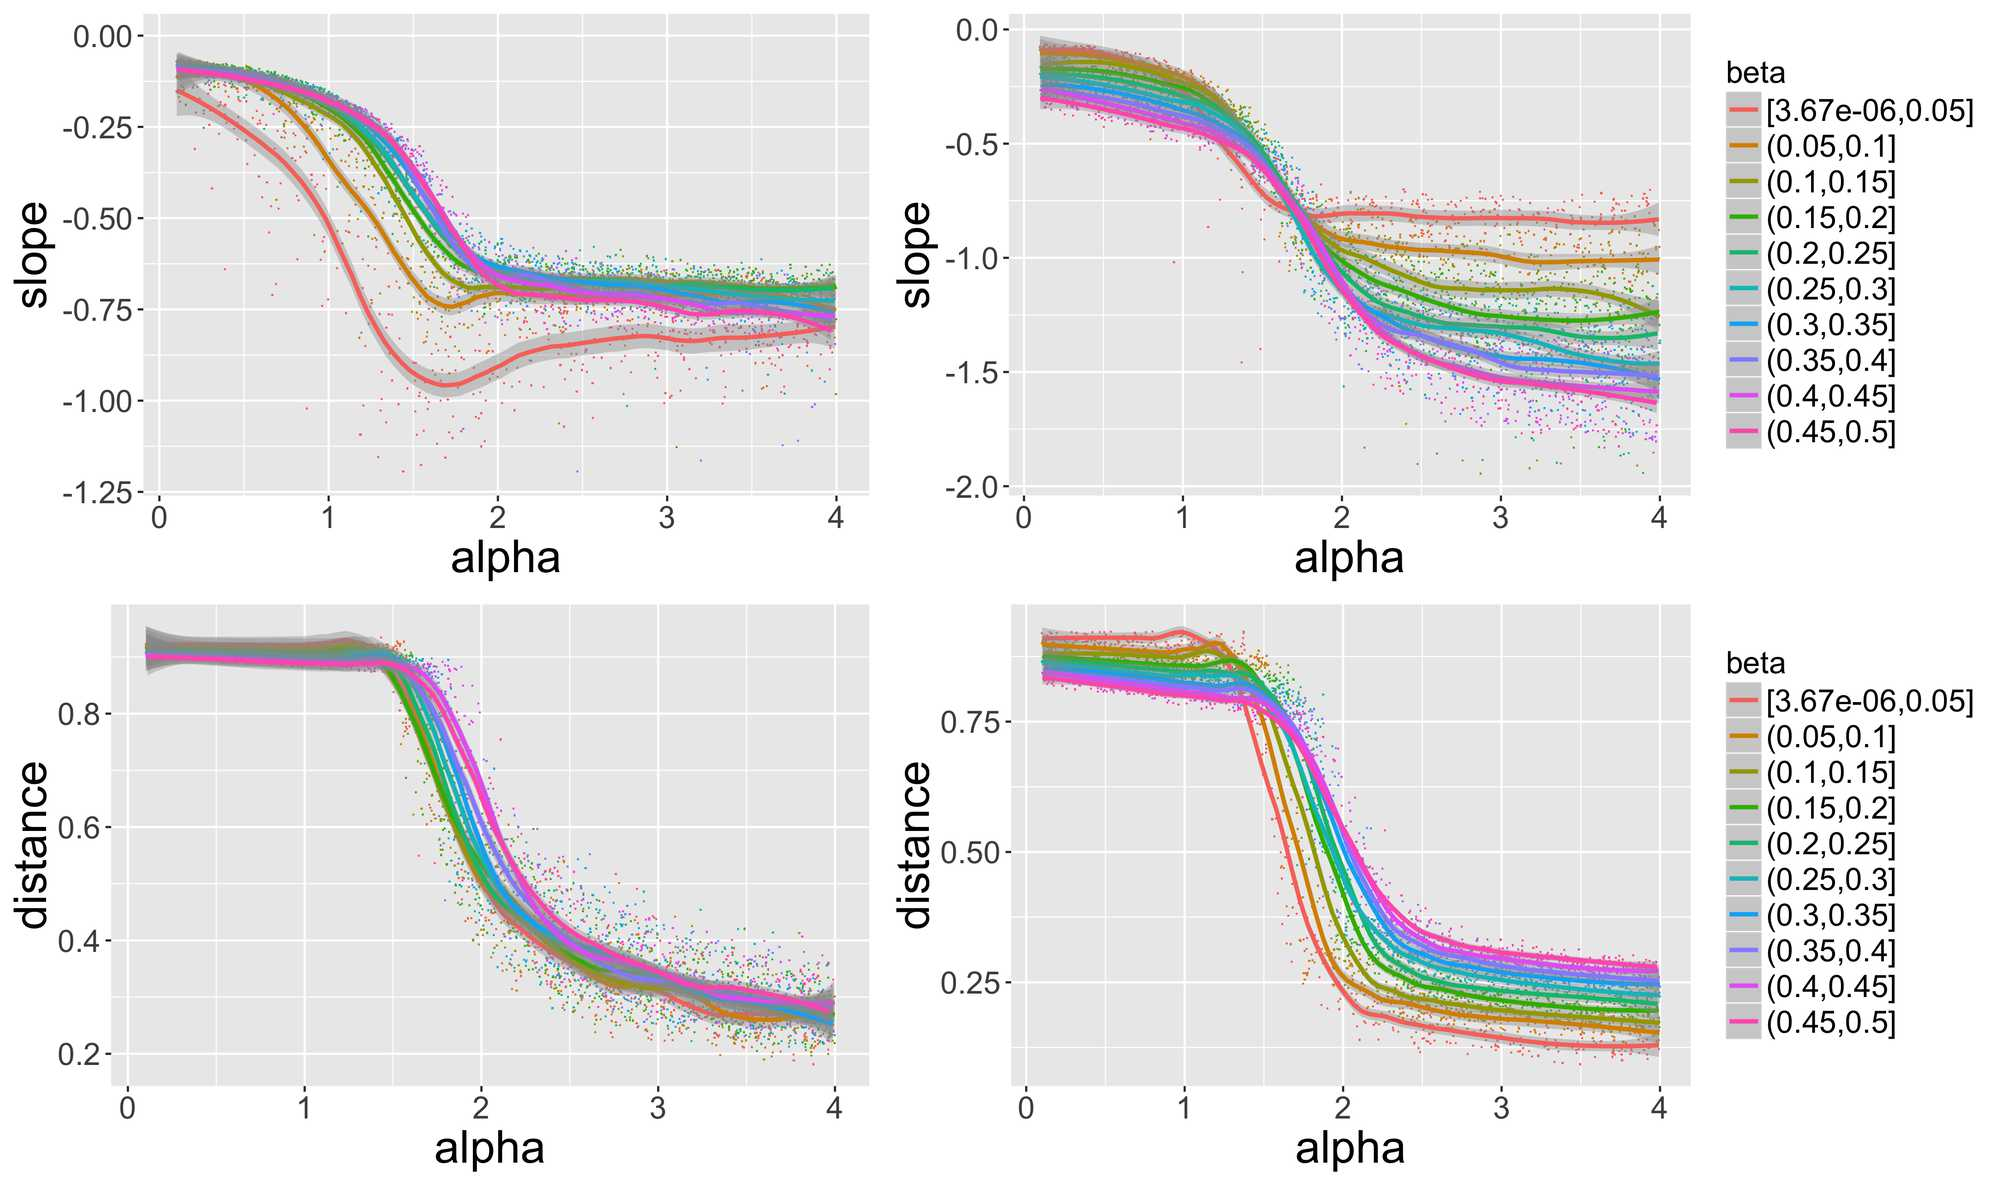
\includegraphics[width=\linewidth]{Figures/Final/5-2-2-fig-density-fig3}
\caption[Behavior of indicators][Comportement des indicateurs]{\textbf{Behavior of indicators.} Slope $\gamma$ (top row) and average distance $\bar{d}$ (bottom row) as a function of $\alpha$, for different bins for $\beta$ given by curve color, for particular values $n_d=1,P_m/N_G\in\left[13,26\right]$ (left column) and $n_d=4,P_m/N_G\in\left[41,78\right]$ (right column).\label{fig:density:fig3}}{\textbf{Comportement des indicateurs.} Pente $\gamma$ (ligne du haut) et distance moyenne $\bar{d}$ (ligne du bas) comme fonction de $\alpha$, pour différentes valeurs de $\beta$ données par la couleur des courbes, pour des valeurs particulières $n_d=1,P_m/N_G\in\left[13,26\right]$ (colonne de gauche) et $n_d=4,P_m/N_G\in\left[41,78\right]$ (colonne de droite). On observe dans chaque cas une transition en fonction de $\alpha$, dont les propriétés sont influencées par les autres paramètres. Pour les faibles valeurs de $P_m/N_G$ et de $\beta$ émerge une non-monotone contre intuitive.\label{fig:density:fig3}}
\end{figure}
%%%%%%%%%%%%%






%%%%%%%%%%%%%%%%%%%%%%%%
\subsubsection{Semi-analytical Analysis}{Analyse semi-analytique}


\bpar{
Our model can be understood as a type of reaction-diffusion model, that have been widely used in other fields such as biology: similar processes were used for example by Turing in its seminal paper on morphogenesis~\cite{turing1952chemical}. An other way to formulate the model typical to these approaches is by using Partial Differential Equations. We propose to gain insights into long-time dynamics by studying them on a simplified case. We consider the system in one dimension, such that $x\in \left[0;1\right]$ with $1/\delta x$ cells of size $\delta x$. A time step is given by $\delta t$. Each cell is characterized by its population as a random variable $P(x,t)$. We work on their expected values $p(x,t) = \Eb{P(x,t)}$, and assume that $n_d=1$. As developed in Supplementary Material~\ref{app:sec:density}, we show that this simplified process verifies the following PDE:
}{
Notre modèle peut être compris comme un type de modèle de réaction-diffusion, qui ont été utilisés largement dans d'autres champs comme la biologie: des processus similaires ont par exemple été utilisés par \noun{Turing} dans son article séminal sur la morphogenèse~\cite{turing1952chemical}. Une autre façon de formuler le modèle typique à ces approches est d'utiliser des Equations aux Dérivées Partielles (PDE). Nous proposons d'éclairer des comportements des dynamiques de temps long en les étudiant sur un cas simplifié. Nous considérons le système en une dimension, tel que $x\in \left[0;1\right]$ avec $1/\delta x$ cellule de taille $\delta x$. Un pas de temps est donné par $\delta t$. Chaque cellule est caractérisée par sa population comme une variable aléatoire $P(x,t)$.\comment[FL]{notations ne sont pas claires} Nous travaillons sur les espérances $p(x,t) = \Eb{P(x,t)}$, et supposons que $n_d=1$. Comme développé en Information Supplémentaire~\ref{app:sec:density}, on peut montrer que ce processus simplifié obéit à la PDE suivante :
}


\begin{equation}\label{eq:pde}
\hspace{-1.5cm}
\delta t \cdot \frac{\partial p}{\partial t} = \frac{N_G \cdot p^{\alpha}}{P_{\alpha}(t)} + \frac{\alpha \beta (\alpha - 1) \delta x^2}{2}\cdot \frac{N_G \cdot p^{\alpha-2}}{P_{\alpha}(t)} \cdot \left(\frac{\partial p}{\partial x}\right)^2 + \frac{\beta \delta x^2}{2} \cdot \frac{\partial^2 p}{\partial x^2} \cdot\left[ 1 + \alpha \frac{N_G p^{\alpha - 1}}{P_{\alpha(t)}} \right]
\end{equation}


\bpar{
where $P_{\alpha}(t) = \int_x p(x,t)^{\alpha} dx$. This non-linear equation can not be solved analytically, the presence of integral terms putting it out of standard methods, and numerical resolution must be used~\cite{tadmor2012review}. It is important to note that the simplified model can be expressed by a PDE analog to reaction-diffusion equations, as the one partially solved for a simpler model in~\cite{bosch1990velocity}. We show in \ref{app:sec:density} that because of the boundaries conditions, density (proportion of population) converges towards a stationary solution at long times, going through intermediate states in which the solution is partially stabilized, in the sense that its evolution speed becomes rather slow. These ``semi-stationary'' states are the ones used in two dimensions along with the dynamical ones. This study confirms that the variety of shapes obtained through the model is permitted both by the interplay of aggregation and diffusion as the equation couples them, but also by the values of $P_m / N_G$ that allow to set the convergence level. Indeed, the sensitivity of the stationary solution to parameters is very low compared to the shape of the world, and using the model in stationary mode would make no sense in our case. Finally, we use this toy case to demonstrate the importance of bifurcations in model dynamics. More precisely, we show that path-dependence is crucial for the final form. As illustrated in Fig.~\ref{fig:density:fig4}, using an initial condition making the choice ambiguous, corresponding to five equidistant equally populated cells, produces very different trajectories, as generally one of the spots will end dominating the others, but is totally random, witnessing dramatic bifurcations in the system at initial times. This aspect is typically expected in urban systems, and confirms the importance of robust indicators described before.
}{
où $P_{\alpha}(t) = \int_x p(x,t)^{\alpha} dx$. Cette équation non-linéaire ne peut pas être résolue analytiquement, la présence de termes intégraux la mettant hors des méthodes standard, et la résolution numérique doit être utilisée~\cite{tadmor2012review}. Il est important de noter que le modèle simplifié peut être exprimé comme une PDE analogue aux équations de réaction-diffusion, comme celle partiellement résolue pour un modèle plus simple dans~\cite{bosch1990velocity}. Nous montrons en \ref{app:sec:density} qu'à cause des conditions au bord, la densité (au sens de la proportion de population) converge vers une solution stationnaire sur le temps long, en passant par des états intermédiaires pour lesquels la solution est partiellement stabilisée, au sens où sa vitesse d'évolution devient relativement lente. Ces états ``semi-stationnaires'' sont ceux utilisés en deux dimensions avec les états dynamiques. Cette étude confirme que la variété des formes obtenue par le modèle est permise à la fois par l'interactions entre l'agrégation et la diffusion puisque l'équation les couple, mais aussi par les valeurs de $P_m / N_G$ qui permet de fixer le niveau de convergence. En effet, la sensibilité de la solution stationnaire aux paramètres est très faible en comparaison de la forme du monde (en écho à notre étude sur la sensibilité aux conditions spatiales initiales en~\ref{sec:computation}), et utiliser le modèle en mode stationnaire n'aurait aucun sens dans notre cas. Enfin, nous utilisons ce cas simplifié pour démontrer l'importance des bifurcations dans la dynamique du modèle. Plus précisément, nous montrons que la dépendance au chemin est cruciale pour la forme finale. Comme illustré en Fig.~\ref{fig:density:fig4}, l'utilisation d'une condition initiale rendant les choix ambigus, correspondant à 5 cellules équidistantes et de population égale, produit des trajectoires très différentes, puisqu'en général l'un des lieux finira par dominer les autres, mais est complètement aléatoire, témoignant de bifurcations cruciales dans le système aux instants initiaux. Cet aspect est typiquement attendu dans les systèmes urbains, et confirme l'importance d'indicateurs morphologiques robustes décrits précédemment.
}


%%%%%%%%%%%%%
\begin{figure}[h!]
%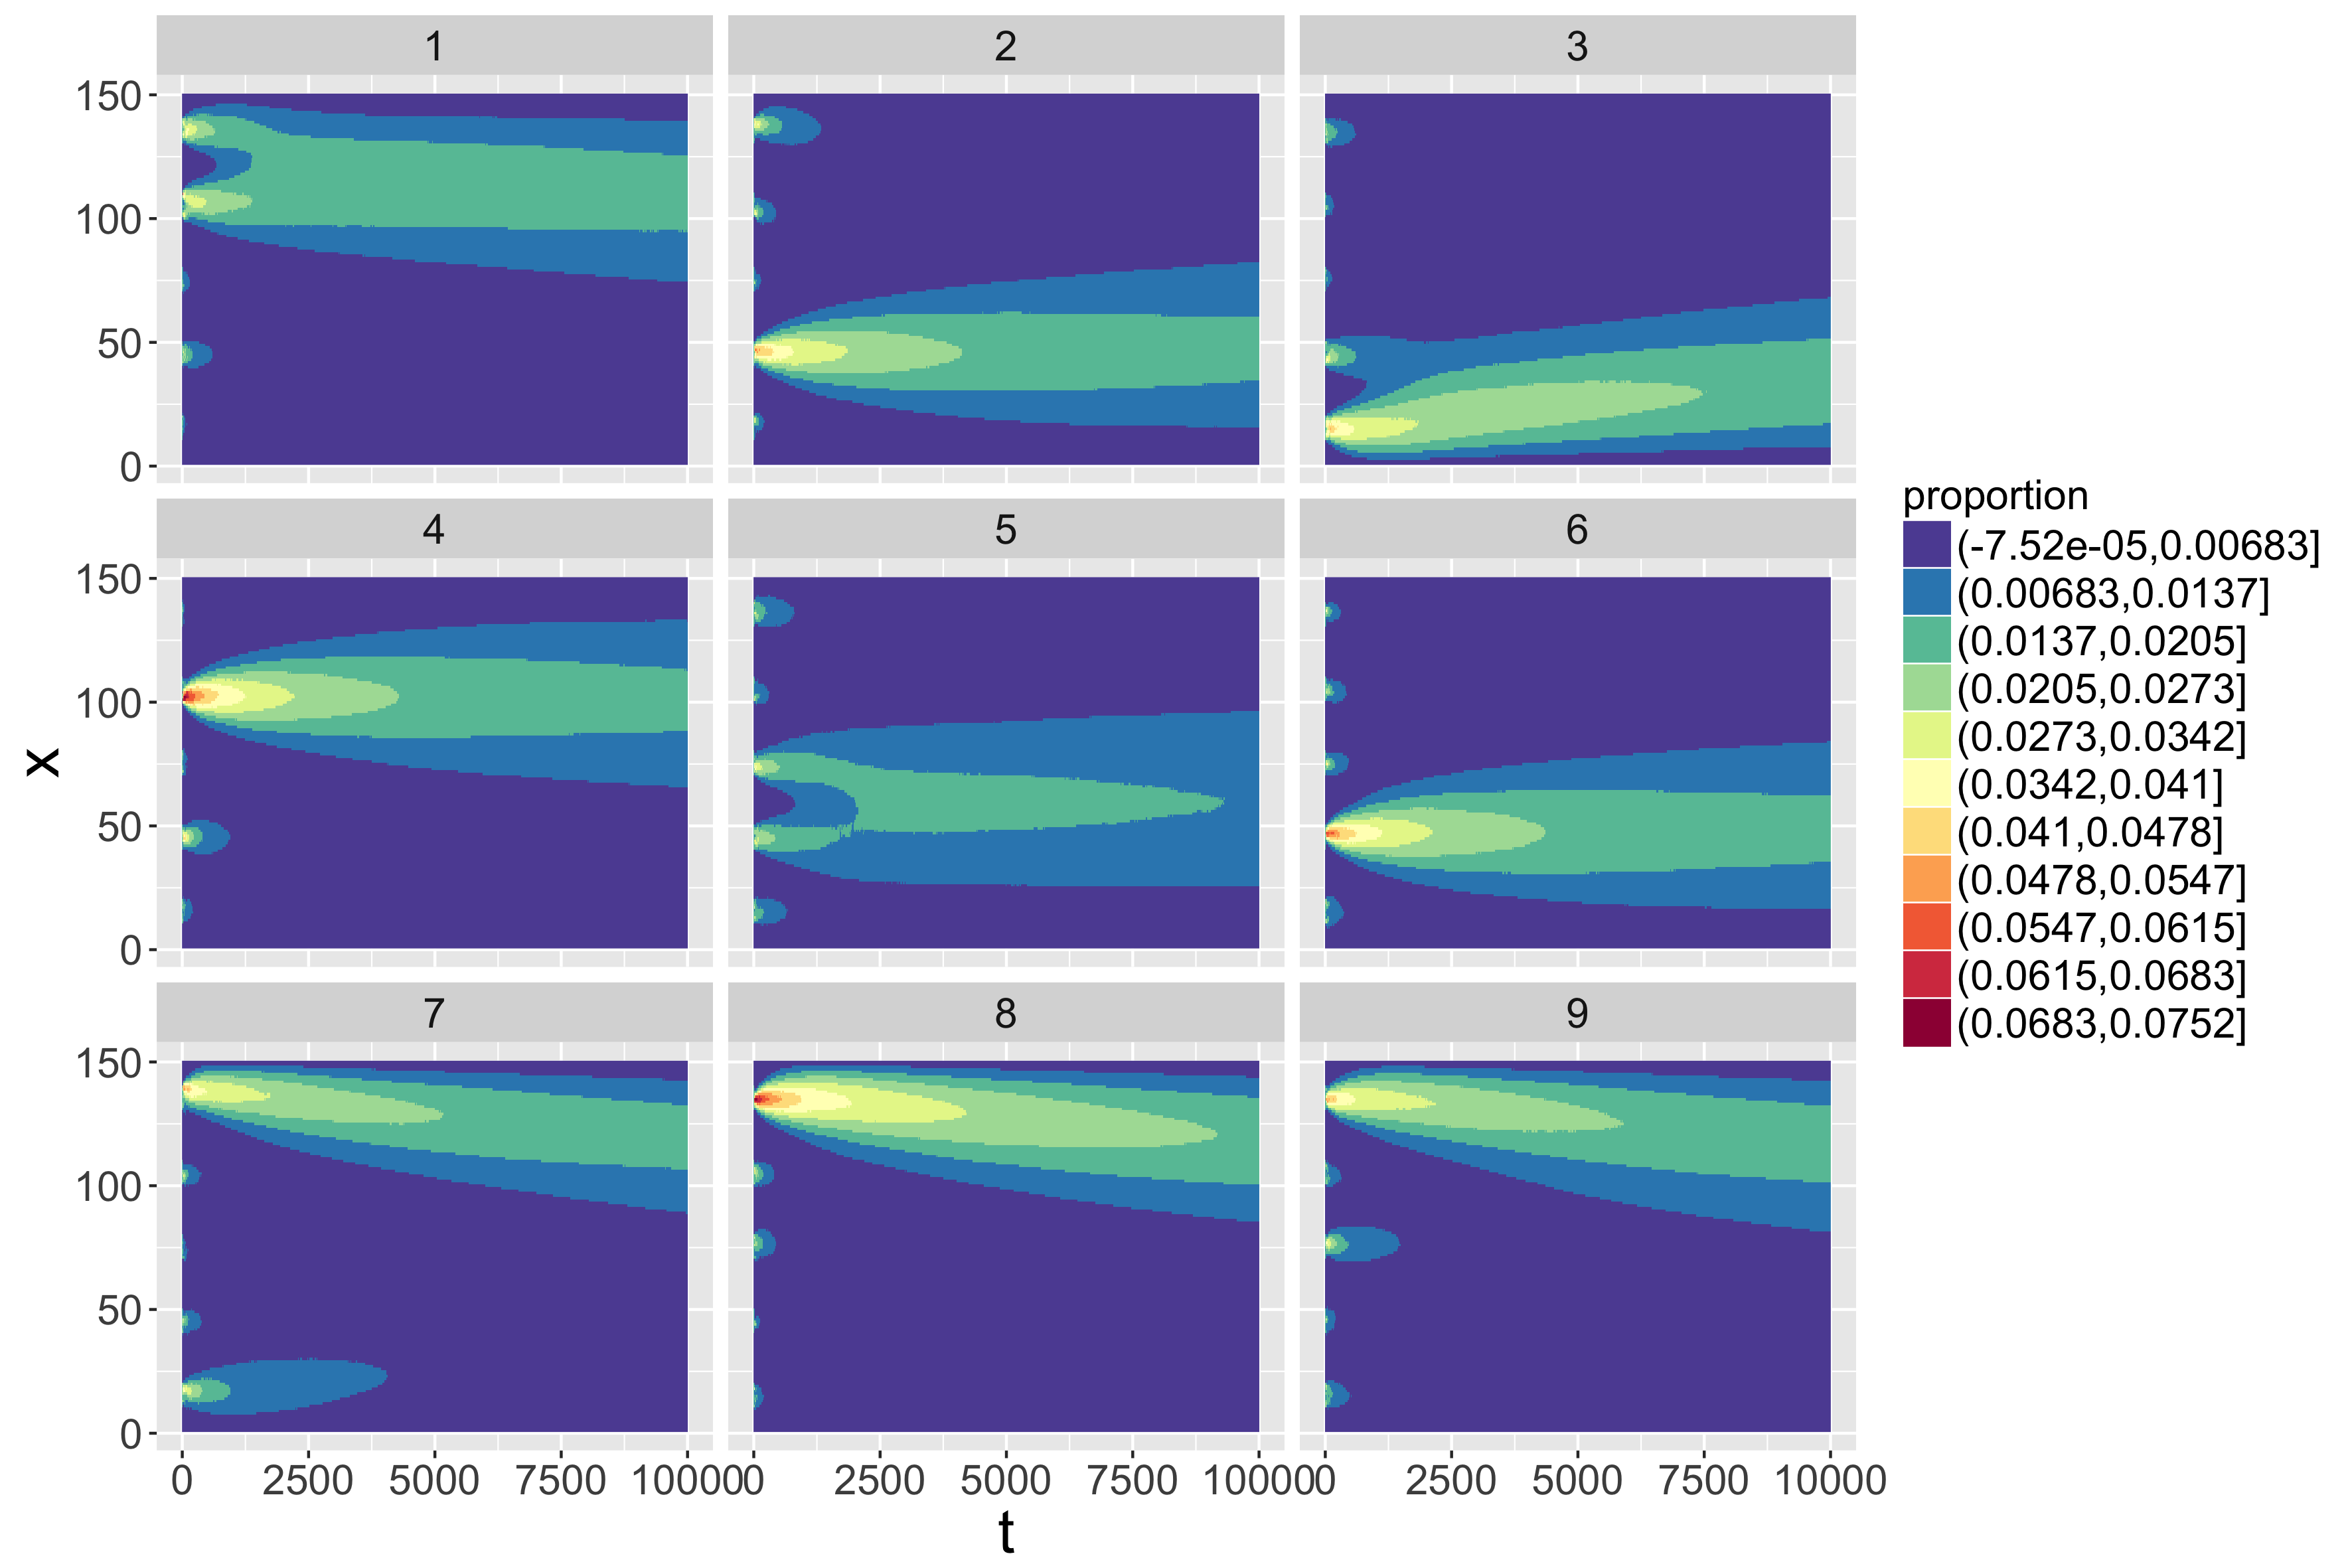
\includegraphics[width=\linewidth]{Figures/Density/Fig4.png}
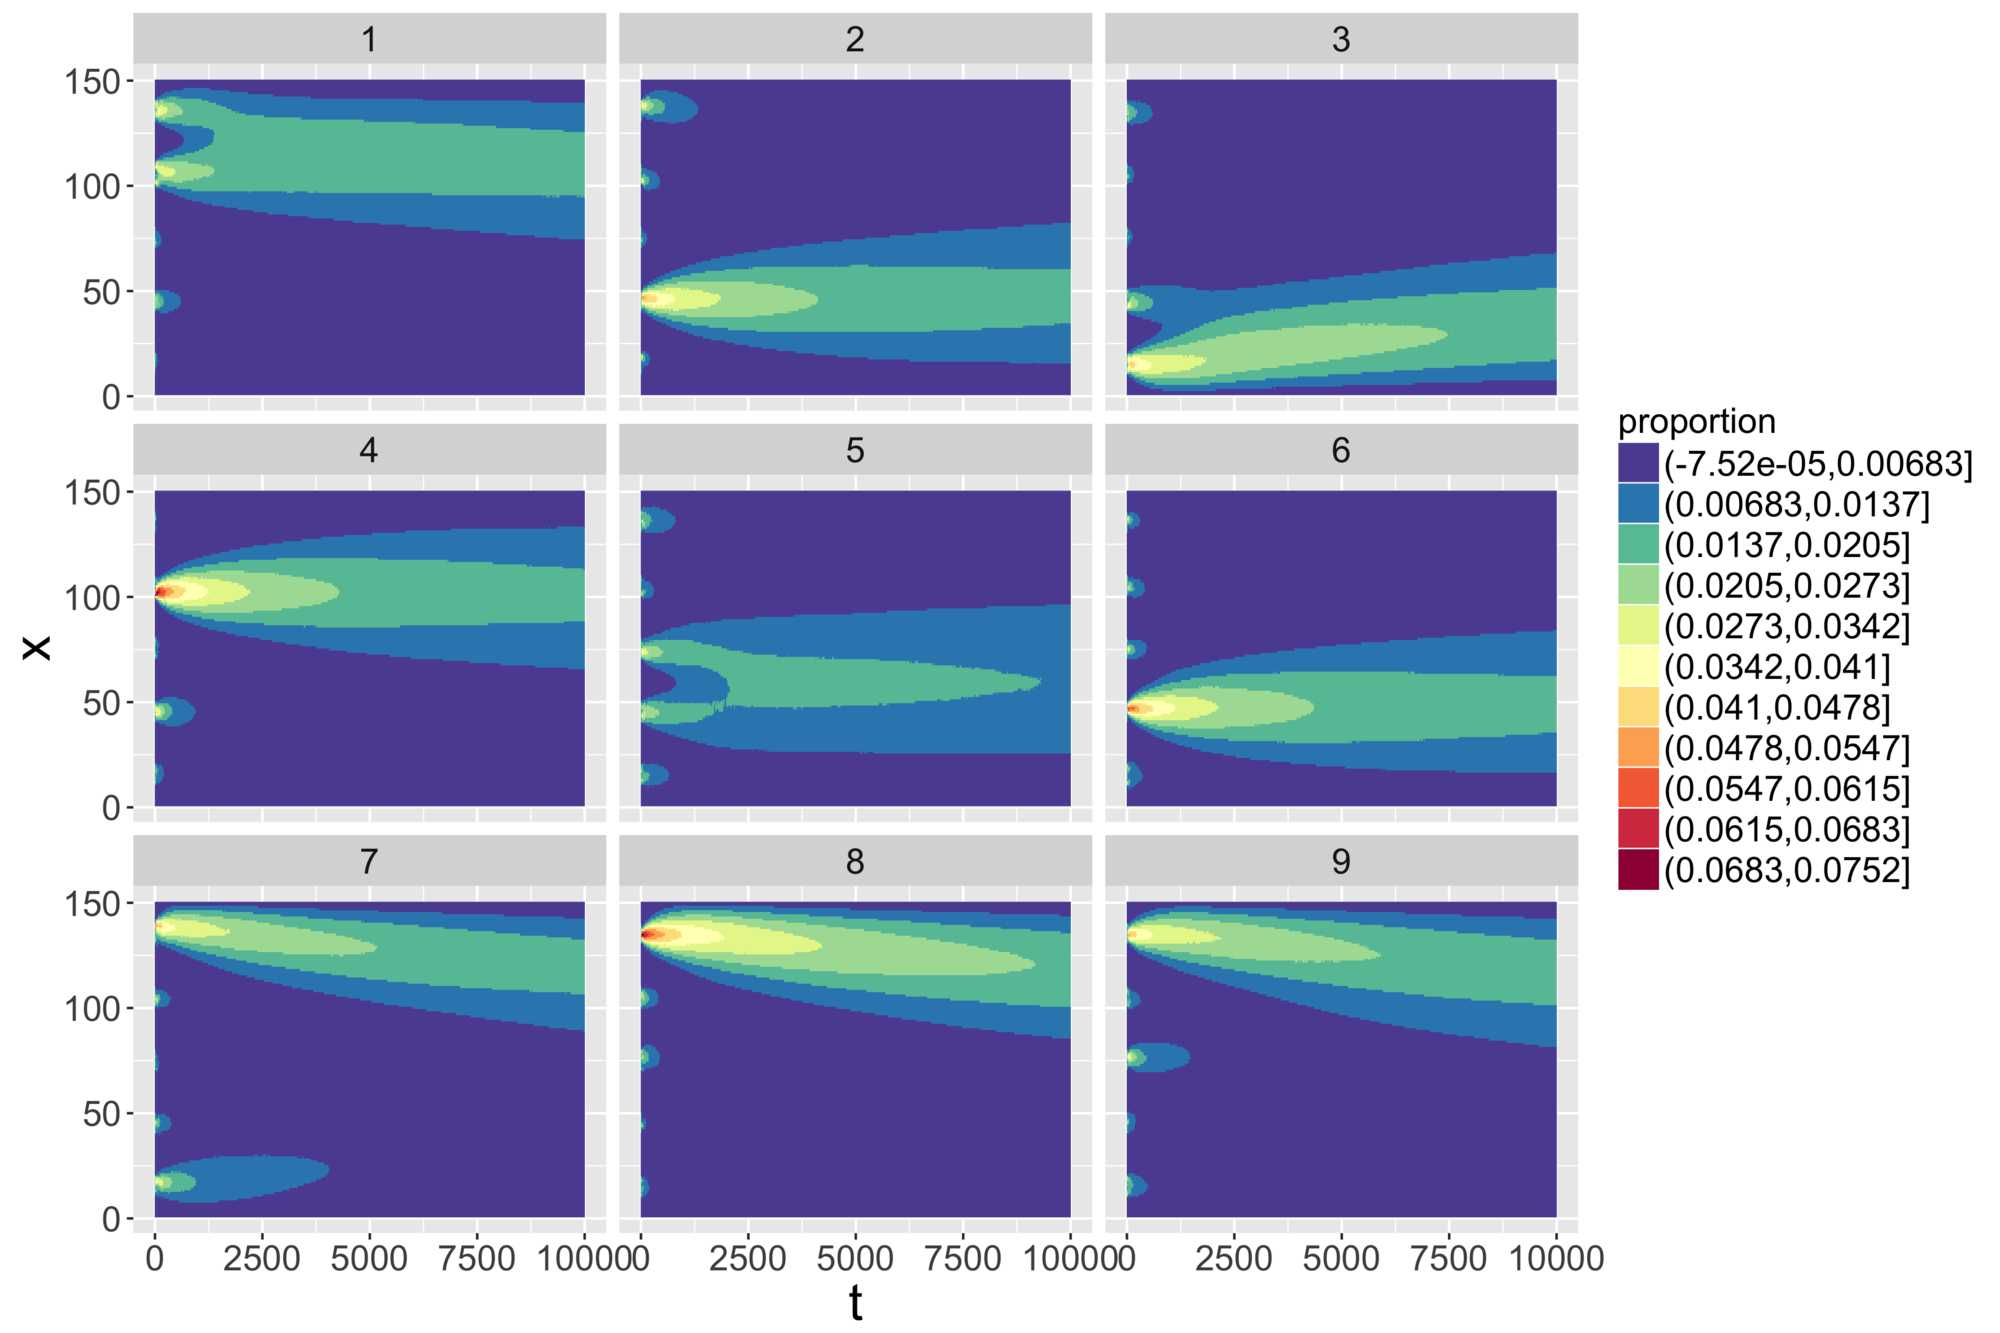
\includegraphics[width=\linewidth]{Figures/Final/5-2-2-fig-density-fig4}
\caption[Randomness and frozen accidents][Dépendance au chemin]{\textbf{Randomness and frozen accidents.} We show nine random realizations of the one dimensional system with similar initial conditions, namely five equidistant equally populated initial cells. Parameters are $\alpha = 1.4,\beta =0.1,N_G=10$. Each plot shows time against space, color level giving the proportion of population in each cell.\label{fig:density:fig4}}{\textbf{Aléatoire et accidents figés.} Nous montrons 9 réalisations aléatoires du système à une dimension avec des conditions initiales identiques, c'est à dire 5 cellules équidistantes peuplées également à l'instant initial. Les paramètres sont $\alpha = 1.4,\beta =0.1,N_G=10$. Chaque graphe montre le temps contre l'espace, le niveau de couleur donnant la proportion de population dans chaque cellule.\label{fig:density:fig4}}
\end{figure}
%%%%%%%%%%%%%





%%%%%%%%%%%%%%%%%%%%%%%%
\subsubsection{Model Calibration}{Calibration du modèle}


\bpar{
We finally turn to the the calibration of the model, that is done on the morphological objectives. As a single calibration for each real cell is computationally out of reach, we use the previous model exploration and superpose the point clouds with real indicator values. Full scatterplots of all indicators against each other, for simulated and real configurations, are given in~\ref{app:sec:density}. We find that the real point cloud is mostly contained within the simulated, that extend in significantly larger areas. It means that for a large majority of real configuration, there exist model parameters producing in average exactly the same morphological configuration. The highest discrepancy is for the distance indicator, the model failing to reproduce configuration with high distance, low Moran and intermediate hierarchy. These could for example correspond to polycentric configurations with many consequent centers. We consider a more loose calibration constraint, by doing a Principal Component Analysis on synthetic and real morphological values, and consider the two first components only. These represent 85\% of cumulated variance. The rotated point clouds along these dimensions are shown in Fig.~\ref{fig:density:densitycalib}. Most of real point cloud falls in the simulated one in this simplified setting. We illustrate particular points with real configurations and their simulated counterparts: for example Bucharest, Romania, corresponds to a monocentric semi-stationary configuration, with very high aggregation but also diffusion and a rather low growth rate. Other examples show less populated areas in Spain and Finland. From the plots giving parameter influence, we can show that most real situation fall in the region with intermediate $\alpha$ but quite varying $\beta$. It is consistent with real scaling urban exponents having a variation range rather small (between 0.8 and 1.3 generally~\cite{pumain2006evolutionary}) compared to the one we allowed in the simulations, whereas the diffusion processes may be much more diverse. This way, we have shown that the model is able to reproduce most of existing urban density configuration in Europe, despite its rather simplicity. It confirms that in terms of urban form, most of drivers at this scale can be translated into these abstract processes of aggregation and diffusion, but also that function must be quite correlated with form since the dimension of function (with an additional economic dimension in form for example) is not taken into account in the model.
}{
Nous traitons finalement la calibration du modèle, qui est faite sur les objectifs morphologiques. Comme une calibration pour chaque cellule réelle est hors de portée en terme de calcul, nous utilisons l'exploration précédente du modèle et superposons le nuage de points avec les valeurs réelles des indicateurs. Les scatterplots complets de chaque indicateur contre les autres, pour les configurations simulées et les réelles, sont donnés en~\ref{app:sec:density}. Nous constatons que le nuage de points réels est en majorité contenu dans le simulé, qui s'étend sur des zones significativement plus grandes. Cela signifie que pour une grande majorité des configurations réelles, il existe des valeurs des paramètres qui produisent en moyenne exactement la même configuration morphologique. Les plus grands écarts est pour l'indicateur de distance, le modèle échouant à produire des configurations avec une valeur élevée de la distance, un Moran faible et une hiérarchie intermédiaire. Cela peut par exemple correspondre à des configurations polycentriques avec de nombreux centres conséquents. Nous considérons une contrainte de calibration plus faible, en procédant à une analyse en composantes principales sur les valeurs normalisées des indicateurs morphologiques pour les configurations synthétiques et réelles, et ne considérons que les deux premières composantes seulement. Celles-ci représentent 85\% de la variance cumulée. Les nuages de points projeté sur ces dimensions est montré en Fig.~\ref{fig:density:densitycalib}. La majorité du nuage réel tombe dans le simulé dans cette configuration simplifiée. Nous illustrons des points particuliers avec des configurations réelles et leur contrepartie simulée: par exemple Bucarest, Roumanie, correspond à une configuration monocentrique semi-stationnaire, avec une forte agrégation mais aussi diffusion et un taux de croissance plutôt bas. Les autres exemples montrent des zones moins peuplées en Espagne et en Finlande. A partir des graphes montrant l'influence des paramètres, on peut montrer que la plupart des situations réelles tombent dans la région avec des valeurs intermédiaires pour $\alpha$ mais $\beta$ assez variable. Cela est cohérent avec le fait que les exposants de lois d'échelles urbaines ont une plage de variation plutôt étroite (entre 0.8 et 1.3 généralement~\cite{pumain2006evolutionary}) comparée à celle que nous avons permis dans les simulations, tandis que les processus de diffusion peuvent être bien plus divers. Ainsi, nous avons montré que le modèle est capable de reproduire la majorité des configuration de densité en Europe, malgré sa relative simplicité. Cela confirme qu'en terme de forme urbaine, la plupart des facteurs à cette échelle peuvent être traduits dans ces processus abstraits d'agrégation et de diffusion, mais aussi que la fonction doit être relativement corrélée à la forme puisque la dimension fonctionnelle (avec une dimension économique supplémentaire dans la forme par exemple) n'est pas prise en compte dans le modèle.
}


% Calib 1 :
% real : PC1 = 0.9544645 ; PC2 = 0.3296364 ; coordinates : -2.607152,39.74274 - Spain, Castilla-La Mancha, Cuenca ; synth : PC1 = 0.9487267 PC2 = 0.3245882 ; beta=0.108 ; NG=637 ; nd=1 ; alpha=1.14 ; population=13235.648362769914
% Calib 2 :
% real : PC1 = 0.7004772 ; PC2 = 0.2195029 ; coordinates : 27.16068,65.889 - Finland, Lapland;  synth :  PC1 = 0.6870686 ; PC2 = 0.2287785 ; beta=0.0060 ; NG=25 ; nd=1 ; alpha=0.4 ; population=849.895449367323
% Calib 3 :
% real : PC1 = 1.017064 ; PC2 = 0.3510089 ; coordinates : -2.561874,41.30203 - Spain, Castilla et Leon, Soria ; synth : PC1 = 1.005976 PC2 = 0.3950987 ; beta=0.166; NG=100;nd=1;alpha=1;population=10017.238452906771
% Calib 4 :
% real : PC1 = -0.00177 ; PC2 = 0.6006739 ; coordinates : 25.7361,44.69989 - Romania, Bucharest ; synth : PC1 = -0.0543461 PC2 = 0.5798307 ; beta=0.432;NG=1273;nd=4;alpha=3.87;population=63024.359885979036


%%%%%%%%%%%%%%%
\begin{figure}
%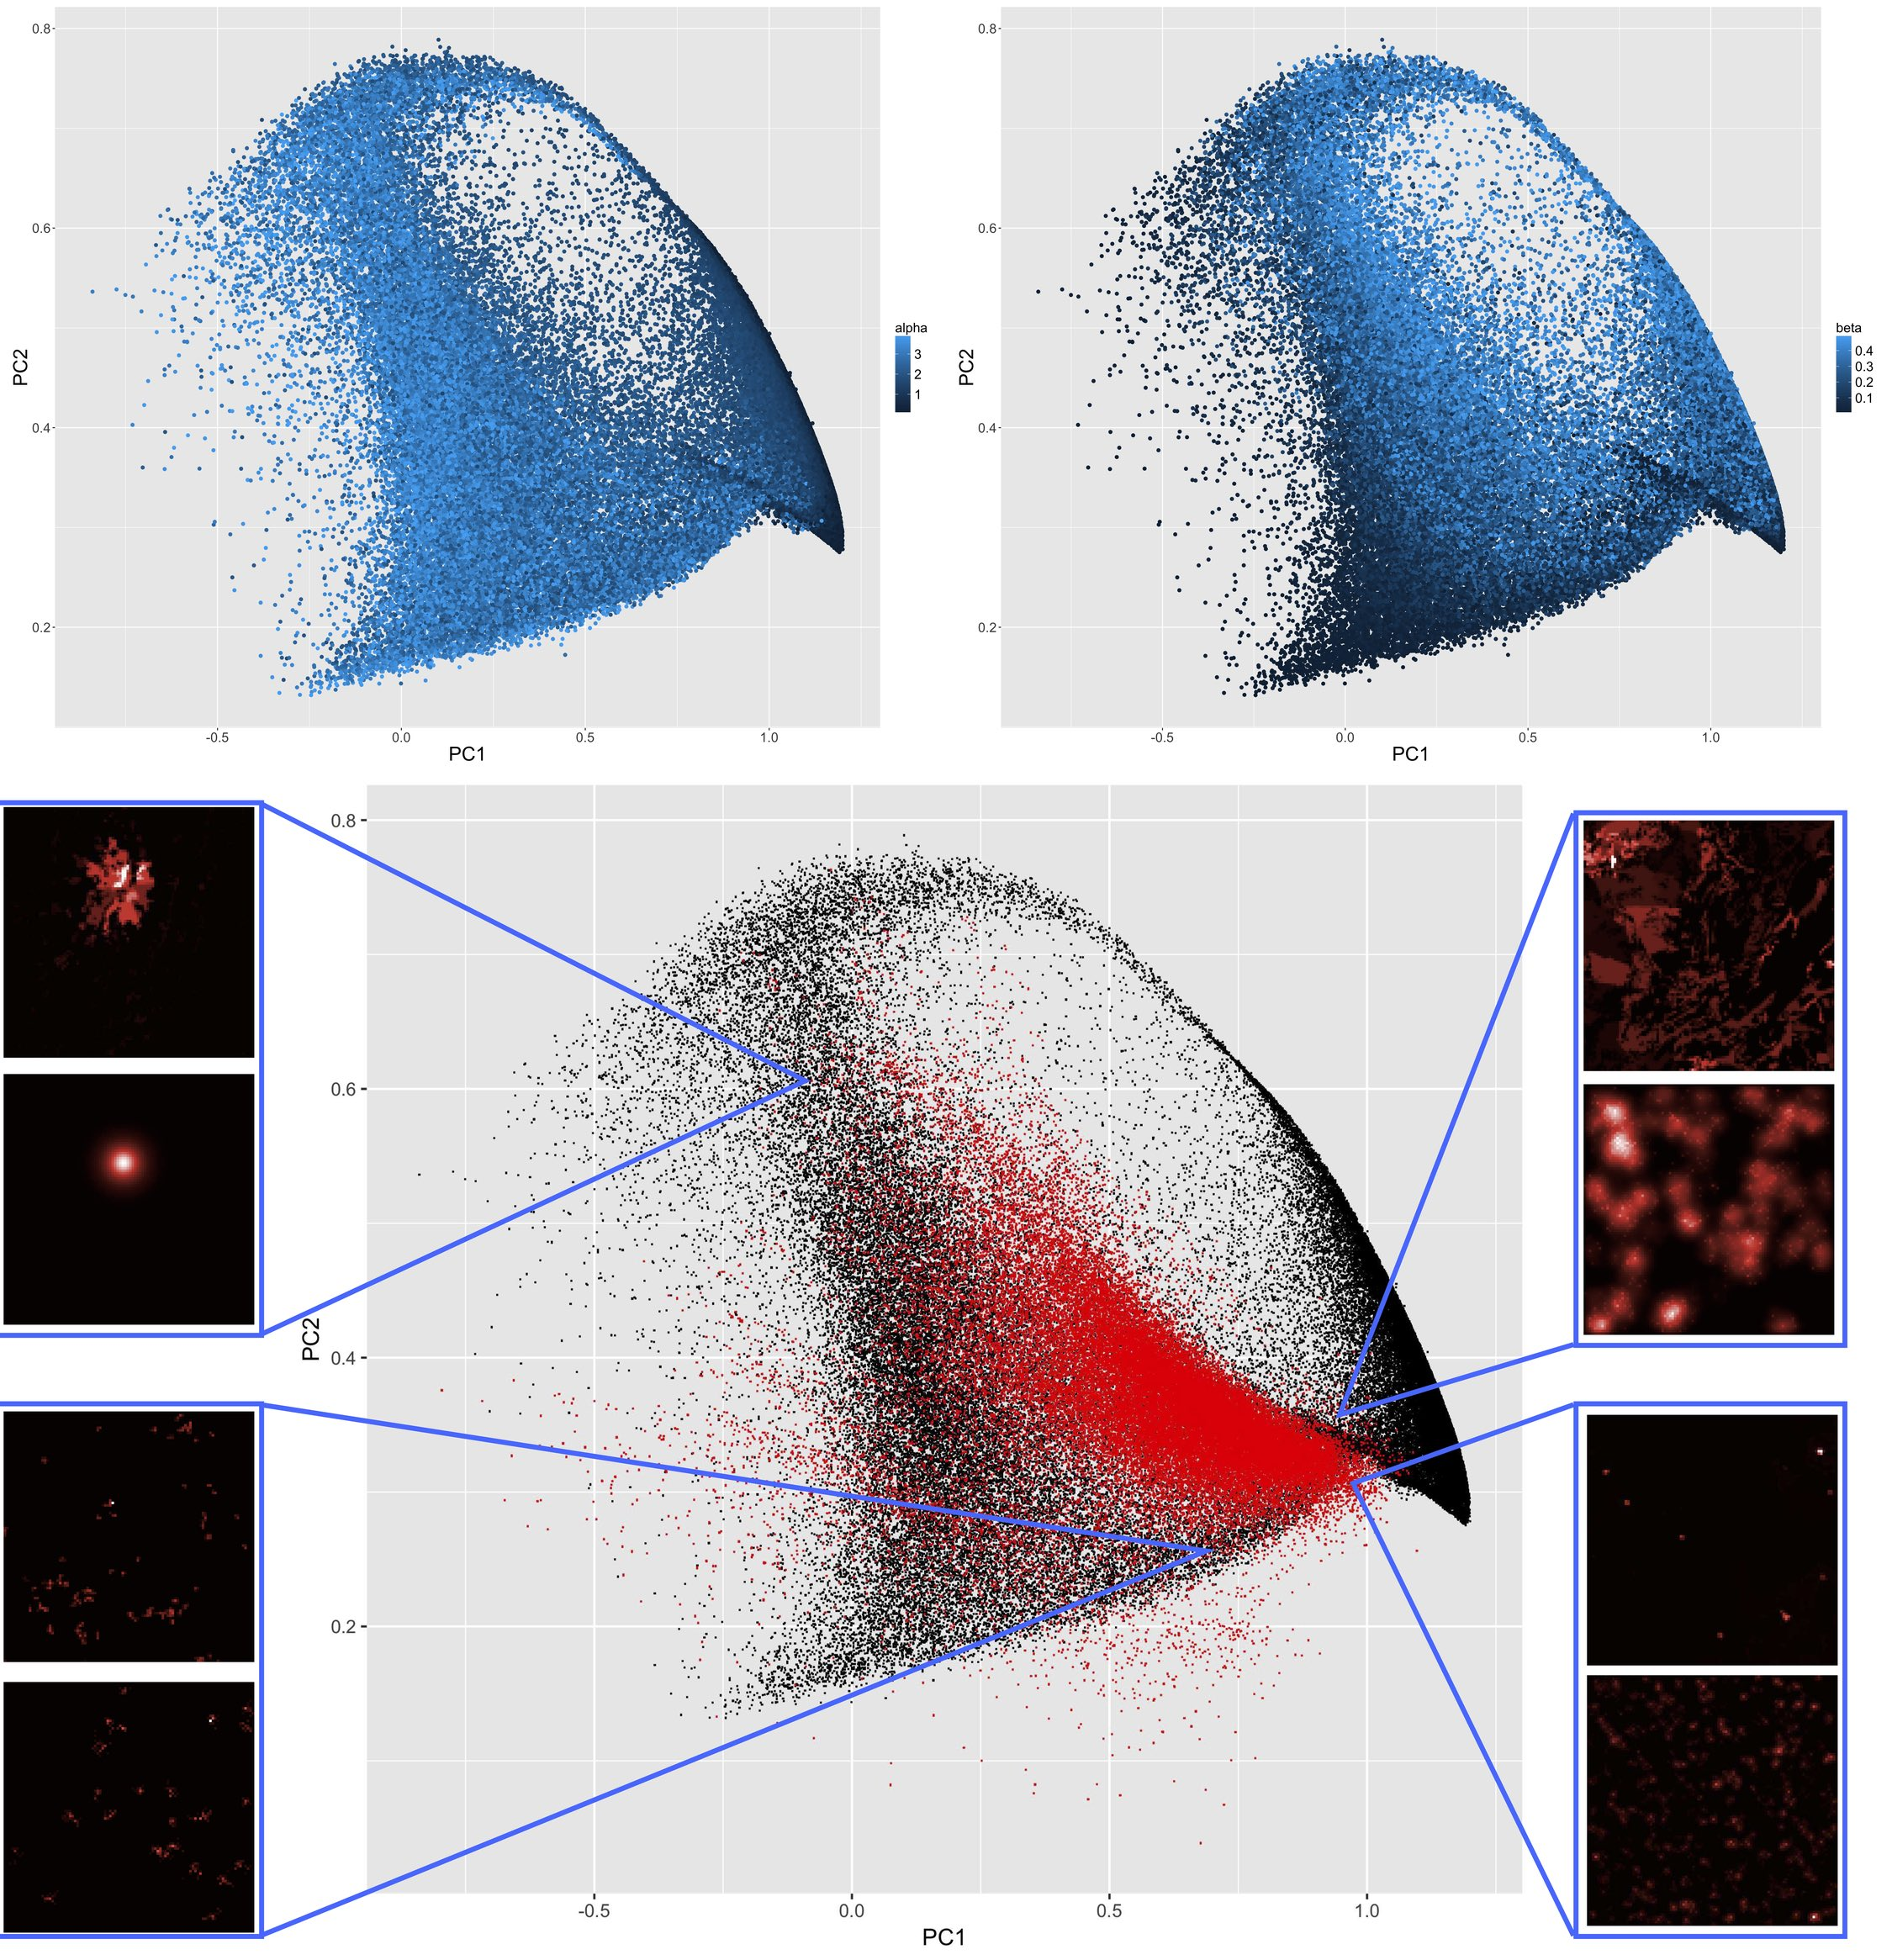
\includegraphics[width=\linewidth]{Figures/Density/Fig5}
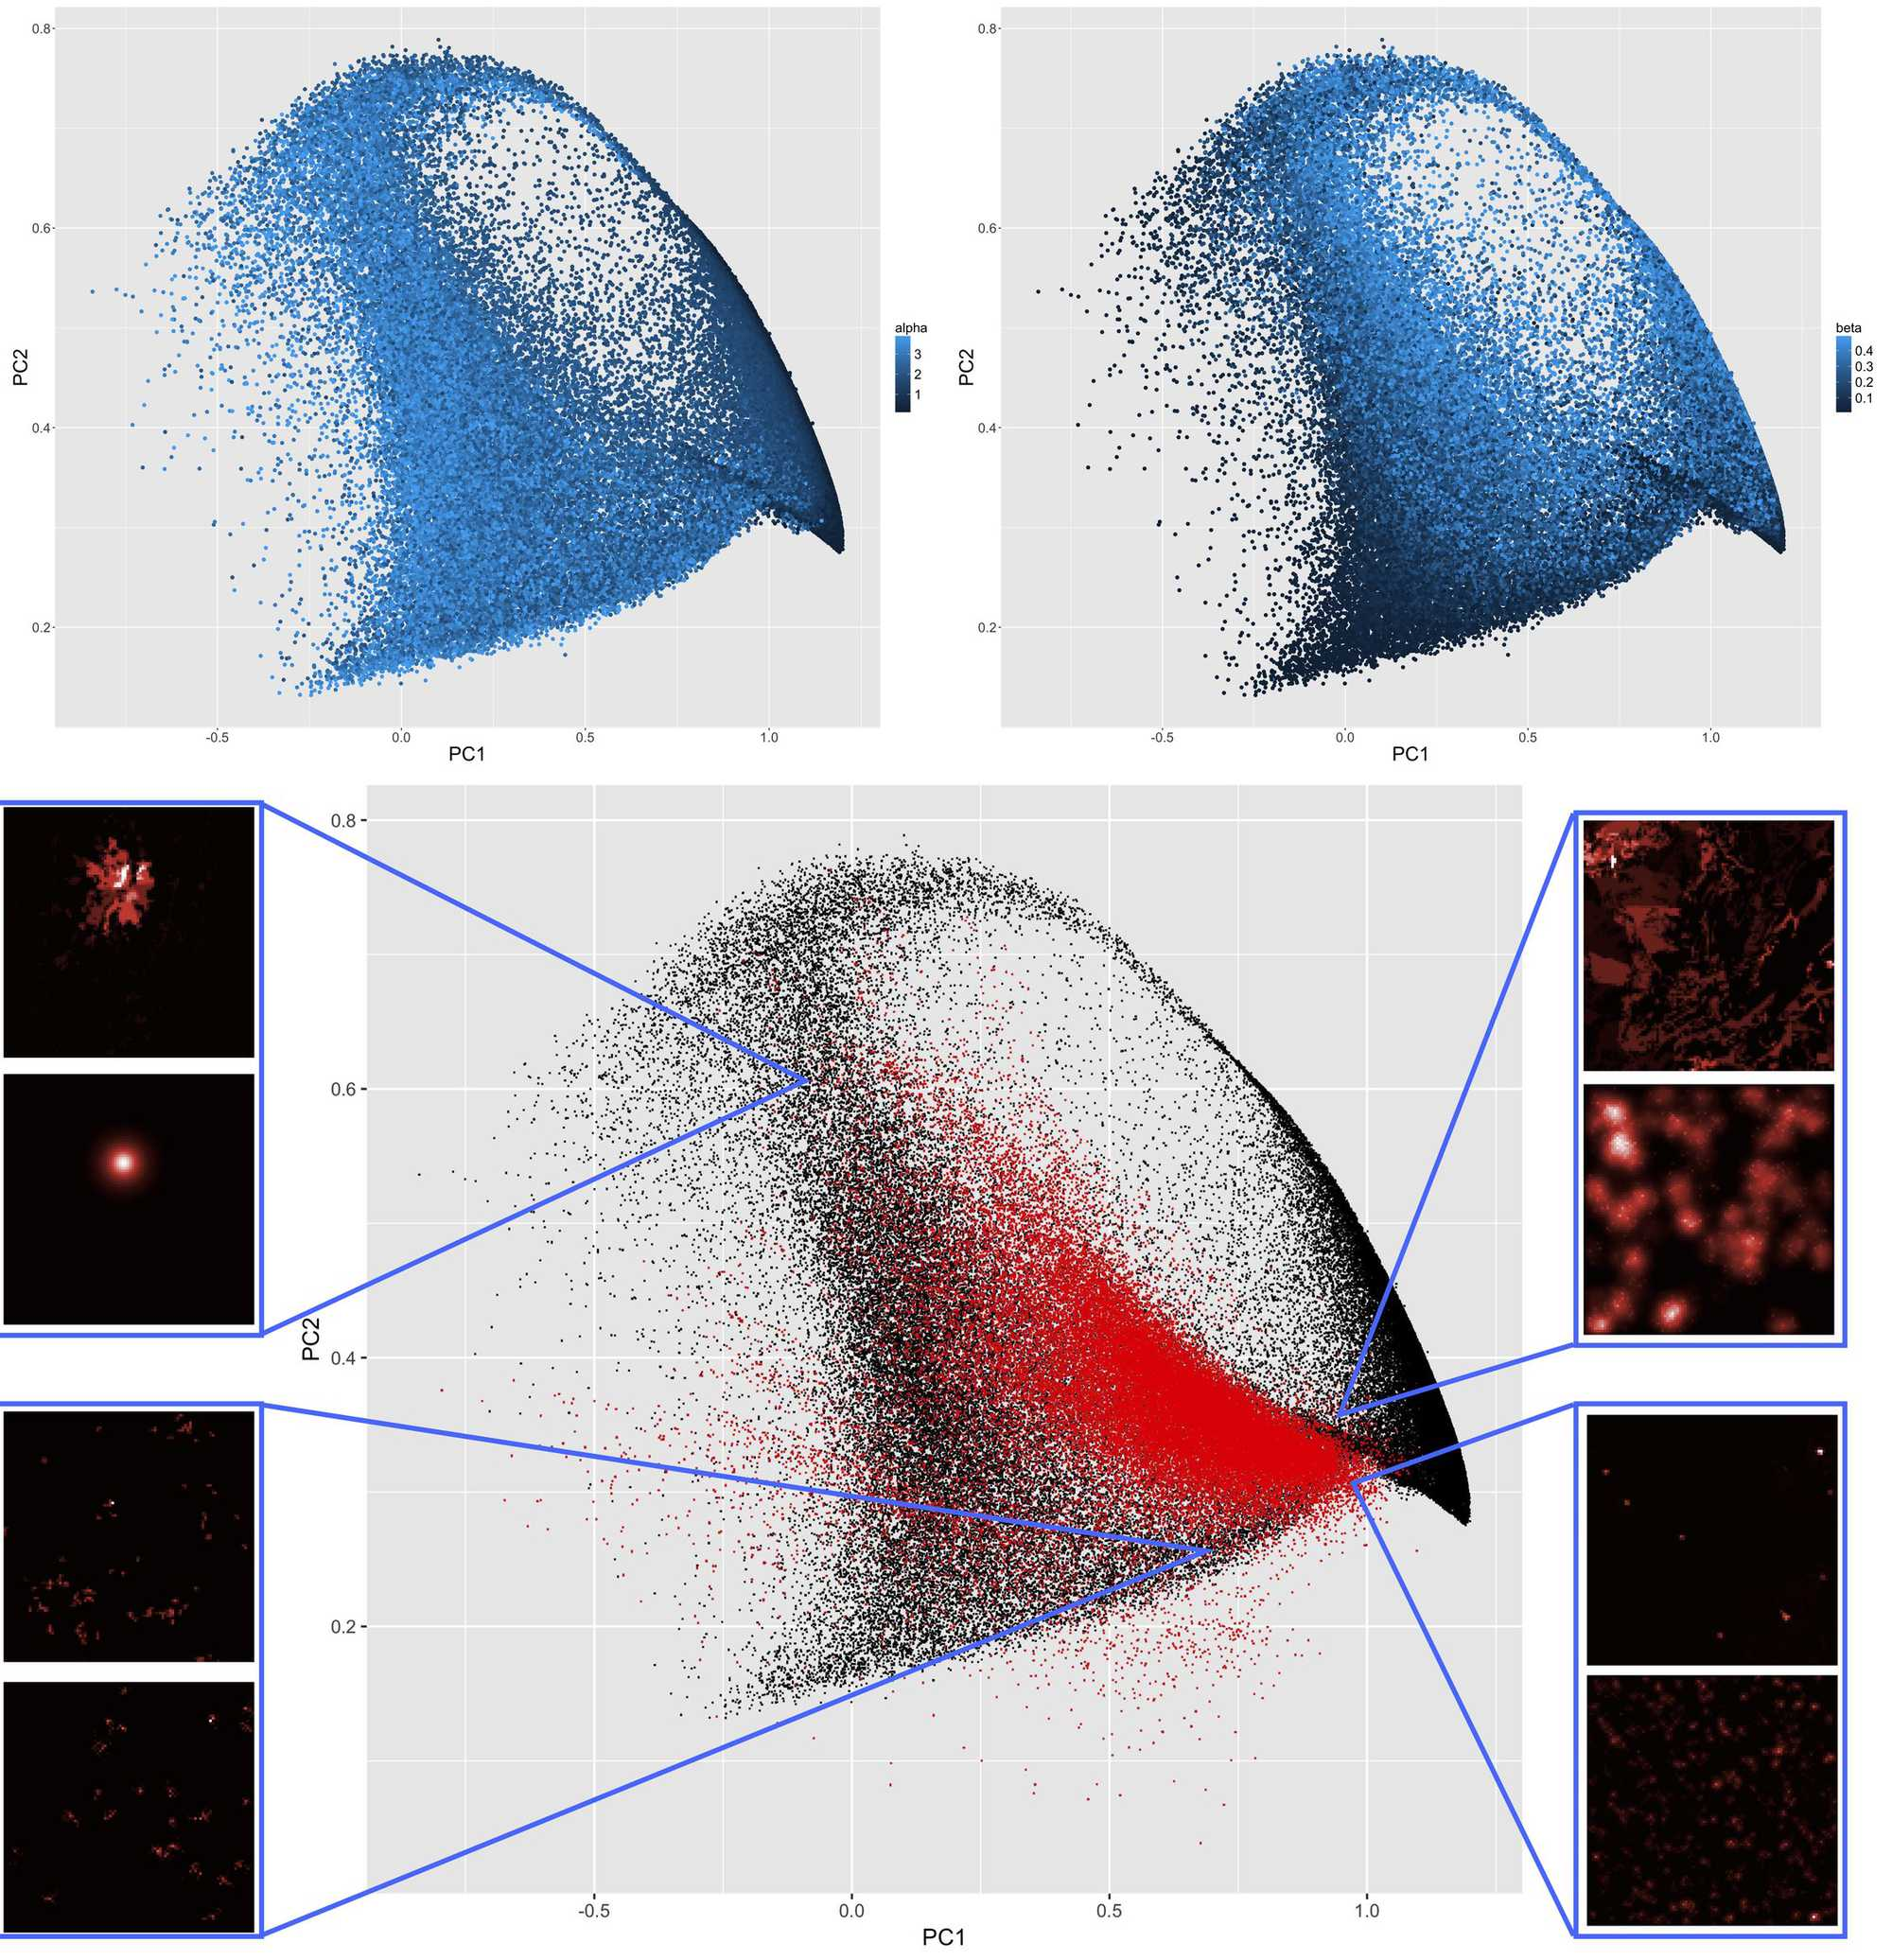
\includegraphics[width=\linewidth]{Figures/Final/5-2-2-fig-density-fig5}
\caption[Model calibration][Calibration du modèle]{\textbf{Model calibration.} \textit{(Top)} Simulated configurations in the two first principal components plan, color level giving the influence of $\alpha$ (left) and of $\beta$ (right); \textit{(Bottom)} Simulated points in the same space (in black) with real configurations (in red). We show around the plot typical examples of real configurations and their simulated counterparts in different regions of the space, the first being the real and the second the simulated in each case: Top left geographical coordinates 25.7361,44.69989 - Romania, Bucharest - simulation parameters $\alpha=3.87,\beta=0.432,N_G=1273,nd=4,P_m=63024$ ; Top right geographical coordinates -2.561874,41.30203 - Spain, Castilla et Leon, Soria - simulation parameters $\alpha=1,\beta=0.166,N_G=100,nd=1,P_m=10017$; Bottom left geographical coordinates 27.16068,65.889 - Finland, Lapland - simulation parameters $\alpha=0.4,\beta=0.006,N_G=25,nd=1,P_m=849$; Bottom right geographical coordinates -2.607152,39.74274 - Spain, Castilla-La Mancha, Cuenca - simulation parameters $\alpha=1.14,\beta=0.108,N_G=637,nd=1,P_m=13235$.\label{fig:densitycalib}}{\textbf{Calibration du modèle.} \textit{(Haut)} Configurations simulées dans le plan des deux premières composantes principales, le niveau de couleur donnant l'influence de $\alpha$ (gauche) et de $\beta$ (droite); \textit{(Bas)} Points simulés dans le même espace (en noir) avec les configurations réelles (en rouge). Autour du graphe sont montrés des exemples typiques de configurations réelles et leur contrepartie simulée dans différentes régions de l'espace, le premier étant le réel et le second le simulé dans chaque cas: haut gauche coordonnées 25.7361,44.69989 - Romania, Bucharest - paramètres $\alpha=3.87,\beta=0.432,N_G=1273,nd=4,P_m=63024$ ; Haut droite coordonnées -2.561874,41.30203 - Spain, Castilla et Leon, Soria - paramètres $\alpha=1,\beta=0.166,N_G=100,nd=1,P_m=10017$; Bas gauche coordonnées 27.16068,65.889 - Finland, Lapland - paramètres $\alpha=0.4,\beta=0.006,N_G=25,nd=1,P_m=849$; Bas droite coordonnées -2.607152,39.74274 - Spain, Castilla-La Mancha, Cuenca - paramètres $\alpha=1.14,\beta=0.108,N_G=637,nd=1,P_m=13235$.\label{fig:densitycalib}}
\end{figure}
%%%%%%%%%%%%%%








%%%%%%%%%%%%%%
\subsection{Discussion}{Discussion}




\paragraph{Calibration and model refinement}{Raffinement de la calibration et du modèle}


\bpar{
Further work on this simple model may consist in extracting the exact parameter space covering all real situations and provide interpretation of its shape, in particular through correlations between parameters and expressions of boundaries functions. Its volume in different directions should furthermore give the relative importance of parameters. Concerning the feasible space for the model of simulation itself, we tested a targeted exploration algorithm, giving promising results. More precisely, the Parameter Space Exploration (PSE) algorithm~\cite{10.1371/journal.pone.0138212} which is implemented in OpenMole, is aimed at determining all the possible outputs of a simulation model, i.e. samples its output space rather than input space. We obtain promising results as shown in Fig.~\ref{fig:fig6}: we find that the lower bound in Moran-entropy plan, confirmed by the algorithm, unexpectedly exhibit a scaling relationship. It would mean that at a given level of auto-correlation, that one could want to attain for sustainability reasons for example (optimality through co-location), imposes a minimal disorder in the configuration of activities. Other relations between indicators and as a function of parameters can be the object of similar future developments. The question of doing a dynamical calibration of the model, i.e. trying to reproduce configurations at successive times, is conditioned to the availability of population data at this resolution in time.
}{
Des développements futurs sur ce modèle simple peuvent consister à l'extraction de l'espace des paramètres exact couvrant l'ensemble des situations réelles et fournir une interprétation de sa forme, en particulier par les corrélations entre les paramètres et les expressions des fonctions de bordure. Son volume dans différentes directions devrait de plus donner l'importance relative des paramètres. Concernant l'espace faisable pour le modèle de simulation en lui-même, nous avons testé un algorithme d'exploration ciblée, qui donne des résultats prometteurs. Plus précisément, l'algorithme PSE~\cite{10.1371/journal.pone.0138212} qui est implémenté dans OpenMole, a pour but de déterminer toutes les sorties possibles d'un modèle de simulation, c'est à dire échantillonne son espace de sortie plutôt que d'entrée. Nous obtenons des résultats intéressants comme montré en Fig.~\ref{fig:density:fig6}: nous trouvons que la borne inférieure dans le plan Moran-entropie, confirmée par l'algorithme, exhibe une loi d'échelle de manière inattendue (puisqu'il est impossible a priori de déterminer cet espace non-faisable avec seule les formules des d'indicateurs, celui-ci étant témoin de la réalité de structures urbaines même simulées). Cela voudrait dire qu'à un niveau fixé d'auto-corrélation, qu'on pourrait vouloir atteindre pour des raisons de soutenabilité par exemple (optimalité par co-localisation), impose un désordre minimal dans la configuration des activités. D'autres relations entre indicateurs et comme fonction des paramètres peut être l'objet de développements futurs similaires. La possibilité d'une calibration dynamique du modèle, i.e. essayer de reproduire des configurations à des dates successives, est conditionnée à la disponibilité des données de population à cette résolution dans le temps.
}

% application of Calibration Profile algo to check relative influence of parameters ? out of context not interesting

%%%%%%%%%%%%%
\begin{figure}
%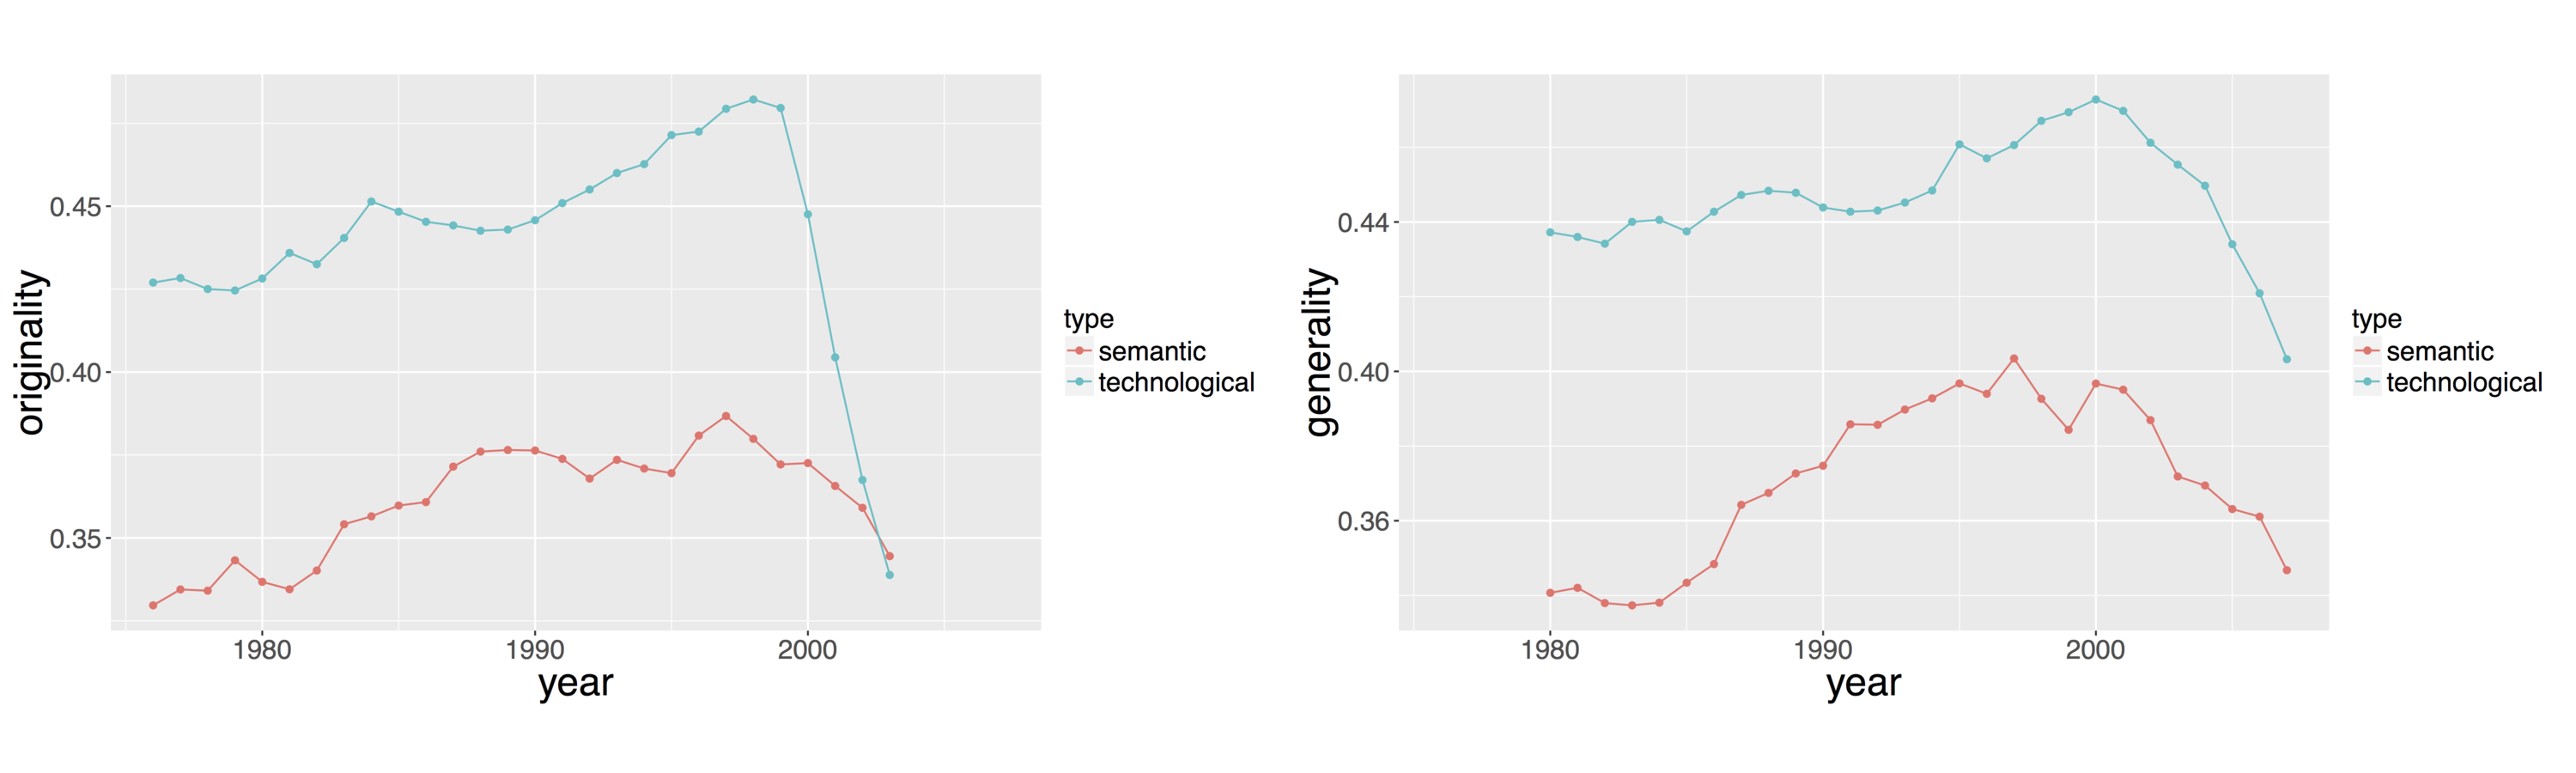
\includegraphics[width=\linewidth]{Figures/Density/Fig6.png}
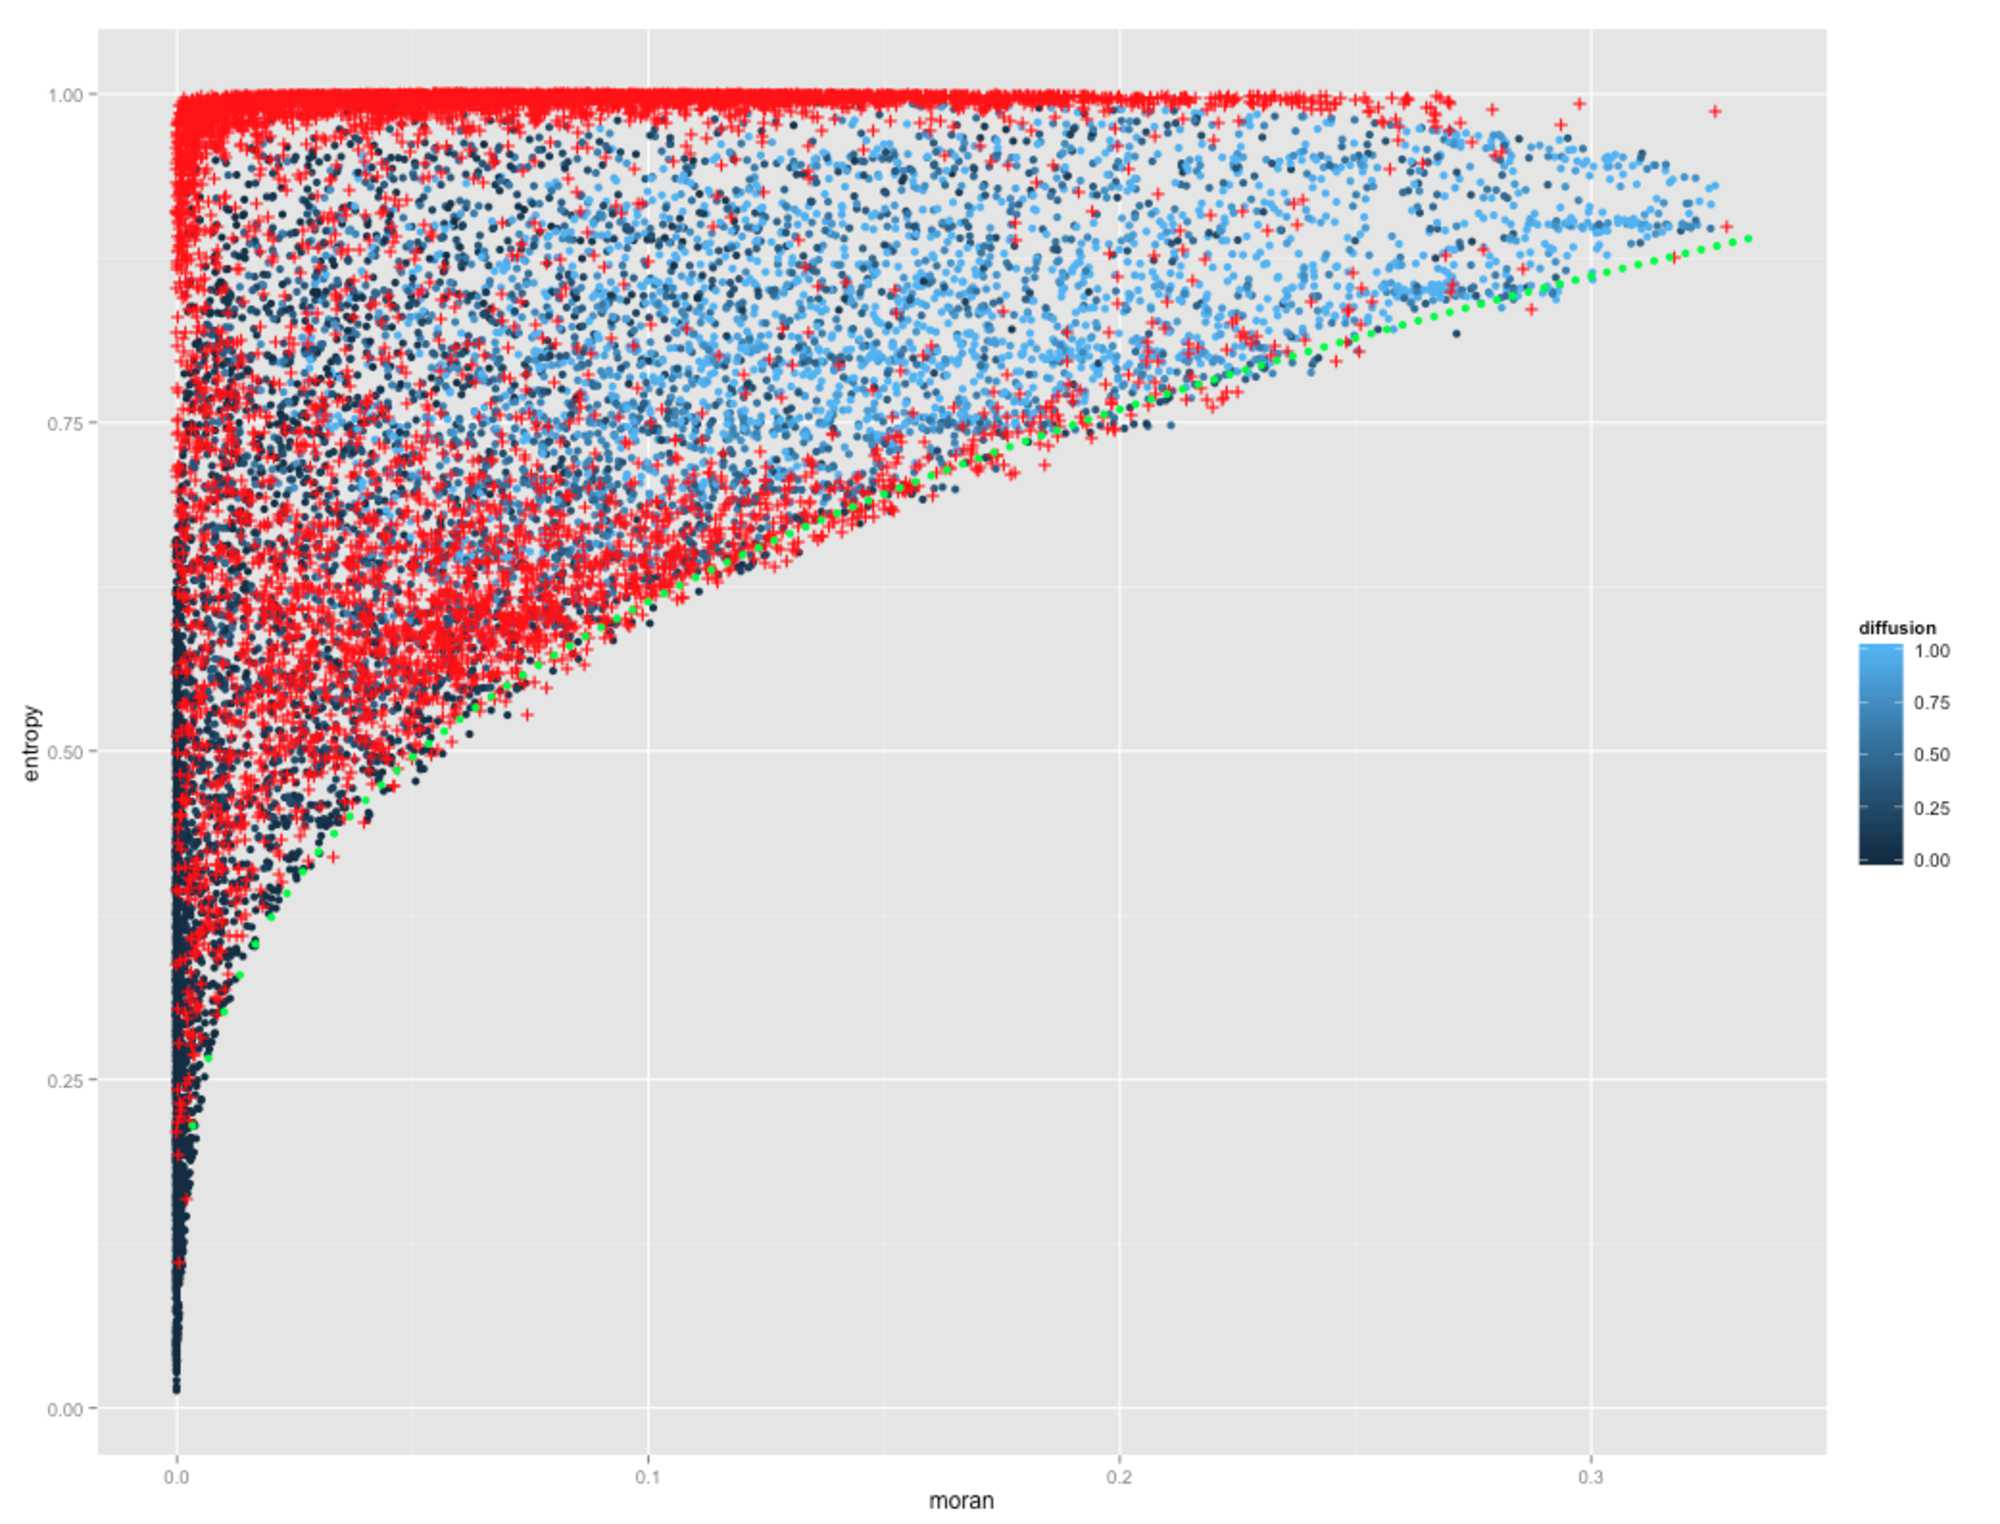
\includegraphics[width=\linewidth]{Figures/Final/5-2-2-fig-density-fig6}
\caption[PSE exploration][Exploration par PSE]{\textbf{PSE exploration.} Scatterplot of Moran against Entropy, with blue points obtained with LHS and red with PSE exploration. Green dashed line gives feasible lower bound.\label{fig:density:fig6}}{\textbf{Exploration par PSE.} Scatterplot de l'entropie en fonction de Moran, les points bleus étant obtenus par LHS et les rouges par PSE. La ligne pointillée verte donne la borne inférieur faisable.\label{fig:density:fig6}}
\end{figure}
%%%%%%%%%%%%%


\bpar{
We aimed at using abstract processes rather than having a highly realistic model. Tuning some mechanisms is possible to have a model closer to reality in microscopic processes: for example thresholding the local population density, or stopping the diffusion at a given distance from the center if it is well defined. It is however far from clear if these would produce such a variety of forms and could be calibrated in a similar way, as being accurate locally does not mean being accurate at the mesoscopic level for morphological indicators. Allowing the parameters to locally vary, i.e. being non stationary in space, or adding randomness to the diffusion process, are also potential model refinements.
}{
Nous avons visé à utiliser des processus abstraits plutôt que d'avoir un modèle hautement réaliste. La modification de certains mécanismes est possible pour avoir un modèle plus proche de la réalité des processus microscopiques: par exemple plafonner la densité de population locale, ou stopper la diffusion à une distance donnée du centre s'il est bien défini. Il est cependant loin d'être clair si ceux-ci produiraient une telle variété de formes et pourraient être calibrés de la même façon, puisqu'être précis localement n'implique pas d'être précis au niveau mesoscopique pour les indicateurs morphologiques. Permettre aux paramètres de varier localement, i.e. être non-stationnaires dans l'espace, ou ajouter de l'aléatoire au processus de diffusion, sont également des raffinements potentiels du modèle.
}


\paragraph{Integration into a multi-scale growth model}{Intégration dans un modèle de croissance multi-scalaire}

\bpar{
The question of the generic character of the model is also open: would it work as well when trying to reproduce Urban Forms on very different systems such as the United States or China. A first interesting development would be to test it on these systems and at slightly different scales (1km cell for example). Finally, we believe that a significant insight into the non-stationarity of Urban Systems would be allowed by its integration into a multi-scale growth model. Urban growth patterns have been empirically shown to exhibit multi-scale behavior~\cite{zhang2013identifying}. Here at the meso-scale, total population and growth rates are fixed by exogenous conditions of processes occurring at the macro-scale. It is particularly the aim of spatial growth models such as the Favaro-pumain model~\cite{favaro2011gibrat} to determine such parameters through relations between cities as agents. One would condition the morphological development in each area to the values of the parameters determined at the level above. In that setting, one must be careful of the role of the bottom-up feedback: would the emerging urban form influence the macroscopic behavior in its turn ? Such multi-scale complex model are promising but must be considered carefully.
}{
La question du caractère générique du modèle est également ouverte, c'est à dire s'il fonctionnerait de la même manière pour reproduire des formes urbaines sur des systèmes très différents comme les Etats-Unis ou la Chine. Un premier développement intéressant serait de le tester sur ces systèmes et à des échelles légèrement différentes (cellules de taille 1km par exemple). Enfin, nous pensons qu'un gain de connaissance important concernant la non-stationnarité des systèmes urbains serait rendu possible par son intégration dans un modèle de croissance multi-échelles. Les motifs de croissance urbaine ont été prouvés empiriquement exhibant un comportement multi-échelle~\cite{zhang2013identifying}. Ici à l'échelle mesoscopique, la population totale et le taux de croissance sont fixés par les conditions exogènes de processus se produisant à l'échelle macroscopique. C'est particulièrement le but des modèles spatiaux de croissance comme le modèle Favaro-Pumain~\cite{favaro2011gibrat} de déterminer de tels paramètres par les relations entre villes comme agents. On pourrait conditionner le développement morphologique de chaque zone aux valeurs des paramètres déterminés au niveau supérieur. Dans ce contexte, il faudrait être prudent sur le rôle de la retroaction bottom-up: la forme urbaine émergente devrait-elle influence le comportement macroscopique à son tour ? De tels modèles complexes multi-scalaires sont prometteurs mais doivent être considérés avec précaution.
}


%  determination of effective independent dimensions of the urban system at this scale ?


\bpar{
In conclusion, we have provided a calibrated spatial urban morphogenesis model at the mesoscopic scale that can reproduce any European urban pattern in terms of morphology. We demonstrate that the abstract processes of aggregation and diffusion are sufficient to capture urban growth processes at this scale. It is meaningful in terms of policies based on urban form such as energy efficiency, but also means that issues out of this scope must be tackled at other scales or through other dimensions of urban systems.
}{
En conclusion, nous avons produit un modèle spatial de morphogenèse urbaine à l'échelle mesoscopique, dont la calibration permet de reproduire n'importe quelle configuration urbaine Européenne en terme de morphologie. Nous démontrons que les processus abstraits d'agrégation et diffusion sont suffisants pour capturer la dimension morphologique des processus de croissance urbaine à cette échelle. Cela a des implications par exemple en terme de politiques basées sur la forme urbaine comme l'efficacité énergétique, mais aussi signifie que les questions hors de ce cadre doivent être traitées à d'autres échelles ou par d'autres dimensions des systèmes urbains.
}





\stars
















%----------------------------------------------------------------------------------------


\newpage


\section{Correlated generation of territorial configurations}{Génération de configurations territoriales corrélées}



This section aims to explore the sequential coupling between previous model of density generation and an heuristic of network growth. We explore therein the feasible space of correlations between network measures and morphological measures.% This work was initially presented as a methodological investigation in 


%%%%%%%%%%%%%%%%%%%%%%
\subsection{Correlated geographical data of density and network}{Données Géographiques corrélées de Densité et de Réseau}


%%%%%%%%%%%%%%%%%%%%%%
\subsubsection{Context}{Contexte}



\bpar{
The use of synthetic data in geography is generally directed towards the generation of synthetic populations within agent-based models (mobility, \emph{LUTI} models)~\cite{pritchard2009advances}. We can make a weak link with some Spatial Analysis techniques. The extrapolation of a continuous spatial field from a discrete spatial sample through a kernel density estimation for example can be understood as the creation of a synthetic dataset (even if it is not generally the initial view, as in Geographically Weighted Regression~\cite{brunsdon1998geographically} in which variable size kernels do not interpolate data \emph{stricto sensu} but extrapolate abstract variables representing interaction between explicit variables). In the field of modeling in quantitative geography, \emph{toy-models} or hybrid models require a consistent initial spatial configuration. A set of possible initial configurations becomes a synthetic dataset on which the model is tested. The first Simpop model~\cite{sanders1997simpop}, precursor of a large family of models later parametrized with real data, could enter that frame but was studied on an unique synthetic spatialization. Similarly underlined was the difficulty to generate an initial transportation infrastructure in the case of the SimpopNet model~\cite{schmitt2014modelisation} although it was admitted as a cornerstone of knowledge on the behavior of the model. A systematic control of spatial configuration effects on the behavior of simulation models was only recently proposed~\cite{cottineau2015revisiting}, approach that can be interpreted as a statistical control on spatial data. The aim is to be able to distinguish proper effects due to intrinsic model dynamics from particular effects due to the geographical structure of the case study. Such results are essential for the validation of conclusions obtained with modeling and simulation practices in quantitative geography.
}{
En géographie, l'utilisation de données synthétiques est plus généralement axée vers l'utilisation de population synthétiques au sein de modèles basés agents (mobilité, modèles \emph{LUTI})~\cite{pritchard2009advances}. On peut également citer des méthodes d'analyse spatiales qui s'en rapprochent : par exemple, l'extrapolation d'un champ spatial continu à partir d'un échantillon discret, par une estimation par noyaux par exemple, peut être compris comme la génération d'un jeu de données synthétiques (même si ce n'est pas le point de vue initial, comme pour la Regression Géographique Pondérée~\cite{brunsdon1998geographically}, dans laquelle les noyaux de taille variables n'interpolent pas des données au sens propre mais extrapolent des variables abstraites représentant l'interaction entre variables explicites). Dans le domaine de la modélisation en géographie quantitative, dans le cas de \emph{modèles jouets} ou de modèles hybrides, une configuration initiale cohérente est souvent essentielle : un ensemble de configurations initiales possibles est alors un jeu de données synthétiques sur lesquelles le modèle est testé : le premier modèle Simpop~\cite{sanders1997simpop}, pionnier d'une famille de modèles par la suite paramétrisés par des données réelles, pourrait rentrer dans ce cadre mais était lancé sur une spatialisation synthétique unique. De même, il a été souligné la difficulté de générer une configuration initiale pour une infrastructure de transport dans le cas du modèle SimpopNet~\cite{schmitt2014modelisation}, alors qu'il s'agit un point essentiel dans la connaissance du comportement du modèle. Il a récemment été proposé de contrôler systématiquement les effets de la configuration spatiale sur le comportement de modèles de simulation spatialisés~\cite{cottineau2015revisiting}, méthodologie pouvant être interprétée comme un contrôle par données statistiques spatiales. L'enjeu est de pouvoir alors distinguer effets propres dus à la dynamique intrinsèque du modèle, d'effet particuliers dus à la structure géographique du cas d'application. Celui-ci est crucial pour la validation des conclusions issues des pratiques de modélisation et simulation en géographie quantitative.
}



%%%%%%%%%%%%%%%%%%%%%%
\subsubsection{Formalization}{Formalisation}


\bpar{
We propose in our case to generate territorial systems summarized in a simplified way as a spatial population density $d(\vec{x})$ and a transportation network $n(\vec{x})$. Correlations we aim to control are correlations between urban morphological measures and network measures. The question of interactions between territories and networks is already well-studied~\cite{offner1996reseaux} but stays highly complex and difficult to quantify~\cite{offner1993effets}. A dynamical modeling of implied processes should shed light on these interactions (\cite{bretagnolle:tel-00459720}, p. 162-163). We develop in that frame a \emph{simple} coupling (i.e. without any feedback loop) between a density distribution model and a network morphogenesis model.
}{
Dans notre cas, nous proposons de générer des systèmes de villes représentés par une densité spatiale de population $d(\vec{x})$ et la donnée d'un réseau de transport $n(\vec{x})$, représenté de façon simplifiée, pour lesquels on serait capable de contrôler les correlations entre mesures morphologiques de la densité urbaine et caractéristiques du réseau. La question de l'interaction entre territoire et réseaux de transport est un sujet d'étude classique~\cite{offner1996reseaux} mais extrêmement complexe et difficile à quantifier~\cite{offner1993effets}. Une modélisation dynamique des processus impliqués devrait apporter des connaissances sur ces interactions (\cite{bretagnolle:tel-00459720}, p. 162-163). Dans ce cadre, nous développons un couplage \emph{simple} (c'est à dire sans boucle de rétroaction) entre un modèle de morphogenèse urbaine et un modèle de génération de réseau.
}


\paragraph{Density model}{Modèle de densité}


\bpar{
The density model is the model described and explored in the previous section. We use it for the conditional generation of network.
}{
Les modèle de densité est celui décrit et exploré dans la section précédente. Nous l'utilisons pour la génération conditionnelle du réseau.
}

\paragraph{Network model}{Modèle de réseau}


\bpar{
On the other hand, we are able to generate a planar transportation network by a model $N$, at a similar scale and given a density distribution. Because of the conditional nature to the density of the generation process, we will first have conditional estimators for network indicators, and secondly natural correlations between network and urban shapes should appear as processes are not independent. The nature and modularity of these correlations as a function of model parameters are still to determine by exploration of the coupled model.
}{
D'autre part, on est capable de générer par un modèle $N$ un réseau de transport planaire à une échelle équivalente, étant donné une distribution de densité. La génération du réseau étant conditionnée à la donnée de la densité, les estimateurs des indicateurs de réseau seront conditionnels d'une part, et d'autre part les formes urbaines et du réseau devraient nécessairement être corrélées, les processus n'étant pas indépendants. La nature et la modularité de ces correlations selon la variation des paramètres des modèles restent à déterminer par l'exploration du modèle couplé.
}



\bpar{
The heuristic network generation procedure is the following :
\begin{enumerate}
\item A fixed number $N_c$ of centers that will be first nodes of the network si distributed given density distribution, following a similar law to the aggregation process, i.e. the probability to be distributed in a given patch is $\frac{(P_i/P)^{\alpha}}{\sum (P_i/P)^{\alpha}}$. Population is then attributed according to Voronoi areas of centers, such that a center cumulates population of patches within its extent.
\item Centers are connected deterministically by percolation between closest clusters : as soon as network is not connected, two closest connected components in the sense of minimal distance between each vertices are connected by the link realizing this distance. It yields a tree-shaped network.
\item Network is modulated by potential breaking in order to be closer from real network shapes. More precisely, a generalized gravity potential between two centers $i$ and $j$ is defined by
\[
V_{ij}(d) = \left[ (1 - k_h) + k_h \cdot \left( \frac{P_i P_j}{P^2} \right)^{\gamma} \right]\cdot \exp{\left( -\frac{d}{r_g (1 + d/d_0)} \right)}
\]
where $d$ can be euclidian distance $d_{ij}=d(i,j)$ or network distance $d_N(i,j)$, $k_h \in [0,1]$ a weight to modulate role of populations, $\gamma$ giving shape of the hierarchy across population values, $r_g$ characteristic interaction distance and $d_0$ distance shape parameter.
\item A fixed number $K\cdot N_L$ of potential new links is taken among couples having greatest euclidian distance potential ($K=5$ is fixed).
\item Among potential links, $N_L$ are effectively realized, that are the one with smallest rate $\tilde{V}_{ij} = V_{ij}(d_N)/V_{ij}(d_{ij})$. At this stage only the gap between euclidian and network distance is taken into account : $\tilde{V}_{ij}$ does indeed not depend on populations and is increasing with $d_N$ at constant $d_{ij}$.
\item Planarity of the network is forced by creation of nodes at possible intersections created by new links.
\end{enumerate}
}{
La procédure de génération heuristique de réseau est la suivante :
\begin{enumerate}
\item Un nombre fixé $N_c$ de centres qui seront les premiers noeuds du réseau est distribué selon la distribution de densité, suivant une loi similaire à celle d'agrégation, i.e. la probabilité d'être distribué sur une case est $\frac{(P_i/P)^{\alpha}}{\sum (P_i/P)^{\alpha}}$. La population est ensuite répartie selon les zones de Voronoi des centres, un centre cumulant la population des cases dans son emprise.
\item Les centres sont connectés de façon déterministe par percolation entre plus proches clusters : tant que le réseau n'est pas connexe, les deux composantes connexes les plus proches au sens de la distance minimale entre chacun de leurs sommets sont connectées par le lien réalisant cette distance. On obtient alors un réseau arborescent.
\item Le réseau est alors modulé par ruptures de potentiels afin de se rapprocher de formes réelles. Plus précisément, un potentiel d'interaction gravitaire généralisé entre deux centres $i$ et $j$ est défini par
\[
V_{ij}(d) = \left[ (1 - k_h) + k_h \cdot \left( \frac{P_i P_j}{P^2} \right)^{\gamma} \right]\cdot \exp{\left( -\frac{d}{r_g (1 + d/d_0)} \right)}
\]

où $d$ peut être la distance euclidienne $d_{ij}=d(i,j)$ ou la distance par le réseau $d_N(i,j)$, $k_h \in [0,1]$ un poids permettant de changer le rôle des population dans le potentiel, $\gamma$ régissant la forme de la hiérarchie selon les valeurs des populations, $r_g$ distance caractéristique de décroissance et $d_0$ paramètre de forme.
\item Un nombre $K\cdot N_L$ de nouveaux liens potentiels est pris comme les couples ayant le plus grand potentiel pour la distance euclidienne ($K=5$ est fixé).
\item Parmi les liens potentiels, $N_L$ sont effectivement réalisés, qui sont ceux ayant le plus faible rapport $V_{ij}(d_N)/V_{ij}(d_{ij})$ : à cette étape seul l'écart entre distance euclidienne et distance par le réseau compte, ce rapport ne dépendant plus des populations et étant croissant en $d_N$ à $d_{ij}$ fixé.
\item Le réseau est planarisé par création de noeuds aux intersections éventuelles créées par les nouveaux liens.
\end{enumerate}
}



\bpar{
We insist on the fact that the network generation procedure is entirely heuristic and result of thematic assumptions (connected initial network, gravity-based link creation) combined with trial-and-error during first explorations. Other model types could be used as well, such biological self-generated networks~\cite{tero2010rules}, local network growth based on geometrical constraints optimization~\cite{barthelemy2008modeling}, or a more complex percolation model than the initial one that would allow the creation of loops for example. We could thus in the frame of a modular architecture, in which the choice between different implementations of a functional brick can be seen as a meta-parameter~\cite{cottineau2015incremental}, choose network generation function adapted to a specific need (as e.g. proximity to real data, constraints on output indicators, variety if generated forms, etc. ).
}{
Notons que la construction du modèle de génération est heuristique, et que d'autres types de modèles comme un réseau biologique auto-généré~\cite{TeroAl10}, une génération par optimisation locale de contraintes géométriques \cite{barthelemy2008modeling} ou un modèle de percolation plus complexe que celui utilisé, peuvent le remplacer. Ainsi, dans le cadre d'une architecture modulaire où le choix entre différentes implémentations d'une brique fonctionnelle peut être vue comme méta-paramètre~\cite{cottineau2015incremental}, on pourrait choisir la fonction de génération adaptée à un besoin donné (par exemple proximité à des données réelles, contraintes sur les relations entre indicateurs de sortie, variété de formes générées, etc.).
}



%  must do a computational benchmark for various network generation models ; calibrated on real data. -> cf network generation section.

\paragraph{Parameter space}{Espace des paramètres}


\bpar{
Parameter space for the coupled model\footnote{Weak coupling allows to limit the total number of parameters as a strong coupling would involve retroaction loops and consequently associated parameters to determine their structure and intensity. In order to diminish it, an integrated model would be preferable to a strong coupling, what is slightly different in the sense where it is not possible in the integrated model to freeze one of the subsystems to obtain a model of the other subsystem that would correspond to the non-coupled model.} is constituted by density generation parameters $\vec{\alpha}_D = (P_m/N_G , \alpha,\beta , n_d)$ (we study for the sake of simplicity the rate between population and growth rate instead of both varying, i.e. the number of steps needed to generate the distribution) and network generation parameters $\vec{\alpha}_N=(N_C,k_h,\gamma , r_g , d_0)$. We denote $\vec{\alpha} = (\vec{\alpha}_D,\vec{\alpha}_N)$. 
}{
L'espace des paramètres du modèle couplé\footnote{Le couplage faible permet de limiter le nombre total de paramètres puisqu'un couplage fort incluant des boucles de retroaction comprendrait nécessairement des paramètres supplémentaires pour régler la forme et l'intensité de celles-ci. Pour espérer le diminuer, il faudrait concevoir un modèle intégré, ce qui est différent d'un couplage fort dans le sens où il n'est pas possible de figer l'un des sous-systèmes pour obtenir un modèle de l'autre correspondant au modèle non-couplé.} est constitué des paramètres de génération de densité $\vec{\alpha}_D = (P_m/N_G , \alpha,\beta , n_d)$ (on s'intéresse pour simplifier au rapport entre population et taux de croissance, i.e. le nombre d'étapes nécessaires pour générer) et des paramètres de génération de réseau $\vec{\alpha}_N=(N_C,k_h,\gamma , r_g , d_0)$. On notera $\vec{\alpha} = (\vec{\alpha}_D,\vec{\alpha}_N)$.
}




% these notion of weak / strong coupling are not enough developed or reference-based. ---> find it in literature ? not sure exists like that. --> integarte it in theoretical paper ? or separate working paper.

\paragraph{Indicators}{Indicateurs}


\bpar{
Urban form and network structure are quantified by numerical indicators in order to modulate correlations between these. Morphology is defined as a vector $\vec{M}=(r,\bar{d},\varepsilon,a)$ giving spatial auto-correlation (Moran index), mean distance, entropy and hierarchy (see~\cite{le2015forme} for a precise definition of these indicators). Network measures $\vec{G} = (\bar{c},\bar{l},\bar{s},\delta)$ are with network denoted $(V,E)$
\begin{itemize}
\item Mean centrality $\bar{c}$ defined as average \emph{betweeness-centrality} (normalized in $[0,1]$) on all links.
\item Mean path length $\bar{l}$ given by $\frac{1}{d_m}\frac{2}{|V|\cdot (|V|-1)}\sum_{i<j}d_N(i,j)$ with $d_m$ normalization distance taken here as world diagonal $d_m=\sqrt{2}N$.
\item Mean network speed~\cite{banos2012towards} which corresponds to network performance compared to direct travel, defined as $\bar{s} = \frac{2}{|V|\cdot (|V|-1)}\sum_{i<j}{\frac{d_{ij}}{d_N(i,j)}}$.
\item Network diameter $\delta = \max_{ij}d_N(i,j)$.
\end{itemize}
}{
On quantifie la forme urbaine et la forme du réseau, dans le but de moduler la corrélation entre ces indicateurs. La forme est définie par un vecteur $\vec{M}=(r,\bar{d},\varepsilon,a)$ donnant auto-corrélation spatiale (indice de Moran), distance moyenne, entropie, hiérarchie (voir~\cite{le2015forme} pour une définition précise de ces indicateurs). Les mesures de la forme du réseau $\vec{G} = (\bar{c},\bar{l},\bar{s},\delta)$ sont, avec le réseau noté $(V,E)$,
\begin{itemize}
\item Centralité moyenne $\bar{c}$, définie comme la moyenne de la \emph{betweeness-centrality} (normalisée dans $[0,1]$) sur l'ensemble des liens.
\item Longueur moyenne des chemins $\bar{l}$ définie par $\frac{1}{d_m}\frac{2}{|V|\cdot (|V|-1)}\sum_{i<j}d_N(i,j)$ avec $d_m$ distance de normalisation prise ici comme la diagonale du monde $d_m=\sqrt{2}N$.
\item Vitesse moyenne~\cite{banos2012towards}, qui correspond à la performance du réseau par rapport au trajet à vol d'oiseau, définie par $\bar{s} = \frac{2}{|V|\cdot (|V|-1)}\sum_{i<j}{\frac{d_{ij}}{d_N(i,j)}}$.
\item Diamètre du réseau $\delta = \max_{ij}d_N(i,j)$
\end{itemize}
}



\paragraph{Covariance and correlation}{Covariance et COrrelation}


\bpar{
We study the cross-correlation matrix $\Covb{\vec{M}}{\vec{G}}$ between morphology and network. We estimate it on a set of $n$ realizations at fixed parameter values $(\vec{M}\left[D(\vec{\alpha})\right],\vec{G}\left[N(\vec{\alpha})\right])_{1\leq i\leq n}$ with standard unbiased estimator. We estimate correlation with associated Pearson estimator. 
}{
On s'intéressera à la matrice de covariance croisée $\Covb{\vec{M}}{\vec{G}}$ entre densité et réseau, estimée sur un jeu de $n$ réalisations à paramètres fixés $(\vec{M}\left[D(\vec{\alpha})\right],\vec{G}\left[N(\vec{\alpha})\right])_{1\leq i\leq n}$ par l'estimateur standard non-biaisé. On prend comme correlation associée la correlation de Pearson estimée de la même façon.
}



%%%%%%%%%%%%%%%%%%%%%%
\subsubsection{Implementation}{Implémentation}


\bpar{
Coupling of generative models is done both at formal and operational levels. We interface therefore independent implementations. The OpenMole software~\cite{reuillon2013openmole} for intensive model exploration offers for that the ideal frame thanks to its modular language allowing to construct \emph{workflows} by task composition and interfacing with diverse experience plans and outputs. For operational reasons, density model is implemented in \texttt{scala} language as an OpenMole \texttt{plugin}, whereas network generation is implemented in agent-oriented language \texttt{NetLogo}~\cite{wilensky1999netlogo} because of its possibilities for interactive exploration and heuristic model construction. Source code is available for reproducibility on project repository\footnote{at \texttt{https://github.com/JusteRaimbault/CityNetwork/tree/master/Models/Synthetic}}.
}{
Le couplage des modèles génératifs est effectué à la fois au niveau formel et au niveau opérationnel, c'est à dire qu'on fait interagir des implémentations indépendantes. Pour cela, le logiciel OpenMole~\cite{reuillon2013openmole} utilisé pour l'exploration intensive, offre le cadre idéal de par son langage modulaire permettant de construire des \emph{workflows} par composition de tâches à loisir et de les brancher sur divers plans d'expérience et sorties. Pour des raisons opérationnelles, le modèle de densité est implémenté en langage \texttt{scala} comme un \texttt{plugin} d'OpenMole, tandis que la génération de réseau est implémentée en langage basé-agent \texttt{NetLogo}~\cite{wilensky1999netlogo}, ce qui facilite l'exploration interactive et construction heuristique interactive. Le code source est disponible pour reproductibilité sur le dépôt du projet\footnote{à l'adresse \texttt{https://github.com/JusteRaimbault/CityNetwork/tree/master/Models/Synthetic}}.
}




%%%%%%%%%%%%%%
\begin{figure}

\subfloat[]{%[t]{0.35\linewidth}
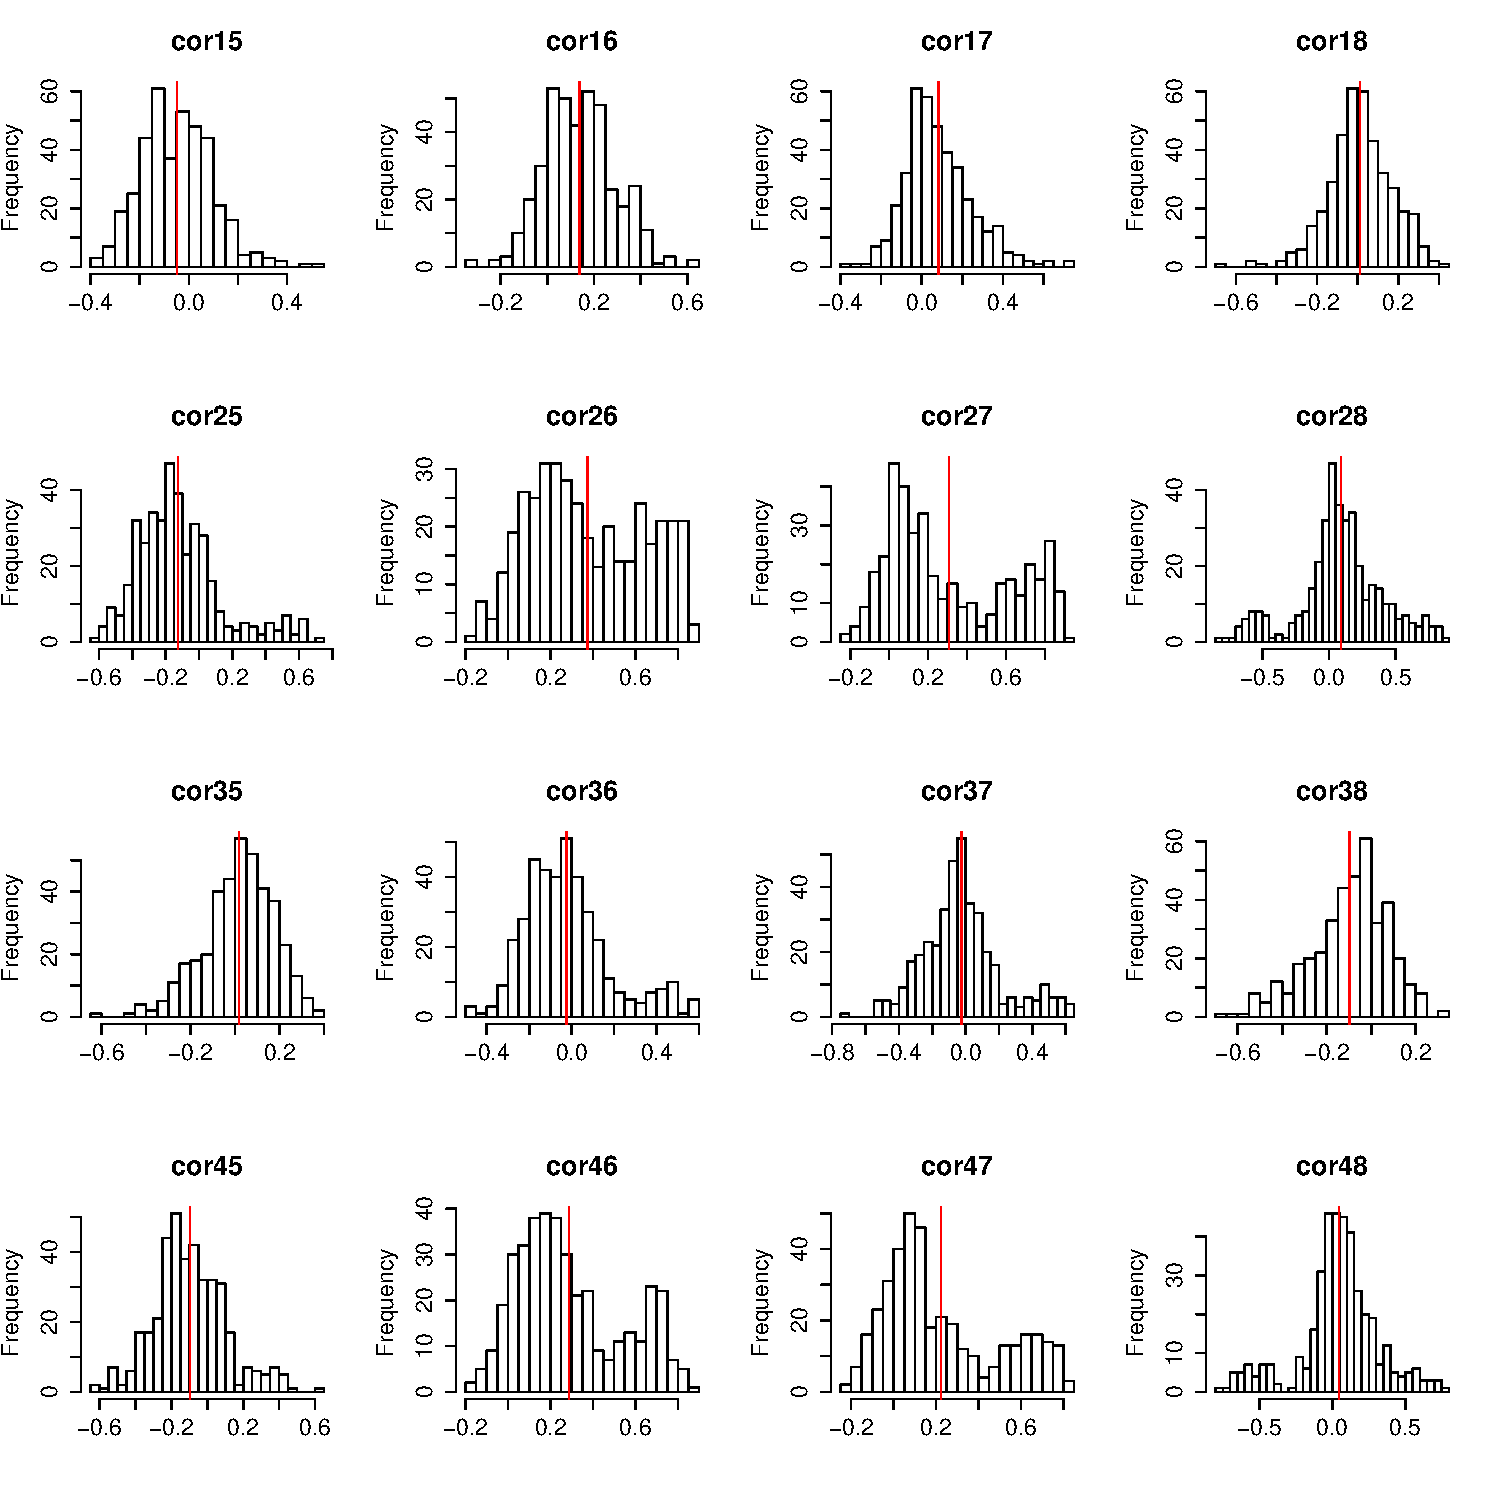
\includegraphics[width=0.35\textwidth]{Figures/PartII/Modeling/CorrelatedData/hist_crossCorMat_breaks30}
%\caption{}
}
\subfloat[]{%[t]{0.23\linewidth}
\vspace{-6.5cm}
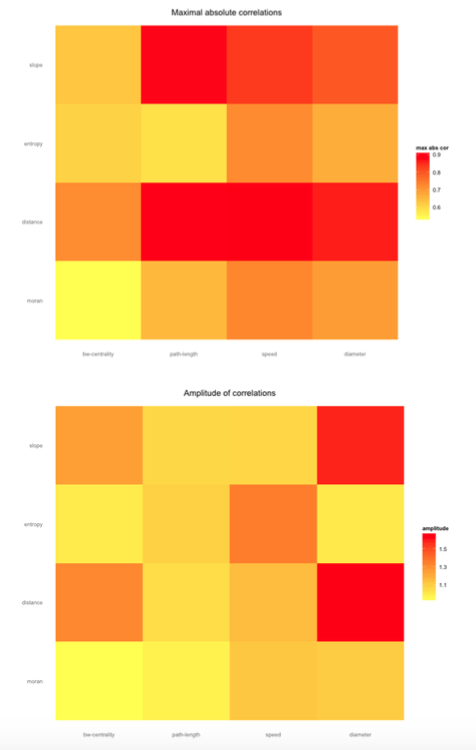
\includegraphics[width=0.23\textwidth]{Figures/PartII/Modeling/CorrelatedData/heatmaps}
}
\subfloat[]{%[t]{0.4\linewidth}
\includegraphics[width=0.4\textwidth]{Figures/PartII/Modeling/CorrelatedData/pca_meanAbsCor_errorBars}
}\\
\subfloat[]{%[t]{0.54\linewidth}
\includegraphics[width=\textwidth]{Figures/PartII/Modeling/CorrelatedData/pca_realDistCol_meanAbsCorSize_withSpecificPoints}
}
\subfloat[]{%[t]{0.45\linewidth}
\vspace{-8.3cm}
}

\caption[Exploration of feasible space for correlations between urban morphology and network structure]{\footnotesize\textbf{Exploration of feasible space for correlations between urban morphology and network structure | } \textbf{(a)} Distribution of crossed-correlations between vectors $\vec{M}$ of morphological indicators (in numbering order Moran index, mean distance, entropy, hierarchy) and $\vec{N}$ of network measures (centrality, mean path length, speed, diameter). \textbf{(b)} Heatmaps for amplitude of correlations, defined as $a_{ij}=\max_k{\rho_{ij}^{(k)}}-\min_k{\rho_{ij}^{(k)}}$ and maximal absolute correlation, defined as $c_{ij}=\max_k\left| \rho_{ij}^{k} \right|$. \textbf{(c)} Projection of correlation matrices in a principal plan obtained by Principal Component Analysis on matrix population (cumulated variances: PC1=38\%, PC2=68\%). Error bars are initially computed as 95\% confidence intervals on each matrix element (by standard Fisher asymptotic method), and upper bounds after transformation are taken in principal plan. Scale color gives mean absolute correlation on full matrices. \textbf{(d)} Representation in the principal plan, scale color giving proximity to real data defined as $1 - \min_r \norm{\vec{M}-\vec{M}_r}$ where $\vec{M}_r$ is the set of real morphological measures, point size giving mean absolute correlation.}{}
\label{fig:densnwcor}
\end{figure}
%%%%%%%%%%%%%%


%%%%%%%%%%%%%%
\begin{figure}
\centering

   \includegraphics[width=0.45\textwidth]{Figures/PartII/Modeling/CorrelatedData/configs/1_param71861_seed0}
   \includegraphics[width=0.45\textwidth]{Figures/PartII/Modeling/CorrelatedData/configs/2_param71913_seed10}\\
   \includegraphics[width=0.45\textwidth]{Figures/PartII/Modeling/CorrelatedData/configs/3_param71918_seed0}
   \includegraphics[width=0.45\textwidth]{Figures/PartII/Modeling/CorrelatedData/configs/4_param71945_seed0}
\caption[Examples of generated coupled configurations]{Configurations obtained for parameters giving the four emphasized points in (d), in order from left to right and top to bottom. We recognize polycentric city configurations (2 and 4), diffuse rural settlements (3) and aggregated weak density area (1). See appendice for exhaustive parameter values, indicators and corresponding correlations. For example $\bar{d}$ is highly correlated with $\bar{l},\bar{s}$ ($\simeq$0.8) in (1) but not for (3) although both correspond to rural environments ; in the urban case we observe also a broad variability : $\rho[\bar{d},\bar{c}]\simeq 0.34$ for (4) but $\simeq-0.41$ for (2), what is explained by a stronger role of gravitation hierarchy in (2) $\gamma=3.9,k_h=0.7$ (for (4), $\gamma=1.07,k_h=0.25$), whereas density parameters are similar.}{}
\end{figure}
%%%%%%%%%%%%%%





%%%%%%%%%%%%%%%%%%%%%%
\subsubsection{Results}{Résultats}


\bpar{
The study of density model alone is developed in~\cite{raimbault2016calibration}. It is in particular calibrated on European density grid data, on 50km width square areas with 500m resolution for which real indicator values have been computed on whole Europe. Furthermore, a grid exploration of model behavior yields feasible output space in reasonable parameters bounds (roughly $\alpha \in [0.5,2],N_G\in [500,3000], P_m \in [10^4,10^5],\beta\in [0,0.2], n_d \in \{ 1, \ldots , 4\}$). The reduction of indicators space to a two dimensional plan through a Principal Component Analysis (variance explained with two components $\simeq 80\%$) allows to isolate a set of output points that covers reasonably precisely real point cloud. It confirms the ability of the model to reproduce morphologically the set of real configurations.
}{
L'étude du modèle de densité seul est développée dans~\cite{raimbault2016calibration}. Il est notamment calibré sur les données de la grille européenne de densité, sur des zones de 50km de côté et de résolution 500m pour lesquelles les valeurs réelles des indicateurs ont été calculées pour l'ensemble de l'Europe. D'autre part, une exploration brutale du modèle permet d'estimer l'ensemble des sorties possibles dans des bornes raisonnables pour les paramètres (grossièrement $\alpha \in [0.5,2],N_G\in [500,3000], P_m \in [10^4,10^5],\beta\in [0,0.2], n_d \in \{ 1, \ldots , 4\}$). La réduction à un plan de l'espace des objectif par une Analyse en Composantes Principales (variance expliquée à deux composantes $\simeq 80\%$) permet d'isoler un nuage de points de sorties recouvrant assez fidèlement le nuage des points réels, ce qui veut dire que le modèle est capable de reproduire morphologiquement l'ensemble des configurations existantes.
}




% NOT NEEDED - TOO MUCH INFORMATION - ?
%%%%%%%%%%%%%%%%
%\begin{figure}
% figure : density example, exploration and calibration ?
%\end{figure}
%%%%%%%%%%%%%%%%


\bpar{
At given density, the conditional exploration of network generation model parameter space suggest a good flexibility on global indicators $\vec{G}$, together with good convergence properties. For a precise study of model behavior, see appendice giving regressions analysis capturing the behavior of coupled model. In order to illustrate synthetic data generation method, the exploration has been oriented towards the study of cross-correlations.
}{
A densité donnée, l'exploration de l'espace des paramètres du modèle de réseau suggèrent une assez bonne flexibilité sur des indicateurs globaux $\vec{G}$, ainsi que de bonnes propriétés de convergence. Pour une étude du comportement précis, voir l'appendice donnant les regressions traduisant le comportement du modèle couplé. Dans le but d'illustrer la méthode de génération de données synthétiques, l'exploration a été orientée vers l'étude des correlations.
}


\bpar{
Given the large relative dimension of parameter space, an exhaustive grid exploration is not possible. We use a Latin Hypercube sampling procedure with bounds given above for $\vec{\alpha}_D$ and for $\vec{\alpha}_N$, we take $N_C \in [50,120], r_g \in [1,100] , d_0 \in [0.1,10] , k_h \in [0,1] , \gamma \in [0.1,4],N_L\in [4,20]$. For number of model replications for each parameter point, less than 50 are enough to obtain confidence intervals at 95\% on indicators of width less than standard deviations. For correlations a hundred give confidence intervals (obtained with Fisher method) of size around 0.4, we take thus $n=80$ for experiments. Figure~\ref{fig:densnwcor} gives details of experiment results. Regarding the subject of correlated synthetic data generation, we can sum up the main lines as following :
\begin{itemize}
\item Empirical distributions of correlation coefficients between morphology and network indicators are not simple and some are bimodal (for example $\rho_{46}=\rho[r,\bar{l}]$  between Moran index and mean path length).
\item it is possible to modulate up to a relatively high level of correlation for all indicators, maximal absolute correlation varying between 0.6 and 0.9. Amplitude of correlations varies between 0.9 and 1.6, allowing a broad spectrum of values. Point cloud in principal plan has a large extent but is not uniform : it is not possible to modulate at will any coefficient as they stay themselves correlated because of underlying generation processes. A more refined study at higher orders (correlation of correlations) would be necessary to precisely understand degrees of freedom in correlation generation.
\item Most correlated points are also the closest to real data, what confirms the intuition and stylized fact of a strong interdependence in reality.
\item Concrete examples taken on particular points in the principal plan show that similar density profiles can yield very different correlation profiles.
\end{itemize}
}{
Etant donné la grande dimension relative de l'espace des paramètres, une exploration par grille exhaustive est impossible. On utilise un plan d'expérience par criblage (hypercube latin), avec les bornes indiquées ci-dessus pour $\vec{\alpha}_D$ et pour $\vec{\alpha}_N$, on a $N_C \in [50,120], r_g \in [1,100] , d_0 \in [0.1,10] , k_h \in [0,1] , \gamma \in [0.1,4],N_L\in [4,20]$. Concernant le nombre de réplications du modèle pour chaque valeur des paramètres, moins de 50 sont nécessaires pour obtenir sur les indicateurs des intervalles de confiance à 95\% de taille inférieure aux déviations standard. Pour les correlations, une centaine donne des IC (obtenus par méthode de Fisher) de taille moyenne 0.4, on fixe donc $n=80$ pour l'expérience. La figure~\ref{fig:densnwcor} donne le détail des résultats de l'exploration. On retiendra les résultats marquants suivants au regard de la génération de données synthétiques corrélées :
\begin{itemize}
\item les distributions empiriques des coefficients de correlations entre indicateurs de forme et indicateurs de réseaux ne sont pas simples, pouvant être bimodales (par exemple $\rho_{46}=\rho[r,\bar{l}]$ entre l'index de Moran et le chemin moyen).
\item On arrive à générer un assez haut niveau de correlation pour l'ensemble des indicateurs, la correlation absolue maximale variant entre 0.6 et 0.9 ; l'amplitude varie quant à elle entre 0.9 et 1.6, ce qui permet un large spectre de valeurs. L'espace couvert dans un plan principal a une étendue certaine mais n'est pas uniforme : on ne peut pas moduler à loisir n'importe quel coefficients, ceux-ci étant liés par les processus de génération sous-jacent. Une étude plus fine aux ordres suivants (correlation des correlations) serait nécessaire pour cerner exactement la latitude dans la génération.
\item les points les plus corrélés en moyenne sont également ceux les plus proches des données réelles, ce qui confirme l'intuition d'une forte interdépendance en réalité.
\item Des exemples concrets pris sur des points particuliers distants dans le plan principal montre que des configurations de densité proches peuvent présenter des profils de correlations très différents.
\end{itemize}
}



%%%%%%%%%%%%%%
%\begin{table}
%regression analysis of param influence on correlations
%  -> Appendice.
%\end{table}
%%%%%%%%%%%%%%




\subsubsection{Possible developments}{Développements}


\bpar{
This case study could be refined by extending correlation control method. A precise knowledge of $N$ behavior (statistical distributions on an exhaustive grid of parameter space) conditional to $D$ would allow to determine $N^{<-1>} | D$ and have more latitude in correlation generation. We could also apply specific exploration algorithms to reach exceptional configurations realizing an expected correlation level, or at least to obtain a better knowledge of the feasible space of correlations~\cite{10.1371/journal.pone.0138212}.
}{
Il est possible de raffiner cette étude en étendant la méthode de contrôle des correlations. La connaissance très fine du comportement de $N$ (distribution statistiques sur une grille fine de l'espace des paramètres) conditionnée à $D$ devrait permettre de déterminer exhaustivement $N^{<-1>} | D$ et avoir plus de latitude dans la génération des correlations. On pourra également appliquer des algorithmes spécifiques d'exploration pour essayer atteindre des configurations exceptionnelles réalisant un niveau de corrélation voulu, ou au moins pour découvrir l'espace des correlations atteignables par la méthode de génération~\cite{10.1371/journal.pone.0138212}.
}



%%%%%%%%%%%%%%%%%%%%%%
\subsection{Discussion}{Discussion}
%%%%%%%%%%%%%%%%%%%%%%



%%%%%%%%%%%%%%%%%%%%%%
\subsubsection{Scientific positioning}{Positionnement Scientifique}

% données hybrides au centre de la démarche d'exploration de modèle, analyse de sensitivité etc.


\bpar{
Our overall approach enters a particular epistemological frame. On the one hand the multidisciplinary aspect, and on the other hand the importance of empirical component through computational exploration methods, make this approach typical of Complex Systems science, as it is recalled by the roadmap for Complex Systems having a similar structure~\cite{2009arXiv0907.2221B}. It combines transversal research questions (horizontal integration of disciplines) with the development of heterogeneous multi-scalar approaches which encounter similar issues as the one we proposed to tackle (vertically integrated disciplines). The combination of empirical knowledge obtained from data mining, with knowledge obtained by modeling and simulation is generally central to the conception and exploration of multi-scalar heterogeneous models. Results presented here is an illustration of such an hybrid paradigm.
}{
Notre démarche s'inscrit dans un cadre épistémologique particulier. En effet, d'une part la volonté de multi-disciplinarité et d'autre part l'importance de la composante empirique couplée aux méthodes d'exploration computationelles, en font une approche typique des sciences de la complexité, comme le rappelle la structure de la feuille de route pour les systèmes complexes~\cite{2009arXiv0907.2221B} qui croise des grandes questions transversales aux disciplines à une intégration verticale de celles-ci, qui implique la construction de modèles multi-échelles hétérogènes présentant souvent les aspects précédent. Le croisement de connaissances empiriques issues de la fouille de données avec celles issues de la simulation est souvent central dans leur conception ou leur exploration, et les résultats présentés ici en sont un exemple typique pour le cas de l'exploration.
}



%%%%%%%%%%%%%%%%%%%%%%
\subsubsection{Direct applications}{Applications Directes}


\bpar{
Starting from the second example which was limited to data generation, we propose examples of direct applications that should give an overview of the range of possibilities.
}{
En partant du deuxième exemple, qui s'est arrêté à la génération des données synthétiques, on peut proposer des pistes d'application directe qui donneront un aperçu de l'éventail des possibilités.
}



\bpar{
\begin{itemize}
\item Calibration of network generation component at given density, on real data for transportation network (typically road network given the shape of generated networks ; it should be straightforward to use OpenStreetMap open data\footnote{\texttt{https://www.openstreetmap.org}} that have a reasonable quality for Europe, at least for France~\cite{girres2010quality}, with however adjustments on generation procedure in order to avoid edge effects due its restrictive frame, for example by generating on an extended surface to keep only a central area on which calibration would be done) should theoretically allow to unveil parameter sets reproducing accurately existing configurations both for urban morphology and network shape. It could be then possible to derive a ``theoretical correlation'' for these, as an empirical correlation is according to some theories of urban systems not computable as a unique realization of stochastic processes is observed. Because of non-ergodicity of urban systems~\cite{pumain2012urban}, there are strong chances that involved processes are different across different geographical areas (or from an other point of view that they are in an other state of meta-parameters, i.e. in an other regime) and that their interpretation as different realizations of the same stochastic process makes no sense, the impossibility of covariation estimation following. By attributing a synthetic dataset similar to a given real configuration, we would be able to compute a sort of \emph{intrinsic correlation} proper to this configuration. As territorial configurations emerge from spatio-temporal interdependences between components of territorial systems, this intrinsic correlation emerges the same way, and its knowledge gives information on these interdependences and thus on relations between territories and networks.
\item As already mentioned, most of models of simulation need an initial state generated artificially as soon as model parametrization is not done completely on real data. An advanced model sensitivity analysis implies a control on parameters for synthetic dataset generation, seen as model meta-parameters~\cite{cottineau2015revisiting}. In the case of a statistical analysis of model outputs it provides a way to operate a second order statistical control.
\item We studied in the first example stochastic processes in the sense of random time-series, whereas time did not have a role in the second case. We can suggest a strong coupling between the two model components (or the construction of an integrated model) and to observe indicators and correlations at different time steps during the generation. In a dynamical spatial models we have because of feedbacks necessarily propagation effects and therefore the existence of lagged interdependences in space and time~\cite{pigozzi1980interurban}. It would drive our field of study towards a better understanding of dynamical correlations.
\end{itemize}
}{
\begin{itemize}
\item La calibration de la composante de génération de réseau, à densité donnée, sur des données réelle de réseau de transport (typiquement routier vu les formes heuristiques obtenues, il devrait par exemple être aisé d'utiliser les données ouvertes d'OpenStreetMap\footnote{\texttt{https://www.openstreetmap.org}} qui sont de qualité raisonnable pour l'Europe, du moins pour la France~\cite{girres2010quality}, avec toutefois des ajustements à faire sur le modèle pour supprimer les effets de bord du à sa structure, par exemple en le faisant générer sur une surface étendue pour ne garder qu'une zone centrale sur laquelle la calibration aurait lieu) permettrait en théorie d'isoler un jeu de paramètres représentant fidèlement des situations existantes à la fois pour la forme urbaine et la forme du réseau. Il serait alors possible de dériver une ``correlation théorique'' pour celles-ci, étant donné qu'une correlation empirique n'est en théorie pas calculable puisqu'une seule instance des processus stochastiques est observée. Vu la non-ergodicité des système urbains~\cite{pumain2012urban}, il y a de fortes chances pour que ces processus soient différents d'une zone géographique à l'autre (ou selon un autre point de vue qu'ils soient dans un autre état des meta-paramètres, dans un autre régime) et que leur interprétation en tant que réalisations d'un même processus stochastique n'ait aucun sens, entrainant l'impossibilité du calcul des covariations. En attribuant un jeu de données synthétiques similaire à une situation donnée, on serait capable de calculer une sorte de \emph{correlation intrinsèque} propre à la situation, qui émerge en fait en réalité des interdépendances temporelles des composantes. Connaitre celle-ci renseigne alors sur ces interdépendances, et donc sur les relations entre réseaux et territoires.
\item Comme déjà évoqué, la plupart des modèles de simulation nécessitent un état initial, généré artificiellement à partir du moment où la paramétrisation n'est pas effectuée totalement à partir de données réelles. Une analyse de sensibilité avancée du modèle implique alors un contrôle sur les paramètres de génération du jeu de données synthétique, vu comme méta-paramètre du modèle~\cite{cottineau2015revisiting}. Dans le cas d'une analyse statistique des sorties du modèle, on est alors capable d'effectuer un contrôle statistique au second ordre.
\item On a étudié des processus stochastiques dans le premier exemple, au sens de séries temporelles aléatoires, alors que le temps ne jouait pas de rôle dans le second. On peut suggérer un couplage fort entre les deux composantes du modèle (ou la construction d'un modèle intégré) et observer les indicateurs et correlations à différents pas de temps de la génération. Dans le cas d'une dynamique, de par les rétroactions, on a nécessairement des effets de propagation et donc l'existence d'interdépendances décalées dans l'espace et le temps~\cite{pigozzi1980interurban}, étendant le domaine d'étude vers une meilleure compréhensions des correlations dynamiques.
\end{itemize}
}




%%%%%%%%%%%%%%%%%%%%%%
\subsubsection{Generalization}{Généralisation}


\bpar{
We were limited to the control of first and second moments of generated data, but we could imagine a theoretical generalization allowing the control of moments at any order. However, as shown by the geographical example, the difficulty of generation in a concrete complex case questions the possibility of higher orders control when keeping a consistent structure model and a reasonable number of parameters. The study of non-linear dependence structures as proposed in~\cite{chicheportiche2013nested} is in an other perspective an interesting possible development.
}{
On s'est limité au contrôle des premiers et second moments des données générées, mais il est possible d'imaginer une généralisation théorique permettant le contrôle des moments à un ordre arbitraire. Toutefois, la difficulté de génération dans un cas concret complexe, comme le montre l'exemple géographique, questionne la possibilité de contrôle aux ordres supérieurs tout en gardant un modèle à la structure cohérente au au nombre de paramètres relativement faibles. Par contre, l'étude de structures de dépendances non-linéaires comme celles utilisées dans~\cite{chicheportiche2013nested} est une piste de développement intéressante.
}


%%%%%%%%%%%%%%%%%%%%%%
%\subsection*{Autres domaines potentiels d'application}
% ideas of other fields where the generation can happen.
% -> not necessary, suggested in intro ?



%%%%%%%%%%%%%%%%%%%%%%
\subsection{Conclusion}{Conclusion}
%%%%%%%%%%%%%%%%%%%%%%


\bpar{
We described a model allowing to generate synthetic datasets in which correlation structure is controlled. Its exploration shows its flexibility and the broad range of possible applications. More generally, it is crucial to favorise such practices of systematic validation of computational models by statistical analysis, in particular for agent-based models for which the question of validation stays an open issue. 
}{
On a ainsi proposé une méthode abstraite de génération de données synthétiques corrélées à un niveau contrôlé. Son implémentation partielle dans deux domaines très différents montre sa flexibilité et l'éventail des applications potentielles. De manière générale, il est essentiel de généraliser de telles pratiques de validation systématique de modèles par étude statistique, en particulier pour les modèles agents pour lesquels la question de la validation reste encore relativement ouverte.
}



%--------------------------------------

% Section : benchmarking of network growth models

\newpage

\section[Network Growth Models]{Network Growth Models : Explicative power for various approaches}{Modèles de Croissance de Réseau}

\subsection{Benchmarking Network growth heuristics}{Comparer les heuristiques de croissance de réseau}


\bpar{
Considering Network Growth in itself, many heuristics are available to generate a network under some constraints. As already developed, from economic network growth approach to local optimization heuristics, geographical mechanisms or biological network growth, each has its advantages and particularities. We plan to compare these varied methods against real network indicators values for the european road network. We present in Fig.~\ref{fig:slimemould} a preliminary work done in~\cite{raimbault2015labex} to explore implementation of the biological network growth models. Also the implementation of local optimization models was explored, typically the one described in the methodology section on reproducibility. 
}{
Pour la croissance du réseau en tant que tel, de nombreuses heuristiques existent pour générer un réseaux sous certaines contraintes. Comme déjà développé précédemment, des modèles économiques de croissance de réseau au heuristiques d'optimisation locale, aux mécanismes géographiques ou à la croissance de réseau biologique, chacun a ses avantages et particularités propres. Un travail futur aura pour but de comparer ces diverses méthodes contres les valeurs réelles des indicateurs pour le réseau de routes européen. La Fig.~\ref{fig:slimemould} présente un travail préliminaire présenté dans~\cite{raimbault2015labex} qui explore des applications des modèles de croissance de réseau biologique. D'autre part, comme présenté dans la section sur la reproductibilité, des modèles d'optimisation locale ont également été testés.
}


%%%%%%%%%%%%%%%%%%%%%%
\begin{figure}
\includegraphics[width=0.45\textwidth]{Figures/PartII/Modeling/NetworkGrowth/tick1}
\includegraphics[width=0.45\textwidth]{Figures/PartII/Modeling/NetworkGrowth/tick20}\\
\includegraphics[width=0.45\textwidth]{Figures/PartII/Modeling/NetworkGrowth/tick50}
\includegraphics[width=0.45\textwidth]{Figures/PartII/Modeling/NetworkGrowth/reseauFinal}
\caption[Biological Network Growth]{Example of the application of the slime mould network generation model to the computation of an optimal public transportation network design.}{}
\label{fig:slimemould}
\end{figure}
%%%%%%%%%%%%%%%%%%%%%%%






\subsection{Towards simple models of network morphogenesis}{Vers des modèles simples de morphogenèse de réseau}

An interdisciplinary project that was just launched with a Physicist \noun{Lagesse}, an Architect \noun{Hachi} and a Computer Scientist \noun{Dugue} aims at finding consistent models of urban street network morphogenesis, regarding urban design particularities, geographical rules and complex network indicators feedbacks. Models of network morphogenesis were already discuss here and the aim of this project is to gain insight from the interdisciplinary vision to explore the potentiality of such models. In the frame of our thesis, it is logically situated within the morphogenesis theoretical part and network growth modeling heuristics.















%%%%%%%%%%%%%%%
% Lutecia : particular case including specific thematic developments





% Chapter 

\chapter{Towards more Complex Models} % Chapter title

\label{ch:complexmodels} % For referencing the chapter elsewhere, use \autoref{ch:name} 


%----------------------------------------------------------------------------------------

This single section chapter is differentiated from the previous one as it makes a step further towards more complex models. A toy-model introducing governance processes is described. Such exploration logically enters our theoretical framework to try to validate or invalidate the network necessity assumption : if non-linear necessary processes are highlighted and validated against stylized facts, it argues towards the validation of this assumption. 

Other targeted projects such as the exploration of an hybrid macro-economic/accessibility-based model to explore transportation companies line implementation strategies are still at the state of ideas and are not described here.



%----------------------------------------------------------------------------------------


\section[The Lutecia Model]{Taking Governance into account in Network Production Processes : The Lutecia Model}{Le Modèle Lutecia}


%%%%%%%%%%%%%%%%%%
\subsection{Thematic Context}


We describe a game-theory based framework, studied in collaboration with \noun{Le Nechet} which aims to be integrated as behavioral rules for governing agents in a hybrid model introduced in~\cite{le2010approche} and formalized then explored in~\cite{lenechet2012}. This model couples land-use dynamics with transportation infrastructure evolution and aims to endogeneize transportation infrastructure development at different levels. The framework proposed extends it by allowing cooperation and fusion between governing entities.



As detailed in~\cite{lenechet2012}, a conceptual city system with local administrative boundaries and corresponding governing agents (mayors), and a global governor (state) is the foundation of the model. A land-use evolution (residences and employments localisations) and transportation (gravity flows) are the first step of an iteration. The transportation infrastructure (road network) is then evolved by constructing a new road. First level of decision (global or local) is chosen randomly according to a fixed probability, and in the case of a local decision, the richest mayor will build the new road. The road is then build optimizing the marginal accessibility for the area corresponding to the builder in charge (all world if global, commun if local).

One thematic aspect lacking in the model and that would be interesting to study is the emergence of larger administrative zones, i.e. the emergence of new levels of governance in polycentric metropolitan areas. The reality is of course not as simple, as bottom-up initiatives such as collaboration between neighbor cities are interlaced with top-down decisions such as e.g. the ``M{\'e}tropole du Grand Paris'' which is a new administrative structure for Paris Area decided at the state level~\cite{gilli2009paris}. It would be however interesting to test conditions for emergence of governance patterns from the bottom-up in a conceptual way by extending the model and adding interactions and fusion between administrative entities.

The extension shall consist in relaxing the assumption of a single road segment built at each time step and attribute one segment to the $N$ richest mayors. That leads to situation where neighbor towns may want to construct both a new road. As they are likely to communicate with each other, we assume that negotiations take place and that they consider eventually to build in common, in which case they merge after (rough simplifying but stylized assumption). Such negotiations may be interpreted as a game in the sense of Game Theory, which as already been widely applied for modeling in social and political sciences for questions dealing with cognitive interacting agents with individual interests~\cite{ordeshook1986game}. Such a framework as already been used in transportation investment studies, as e.g. in~\cite{Roumboutsos2008209} where choices of operators (public and privates) to integrate their system in a global consistent commuter system is explored through the notion of Nash equilibrium.

% \cite{2016arXiv161208111S} : rationale for staying at two players : games with many become chaotic




\subsection{Formalization}


The model architecture couples in a complex way a module for land-use evolution with a module for transportation network growth. Submodules, detailed in the following, include in particular a governance module that rules processes of network evolution.


\subsubsection{Land-use evolution}

The following steps are detailed in~\cite{lenechet2012} but we recall the big picture :

\begin{itemize}
\item Initial distribution of Actives and Employments is done around governance centers at positions $\vec{x}_i$ by
\[
A(\vec{x}) = A_{max} \cdot \exp{\left(\frac{\norm{\vec{x}-\vec{x}_i}}{r_A}\right)} ; 
E(\vec{x}) = E_{max} \cdot \exp{\left(\frac{\norm{\vec{x}-\vec{x}_i}}{r_E}\right)}
\]

\item For facility patches, employments are added by $E(\vec{x}) = E(\vec{x})+\frac{k_{ext}\cdot E_{max}}{n_{ext}}$.

\item Transportation module : computation of flows $\phi_{ij}$ are done by solving on $p_i,q_j$ by a fixed point method (Furness algorithm), the system of gravity flows
\[
\begin{cases}
\phi_{ij} = p_i q_j A_i E_j \exp{\left(-\lambda_{tr} d_{ij}\right)}\\
\sum_k \phi_{kj} = E_j ; \sum_k \phi_{ik} = A_i\\
p_i = \frac{1}{\sum_k{q_k E_k \exp{(-\lambda_{tr}d_{ik})}}} ; q_j = \frac{1}{\sum_k{p_k A_k \exp{(-\lambda_{tr}d_{kj})}}} 
\end{cases}
\]

\item Trajectories then attributed by effective shortest path, and corresponding congestion $c$ obtained (no Wardrop equilibrium). 

\item Speed of network is given by a BPR function $v(c) = v_0 \left(1 - \frac{c}{\kappa}\right)^{\gamma_c}$. Congestion is not used in current studies (infinite capacity $\kappa$).

\item Land-Use module : we assume that residential/employments relocations are at equilibrium at the time scale of a tick, that corresponds to transportation infrastructure evolution time scale which is much larger~\cite{bretagnolle:tel-00459720}.

\item We take a Cobb-douglas function for utilities of actives/employments at a given cell
\[
U_i (A) = X_i(A)^{\gamma_A}\cdot {F_i(A)}^{1-\gamma_A} ; F_i(A) = \frac{1}{A_i E_i}
\]
\[
U_j (E) = X_j(E)^{\gamma_E}\cdot {F_j(E)}^{1-\gamma_E} ; F_j(E) = 1
\]

where $X_i(A) = A_i\cdot \sum_j{E_j \exp{\left(-\lambda\cdot d_{ij}\right)}}$ and $X_j(E) = E_j\cdot \sum_i{A_i \exp{\left(-\lambda\cdot d_{ij}\right)}}$.

\item Relocations are then done deterministically following a discrete choice model :
\[
A_i(t+1) = \sum_i{A_i(t)}\cdot\frac{\exp{(\beta U_i(A))}}{\sum_i{\exp{(\beta U_i(A))}}}
\]
\[
E_j(t+1) = \sum_j{E_j(t)}\cdot\frac{\exp{(\beta U_j(E))}}{\sum_j{\exp{(\beta U_j(E))}}}
\]

\end{itemize}


The default parameter values are taken as follows : $A_{max} = E_{max} = 500 ; r_A = 1 ; r_E = 0.8 ; \gamma_E = 0.9 ; \gamma_A = 0.65 ; \beta_{l} = 1.8 ; \lambda = 0.005 ; r_0 = 2$

and 
 
$N_{expl} = 25 ; I = 0.001 ; J = 0.0001 ; \nu = 5 ; E_{ext}(t_0) = 3E_{max} ; t_f = 4$


%%%%%%%%%%%%%%%%%%%%%
%% Dynamic programming
%%%%%%%%%%%%%%%%%%%%%

\subsubsection{Effective distances computation}

Distance via network are updated in a dynamical programming fashion for efficiency purposes (because of the numerous network updates), the following way :

\begin{itemize}
\item Euclidian distance matrix $d(i,j)$ computed analytically
\item Network shortest paths between network intersections (rasterized network) updated in a dynamic way (addition of new paths and update/change of old paths if needed when a link is added), correspondance between network patches and closest intersection also updated dynamically ; $O(N_{inters}^3)$
\item Weak component clusters and distance between clusters updated ; $O(N_{nw}^2)$
\item Network distances between network patches updated, through the heuristic of only minimal connexions between clusters ; $O(N_{nw}^2)$
\item Effective distances (taking paces/congestion into account) updated as minimum between euclidian time and \[\min_{C,C'}{d(i,C)+d_{nw}(p_C(i),p_C'(j))+d(C',j)}\], complexity in $O(N_{clusters}^2\cdot N^2)$ (Approximated with $\min_C$ only in the implementation, consistent within the interaction ranges $\sim$ 5 patches taken in the model). 
\end{itemize}



\subsubsection{Externality}

The model allows also to simulate the competition of territory for an external ressource (an airport for example). We implement therefore the option of adding in initial state an area with initial $A_{max}$ employments and that follows an intrinsic growth rule as a geometric law. 



\subsubsection{Transportation Network growth}


The workflow for transportation network development is the following :

\begin{itemize}

\item At each time step, $N$ new road segments are built. Choice between local and global is still done through uniform drawing with probability $\xi$. In the case of local building, roads are attributed successively to mayors with probabilities $\xi_i$, what means that richer areas may get many roads. It stays consistent with the thematic assumption than each road correspond to the allocation of one public market which are done independently (with $N$ becoming greater, this assumption should be relaxed as attribution of subventions to local areas is of course not proportional to wealth, but we assume that it stays true with small $N$ values). 

\item Areas building a road without neighbors doing it follow the standard procedure to develop the road network.

\item Neighbor areas building a road will enter negotiations. We assume in this first simple version of the model that only bilateral negotiations may occur. Therefore, in the case of clusters with more than two areas, pairing is done at random (uniform drawing) between neighbors until all areas are paired.

\item Possible strategies for players (negotiating areas, $i=1,2$) are : staying alone ($A$) and collaborating ($C$). Strategies are chosen simultaneously (non-cooperative game) as detailed after. For $(C,A)$ and $(A,C)$ couples, the collaborating agent loose its investment and cannot build a road whereas the other continues his business alone. For $(A,A)$ both act as alone, and for $(C,C)$ a common development is done. We denote $Z^{\ast}_i(S_1,S_2)$ the optimal infrastructure for area $i$ with $(S_1,S_2)\in \{(A,C),(C,A),(A,A)\}$ which are determined the standard way in each zone separately, and $Z^{\ast}_C$ the optimal common infrastructure computed with a 2 segments infrastructure on the union of both areas, which corresponds to the case where both strategies are $C$. Marginal accessibilities for area $i$ and infrastructure $Z$ is defined as $\Delta X_i(Z)=X^Z_i - X_i$. We introduce the costs of construction which are necessary to build the payoff matrix. They are assumed spatially uniform and noted $I$ for a road segment, whereas a 2 road segment will cost $2\cdot I - \delta I$ ($\delta I > 0$ cost gain of common technical means, assumed to be equally shared). An interesting generalization would be to divise costs proportional to wealth in the case of a collaboration. The payoff matrix of the game is the following, with $\kappa$ a normalization constant (``price of accessibility'') :

\medskip
\hfill
\begin{tabular}{ |c|c|c| } 

 \hline
 1 $|$ 2  & C & A \\ \hline
 C & $U_i = \kappa \cdot \Delta X_i(Z^{\ast}_C) - I - \frac{\delta I}{2}$
   & $\begin{cases}U_1 = \kappa \cdot \Delta X_1(Z^{\ast}_1)-I \\U_2 = \kappa \cdot \Delta X_2(Z^{\ast}_2)-I - \frac{\delta I}{2}\end{cases}$ \\ \hline
 A & $\begin{cases}U_1 = \kappa \cdot \Delta X_1(Z^{\ast}_1)-I - \frac{\delta I}{2}\\U_2 = \kappa \cdot \Delta X_2(Z^{\ast}_2)-I\end{cases}$
   & $U_i = \kappa \cdot \Delta X_i(Z^{\ast}_i) - I$ \\
 \hline
\end{tabular}
\hfill\hfill
\medskip

We have a typical coordination game for which it is clear that no strategy is dominant for any player. In a probabilistic mixed-strategy case, there always exists a Nash equilibrium that we can easily determine in our case. It is reasonable to make such an assumption since negotiations take generally some time during which agents are able to find the way to optimize rationally their expected utility. If $\Pb{S_1=C} = p_1$ and $\Pb{S_2=C} = p_2$, we have

\[
\begin{split}
\Eb{U_1} & =p_1 p_2 U_1(C,C) + p_1\cdot (1-p_2) U_1(C,A) + p_2 \cdot (1-p_1) U_1(A,C) + (1-p_1)(1-p_2) U_1(A,A)\\
& = p_1 \cdot \left[ p_2 \cdot \left(\kappa \cdot \Delta X_1(Z^{\ast}_C) - \frac{\delta I}{2} \right) - \kappa \cdot \Delta X_1(Z^{\ast}_1) + I\right] + p_2\cdot\frac{\delta I}{2} + \kappa\cdot\Delta X_1(Z^{\ast}_1)-I
\end{split}
\]

Optimizing the expected utility along $p_1$ (the variable on which agent 1 has control) imposes the condition on $p_2$

\[
\frac{\partial \Eb{U_1}}{\partial p_1} = 0 \iff p_2 = \frac{\delta I / 2}{\Delta X_{\bar{2}}{Z^{\star}_{C}} - \Delta X_{\bar{2}}{Z^{\star}_{\bar{2}}}}
\]

We obtain generally

\[
p_i = \frac{J}{\Delta X_{\bar{i}}{Z^{\star}_{C}} - \Delta X_{\bar{i}}{Z^{\star}_{\bar{i}}}}
\]

Note that we can directly interpret these expressions, as a player chances to cooperate will decrease with the potential gain of the other player, what is intuitive for a competitive game. It also forces feasibility conditions on $I$ and $\delta I$ to keep a probability, that are $I \leq \kappa\cdot \min(\Delta X_1(Z^{\ast}_1),\Delta X_2(Z^{\ast}_2))$ (binary positive cost-benefit conditions) and $I-\delta I > \kappa \cdot \max_i (\Delta X_i(Z^{\ast}_i)-\Delta X_i(Z^{\ast}_C))$. As soon as accessibility difference stay relatively small, both shall be compatible when $\delta I \ll I$, giving corresponding boundaries for $I$.

\item Agents make choice of strategy following uniform drawings with probability computed above. Corresponding infrastructures are built, and in the case of choices $(C,C)$, towns merge in a single one with new corresponding variables (employment, actives, etc. ).


\end{itemize}



\paragraph{Remark for the implementation}

To adapt an existing implementation, one just has to add the negotiation stage if conditions are met, using probabilities given above. The accessibility-dimensioned parameters $\alpha = \frac{I}{\kappa}$ and $\delta \alpha = \frac{\delta I}{\kappa}$ should be more simple to deal with.



% TODO : insert a mechanisms with NO DC framework as reference/benchmark/null model ?

\paragraph{An alternative discrete choice ``game''}

Using the same payoff matrix with a random utility model allows to obtain also values for probabilities. We have

\[
U_i(C) - U_i(NC) = p_{\bar{i}} \left( \Delta X_{i}{Z^{\star}_{C}} - \Delta X_{i}{Z^{\star}_{i}}\right) - J
\]

and therefore $p_i$ verifies the equation that is solved numerically

\[
p_i = \frac{1}{1 + \exp{\left(-\beta_{DC}\cdot \left(\frac{\Delta X_{i}{Z^{\star}_{C}} - \Delta X_{i}{Z^{\star}_{i}}}{1 + \exp{\left(- \beta_{DC}(p_i \cdot (\Delta X_{\bar{i}}{Z^{\star}_{C}} - \Delta X_{\bar{i}}{Z^{\star}_{\bar{i}}}) - J)\right)}} - J \right)\right)}}
\]

This module is also implemented for comparison purposes.


\subsection{Results}

% validation at different levels ; exploration etc.  - to be relaunched -

\subsubsection{Implementation}

The model was implemented in \texttt{NetLogo}~\cite{wilensky1999netlogo} because of its exploratory and interactive nature. A particular care was taken for the computation of accessibilities and shortest paths, as a dynamic reevaluation of network distance is necessary for each new potential infrastructure, what become rapidly a computational burden. We use thus a dynamical programming shortest path computation, inspired from~\cite{tretyakov2011fast}, using distance matrices updates instead of shortest paths full computation at each step. See details in architectural precisions in Appendix~\ref{app:bibliography}


%%%%%%%%%%
\begin{figure}
\includegraphics[width=0.5\textwidth]{Figures/PartII/Modeling/Lutecia/ex_collab_0}
\includegraphics[width=0.5\textwidth]{Figures/PartII/Modeling/Lutecia/ex_dc_finalCollab}\\
\includegraphics[width=0.5\textwidth]{Figures/PartII/Modeling/Lutecia/ex_simpleNash_0}
\includegraphics[width=0.5\textwidth]{Figures/PartII/Modeling/Lutecia/example_nocollab_0}
\caption[Examples of final configurations]{Examples of final configurations, with or without externality, for different values of cooperation parameters.}
\label{fig:luteciaexample}
\end{figure}
%%%%%%%%%%


%%%%%%%%%%
\begin{figure}
\includegraphics[width=0.5\textwidth]{Figures/PartII/Modeling/Lutecia/_MEAN_ACC}
\includegraphics[width=0.5\textwidth]{Figures/PartII/Modeling/Lutecia/_NW_FREQ}
\caption[Validation of network exploration heuristic]{Validation of network exploration heuristic : mean accessibility(left) and network positions on 500 realizations on the same initial configuration. The optimal distribution of network validates network generation heuristic.}
\label{fig:luteciavalid}
\end{figure}
%%%%%%%%%%%



\subsubsection{Exploration and Validation}

We show in Fig.~\ref{fig:luteciaexample} and Fig.\ref{fig:luteciavalid} examples of obtained configurations and preliminary validation of governance and network growth heuristic. Internal validation and external validation through stylized facts, and model explorations, including statistical analysis of model behavior, are provisory for now and not presented here (see~\cite{le2015modeling} for preliminary results).


%\subsection{Perspectives}
% why is this model useful for the following













%% Chapter 3

\chapter{Math Test Chapter} % Chapter title

\label{ch:mathtest} % For referencing the chapter elsewhere, use \autoref{ch:mathtest}

%----------------------------------------------------------------------------------------

\lipsum[13]

%----------------------------------------------------------------------------------------

\section{Some Formulas}

Due to the statistical nature of ionisation energy loss, large fluctuations can occur in the amount of energy deposited by a particle traversing an absorber element\footnote{Examples taken from Walter Schmidt's great gallery: \\ \url{http://home.vrweb.de/~was/mathfonts.html}}.  Continuous processes such as multiple scattering and energy loss play a relevant role in the longitudinal and lateral development of electromagnetic and hadronic showers, and in the case of sampling calorimeters the measured resolution can be significantly affected by such fluctuations in their active layers.  The description of ionisation fluctuations is characterised by the significance parameter $\kappa$, which is proportional to the ratio of mean energy loss to the maximum allowed energy transfer in a single collision with an atomic electron: \graffito{You might get unexpected results using math in chapter or section heads. Consider the \texttt{pdfspacing} option.}
\begin{equation}
\kappa =\frac{\xi}{E_{\mathrm{max}}} %\mathbb{ZNR}
\end{equation}
$E_{\mathrm{max}}$ is the maximum transferable energy in a single collision with an atomic electron.
\[E_{\mathrm{max}} =\frac{2 m_{\mathrm{e}} \beta^2\gamma^2 }{1 + 2\gamma m_{\mathrm{e}}/m_{\mathrm{x}} + \left ( m_{\mathrm{e}} /m_{\mathrm{x}}\right)^2}\ ,\]
where $\gamma = E/m_{\mathrm{x}}$, $E$ is energy and $m_{\mathrm{x}}$ the mass of the incident particle, $\beta^2 = 1 - 1/\gamma^2$ and $m_{\mathrm{e}}$ is the electron mass. $\xi$ comes from the Rutherford scattering cross section and is defined as:
\begin{eqnarray*} \xi  = \frac{2\pi z^2 e^4 N_{\mathrm{Av}} Z \rho
\delta x}{m_{\mathrm{e}} \beta^2 c^2 A} =  153.4 \frac{z^2}{\beta^2}
\frac{Z}{A}
\rho \delta x \quad\mathrm{keV},
\end{eqnarray*}
where

\begin{tabular}{ll}
$z$ & charge of the incident particle \\
$N_{\mathrm{Av}}$ & Avogadro's number \\
$Z$ & atomic number of the material \\
$A$ & atomic weight of the material \\
$\rho$ & density \\
$ \delta x$ & thickness of the material \\
\end{tabular}

$\kappa$ measures the contribution of the collisions with energy transfer close to $E_{\mathrm{max}}$.  For a given absorber, $\kappa$ tends towards large values if $\delta x$ is large and/or if $\beta$ is small.  Likewise, $\kappa$ tends towards zero if $\delta x $ is small and/or if $\beta$ approaches $1$.

The value of $\kappa$ distinguishes two regimes which occur in the description of ionisation fluctuations:

\begin{enumerate}
\item A large number of collisions involving the loss of all or most of the incident particle energy during the traversal of an absorber.

As the total energy transfer is composed of a multitude of small energy losses, we can apply the central limit theorem and describe the fluctuations by a Gaussian distribution. This case is applicable to non-relativistic particles and is described by the inequality $\kappa > 10 $ (\ie, when the mean energy loss in the absorber is greater than the maximum energy transfer in a single collision).

\item Particles traversing thin counters and incident electrons under any conditions.

The relevant inequalities and distributions are $ 0.01 < \kappa < 10 $, Vavilov distribution, and $\kappa < 0.01 $, Landau distribution.
\end{enumerate}

%----------------------------------------------------------------------------------------

\section{Various Mathematical Examples}

If $n > 2$, the identity \[t[u_1,\dots,u_n] = t\bigl[t[u_1,\dots,u_{n_1}], t[u_2,\dots,u_n] \bigr]\] defines $t[u_1,\dots,u_n]$ recursively, and it can be shown that the alternative definition \[t[u_1,\dots,u_n] = t\bigl[t[u_1,u_2],\dots,t[u_{n-1},u_n]\bigr]\] gives the same result. % Chapter 4 - empty template

\cleardoublepage % Empty page before the start of the next part


%------------------------------------------------

\ctparttext{This concluding remark, for now a brief roadmap, is one objective of our thesis as implementation of our theory ans thus is expected to become a consequent part. We conclude here this preliminary work by perspectives and roadmap.} % Text on the Part 2 page describing the content in Part 2


% Part III : Towards operational models
%\part{Towards operational models}
\part{Synthesis : towards a delicate though robust edifice}


%  A family of dynamic models : develop aim.

%  Various case studies : develop launched/potential collaborations




% introduction de la partie 

\section*{A Roadmap for an Operational Family of Models of Coevolution}{Vers des Modèles Opérationnels de Coevolution} % Chapter title

\label{ch:operational}

%----------------------------------------------------------------------------------------

As previously stated, one of our principal aims is the validation of the network necessity assumption, that is the differentiating point with a classic evolutive urban theory. To do so, toy-model exploration and empirical analysis will not be enough as hybrid models are generally necessary to draw effective and well validated conclusions. We briefly give an overview of planned work in the following, that will be the conclusion of this Memoire.



%----------------------------------------------------------------------------------------



\section*{Objectives}{Objectifs}


We expect to product \emph{models of coevolution}, \comment{(Florent) expliciter la différence avec ce que tu as fait jusque là}
 with the emphasis on processes of coevolution, to directly confront the theory. They will be necessary a flexible family because of the variety of scales and concrete cases we can include and we already began to explore in preliminary studies. Processes already studied can serve either as a thematic bases for a reuse as building bricks in a multi-modeling context, or as methodological tools such as synthetic data generator for synthetic control. Finally, we mean by operational models hybrid models, in the sense of semi-parametrized or semi-calibrated on real datasets or on precise stylized facts extracted from these same datasets. This point is a requirement to obtain a thematic feedback on geographical processes and on theory.


%----------------------------------------------------------------------------------------

\section*{Case Studies}{Cas d'étude}

Currently we expect to work on the following case studies to build these hybrid models :

\begin{itemize}
\item Dynamical data for Bassin Parisien should allow to parametrize and calibrate a model at this temporal and spatial scale.
\item On larger scales, South African dataset of \noun{Baffi} will along empirical analysis also be used to parametrize hybrid co-evolution models.
\item A possibility that is not currently set up (and that may however be difficult because of a disturbing closed-data policy among a frightening large number of scientists !) is the exploitation of French railway growth dataset (with population dataset) used in~\cite{bretagnolle:tel-00459720}, that would also provide an interesting case study on other regimes, scales and transportation mode.
\end{itemize}



%----------------------------------------------------------------------------------------



\section*{Roadmap}{Feuille de Route}


We give the following (non-exhaustive and provisory) roadmap for modeling explorations (theoretical and empirical domains being still explored conjointly) :

\begin{enumerate}
\item Complete the exploration of independent and weak coupled urban growth and network growth processes (all models presented in chapter~\ref{ch:modeling}), in order to know precisely involved mechanisms when they are virtually isolated, and to obtain morphogenesis scales.
\item Go further into the exploration of toy-model of non conventional processes such as governance network growth heuristic to pave the road for a possible integration of such modules in hybrid models.
\item Build a Marius-like generic infrastructure that implement the theory in a family of models that can be declined into diverse case studies.
\item Launch it and adapt it on these case studies.
\end{enumerate}

Next steps would be too hypothetical if formulated, we propose thus to proceed iteratively in our construction of knowledge and naturally update this roadmap constantly.

\bigskip
\bigskip
\bigskip

\textit{ - La route est longue mais la voie est libre.}










\cleardoublepage

%------------------------------------------------

\ctparttext{A building is never used the way it was designed, that is a reality which grasping makes the difference between good and excellent architects. So does a knowledge edifice. We shall now take a look back on what we constructed and try to take a step back. This part develops first theoretical apparels emerging from the various aspects already tackled. It then proposes to extract fundamental open questions that future research on territorial complex systems will have to tackle in the incoming decades.}


% Opening
\part{Opening : effective functional use give sense to any construction}
% this part should make a "meta-synthesis" (include here theories ? and research project for the future - lines of research and fundamental questions)


\cleardoublepage

%------------------------------------------------

%\ctparttext{}


% Conclusion
%\part*{Conclusion}





%------------------------------------------------
% Provisory chapters 





%------------------------------------------------
% Bibliography


\cleardoublepage
% Bibliography

\label{app:bibliography} % Reference the bibliography elsewhere with \autoref{app:bibliography}

\manualmark % Work-around to have small caps also here in the headline
\markboth{\spacedlowsmallcaps{\bibname}}{\spacedlowsmallcaps{\bibname}} % Work-around to have small caps also
\phantomsection
\refstepcounter{dummy}

\addtocontents{toc}{\protect\vspace{\beforebibskip}} % Place the bibliography slightly below the rest of the document content in the table of contents
\addcontentsline{toc}{chapter}{\tocEntry{\bibname}}



\printbibliography % Bibliography



%----------------------------------------------------------------------------------------
%	THESIS CONTENT - APPENDICES
%----------------------------------------------------------------------------------------

%\appendix

\part{Appendix} % New part of the thesis for the appendix


%%%%%%%%%%%%%%%%%%
%% Appendix : Synthetic Data (introduction and financial development)

\section{Generation of Correlated Synthetic Data}{Generation of Correlated Synthetic Data} % Chapter title

\label{app:syntheticdata} % For referencing the chapter elsewhere, use \autoref{ch:name} 

%----------------------------------------------------------------------------------------




%%%%%%%%%%%%%%%%%%%%%%
\subsection*{Application : financial time-series}{Application : Séries temporelles financières}


%%%%%%%%%%%%%%%%%%%%%%
\subsubsection*{Context}{Contexte}

\bpar{
Our first field of application is that of financial complex systems, of which captured signals, financial time-series, are heterogeneous, multi-scalar and highly non-stationary~\cite{mantegna2000introduction}. Correlations have already been the object of a broad bunch of related literature. For example, Random Matrix Theory allows to undress signal of noise, or at least to estimate the proportion of information undistinguishable from noise, for a correlation matrix computed for a large number of asset with low-frequency signals (daily returns mostly)~\cite{2009arXiv0910.1205B}. Similarly, Complex Network Analysis on networks constructed from correlations, by methods such as Minimal Spanning Tree~\cite{2001PhyA..299...16B} or more refined extensions developed for this purpose~\cite{tumminello2005tool}, yielded promising results such as the reconstruction of economic sectors structure. At high frequency, the precise estimation of of interdependence parameters in the framed of fixed assumptions on asset dynamics, has been extensively studied from a theoretical point of view aimed at refinement of models and estimators~\cite{barndorff2011multivariate}. Theoretical results must be tested on synthetic datasets as they ensure a control of most parameters in order to check that a predicted effect is indeed observable \emph{all things equal otherwise}. For example, \cite{potiron2015estimation} obtains a bias correction for the \emph{Hayashi-Yoshida} estimator (used to estimate integrated covariation between two brownian at high frequency in the case of asynchronous observation times) by deriving a central limit theorem for a general model that endogeneize observation times. Empirical confirmation of estimator improvement is obtained on a synthetic dataset at a fixed correlation level.
}{
Un premier domaine d'application proposé pour notre méthode est celui des séries temporelles financières, signaux typiques de systèmes complexes hétérogènes et multiscalaires~\cite{mantegna2000introduction} et pour lesquels les corrélations ont fait l'objet d'abondants travaux. Ainsi, l'application de la théorie des matrices aléatoires peut permettre de débruiter, ou du moins d'estimer la part de signal noyée dans le bruit, une matrice de correlations pour un grand nombre d'actifs échantillonnés à faible fréquence (retours journaliers par exemple)~\cite{2009arXiv0910.1205B}. De même, l'analyse de réseaux complexes construits à partir des corrélations, selon des méthodes type arbre couvrant minimal~\cite{2001PhyA..299...16B} ou des extensions raffinées pour cette application précise~\cite{tumminello2005tool}, ont permis d'obtenir des résultats prometteurs, tels la reconstruction de la structure économique des secteurs d'activités. A haute fréquence, l'estimation précise de paramètres d'interdépendance dans le cadre d'hypothèses fixées sur la dynamique, fait l'objet d'importants travaux théoriques dans un but de raffinement des modèles et des estimateurs~\cite{barndorff2011multivariate}. Les résultats théoriques doivent alors être testés sur des jeux de données synthétiques, qui permettent de contrôler un certain nombre de paramètres et de s'assurer qu'un effet prédit par la théorie est bien observable \emph{toutes choses égales par ailleurs}. Par exemple, \cite{potiron2015estimation} dérive une correction du biais de l'estimateur de \emph{Hayashi-Yoshida} qui est un estimateur de la covariance de deux browniens corrélés à haute fréquence dans le cas de temps d'observation asynchrones, par démonstration d'un théorème de la limite centrale pour un modèle généralisé endogénéisant les temps d'observations. La confirmation empirique de l'amélioration de l'estimateur est alors obtenue sur un jeu de données synthétiques à un niveau de corrélation fixé.
}


%%%%%%%%%%%%%%%%%%%%%%
\subsubsection*{Formalization}{Formalisation}

\paragraph{Framework}{Cadre}


\bpar{
We consider a network of assets $(X_i(t))_{1\leq i \leq N}$ sampled at high-frequency (typically 1s). We use a multi-scalar framework (used e.g. in wavelet analysis approaches~\cite{ramsey2002wavelets} or in multi-fractal signal processing~\cite{bouchaud2000apparent}) to interpret observed signals as the superposition of components at different time scales : $X_i=\sum_{\omega}{X_i^{\omega}}$. We denote by $T_i^{\omega} = \sum_{\omega' \leq \omega} X_i^{\omega}$ the filtered signal at a given frequency $\omega$. A recurrent problem in the study of complex systems is the prediction of a trend at a given scale. It can be viewed as the identification of regularities and their distinction from components considered as random\footnote{see~\cite{gell1995quark} for an extended discussion on the construction of \emph{schema} to study complex adaptive systems (by complex adaptive systems).}. For the sake of simplicity, we represent such a process as a trend prediction model at a given temporal scale $\omega_1$, formally an estimator $M_{\omega_1} : (T_i^{\omega_1}(t'))_{t'<t} \mapsto \hat{T_i}^{\omega_1}(t)$ which aims to minimize error on the real trend $\norm{T_i^{\omega_1} - \hat{T}_i^{\omega_1}}$. In the case of autoregressive multivariate estimators, the performance will depend among other parameters on respective correlations between assets. It is thus interesting to apply the method to the evaluation of performance as a function of correlation at different scales. We assume a Black-Scholes dynamic for assets~\cite{jarrow1999honor}, i.e. $dX = \sigma\cdot dW$, with $W$ Wiener process. Such a dynamic model allows an easy modulation of correlation levels.
}{
Considérons un réseau d'actifs $(X_i(t))_{1\leq i \leq N}$ échantillonnés à haute fréquence (typiquement 1s). On se place dans un cadre multi-scalaire (utilisé par exemple dans les approches par ondelettes~\cite{ramsey2002wavelets} ou analyses multifractales du signal~\cite{bouchaud2000apparent}) pour interpréter les signaux observés comme la superposition de composantes à des multiples échelles temporelles : $X_i=\sum_{\omega}{X_i^{\omega}}$. On notera $T_i^{\omega} = \sum_{\omega' \leq \omega} X_i^{\omega}$ le signal filtré à une fréquence $\omega$ donnée. Prédire l'évolution d'une composante à une échelle donnée est alors un problème caractéristique de l'étude des systèmes complexes, pour lequel l'enjeu est l'identification de régularités et leur distinction des composantes considérées comme stochastiques en comparaison\footnote{voir~\cite{gell1995quark} pour une discussion étendue sur la construction de \emph{schema} pour l'étude de systèmes complexes adaptatifs (par des systèmes complexes adaptatifs).}. Dans un souci de simplicité, on représente un tel processus par un modèle de prédiction de tendance à une échelle temporelle $\omega_1$ donnée, formellement un estimateur $M_{\omega_1} : (T_i^{\omega_1}(t'))_{t'<t} \mapsto \hat{T_i}^{\omega_1}(t)$ dont l'objectif est la minimisation de l'erreur sur la tendance réelle $\norm{T_i^{\omega_1} - \hat{T}_i^{\omega_1}}$. Dans le cas d'estimateurs auto-regressifs multivariés, la performance dépendra entre autre des correlations respectives entre actifs et il est alors intéressant d'utiliser la méthode pour évaluer celle-ci en fonction de niveaux de correlation à plusieurs échelles. On assume une dynamique de Black-Scholes~\cite{jarrow1999honor} pour les actifs, i.e. $dX = \sigma\cdot dW$ avec $W$ processus de Wiener, ce qui permettra d'obtenir facilement des niveaux de correlation voulus.
}


\paragraph{Data generation}{Génération des données}


\bpar{
We can straightforward generate $\tilde{X}_i$ such that $\Varb{\tilde{X}_i^{\omega_1}}=\Sigma R \Sigma$ (with $\Sigma$ estimated standard deviations and $R$ fixed correlation matrix) and verifying $X_i^{\omega \leq \omega_0} = \tilde{X}_i^{\omega \leq \omega_0}$ (data proximity indicator : components at a lower frequency than a fundamental frequency $\omega_0 < \omega_1$ are identical). We use therefore the simulation of Wiener processes with fixed correlation. Indeed, if $dW_1 \indep dW_1^{\indep}$ (and $\sigma_1 < \sigma_2$ indicatively, assets being interchangeable), then
\[
W_2 = \rho_{12}W_1 + \sqrt{1-\frac{\sigma_1^2}{\sigma_2^2}\cdot\rho_{12}^2}\cdot W_1^{\indep}
\]
is such that $\rho(dW_1,dW_2)=\rho_{12}$. Next signals are constructed the same way by Gram orthonormalization. We isolate the component at the desired frequency $\omega_1$ by filtering the signal, i.e. $\tilde{X}_i^{\omega_1} = W_i - \mathcal{F}_{\omega_0}[W_i]$ (with $\mathcal{F}_{\omega_0}$ low-pass filter with cut-off frequency $\omega_0$). We reconstruct then the hybrid synthetic signals by 
\begin{equation}
\tilde{X}_i = T_i^{\omega_0} + \tilde{X}_i^{\omega_1}
\end{equation}
}{
Il est alors aisé de générer $\tilde{X}_i$ tel que $\Varb{\tilde{X}_i^{\omega_1}}=\Sigma R$ ($\Sigma$ variance estimée et $R$ matrice de corrélation fixée), par la simulation de processus de Wiener au niveau de corrélation fixé et tel que $X_i^{\omega \leq \omega_0} = \tilde{X}_i^{\omega \leq \omega_0}$ (critère de proximité au données : les composantes à plus basse fréquence qu'une fréquence fondamentale $\omega_0 < \omega_1$ sont identiques). En effet, si $dW_1 \indep dW_1^{\indep}$ (et $\sigma_1 < \sigma_2$ pour fixer les idées, quitte à échanger les actifs), alors $W_2 = \rho_{12}W_1 + \sqrt{1-\frac{\sigma_1^2}{\sigma_2^2}\cdot\rho_{12}^2}W_1^{\indep}$ est tel que $\rho(dW_1,dW_2)=\rho_{12}$. Les signaux suivants sont construits de la même manière par orthonormalisation de Gram. On isole alors la composante à la fréquence $\omega_1$ voulue par filtrage, c'est à dire $\tilde{X}_i^{\omega_1} = W_i - \mathcal{F}_{\omega_0}[W_i]$ (avec $\mathcal{F}_{\omega_0}$ filtre passe-bas à fréquence de coupage $\omega_0$), puis on reconstruit les signaux synthétiques par $\tilde{X}_i = T_i^{\omega_0} + \tilde{X}_i^{\omega_1}$.
}




\subsubsection{Implementation and Results}{Implémentation et résultats}

\paragraph{Methodology}{Méthodologie}



\bpar{
The method is tested on an example with two assets from foreign exchange market (EUR/USD and EUR/GBP), in a six month period from June 2015 to November 2015. Data\footnote{obtained from \texttt{http://www.histdata.com/}, without specified licence. For the respect of copyright, only cleaned and filtered at $\omega_m$ data are made openly available.} cleaning, starting from original series sampled at a frequency around 1s, consists in a first step to the determination of the minimal common temporal range (missing sequences being ignored, by vertical translation of series, i.e. $S(t):=S(t)\cdot \frac{S(t_{n})}{S(t_{n-1})}$ when $t_{n-1},t_n$ are extremities of the ``hole'' and $S(t)$ value of the asset, what is equivalent to keep the constraint to have returns at similar temporal steps between assets). We study then \emph{log-prices} and \emph{log-returns}, defined by $X(t):=\log{\frac{S(t)}{S_0}}$ and $\Delta X (t) = X(t) - X(t-1)$. Raw data are filtered at a maximal frequency $\omega_m = 10\textrm{min}$ (which will be the maximal frequency for following treatments) for concerns of computational efficiency\footnote{as time-series are then sampled at $3\cdot\omega_m$ to avoid aliasing, a day of size 86400 for 1s sampling is reduced to a much smaller size of 432.}. We use a non-causal gaussian filter of total width $\omega$. We fix the fundamental frequency $\omega_0=24\textrm{h}$ and we propose to construct synthetic data at frequencies $\omega_1 = 30\textrm{min},1\textrm{h},2\textrm{h}$. See Fig.~\ref{fig:example_signal} for an example of signal structure at these different scales.
}{
La méthode est testée sur un exemple de deux actifs du marché des devises (EUR/USD et EUR/GBP), sur une période de 6 mois de juin 2015 à novembre 2015. Le nettoyage des données\footnote{obtenues depuis \texttt{http://www.histdata.com/}, sans licence spécifiée, les données nettoyées et filtrées à $\omega_m$ uniquement sont mises en accessibilité pour respect du copyright.}, originellement échantillonnées à l'ordre de la seconde, consiste dans un premier temps à la détermination du support temporel commun maximal (les séquences manquantes étant alors ignorées, par translation verticale des séries, i.e. $S(t):=S(t)\cdot \frac{S(t_{n})}{S(t_{n-1})}$ lorsque $t_{n-1},t_n$ sont les extrémités du ``trou'' et $S(t)$ la valeur de l'actif, ce qui revient à garder la contrainte d'avoir des retours à pas de temps similaires entre actifs).On étudie alors les \emph{log-prix} et \emph{log-retours}, définis par $X(t):=\log{\frac{S(t)}{S_0}}$ et $\Delta X (t) = X(t) - X(t-1)$. Les données brutes sont filtrées à une fréquence $\omega_m = 10\textrm{min}$ (qui sera la fréquence maximale d'étude) pour un souci de performance computationnelle. On utilise un filtre gaussien non causal de largeur totale $\omega$. On fixe $\omega_0=24\textrm{h}$ et on se propose de construire des données synthétiques aux fréquences $\omega_1 = 30\textrm{min},1\textrm{h},2\textrm{h}$. Voir la figure~\ref{fig:example_signal} pour un exemple de la structure du signal à ce différentes échelles.
}


%%%%%%%%%%%%%%%%%%%
\begin{figure}%[h!]
\centering
\includegraphics[width=\textwidth]{Figures/SyntheticData/ex_filtering}
\caption[Example of the multi-scalar structure of the signal]{\textbf{Example of the multi-scalar structure of the signal, basis of the construction of synthetic signals | } \emph{Log-prices} are represented on a time window of around 3h for November 1st 2015 for asset EUR/USD, with 10min (purple) and 30min trends.}{}
\label{fig:example_signal}
\end{figure}
%%%%%%%%%%%%%%%%%%%

% TODO : Q add examples of synthetic signal ?


\bpar{
It is crucial to consider the interference between $\omega_0$ and $\omega_1$ frequencies in the reconstructed signal : correlation indeed estimated is 
\[
\rho_{e} = \rho \left[ \Delta \tilde{X}_1 , \Delta \tilde{X}_2 \right] = \rho \left[ \Delta T_1^{\omega_0} + \Delta \tilde{X}_1^{\omega} , \Delta T_2^{\omega_0} + \Delta \tilde{X}_2^{\omega}\right]
\]
what yields in the reasonable limit $\sigma_1 \gg \sigma_0$ (fundamental frequency small enough), when $\Covb{\Delta \tilde{X}_i^{\omega_1}}{\Delta X_j^{\omega}}=0$ for all $i,j,\omega_1 > \omega$ and returns centered at any scale, the correction on effective correlation due to interferences : we have at first order the expression of effective correlation

\begin{equation}
\label{eq:eff_corr}
\rho_e = \left[ \varepsilon_1 \varepsilon_2 \rho_0 + \rho \right] \cdot \left[ 1 - \frac{1}{2}\left(\varepsilon_1^2 + \varepsilon_2^2 \right) \right]
\end{equation}

{\noindent}what gives the correlation that we can effectively simulate in synthetic data.
}{
Il est crucial de noter l'interférence entre les fréquences $\omega_0$ et $\omega_1$ dans le signal construit : la correlation effectivement estimée est
\[
\rho_{e} = \rho \left[ \Delta \tilde{X}_1 , \Delta \tilde{X}_2 \right] = \rho \left[ \Delta T_1^{\omega_0} + \Delta \tilde{X}_1^{\omega} , \Delta T_2^{\omega_0} + \Delta \tilde{X}_2^{\omega}\right]
\]
ce qui conduit à dériver dans la limite raisonnable $\sigma_1 \gg \sigma_0$ (fréquence fondamentale suffisamment basse), lorsque $\Covb{\Delta \tilde{X}_i^{\omega_1}}{\Delta X_j^{\omega}}=0$ pour tous $i,j,\omega_1 > \omega$, et les retours d'espérance nulle à toutes échelles, en notant $\rho_0 = \rho \left[ \Delta T_1^{\omega_0} , \Delta T_2^{\omega_0} \right]$, $\rho = \rho \left[  \tilde{X}_1^{\omega_1} , \tilde{X}_2^{\omega_1} \right]$, et $\varepsilon_i = \frac{\sigma (\Delta T_i^{\omega_0})}{\sigma \left( \Delta \tilde{X}_i^{\omega_1}\right)}$, la correction sur la correlation effective due aux interférences : la correlation effective est alors au premier ordre

\begin{equation}
\label{eq:eff_corr}
\rho_e = \left[ \varepsilon_1 \varepsilon_2 \rho_0 + \rho \right] \cdot \left[ 1 - \frac{1}{2}\left(\varepsilon_1^2 + \varepsilon_2^2 \right) \right]
\end{equation}

{\noindent}ce qui donne l'expression de la correlation que l'on pourra effectivement simuler dans les données synthétiques.
}


\bpar{
Correlation is estimated by Pearson method, with estimator for covariance corrected for bias, i.e.
\[
\hat{\rho}[X1,X2] = \frac{\hat{C}[X1,X2]}{\sqrt{\hat{\Var{}}[X1]\hat{\Var{}}[X2]}}\]
, where $\hat{C}[X1,X2] = \frac{1}{(T-1)}\sum_{t} X_1(t)X_2(t) - \frac{1}{T\cdot (T-1)} \sum_t X_1(t) \sum_t X_2(t)$ and $\hat{\Var{}}[X] = \frac{1}{T}\sum_t{X^2(t)}-\left(\frac{1}{T}\sum_tX(t)\right)^2$.
}{
La correlation est estimée par méthode de Pearson, avec l'estimateur de la covariance au biais corrigé, c'est à dire $\hat{\rho}[X1,X2] = \frac{\hat{C}[X1,X2]}{\sqrt{\hat{\Var{}}[X1]\hat{\Var{}}[X2]}}$, où $\hat{C}[X1,X2] = \frac{1}{(T-1)}\sum_{t} X_1(t)X_2(t) - \frac{1}{T\cdot (T-1)} \sum_t X_1(t) \sum_t X_2(t)$ et $\hat{\Var{}}[X] = \frac{1}{T}\sum_t{X^2(t)}-\left(\frac{1}{T}\sum_tX(t)\right)^2$.
}



\bpar{
The tested predictive model $M_{\omega_1}$ is a simple \emph{ARMA} for which parameters $p=2,q=0$ are fixed (as we do not create lagged correlation, we do not expect large orders of auto-regression as these kind of processes have short memory for real data ; furthermore smoothing is not necessary as data are already filtered). It is however applied in an adaptive way\footnote{adaptation level staying low, as parameters $T_W,p,q$ and model type do not vary. We are positioned within the framework of~\cite{potiron2016estimating} which assumes a locally parametric dynamic but for which meta-parameters are fixed. We could imagine a variable $T_W$ which would adapt for the best local fit, the same way parameters are estimated in bayesian signal processing by augmentation of the state with parameters.}. More precisely, given a time window $T_W$, we estimate for any $t$ the model on $[t-T_W+1,t]$ in order to predict signals at $t+1$.
}{
Le modèle de prédiction $M_{\omega_1}$ testé est simplement un modèle \emph{ARMA} pour lequel on fixe les paramètres $p=2,q=0$ (on ne créée pas de correlation retardée, on ne s'attend donc pas à de grand ordre d'auto-regression, les signaux originaux étant à mémoire relativement courte ; de plus le lissage n'est pas nécessaire puisqu'on travaille sur des données filtrées), appliqué de manière adaptative\footnote{il s'agit d'un niveau d'adaptation relativement faible, les paramètres $T_W,p,q$ et même le type de modèle restant fixés. On se place ainsi dans le cadre de~\cite{potiron2016estimating} qui suppose une dynamique localement paramétrique, mais pour lequel on fixe les méta-paramètres de la dynamique. On pourrait imaginer estimer un $T_W$ variable qui s'adapterait pour une meilleure estimation locale, à l'image de l'estimation de paramètres en traitement du signal Bayesien effectuée via augmentation de l'état par les paramètres.}. Plus précisément, étant donné une fenêtre temporelle $T_W$, on estime pour tout $t$ le modèle sur $[t-T_W+1,t]$ afin de prédire les signaux à $t+1$.
}


\paragraph{Implementation}{Implémentation}


\bpar{
Experiments are implemented in \texttt{R} language, using in particular the \texttt{MTS}~\cite{Tsay:2015xy} library for time-series models. Cleaned data and source code are openly available on the \texttt{git} repository of the project\footnote{at \texttt{https://github.com/JusteRaimbault/SynthAsset}}. 
}{
L'implémentation est faite en language R, utilisant en particulier la bibliothèque \texttt{MTS}~\cite{Tsay:2015xy} pour les modèles de séries temporelles. Les données nettoyées et le code source sont disponibles de manière ouverte sur le dépôt \texttt{git} du projet\footnote{at \texttt{https://github.com/JusteRaimbault/SynthAsset}}.
}



\paragraph{Results}{Résultats}



\bpar{
Figure~\ref{fig:effective_corrs} gives effective correlations computed on synthetic data. For standard parameter values (for example $\omega_0=24\textrm{h}$, $\omega_1=2\textrm{h}$ and $\rho=-0.5$), we find $\rho_0\simeq 0.71$ et $\varepsilon_i \simeq 0.3$ what yields $\left| \rho_e - \rho \right|\simeq 0.05$. We observe a good agreement between observed $\rho_e$ and values predicted by~\ref{eq:eff_corr} in the interval $\rho \in [-0.5,0.5]$. On the contrary, for larger absolute values, a deviation increasing with $\left|\rho\right|$ and as $\omega_1$ decreases : it confirms the intuition that when frequency decreases and becomes closer to $\omega_0$, interferences between the two components are not negligible anymore and invalidate independence assumptions for example. 
}{
La figure~\ref{fig:synthdata:effective_corrs} donne les correlations effectives calculées sur les données synthétiques. Pour des valeurs standard des paramètres (par exemple pour $\omega_0=24\textrm{h}$, $\omega_1=2\textrm{h}$ et $\rho=-0.5$), on a $\rho_0\simeq 0.71$ et $\varepsilon_i \simeq 0.3$ et ainsi $\left| \rho_e - \rho \right|\simeq 0.05$. On constate dans l'intervalle $\rho \in [-0.5,0.5]$ un bon accord entre la valeur $\rho_e$ prédite par~\ref{eq:eff_corr} et les valeurs observées, et une déviation pour de plus grandes valeurs absolues, d'autant plus grande que $\omega_1$ est petit : cela confirme l'intuition que lorsque la fréquence descend et se rapproche de $\omega_0$, les interférences entre les deux composantes vont devenir non négligeables et invalider les hypothèses d'indépendance par exemple.
}


\bpar{
We apply then the predictive model described above to synthetic data, in order to study its mean performance as a function of correlation between signals. Results for $\omega_1 = 1\textrm{h},1\textrm{h}30,2\textrm{h}$ are shown in Fig.~\ref{fig:model_perf}. The a priori counter-intuitive result of a maximal performance at vanishing correlation for one of the assets confirms the role of synthetic data to better understand system mechanisms : the study of lagged correlations shows an asymmetry in the real data that we can understand at a daily scale as an increased influence of EUR/GBP on EUR/USD with a rough two hours lag. The existence of this \emph{lag} allows a ``good'' prediction of EUR/USD thanks to fundamental component. This predictive power is perturbed by added noises in a way that increases with their correlation. The more noises correlated are, the more he model will take them into account and will make false predictions because of the markovian character of simulated brownian\footnote{the model used has theoretically no predictive power at all on pure brownian}.
}{
On applique ensuite le modèle prédictif décrit ci-dessus aux données synthétiques, afin d'étudier sa performance moyenne en fonction du niveau de correlation des données. Les résultats pour $\omega_1 = 1\textrm{h},1\textrm{h}30,2\textrm{h}$ sont présentés en figure~\ref{fig:model_perf}. Le résultat a priori contre-intuitif d'une performance maximale à correlation nulle pour l'un des actifs confirme l'intérêt d'une génération de données hybrides : l'étude des correlations décalées (\emph{lagged correlations}) montre une dissymétrie présente dans les données réelles, interprété à l'échelle journalière comme une influence augmentée de EURGBP sur EURUSD à 2h de décalage environ. L'existence de ce \emph{lag} permet une ``bonne'' prédiction de EURUSD due à la fréquence fondamentale, perturbée par le bruit ajouté, de façon proportionnelle à sa correlation : plus les bruits sont corrélés, plus le modèle les prendra en compte et se trompera plus à cause du caractère markovien des browniens simulés\footnote{en théorie le modèle utilisé n'a aucun pouvoir prédictif sur des browniens purs}.
}


\bpar{
This case study stays a \emph{toy-model} and has no direct practical application, but demonstrates however the relevance of using simulated synthetic data. Further developments can be directed towards the simulation of more realistic data (presence of consistent \emph{lagged correlation} patterns, more realistic models than Black-Scholes) and apply it on more operational predictive models.
}{
L'exemple présenté ici est un \emph{modèle jouet} et n'a pas d'application pratique, mais démontre l'intérêt de l'utilisation des données synthétiques simulées. On peut imaginer simuler des données plus proches de la réalité (existence de motifs réalistes de \emph{lagged correlation} par exemple, modèles plus réalistes que le Black-Scholes) et appliquer la méthode sur des modèles plus opérationnels.
}




%%%%%%%%%%%%%%%%%%%
\begin{figure}[h!]
\centering
% figure : effective correlations, with confidence intervals (bootstrap), for the 3 filtering scales. ; AND expected corrected corrs from derivation above.
%\vspace{-0.7cm}
\includegraphics[width=\textwidth]{Figures/SyntheticData/effectiveCorrs_withGoodTh_A4}
\caption[Effective correlations obtained on synthetic data]{\small\textbf{Effective correlations obtained on synthetic data | } Dots represent estimated correlations on a synthetic dataset corresponding to 6 months between June and November 2015 (error-bars give 95\% confidence intervals obtained with standard Fisher method) ; scale color gives filtering frequency $\omega_1=10\textrm{min},30\textrm{min},1\textrm{h},2\textrm{h},4\textrm{h}$ ; solid lines give theoretical values for $\rho_e$ obtained by~\ref{eq:eff_corr} with estimated volatilities (dotted-line diagonal for reference) ; vertical red line position is the theoretical value such that $\rho = \rho_e$ with mean values for $\varepsilon_i$ on all points. We observe for high absolute correlations values a deviation from corrected values, what should be caused by non-verified independence and centered returns assumptions. Asymmetry is caused by the high value of $\rho_0 \simeq 0.71$.}{}
\label{fig:effective_corrs}
\end{figure}
%%%%%%%%%%%%%%%%%%%


%%%%%%%%%%%%%%%%%%%
\begin{figure}[h!]
% figure : performance of arma2 as a function of expected correlation.
%\vspace{-0.7cm}
\centering
\includegraphics[width=0.48\textwidth,height=0.16\textheight]{Figures/SyntheticData/pred_filt6}
\includegraphics[width=0.48\textwidth,height=0.16\textheight]{Figures/SyntheticData/pred_filt9}\\
\includegraphics[width=0.48\textwidth,height=0.16\textheight]{Figures/SyntheticData/pred_filt12}
\includegraphics[width=0.48\textwidth,height=0.16\textheight]{Figures/SyntheticData/lagged_corrs}
\caption[Performance of a predictive model as a function of simulated correlations]{\small \textbf{Performance of a predictive model as a function of simulated correlations | } From left to right and top to bottom, three first graphs show for each asset the normalized performance of an ARMA model ($p=2,q=0$), defined as $\pi = \left(\frac{1}{T}\sum_t\left(\tilde{X}_i(t) - M_{\omega_1}\left[\tilde{X}_i\right](t)\right)^2 \right) / \sigma \left[ \tilde{X}_i \right]^2$ (95\% confidence intervals computed by $\pi = \bar{\pi} \pm (1.96\cdot \sigma [\pi])/\sqrt{T}$, local polynomial smoothing to ease reading). It is interesting to note the U-shape for EUR/USD, due to interference between components at different scales. Correlation between simulated noises deteriorates predictive power. The study of \emph{lagged correlations} (here $\rho [\Delta X_{\textrm{EURUSD}}(t),\Delta X_{\textrm{EURGBP}}(t-\tau)]$) on real data clarifies this phenomenon : fourth graph show an asymmetry in curves at any scale compared to zero lag $(\tau = 0)$ what leads fundamental components to increase predictive power for the dollar, amelioration then perturbed by correlations between simulated components. Dashed lines show time steps (in equivalent $\tau$ units) used by the ARMA at each scale, what allows to read the corresponding lagged correlation on fundamental component.}{}
\label{fig:model_perf}
\end{figure}
%%%%%%%%%%%%%%%%%%%







 % provisory
%%%%%%%%%%%%%%%%%%

%%%%%%%%%%%%%%%%%%
%% Appendix : Morphogenesis
%


% Chapter 

%\chapter{Urban Morphogenesis}{Morphogenèse Urbaine} % Chapter title
\chapter{Morphogenèse Urbaine}

\label{ch:morphogenesis} % For referencing the chapter elsewhere, use \autoref{ch:name} 

%----------------------------------------------------------------------------------------

%\headercit{}{}{}

%\bigskip


Il est bien établi en géographie l'importance des relations spatiales et de la mise en réseau, comme le formule \noun{Tobler} par sa ``première loi de la géographie''~\cite{tobler2004first}. Nous l'avons mis en évidence pour les relations entre réseaux et territoires par exemple en section~\ref{sec:interactiongibrat}. Toutefois, les travaux sur la non-stationnarité et la non-ergodicité, ainsi que la mise en valeur d'échelles locales endogènes, suggèrent une certaine pertinence à l'idée de sous-système relativement indépendant, au sens où il serait possible d'isoler certaines règles locales régissant celui-ci étant fixés certains paramètres exogène capturant justement les relations avec d'autres sous-systèmes. Cette question porte à la fois sur l'échelle d'espace, de temps, mais aussi sur les éléments concernés. Reprenons un exemple concret de terrain déjà évoqué en Chapitre~\ref{ch:thematic}: la laborieuse mise en place du tramway de Zhuhai. L'impact du retard de la mise en place et la remise en question de futures lignes, dus à un problème technique inattendu lié à une technologie de transfert de courant par troisième rail importée d'Europe qui n'avait jamais été testée dans les conditions climatiques locales, assez exceptionnelles en termes d'humidité, aura une nature très différentes selon l'échelle et les agents considérés. Le manque de coordination générale entre transports et urbanisme laisse supposer que les dynamiques urbaines en terme de populations et d'emplois y sont relativement insensibles à court terme. Le Bureau des Transports de la Municipalité ainsi que le bureau technique Européen ont pu subir des répercussions politiques et économiques bien plus graves. D'autre part, que ce soit à Zhongshan, Macao ou Hong-Kong le problème a une repercussion quasi-nulle. Généralisant au système de transport local, celui-ci peut être relativement bien isolé des systèmes voisins ou à plus grande échelle, et donc ses relations avec la ville considérées dans un contexte locale. On supposera à la fois une certaine forme de stationnarité locale (``régime urbain local'') mais aussi une certaine indépendance avec l'extérieur. Dans ce cadre, son auto-organisation locale impliquera nécessairement des relations fortes entre forme et fonction, de par la distribution spatiale des fonctions urbaines mais aussi car \emph{la forme fait la fonction} dans certains cas de figure, au sens des motifs d'utilisation entièrement conditionnés à cette forme. Le type de raisonnement que nous avons esquissé mobilise les éléments essentiels propres à l'idée de \emph{morphogenèse urbaine}. Nous allons dans ce chapitre clarifier sa définition et montrer les potentialité qu'elle donne pour éclairer les relations entre réseaux et territoires. La morphogenèse, qui a été importée de la biologie vers de nombreux champs, a dans chaque cas ouvert des voies pour l'étude des systèmes complexes propres à ce champ selon un point particulier. Il est important de noter que le monument qu'est la Théorie des Catastrophes de \noun{René Thom} introduit une façon originale de comprendre la différentiation qualitative et donc la morphogenèse. Cette théorie, très mal comprise, contient un potentiel d'application immense aux problèmes qui nous concernent, comme l'a effleuré \noun{Durand-Dastès}~\cite{durand2003geographes} en évoquant la systèmogenèse, que nous développerons en ouverture. Dans un premier temps, un effort d'épistémologie par des points de vue complémentaires de plusieurs disciplines permet d'éclairer la nature de la morphogenèse dans la section~\ref{sec:interdiscmorphogenesis}. Cela permet de clarifier le concept en lui donnant une définition bien précise, distincte de celle de l'auto-organisation, qui appuie les relations causales circulaires entre forme et fonction. Nous explorons ensuite un modèle simple de morphogenèse urbaine, basé sur la densité de population seule, à l'échelle mesoscopique, dans la section~\ref{sec:densitygeneration}. La démonstration que les processus abstraits d'agrégation et de diffusion sont suffisants pour reproduire l'ensemble des formes d'établissements humains en Europe, en utilisant les résultats de~\ref{sec:staticcorrelations}, confirme la pertinence de l'idée de morphogenèse pour la modélisation à certaines échelles et pour certains aspects. Ce modèle est ensuite couplé de manière séquentielle à un module de morphogenèse de réseau dans la section~\ref{sec:correlatedsyntheticdata}, afin d'établir un espace faisable des correlations statiques entre indicateurs de forme urbaine et indicateurs de réseau, qui sont comme on l'a vu précédemment un témoin des relations locales entre réseaux et territoires. Celui-ci s'avère relativement large, ce qui confirmera l'utilisation de ce type de modèle de manière fortement couplée par la suite.




\stars


\textit{Ce chapitre est composé de divers travaux. La première section est adaptée d'un travail en anglais en collaboration avec \noun{C. Antelope}, \noun{L. Hubatsch} et \noun{J.M. Serna} à la suite de l'école d'été 2016 du Santa Fe Institute~\cite{antelope2016interdisciplinary}; la deuxième section est traduite de~\cite{}; et enfin la troisième section a été écrite pour les Actes des Journées de Rochebrune 2016~\cite{raimbault2016generation}.}





%----------------------------------------------------------------------------------------









 % provisory
%%%%%%%%%%%%%%%%%%



%%%%%%%%%%%%%%%%%%
%% Appendix : technical developments
\chapter{Technical Developments} % Chapter title

\label{app:technical} % For referencing the chapter elsewhere, use \autoref{ch:name} 

%----------------------------------------------------------------------------------------


\headercit{C'est hardcore tes calculs.}{Anonyme}{}



This chapter gathers various technical developments, that have the common points to be not essential to the core of the thesis and difficult to digest.


\section{Derivations for Urban Growth Models}





\begin{lemma}
The limit of a Preferential Attachment model when $\lambda \ll 1$ is a linear-growth Gibrat model, with limit parameters $\mu_i(t)=1+\frac{\lambda}{m\cdot (t-1)}$.
\end{lemma}

\begin{proof}

Starting with first moment, we denote $\bar{P}_i(t)=\Eb{P_i(t)}$. Independence of Gibrat growth rate yields directly $\bar{P}_i(t)=\Eb{R_i(t)}\cdot \bar{P}_i(t-1)$. Starting for the preferential attachment model, we have $\bar{P}_i(t) = \Eb{P_i(t)} = \sum_{k=0}^{+\infty}{k\Pb{P_i(t)=k}}$. But
\[
\{P_i(t)=k\}=\bigcup_{\delta=0}^{\infty}{\left(\{P_i(t-1)=k-\delta\}\cap \{P_i\leftarrow P_i + 1\}^{\delta}\right)}
\]

where the second event corresponds to city $i$ being increased $\delta$ times between $t-1$ and $t$ (note that events are empty for $\delta \geq k$). Thus, being careful on the conditional nature of preferential attachment formulation, stating that $\Pb{\{P_i\leftarrow P_i + 1\} | P_i(t-1)=p} = \lambda\cdot\frac{p}{P(t-1)}$ (total population $P(t)$ assumed deterministic), we obtain

\begin{equation*}
\begin{split}
\Pb{\{P_i\leftarrow P_i + 1\}} & = \sum_{p}{\Pb{\{P_i\leftarrow P_i + 1\} | P_i(t-1)=p}\cdot \Pb{P_i(t-1)=p}}\\
&=\sum_{p}{\lambda\cdot\frac{p}{P(t-1)}\Pb{P_i(t-1)=p}}=\lambda\cdot\frac{\bar{P}_i(t-1)}{P(t-1)}\\
\end{split}
\end{equation*}

It gives therefore, knowing that $P(t-1)=P_0 + m\cdot (t-1)$ and denoting $q=\lambda\cdot\frac{\bar{P}_i(t-1)}{P_0 + m\cdot (t-1)}$

\[
\begin{split}
\bar{P}_i(t) & =\sum_{k=0}^{\infty}{\sum_{\delta=0}^{\infty}{k\cdot \left(\lambda\cdot\frac{\bar{P}_i(t-1)}{P_0 + m\cdot (t-1)}\right)^{\delta}\cdot \Pb{P_i(t-1)=k-\delta}}}\\
& = \sum_{\delta^{\prime}=0}^{\infty}{\sum_{k^{\prime}=0}^{\infty}{\left(k^\prime + \delta^{\prime}\right)\cdot q^{\delta^{\prime}} \cdot \Pb{P_i(t-1)=k^\prime}}}\\
& = \sum_{\delta^{\prime}=0}^{\infty}{q^{\delta^{\prime}}\cdot \left(\delta^{\prime} + \bar{P}_i(t-1)\right)} = \frac{q}{(1-q)^2} + \frac{\bar{P}_i(t-1)}{(1-q)}\\
& = \frac{\bar{P}_i(t-1)}{1-q}\left[1 + \frac{1}{\bar{P}_i(t-1)}\frac{q}{(1-q)}\right]
\end{split}
\]

%& = \bar{P}_i(t-1)\cdot \frac{1}{1-\lambda\cdot\frac{\bar{P}_i(t-1)}{P_0 + m\cdot (t-1)}} \left[1 + \frac{\lambda}{P_0 + m\cdot (t-1)}\cdot \frac{1}{1-\lambda\cdot\frac{\bar{P}_i(t-1)}{P_0 + m\cdot (t-1)}} \right]


As it is not expected to have $\bar{P}_i(t)\ll P(t)$ (fat tail distributions), a limit can be taken only through $\lambda$. Taking $\lambda \ll 1$ yields, as $0 < \bar{P}_i(t)/P(t) < 1$, that $q=\lambda\cdot\frac{\bar{P}_i(t-1)}{P_0 + m\cdot (t-1)} \ll 1$ and thus we can expand in first order of $q$, what gives $\bar{P}_i(t)=\bar{P}_i(t-1)\cdot \left[1 + \left(1+\frac{1}{\bar{P}_i(t-1)}\right)q + o(q))\right]$

\[
\bar{P}_i(t) \simeq \left[1 + \frac{\lambda}{P_0 + m\cdot (t-1)}\right]\cdot \bar{P}_i(t-1)
\]

It means that this limit is equivalent in expectancy to a Gibrat model with $\mu_i(t) = \mu(t)=1 + \frac{\lambda}{P_0 + m\cdot (t-1)}$.

For the second moment, we can do an analog computation. We have still \[\Eb{P_i(t)^2} = \Eb{R_i(t)^2}\cdot \Eb{P_i(t-1)^2}\]
and
\[\Eb{P_i(t)^2}=\sum_{k=0}^{+\infty}{k^2 \Pb{P_i(t)=k}}\] 

We obtain the same way 

\[
\begin{split}
\Eb{P_i(t)^2} & = \sum_{\delta^{\prime}=0}^{\infty}{\sum_{k^{\prime}=0}^{\infty}{\left(k^\prime + \delta^{\prime}\right)^2\cdot q^{\delta^{\prime}} \cdot \Pb{P_i(t-1)=k^\prime}}}\\ 
& = \sum_{\delta^{\prime}=0}^{\infty}{q^{\delta^{\prime}}\cdot \left(\Eb{P_i(t-1)^2}+2\delta^{\prime}\bar{P}_i(t-1) + {\delta^{\prime}}^2\right)}\\
& = \frac{\Eb{P_i(t-1)^2}}{1-q} + \frac{2 q \bar{P}_i(t-1)}{(1-q)^2} + \frac{q(q+1)}{(1-q)^3}\\
& = \frac{\Eb{P_i(t-1)^2}}{1-q}\left[1 + \frac{q}{\Eb{P_i(t-1)^2}}\left(\frac{2\bar{P}_i(t-1)}{1-q} + \frac{(1+q)}{(1-q)^2}\right)\right]
\end{split}
\]



We have therefore an equivalence between the Gibrat model as a continuous formulation of a Preferential Attachment (or Simon model) in a certain limit. \qed

\end{proof}







%-------------------------------------------------------




%%%%%%%%%%%%%%%%%%%%
\section{Sensitivity of Urban Scaling}
\label{sec:formalization}

We formalize the simple theoretical context in which we will derive the sensitivity of scaling to city definition. Let consider a polycentric city system, which spatial density distributions can be reasonably constructed as the superposition of monocentric fast-decreasing spatial kernels, such as an exponential mixture model~\cite{anas1998urban}. Taking a geographical space as $\mathbb{R}^2$, we take for any $\vec{x}\in\mathbb{R}^2$ the density of population as
\begin{equation}
d(\vec{x}) = \sum_{i=1}^{N}{d_i(\vec{x})} = \sum_{i=1}^{N}{d_i^0\cdot \exp{\left(\frac{-\norm{\vec{x}-\vec{x}_i}}{r_i}\right)}}
\end{equation}

where $r_i$ are spread parameters of kernels, $d_i^0$ densities at origins, $\vec{x}_i$ positions of centers. We furthermore assume the following constraints :

\begin{enumerate}
\item To simplify, cities are monocentric, in the sense that for all $i\neq j$, we have $\norm{\vec{x}_i - \vec{x}_j}\gg r_i$.
\item It allows to impose structural scaling in the urban system by the simple constraint on city populations $P_i$. One can compute by integration that $P_i=2\pi d_i^0 r_i^2$, what gives by injection into the scaling hypothesis $\ln{P_i}=\ln{P_{max}}-\alpha \ln{i}$, the following relation between parameters : $\ln{\left[d_i^0 r_i^2\right]}=K' - \alpha \ln{i}$.
\end{enumerate}

To study scaling relations, we consider a random scalar spatial variable $a(\vec{x})$ representing one aspect of the city, that can be everything but has the dimension of a spatial density, such that the indicator $A(D)=\Eb{\iint_D{a(\vec{x})d\vec{x}}}$ represents the expected quantity of $a$ in area $D$. We make the assumption that $a\in \{0;1\}$ (``counting'' indicator) and that its law is given by $\Pb{a(\vec{x})=1}=f(d(\vec{x}))$. Following the empirical work done in~\cite{cottineau2015scaling}, the integrated indicator on city $i$ as a function of $\theta$ is given by
\[
A_i(\theta) = A(D(\vec{x}_i, \theta))
\]

where $D(\vec{x}_i, \theta)$ is the area centered in $\vec{x}_i$ where $d(\vec{x})>\theta$. Assumption 1 ensures that the area are roughly disjoint circles. We take furthermore a simple amenity such that it follows a local scaling law in the sense that $f(d)=\lambda\cdot d^\beta$. It seems a reasonable assumption since it was shown that many urban variable follow a fractal behavior at the intra-urban scale~\cite{keersmaecker2003using} and that it implies necessarily a power-law distribution~\cite{chen2010characterizing}. We make the additional assumption that $r_i=r_0$ does not depend on $i$, what is reasonable if the urban system is considered from a large scale. This assumption should be relaxed in numerical simulations. The estimated scaling exponent $\alpha(\theta)$ is then the result of the log-regression of $(A_i(\theta))_i$ against $(P_i(\theta))_i$ where $P_i(\theta)=\iint_{D(\vec{x}_i,\theta)}{d}$.


%%%%%%%%%%%%%%%%%%%%
\subsection{Analytical Derivation of Sensitivity}

With above notations, let derive the expression of estimated exponent for quantity $a$ as a function of density threshold parameter $\theta$. The quantity computed for a given city $i$ is, thanks to the monocentric assumption and in a spatial range and a range for $\theta$ such that $\theta \gg \sum_{j\neq i}{d_j(\vec{x})}$, allowing to approximate $d(\vec{x})\simeq d_i(\vec{x})$ on $D(\vec{x}_i,\theta)$, is computed by
\[
\begin{split}
A_i(\theta) & = \lambda\cdot \iint_{D(\vec{x}_i,\theta)}{d^\beta} = 2\pi\lambda {d_i^0}^{\beta} \int_{r=0}^{r_0 \ln{\frac{d_i^0}{\theta}}}{r\exp{\left(-\frac{r\beta}{r_0}\right)}dr}\\
& = \frac{2\pi {d_i^0}^\beta r_0^2}{\beta^2} \left[1 + \beta \ln{\frac{\theta}{d_i^0}\left(\frac{\theta}{d_i^0}\right)^\beta} - \left(\frac{\theta}{d_i^0}\right)^\beta\right]
\end{split}
\]

We obtain in a similar way the expression of $P_i(\theta)$
\[
P_i(\theta) = 2\pi d_i^0 r_0^2 \left[1 + \ln{\left[\frac{\theta}{d_i^0}\right]}\frac{\theta}{d_i^0} - \frac{\theta}{d_i^0}\right]
\]

The Ordinary-Least-Square estimation, solving the problem $\inf_{\alpha,C}\norm{(\ln{A_i(\theta)} - C - \alpha \ln{P_i(\theta)})_i}^2$, gives the value $\alpha(\theta) = \frac{\Covb{(\ln{A_i(\theta)})_i}{(\ln{P_i(\theta)})_i}}{\Varb{(\ln{P_i(\theta)})_i}}$. As we work on city boundaries, threshold is expected to be significantly smaller than center density, i.e. $\theta / d_i^0 \ll 1$. We can develop the expression in the first order of $\theta / d_i^0$ and use the global scaling law for city sizes, what gives $\ln{A_i(\theta)} \simeq K_A - \alpha \ln{i} + (\beta - 1)\ln{d_i^0} + \beta \ln{\frac{\theta}{d_i^0}\left(\frac{\theta}{d_i^0}\right)^\beta} $ and $\ln{P_i(\theta)} = K_P - \alpha \ln{i} + \ln{\left[\frac{\theta}{d_i^0}\right]}\frac{\theta}{d_i^0}$. Developing the covariance and variance gives finally an expression of the scaling exponent as a function of $\theta$, where $k_j,{k_j}'$ are constants obtained in the development :

\begin{equation}
\label{eq:th}
\alpha(\theta) = \frac{k_0 + k_1 \theta + k_2 \theta^\beta + k_3 \theta^{\beta + 1} +  k_4 \theta \ln{\theta} + k_5 \theta^\beta \ln{\theta} + k_6 \theta^\beta (\ln{\theta})^2 + k_7 \theta^{\beta + 1}(\ln{\theta})^2 + k_8 \theta^{\beta + 1}\ln{\theta}}{k_0'+k_1' \ln{\theta} + k_2' \theta \ln{\theta} + k_3' \theta^2 + k_4' \theta^2\ln{\theta} + k_5' \theta^2 (\ln{\theta})^2}
\end{equation}

This rational fraction predicts the evolution of the scaling exponent when the threshold varies. We study numerically its behavior in the next section, among other numerical experiments.


%%%%%%%%%%%%%%%%%%%%
\subsection{Numerical Simulations}

\paragraph{Implementation}

We implement empirically the density model given in section~\ref{sec:formalization}. Centers are successively chosen such that in a given region of space only one kernel dominates in the sense that the sum of other contributions are above a given threshold $\theta_e$. In practice, adapting $N$ to world size allows to respect the monocentric condition. Population are distributed in order to follow the scaling law with fixed $\alpha$ and $r_i$ (arbitrary choice) by computing corresponding $d_i^0$. Technical details of the implementation done in R~\cite{R-Core-Team:2015fk} and using the package \texttt{kernlab} for efficient kernel mixture methods~\cite{Karatzoglou:2004uq} are given as comments in source code\footnote{available at \texttt{https://github.com/JusteRaimbault/CityNetwork/tree/master/Models/Scaling}}. We show in figure~\ref{fig:ex-distrib} example of synthetic density distributions on which the numerical study is conducted. The validation of theoretical results on these experimental mixtures must still be conducted, along with sensitivity tests to random perturbations, influence of kernel type, and two-parameters phase diagram when adding in the computational model functional density distribution and associated cut-off threshold.
%Theoretical result obtained in Eq.~\ref{eq:th} are studied and confronted to emprically computed values for various parameter as shown in Fig.~\ref{fig:th_results}.

\begin{figure}
\centering
\includegraphics[width=0.4\textwidth]{Figures/PartI/Methodology/Scaling/example_exp_mixture}
\caption[Synthetic density distribution]{Example of a synthetic density distribution obtained with the exponential mixture, with a grid of size $400\times 400$ and parameters $N=20$, $r_0=10$, $P_{max}=200$, $\alpha=0.5$, $\theta_C = 0.01$.}
\label{fig:ex-distrib}
\end{figure}


%\begin{figure}
%\centering
%
%\caption{Validation of theoretical result through numerical simulation.}
%\label{fig:th_results}
%\end{figure}



\paragraph{Random Perturbations}

The simple model used is quite reducing for maximal densities and radius distribution. We aim to proceed to an empirical study of the influence of noise in the system by fixing $d_i^0$ and $r_i$ the following way :
\begin{itemize}
\item $d_i^0$ follows a reversed log-normal distribution with maximal value being a realistic maximal density
\item Radiuses are computed to respect rank-size law and then perturbed by a white noise.
\end{itemize}

%Results shown in Fig.~\ref{fig:random-density} are quantitatively different from previous one, as expected, but the same qualitative behavior is reproduced.


%\begin{figure}
%\centering

%\caption{Variation of exponents with variable origin density and radius.}
%\label{fig:random-density}
%\end{figure}



\paragraph{Kernel Type}

We shall test the influence of the type of spatial kernel used on results. We can test gaussian kernels and quadratic kernels with parameters within reasonable ranges analog to the exponential kernel. %As shown in Fig.~\ref{fig:other-kernels}, we obtain the same qualitative results that is the significant variation of $\alpha(\theta)$ as a function of $\theta$.


%
%\begin{figure}
%\centering

%\caption{Scaling exponents for other kernels.}
%\label{fig:other-kernels}
%\end{figure}

%\paragraph{Two-parameters phase diagram}

%We introduce now a second spatial variable that has also an influence on the definition of urban entities, that is the proportion of actives working in city center, as done on empirical data in~\cite{cottineau2015scaling}. To simplify, it is used only to define urban parameter but assumed as having no influence on the local probability distribution of the amenity which stays the same function of the density. We write 

%\begin{figure}
%\centering

%\caption{Two parameters phase diagram.}
%\label{fig:two-params}
%\end{figure}

%%%%%%%%%%%%%%%%%%%%
%\subsection{Discussion}

%%%%%%%%%%%%%%%%%%%%
%\subsection{Conclusion}














%%%%%%%%%%%%%%%%%%


%%%%%%%%%%%%%%%%%%
%% Appendix : sources/archi


% Chapter 

\chapter{Architecture and Sources for Algorithms and Models of Simulation}{Architecture and Sources for Algorithms and Models of Simulation} % Chapter title

\label{app:code} % For referencing the chapter elsewhere, use \autoref{ch:name} 

%----------------------------------------------------------------------------------------


% do not list all codes, but roughly gives architectures overview
%   and links to git repo

% : script that generates this directly from metadata files ? INCLUDING temporal statistics from git

% idem for work stats ! from git history

% Q : current state of programs ? -> frozen state on specific branch for each model -> could use metafig that way also ?

\headercit{You must not be afraid of putting code in your thesis, code is not dirty}{Alexis Drogoul}{\comment{(Arnaud) ! citation ?}}



And yet it is. It makes no sense to put code listings in the core of the text if there is no particular algorithmic detail that requires attention. As soon as implementation biases are avoided, architecture and source for a computational model should be independent from its formal description (but provided along model description with source code as already mentioned before). We give in this appendix architectural details on main models of simulation or algorithms we used. Langage and size (in code lines) are provided, along with architectural remarkable features. See \url{https://github.com/JusteRaimbault/CityNetwork/tree/master/Models} for all models, empirical analysis and small experiments. The following reports are partially generated automatically using experimental tools aimed at workflow improvement.


%----------------------------------------------------------------------------------------

%\newpage

\section{Algorithmic Systematic Review}{Revue Systématique Algorithmique}

\paragraph{Objective}{Objectifs}

Implement systematic literature review algorithm.

\paragraph{Location}{Localisation}

\url{https://github.com/JusteRaimbault/CityNetwork/tree/master/Models/Biblio/AlgoSR/AlgoSRJavaApp}

\paragraph{Characteristics}{Caractéristiques}

\begin{itemize}
\item Language : \texttt{Java}
\item Size : 7116
\end{itemize}

\paragraph{Particularities}{Particularités}

\begin{itemize}
\item HashConsing used for unique bibliography object, specific hashcode switching if id available or only titles (proceed to lexical distance comparison in that latest case).
\item API to cortext currently being replaced by Python scripts.
\end{itemize}

\paragraph{Architecture}{Architecture}

Classical object oriented, see code.

\paragraph{Additional scripts}{Scripts additionnels}

\texttt{R} for result exploration and visualization.

%----------------------------------------------------------------------------------------


\section{Indirect Bibliometrics}{Bibliométrie Indirecte}

\paragraph{Objective}{Objectifs}

Hypernetworks analysis of cybergeo journal.

\paragraph{Location}{Localisation}

\url{https://github.com/Geographie-cites/cybergeo20/tree/master/HyperNetwork}

\url{https://github.com/JusteRaimbault/CityNetwork/tree/master/Models/Biblio/AlgoSR/AlgoSRJavaApp} for common Java part.

\paragraph{Characteristics}{Caractéristiques}

\begin{itemize}
\item Language : \texttt{Python}, \texttt{R} and \texttt{Java}.
\item Size : -
\end{itemize}


\paragraph{Particularities}{Particularités}

Polyglot 

\paragraph{Architecture}{Architecture}

See schema chapter 3.

\paragraph{Additional scripts}{Scripts additionnels}

-



%----------------------------------------------------------------------------------------


\section{Density Urban Growth}{Croissance Urbaine}

\paragraph{Objective}{Objectif}

Simple density urban growth model.

\paragraph{Location}{Localisation}

\url{https://github.com/JusteRaimbault/CityNetwork/tree/master/Models/Synthetic/Density}

\paragraph{Characteristics}{Caractéristiques}

\begin{itemize}
\item Language : \texttt{NetLogo} then \texttt{scala}.
\item Size : 4355
\end{itemize}


\paragraph{Particularities}{Particularités}

Morphological indicators in scala implemented with Fast Fourier transform ; with R communication in NetLogo.

\paragraph{Architecture}{Architecture}

Nothing particular.

\paragraph{Additional scripts}{Scripts additionnels}

\texttt{R} for result exploration and morphological analysis.

\texttt{oms} for model exploration.



%----------------------------------------------------------------------------------------


\section{Correlated data generation}{Génération des Données Synthétiques Corrélées}

\paragraph{Objective}{Objectifs}

Weak coupling of density generation and network generation.

\paragraph{Location}{Localisation}

\url{https://github.com/JusteRaimbault/CityNetwork/tree/master/Models/Synthetic/Network_20151229}

\paragraph{Characteristics}{Caractéristiques}

\begin{itemize}
\item Language : \texttt{NetLogo} (network) and \texttt{scala}.
\item Size : 3188
\end{itemize}


\paragraph{Particularities}{Particularités}

Network heuristic easier to implement and explore in netlogo

\paragraph{Architecture}{Architecture}

OpenMole allows coupling between modules through exploration script.

\paragraph{Additional scripts}{Scripts additionnels}

\texttt{R} for result exploration.

\texttt{oms} for model exploration.





%----------------------------------------------------------------------------------------


\section{Lutecia Model}{Modèle Lutecia}

\paragraph{Objective}{Objectif}

Implementation of Lutecia model, chapter~\ref{ch:lutetia}.

\paragraph{Location}{Localisation}

\url{https://github.com/JusteRaimbault/CityNetwork/tree/master/Models/Governance/MetropolSim/Lutecia}

\paragraph{Characteristics}{Caractéristiques}

\begin{itemize}
\item Language : \texttt{NetLogo}
\item Size : 4791
\end{itemize}


\paragraph{Particularities}{Particularités}

Shortest path dynamical programming using matrices.

\paragraph{Architecture}{Architecture}

Pseudo object architecture in agent environment.

\paragraph{Additional scripts}{Scripts additionnels}

\texttt{R} for result exploration.

\texttt{oms} for model exploration.




%----------------------------------------------------------------------------------------


\section{Network analysis}{Analyse des Réseaux}

\paragraph{Objective}{Objectif}

Simplification of european road network

\paragraph{Location}{Localisation}

\url{https://github.com/JusteRaimbault/CityNetwork/tree/master/Models/StaticCorrelations}

\paragraph{Characteristics}{Caractéristiques}

\begin{itemize}
\item Language : \texttt{R}, \texttt{Shell}, \texttt{PostgreSQL}
\item Size : 505
\end{itemize}


\paragraph{Particularities}{Particularités}

Handling of large size databases imposes sequential processing ; use of external program \texttt{osmosis} for conversion from \texttt{osm} data to pgsql.

\paragraph{Architecture}{Architecture}

Shell script lead maneuvers.

\paragraph{Additional scripts}{Scripts additionnels}

-




%%%%%%%%%%%%%%%%%%



%%%%%%%%%%%%%%%%%%
%% Appendix : sources/archi



% Chapter 

\chapter{Tools and Workflow for an open Reproducible Research} % Chapter title

\label{app:workflow} % For referencing the chapter elsewhere, use \autoref{ch:name} 

%----------------------------------------------------------------------------------------


\headercit{Open for Discovery}{PLoS}{}


%% 
%   Technical elements / workflow to be included :
%
%   - NLaggregator : useful ?
%   - NLDocumentation : yes
%   - git usage
%   - towards a git-compatible metafig ? / metadata-handler 
%   !! importance of metadata for transparency/reproducibility
%
%



%\section{Context}


\bigskip

We briefly evoke here tools or workflows currently under development or testing, aimed at easing an open reproducible research and making it more transparent.


\section{NetLogo documentation generator}{Générateur de Documentation Netlogo}

Documentation generation is central for reproducibility as it can automatize implementation description. NetLogo does not provide a documentation generator and we are thus currently writing a Doxygen wrapper for NetLogo code, that basically consists in transforming NetLogo code into Java code and parsing documentation comment blocks. An experimental version is available at \url{https://github.com/JusteRaimbault/CityNetwork/tree/master/Models/Doc}.



\section{git as a reproducibility tool}{git comme outil de reproductibilité}

The use if \texttt{git} as a reproducibility and transparency tool was emphasized in~\cite{ram2013git} (for various reasons such as exact history tracing, easy cloning, past commit branching). It furthermore can help individual workflow for advantages such as automatic backup, organisation, experiments tracking. We use it actively and develop extensions for it.


\section{git-data}{git-data}

\texttt{git-data} is a shell based (experimental) git extension, available at \url{https://github.com/JusteRaimbault/gitdata}, that allows automatized backup of large file within a git repository, their transparent integration in ignored files and the creation of symbolic links for a transparent local use.


\section{Towards a git-compatible figures metadata handler}{Vers un gestionnaire de métadonnées compatible avec git}

The issue of meta-data for figures is a crucial issue, as it is often difficult to keep a trace of all parameter values that have generated it, along with the corresponding code. Tricks may furthermore happen in script environments such as R or python when variables are accidentally modified without code modification. Keeping an exhaustive trace of the exact dataset, code and history that has generated a precise figure is a necessary condition for exact reproducibility. We are elaborating a git-compatible tool that would automatically handle these metadata, for example by branching and associating the unique commit hash to the figure. To become not an organizational burden nor a repository perturbation, we must still make some experiments. The final idea would be to have under each figure a unique identifier linking to the associated reproducting environment.


\section{TorPool}{TorPool}

TorPool is a java based Tor wrapper available with an api (currently only java, R version projected) at \url{https://github.com/JusteRaimbault/TorPool}. It allows among other purposes tricky data retrieval.


%%%%%%%%%%%%%%%%%%




%%%%%%%%%%%%%%%%%%
%% Appendix : reflexivity
%  -> should also include reading graph / possible paths
%
% Chapter 

\chapter{Quantitative Analysis of Thesis reflexivity}{Analyse de la réflexivité} % Chapter title


\markboth{\thechapter\space Réflexivité}{\thechapter\space Réflexivité}


\label{app:reflexivity} % For referencing the chapter elsewhere, use \autoref{ch:name} 

%----------------------------------------------------------------------------------------

%  ``Meta-conclusion''
%  -> should also include reading graph / possible paths


\comment{faire un graphe des concepts ; compare to semantic network of concepts in Gödel Escher Bach.}



% To clarify the plan : Plan (of course) ; diagram for plan ; and dependence tree for parts/sections


concept maps : \cite{novak2008theory}




%%%%%%%%%%%%%%%%%%


% Q : model behavior to be put in the thesis or in metadata link to git repo ?
%  -> as code, unreadable directly : put listing of statistical analysis
% TODO : find a way to automatically generate stat anal files from R ?


%%%%%%%%%%%%%%%%%%
%% Appendix : models behavior ?
%\include{Appendices/Behavior}
%%%%%%%%%%%%%%%%%%


% TODO : companion site à la Seb ?

% TODO : a note on open review via git ?





%----------------------------------------------------------------------------------------
%	POST-CONTENT THESIS PAGES
%----------------------------------------------------------------------------------------


%\cleardoublepage% Declaration

\refstepcounter{dummy}
\pdfbookmark[0]{Declaration}{declaration} % Bookmark name visible in a PDF viewer

\chapter*{Declaration} % Declaration section text

\thispagestyle{empty}

Put your declaration here.
\bigskip
 
\noindent\textit{\myLocation, \myTime}

\smallskip

\begin{flushright}
\begin{tabular}{m{5cm}}
\\ \hline
\centering\myName \\
\end{tabular}
\end{flushright}
 % Declaration

%\cleardoublepage% Colophon (a brief description of publication or production notes relevant to the edition)

\pagestyle{empty}

\hfill

\vfill

\pdfbookmark[0]{Colophon}{colophon}

\section*{Colophon}

This document was typeset using the typographical look-and-feel \texttt{classicthesis} developed by Andr\'e Miede. The style was inspired by Robert Bringhurst's seminal book on typography ``\emph{The Elements of Typographic Style}''. \texttt{classicthesis} is available for both \LaTeX\ and \mLyX: 

\begin{center}
\url{https://bitbucket.org/amiede/classicthesis/}
\end{center}

\noindent Happy users of \texttt{classicthesis} usually send a real postcard to the author, a collection of postcards received so far is featured here: 

\begin{center}
\url{http://postcards.miede.de/}
\end{center}
 
\bigskip

\noindent\finalVersionString % Colophon

%----------------------------------------------------------------------------------------

\end{document}
